%%%%%%%%%%%%%%%%%%%%%%%%%%%%%%%%%%%%%%%%%%%%%%%%%%%%%%%%%%%%%%%%%%%%%%

\documentclass{article}
\usepackage{amssymb}
\usepackage{amsmath}

%%%%%%%%%%%%%%%%%%%%%%%%%%%%%%%%%%%%%%%%%%%%%%%%%%%%%%%%%%%%%%%%%%%%%%

\begin{document}

\setcounter{secnumdepth}{5}
\setcounter{tocdepth}{5}

% --------------------------------------------------------------------

\title{Survey of Mathematical Logic}
\date{draft 2014}
\author{Shane Pearman}
\maketitle

% --------------------------------------------------------------------

\tableofcontents

% --------------------------------------------------------------------

%%%%%%%%%%%%%%%%%%%%%%%%%%%%%%%%%%%%%%%%%%%%%%%%%%%%%%%%%%%%%%%%%%%%%%
\pagebreak[4]%%%%%%%%%%%%%%%%%%%%%%%%%%%%%%%%%%%%%%%%%%%%%%%%%%%%%%%%%%%%%%%%%%%%%%
%%%%%%%%%%%%%%%%%%%%%%%%%%%%%%%%%%%%%%%%%%%%%%%%%%%%%%%%%%%%%%%%%%%%%%
\part{Formal Language Theory}\label{part:formal_language}
\cite{hammel03}
%%%%%%%%%%%%%%%%%%%%%%%%%%%%%%%%%%%%%%%%%%%%%%%%%%%%%%%%%%%%%%%%%%%%%%
%%%%%%%%%%%%%%%%%%%%%%%%%%%%%%%%%%%%%%%%%%%%%%%%%%%%%%%%%%%%%%%%%%%%%%

\emph{Formal Language Theory} is the study of Formal Languages
(\S\ref{sec:formal_language}) and their Finite Representations:
Automata (\S\ref{sec:automata_theory}). These topics are closely
related to the question of Decidability
(\S\ref{sec:computable_function}), an important concept in Recursion
Theory (Part \ref{part:recursion_theory}).
%FIXME xref finite representations ?



% ====================================================================
\section{Alphabet}\label{sec:alphabet}
% ====================================================================

An \emph{Alphabet}:
\[
  \Sigma = \{ \sigma_1, \ldots, \sigma_n \}
\]
is a Non-empty Finite Set (\S\ref{sec:set}) of \emph{Symbols}
(Signifiers \S\ref{sec:signifier}), usually \emph{Characters} or
\emph{Letters}.

The Alphabet of a String (\S\ref{sec:string}), $s$, is the Set of
Symbols occuring in that String:
\[
  \mathrm{Alph}(s)
\]

The Alphabet of a Language (\S\ref{sec:formal_language}), $L$, is the
Set of all Symbols occuring in any String of that Language:
\[
  \mathrm{Alph}(L) = \bigcup_{s \in L} \mathrm{Alph}(s)
\]



% ====================================================================
\section{String}\label{sec:string}
% ====================================================================

A \emph{String} (or \emph{Word}), $s$, is a Finite Sequence
(\S\ref{sec:sequence}) of Symbols over an Alphabet $\Sigma$:
\[
  s = \langle c_1 \cdots c_k \rangle
\]
where $c_1, \ldots, c_k \in \Sigma$.

The \emph{Length} of a String, $|s| = k$, is equal to the number of
Symbols in $s$.

The \emph{Empty String} $\varepsilon$ is the unique String over
$\Sigma$ of Length 0, and acts as an Identity Element for String
Concatenation (\S\ref{sec:string_concatenation}).

The Set of all Strings of Length $n$ over $\Sigma$ is denoted
$\Sigma^n$.

The Infinite Set of all possible Strings of all Finite Lengths,
$\Sigma^*$, is the Free Monoid (\S\ref{sec:free_monoid}) or
\emph{Kleene Closure} of $\Sigma$, i.e. the smallest Superset
(\S\ref{sec:subset}) of $\Sigma$ that is closed under String
Concatenation (\S\ref{sec:string_concatenation}):
\[
  \Sigma^* = \bigcup_{n\in\mathbb{N}_0} \Sigma^n
\]

A Formal Language (\S\ref{sec:formal_language}) is a possibly Infinite
Subset of $\Sigma^*$.

The Set of all Infinite Words over $\Sigma$ is denoted $\Sigma^\omega$
and the Set of all Finite \emph{and} Infinite Words is denoted
$\Sigma^\infty$

An $\omega$-language (\S\ref{sec:omega_language}) is a Subset of
$\Sigma^\omega$



% --------------------------------------------------------------------
\subsection{String Concatenation}\label{sec:string_concatenation}
% --------------------------------------------------------------------

The \emph{Concatenation} of two Strings, $s$ and $t$, is an
Associative Operation denoted $s \cdot t$ or $st$, giving the String
resulting from appending the right-hand String to the end of the
left-hand String.

The Empty String $\varepsilon$ acts as an Identity Element:
\[
  s \cdot \varepsilon = s = \varepsilon \cdot s
\]

With a third String, $u$, the Associative Property gives:
\[
  s \cdot (t \cdot u) = (s \cdot t) \cdot u
\]

Free Monoid (\S\ref{sec:free_monoid})



% --------------------------------------------------------------------
\subsection{Substring}\label{sec:substring}
% --------------------------------------------------------------------

A \emph{Substring} (or \emph{Subword} or \emph{Factor}) is a
Subsequence (\S\ref{sec:subsequence}) of consecutive Symbols that
occur within a given String. For an $n$-length String, there are
$n(n+1) \over 2$ Non-empty Substrings.



\subsubsection{Prefix \& Suffix}\label{sec:prefix_suffix}

A \emph{Prefix} is a Substring that occurs at the beginning of a
String, and a \emph{Suffix} is a Substring that occurs at the end of a
String. A Prefix or Suffix that is not equal to the entire String
itself is called a \emph{Proper Prefix} or \emph{Proper Suffix}
respectively.

The Prefix Relation is sometimes denoted $t \sqsubseteq s$ for Prefix
$t$ of $s$, and defines a kind of Prefix Order
(\S\ref{sec:prefix_order}). For related Data Structures, see
\emph{Prefix Tree}\S\ref{sec:prefix_tree} and \emph{Suffix
  Tree}\S\ref{sec:suffix_tree}.

The Function $\mathrm{Pref}_L(s)$ is defined as the Set of all
Prefixes of a String $s$, with respect to a Language $L$:
\[
  \mathrm{Pref}_L(s) =
    \{ t\;|\;s = tu; t,u \in \mathrm{Alph}(L)^* \}
\]
For two Strings $s$ and $t$, the Prefix Relation
(\S\ref{sec:prefix_suffix}) can be defined in terms of the
$\mathrm{Pref}$ Function as:
\[
  s \sqsubseteq t \Leftrightarrow s \in \mathrm{Pref}_L(t)
\]
This Function is also used in the definition of the \emph{Prefix
  Closure} (\S\ref{sec:prefix_closure}) of a Language.



\subsubsection{Border}\label{sec:string_border}

A \emph{Border} is a Substring that is both a Prefix and a Suffix of
the same String.



\subsubsection{Superstring}\label{sec:superstring}

A \emph{Superstring}, $s$, for a Set of Strings, $P$, is a single
String that contains every String in $P$ as a Substring. For example,
the trivial Superstring of $P$ would be given by the concatenation of
all the Strings in $P$ in any order.



% --------------------------------------------------------------------
\subsection{String Substitution}\label{sec:string_substitution}
% --------------------------------------------------------------------

A \emph{String Substitution} is a Function, $f$, from Symbols in the
Alphabet, $s \in \Sigma$, of a Language, $L$, to another Language,
$L_s$, possibly with a different Alphabet, $\Delta$:
\[
  f(s) = L_s
\]
where $L_s \subseteq \Delta^*$. It is extended to Strings by:
\[
  f(\varepsilon) = \varepsilon
\]
for Empty String $\varepsilon$ and:
\[
  f(st) = f(s)f(t)
\]
for Strings $s,t \in L$. This can be extended to give the Substitution
Closure of a Language (\S\ref{sec:substitution_closure}). Regular
(\S\ref{sec:regular_language}) and Context-free
(\S\ref{sec:context_free}) Languages are closed under String
Substitution.



\subsubsection{String Homomorphism}\label{sec:string_homomorphism}

A \emph{String Homomorphism} is a String Substitution such that each
Symbol in an Alphabet $\Sigma$ is replaced by a Single String. A
String Homomorphism is a Monoid Morphism on the Free Monoid of
$\Sigma$ (preserving String Concatenation). For a String Homomorphism
$f$ on Alphabet $\Sigma_1$:
\[
  f : \Sigma_1^* \rightarrow \Sigma_2^*
\]
where $\forall u,v \in \Sigma_1, f(uv) = f(u)f(v)$.

A String Homomorphism $f$ is \emph{$\varepsilon$-free} if $\forall a
\in \Sigma, f(a) \neq \varepsilon$.

A String Homomorphism can be used to define a Homomorphism Closure for
Languages (\S\ref{sec:language_homomorphism}). Regular
(\S\ref{sec:regular_language}) and Context-free
(\S\ref{sec:context_free}) Languages are Closed under String
Homomorphisms.



% --------------------------------------------------------------------
\subsection{String Projection}\label{sec:string_projection}
% --------------------------------------------------------------------

For a String $s$ and Alphabet $\Sigma$ (not necessarily
$\text{Alph}(s)$), a \emph{String Projection}, $\pi_{\Sigma}(s)$, is
the String resulting from removal of all Symbols of $s$ that are not
in $\Sigma$:
\[
  \pi_{\Sigma}(s) =
  \begin{cases}
    \varepsilon       & \quad \text{if $s = \varepsilon$}\\
    \pi_{\Sigma}(t)   & \quad \text{if $s = ta$ and $a \notin \Sigma$}\\
    \pi_{\Sigma}(t)a  & \quad \text{if $s = ta$ and $a \in \Sigma$}\\
  \end{cases}
\]
\fist Cf. Projection in Relational Algebra
\S\ref{sec:relational_projection}. String Projection may be used to
define a Projection over a Language (\S\ref{sec:language_projection}).



% --------------------------------------------------------------------
\subsection{Quotient}\label{sec:string_quotient}
% --------------------------------------------------------------------

The \emph{Right Quotient} $S / b$ of a String $S$ and Symbol $b$
defined as:
\[
  (Sa)/b =
  \begin{cases}
    S           & \quad \text{if $a = b$}\\
    \varepsilon & \quad \text{if $a \neq b$}\\
  \end{cases}
\]
Likewise the \emph{Left Quotient} $b \backslash S$ is defined as:
\[
  b\backslash(aS) =
  \begin{cases}
    S           & \quad \text{if $a = b$}\\
    \varepsilon & \quad \text{if $a \neq b$}\\
  \end{cases}
\]
\fist Cf. Syntactic Quotient \S\ref{sec:syntactic_quotient}
(Syntactic Monoid)



% --------------------------------------------------------------------
\subsection{Right Cancellation}\label{sec:right_cancellation}
% --------------------------------------------------------------------

\emph{Right Cancellation}, $s \div a$, of a Symbol $a$ from a String
$S$ is the removal of the first occurance of $a$ from $S$, starting
from the right-hand side:
\[
  (sb) \div a =
  \begin{cases}
    s           & \quad \text{if $a = b$}\\
    (s \div a)b & \quad \text{if $a \neq b$}\\
  \end{cases}
\]



% --------------------------------------------------------------------
\subsection{Metacharacter}\label{sec:metacharacter}
% --------------------------------------------------------------------

%FIXME relation to formal languages ?

e.g. Wildcard Characters, Statement Delimiters, etc.



% ====================================================================
\section{Formal Language}\label{sec:formal_language}
% ====================================================================

A \emph{Formal Language}, $L$, is a (possibly Infinite) Subset of
$\Sigma^*$, the Set of all possible Strings (\S\ref{sec:string}) over
an Alphabet (\S\ref{sec:alphabet}) $\Sigma$. The Strings belonging to
$L$ are called \emph{Expressions} (\S\ref{sec:expression}), or
\emph{Phrases} (\S\ref{sec:lexical_analysis}) or \emph{Well-formed
  Formulas} (\S\ref{sec:formula}) depending on the context.

The entire content of a Formal Language is uniquely determined by
either:
\begin{itemize}
  \item the Set of all Terminal Expressions that are Generated by the
    Production Rules of a \emph{Generative Grammar}
    (\S\ref{sec:generative_grammar})
\end{itemize}
or
\begin{itemize}
  \item the Set of Expressions Recognized by a \emph{Determinative
    Grammar} (\S\ref{sec:determinative_grammar})
\end{itemize}

For two Languages $L_1$ and $L_2$ over a common Alphabet $\Sigma$:
\begin{itemize}
  \item $L_1 \cup L_2$ is a Language (Set Union)
  \item $L_1 \cap L_2$ is a Language (Set Intersection)
  \item $L_1 - L_2$ is a Language (Set Difference)
  \item $(L_1 - L_2 \cup L_2 - L_1)$ is a Language (Symmetric Difference)
  \item $L_1 \times L_2$ is a Language (Cartesian Product)
\end{itemize}
If $L_2 \subset L_1$ then $L_2$ is a \emph{Sublanguage} of $L_1$.

For a given Language $L \subseteq \Sigma^*$ there exists a
\emph{Complement Language} $L^C = \Sigma^* - L$.

The Language consisting of just the Empty String $\{\varepsilon\}$ is
distinguished from the Empty Language $\{\}$.



% --------------------------------------------------------------------
\subsection{Expression}\label{sec:expression}
% --------------------------------------------------------------------

An \emph{Expression} is a String (\S\ref{sec:string}) belonging to a
Formal Language.



% --------------------------------------------------------------------
\subsection{Language Concatenation}\label{sec:language_concatenation}
% --------------------------------------------------------------------

The \emph{Concatenation} of two Languages, $S$ and $T$, is an
Associative Operation that gives a third Language, $S \cdot T$,
defined as:
\[
  S \cdot T = \{s \cdot t\;|\; s \in S \wedge t \in T\}
\]
The Language consisting of just the Empty String, $\{\varepsilon\}$,
acts as an Identity Element:
\[
  S \cdot \{\varepsilon\} = S = \{\varepsilon\} \cdot S
\]
and the Empty Language, $\{\}$, acts as a Zero Element:
\[
  S \cdot \{\} = \{\} = \{\} \cdot S
\]
With a third Language, $U$, the Associative Property gives:
\[
  S \cdot (T \cdot U) = (S \cdot T) \cdot U
\]



% --------------------------------------------------------------------
\subsection{Prefix Closure}\label{sec:prefix_closure}
% --------------------------------------------------------------------

The \emph{Prefix Closure} of a Language $L$ is given by the Function
$\mathrm{Pref}(L)$:
\[
  \mathrm{Pref}(L) = \bigcup_{s \in L} \mathrm{Pref}_L(s) =
  \{ t\;|\;s = tu; s \in L; t,u \in \mathrm{Alph}(L)^* \}
\]
where $\mathrm{Pref}_L(s)$ is the Set of Prefixes
(\S\ref{sec:prefix_suffix}) of String $s$ with respect to $L$.

A Language is \emph{Prefix Closed} if $\mathrm{Pref}(L) = L$.
$\mathrm{Pref}$ is Idempotent:
\[
  \mathrm{Pref}(\mathrm{Pref}(L)) = \mathrm{Pref}(L)
\]

Example:

$L = \{abc\}$

$\mathrm{Pref}(L) = \{\varepsilon, a, ab, abc\}$



% --------------------------------------------------------------------
\subsection{Substitution Closure}\label{sec:substitution_closure}
% --------------------------------------------------------------------

The \emph{Substitution Closure} of a Language $L$ is defined as:
\[
  f(L) = \bigcup_{s \in L} f(s)
\]
where $f(s)$ is the String Substitution Function
(\S\ref{sec:string_substitution}). Regular
(\S\ref{sec:regular_language}) and Context-free
(\S\ref{sec:context_free}) Languages are Closed under String
Substitution.



% --------------------------------------------------------------------
\subsection{Language Homomorphism}\label{sec:language_homomorphism}
% --------------------------------------------------------------------

A \emph{Homomorphism}, $h$, of a Language, $L$, with Alphabet,
$\Sigma$, is defined in terms of a String Homomorphism
(\S\ref{sec:string_homomorphism}) $f(s)$, where $s \in L$:
\[
  h(L) = \bigcup_{s \in L} f(s)
\]
and the Inverse Homomorphic Image is then:
\[
  h^{-1}(L) = \{ s\;|\; f(s) \in L \}
\]
In General $h(h^{-1}(L)) \neq L$, but:
\[
  h (h^{-1}(L)) \subseteq L
\] and:
\[
  L \subseteq h^{-1}(h(L))
\]
Regular (\S\ref{sec:regular_language}) and Context-free
(\S\ref{sec:context_free}) Languages are Closed under Homomorphisms
and Inverse Homomorphisms.



% --------------------------------------------------------------------
\subsection{Language Projection}\label{sec:language_projection}
% --------------------------------------------------------------------

Using a String Projection (\S\ref{sec:string_projection}),
$\pi_{\Sigma}(s)$, on Strings, $s$, the \emph{Language Projection} for
a Language, $L$, is defined as:
\[
  \pi_{\Sigma}(L) = \{\pi_{\Sigma}(s)\;|\; s \in L\}
\]



% ====================================================================
\section{Formal Grammar}\label{sec:formal_grammar}
% ====================================================================

The term \emph{Syntax} may be used as a synonym for \emph{Grammar}:
i.e. a Set of Rules through which the Strings of a Language can be
either \emph{Generated} (\S\ref{sec:generative_grammar}) or
\emph{Recognized} (\S\ref{sec:determinative_grammar}).

Syntax is the aspect of Formal Languages that refers only to the
literal Strings of Symbols of a Language with no regard to the Meaning
(\S\ref{sec:meaning}) or Interpretation (\S\ref{sec:interpretation});
only the condition that they can be identified and differentiated from
one-another is required. The process of Syntactic Analysis is known as
\emph{Parsing} (\S\ref{sec:parser}).



% --------------------------------------------------------------------
\subsection{Generative Grammar}\label{sec:generative_grammar}
% --------------------------------------------------------------------

A \emph{Generative Grammar} \emph{Generates} a Language by the
repeated application of \emph{Production Rules} beginning with a
unique \emph{Non-terminal Symbol} called the Start Symbol, here
denoted $S$.

The definition of a Non-terminal Symbol in the context of a Generative
Grammar is one for which a Production Rule exists with that Symbol
appearing in the input and replaced in the output. A \emph{Terminal
  Symbol} is one for which no Production Rule exists with that Symbol
occuring in the input.

A sequence of rule applications is a \emph{Derivation} (cf.
\S\ref{sec:formal_proof} and \S\ref{sec:logical_argument}).

A Generative Grammar may be formally defined as a 4-tuple:
\[
  G(N,T,P,S)
\]
where $N$ are Non-terminal Symbols, $T$ are Terminal Symbols, $P$ are
Production Rules and $S$ is the Start Symbol.

An unrestricted Production Rule has the form:
\[
  (N \cup T)^*N(N \cup T)^* \rightarrow (N \cup T)^*
\]
That is, a Production is a function from one Expression to
another, where the left Expression must contain at least one
Non-terminal Symbol. By convention, Non-terminal Symbols
will be denoted by capitals ($A,B,C,\cdots$), and Terminals by
lowercase ($a,b,c,\cdots$), and Expressions by Greek letters
($\alpha,\beta,\gamma$).



% --------------------------------------------------------------------
\subsection{Determinative Grammar}\label{sec:determinative_grammar}
% --------------------------------------------------------------------

A \emph{Determinative Grammar} is a Grammar through which a Member of
$\Sigma^*$ can be determined to belong to a Language $L \subseteq
\Sigma^*$ (\emph{Recognized}, note this is different from the use of
\emph{Recognizable} (\S\ref{sec:recognizable}) in the case of
Monoids). Such systems are described by \emph{Automata Theory}
(\S\ref{sec:automata_theory})

Syntactic Monoid (\S\ref{sec:syntactic_monoid})



% --------------------------------------------------------------------
\subsection{Chomsky Hierarchy}\label{sec:chomsky_hierarchy}
\cite{chomsky56}
% --------------------------------------------------------------------

Grammars are classified by how restrictive the Production Rules are.
By convention, they may be organized into a hierarchy of Classes under
Proper Inclusion, where \emph{Type-0} is an Unrestricted Grammar,
covering all possible Formal Grammars:

  Type-0 $\supset$ Type-1 $\supset$ Type-2 $\supset$ Type-3 \\
These different levels in the hierarchy are Recognizable
(\S\ref{sec:determinative_grammar}) by different kinds of Automata
(\S\ref{sec:automaton}).

Type-0: Unrestricted (\S\ref{sec:unrestricted_grammar})

Type-1: Context-sensitive (\S\ref{sec:context_sensitive})

Type-2: Context-free (\S\ref{sec:context_free})

Type-3: Regular (\S\ref{sec:regular_language})

underlying the Hierarchy at a more restricted level than Regular
Grammars is \emph{Combinational Logic}
(\S\ref{sec:combinational_logic}) or ``Time-independent Logic'': a
type of ``Digital Logic'' implemented by ``Boolean Circuits'' where
the Output is a \emph{Pure Function} of the present Input
\emph{only}-- unlike Sequential Logic (\S\ref{sec:sequential_logic})
in which the Output depends on the present Input and also the
\emph{history} of past Input, i.e. \emph{Memory}

a \emph{Regular Language} can be Recognized by a \emph{Finite
  Automaton} (\S\ref{sec:finite_automaton})

a \emph{Context-free Language} can be Recognized by a Finite Automaton
with a Stack: a \emph{Pushdown Automaton}
(\S\ref{sec:pushdown_automaton})

a \emph{Context-sensitive Language} can be Recognized by a Finite
Automaton with two Stacks of bounded size: a \emph{Linear Bounded
  Automaton} (\S\ref{sec:linear_bounded_automaton})

an \emph{Unrestricted Language} can be Recognized by a Finite
Automaton with two Stacks of unbounded size: a \emph{Turing Machine}
(\S\ref{sec:turing_machine})



% --------------------------------------------------------------------
\subsection{Type-0: Unrestricted Grammar}\label{sec:unrestricted_grammar}
% --------------------------------------------------------------------

\subsubsection{Semi-decidable Language}\label{sec:semidecidable}

Production Rules of an \emph{Unrestricted Grammar} have the form
\[
  \alpha \rightarrow \beta
\]
where $\alpha$ and $\beta$ are Expressions of $N \cup T$ and $\alpha
\neq \varepsilon$. Note that this means there is not necessarily a
distinction between Terminal and Non-terminal Symbols in an
Unrestricted Grammar.

A completely Unrestricted Grammar generates a Language called
\emph{Recursively Enumerable} or \emph{Semi-decidable}
(\S\ref{sec:partial_computable}). This means membership of the
Language can be decided by an Algorithm, but non-membership cannot,
and the Class of Languages having this property is called
$\mathsf{RE}$.

The complement of $\mathsf{RE}$ is the Class of Languages for which an
Algorithm may decide non-membership only and is termed
$\mathsf{coRE}$. The Class of Automata capable of implementing these
Algorithms are Turing Machines (\S\ref{sec:turing_machine}).



\subsubsection{Decidable Language}\label{sec:decidable_language}

A \emph{Decidable} or \emph{Recursive} Language is defined as the
intersection of $\mathsf{RE}$ and $\mathsf{coRE}$:
\[
  \mathsf{R} = \mathsf{RE} \cap \mathsf{coRE}
\]
That is, it can be decided whether a Symbol is a member or not by a
Total Computable Function (\S\ref{sec:computable_function}). Decidable
Languages are Recognizable by a \emph{Decider} or Total Turing Machine
(\S\ref{sec:turing_machine}).\cite{kozen97}



% --------------------------------------------------------------------
\subsection{Type-1: Context-sensitive Grammar}
\label{sec:context_sensitive}
% --------------------------------------------------------------------

\emph{Context-sensitive Grammars} have the restriction that the result
of a Production is not shorter than the input. Formally stated,
Productions are of the form
\[
  \alpha \Gamma \beta \rightarrow \alpha \gamma \beta
\]
where $|\Gamma| \leq |\gamma|$. In this formulation $\alpha$ and
$\beta$ form the \emph{Context} of $\Gamma$.

Requiring that $S$ does not appear on the right of any Production
and allowing the rule
\[
  S \rightarrow \varepsilon
\]
makes the Context-sensitive Languages a proper Superset of the
Context-free Languages (\S\ref{sec:context_free}).

Context-sensitive Languages are equivalent to Linear Bounded Automata
(\S\ref{sec:linear_bounded_automaton}).



\subsubsection{Indexed Grammar}\label{subsubsection:indexed_grammar}

An \emph{Indexed Grammar} has an extra set of \emph{Index Symbols},
$F$, with Productions of three possible forms,
\[
  A[\sigma] \rightarrow \alpha[\sigma]
\]\[
  A[\sigma] \rightarrow B[f\sigma]
\]\[
  A[f\sigma] \rightarrow \alpha[\sigma]
\]
where $f \in F$ and $\sigma$ is a String of Index Symbols. The Index
Symbols are used to form a \emph{Stack} by the Production Rules where
Index Symbols are either pushed or popped from the Stack.

An Indexed Language can be Recognized by a Nested Stack Automaton
(\S\ref{sec:nested_stack_automaton}).\cite{aho69}



\subsubsection{Generalized Contex-free}
\label{sec:generalized_context_free}

A \emph{Generalized Context-free Grammar} adds to the Production Rules
of a Context-free Grammar a set of Non-context-free \emph{Composition
  Functions} that combine tuples of Symbols:
\[
  f(\langle x_1,\cdots,x_m\rangle,\cdots,\langle
  y_1,\cdots,y_n\rangle)=\gamma
\]
where $\gamma$ is a single tuple or another Composition Function that
reduces to a single tuple.

Rules are of the form:
\[
  A \rightarrow f(X,Y,\cdots)
\]
where $X$,$Y$,$\cdots$ are String tuples or Non-terminal Symbols.

There are several weakly equivalent Grammars to the composition
formulation:

\begin{description}
\item[Linear Context-free Rewriting System] \hfill \\
  Weakly equivalent to \emph{Multi-component Tree-adjoining Grammars}
  where Composition Functions are both \emph{Linear} and
  \emph{Regular}. Can be Recognized by Thread Automata
  (\S\ref{sec:thread_automaton})\cite{villemonte02}
  %FIXME may need to link to concepts of Linear and Regular

\item[Tree-adjoining] \hfill \\
  Elementary rewriting unit is a Tree (\S\ref{sec:tree_graph}) rather
  than a Symbol. Can be Recognized by Embedded Pushdown Automata
  (\S\ref{sec:embedded_pushdown})\cite{vijayashanker88}

\item[Linear Indexed Grammar] \hfill \\
  A modified Indexed Grammar where only one Symbol receives the
  Stack.

\item[Combinatory Categorical Grammar] \hfill \\
  A type of Phrase Structure Grammar (\S\ref{sec:context_free}) using
  Combinatory Logic (\S\ref{sec:combinatory_logic}).

\item[Head grammar] \hfill \\
  A Subset of the Linear Context-free Rewriting System and a Phrase
  Structure Grammar.
\end{description}



\subsubsection{Square Pattern}\label{subsubsection:square_pattern}

a String constructed of repeated Substrings, e.g. ``papa'',
``WikiWiki''

in POSIX Regular Expressions, the pattern for Squares is:
\[ \mono{(.+)\backslash1} \]
but this is \emph{not} a feature of Regular Languages as the Language
of Squares is not Context-free due to the \emph{Pumping Lemma}
%FIXME xref pumping lemma



% --------------------------------------------------------------------
\subsection{Type-2: Context-free Grammar}\label{sec:context_free}
% --------------------------------------------------------------------

\emph{Context-free Grammars} (\emph{CFG}s) have Production Rules of
the form:
\[
  V \rightarrow \alpha
\]
where $V$ is a single Non-terminal and $\alpha$ is a String of Terminals
and/or Non-terminals (or $\varepsilon$). Because $V$ is required to be a
single Non-terminal, the Production Rules can be applied regardless of
Context. Each Non-terminal in a Context-free Grammar, $G$, is said to
form a \emph{Sublanguage} of the Language defined by $G$.

A Context-free Language is Closed under String Substitution
(\S\ref{sec:string_substitution}).

Multiple Context-free Grammars may generate the same Language, so
Properties of CFGs may be termed \emph{Extrinsic} while Language
Properties are \emph{Intrinsic}. The question of Equality between CFGs
is Undecidable.

A Context-free Language may also be called a \emph{Recursive
  Language}.

A popular notation for Context-free Grammars in Computer Science is
\emph{Backus-Naur form} (\emph{BNF}).

Context-free Grammars are equivalent to Non-deterministic Pushdown
Automata (\S\ref{sec:pushdown_automaton}).

Spivak 16:

every Context Free Grammar is an Operad (\S\ref{sec:operad})



\subsubsection{Constituency Grammar}\label{sec:constituency_grammar}

In Linguistics, the term used for Context-free Grammar is \emph{Phrase
  Structure Grammar} which is also called \emph{Constituency Grammar}
due to the one-to-one-or-many correspondence between the Productions
(ultimately rooted in the \emph{Subject-Predicate Clause} derived from
Term Logic \S\ref{sec:term_logic}). A Parse Tree
(\S\ref{sec:concrete_syntax}) may be constructed according to the
\emph{Constituency Relation} of a Constituency Grammar.



\paragraph{Transformational Grammar}\label{sec:transformational_grammar}
\hfill



\paragraph{Categorial Grammar}\label{sec:categorial_grammar}\hfill

Montague Grammar (\S\ref{sec:montague_grammar})

Non-symmetric Compact Closed Category
(\S\ref{sec:nonsymmetric_compact_closed})

\fist Grammatical Inference (\S\ref{sec:grammatical_inference})

\fist Simply-typed $\lambda$-calculus (\S\ref{sec:simply_typed})



\subparagraph{Pregroup Grammar}\label{sec:pregroup_grammar}\hfill

\subparagraph{Lambek Grammar}\label{sec:lambek_grammar}\hfill

\emph{Lambek Calculus}

Type-logical Semantics (\S\ref{sec:typelogical_semantics})

Symmetric Monoidal Categories (\S\ref{sec:symmetric_monoidal})

\fist Non-commutative Logic (\S\ref{sec:noncommutative_logic}) is an
extension of Linear Logic (\S\ref{sec:linear_logic}) combining the
Commutative Connectives of Linear Logic with the Noncommutative
Multiplicative Connectives of Lambek Calculus



\subparagraph{Combinatory Categorial Grammar}\hfill
\label{sec:combinatory_categorial}



\paragraph{Lexical Functional Grammar}\label{sec:lexical_functional}
\hfill

Glue Semantics (\S\ref{sec:glue_semantics})



\subsubsection{Dependency Grammar}\label{sec:dependency_grammar}

An alternative formulation to Phrase Structure Grammar is
\emph{Dependency Grammar} in which the Verb is the root and there is a
one-to-one correspondence between Symbols and nodes in the Syntax
Structure (\S\ref{sec:concrete_syntax}).



\subsubsection{Deterministic}\label{sec:deterministic_cfg}

\emph{Deterministic Context-free Grammars} are derived from
Deterministic Pushdown Automata (\S\ref{sec:deterministic_pda}) and
are always unambiguous. They can be Parsed in Linear Time and a Parser
can be automatically generated from the Grammar by a Parser Generator
(\S\ref{sec:parser_generator}).



\subsubsection{Visibly Pushdown}\label{sec:visibly_pushdown}

\emph{Visibly Pushdown Grammars} are described by the 4-tuple
\[
  G = (V=V^0 \cup V^1,T,P,S)
\]
where $V^0$ and $V^1$ are Disjoint Sets of Non-terminals and there
are three kinds of Production Rules:
\[
  X \rightarrow \varepsilon
\]\[
  X \rightarrow aY
\]\[
  X \rightarrow \langle aZb \rangle Y
\]
where $Z \in V^0$ and if $X \in V^0$ then $Y \in V^0$

The resulting Language is a \emph{Regular Language} with \emph{Nested
  Words}, described by a Monadic Second-order Logic
(\S\ref{sec:monadic_secondorder}).
%FIXME possibly reference or explain nested words



% --------------------------------------------------------------------
\subsection{Type-3: Regular Grammar} \label{sec:regular_language}
% --------------------------------------------------------------------

\emph{Regular Languages} (or \emph{Token-level Languages}) are more
restricted than Context-free Languages (\S\ref{sec:context_free}) and
satisfy a number of Closure Properties. For two Regular Languages, $K$
and $L$, the following operations result in a Language that is also
Regular:
\[
  K \cup L, \quad
  K \cap L, \quad
  \overline{L}, \quad
  K - L, \quad
  K \circ L, \quad
  L^*, \quad
  K / L, \quad
  L^R
\]
Like Context-free Languages, Regular Languages are Closed under String
Substitution (\S\ref{sec:string_substitution}).

A common formulation of Regular Languages is using \emph{Regular
  Expressions} (\S\ref{sec:regular_expression}) and conversely it is
sometimes said that a Regular Language is one that can be defined by a
Regular Expression. If there is at least one Regular Expression that
matches a Set of Strings, then there exists an Infinite number of
other Regular Expressions that also match that Set.

An algebraic description is as follows:
\[
  L = \{ w \in \Sigma^* | f(w) \in N \}
\]
where $f : \Sigma^* \rightarrow M$ is a Monoid Homomorphism of Finite
Monoid (\S\ref{sec:monoid}) $M$ and $N \subseteq M$.



\subsubsection{Regular Expression}\label{sec:regular_expression}

\emph{Regular Expression}

if there is at least one Regular Expression that matches a Set of
Strings, then there exists an Infinite number of other Regular
Expressions that also match that Set



\paragraph{Star Height}\label{sec:star_height}\hfill

\emph{Star Height}



\subsubsection{Regular Language Induction}
\label{sec:regular_language_induction}

not all Regular Languages can be Induced



\subsubsection{Extended Regular}\label{sec:extended_regular}

\emph{Extended Regular Grammars} have Productions of either \emph{Right
Regular} or \emph{Left Regular} form.

Right:
\[
  B \rightarrow a
\]\[
  A \rightarrow B \nu
\]\[
  A \rightarrow \varepsilon
\]

Left:
\[
  A \rightarrow a
\]\[
  A \rightarrow B \nu
\]\[
  A \rightarrow \varepsilon
\]
where $a$ is a single Non-terminal and $\nu$ is an expression of only
Non-terminal characters.



\subsubsection{Strictly Regular}\label{sec:strictly_regular}

\emph{Strictly Regular Grammars} also have Productions of either Right
Regular or Left Regular form.

Right:
\[
  B \rightarrow a
\]\[
  B \rightarrow aC
\]\[
  B \rightarrow \varepsilon
\]

Left:
\[
  A \rightarrow a
\]\[
  A \rightarrow Ba
\]\[
  A \rightarrow \varepsilon
\]
where $a$ is a single Non-terminal.

There is a one-to-one correspondence between the rules of a
\emph{Strictly Left Regular Grammar} and those of a Non-deterministic
Finite Automaton (\S\ref{sec:ndfa}).

The \emph{Pumping Lemma} states that the middle section of an
Expression within a Regular Language may be repeated an arbitrary
number of times to produce another Expression in that same Language;
cf. Squares (\S\ref{sec:square_pattern}) in Context-sensitive
Languages



\paragraph{k-Testable}\label{sec:k_testable}\hfill

A \emph{k-Testable Language} is one where membership of an Expression
depends on the first and last Symbol and a Set of Factors of length
$k$. An example is a \emph{Local Language} which is a \emph{2-Testable
  Language} described by the Regular Expression:
\[
  (Q\Sigma^* \cap \Sigma^*R)\setminus\Sigma^*F\Sigma^*
\]
where $Q,R \subseteq \Sigma$ and $F \subseteq \Sigma \times \Sigma$.
This requires for an Expression, $w$, that is a member of a Local
Language to have its first Symbol in $Q$, and its second Symbol in
$R$, and no factor of $w$ of length 2 is in $F$. A Local Language is
Recognized by a \emph{Local Automaton} (\S\ref{sec:dfa}).



\subsubsection{Star-free}\label{sec:starfree_grammar}

A \emph{Star-free Language} is one having a Generalized Star Height
(\S\ref{sec:star_height}) equal to zero, that is, the minimal Star
Height of all Expressions in the Language with the Star Height of an
Expression's \emph{Complement} being equal.
% FIXME complement: ref or explain

Star-free Languages are characterized as those with Aperiodic
Syntactic Monoids
(\S\ref{sec:syntactic_monoid})\cite{schutzenberger65} and also as the
\emph{Counter-free Languages}\cite{mcnaughton-papert71} by the
Aperiodic Finite-state Automaton (\S\ref{sec:aperiodic_automaton}) and
Linear Temporal Logic (\S\ref{sec:linear_temporal}).



\subsubsection{Regular Tree Grammar}\label{sec:regular_tree_grammar}

generalizes Regular Grammars from Strings to Trees



% --------------------------------------------------------------------
\subsection{Affix Grammar}\label{sec:affix_grammar}
% --------------------------------------------------------------------

\emph{Affix Grammars} are those of a Context-free Grammar
(\S\ref{sec:context_free}) with a Subset of the Non-terminals used as
\emph{Affix Arguments}. If the same Affix appears multiple places in a
Production, the value must be the same.



\subsubsection{Two-level Grammars}\label{sec:two_level_grammar}

Allowing the values for Affixes to be described by a Context-free
Grammar (\S\ref{sec:context_free}) results in a Two-level Grammar.
Two-level Grammars are \emph{Grammar Generators} that may
\emph{Generate} Grammars with infinite rules.



\begin{description}
\item[W-grammar] \emph{Van Wijngaarden Grammar} consists of a finite
  Set of \emph{Meta-rules} used to derive a possibly infinite set of
  Production Rules from a finite Set of \emph{Hyper-rules}.
\item[Extended Affix Grammar] is a restricted W-grammar.
\end{description}



\subsubsection{Attribute Grammar}\label{sec:attribute_grammar}
\cite{slonneger-kurtz95}

\emph{Attribute Grammars} allow for Affixes (called \emph{Attributes})
to take Values from arbitrary Domains and for Functions to calculate
Values of those Attributes. Attribute Grammars can be seen as
Context-free Grammars (\S\ref{sec:context_free}) extended to provide
Context-sensitivity using a Set of \emph{Attributes}, \emph{Attribute
  Values}, \emph{Evaluation Rules} and \emph{Conditions}.

A finite, possibly empty Set of Attributes is associated with each
distinct Symbol in the Grammar. Each Attribute has an associated
Domain of Values they may take on. Attributes are either
\emph{Synthesized Attributes} (\S\ref{sec:synthesized_attribute}) or
\emph{Inherited Attributes} (\S\ref{sec:inherited_attribute}).

Production Rules have additional Conditions that must be met by the
Attribute Values at that Node in the Parse Tree
(\S\ref{sec:concrete_syntax}).

In the context of Computer Science, Attribute Grammars can formally
express the rules for Type Checking and Declaration Order, as well as
the Operational Semantics of Programming Languages
(\S\ref{sec:operational_semantics}).

\emph{L-attributed Grammar}

\emph{LR-attributed Grammar}

\emph{ECLR-attributed Grammar}

\emph{S-attributed Grammar}



\paragraph{Synthesized Attribute}\label{sec:synthesized_attribute}\hfill

A \emph{Synthesized Attribute} is passed from Child Node to Parent
Node.



\paragraph{Inherited Attribute}\label{sec:inherited_attribute}\hfill

An \emph{Inherited Attribute} is passed from Parent Node to Child
Node.



% --------------------------------------------------------------------
\subsection{Analytic Grammar}\label{sec:analytic_grammar}
% --------------------------------------------------------------------

\emph{Analytic Grammars} are used in Parsing (\S\ref{sec:parser}). A
few examples:

\begin{description}
\item[Top-Down Parsing Language] \hfill \\
  Formal representation of Recursive Descent Parser
  (\S\ref{sec:recursive_descent}). Production rules of the form
  \[
    A \leftarrow \varepsilon
  \]\[
    A \leftarrow f
  \]\[
    A \leftarrow a
  \]\[
    A \leftarrow BC/D
  \]
\item[Parsing Expression Generator] \hfill \\
  A more generalized Top-Down Parsing Language
  (\S\ref{sec:topdown_parser}).
\item[Link Grammar] \hfill \\
  Dependency Grammar (\S\ref{sec:dependency_grammar}) with
  directionality between Symbols.
\end{description}



% --------------------------------------------------------------------
\subsection{Adaptive Grammar}\label{sec:adaptive_grammar}
% --------------------------------------------------------------------

\emph{Adaptive Grammars} allow for Production Rules to be manipulated
within the Grammar, including addition, deletion, and modification of
Rules.



\subsubsection{Imperative Adaptive Grammar}
\label{sec:imperative_adaptive}

Global

Rule changes are based on global State changing over time.

\begin{itemize}
  \item Extensible Context-Free Grammars
  \item Top-down Modifiable Grammars
  \item Bottom-up Modifiable Grammars
\end{itemize}



\subsubsection{Declarative Adaptive Grammar}
\label{sec:declarative_adaptive}

Local

Rule changes only affect the position in the Syntax Tree of the
generation of a String.

\begin{itemize}
  \item Christiansen Grammars
  \item Recursive Adaptive Grammars
\end{itemize}



\subsubsection{Time-space (Hybrid) Adaptive Grammar}
\label{sec:timespace_adaptive}

\begin{itemize}
  \item \S-Calculus
\end{itemize}



\subsubsection{Dynamic Grammars}\label{sec:dynamic_grammar}

Boullier\cite{boullier94}



% ====================================================================
\section{Abstract Reduction System}\label{sec:abstract_rewrite}
% ====================================================================

Formal Grammars may be abstracted as \emph{Abstract Reduction Systems}
(or \emph{Abstract Rewrite Systems}), abbreviated $ARS$. An ARS is
simply:
\[
  (A,\rightarrow)
\]
where $A$ is a Set of Objects (Expressions) and $\rightarrow \subseteq
A \times A$ is a Binary Relation on those Objects called the
\emph{Reduction Relation} (\S\ref{sec:reduction_relation}). The Object
appearing in the right-hand side of a Reduction Relation is called a
\emph{Reduct} (or \emph{Expansion}) of the left-hand side. This is
equivalent to an Unlabelled State Transition System
(\S\ref{sec:state_transition}). Indexed Abstract Reduction Systems
(\S\ref{sec:indexed_rewrite}) coincide with Labelled State
Transition Systems (\S\ref{sec:labelled_transition})

A \emph{Reduction Sequence}, $x \rightarrow y \rightarrow z$, is
denoted $x \stackrel{*}\rightarrow z$, where $\stackrel{*}\rightarrow$
is the Reflexive Transitive Closure of $\rightarrow$ (see below).

Given the Reduction Relation, $\rightarrow$, for an ARS, the following
Relations may be defined:

\begin{description}

\item [$\stackrel{*}\rightarrow$]: Reflexive Transitive Closure of
  $\rightarrow$, the smallest Preorder (Reflexive and Transitive
  Relation) containing $\rightarrow$, that is, the Transitive Closure
  of $\rightarrow \cup =$:
  \[ (\rightarrow \cup =)^+ =
  \bigcup_{i \in \{1,2,3,...\}} (\rightarrow \cup =)^i \]

\item [$\leftrightarrow$]: Symmetric Closure of $\rightarrow$:
  \[ \rightarrow \cup \rightarrow^{-1} \]

\item [$\stackrel{*}\leftrightarrow$]: Reflexive Transitive
  Symmetric Closure of $\rightarrow$ (smallest Equivalence Relation
  containing $\rightarrow$), that is, the Transitive Closure of
  $\leftrightarrow \cup =$:
  \[ (\leftrightarrow \cup =)^+ =
  \bigcup_{i \in \{1,2,3,...\}} (\leftrightarrow \cup =)^i \]

\end{description}



% --------------------------------------------------------------------
\subsection{Indexed Abstract Reduction System}
\label{sec:indexed_rewrite}
% --------------------------------------------------------------------

An \emph{Indexed Abstract Reduction System} differentiates Reductions
into Classes so that $\rightarrow$ is the Indexed Union of these
relations:
\[
  (A, \rightarrow_1, \rightarrow_2, \cdots)
\]
This is identical to a Labelled Transition System
(\S\ref{sec:labelled_transition}).



% --------------------------------------------------------------------
\subsection{Reduction Relation}\label{sec:reduction_relation}
% --------------------------------------------------------------------

Operational Semantics (\S\ref{sec:operational_semantics})



\subsubsection{Rewrite Relation}\label{sec:rewrite_relation}

\emph{Rewrite Relation}

\emph{Rewrite Preorder}

\emph{Reduction Preorder}

\emph{Rewrite Closure}



% --------------------------------------------------------------------
\subsection{Normal Form}\label{sec:normal_form}
% --------------------------------------------------------------------

An Object of an Abstract Rewriting System $(A,\rightarrow)$ is in
\emph{Normal Form} (\emph{Irreducible}) if it cannot be Rewritten
further. That is, $x \in A$ is in Normal Form if $\nexists y \in A : x
\rightarrow y$. Otherwise $x$ is \emph{Reducible}.

For two Objects $x,y \in A$, $y$ is a Normal Form of $x$ if $x
\stackrel{*}{\rightarrow} y$ and $y$ is Irreducible. A unique Normal
Form of $x$ is denoted $x \downarrow$.



% --------------------------------------------------------------------
\subsection{Normalization}\label{sec:normalization}
% --------------------------------------------------------------------

An Object of an ARS is \emph{Weakly Normalizing} if some Rewrite
sequence leads to a Normal Form and \emph{Strongly Normalizing} if
every Rewrite sequence leads to a Normal Form.

An ARS is \emph{Normalizing} if every Object has at least one Normal
Form, and likewise is Weakly or Strongly Normalizing if every Object
is Weakly or Strongly Normalizing. A Strongly Normalizing ARS always
Terminates (\S\ref{sec:rewrite_termination}) and is therefore not Turing
Complete and cannot be used as a Self-interpreter (in Programming
Languages).

Untyped $\lambda$-calculus (\S\ref{sec:untyped_lambda}) lacks the
Normalization Property.

Systems of Typed $\lambda$-calculus such as Simply-typed
$\lambda$-calculus (\S\ref{sec:simply_typed}) and Calculus of
Constructions (\S\ref{sec:coc}) are Strongly Normalizing.

Barendregt-Guevers-Klop Conjecture: every Weakly Normalizing Pure Type
System (\S\ref{sec:pts}) has the Strong Normalization Property



\subsubsection{Termination}\label{sec:rewrite_termination}

If all Objects of an ARS are Strongly Normalizing, then the system
itself is called \emph{Strongly Normalizing} (or \emph{Terminating} or
\emph{Noetherian}, cf. Noetherian Relation
\S\ref{sec:noetherian_relation}) and has no infinite Reduction
Sequences.



% --------------------------------------------------------------------
\subsection{Joinability}\label{sec:rewrite_join}
% --------------------------------------------------------------------

For an ARS $(A, \rightarrow)$, two Objects $x,y\in A$ are
\emph{Joinable} when:
\[
  \exists z \in A :
  x \stackrel{*}\rightarrow z \stackrel{*}\leftarrow y
\]
The \emph{Joinability Relation} can be defined as:
\[
  \stackrel{*}\rightarrow \circ \stackrel{*}\leftarrow
\]
where $\circ$ is Relation Composition
(\S\ref{sec:relation_composition}). As a Binary Relation, Joinability
is denoted $x \downarrow y$.

An ARS has the \emph{Church-Rosser Property} if and only if:
\[
  \forall x,y \in A, x \stackrel{*}\leftrightarrow y
  \Rightarrow x \downarrow y
\]
Equivalently, the Church-Rosser Property can be expressed as:
\[
  \stackrel{*}\leftrightarrow \subseteq \downarrow
\]
The Church-Rosser Property is equivalent to Confluence
(\S\ref{sec:rewrite_confluence}).

In a Church-Rosser system, an Object can have zero or one Normal
Forms. By the \emph{Church-Rosser Theorem}, $\lambda$-calculus
(\S\ref{sec:untyped_lambda}) has this property, which means that
Evaluation ($\beta$-reduction) can be carried out in any order. See
also Rosser's Trick (\S\ref{sec:rossers_trick}).



% --------------------------------------------------------------------
\subsection{Confluence}\label{sec:rewrite_confluence}
% --------------------------------------------------------------------

An ARS $(A, \rightarrow)$ is \emph{Confluent} (or \emph{Globally
  Confluent}) if and only if:
\[
  \forall w,x,y \in A,
  x \stackrel{*}\leftarrow w \stackrel{*}\rightarrow y
  \Rightarrow x \downarrow y
\]
That is, for any two diverging paths, they eventually meet at a common
successor. An individual Object can be said to be Confluent if it has
this property.

\emph{Semi-confluent}:
\[
  \forall w,x,y \in A,
  x \leftarrow w \stackrel{*}\rightarrow y
  \Rightarrow x \downarrow y
\]

\emph{Weakly Confluent} (or \emph{Locally Confluent}):
\[
  \forall w,x,y \in A,
  x \leftarrow w \rightarrow y \Rightarrow x \downarrow y
\]

\emph{Strongly Confluent}
\[
  \forall w,x,y \in A,
  x \leftarrow w \rightarrow y \Rightarrow
  \exists z \in A : x \stackrel{*}\rightarrow z \wedge
  (y \rightarrow z \vee y = z)
\]

A Semi-confluent system is necessarily Confluent. The Church-Rosser
Property, Confluence, and Semi-confluence are all equivalent
properties for an ARS. If Confluence is restricted to single
Reductions (rather than Reduction Sequences), the stronger property is
called the \emph{Diamond Property}.

A Reduction Relation $\rightarrow$ is Confluent if and only if
$\stackrel{*}\rightarrow$ is Locally Confluent.

By \emph{Newman's Lemma}, if an ARS is Locally Confluent and
Terminating, then it is Confluent.

Reduction of Polynomials Modulo an Ideal is a Confluent Rewrite System
when working with a Grobner Basis (\S\ref{sec:ring_ideal}).



% --------------------------------------------------------------------
\subsection{Convergence}\label{sec:rewrite_convergence}
% --------------------------------------------------------------------

An ARS that is both Confluent (\S\ref{sec:rewrite_confluence}) and
Terminating (\S\ref{sec:rewrite_termination}) is called \emph{Convergent} (or
\emph{Canonical}) and every Object has a unique Normal Form
(\S\ref{sec:normal_form}).



% --------------------------------------------------------------------
\subsection{String Rewriting System}\label{sec:string_rewriting}
% --------------------------------------------------------------------

A \emph{String Rewriting System} (\emph{SRS}, also \emph{Semi-Thue
  System}) is defined by a Tuple $(\Sigma, R)$ with Alphabet $\Sigma$
and Binary Relation $R$ corresponding to the Rewrite Rules between
some fixed Strings of Alphabet Symbols.

Monoid Presentation (\S\ref{sec:presentation})

Markov Algorithm (\S\ref{sec:markov_algorithm})



% --------------------------------------------------------------------
\subsection{Graph Rewriting System}\label{sec:graph_rewriting}
% --------------------------------------------------------------------

% --------------------------------------------------------------------
\subsection{Term Rewriting System}\label{sec:term_rewriting}
% --------------------------------------------------------------------

A \emph{Term Rewriting System} is an Abstract Rewriting System with
\emph{Terms} (Formal Logic\S\ref{sec:term}) as Objects and a Rewrite
Relation, $\rightarrow_R$, given by the Set of \emph{Term Rewriting
  Rules}, $R$, of the form:
\[
  l \rightarrow r
\]
where $l$ and $r$ are a pair of Terms. Such a Rule is \emph{Applied}
to a Term $s$ if $l$ matches a Subterm of $s$.

Termination (\S\ref{sec:rewrite_termination}) is Decidable for Finite Ground
Systems, but Undecidable for Systems with a single Rule consisting of
a Linear (\S\ref{sec:linear_term}) left-hand side, or for Systems with
only Unary Function Symbols. % FIXME clarify finite ground system



\subsubsection{Co-hygiene}\label{sec:cohygiene}

\url{https://fexpr.blogspot.com/2014/04/why-is-beta-substitution-like-higgs.html}

\url{https://fexpr.blogspot.com/2015/06/thinking-outside-quantum-box.html#sec-qt-hyg}

\url{https://fexpr.blogspot.com/2016/06/the-co-hygiene-principle.html}

\url{http://fexpr.blogspot.com/2017/06/co-hygiene-and-quantum-gravity.html}

analogy between \emph{Variable Substitution} (Formal Logic \S
Substitution \ref{sec:substitution}, $\lambda$-calculus \S
Substitution \ref{sec:labmda_substitution}) in Term Rewriting Systems
and \emph{Fundamental Forces} in Physics

Vau Calculus (\S\ref{sec:vau_calculus})



% --------------------------------------------------------------------
\subsection{Parallel Rewriting System}\label{sec:parallel_rewriting}
% --------------------------------------------------------------------

\subsubsection{L-system}\label{sec:l_system}

or \emph{Lindenmayer System}

Fractals (\S\ref{sec:fractal})



% ====================================================================
\section{Parser} \label{sec:parser}
% ====================================================================

\emph{Parsing} is the process of \emph{Syntactic Analysis}. A
\emph{Parser} analyzes Expressions according to the rules of a Formal
Grammar, generating a Data Structure (\S\ref{sec:f_algebra})
describing the Syntax of the input.

The Data Structure produced by the Parser may be a \emph{Concrete
  Syntax Tree} (Parse Tree \S\ref{sec:concrete_syntax}), an
\emph{Abstract Syntax Tree} (Syntax Tree \S\ref{sec:abstract_syntax}),
or other hierarchical structure.



% --------------------------------------------------------------------
\subsection{Concrete Syntax Tree}\label{sec:concrete_syntax}
% --------------------------------------------------------------------

A \emph{Concrete Syntax Tree} (or \emph{Parse Tree} or
\emph{Derivation Tree}) is an Ordered, Rooted Tree
(\S\ref{sec:tree_graph}) representing the \emph{Syntactic Structure}
of a String according to a Context-free Grammar
(\S\ref{sec:context_free}) such as the Constituency Relation of a
Constituency Grammar (\S\ref{sec:constituency_grammar}) or the
Depenency Relation of a Dependency Grammar
(\S\ref{sec:dependency_grammar})


2016 - Shulman - ``What is a Formal Proof'': %FIXME

In Type Theory, Derivation Trees (Concrete Syntax Trees
\S\ref{sec:concrete_syntax}) are Inductively Defined Structures that
can be used to Prove a Soundness Theorem.

Terms as One-dimensional Syntactic Representations of Derivation Trees
(or parts of them)

Notion of ``Term'' plays the role of Informal ``Argument'';
``Type-checking'' is about getting from Argument to Proof

``Well-typed Terms'' (those that represent Derivation Trees) are
distinguished from larger Class of ``Untyped Terms''

Untyped Terms are a sort of Argument that may or may not give rise to
a Proof

\emph{Decidable Static Type-Checking}: Decision Algorithm on Untyped
Terms determining whether the Term represents a Derivation Tree or not
in a Finite amount of time

``Decidable Checking'' is not a fundamental Property of a Proofs in a
Formal System but a Property of a certain Class (???) of Arguments
that might or might not represent Proofs.



% --------------------------------------------------------------------
\subsection{Abstract Syntax Tree}\label{sec:abstract_syntax}
% --------------------------------------------------------------------

\emph{Abstract Syntax} is a representation of the Source (Concrete)
Syntax being Parsed.

\emph{First-order Abstract Syntax} (FOAS), \emph{Higher-order Abstract
  Syntax} (HOAS)

\fist Zephyr Abstract Syntax Description Language (ASDL) --
(Wang,Appel,Korn,Serra97)



\subsubsection{First-order Abstract Syntax}\label{sec:foas}

\emph{FOAS}

Abstract Structure

Concrete Names (Identifiers): requiring Name Resolution
(\S\ref{sec:name_resolution})

relation between Binding Site and Use indicated by using the same
Identifier



\subsubsection{Higher-order Abstract Syntax}\label{sec:hoas}

\emph{HOAS}

Abstract Structure

Abstract Names

Languages with Variable Binders %FIXME

each Use refers directly to Binding Site

$\alpha$-equivalent Programs have identical representations in HOAS

de Bruijn Indices (\S\ref{sec:debruijn_index})



\paragraph{Parametric Higher-order Abstract Syntax}
\label{sec:phoas}\hfill



\subsubsection{Name Binding}\label{sec:name_binding}

%FIXME
Free Variable (\S\ref{sec:free_variable})



\paragraph{Name Resolution}\label{sec:name_resolution}\hfill

%FIXME merge with name binding? wikipedia



\subsubsection{Homoiconicity}\label{sec:homoiconicity}

A Language for which the Abstract Syntax Tree and the Syntax are
Isomorphic is called \emph{Homoiconic}.

Circular Defenition (\S\ref{sec:circular_definition})

Reflection (\S\ref{sec:reflective_subcategory})



% --------------------------------------------------------------------
\subsection{Syntactic Analysis}\label{sec:syntactic_analysis}
% --------------------------------------------------------------------

\emph{Syntactic Analysis} is the process of Parsing input. The Parser
determines if and how the input can be derived from the Start Symbol
of a Context-free Grammar. Parsing can proceed in two directions:
\begin{description}
\item [Top-down Parsing] (\S\ref{sec:topdown_parser}) starts with
  the highest level of the Parse Tree (\S\ref{sec:concrete_syntax}).
  Proceeds greedily and may be \emph{Exponential} with
  \emph{Backtracking}.
\item [Bottom-up Parsing] (\S\ref{sec:bottomup_parser}) starts with
  the lowest level of the Parse Tree.
\end{description}
The output of Syntactic Analysis is a Data Structure
(\S\ref{sec:f_algebra}) such as a Concrete or Abstract Syntax Tree.
Further Context-sensitive Parsing may follow
(\S\ref{sec:semantic_analysis}).



\subsubsection{Lexical Analysis}\label{sec:lexical_analysis}

A Parser may be preceded by a \emph{Lexical Analyzer} (also
\emph{Lexer} or \emph{Tokenizer}) which creates \emph{Tokens} from
input Expressions. A Token is a structure representing a \emph{Lexeme}
(that is, a String forming a Syntactic unit) and associated
\emph{Type} and \emph{Value} information.

A Lexical Analyzer is itself a Parser and usually the \emph{Lexical
  Syntax} is defined by a Regular Language
(\S\ref{sec:regular_language}). The Tokens are then analyzed by the
Parser according to the rules of the \emph{Phrase Syntax}, which is
usualy a Context-free Language (\S\ref{sec:context_free}). A Parser
without a separate Lexer is called a \emph{Scannerless Parser}.

Lexing may be divided into two stages: \emph{Scanning} and
\emph{Evaluation}. Prior to Tokenization, a \emph{Scanner} (usually a
Finite-state Machine \S\ref{sec:finite_automaton}) may perform its own
Lexical Analysis, producing Lexemes categorized by Token class. An
\emph{Evaluator} then produces the final Tokens by either adding Value
information to the Type to produce a Type-Value pair, or returning
just the Type, or possibly also suppressing the Lexeme so the Parser
doesn't see it (e.g. whitespace or comments).

Token identification methods include Regular Expressions
(\S\ref{sec:regular_expression}), \emph{Flags} (specific sequences),
\emph{Delimiters} (specific separators), or explicit
\emph{Dictionaries}.



\subsubsection{Semantic Analysis}\label{sec:semantic_analysis}

\emph{Semantic Analysis} (or \emph{Symantic Parsing} or
\emph{Contextual Analysis}) may be performed after Syntactic Analysis.
Parsing for Context-sensitive Semantics, such as Type Checking or
declaration order, can be formally expressed with Attribute Grammars
(\S\ref{sec:attribute_grammar}).

A further example would be the in the resulting actions of Evaluation
in an Interpreter or Code Generation of a Compiler for a Programming
Language, for which purpose an Attribute Grammar may also be used.



% --------------------------------------------------------------------
\subsection{Top-down Parser}\label{sec:topdown_parser}
% --------------------------------------------------------------------

\subsubsection{Recursive Descent Parser}\label{sec:recursive_descent}

Mutual (Indirect) Recursion (\S\ref{sec:indirect_recursion})



\subsubsection{LL Parser}\label{sec:ll_parser}

\subsubsection{Early Parser}\label{sec:early_parser}



% --------------------------------------------------------------------
\subsection{Bottom-up Parsers}\label{sec:bottomup_parser}
% --------------------------------------------------------------------

\subsubsection{Precedence Parser}\label{sec:precedence_parser}

\subsubsection{LR Parser}\label{sec:lr_parser}

\emph{Canonical LR} LR(1)

\paragraph{SLR Parser}\label{sec:slr_parser}\hfill

\paragraph{LALR Parser}\label{sec:lalr_parser}\hfill

\paragraph{GLR Parser}\label{sec:glr_parser}\hfill



\subsubsection{CYK Parser}\label{sec:cyk_parser}

\subsubsection{Recursive Ascent Parser}\label{sec:recursive_ascent}



% --------------------------------------------------------------------
\subsection{Parser Generator}\label{sec:parser_generator}
% --------------------------------------------------------------------

A \emph{Parser Generator} takes as a Grammar (for example a BNF
Grammar) and outputs the source code of a Parser for the Language
specified by the Grammar.



% --------------------------------------------------------------------
\subsection{Template Processing}\label{sec:template_processing}
% --------------------------------------------------------------------



% ====================================================================
\section{Automata Theory}\label{sec:automata_theory}
% ====================================================================

%FIXME section needs a rewrite or cleanup

Combinational Logic (\S\ref{sec:combinational_logic})
$\subset$ Finite State Machine (\S\ref{sec:finite_automaton})
$\subset$ Pushdown Automaton (\S\ref{sec:pushdown_automaton})
$\subset$ Turing Machine (\S\ref{sec:turing_machine})

Sequential Logic (\S\ref{sec:sequential_logic})

%FIXME does sequential logic subsume all the automatons?



% --------------------------------------------------------------------
\subsection{Combinational Logic}\label{sec:combinational_logic}
% --------------------------------------------------------------------

or \emph{Time-independent Logic}

Digital Logic

Output depends only on present Input

in Sequential Logic (\S\ref{sec:sequential_logic}) the Output also
depends on the history of Input (Memory)

%FIXME move to formal logic?



% --------------------------------------------------------------------
\subsection{Sequential Logic}\label{sec:sequential_logic}
% --------------------------------------------------------------------

%FIXME does sequential logic subsume all the automatons?

Finite State Machines (\S\ref{sec:finite_automaton})

Digital Circuit Theory: Output depends on present Value of Input
Signals and on the Sequence of past Inputs (the Input History)

\emph{State} (``Memory'')



\subsubsection{Synchronous Logic}\label{sec:synchronous_logic}

State only changes at discrete Times in response to ``Clock Signal''



\subsubsection{Asynchronous Logic}\label{sec:asynchronous_logic}

State can change at any Time in response to changing Inputs



% --------------------------------------------------------------------
\subsection{Abstract Machine} \label{sec:abstract_machine}
% --------------------------------------------------------------------

% --------------------------------------------------------------------
\subsection{State Transition Systems}\label{sec:state_transition}
% --------------------------------------------------------------------

A \emph{State Transition System} can have an infinite number of
\emph{States} and \emph{Transitions}, represented as the pair:
\[
  (S,\rightarrow)
\]
where $S$ is a set of States and $\rightarrow \subseteq S \times S$.
This is identical to an Un-indexed Abstract Rewriting System
(\S\ref{sec:abstract_rewrite}).

``Infinite State Machine''; \fist Cf. Finite State Machines (Finite
Automata \S\ref{sec:finite_automaton})

\emph{Labelled State Transition Systems}
(\S\ref{sec:labelled_transition}) have an additional set of
\emph{Labels}, $\Lambda$:
\[
  (S,\Lambda,\rightarrow)
\]
and $\rightarrow \subseteq S \times \Lambda \times S$. Labelled State
Transition Systems coincide with Indexed Abstract Reduction Systems
(\S\ref{sec:indexed_rewrite}).

\emph{Action Programming Languages} add a set of \emph{Fluents}, $F$, and
\emph{Values}, $V$, and a function mapping $F \times S$ to $V$.

the Automata-theoretic version of a State Transition System is a
\emph{Semiautomaton} (\S\ref{sec:semiautomaton})

Finite Automata (\S\ref{sec:finite_automaton}) may be seen as State
Transition Systems with an initial State and a number of final
\emph{Accept} states indicating \emph{Word} (Expression) membership
for a Language.

Petri Net (\S\ref{sec:petri_net}): State Transition System of
Distributed Processes

Model Checking (\S\ref{sec:model_checking}): State Transition System
including additional Labelling Function for States giving a Kripke
Structure (\S\ref{sec:kripke_structure})


\asterism


\cite{abramsky-gay-nagarajan96}:

Interaction Categories (\S\ref{sec:interaction_category})

The Inclusion Functor of Synchronization Trees
(\S\ref{sec:synchronization_tree}) into State Transition Systems has a
Left-adjoint Unfolding (???, Non-well-founded Set Theory
\S\ref{sec:non_wellfounded}) to Synchronization Trees



\subsubsection{Labelled Transition System}
\label{sec:labelled_transition}

Labelled Transition Systems coincide with Indexed Abstract Reduction
Systems (\S\ref{sec:indexed_rewrite})

Hennessy-Milner Logic (\S\ref{sec:hennessy_milner_logic})

%FIXME some of this may need to be moved

Operational Semantics (\S\ref{sec:operational_semantics}) for Process
Calculi (\S\ref{sec:process_calculus})

Non-well-founded Set Theory (\S\ref{sec:non_wellfounded})

System (\S\ref{sec:system})

Transition Systems Labelled by Elements of Set $Act$ are Coalgebras
relative to the Standard Functor (???) $\pow(Act \times \cdots)$
\cite{aczel88}

Abstract Behavior: Bisimulation (\S\ref{sec:bisimulation}) Relation on
a Labelled Transition System \cite{aczel88}

Atomic Actions: externally observable

successive states are internal to the Process: distinct States of a
Process may have the same external Behavior \cite{aczel88}

$(X,\alpha)$

$\alpha : X \rightarrow \pow(Act \times X)$
\[
  \alpha x = \{(a,y) \in Act \times X | x \xrightarrow{a} y\}
\]

$\alpha : X \rightarrow \Theta X$ where:
\[
  \Theta = \pow \circ (K_{Act} \times Id)
\]
Transition System $TS$ is a Coalgebra (\S\ref{sec:coalgebra}) relative
to the Functor $\Theta$

Final Coalgebra Theorem gives the existence of a Final Coalgebra for
$\Theta$, called a \emph{Complete $TS$}

States of SCCS are States of a Complete $TS$, $\class{P}$, the
Greatest Fixed Point of $\Theta$ (equivalently the largest Class such
that if $P \in \class{P}$ then $P$ is a Subset of $Act \times
\class{P}$

$\class{P}$ has Transition Relations $\xrightarrow{a}$ for $a \in Act$
given by:
\[
  P \xrightarrow{a} Q \Leftrightarrow (a,Q) \in P
\]
for all $P,Q \in \class{P}$

\emph{Behavior Map} -- Unique Map $(X,\alpha) \rightarrow \class{P}$
for each $TS$ $(X,\alpha)$, is $\pi : X \rightarrow \class{P}$ such
that for all $x \in X$:
\[
  \pi x = \{(a,\pi y) | x \xrightarrow{a} y \in (X,\alpha)\}
\]

if a $TS$ is an Operational Semantics for a Programming Language then
the Behavior Map gives a Canonical Representation of the Abstract
Behaviors of the Programs of the Language

$\class{P}$: Domain of Mathematical Objects that can be the
Denotations (\S\ref{sec:denotation}) of Programs for such a
Programming Language

Operations on $\class{P}$: Action, Summation, Restriction, Product



\subsubsection{Simulation} \label{sec:simulation}

\subsubsection{Bisimulation} \label{sec:bisimulation}

Universal Coalgebra (\S\ref{sec:universal_coalgebra})

Bisimilar Object (\S\ref{sec:bisimilar_object})

Non-well-founded Set Theory (\S\ref{sec:non_wellfounded})

System (\S\ref{sec:system})

Abstract Behavior: Bisimulation Relation on a Labelled Transition
System (\S\ref{sec:labelled_transition}) \cite{aczel88}

Maximal

Regular

Weak Bisimulation: Observational (Extensional) Equality
(\S\ref{sec:extensional_equality})



% --------------------------------------------------------------------
\subsection{Semiautomaton}\label{sec:semiautomaton}
% --------------------------------------------------------------------

A State Transition System (\S\ref{sec:state_transition}) may be
formulated as a \emph{Semiautomaton}:
\[
  (Q,\Sigma,T)
\]
where $\Sigma$ is a Non-empty Set of \emph{Input Symbols}, $Q$ is the
Set of States, and $T$ is a \emph{Transition Function}:
\[
  T:Q \times \Sigma \rightarrow Q
\]

When $Q$ is finite, a Semiautomaton may be seen as a Deterministic
Finite Automaton (DFA \S\ref{sec:dfa}) without an Initial State or set
of Accept States

\fist Essentially \emph{Functors} (\S\ref{sec:functor}) from Category
Theory

A Semiautomaton induces a Monoid called the \emph{Transition Monoid}
(\S\ref{sec:transition_monoid}):
\[
  M(Q,\Sigma,T) = \{T_w | w \in \Sigma^*\}
\]

A Semiautomaton induces a Monoid Action (\S\ref{sec:monoid_action})

Transformation Semigroup (\S\ref{sec:transformation_semigroup})

the construction of all possible Transitions driven by Strings in the
Free Group can be depicted graphically as a De Bruijn Graph
(\S\ref{sec:debruijn_graph})

%FIXME clarify which free group above



% --------------------------------------------------------------------
\subsection{Automaton} \label{sec:automaton}
% --------------------------------------------------------------------

An \emph{Automaton} reads \emph{Input Strings} (\emph{Words}) and
either \emph{Accepts} or \emph{Rejects} the Words depending on whether
they are a member of the Language \emph{Recognized} by that Automaton.
By convention the Set of Expressions from Formal Languages will be
re-cast as Alphabets of Words, $\Sigma$. The Set of all Words Accepted
by an Automaton are those belonging to a Formal Language.

Automata may be arranged in a hierarchy according to increasing
power:\\
DFA = NFA $\subset$ DPDA-I $\subset$ NPDA-I $\subset$ LBA
$\subset$ DPDA-II = NPDA-II = DTM = NTM = PTM = MDTM

where
\begin{itemize}
\item DFA = Deterministic Finite Automata (\S\ref{sec:dfa})
\item NFA = Non-deterministic Finite Automata (\S\ref{sec:ndfa})
\item DPDA = Deterministic Pushdown Automata
  (\S\ref{sec:deterministic_pda}) with 1 or 2 push-down stores
\item NPDA = Non-deterministic Pushdown Automata
  (\S\ref{sec:pushdown_automaton}) with 1 or 2 push-down stores
\item LBA = Linear Bounded Automata
  (\S\ref{sec:linear_bounded_automaton})
\item DTM = Deterministic Turing Machine
  (\S\ref{sec:deterministic_turing_machine})
\item NTM = Non-deterministic Turing Machine
  (\S\ref{sec:nondeterministic_turing_machine})
\item PTM = Probabilistic Turing Machine
  (\S\ref{sec:probabilistic_turing_machine})
\item MDTM = Multidimensional Turing Machine
  (\S\ref{sec:multidimensional_turing_machine})
\end{itemize}

The Syntactic Monoid (\S\ref{sec:syntactic_monoid}) of a Formal
Language is Isomorphic to the Transition Monoid
(\S\ref{sec:transition_monoid}) of the minimal Automaton Accepting the
Language.



% --------------------------------------------------------------------
\subsection{Finite Automaton}\label{sec:finite_automaton}
% --------------------------------------------------------------------

\emph{Finite Automata} are \emph{Finite-state Machines} and take a
finite Input String of Symbols and either Accept or Reject the Input
depending on the final State of the computation.

Finite Automata are able to recognize Regular
Languages(\S\ref{sec:regular_language}).

\fist Cf. ``Infinite State Machines'' (State Transition Systems
\S\ref{sec:state_transition}), $\omega$-automata
(\S\ref{sec:omega_automaton}): Finite Automata with Infinite Input
Strings



\subsubsection{Deterministic Finite Automaton}\label{sec:dfa}

\emph{Deterministic Finite Automata} have the restriction that an
Input Symbol has a Transition Function to a single State.
Deterministic Finite Automata recognize Regular Languages
(\S\ref{sec:regular_language}).

a DFA is an Subsequential Finite-state Transducer (SFT
\S\ref{sec:sft}) with an Endmarked Output Alphabet $\hat{\Gamma} =
(\varnothing, \{a,r\})$ so that valid Output Strings are only $a$ or
$r$ which Transduces its Input to the Output String $a$ or $r$ to
indicate Acceptance or Rejection of the Input, respectively

Representation of a Deterministic Finite Automaton as a 5-tuple:
\[
  (Q,\Sigma,\delta,q_0,F)
\]
where:
\begin{itemize}
  \item $Q$ is a Finite Set of States
  \item $\Sigma$ is the Alphabet
  \item $\delta$ is the transition function $\delta: Q \times
    \Sigma \rightarrow Q$
  \item $q_0 \in Q$ is the Initial State
  \item $F \subseteq Q$ is the Set of final Accept States.
\end{itemize}

Running for a given input $w = a_1,a_2, \cdots , a_n \in \Sigma^*$
produces a sequence of States $q_0,q_1,q_2,\cdots , q_n$ where $q_i
\in Q$ such that $q_i = \delta (q_{i-1},a_i)$ and $w$ is accepted if
$q_n \in F$.

A recursive definition using Composition of Transition Functions:
\[
  \widehat{\delta}(q,\varepsilon) = q
\]\[
  \widehat{\delta}(q,wa) = \delta_a(\widehat{\delta}(q,w))
\]
where $w \in \Sigma^*$, $a \in \Sigma$ and $q \in Q$. Repeated
application describes the Transition Monoid
(\S\ref{sec:transition_monoid}).



\paragraph{Minimum DFA}\label{sec:minimum_dfa}\hfill

For each Regular Language accepted by a DFA, there is a \emph{Minimum
  DFA} which is unique up to Isomorphism with a minimum number of
States. \emph{Minimization} from the original DFA is achieved by
removing \emph{Unreachable States} and merging
\emph{Nondistinguishable States}.



\paragraph{Local Automaton}\label{sec:local_automaton}\hfill

A \emph{Local Automaton} is a DFA for which all Edges with the same
Label lead to a single Vertex.

Local Automata Recognize Local Languages (\S\ref{sec:k_testable}).



\subsubsection{Non-deterministic Finite Automaton}\label{sec:ndfa}

\emph{Nondeterministic Finite Automata} are Finite-state Machines that
may transition from one State to a number of different states, given
as an Element of the Powerset of $Q$, $\pow(Q)$.

Representation of a Nondeterministic Finite Automaton as a
5-tuple:
\[
  (Q,\Sigma,\Delta,q_0,F)
\]
where:
\begin{itemize}
  \item $Q$ is a Finite Set of States
  \item $\Sigma$ is the Alphabet
  \item $\Delta$ is a \emph{Transition Relation} $\Delta: Q \times
    \Sigma \rightarrow \pow(Q)$
  \item $q_0 \in Q$ is the Initial State
  \item $F \subseteq Q$ is the Set of final Accept States.
\end{itemize}

A Word, $w=a_1,a_2,\cdots,a_n$, is Accepted when there exists a
Sequence of States, $r_0,r_1,\cdots,r_n$ such that:
\begin{enumerate}
  \item $r_0 = q_0$
  \item $r_{i+1} \in \Delta(r_i, a_{i+1})$, for $i = 0, \cdots, n-1$
  \item $r_n \in F$
\end{enumerate}

A DFA (\S\ref{sec:dfa}) may be seen as a NFA which restricts
transitions to allow only one State, and can be constructed from a NFA
with $n$ States using \emph{Powerset Construction}, requiring up to
$2^n$ States. Both types recognize the same Regular Languages
(\S\ref{sec:regular_language}).



\paragraph{NFA-$\varepsilon$}\label{sec:nfa_e}\hfill

An \emph{NFA-$\varepsilon$} is a NFA that allows transitions without
consuming Input Symbols. A Transition that changes state without
consuming Input is an \emph{$\varepsilon$-move}. Each State $q$
defines an $\varepsilon$-\emph{closure}, $E(q)$, which is the set of
States that are reachable by $\varepsilon$-moves.

The Languages recognized by NFA-$\varepsilon$ are the same as NFA/DFA.



\subsubsection{Aperiodic Finite-state Automaton}
\label{sec:aperiodic_automaton}

\subsubsection{Finite State Transducer}\label{sec:fst}

$(Q,\Sigma,\Gamma,I,F,\delta)$

$Q$ -- Finite Set of States

$\Sigma$ -- Finite Input Alphabet

$\Gamma$ -- Finite Output Alphabet

$I$ -- Initial States: $I \subseteq Q$

$F$ -- Final States: $F \subseteq Q$

$\delta$ -- Transition Relation: $\delta \subseteq Q \times (\Sigma
\cup \{\varepsilon\}) \times (\Gamma \cup \{\varepsilon\}) \times Q$


\asterism


\cite{abramsky-gay-nagarajan96}:

Interaction Categories (\S\ref{sec:interaction_category})

Functions extended in Time: Space of Deterministic Transducers

Relations extended in Time: Space of Non-deterministic Transducers



\paragraph{Subsequential Finite-state Transducer}\label{sec:sft}\hfill

Sch\"utzenberger - \emph{Sur Une Variante des Fonctions Sequentielles}

(SFT)

DeYoung-Pfenning16 -- Curry-Howard Isomorphism between \emph{Fixed-cut
  Proofs} in $\oplus,\mathbf{1}$-$\mu$-subsingleton Logic
(\S\ref{sec:modal_mu_logic}) and a generalization of Deterministic
Finite-state Transducers (Subsequential Finite-state Transducers) that
also ``captures'' Deterministic Automata; relates Proofs to Automata
and Proof Reduction to State Transitions

Linear Communicating Automata (\S\ref{sec:lca}) -- Subsequential
Finite-state String Transducer Chains

Curry-Howard Isomorphism between SFTs and a Class of Cut-free
Subsingleton Proofs:
\begin{itemize}
  \item Propositions as Languages
  \item Proofs as SFTs
  \item Cut Reductions are SFT Computation Steps
\end{itemize}

SFT $T$ as a 6-tuple:
\[
  T = (Q, \hat{\Sigma}, \hat{\Gamma}, \delta, \sigma, q_0)
\]
with:
\begin{itemize}
  \item $Q$ -- Set of \emph{States}, Partitioned into Sets of
    \emph{Read States}, $Q^r$, \emph{Write States}, $Q^w$, and
    \emph{Halt States} $Q^h$
  \item $\hat{\Sigma} = (\Sigma_i,\Sigma_e)$ -- \emph{Endmarked Input
    Alphabet} of Disjoint Finite Alphabets of \emph{Internal Symbols}
    (possibly Empty) $\Sigma_i$ and \emph{Endmarkers} (Nonempty)
    $\Sigma_e$
  \item $\hat{\Gamma} = (\Gamma_i,\Gamma_e)$ -- \emph{Endmarked Output
    Alphabet} of Disjoint Finite Alphabets of \emph{Internal Symbols}
    (possibly Empty) $\Gamma_i$ and \emph{Endmarkers} (Nonempty)
    $\Gamma_e$
  \item $\delta : \Sigma \times Q^r \rightarrow Q$ -- Total Transition
    Function on Read States
  \item $\sigma : Q^w \rightarrow Q \times \Gamma$ -- Total Output
    Function on Write States
  \item $q_0 \in Q$ -- Initial State
\end{itemize}

\emph{Configurations}, $\longrightarrow$ TODO

\emph{Normal Form SFTs} avoid getting ``stuck'' -- having a Read State
reachable after an Endmarker signalling end of Input has been Read,
having a Write State reachable after having written an Endmarker, or
having Halt State reachable before an Endmarker signalling end of
Input has been Read

three Properties must be met for an SFT to be Normal Form:
\begin{enumerate}
  \item $\forall e \in \Sigma_e, q \in Q^r$, no Read State is
    Reachable from $\delta(e,q)$
  \item $\forall e \in \Gamma_e, q_e \in Q^w$, no Write State is
    Reachable from $q_e$ if $\sigma(q) = (q_e,e)$
  \item $\forall q \in Q^h$, all paths from the Initial State $q_0$ to
    $q$ pass through $(e_q')$ for \emph{some} Endmarker $e \in
    \Sigma_e$ and Read State $q' \in Q^r$
\end{enumerate}

when allowing Alphabets with more than one Endmarker, SFTs subsume
Deterministic Finite Automata (DFAs \S\ref{sec:dfa}), where a DFA is
an SFT with an Endmarked Output Alphabet $\hat{\Gamma} = (\varnothing,
\{a,r\})$ so that valid Output Strings are only $a$ or $r$ which
Transduces its Input to the Output String $a$ or $r$ to indicate
Acceptance or Rejection of the Input, respectively


\textbf{SFT Chains}

Linear Communicating Automata (\S\ref{sec:lca})

an \emph{SFT Chain} $(T_i)^n_{i=1}$ is a Finite Family of $n$ SFTs:
\[
  T_i = (Q_i,\hat{\Sigma}_i,\hat{\Gamma}_i,\delta_i,\sigma_i,q_i)
\]
such that $\hat{\Gamma} = \hat{\Sigma}_{i+1}$ for each $i < n$

SFT Chain Configurations

Composition accomplished by Concatenating the States of individual SFTs



\subsubsection{Extended Finite State Machine}\label{sec:extended_state}

(or \emph{EFSM})

$7$-tuple:
\[
  M = (I,O,S,D,F,U,T)
\]
where:
\begin{itemize}
  \item $S$ -- Set of State Symbols
  \item $I$ -- Set of Input Symbols
  \item $O$ -- Set of Output Symbols
  \item $D$ -- $n$-dimensional Vector Space $D_1 \times \ldots \times
    D_n$
  \item $F$ -- Set of \emph{Enabling Functions} $f_i : D \rightarrow
    {0,1}$
  \item $U$ -- Set of \emph{Update Functions} $u_i : D \rightarrow D$
  \item $T$ -- Transition Relation $T : S \times F \times I
    \rightarrow S \times U \times O$
\end{itemize}



\subsubsection{Moore Machine}\label{sec:moore_machine}

%FIXME

a Kripke Structure (\S\ref{sec:kripke_structure}) having only one
Initial State may be identified with a Moore Machine with a singleton
Input Alphabet and Output Function given by the structure's Labelling
Function

Entry, Exit Actions associated with States (not Transitions) -- (UML
State Machines)



\subsubsection{Mealy Machine}\label{sec:mealy_machine}

%FIXME

Actions depending on the State of the System as well as the Triggering
Event -- (UML State Machines)



\subsubsection{Timed Finite Automaton}\label{sec:timed_fsm}

Alur-Dill94

\fist Timed Multiparty Session Types (\S\ref{sec:timed_multiparty})



\subsubsection{Communicating Finite Automaton}
\label{sec:communicating_fsm}

Gouda, Manning, Yu - 1984 -
\emph{On the progress of communication between two finite state machines}

Muscholl10 - \emph{Analysis of Communicating Automata}

DeYoung-Pfenning16 - \emph{Substructural Proofs as Automata} -- Linear
Communicating Automata (\S\ref{sec:lca}): weak Linear Logic augmented
with Least Fixed-points (\S\ref{sec:fixedpoint_logic})

correspondence between Communicating Automata and Session Types
(\S\ref{sec:session_type}):

Danielou-Yoshida13 - \emph{Multiparty Compatibility in
  Communicating Automata: Synthesis and Characterisation of Multiparty
  Session Types}

Multiparty Session Types (\S\ref{sec:multiparty_session})

Equivalence of Local Types (\S\ref{sec:local_type}) with Communicating
Automata

Automata/Model Checking approach to Protocol
Specification/Verification/Implementation -- Specification and
Description Language (SDL)

Choreography Specifications

WS-CDL (Web Service Choreography Description Language)

Choreography BPMN (Business Process Model and Notation)

\emph{Communicating Finite State Machine} $M$ -- 5-tuple:
\[
  M = (Q,C,q_0,\Lambda,\delta)
\]

$Q$ -- Finite Set of States

$C = \{pq \in P^2 \ |\ p \neq q\}$ -- Set of Channels constructed from
Set of Participants $P = \{ p, q, \ldots \}$

$q_0 \in Q$ -- Initial State

$\Lambda$ -- Finite Alphabet of Messages (Action Labels)

$\delta \subseteq Q \times (C \times \{!,?\} \times \Lambda) \times Q$
-- Finite Set of Transitions

$pq!a$ -- Send an Action of $a$ from Process $p$ to Process $q$

$pq?a$ -- Receive an Action of $a$ from Process $p$ by Process $q$

$\ell, \ell', \ldots$ -- Actions (Transition Labels)

Subject of an Action $\ell$:
\[
  subj(pq!a) = subj(qp?a) = p
\]

a Sending State has only Labelled Send Actions as Outgoing Transitions

a Receiving State has only Labelled Receive Actions as Outgoing
Transitions

a Final State does not have any Outgoing Transitions

a Mixed State has both Receiving and Sending Outgoing Transitions

a Directed State has only Sending or only Receiving Actions to a
single other Participant

\emph{Path} -- a Finite Sequence of States $q_0, \ldots q_n$ such that
$(q_i, \ell, q_{i+1}) \in \delta$ and $q \xrightarrow{\ell} q'$ if
$(q,\ell,q') \in \delta$

a Path is \emph{Connected} if for every State $q \neq q_0$ there is a
Path from $q_0$ to $q$

\emph{Deterministic} if for all States $q \in Q$ and all Actions
$\ell$, $(q,\ell,q'),(q,\ell,q'') \in \delta$ Implies $q' = q''$

a \emph{Communicating System} $\class{S}$ is a Tuple:
\[
  \class{S} = (M_p)_{p \in P}
\]
such that:
\[
  M_p = (Q_p, C, q_{0p}, \Lambda, \delta_p)
\]

\fist cf. Communicating System (Systems Theory
\S\ref{sec:communicating_system}) %FIXME

Danielou-Yoshida13 define a \emph{Basic} Communicating FSM to be one
which is Deterministic, Directed, and has no Mixed States; any Basic
CFSM can be translated into a Local Type (\S\ref{sec:local_type});
Basic CFSMs provide a genralization of Half-duplex Communication
Systems; \emph{note} in general the notion of Safety defined for
Multiparty Session Types is Undecidable for Basic CFSMs: the
\emph{Compatibility} Property is defined to enforce Behavior of CFSMs
to be as if they were Projections of Global Types
(\S\ref{sec:global_type})


Lange-Tuosto-Yoshida15:

Global Graph (Graphical Choreography \S\ref{sec:global_graph})

CFSM as a $4$-tuple:
\[
  M = (Q, q_0, A, \delta)
\]

$Q$ -- Finite Set of \emph{States}

$q_0 \in Q$ -- \emph{Initial State}

$\delta \subseteq Q \times Act \times Q$ -- Set of \emph{Transitions}



\paragraph{Linear Communicating Automaton (LCA)}\label{sec:lca} \hfill

DeYoung-Pfenning16 - \emph{Substructural Proofs as Automata}

``Linear'': Communicating Automata arranged in a row such that each
Automaton only Communicates with its Left and Right Neighbors

Well-behaved LCAs corresponding to Circular Proofs in
$\oplus$,$\mathbf{1}$-$\mu$-subsingleton Logic
(\S\ref{sec:modal_mu_logic}) are free from Deadlock and Race
Conditions

Subsequential Finite-state String Transducer (SFT \S\ref{sec:sft})
Chains


\textbf{Model of Linear Communicating Automata}

if conditions on Circular Proofs are relaxed so that $\mu$ is a
\emph{general}--not Least--Fixed Point, then Proofs are as powerful as
Turing Machines

generalization of Turing Machines:
\begin{itemize}
  \item ability to insert and delete Cells from the Tape
  \item ability to ``spawn'' multiple machine Heads that operate
    Concurrently
\end{itemize}

\emph{Linear Communicating Automata (LCA)}, $M$, as an $8$-tuple:
\[
  M = (Q,\Sigma,\delta^{rL},\delta^{rR},\sigma^{wL},\sigma^{wR},\rho,q_0)
\]
with:
\begin{itemize}
  \item $Q$ -- Finite Set of States, Partitioned into (possibly
    Empty) Sets of:
    \begin{itemize}
      \item $Q^{rL}$ and $Q^{rR}$ -- Left- and Right-reading States
      \item $Q^{wL}$ and $Q^{wR}$ -- Left- and Right-writing States
      \item $Q^s$ -- Spawn States
      \item $Q^h$ -- Halt States
    \end{itemize}
  \item $\Sigma$ -- Finite Alphabet
  \item $\delta^{rL} : \Sigma \times Q^{rL} \rightarrow Q$ -- Total
    Function on Left-reading States
  \item $\delta^{rR} : Q^{rR} \times \Sigma \rightarrow Q$ -- Total
    Function on Right-reading States
  \item $\sigma^{wL} : \Sigma \times Q^{wL} \rightarrow Q$ -- Total
    Function on Left-writing States
  \item $\sigma^{wR} : Q^{wR} \times \Sigma \rightarrow Q$ -- Total
    Function on Right-writing States
  \item $\rho : Q^s \rightarrow Q \times Q$ -- Total Function on Spawn
    States
  \item $q_0 \in Q$ -- Initial State
\end{itemize}

\emph{Configurations} of an LCA $M$ are Strings $w$ and $v$ from the Set
$(\Sigma^*Q)*\Sigma^*$

each State in the Configuration represents a Read/Write Head

$\longrightarrow$ -- Binary Relation on Configurations:
(Read-L, Read-R, Write-L, Write-R, Spawn, Halt) %TODO

\emph{Turing Completeness of LCAs}

$\&$,$\bot$,$\oplus$,$\One$-$\mu$-subsingleton Logic --
\emph{Well-behaved LCAs}

$\mathsf{readL}$ and $\mathsf{readR}$ become Left- and Right-reading
States

$\mathsf{writeL}$ and $\mathsf{writeR}$ become Left- and Right-writing
States

Cuts, represented by the $\rhd$ Operation which creates a new
Read/Write Head, become Spawning States

the $Id$ Rule, represented by the $\leftrightarrowtriangle$ Operation,
becomes a Halting State

LCA Transitions are mached by Proof Reductions

corresponding LCAs cannot Deadlock becaues Cut Elimination can always
make Progress (Fortier-Santocanale13) and do not have Races because
$\mathsf{readR}$ and $\mathsf{readL}$ have different Types and as a
result cannot be neighbors


\emph{Turing Completeness}

allowing general occurrences of $Cut$ in order to simulate Turing
Machines; to allow for Non-halting Turing Machines, $\mu$ is relaxed
to be a \emph{general} Recursive Type (instead of an Inductive Type)
by dropping the requirement that every Cycle in a Circular Proof is a
Left $\mu$-trace

Turing Machines can also be simulated without $\&$ by replacing
occurrences of $\&$, $\mathsf{readR}$, and $\mathsf{writeL}$ with
$\oplus$ (and its constructs) in a Continuation-passing Style-- this
indicates that Turing Completeness depends on interaction of general
Cuts and general Recursion, not on interaction between $\oplus$ and
$\&$



\subsubsection{Communicating Timed Automaton}\label{sec:communicating_timed_fsm}

Krcal-Yi06

Bocchi-Yang-Yoshida14 - \emph{Timed Multiparty Session Types}

Timed Multiparty Session Types (\S\ref{sec:timed_multiparty})



% --------------------------------------------------------------------
\subsection{Pushdown Automaton}\label{sec:pushdown_automaton}
% --------------------------------------------------------------------

\emph{Pushdown Automata} add to Finite Automata a \emph{Stack} as a
\emph{Parameter for Choice} of States and can recognize Context-free
Languages(\S\ref{sec:context_free}).

Adding a second Stack makes a Pushdown Automaton equal in power to a
Turing Machine.

Unlike Finite Automata, Deterministic PDA are not equivalent to
Nondeterministic PDA. The general representation for a PDA is:
\[
  M = (Q, \Sigma, \Gamma, q_0, Z_0, F, \delta)
\]
where:
\begin{itemize}
  \item $Q$ is a Finite Set of States
  \item $\Sigma$ is a Finite Set of input Symbols
  \item $\Gamma$ is a Finite Set of Stack Symbols
  \item $q_0 \in Q$ is the Initial State
  \item $Z_0 \in \Gamma$ is the Initial Stack Symbol
  \item $F \subseteq Q$ is the Set of final Accept States
  \item $\delta$ is the Transition Function $\delta: (Q \times (\Sigma
    \cup \{\varepsilon\}) \times \Gamma) \rightarrow \pow(Q \times
    \Gamma^*)$
\end{itemize}

An Element $(p,a,Z,q,\alpha)\in\delta$, with $M$ in State $p \in Q$,
Input $a \in \Sigma \cup \{\varepsilon\}$, and top Stack Symbol $Z \in
\Gamma$ results in the following:
\begin{enumerate}
  \item read $a$
  \item change state to $q$
  \item pop $Z$
  \item push $\alpha \in \Gamma^*$
\end{enumerate}



\subsubsection{Deterministic Pushdown Automaton}
\label{sec:deterministic_pda}

\emph{Deterministic Pushdown Automata} have the restriction of only
one Derivation per Accepted input Word. This allows recognition of a
Subset of Context-free Languages termed Deterministic
(\S\ref{sec:deterministic_cfg}). Such Languages can be parsed in
Linear Time and Parsers for such Languages can be generated
automatically (\S\ref{sec:parser_generator}).

A Pushdown Automata is Deterministic iff both:
\begin{enumerate}
\item $\forall q \in Q, a \in \Sigma \cup {\varepsilon}, x \in
  \Gamma \vdash |\delta(q,a,x)| \leq 1$
\item $\forall q \in Q, x \in \Gamma \vdash |\delta(q,\varepsilon,x)|
  \neq 0 \Rightarrow \forall a \in \Sigma \vdash |\delta(q,a,x)|=0$
\end{enumerate}



\subsubsection{Embedded Pushdown Automaton}\label{sec:embedded_pushdown}

\subsubsection{Nested Stack Automaton}\label{sec:nested_stack_automaton}

\subsubsection{Thread Automaton}\label{sec:thread_automaton}



% --------------------------------------------------------------------
\subsection{Linear Bounded Automaton} \label{sec:linear_bounded_automaton}
% --------------------------------------------------------------------

\emph{Linear Bounded Automata} are Turing Machines (i.e. Pushdown
Automata \S\ref{sec:pushdown_atomaton} with two Stacks), restricted to
an Input of finite length and are Acceptors for Context-sensitive
Languages (\S\ref{sec:context_sensitive}) which require that
Production Rules do not increase the size of the Expression as a
result; therefore the size of the Input is sufficient for calculation.



% --------------------------------------------------------------------
\subsection{Turing Machine}\label{sec:turing_machine}
% --------------------------------------------------------------------

A \emph{Turing Machine} operates on an infinite \emph{Storage Tape},
which acts as the Read Input as well as Write Storage. Pushdown
Automata (\S\ref{sec:pushdown_automaton}) with 2 Stacks are equivalent
to Turing Machines.

A Turing Machine that halts for every Input is a \emph{Total Turing
  Machine} or \emph{Decider}.



\subsubsection{Non-deterministic Turing Machine}
\label{sec:nondeterministic_turing_machine}

\fist Bounded Non-determinsm (\S\ref{sec:bounded_nondeterminism})

\emph{Non-deterministic Turing Machines} (\emph{NTM}s) can be defined
as:
\[
  M = (Q, \Sigma, q_0, \sqcup, A, \delta)
\]
where:
\begin{itemize}
  \item $Q$ is a finite set of States
  \item $\Sigma$ is the finite Alphabet
  \item $q_0 \in Q$ is the initial State
  \item $\sqcup \in \Sigma$ is the blank Symbol
  \item $F \subseteq Q$ is the set of final Accept States
  \item $\delta \subseteq (Q \setminus F \times \Sigma) \times (Q
    \times \Sigma \times \{L,R\})$ and $L$ and $R$ are left and right
    shift.
\end{itemize}

The operation of $M$ in State $q_i$ and current Read Input $a_j$ is a
Transition Function, $q_i a_j \rightarrow q_{i1} a_{j1} d_k$. Note
that for an NTM, $\delta$ is a Relation and more than one Function can
exist for each possible Input/State combination. The result is to
Write the new Symbol $a_{j1}$ in the current position and shift the
Storage left or right as specified by $d_k$, afterwards assuming State
$q_{i1}$.



\subsubsection{Deterministic Turing Machine}
\label{sec:deterministic_turing_machine}

\emph{Deterministic Turing Machines} (\emph{DTM}s) have one possible
Output Transition per unique Input/State combination, thus $\delta$ is
a Partial Function rather than a Relation:
\[
  \delta : Q \setminus F \times \Sigma \rightarrow Q \times
  \Sigma \times {L,R}
\]
The computational power of DTMs and NTMs is equivalent (they can solve
the same problems) as NTMs include DTMs as a special case. An
equivalent Accepting Computation in a DTM is generally Exponential to
the length of the shortest Accepting Computation of an NTM.



\subsubsection{Probabilistic Turing Machine}
\label{sec:probabilistic_turing_machine}

A \emph{Probabilistic Turing Machine} adds to Transitions a
Probability Distribution (or a Tape with random Symbols). It is an
open question whether this is more powerful than a DTM
($\mathsf{BPP}=\mathsf{P}$ ?)  but it is useful in the definition of
Interactive Proof Systems. %FIXME refs



\subsubsection{Multidimensional Turing Machine}
\label{sec:multidimensional_turing_machine}

\emph{Multidimensional Turing Machines} allow for Tapes of varying
Topologies (Part \ref{sec:topology}). This requires additional Shift
directions (i.e. $\{L, R, U, D\}$ for a 2-dimensional tape) but does
not increase the computing power; even an $\infty$-dimensional Turing
Machine can be simulated by a DTM.



% --------------------------------------------------------------------
\subsection{Zeno Machine}\label{sec:zeno_machine}
% --------------------------------------------------------------------

Countably Infinite Operations in a Finite Time

\fist Physically impossible according to Law of Discreteness (Actor
Model Theory \S\ref{sec:discreteness_law})



% ====================================================================
\section{Nominal Automaton}\label{sec:nominal_automaton}
% ====================================================================

\url{https://www.youtube.com/watch?v=b38uoZccGuU} Silva 16

Automata Theory over Nominal Sets (\S\ref{sec:nominal_set}): Infinite
Sets with Finite Representations

Closed-ness and Consistency are dual concepts

Epi-Mono Factorization (\S\ref{sec:epimono_factorization})



% ====================================================================
\section{$\omega$-language}\label{sec:omega_language}
% ====================================================================

An $\omega$-language (\S\ref{sec:omega_language}) is a Subset of
$\Sigma^\omega$

a Word on a Path in a Kripke Structure (\S\ref{sec:kripke_structure})
is an $\omega$-word over the Alphabet $2^{AP}$ where $AP$ are the
Atomic Propositions of the Kripke Structure

Operations:

Intersection, Union, Left Catenation, Omega (Infinite Iteration),
Finite Prefixes, Limits

Distance, Metric Space %FIXME



% --------------------------------------------------------------------
\subsection{$\omega$-regular language}\label{sec:omega_regular}
% --------------------------------------------------------------------

Recognized by B\"uchi Automata (\S\ref{sec:buchi_automaton})

precisely the $\omega$-languages definable a particular Monadic
Second-order Logic called $\mathsf{S2S}$



% ====================================================================
\section{$\omega$-automaton}\label{sec:omega_automaton}
% ====================================================================

variant of Finite Automaton (\S\ref{sec:finite_automaton}) that runs
on Infinite (rather than Finite) Input Strings (Words)

not expected to Terminate: different ``Acceptance Conditions''
required %FIXME

may be Deterministic or Non-deterministic

all except B\"uchi Automata recognize precisely the Regular
$\omega$-languages and differ only in Acceptance Conditions; some may
be more succinct in their representations of a given $\omega$-language



% --------------------------------------------------------------------
\subsection{B\"uchi Automaton}\label{sec:buchi_automaton}
% --------------------------------------------------------------------

Recognizer for Subset of $\omega$-regular Languages
(\S\ref{sec:omega_regular}); strictly weaker than other
$\omega$-automata

used in Model Checking (\S\ref{sec:model_checking}, Kripke Structures
\S\ref{sec:kripke_structure}) as an Automata-theoretic version of a
Formula in Linear Temporal Logic (\S\ref{sec:linear_temporal})



% --------------------------------------------------------------------
\subsection{Rabin Automaton}\label{sec:rabin_automaton}
% --------------------------------------------------------------------

% --------------------------------------------------------------------
\subsection{Streett Automaton}\label{sec:streett_automaton}
% --------------------------------------------------------------------

% --------------------------------------------------------------------
\subsection{Parity Automaton}\label{sec:parity_automaton}
% --------------------------------------------------------------------

% --------------------------------------------------------------------
\subsection{Muller Automaton}\label{sec:muller_automaton}
% --------------------------------------------------------------------



% ====================================================================
\section{Metalanguage}\label{sec:metalanguage}
% ====================================================================

A \emph{Metalanguage} is a Language used to describe another Language,
the \emph{Object Language}.

Metalanguage Expressions find use in:
\begin{itemize}
  \item Deductive Systems (\S\ref{sec:deductive_apparatus})
  \item Metavariables (\S\ref{sec:metavariable})
  \item Metatheory (\S\ref{sec:metatheory})
  \item Interpretations (\S\ref{sec:interpretation})
\end{itemize}

Note it is common to use Greek letters ($\Phi$, $\Psi$) for
Metavariables and Roman characters otherwise for Object Variables.



% --------------------------------------------------------------------
\subsection{Metasyntax}\label{sec:metasyntax}
% --------------------------------------------------------------------

The \emph{Metasyntax} describes the structure of valid Expressions in
a Metalanguage. There are three types of Symbols distinguished in
Metasyntax:
\begin{description}
  \item [Terminal Symbol] stand-alone Syntactic structure in the
    Object Language
  \item [Non-terminal Symbol] Syntactic category defining a Set of
    valid Expression structures in an $n$-element Subset
  \item [Metasymbol] Metalinguistic denotations
\end{description}
Depending on the Object Language, not all of these Categories may be
used. For example, Metasyntax for Regular Languages
(\S\ref{sec:regular_language}) does not have Non-terminals.



% --------------------------------------------------------------------
\subsection{Embedded Metalanguage}\label{sec:embedded_metalanguage}
% --------------------------------------------------------------------

The use of an Object Language to describe itself is an \emph{Embedded
  Metalanguage} (e.g. the English words \emph{noun} and \emph{verb}
are used to describe English itself).



% --------------------------------------------------------------------
\subsection{Ordered Metalanguage}\label{sec:ordered_metalanguage}
% --------------------------------------------------------------------

An \emph{Ordered Metalanguage} is constructed to discuss an
\emph{Object Language}, and a further Ordered Metalanguage may be
constructed to discuss the first.

analogous to \emph{Ordered Logic}
(\S\ref{sec:noncommutative_logic})



% --------------------------------------------------------------------
\subsection{Hierarchical Metalanguage}\label{sec:hierarchical_metalanguage}
% --------------------------------------------------------------------

an Ordered Hierarchy of Embedded Metalanguages

\pagebreak[4]%%%%%%%%%%%%%%%%%%%%%%%%%%%%%%%%%%%%%%%%%%%%%%%%%%%%%%%%%%%%%%%%%%%%%%
%%%%%%%%%%%%%%%%%%%%%%%%%%%%%%%%%%%%%%%%%%%%%%%%%%%%%%%%%%%%%%%%%%%%%%
\part{Automata Theory}\label{sec:automata_theory}
%%%%%%%%%%%%%%%%%%%%%%%%%%%%%%%%%%%%%%%%%%%%%%%%%%%%%%%%%%%%%%%%%%%%%%
%%%%%%%%%%%%%%%%%%%%%%%%%%%%%%%%%%%%%%%%%%%%%%%%%%%%%%%%%%%%%%%%%%%%%%

% ====================================================================
\section{State Transition Systems} \label{sec:state_transition_system}
% ====================================================================

A \emph{State Transition System} can have an infinite number of
\emph{States} and \emph{Transitions}, represented as the pair
\[
    (S,\rightarrow)
\]
where $S$ is a set of States and $\rightarrow \subseteq S \times S$.
This is identical to an \emph{un-indexed Abstract Rewriting
  System}(\S\ref{sec:abstract_rewrite}).

\emph{Finite Automata} may be seen as State Transition Systems with an
initial State and a number of final \emph{Accept} states indicating
\emph{Word} (Expression) membership for a Language.

\emph{Labeled State Transition Systems} have an additional set of
\emph{Labels}, $\Lambda$
\[(S,\Lambda,\rightarrow)\]
and $\rightarrow \subseteq S \times \Lambda \times S$.

\emph{Action Programming Languages} add a set of \emph{Fluents}, $F$, and
\emph{Values}, $V$, and a function mapping $F \times S$ to $V$.



% ====================================================================
\section{Semiautomata}
% ====================================================================

A State Transition System may be formulated as a \emph{Semiautomata}
\[
    (Q,\Sigma,T)
\]
where $\Sigma$ is a non-empty \emph{input Symbols}, $Q$ is the set of
States, and $T$ is a \emph{transition function} $T:Q \times \Sigma
\rightarrow Q$.

A Semiautomaton induces a Monoid called the \emph{input Monoid}:
\[
    M(Q,\Sigma,T) = \{T_w | w \in \Sigma^*\}
\]



% ====================================================================
\section{Automata} \label{subsec:automata}
% ====================================================================

An \emph{Automaton} reads input strings, \emph{Words} (Expressions),
and either accepts or rejects depending on whether a Word is a member
of the Language recognized by that Automaton. By convention the
Vocabulary of Expressions from Formal Languages will be re-cast as an
Alphabet of Words, $\Sigma$. The Set of all Words accepted by an
Automaton are those that are \emph{Recognized} by the Automaton.

Automata may be arranged in a hierarchy according to increasing power:
\[
    DFA = NFA \subset DPDA-I \subset NPDA-I \subset LBA \subset DPDA-II =
\]\[
    = NPDA-II = DTM = NTM = PTM = MDTM
\]
where
\begin{itemize}
\item DFA = Deterministic Finite Automata
\item NFA = Non-deterministic Finite Automata
\item DPDA = Deterministic Push Down Automata with 1
  or 2 push-down stores
\item NPDA = Non-deterministic Push Down Automata
  with 1 or 2 push-down stores
\item LBA = Linear Bounded Automata
\item DTM = Deterministic Turing Machine
\item NTM = Non-deterministic Turing Machine
\item PTM = Probabilistic Turing Machine
\item MDTM = Multidimensional Turing Machine
\end{itemize}

% --------------------------------------------------------------------
\subsection{Finite Automata}
% --------------------------------------------------------------------

\emph{Finite Automata} are \emph{Finite State Machines} and take a
finite input string of Symbols and either accepts or rejects the
input depending on the final State of the computation. Finite
Automata are able to recognize Regular Languages(\S\ref{subsec:regular_language}).

\subsubsection{Deterministic Finite Automata}\label{subsec:dfa}
\emph{Deterministic Finite Automata} have the restriction that an
input Symbol has a transition function to a single State.
Deterministic Finite Automata recognize Regular
Languages(\S\ref{subsec:regular_language}).

Representation of a Deterministic Finite Automaton as a 5-tuple:
\[
    (Q,\Sigma,\delta,q_0,F)
\]
where
\begin{itemize}
\item $Q$ is a finite set of States
\item $\Sigma$ is the Alphabet
\item $\delta$ is the transition function $\delta: Q \times
  \Sigma \rightarrow Q$
\item $q_0 \in Q$ is the initial State
\item $F \subseteq Q$ is the set of final Accept States.
\end{itemize}

Running for a given input $w = a_1,a_2, \cdots , a_n \in \Sigma^*$
produces a sequence of States $q_0,q_1,q_2,\cdots , q_n$ where $q_i
\in Q$ such that $q_i = \delta (q_{i-1},a_i)$ and $w$ is accepted if
$q_n \in F$.

A recursive definition using \emph{composition} of transition
functions
\[
    \widehat{\delta}(q,\varepsilon) = q
\]\[
    \widehat{\delta}(q,wa) = \delta_a(\widehat{\delta}(q,w))
\]
where $w \in \Sigma^*$, $a \in \Sigma$ and $q \in Q$. Repeated
application describes the \emph{Transition Monoid} or
\emph{Transformation Semigroup}.

A kind of Deterministic Finite Automata that recognizes Local
Languages(\S\ref{subsec:k_testable}) is called a \emph{Local Automaton}.

\subsubsection{Nondeterministic Finite Automata}\label{subsec:ndfa}
\emph{Nondeterministic Finite Automata} are Finite State Machines that
may transition from one State to a number of different states, given
as an element of the powerset of $Q$, $\mathcal{P}(Q)$.

Representation of a Nondeterministic Finite Automaton as a
5-tuple:
\[
    (Q,\Sigma,\Delta,q_0,F)
\]
where
\begin{itemize}
\item $Q$ is a finite set of States
\item $\Sigma$ is the Alphabet
\item $\Delta$ is a \emph{transition relation} $\Delta: Q \times
  \Sigma \rightarrow \mathcal{P}(Q)$
\item $q_0 \in Q$ is the initial State
\item $F \subseteq Q$ is the set of final Accept States.
\end{itemize}

A Word, $w=a_1,a_2,\cdots,a_n$, is accepted when there exists a
sequence of States, $r_0,r_1,\cdots,r_n$ such that
\begin{enumerate}
\item $r_0 = q_0$
\item $r_{i+1} \in \Delta(r_i, a_{i+1})$, for $i = 0, \cdots, n-1$
\item $r_n \in F$
\end{enumerate}

A DFA may be seen as a NFA which restricts transitions to allow only
one State, and can be constructed from a NFA with $n$ States using
\emph{powerset construction}, requiring up to $2^n$ States. Both types
recognize the same Regular Languages(\S\ref{subsec:regular_language}).

\paragraph{NFA-$\varepsilon$} is a NFA that allows transitions
without consuming input Symbols. A transition that changes state
without consuming input is an $\varepsilon$ $move$. Each State $q$
defines an $\varepsilon$-\emph{closure}, $E(q)$, which is the set of
States that are reachable by $\varepsilon$ moves.

The Languages recognized by NFA-$\varepsilon$ are the same as NFA/DFA.

% --------------------------------------------------------------------
\subsection{Pushdown Automata}\label{subsec:pushdown_automata}
% --------------------------------------------------------------------

\emph{Pushdown Automata} add to Finite Automata a \emph{Stack} as a
parameter for choice of States and can recognize Context-free
Languages(\S\ref{subsec:context_free_language}).

Adding a second Stack makes a Pushdown Automata equal in power to a
Turing Machine.

Unlike Finite Automata, Deterministic PDA are not equivalent to
Nondeterministic PDA. The general representation for a PDA is
\[
    M = (Q, \Sigma, \Gamma, q_0, Z_0, F, \delta)
\]
where
\begin{itemize}
\item $Q$ is a finite set of States
\item $\Sigma$ is a finite set of input Symbols
\item $\Gamma$ is a finite set of Stack Symbols
\item $q_0 \in Q$ is the initial State
\item $Z_0 \in \Gamma$ is the initial Stack Symbol
\item $F \subseteq Q$ is the set of final Accept States
\item $\delta$ is the transition function $\delta: (Q \times (\Sigma
  \cup \{\varepsilon\}) \times \Gamma) \rightarrow \mathcal{P}(Q \times
  \Gamma^*)$
\end{itemize}

An element $(p,a,Z,q,\alpha)\in\delta$, with $M$ in State $p \in Q$,
input $a \in \Sigma \cup \{\varepsilon\}$, and top stack Symbol $Z \in
\Gamma$ results in the following:
\begin{enumerate}
\item read $a$
\item change state to $q$
\item pop $Z$
\item push $\alpha \in \Gamma^*$
\end{enumerate}

\subsubsection{Deterministic Pushdown Automata}\label{subsec:deterministic_pda}
\emph{Deterministic Pushdown Automata} have the restriction of only
one derivation per accepted input Word. This allows recognition of a
subset of Context-free Languages termed
Deterministic(\S\ref{subsec:deterministic_cfg}). Such Languages can be
parsed in linear time and Parsers for such Languages can be generated
automatically(\S\ref{subsec:parser_generator}).

A Pushdown Automata is Deterministic iff both
\begin{enumerate}
\item $\forall q \in Q, a \in \Sigma \cup {\varepsilon}, x \in
  \Gamma \vdash |\delta(q,a,x)| \leq 1$
\item $\forall q \in Q, x \in \Gamma \vdash |\delta(q,\varepsilon,x)|
  \neq 0 \Rightarrow \forall a \in \Sigma \vdash |\delta(q,a,x)|=0$
\end{enumerate}

% --------------------------------------------------------------------
\subsection{Linear Bounded Automata} \label{subsec:linear_bounded_automata}
% --------------------------------------------------------------------

\emph{Linear Bounded Automata} are Turing Machines restricted to an
input of finite length and are acceptors for Context-sensitive
Languages(\S\ref{subsec:context_sensitive}) which require that
Production Rules do not increase the size of the Expression as a
result; therefore the size of the input is sufficient for calculation.

% --------------------------------------------------------------------
\subsection{Turing Machines}\label{subsec:turing_machine}
% --------------------------------------------------------------------

A Turing Machine operates on an infinite \emph{storage tape}, which
acts as the read input as well as write storage. Pushdown Automata
with 2 Stacks are equivalent to Turing Machines.

\subsubsection{Nondeterministic Turing Machines}
\emph{Nondeterministic Turing Machines} (\emph{NTM}s) can be defined
as
    \[
        M = (Q, \Sigma, q_0, \sqcup, A, \delta)
    \]
where
\begin{itemize}
\item $Q$ is a finite set of States
\item $\Sigma$ is the finite Alphabet
\item $q_0 \in Q$ is the initial State
\item $\sqcup \in \Sigma$ is the blank Symbol
\item $F \subseteq Q$ is the set of final Accept States
\item $\delta \subseteq (Q \setminus F \times \Sigma) \times (Q \times
  \Sigma \times \{L,R\})$ and $L$ and $R$ are left and right shift.
\end{itemize}

The operation of $M$ in State $q_i$ and current read input $a_j$ is a
transition function, $q_i a_j \rightarrow q_{i1} a_{j1} d_k$. Note
that for an NTM, $\delta$ is a relation and more than one function can
exist for each possible input/State combination. The result is to
write the new Symbol $a_{j1}$ in the current position and shift the
storage left or right as specified by $d_k$, afterwards assuming State
$q_{i1}$.

\subsubsection{Deterministic Turing Machines}
\emph{Deterministic Turing Machines} (\emph{DTM}s) have one possible
output transition per unique input/State combination, thus $\delta$ is
a \emph{partial function} rather than a \emph{relation}:
\[
    \delta : Q \setminus F \times \Sigma \rightarrow Q \times
    \Sigma \times {L,R}
\]
The computational power of DTMs and NTMs is equivalent (they can solve
the same problems) as NTMs include DTMs as a special case. An
equivalent accepting computation in a DTM is generally exponential to
the length of the shortest accepting computation of an NTM.

\subsubsection{Probabilistic Turing Machines}
A \emph{Probabilistic Turing Machine} adds to transitions a
probability distribution (or a tape with random Symbols). It is an
open question whether this is more powerful than a DTM
($\mathsf{BPP}=\mathsf{P}$ ?)  but it is useful in the definition of
\emph{interactive proof systems}. %FIXME ref

\subsubsection{Multidimensional Turing Machines}
\emph{Multidimensional Turing Machines} allow for tapes of varying
topologies. This requires additional shift directions (i.e. $\{L, R, U,
D\}$ for a 2-dimensional tape) but does not increase the computing
power; even an $\infty$-\emph{dimensional} Turing Machine can be
simulated by a DTM.

\pagebreak[4]%%%%%%%%%%%%%%%%%%%%%%%%%%%%%%%%%%%%%%%%%%%%%%%%%%%%%%%%%%%%%%%%%%%%%%
%%%%%%%%%%%%%%%%%%%%%%%%%%%%%%%%%%%%%%%%%%%%%%%%%%%%%%%%%%%%%%%%%%%%%%
\part{Formal Logic}\label{sec:formal_logic}
%%%%%%%%%%%%%%%%%%%%%%%%%%%%%%%%%%%%%%%%%%%%%%%%%%%%%%%%%%%%%%%%%%%%%%
%%%%%%%%%%%%%%%%%%%%%%%%%%%%%%%%%%%%%%%%%%%%%%%%%%%%%%%%%%%%%%%%%%%%%%

\emph{Formal Logic} (or \emph{Symbolic Logic})

Formal System (\S\ref{sec:formal_system}) + Formal Semantics
(\S\ref{sec:formal_semantics})

Symbols in a Formal System may be divided into \emph{Logical Symbols}
and \emph{Non-Logical Symbols}.

Logical Symbols always have the same meaning, e.g. Symbols such as
$\forall$, $\vee$, $\rightarrow$, $\neg$, etc., and \emph{Variables}
(\S\ref{sec:variable}) $x_0$, $x_1$, etc.

Non-Logical Symbols only have meaning under an \emph{Interpretation}
(\S\ref{sec:interpretation}), e.g. Symbols such as \emph{Predicates}
(Relations \S\ref{sec:set_relation}), \emph{Functions}
(\S\ref{sec:set_function}), and individual \emph{Constants} (Nullary
Functions). The set of Non-Logical Symbols used in a particular
discourse is called the \emph{Signature} of the discourse. The
Signature may be defined as a triple:
\[
    \sigma = (S_{func},S_{rel},ar)
\]
where
\[
    ar: S_{func} \cup S_{rel} \rightarrow \mathbb{N}_0
\]
\emph{Extra-logical Symbols} are those of a Metalanguage
(\S\ref{sec:metalanguage}), such as the symbol for \emph{Logical
  Consequence} (\emph{Entailment}), $\vdash$, (read \emph{yields} or
\emph{proves}) or Metavariables, $\varphi, \psi, \ldots$.

%FIXME

\begin{itemize}
\item Propositional Logic, Sentential Logic
\item ??? Second-order Propositional Logic
\item Zeroth-order Logic
\item First-order Logic
\item Second-order Logic
\item $n$th-order Logic
\item ??? Infinitary Logic
\end{itemize}

Propositional Logic, Sentential Logic:

- Set Algebra, Set Operations
- Boolean Algebra, Boolean Functions
- Propositional Calculus, Logical Connectives

Zeroth-order Logic:

???:

- Term Logic, Monadic Predicate Calculus
- Simply-typed Lambda Calculus
- Minimal Logic
- Positive Propositional Logic
- Intuitionistic Propositional Calculus

Second-order Propositional Logic:

- Second-order Lambda Calculus, System F (Intuitionistic Logic +
    Impredicative Quantification)



% ====================================================================
\section{Propositional Logic}\label{sec:propositional_logic}
% ====================================================================

%FIXME

Language:

Propositional Variables

Logical Connectives

Grouping Symbols (parentheses, etc.)



% --------------------------------------------------------------------
\subsection{Second-order Propositional Logic}
\label{sec:second_order_propositional_logic}
% --------------------------------------------------------------------



% ====================================================================
\section{Zeroth-order Logic}\label{sec:zeroth_order_logic}
% ====================================================================

%FIXME

Language:

Propositional Variables (Relations of Arity 0)

Relations of Arity >= 1

Constants (Functions of Arity 0)

Functions of Arity >= 1

Logical Connectives

Grouping Symbols (parentheses, etc.)



% ====================================================================
\section{First-order Logic}\label{sec:first_order_logic}
% ====================================================================



% ====================================================================
\section{Categorical Logic}\label{sec:categorical_logic}
% ====================================================================



% ====================================================================
\section{Terminology}\label{sec:logic_terminology}
% ====================================================================

Freely generated sequences:

    String, Word

Grammatical (Syntax, Formal):

    Sentence, Expression, Clause, Phrase, Formula (Well-formed)

Logical (Semantics, Interpretation):

    Proposition, Statement, Sentence, Theorem, Truthbearer

Predicate (Quantification):

    Term, Predicate

Composition:

    Atomic Formulae (no Logical Connectives):

        Atom, Literal, Atomic Sentence, Atomic Proposition, Propositional
        Variable

    Compound Formulae (Logical Connectives \& Subformulas):

        Clause, Composite Proposition

Valuation:

    Open Formulae (free Variables):

        Propositional Formula, Propositional Expression, Propositional
        Function, Open Sentence, Sentential Formula

    Ground Formulae (no free Variables):

        Sentence, Ground Term, Ground Atom, Ground Literal, Ground
        Predicate, Ground Expression, Ground Clause



\begin{description}
\item[Universe] class containing elements of \emph{objects} considered
  in a particular Logical discourse, also called \emph{Domain of
    Discourse}
\item[Constant] a named object from the Domain
\item[Variable] a placeholder that ranges over the objects in the
  Domain
\item[Function] $n$-ary functions maps $n$-tuples of objects in the
  Domain to objects
\item[Term] an object of the Domain (Variables, Constants and Compound
  Statements)
\item[Formula] a mathematical Fact
\end{description}
\hfill \\ Inductive definition of \emph{Terms} from \emph{Constants},
\emph{Variables}, and \emph{Functions}:

Given Terms, $T$, Variables, $V$, n-ary Functions, $F = F_0 \cup F_1
\cup F_2 \cup \cdots \cup F_n$, Constants, $C = F_0$:
\[
    V \subseteq T
\]\[
    C \subseteq T
\]\[
    \forall \tau_n=\{t_1,\cdots,t_n\} \in \mathcal{P}(T), \forall f \in F_n
    \exists f(t_1,\cdots,t_n) \in T
\]
Inductive definition of \emph{Formulas} from Terms and
\emph{Relations}:

Given Terms, $T = \{t_0,\ldots,t_n\}$, and Relations, $R = \{r_0,\ldots,r_m\}$:
\begin{itemize}
\item $t_i = t_j$ is a Formula
\item $r_k(t_0,\ldots,t_n)$ is a Formula and $r_k$ is an n-ary Relation
\end{itemize}
A Formula is \emph{Valid} if and only if it is True under every
\emph{Interpretation} (\S\ref{sec:interpretation}).

\emph{Mapping} % Functions, Morphisms

A \emph{Formal Argument} is an Ordered Set of \emph{Formulas}.

\emph{Witness}



% --------------------------------------------------------------------
\subsection{Metavariable}\label{sec:metavariable}
% --------------------------------------------------------------------

A \emph{Metavariable} is a Variable written in a Metalanguage that
stands in for an Element in the Object Language. The Formalization of
Metavariables falls under \emph{Type Theory} (Part
\ref{sec:type_theory}).

Metavariables may be referred to as \emph{Schematic Variables} in the
context of \emph{Axiom Schemata} and \emph{Rule Schemata}
(\S\ref{sec:deductive_apparatus}).



% --------------------------------------------------------------------
\subsection{Proposition}\label{sec:proposition}
% --------------------------------------------------------------------

Propositions are WFF that are assigned a truth value. An \emph{Atomic
  Proposition} contains no Operators. A \emph{Composite Proposition}
is composed by recursive application of Operators to Propositions by a
corresponding \emph{Concatenation Rule} that assigns a new truth value
to the Composite string.



% --------------------------------------------------------------------
\subsection{Logical Operator}\label{sec:logical_operator}
% --------------------------------------------------------------------

\subsubsection{Material Conditional}\label{sec:material_conditional}

\emph{Material Conditional}, \emph{Material Implication},
\emph{Material Consequence}



% --------------------------------------------------------------------
\subsection{Quantification}\label{sec:firstorder_quantification}
% --------------------------------------------------------------------

A \emph{Quantifier} limits (\emph{Binds}) a Variable to a certain
quantity of members of the Domain, the two fundamental Quantifiers
being \emph{Universal} ($\forall$) and \emph{Existential} ($\exists$).

A \emph{Bound Quantifier} is one with a restricted Range, e.g.
$\exists x > 0$ or $\forall x \in \mathbb{R}$.



\subsubsection{Bound \& Free Variables}\label{sec:bound_free}

Variables are \emph{Free Variables} if they are not Quantified in any
Formula, and \emph{Bound Variables} when they are Quantified.
Inductive definition of \emph{Free} and \emph{Bound Variables}:
\begin{enumerate}
\item A Variable $x$ is Free in Atomic Formula $\varphi$ if $x$ occurs
  in $\varphi$ (there are no Bound Variables in Atomic Formulas)
\item A Variable is Free or Bound in $\varphi \bullet \psi$ if $x$ is
  Free or Bound in either $\varphi$ or $\psi$, where $\bullet$ is a
  Binary Connective
\item A Variable $x$ is Free in $\forall y \varphi$ iff $x$ is Free in
  $\varphi$ and $x$ is not $y$. Conversely $x$ is Bound in $\forall y
  \varphi$ if $x$ is $y$ or $x$ is Bound in $\varphi$.
\end{enumerate}

A Term with no Free Variables is a \emph{Ground Term} and a Formula
with no Free Variables in First-order Logic is a \emph{First-order
  Sentence} (also called a \emph{Closed Formula}). First-order
Sentences have well-defined Truth values. Free Variables are
implicitly Universally Quantified.

\subsubsection{Uniqueness Quantification}\hfill

\emph{Unique Existential Quantification}, denoted by $\exists !$,
is expressed in natural language as ``there is one and only one.'' A
First-Order System requires the \emph{Equality Relation}
(\S\ref{sec:firstorder_equality}) in order to be able to express
Uniqueness Quantification.



\subsubsection{Quantifier Rank}

Inductive definition of \emph{Quantifier Rank} function $qr$:
\begin{itemize}
\item $qr(\varphi) = 0$ if $\varphi$ is Atomic
\item $qr(\varphi_1 \wedge \varphi_2) = qr(\varphi_1 \vee \varphi_2) = max(qr(\varphi_1),qr(\varphi_2))$
\item $qr(\neg \varphi) = qr(\varphi)$
\item $qr(\exists_x \varphi) = qr(\varphi) + 1$
\end{itemize}



\subsubsection{Quantifier Nesting}

% FIXME



\subsubsection{Conjunctive Normal Form}\label{sec:conjunctive_form}



\subsubsection{Disjunctive Normal Form}\label{sec:disjunctive_form}



\subsubsection{Prenex Normal Form}\label{sec:prenex_normal}

\emph{Normal Form} (\S\ref{sec:normal_form})



% --------------------------------------------------------------------
\subsection{Zeroth-order - Propositional}\label{sec:0th_order}
% --------------------------------------------------------------------

\emph{Propositional Logic} (also called \emph{Sentential} or
\emph{Statement Logic}) is represented by a Formal Language with WFF
consisting only of \emph{Operators} (\emph{Logical Connectives}) and
\emph{Primitive Symbols} representing \emph{Propositions}.

Propositional Calculus is Isomorphic to \emph{Simply-typed
  $\lambda$-calculus} (\S\ref{sec:simply_typed}) and is Strongly
Normalizing (\S\ref{sec:normal_form}) to either a \emph{Conjunctive
  Normal Form} (\S\ref{sec:conjunctive_form}) or \emph{Disjunctive
  Normal Form} (\S\ref{sec:disjunctive_form}), and thus is not Turing
Complete.

A Propositional Formula is a \emph{Boolean Term}
(\S\ref{sec:boolean_algebra}).

Primitive Symbols are usually divided into three different categories:
\begin{description}
\item[Propositional Constants] \hfill \\
Represent particular Propositions: $A$, $B$, $C$, $\ldots$
\item[Propositional Variables] \hfill \\
Range over set of all Atomic Propositions: $p$, $q$, $r$, $\ldots$
\item[Schematic Variables] \hfill \\
Metavariables; range over set of all propositions: $\varphi$, $\psi$,
$\chi$, $\ldots$
\end{description}

The Domain of a Propositional Calculus is \emph{Truth} and
\emph{Falsity}, so Variables are not necessarily \emph{Bound} or
\emph{Free} as in \emph{Predicate Logic}. In fact, a Propositional
Variable is equivalent to a \emph{Nullary Predicate} in \emph{First
  Order Logic}.

Formal definition of a \emph{Propositional Calculus}:
\[
    \mathcal{S} = (\mathbf{A},\mathbf{\Omega},\mathbf{Z},\mathbf{I})
\]
where
\begin{itemize}
\item $\mathbf{A}$ is a finite set of Proposition symbols ($p$, $q$,
  $r$, $\ldots$)
\item $\mathbf{\Omega}$ is a finite set of Operator symbols ($\neg$,
  $\wedge$, $\vee$, $\ldots$)
\item $\mathbf{Z}$ is a finite set of Inference Rules
\item $\mathbf{I}$ is a finite set of Axioms
\end{itemize}
$\mathcal{S}$ is then inductively defined as follows, where
$\mathbf{\Omega_j}$ is the partition of $\mathbf{\Omega}$ containing
Operators of arity $\mathbf{j}$:
\begin{enumerate}
\item Any element of $\mathbf{A}$ is a Formula of $\mathcal{S}$
\item For Formulas $p_1, p_2, \cdots, p_j$ and $f \in
  \mathbf{\Omega_j}$ then $f(p_1, p_2, \cdots, p_j)$ is a formula
\end{enumerate}
Propositional Logic is closed under Truth-Functional Connectives, so
the above is sufficient to define all WFF: nothing else is a formula
of $\mathcal{S}$.

Formulas derived by the Axioms and Inference Rules of a Propositional
Logic are termed \emph{Theorems}. Allowing for Axiom Schema (an
infinite number of axioms) extends Propositional Logic; an example of
such a system is \emph{Skolem Arithmetic}\cite{skolem23}.

The set of WFF of a System, $\mathcal{S}$, may be defined inductively:
\begin{itemize}
\item Propositional Variables are WFF
\item If $\varphi$ is a WFF, then $\neg\varphi$ is a WFF
\item If $\varphi$ and $\psi$ are WFF and $\bullet$ is a binary Operator,
  then $\varphi \bullet \psi$ is a WFF.
\end{itemize}

\subsubsection{Argument Forms}

Inference Rules of a Propositional Logic define Valid \emph{Argument
  Forms} (\S\ref{sec:inference_rule}). The simplest Argument Form
that is both necessary (and given a complete set of Axioms is
sufficient to define all other Argument Forms) is \emph{Modus Ponens},
shown here Schematicized:

$\textrm{1. }\varphi \rightarrow \psi$

$\textrm{2. }\varphi$

$\therefore\textrm{ }\psi$
\\
where lines one and two are Premises and line three is the Conclusion
(the symbol $\therefore$ is read as \emph{therefore}). This is written in
\emph{Sequent Notation}(\S\ref{sec:sequent_notation}) as
\[(\varphi \rightarrow \psi), \varphi \vdash \psi\]
The Schematic representation of \emph{Modus Tollens}:

$\textrm{1. }\varphi \rightarrow \psi$

$\textrm{2. }\neg\psi$

$\therefore\textrm{ }\neg\varphi$

\subsubsection{Operators}

The minimal set of primitive Operators is the \emph{negation} symbol
($\neg$) plus a \emph{sole sufficient} Operator of either $\land$,
$\lor$ or $\rightarrow$. Choosing one of these Operators, the other
two, and any other Operator, can be defined in terms of it and
negation. It is also possible to construct functionally complete sets
of one element: $\mathbf{\Omega} = \{\uparrow\}$ or $\mathbf{\Omega} =
\{\downarrow\}$ ($\uparrow$ and $\downarrow$ being \emph{NAND} and
\emph{NOR}, respectively).
\\
Example simple Axiom system:

$\mathbf{\Omega} = \mathbf{\Omega_1} \cup \mathbf{\Omega_2}$

$\mathbf{\Omega_1} = \{\neg\}$

$\mathbf{\Omega_2} = \{\rightarrow\}$

$\mathbf{I} = \{ (p \rightarrow (q \rightarrow p)),$

$\qquad((p \rightarrow (q \rightarrow r)) \rightarrow
(( p \rightarrow q) \rightarrow (p \rightarrow r))),$

$\qquad(( \neg p \rightarrow \neg q ) \rightarrow (q \rightarrow p ))
\}$\\ with Modus Ponens as the sole inference rule (see Hilbert
Systems, \S\ref{sec:hilbert_systems}).

In Propositional Logic, the Extra-logical Symbol for Entailment,
$\vdash$, and the Logical \emph{Implication Symbol}, $\rightarrow$,
coincide in that
\[(A \vdash B) \leftrightarrow (\vdash A \rightarrow B)\]
but the difference is that $\vdash$ describes a Deduction, that is a
relation between Sentences, and $\rightarrow$ is a Logical Connective
within a Formula.

Another possible system is a \emph{Natural Deduction
  System}\cite{jaskowski34} (\S \ref{sec:natural_deduction})
which has no Axioms ($\mathbf{I}=\varnothing$) and ten Inference
Rules.



% --------------------------------------------------------------------
\subsection{First-order - Predicate} \label{sec:predicate_logic}
% --------------------------------------------------------------------

Systems of \emph{First-order Predicate Logic} add \emph{Extensional
  Quantifiers} that may be applied to Variables, which may be Objects
of the Universe of discussion, or Relations or Functions. A
\emph{First-Order Theory} may be formed by a system of First-order
Logic together with a Domain of Discourse over which Variables may
range, plus finitely many Functions and \emph{Predicates} defined on
that Domain, and a recursive set of Axioms.

A Predicate in First-order Logic takes one or more Objects from the
Domain and returns either True or False, that is a Relation on the
Domain. A Predicate taking no Objects (a Nullary Predicate) is
equivalent to a Proposition in Zeroth-order Logic.

\emph{Higher-order Logic}(\S\ref{sec:higher_order}) allows Predicates
to be applied to other Predicates or Functions, or Quantifiers may be
applied to Predicates or Functions. In First-order Logic, Predicates
are associated with Sets, in Higher-order Logic, with Sets of
Sets.
\\
The traditional Signature used in First-order Logic:
\begin{enumerate}
\item For $n \geq 0$, $n$-ary Predicate (also called Relation)
  Symbols: $p^{n}_0, p^{n}_1, p^{n}_2, p^{n}_2, p^{n}_3, \ldots$
\item For $n \geq 0$, $n$-ary Function Symbols: $f^{n}_0, f^{n}_1,
  f^{n}_2, f^{n}_2, f^{n}_3, \ldots$
\end{enumerate}
The contemporary Signature used:
\begin{enumerate}
\item Predicate Symbols denoted by uppercase letters $P$, $Q$, $R$,
  $\ldots$ with arity ($\geq 0$) specified by the \emph{Valence} of the
  parenthetical arguments, eg P(x), Q(x,y).
\item Function Symbols denoted by lowercase letters $f$, $g$, $h$,
  $\ldots$ with arity specified in the usual way.
\end{enumerate}
Here, Functions of Valence 0 are \emph{Constant Symbols} denoted by
letters $a$, $b$, $c$, $\ldots$.

\subsubsection{Properties}\label{sec:firstorder_properties}

First-order Logic may be used to devise Deductive Systems with finite
Domains that are \emph{Sound} (\S\ref{sec:soundness}) and
\emph{Complete}, but for infinite Domains a system of Higher-order
Logic is required. First-order Logic is
Semi-decidable(\S\ref{sec:semidecidable}).

%FIXME ref Lowenheim-skolem thoerem
The \emph{L\"owenheim-Skolem theorem} implies that First-order Logic
is unable to characterize the concept of Countability (or
Uncountability).

%FIXME def/ref compactness theorem
The \emph{Compactness theorem} implies that if a Formula is derived
from a System of First-order Logic with an infinite set of Axioms,
then it can be derived from a finite number of those Axioms. This has
implications for the determination of \emph{Connected Components} of a
\emph{Directed Graph} (\S\ref{sec:directed_graph}).

\subsubsection{Formation Rules}\label{sec:formation_rules}

The \emph{Formation Rules} for WFF in a System of First-order Logic
generally describe a Context-free Grammar with a infinite Alphabet and
many Start Symbols.

Terms are limited to those derived from Variables and a finite number
of $n$-ary Function applications, but not Expressions involving a
Predicate Symbol. See Section \ref{sec:logic_terminology} for a recursive
definition of Terms.

Definition of \emph{Atomic Formulas} (no Logical Connectives or Quantifiers):
\begin{enumerate}
\item If $t_1$ and $t_2$ are Terms, then $t_1 = t_2$ is an Atomic Formula.
\item If $R$ is an $n$-ary Relation (Predicate), and $t_1,\ldots,t_n$
  are terms, then $R(t_1,\ldots,t_n)$ is an Atomic Formula.
\end{enumerate}
Atomic Formulas or their negations are also called \emph{Literals}. A
\emph{Clause} is a finite Disjunction of Literals.

Definition of WFF as a finite number of applications of the following rules:
\begin{enumerate}
\item $\neg \phi$ is a WFF when $\phi$ is a WFF
\item $(\phi \bullet \psi)$ is a WFF when $\phi$ and $\psi$ are WFF
  and $\bullet$ is a Binary Connective
\item $\exists x \phi$ is a WFF when $x$ is a Variable and $\phi$ is a WFF
\item $\forall x \phi$ is a WFF when $x$ is a Variable and $\phi$ is a WFF
\end{enumerate}




\subsubsection{Inference Rules}

\paragraph{Universal Generalization}\label{sec:universal_generalization} \hfill
\\
\[P(x) \vdash \forall x P(x)\]

\subsubsection{Equality Conventions}\label{sec:firstorder_equality}

\paragraph{First-order Logic with Equality}\hfill
\\ Including a primitive Logical Symbol for equality, $=$, interpreted
as the real equality relation between members of the Domain such that
``two'' given members are the same member. This adds the following
Axioms:

\begin{enumerate}
\item \textbf{Reflexivity}: $\forall x, x=x$
\item \textbf{Substitution for functions}: given a function, $f$,
  $\forall x \forall y, x = y \rightarrow f(\ldots,x,\ldots) =
  f(\ldots,y,\ldots)$
\item \textbf{Substitution for formulas (Leibniz's Law)}: given a
  formula $\varphi$ with Free occurrences of $x$, and $\varphi '$ with
  Free occurrences of $y$, $\forall x \forall y, x = y \rightarrow
  (\varphi \rightarrow \varphi ')$
\end{enumerate}

Defining a theory with a Binary Relation $A(x,y)$ that satisfies
Reflexivity and Leibniz's law is sufficient to derive any other
equality Theorems.

\paragraph{First-order Logic without Equality} \hfill
\\ An alternative convention is to consider the Equality Relation to
be a Non-logical Symbol, included as a part of the Signiature of a
particular Theory instead of as a Rule of Logic. This allows two
distinct individuals to be considered equal by an arbitraray
Equivalence Relation. If this convention is used, but no distinct
individuals, $a$ and $b$ satisfy $a=b$ then the interpretation is
termed a \emph{Normal Model} (that is equivalent to a First-order
Logic with Equality).


\subsubsection{Monadic First-order Logic}

\emph{Monadic First-order Logic}, also called \emph{Monadic Predicate
  Calculus} restricts First-order Logic to unary Relations and no
Function symbols. This weaker form of First-order Logic is fully
Decidable.

\subsubsection{Many-sorted First-order Logic}\label{sec:manysorted_logic}

\emph{Many-sorted First-order Logic} allows Variables to be Quantified
over different Domains, thus giving Variables different
\emph{Sorts}. With finitely many Sorts, Many-sorted First-order Logic
can be reduced to Single-sorted First-order Logic. This can be
accomplished by adding unary Predicates to a First-order Logic that
partition the Domain.



\subsubsection{Infinitary Logic}\label{sec:infinitary_logic}

\emph{Infinitary Logic} allows Formulas of infinite length, through
either Conjunctons and Disjunctions, infinite-arity Relations and
Functions, or Quantification over infinitely many Variables.



\paragraph{$\Omega$-logic}\label{sec:omega_logic}



\subsubsection{Predicate Functor Logic}\label{sec:pfl}



% --------------------------------------------------------------------
\subsection{Higher-order - Plural}\label{sec:higher_order}
% --------------------------------------------------------------------

\subsubsection{Second-order}\label{sec:second_order}

\emph{Second-order Logic} allows for Quantifiers to range over
Relations and Functions and thus \emph{Sorts} of Variables that range
over $k$-ary Relations and Functions. It is possible to leave out a
definition of Quantifiers for Functions since $k$-ary Functions can be
represented by $k+1$-ary Relations.\cite{shapiro00} Quantification
over Functions allows the creation of the \emph{Analytic Hierarchy}
(\S\ref{sec:analytic_hierarchy}).

\subsubsection{Plural, Monadic Second-order Logic}
\label{sec:monadic_second_order}

An alternative formulation of Second-order Logic is to allow Variables
to take on \emph{Plural} Values. It is equi-interpretable with
\emph{Monadic Second-order Logic}, which restricts Quantification to
Unary Relations (sets).

\subsubsection{Independence-friendly Logic}\label{sec:independence_logic}

\emph{Independence-friendly Logic} has \emph{Branching Quantifiers}.

% --------------------------------------------------------------------
\subsection{Classical Logic}\label{sec:classical_logic}
% --------------------------------------------------------------------

\emph{Classical Logic} is the class of Propositional and
First-order Systems of Logic characterized by the following Inference
Rules:

\begin{description}

\item [Tertium non datur] (\emph{Law of excluded middle})
    \[\vdash(p \vee \neg p)\]

\item [Double Negation]
    \[p \vdash \neg\neg p\]

\item [Law of Non-contradiction]
    \[\vdash \neg(p \wedge \neg p)\]

\item [Ex falso quodlibet] (\emph{Principle of explosion},
  \emph{Principle of Psuedo-Scotus})
    \[\vdash 0 \rightarrow p\]

%FIXME finish properties and rules

\end{description}

The intended Semantic Interpretation (\S\ref{sec:interpretation})
of Classical Logic is subject to the \emph{Principle of Bivalence}
which says that every Proposition has one Truth-value: True or False.
Non-classical Logics such as \emph{Intuitionistic Logic}
(\S\ref{sec:intuitionistic_logic}) does not have this Property.

% --------------------------------------------------------------------
\subsection{Modal (Intensional) Logic} \label{sec:modal_logic}
% --------------------------------------------------------------------

\emph{Intensional Logic} adds to First-order Logic \emph{Sentential
  Functors} (\emph{Intensions}) that range over Terms. An Intension is
the \emph{Sense} in which a Logical Assertion is made, as opposed to
the \emph{Reference} to which the Assertion applies (\emph{i.e.
  Extensional Quantification}).

\emph{Modal Logic} extends Propositional and Predicate Logic to
include Operators expressing \emph{Modality}. Various meanings for
these Modal Operators include \emph{Alethic Modality}
(\emph{Necessity} and \emph{Possibility}), \emph{Temporal Modality}
(qualification in terms of time, eg \emph{always}, \emph{eventually},
\emph{until}), \emph{Deontic Modality} (\emph{Obligation} and
\emph{Permission}), and \emph{Doxastic Modality} (Modalities with
regards to \emph{Belief}).

An unary \emph{Primitive Modal Operator}, $\square$, defines a Dual
Operator, $\Diamond$, such that the following analogues of de Morgan's
Laws (\S\ref{sec:de_morgan}) hold:
    \[\Diamond P \leftrightarrow \neg \square \neg P\]
    \[\square P \leftrightarrow \neg \Diamond \neg P\]
Modal Logic with more than one Primitive Modal Operator, $\square _i,
i \in \{1, \ldots, n\}$ is \emph{Multimodal Logic}.

By the \emph{Curry-Howard Correspondence}
(\S\ref{sec:curry_howard}), Modal Logic corresponds
to \emph{Monads} (\S\ref{sec:monad}).

\subsubsection{Alethic Logic}\label{sec:alethic_logic}

Most Systems of Alethic Logic are based on an extension of
Propositional Logic called $\mathbf{K}$ which has:

\begin{enumerate}
\item $\square$, unary operator for \emph{Necessity}.
\item $\mathbf{N}$, \emph{Necessitation Rule}: stating if $p$ is a
  Theorem, then $\square p$ is a Theorem.
\item $\mathbf{K}$, \emph{Distribution Axiom}: $\square(p \rightarrow
  q) \rightarrow (\square p \rightarrow \square q)$ (also called the
  \emph{Kripke schema} (\S\ref{sec:frame_semantics}).
\end{enumerate}

Adding further Axioms gives rise to a nested hierarchy of Systems of
\emph{Normal Modal Logic}:

\begin{itemize}
\item $K := \mathbf{K} + \mathbf{N}$
\item $T := K + \mathbf{T}$
\item $S4 := T + \mathbf{4}$
\item $S5 := S4 + \mathbf{5}$
\item $D := K + \mathbf{D}$
\end{itemize} \hfill \\
where

\begin{itemize}
\item $\Diamond$, unary operator for \emph{Possibly}
\item $\mathbf{T}$, \emph{Reflexivity Axiom}: $\square p \rightarrow p$
\item $\mathbf{4}$: $\square p \rightarrow \square \square p$
\item $\mathbf{B}$: $p \rightarrow \square \Diamond p$
\item $\mathbf{D}$: $\square p \rightarrow \Diamond p$
\item $\mathbf{5}$: $\Diamond p \rightarrow \square \Diamond p$
\end{itemize}

\subsubsection{Doxastic Logic}

\emph{Doxastic Logic} uses the unary Modal Operator, $\mathcal{B}$, to
denote \emph{Belief}. Example:
\[
    \mathcal{B} x
\]
has the meaning ``It is Believed that x is the case''. A set of
Beliefs is usually denoted
\[
    \mathbb{B}: \{ b_1, b_2, \ldots, b_n \}
\]

\subsubsection{Deontic Logic}

\emph{Standard Deontic Logic} ($\mathbf{SDL}$) adds the following
Axioms to Propositional Logic (\S\ref{sec:propositional_logic}):
    \[O(A \rightarrow B) \rightarrow (OA \rightarrow OB)\]
    \[PA \rightarrow \neg O \neg A\]
with Primitive Operators $O$ (\emph{Obligatory}) and $P$
(\emph{Permissible}). \emph{Forbidden} is defined as
    \[FA = O \neg A\]
or
    \[FA = \neg P A\]
Deontic Logic may be extended by Alethic Operators with the Axiom:
    \[OA \rightarrow \Diamond A\]
which has the meaning ``ought implies can''.

\subsubsection{Temporal Logic}

\paragraph{Tense Logic} \hfill \\

\emph{Tense Logic} is a 2-modal Logic that adds operators $[F]$ for
\emph{Future} and $[P]$ for \emph{Past} Modalities.

\paragraph{CTL*}
\hfill \\
Superset of \emph{Computation Tree Logic} and \emph{Linear
  Temporal Logic}

\subparagraph{Computation Tree Logic}
\hfill \\
Temporal Logic with \emph{Path} Modalities.

\subparagraph{Linear Temporal Logic}\label{sec:linear_temporal}
\hfill \\
\emph{Linear Temporal Logic} is a Modal Logic with Modalities
referring to Time.

\paragraph{Interval Temporal Logc}

\paragraph{Modal $\mu$-calculus}

\subsubsection{Dynamic Logic}

\emph{Dynamic Logic} adds Terms denoting \emph{Actions}:
\[[a]p\]
where after performing Action $a$ is necessitated that $p$ holds and
\[\langle a \rangle p\]
where after performing Action $a$ it is possible that $p$ holds.

% --------------------------------------------------------------------
\subsection{Intuitionistic Logic}\label{sec:intuitionistic_logic}
% --------------------------------------------------------------------

\emph{Intuitionistic Logic} (or \emph{Constructive Logic}) replaces
Truth with the concept of \emph{Constructive Provability}. This is to
say that Operations in Intuitionistic Logic preserve
\emph{Justification} rather than Truth-value. Such systems are
restrictions of Classical Logic without the Law of the Excluded Middle
or Double Negation Elimination (\S\ref{sec:classical_logic}).

Whereas First-order Logic (\S\ref{sec:predicate_logic}) is a
foundation for Set Theory (Part \ref{sec:set_theory}), Intuitionistic
Logic is used as a foundation for \emph{Type Theory} (Part
\ref{sec:type_theory}) and \emph{Constructive Set Theory}
(\S\ref{sec:constructive_set_theory}).

A Formula in Intuitionistic Logic does not necessarily have a Prenex
Normal Form (\S\ref{sec:prenex_normal}).

Intuitionistic Logic is \emph{Modelled} by \emph{Heyting Algebra}
(\S\ref{sec:heyting_semantics}) or \emph{Kripke Semantics}
(\S\ref{sec:kripke_semantics}) and lacks the Principle of Bivalence
(\S\ref{sec:classical_logic}); thus there is no sole-sufficient
Operator in Intuitionistic Logic. A Formula is Valid if and only if it
receives the Value of the Top Element for any Valuation on any Heyting
Algebra.

Complete bases are:
\[
    \{ \vee, \leftrightarrow, \bot \}
\]
and
\[
    \{ \vee, \leftrightarrow, \neg \}
\]

Proofs (Part \ref{sec:proof_theory}) in a Theory
(\S\ref{sec:formal_theory}), $\mathcal{T}$, based on Intuitionistic
Logic have the \emph{Existence Property}:
\[
    (\exists x)A(x) \in \mathcal{T} \rightarrow (\exists t)A(t)
\]
where $A(x)$ has $x$ as the only Free Variable and $t$ is a Term.

\emph{Disjunction Property}:
\[
    A \vee B \in \mathcal{T} \rightarrow A \in \mathcal{T} \vee B \in \mathcal{T}
\]

\subsubsection{Minimal Logic}



\subsubsection{Combinatory Logic}\label{sec:combinatory_logic}

\emph{Combinator}



\subsubsection{Intermediate Logic}

\emph{Intermediate Logic} is an extended Intuitionistic Logic
(\emph{Superintuitionistic Logic}) that is Consistent and still weaker
than the strongest Consistent Superintuitionistic Logic: Classical
Logic.

% --------------------------------------------------------------------
\subsection{Substructural Logic}\label{sec:substructural_logic}
% --------------------------------------------------------------------

\subsubsection{Relevance Logic}\label{sec:relevance_logic}



\subsubsection{Linear Logic}\label{sec:linear_logic}

\paragraph{Noncommutative Logic}\label{sec:noncommutative_logic}

\emph{Ordered Logic}



% --------------------------------------------------------------------
\subsection{Multi-valued Logic} \label{sec:multi_valued_logic}
% --------------------------------------------------------------------

\subsubsection{Fuzzy Logic}

\subsubsection{Probabilistic Logic}



% --------------------------------------------------------------------
\subsection{Ordinal Logic}
% --------------------------------------------------------------------

Alan Turing's PhD Thesis \cite{turing38}



% --------------------------------------------------------------------
\subsection{Hoare Logic}
% --------------------------------------------------------------------

\emph{Concurrency}



% --------------------------------------------------------------------
\subsection{Term Logic}\label{sec:term_logic}
% --------------------------------------------------------------------

% --------------------------------------------------------------------
\subsection{Connexive Logic}\label{sec:connexive_logic}
% --------------------------------------------------------------------



% ====================================================================
\section{Non-monotonic Logic}\label{sec:nonmonotonic_logic}
% ====================================================================

% --------------------------------------------------------------------
\subsection{Default Logic}\label{sec:default_logic}
% --------------------------------------------------------------------

\emph{Default Inference} (\S\ref{sec:default_inference})



% --------------------------------------------------------------------
\subsection{Autoepistemic Logic}\label{sec:autoepistemic_logic}
% --------------------------------------------------------------------



% ====================================================================
\section{Paraconsistent Logic}\label{sec:paraconsistent_logic}
% ====================================================================

% --------------------------------------------------------------------
\subsection{Discursive Logic}\label{sec:discursive_logic}
% --------------------------------------------------------------------

% --------------------------------------------------------------------
\subsection{Non-adjunctive Logic}\label{sec:nonadjunctive_logic}
% --------------------------------------------------------------------

% --------------------------------------------------------------------
\subsection{Adaptive Logic}\label{sec:adaptive_logic}
% --------------------------------------------------------------------

% --------------------------------------------------------------------
\subsection{Formal Inconsistency}\label{sec:formal_inconsistency}
% --------------------------------------------------------------------

% --------------------------------------------------------------------
\subsection{Logic of Paradox}\label{sec:logic_of_paradox}
% --------------------------------------------------------------------

Graham Priest

\pagebreak[4]%%%%%%%%%%%%%%%%%%%%%%%%%%%%%%%%%%%%%%%%%%%%%%%%%%%%%%%%%%%%%%%%%%%%%%
%%%%%%%%%%%%%%%%%%%%%%%%%%%%%%%%%%%%%%%%%%%%%%%%%%%%%%%%%%%%%%%%%%%%%%
\part{Proof Theory}\label{sec:proof_theory}
%%%%%%%%%%%%%%%%%%%%%%%%%%%%%%%%%%%%%%%%%%%%%%%%%%%%%%%%%%%%%%%%%%%%%%
%%%%%%%%%%%%%%%%%%%%%%%%%%%%%%%%%%%%%%%%%%%%%%%%%%%%%%%%%%%%%%%%%%%%%%

\emph{Proof Theory} is the study of Syntactic Consequence
(\S\ref{sec:syntactic_consequence}) by means of representing Deductive
Arguments (\S\ref{sec:logical_argument}) as Formal Proofs
(\S\ref{sec:formal_proof}).



% ====================================================================
\section{Formal System}\label{sec:formal_system}
% ====================================================================

A \emph{Formal System} (also \emph{Logical Calculus} or \emph{System
  of Inference}) is a Formal Language (\S\ref{sec:formal_language})
combined with a Deductive Apparatus (\S\ref{sec:deductive_apparatus})
in order to Derive Theorems (\S\ref{sec:formal_proof}).

In the context of a Formal System, Expressions that belong to the
underlying Formal Language are called ``\emph{Well-formed Formulas}''
(\emph{WFFs}) or just \emph{Formulas} (\S\ref{sec:formula}). The
actual Syntax will be determined within the bounds of the particular
Logical System (\S\ref{sec:logical_system}) under consideration.



% --------------------------------------------------------------------
\subsection{Deductive Apparatus} \label{sec:deductive_apparatus}
% --------------------------------------------------------------------

A \emph{Deductive Apparatus} (or \emph{Deductive System}) is a Set of
zero or more WFFs called \emph{Axioms} (\S\ref{sec:axiom}) and one or
more Functions on WFFs called \emph{Inference Rules}
(\S\ref{sec:inference_rule}) that can be used to Derive Theorems
(\S\ref{sec:formal_proof}).

Deduction (\S\ref{sec:deductive_inference}) proper is the top-down,
Reductive (\S\ref{sec:abstract_rewrite}) process that starts with
general Axioms and Reduces to the specific Theorem that is being
proved by repeated application of Inference Rules.

A Deductive System gives a precise account of Syntactic Consequence
(\S\ref{sec:syntactic_consequence}) with respect to a Formal Language.
A Formal System is termed \emph{Effective} (i.e. Recursively
Definable) if the Set of Axioms and the Set of Inference Rules are
Decidable or Semi-decidable (\S\ref{sec:decidable_set}). The notion of
``Theorem'', however, is not in general Effective.



% --------------------------------------------------------------------
\subsection{Inference Rule} \label{sec:inference_rule}
% --------------------------------------------------------------------

An \emph{Inference Rule} (or \emph{Transformation Rule}) is a Function
which takes an input Set of WFFs called \emph{Premises} and returns an
output Set of WFFs called the \emph{Conclusion}. An alternative
formulation for Inference Rules is as a \emph{Deducibility Relation},
$\vdash$, that holds between zero or more Premises and one or more
Conclusions.

Taken individually, both Premises and Conclusions are Propositions
(\S\ref{sec:proposition}), that is, bearers of Truth Value
(\S\ref{sec:truth_value}). The Conclusion relies on the truth of the
Premises; if the Premises are left Unsatisfied
(\S\ref{sec:satisfaction}), then the Derivation is \emph{Hypothetical}
and the Premises \emph{Hypotheses}.

Inference Rules may be identified as redundant in two senses:
\begin{enumerate}
\item An \emph{Admissible Rule} is one which does not change the Set
  of Theorems in a Formal System when it is added.
\item A \emph{Derivable Rule} is a case of an Admissible Rule that has
  been Derived from existing rules.
\end{enumerate}



\subsubsection{Rule Schema}\label{sec:rule_schema}



% --------------------------------------------------------------------
\subsection{Axiom}\label{sec:axiom}
% --------------------------------------------------------------------

\emph{Axioms} are special cases of Inference Rules which have no
Premises, only a universally Valid (\S\ref{sec:validity}) Conclusion;
that is, a \emph{Logical Assertion} (\S\ref{sec:sequent_notation}).
Axioms may be further differentiated from Rules by saying that Rules
are statements \emph{about} the System, and Axioms are statements
\emph{in} the System.

Axioms may be divided into two kinds: \emph{Logical Axioms} of a
tautological sort, and \emph{Non-logical Axioms}, hereafter referred
to as \emph{Postulates}, that play the role of assumptions: defining
properties of the domain of the Theory (\S\ref{sec:formal_theory}) in
question.

Systems with a large number of Axioms and few other Inference Rules
are called \emph{Axiomatic Systems} (\S\ref{sec:axiomatic_system}).



\subsubsection{Logical Axiom}\label{sec:logical_axiom}



\subsubsection{Non-logical Axiom}\label{sec:nonlogical_axiom}

\emph{Non-logical Axiom} (or \emph{Postulate})



\subsubsection{Axiom Schema}\label{sec:axiom_schema}

An \emph{Axiom Schema} is a template for Axioms in which one or more
Schematic Variables (\S\ref{sec:metalanguage}) appear, standing for a
Subformula in the Object Language of the System. For a Language with
infinitely many WFFs, an Axiom Schema describes a countably infinite
number of Axioms. A System without Schema is termed \emph{Finitely
  Axiomatized}.



% ====================================================================
\section{Formal Proof} \label{sec:formal_proof}
% ====================================================================

A \emph{Formal Proof} (or \emph{Derivation}) is a finite sequence of
Well-formed Formulas of a Formal System that are either Axioms or
follow from the preceding Formulas by an Inference Rule. A Formal
Proof is said to provide \emph{Justification} for the Theorem
(\S\ref{sec:theorem}) thus Derived.

For a Set of WFFs, $\Gamma$, in a Formal System, $\mathcal{S}$, there
is a Syntactic Consequence, $A$, if there is a Formal Proof of $A$
from the Set $\Gamma$:
\[
    \Gamma \vdash_{\mathcal{S}} A
\]



% --------------------------------------------------------------------
\subsection{Theorem} \label{sec:theorem}
% --------------------------------------------------------------------

The concluding Formula in the sequence is a \emph{Theorem}. A Theorem
is a Syntactic Consequence (\S\ref{sec:syntactic_consequence}) of the
preceding WFFs in the Proof. A Theorem used in the course of Deriving
a further Theorem is called a \emph{Lemma}.



% --------------------------------------------------------------------
\subsection{Analytic Proof} \label{sec:analytic_proof}
% --------------------------------------------------------------------

A \emph{Theoretic Analytic Proof} begins with an assumption and
proceeds to an accepted truth (an Axiom, or contradiction as in
\S\ref{sec:tableau_calculus} Analytic Tableau).



% --------------------------------------------------------------------
\subsection{Synthetic Proof} \label{sec:synthetic_proof}
% --------------------------------------------------------------------

A \emph{Synthetic Proof} is the reverse of this process; beginning
with known truths and reasoning up to the desired Proof. A
\emph{Problematic Analytic Proof} is constructed from given conditions
that are to be satisfied.



% --------------------------------------------------------------------
\subsection{Constructive Proof}\label{sec:constructive_proof}
% --------------------------------------------------------------------

\emph{Existence Theorem}



\subsubsection{Realizability} \label{sec:realizability}



% --------------------------------------------------------------------
\subsection{Non-constructive Proof}\label{sec:nonconstructive_proof}
% --------------------------------------------------------------------



% --------------------------------------------------------------------
\subsection{Proof Procedure}\label{sec:proof_procedure}
% --------------------------------------------------------------------

\subsubsection{Direct Proof}\label{sec:direct_proof}

\subsubsection{Indirect Proof}\label{sec:indirect_proof}

\subsubsection{Reverse Mathematics}\label{sec:reverse_mathematics}



% ====================================================================
\section{Formal Theory}\label{sec:formal_theory}
% ====================================================================

For a Formal Language (\S\ref{sec:formal_language}), $L$, a Formal
Theory, $\mathcal{T}$, is a Subset of a Conceptual Class of
\emph{Elementary Expressions} (\emph{Elementary Statements} or
\emph{Well-formed Formulas} \S\ref{sec:formula}), $\mathcal{E}$,
consisting of \emph{Elementary Theorems} considered to be True. In a
\emph{Deductive Theory} (\S\ref{sec:deductive_theory}), $\mathcal{T}$
is an \emph{Inductive Class} such that some of the Elementary Theorems
are taken to be \emph{Axioms} and any Expressions Deducible by those
Axioms are also Elementary Theorems in $\mathcal{T}$.



% --------------------------------------------------------------------
\subsection{Deductive Theory}\label{sec:deductive_theory}
% --------------------------------------------------------------------

In the context of a Deductive System, $\mathcal{S}$, a \emph{Deductive
  Theory} (or \emph{Inductive Class}), $T$, is a Formal Theory that
consists of all the Theorems that are Derivable in $\mathcal{S}$,
including any Axioms.



% --------------------------------------------------------------------
\subsection{Subtheory \& Extension}\label{sec:subtheory}
% --------------------------------------------------------------------

A Theory $S$ is a \emph{Subtheory} of a Theory $T$ if $S \subseteq T$.
$T$ is then a \emph{Supertheory} (or \emph{Extension}) of $S$.



% --------------------------------------------------------------------
\subsection{Conservative Extension}\label{sec:conservative_extension}
% --------------------------------------------------------------------

Given two Theories $T_1$ and $T_2$ with underlying Formal Languages
$L_1$ and $L_2$ respectively, $T_2$ is a \emph{Conservative Extension}
of $T_1$ if:
\begin{enumerate}
    \item $L_2$ extends $L_1$
    \item $T_1 \subseteq T_2$
    \item any Theorem of $T_2$ in $L_1$ is already a Theorem of $T_1$
\end{enumerate}
An Extension which is not Conservative may be called a \emph{Proper
  Extension}.

See also \emph{Conservativity} (\S\ref{sec:conservativity})



% --------------------------------------------------------------------
\subsection{Consistent Theory}\label{sec:consistent_theory}
% --------------------------------------------------------------------

A Theory is \emph{Absolutely Consistent} (also \emph{Coherent} or
\emph{Non-trivial}) if not every WFF in the underlying Language is a
Theorem.

A Non-trivial Theory is \emph{Consistent} if it satisfies the
\emph{Principle of Explosion}, that is, Proof of a contradiction
Implies Proof of all other WFFs. Therefore, a Consistent Theory must
be free of contradictions.

The Conservative Extension of a Consistent Theory is Consistent.

See also \emph{Paraconsistency} (\S\ref{sec:paraconsistent_inference}).



\subsubsection{$\omega$-consistent}\label{sec:omega_consistent}



% --------------------------------------------------------------------
\subsection{Complete}\label{sec:complete_theory}
% --------------------------------------------------------------------

A Consistent Theory is said to be \emph{Complete} if for every
Sentence in the Language of that Theory, the Theory contains either
that Sentence or its Negation. Such a Set of Sentences is a
\emph{Maximal Consistent Set}.



% --------------------------------------------------------------------
\subsection{Satisfiable}\label{sec:satisfiable_theory}
% --------------------------------------------------------------------

A Theory is \emph{Satisfiable} if there exists a Model
(\S\ref{sec:structure}) for that Theory.

A Theory is \emph{Categorical} if it has just one Model up to
Isomorphism.

%FIXME connections with stability theory

By G\"odels Completeness Theorem, a First-order
(\S\ref{sec:predicate_logic}) Theory is Consistent if and only if it
is Satisfiable. Higher-order Logics may allow Syntactically Consistent
Theories that are not Satisfiable.



% --------------------------------------------------------------------
\subsection{Sound}\label{sec:sound_theory}
% --------------------------------------------------------------------

A Theory is \emph{Sound} when every Theorem is Valid
(\S\ref{sec:validity}).



% --------------------------------------------------------------------
\subsection{Effective}\label{sec:effective_theory}
% --------------------------------------------------------------------

A Theory is \emph{Effective} when it is possible to Effectively
(\S\ref{sec:effective_method}) determine whether a Deduction is Valid
or not.



% --------------------------------------------------------------------
\subsection{Synthetic Theory}\label{sec:synthetic_theory}
% --------------------------------------------------------------------

% --------------------------------------------------------------------
\subsection{Duality Principle}\label{sec:duality_principle}
% --------------------------------------------------------------------



% ====================================================================
\section{Proof Calculus}\label{sec:proof_calculus}
% ====================================================================

A \emph{Proof Calculus} is a family of Formal Systems
(\S\ref{sec:formal_system}) that use a common style of Formal
Inference for Inference Rules.



% --------------------------------------------------------------------
\subsection{Axiomatic System} \label{sec:axiomatic_system}
% --------------------------------------------------------------------

\emph{Axiomatic System}

In contrast to Sequent Calculus (\S\ref{sec:sequent_calculus}) or
Natural Deduction (\S\ref{sec:natural_deduction}), Axiomatic Systems
are more useful in the context of Model Theory (Part
\ref{sec:model_theory}).



\subsubsection{Hilbert Systems}\label{sec:hilbert_systems}

\emph{Hilbert Systems} are characterized by having a large number of
Axiom Schema and few Inference Rules-- just Modus Ponens for
Propositional Logics and Universal Generalization for Predicate
Logic. In a Hilbert System, Judgements and Formulas are not
differentiated. A Theorem in a Hilbert System is the Concluding
Judgement in a Derivation.

A Hilbert System is differentiated from Systems of Natural Deduction
by not having any Rules that change the Context of a Formula.



% --------------------------------------------------------------------
\subsection{Structural Proof Theory}\label{sec:structural_proof}
% --------------------------------------------------------------------

\emph{Structural Proof Theory} studies Proof Calculi that support
Analytic Proof (\S\ref{sec:analytic_proof}); that is Proofs that are
\emph{Cut-free} (they do not use the \emph{Cut Rule}) or in Normal
Form (\S\ref{sec:normal_form}).



\subsubsection{Natural Deduction}\label{sec:natural_deduction}
\cite{prawitz65}

\emph{Natural Deduction} provides a generalization of Formal Proofs.
Contrasted with Axiomatic Systems (\S\ref{sec:axiomatic_system}),
Systems of Natural Deduction include many Inference Rules but few or
no Axioms. A Natural Deduction System allows Judgements with multiple
Antecedents and a single Succedent:
\[
    A_1,\ldots,A_n \vdash B
\]
Inference Rules in Natural Deduction have the general notation
\[
    {
        \frac{J_1 \quad J_2 \quad \cdots \quad J_n}
        {J}
    } name
\]
where the Rule with name $name$ has Premises of zero or more
Judgements $J_i$ and the Judgement $J$ is the Conclusion.

Inference Rules that introduce a Logical Connective in the Conclusion
are called \emph{Introduction Rules}. Example
\[
    {
        \frac{A\;\mathrm{true} \quad B\;\mathrm{true}}
        {(A \wedge B)\;\mathrm{true}}
    } \wedge_I
\]
where $A$ and $B$ are Propositions.

Conversely, Inference Rules that remove Logical Connectives are
\emph{Elimination Rules}.
\[
    {
        \frac{A \wedge B\;\mathrm{true}}
        {A\;\mathrm{true}}
    } \wedge_E
\]

\emph{Hypothetical Derivations} (reasoning from \emph{Assumptions})
are required for Implication Introduction or Disjunction
Elimination. The general form of a Hypothetical Derivation with
Antecedents $D_i$ and Succedent $J$:
\[
    D_1 \quad D_2 \cdots D_n
\]\[
    \vdots
\]\[
    J
\]
Introduction Rules for Implication:
\[
    {
        \frac{}
        {A\;\mathrm{true}}
    } u
\]\[
    \vdots
\]\[
    {
        \frac{B\;\mathrm{true}}
        {A \rightarrow B\;\mathrm{true}}
    } \rightarrow_{I^u}
\]
The Premise $u$ here is considered \emph{discharged} by the Rule
$I^u$; that is the scope of $u$ does not extend past $I^u$.
Elimination Rule for Implication (Modus Ponens):
\[
    {
        \frac{A \rightarrow B\;\mathrm{true} \quad A\;\mathrm{true}}
        {B\;\mathrm{true}}
    } \rightarrow_{E}
\]
Disjunctive Elimination:
\[
    \frac{
    A \vee B\;\mathrm{true} \quad
    \begin{matrix}
        {
            \frac{}
            {A\;\mathrm{true}}
        }u \\
        \vdots \\
        C\;\mathrm{true}
    \end{matrix}
    \quad
    \begin{matrix}
        {
            \frac{}
            {B\;\mathrm{true}}
        }w \\
        \vdots \\
        C\;\mathrm{true}
    \end{matrix}
    }{ C\;\mathrm{true}}\wedge_{E^{u,w}}
\]
A Theory is \emph{Locally Consistent} (or \emph{Locally Reducible}) if
an Introduction of a Connective followed by its Elimination can be
equivalently Derived without these steps. The dual to Local
Consistency is \emph{Local Completeness} which states that Elimination
rules can decompose a Connective into the forms of its Introduction
Rule. These correspond to $\beta$-reduction and $\eta$-conversion in
$\lambda$-Calculus (\S\ref{sec:lambda_calculus}) where Propositions
are \emph{Types} and Proofs are \emph{Programs} (see
\emph{Curry-Howard Correspondence} \S\ref{sec:curry_howard}).

If an entire Derivation has only Eliminations followed by
Introductions, it is said to be in \emph{Normal Form}
(\S\ref{sec:normal_form}).

In a Formal Proof, the Judgements representing Antecedents are
presented as Rules with no Premises, named by a \emph{Proof Variable}
(from a countable set $V$ of variables):
\[
    \frac{}{J_1}u_1 \; \frac{}{J_2}u_2 \; \cdots \frac{}{J_n}u_n
\]\[
    \vdots
\]\[
    J
\]
where $u_i \in V$. Written in Sequent Notation:
\[
    u_1:J_1, u_2:J_2, \ldots, u_n:J_n \vdash J
\]
This convention is sometimes called \emph{Localized Hypotheses}. In
general, $\pi : A$ may be read ``$\pi$ is a proof of $A$''.



\subsubsection{Sequent Calculus}\label{sec:sequent_calculus}

In \emph{Sequent Calculus} (or \emph{Gentzen System}) a Formal Proof
is a Sequence of Sequents (\S\ref{sec:sequent_notation}) where each
successive Sequent is Derivable from prior Sequents by Inference
Rules.



\paragraph{Sequent Notation}\label{sec:sequent_notation} \hfill \\

A \emph{Sequent} is a specific kind of Judgement
(\S\ref{sec:judgement}) of the form
\[
    \Gamma \vdash \Sigma
\]
where the \emph{Antecedent}, $\Gamma$, is a Conjunctive sequence of
Formulas, and the \emph{Succedent}, $\Sigma$, is a Disjunctive
sequence of Formulas. Together, Antecedents and Succedents are
\emph{Cedents}. The Extra-logical Operators, $\vdash$, and $,$
(comma), are called \emph{Structural Operators} and Rules which change
only Structural Operators are \emph{Structural Rules} (as opposed to
\emph{Logical Rules}). A sequence of Cedents may be called a
\emph{Context}, but \emph{the} Context for a specific Judgement is
usually meant to be the Antecedent.

\emph{Weakening} refers to a Rule that introduces arbitrary elements
to a Sequent. \emph{Contraction} refers to a Rule that removes
multiple occurences of some element and \emph{Permutation} refers to
the re-ordering of elements. Logics lacking Structural Rules are
called \emph{Substructural Logics} (\S\ref{sec:substructural_logic}).
If Sequents are defined as Sets or Multisets (\S\ref{sec:multiset})
instead of Sequences (that is, unordered Sets), then the Permutation
rule is obsolete, likewise the Contraction Rule would be obsolete for
Sets instead of Sequences.

In a general Sequent Calculus there may be any number of Formulas on
either side
\[
    A_1, \ldots, A_n \vdash B_1, \ldots, B_k
\]
is equivalent to
\[
    \vdash(A_1 \wedge \cdots \wedge A_n) \rightarrow (B_1 \vee \cdots \vee B_k)
\]
and the dual nature of Judgements and negation can be expressed by the
dual forms
\[
    \vdash \neg A_1 \vee \cdots \vee \neg A_n \vee B_1 \vee \cdots
    \vee B_k
\]
and
\[
    \vdash \neg(A_1 \wedge \cdots \wedge A_n \wedge \neg B_1 \wedge
    \cdots \wedge \neg B_k)
\]

A Sequent with no Succedent ($\Gamma \vdash$) is a
\emph{Contradiction} meaning it proves falsity which is
Inconsistent. A Sequent with no Antecedent ($\vdash \Sigma$) is a
\emph{Logical Assertion} and the Succedent is a
\emph{Tautology}. Theorems are those of the form $\vdash B$ which are
the Conclusion of a Valid Proof.



\paragraph{Cut Elimination}\label{sec:cut_elimination} \hfill \\

The Rule for \emph{Cut} is as follows:
\[
    \frac{
        \Gamma \vdash \Delta, A \quad A, \Sigma \vdash \Pi
    }{
        \Gamma, \Sigma \vdash \Delta, \Pi
    }(Cut)
\]
It states that when a Formula $A$ that can be Concluded can also be
used as a Premise, it can be \emph{cut} out and the Derivations joined
together. That is, wherever the Lemma $A$ occurs, it can be
substituted for the Proof of $A$. This means that the Cut Rule is an
Admissible Rule (\S\ref{sec:inference_rule}).

The \emph{Cut-elimination Theorem} states that any Judgement with a
Proof in Sequent Calculus that uses the Cut Rule may be expressed as a
\emph{Cut-free} Proof without using the Cut Rule. Usually,
demonstrating the existence of the Cut-elmination Theorem implies that
the System is Consistent since that would rule-out the possibility of
Proof of Contradiction.



\paragraph{$\mathbf{LK}$}\label{sec:lk} \hfill \\

Formalization of Classical Logic (\S\ref{sec:classical_logic})
(sound and complete in First-Order) with Sequents having zero or more
RHS Formulas. Allowing multiple RHS Formulas with a \emph{Right
  Contraction Rule} is equivalent to the admissibility of the
\emph{Law of the Excluded Middle}.



\paragraph{$\mathbf{LJ}$}\label{sec:lj} \hfill \\

Formalization of Intuitionistic Logic
(\S\ref{sec:intuitionistic_logic}) obtained from modifying
$\mathbf{LK}$ to allow at most one RHS Formula in a Sequent. The Cut
Rule for $\mathbf{LJ}$:
\[
    \frac{
        \Gamma \vdash A \quad \Pi, A \vdash B
    }{
        \Gamma, \Pi \vdash B
    }(Cut)
\]



\paragraph{Substructural Rule Sets}\label{sec:substructural_rule}
\hfill \\

A Substructural Logic (\S\ref{sec:substructural_logic}) lacking the
usual Structural Rules is usually weaker than $\mathbf{LK}$.

In Relevance Logic (\S\ref{sec:relevance_logic}), Weakening Rules
are not included on the grounds that introduced Formulas are not
\emph{Relevant}.

In Linear Logic (\S\ref{sec:linear_logic}), duplicate Formulas are
treated differently so Contraction and Weakening Rules are is absent
or controlled.



\subsubsection{Calculus of Structures}\label{sec:calculus_of_structures}

\emph{Calculus of Structures} is a Proof Calculus with \emph{Deep
  Inference} for studying Non-commutative Logic
(\S\ref{sec:noncommutative_logic}). Deep Inference is a
generalization of Structure to handle greater Structural complexity
\cite{schutte77}.



% --------------------------------------------------------------------
\subsection{Tableau Calculus}\label{sec:tableau_calculus}
% --------------------------------------------------------------------

\emph{Tableau Calculus} (or \emph{Method of Analytic Tableau}) is
commonly used as a Proof procedure for Modal Logics
(\S\ref{sec:modal_logic}). An Analytic Tableau is a tree with a
Formula at the root and a Subformula at each node. A specific Tableau
Calculus is a finite collection of Rules for breaking down Logical
Connectives into constituent parts. Rules can be expressed as Sets,
Multisets, Lists, or Trees of Formulas. If Sets of Formulas are used
at each node (\emph{Set-labeled Tableau}), they are taken in
Conjunction.

A \emph{Strongly Complete Tableau} is one in which every Formula in
every branch has been expanded.



\subsubsection{Refutation Tableau}\label{sec:refutation_tableau}

A \emph{Refutation Tableau} attempts to show that a negation of the
root Formula cannot be satisfied, thereby proving Logical Truth of the
Formula. Rules for handling Logical Connectives may produce a branch
in the tree and if a branch leads to a Contradiction, the branch is
closed and if all branches are closed the Proof is complete and the
root Formula is proved. Nodes on a single branch are considered in
Conjunction, Nodes on separate branches are considered Disjunctively.



\subsubsection{Destructive \& Non-destructive Tableau}
\label{sec:destructive_tableau}

\emph{Non-destructive Tableau Calculi} use Rules that only allow
addition of nodes, while \emph{Destructive Tableau Calculi} use Rules
that allow modification of existing nodes.



\subsubsection{Proof Confluence} \label{sec:proof_confluence}

\emph{Proof Confluence} is the property of a Tableau Calculus that a
closed Tableau (for an un-satisfiable set of Propositions) can always
be generated from an arbitrary partially constructed Tableau
regardless of which Rules are chosen at each application (if a choice
between Rules is available).



\subsubsection{Unification} \label{sec:unification}

A method of dealing with non-determinism of Rules involving Universal
Quantification (in First-order Tableau) is called \emph{Unification}.
This allows Free Variables to be substituted in the Rule for
Eliminating Universal Quantifiers, which can later be Unified by
choosing an appropriate Term to close the branch.



\subsubsection{Clause Tabeau} \label{sec:clause_tableau}

\emph{Clause Tableau} (Tableau Method applied to sets of Clauses) may
be used for increased efficiency.



\paragraph{Connection Tableau} \label{sec:connection_tableau}
\hfill \\

\emph{Connection Tableau} restrict expansion of Clause Tableau
branches (not the bare root) to contain only Literals that unify with
a Literal already on the branch (\emph{Weak Connectedness}) or a
Literal in the current leaf (\emph{Strong Connectedness}).



% --------------------------------------------------------------------
\subsection{Syllogistic Calculus} \label{sec:syllogistic_calculus}
% --------------------------------------------------------------------



% ====================================================================
\section{Metatheory} \label{sec:metatheory}
% ====================================================================

A \emph{Metatheory} is a Theory whose subject matter is some other
Theory.



% --------------------------------------------------------------------
\subsection{Syntactic Consequence}\label{sec:syntactic_consequence}
% --------------------------------------------------------------------

For a Formal System, $\mathcal{S}$, a WFF, $A$, is a \emph{Syntactic
  Consequence} of a possibly empty Set of Formulas, $\Gamma$, if there
is a Formal Proof (\S\ref{sec:formal_proof}) of $A$ from $\Gamma$ in
$\mathcal{S}$:
\[
    \Gamma \vdash_{\mathcal{S}} A
\]
where $\vdash_{\mathcal{S}}$ is the \emph{Syntactic Consequence
  Relation} on $\mathcal{S}$.



% --------------------------------------------------------------------
\subsection{Metatheorem}\label{sec:metatheorem}
% --------------------------------------------------------------------

A \emph{Metatheorem} is a Theorem proved within a Metatheory.



% --------------------------------------------------------------------
\subsection{Judgement}\label{sec:judgement}
% --------------------------------------------------------------------

A \emph{Judgement} is an inductively definable assertion in the
Metatheory of a Logical System. That is, one that includes
Extra-logical Symbols, namely that of Logical Consequence, $\vdash$,
and commas used in Sequents (\S\ref{sec:sequent_notation}). In this
way, Axioms are Judgements, and a Formal Proof expresses a Judgement
with the Premises being a sequence of Judgements and the Conclusion
also a Judgement.

\pagebreak[4]%%%%%%%%%%%%%%%%%%%%%%%%%%%%%%%%%%%%%%%%%%%%%%%%%%%%%%%%%%%%%%%%%%%%%%
%%%%%%%%%%%%%%%%%%%%%%%%%%%%%%%%%%%%%%%%%%%%%%%%%%%%%%%%%%%%%%%%%%%%%%
\part{Formal Semantics}\label{part:formal_semantics}
%%%%%%%%%%%%%%%%%%%%%%%%%%%%%%%%%%%%%%%%%%%%%%%%%%%%%%%%%%%%%%%%%%%%%%
%%%%%%%%%%%%%%%%%%%%%%%%%%%%%%%%%%%%%%%%%%%%%%%%%%%%%%%%%%%%%%%%%%%%%%

\emph{Formal Semantics} is the general study of Interpretations
(\S\ref{sec:interpretation}) of Formal Languages (Part
\ref{sec:formal_language}).



% ====================================================================
\section{Interpretation}\label{sec:interpretation}
% ====================================================================

An \emph{Interpretation} of a Formal Language is an assignment of
Meanings (\S\ref{sec:meaning}) to Symbols.

The Logical Symbols (\S\ref{sec:logical_constant}) are given the same
Meaning in every Interpretation, while the Meanings of Non-logical
Symbols (\S\ref{sec:nonlogical_constant}) are given by an Interpretation
Function (\S\ref{sec:interpretation_function}).

A \emph{Truth Functional Interpretation}

In Higher-order Logic (\S\ref{sec:higherorder_logic}) Quantifiers may
be Interpreted differently depending on the Semantics given: a
\emph{Full Semantics} Interprets Quantifiers as Ranging over all
possible Objects of a given Type (\S\ref{sec:type}), while a
\emph{Henkin Semantics} requires an separate Domain for each Type of
Higher-order Variable to Range over.



% --------------------------------------------------------------------
\subsection{Semantic Consequence}\label{sec:semantic_consequence}
% --------------------------------------------------------------------

\emph{Semantic Consequence} of a Theory (\S\ref{sec:formal_theory})
$\mathcal{T}$ of a Formal System $\mathcal{S}$:
\[
  \mathcal{T} \vDash_{\mathcal{S}} \varphi
\]
is defined for Sentences $\varphi$ such that any Interpretation
$\mathcal{I}$ that Satisfies (\S\ref{sec:satisfaction}) $\mathcal{T}$
also Satisfies $\varphi$:
\[
  \mathcal{I} \models \mathcal{T}
  \Rightarrow \mathcal{I} \models \varphi
\]
That is, $\varphi$ is True in all Models of $\mathcal{T}$.

A Tautology (\S\ref{sec:tautology}) is expressed as:
\[
    \vDash {\varphi}
\]
where a Sentence $\varphi$ is the Semantic Consequence of the Empty
Set.



% --------------------------------------------------------------------
\subsection{Valuation}\label{sec:valuation}
% --------------------------------------------------------------------

A \emph{Valuation} is the assignment of a Truth-value
(\S\ref{sec:truth_value}) to each Sentence (\S\ref{sec:sentence}) in a
Formal Language that follows a \emph{Truth Schema} (or \emph{T-schema}
\S\ref{sec:t_schema}).

In Propositional Logic a Valuation results from the Truth Assignment
(Interpretation Function \S\ref{sec:interpretation_function}) giving
Truth-values to each Propositional Variable which induces Truth-values
for all Propositional Formulas according to the Truth Functional
Interpretation of the Logical Constants of the Language.

In First-order Logic a Structure (\S\ref{sec:structure}) gives the
Domain of Discourse over which Quantifiers Range and an Interpretation
Function for Function and Predicate Symbols results in unique
assignment of Truth-values to all Sentences of the Language.

A Valuation $v : L \rightarrow \{true, false\}$ on a Formula $\varphi
\in L$ of a Language $L$ may be denoted $v(\varphi) = [[\varphi]]_v$.



\subsubsection{Supervaluation}\label{sec:supervaluation}

A \emph{Supervaluation} is a Valuation that does not assign
Truth-values to Vacuous Truths.

A Supervaluation $V(\varphi)$ is Undefined if there are exactly two
Valuations $v$ and $v'$ such that $v(\varphi) = true$ and $v'(\varphi)
= false$.

Valid Sentences still have Truth-values even if the constituent Atomic
Formulas do not and under Supervaluationism may be called
\emph{Supertrue}. That is, a Supervaluation $V(\varphi)$ is Supertrue
if and only if $v(\varphi) = true$ for every Valuation $v$. The dual
notion of \emph{Superfalse} is defined for a Supervaluation $V(\psi)$
such that $v(\psi) = false$ for every Valuation $v$.



% --------------------------------------------------------------------
\subsection{Semantic Validity}\label{sec:semantic_validity}
% --------------------------------------------------------------------

An Inference (\S\ref{sec:logical_inference}) is \emph{Semantically
  Valid} if all Interpretations that Satisfy the Premises also Satisfy
the Conclusion. \cite{gamut91}



% --------------------------------------------------------------------
\subsection{Intended Interpretation}\label{sec:intended_interpretation}
% --------------------------------------------------------------------

Standard Model (\S\ref{sec:standard_model})



% --------------------------------------------------------------------
\subsection{Herbrand Interpretation}\label{sec:herbrand_interpretation}
% --------------------------------------------------------------------



% ====================================================================
\section{Semantic Truth}\label{sec:semantic_truth}
% ====================================================================

\emph{Semantic Truth} is a conception of Logical Truth
(\S\ref{sec:logical_truth}) as a Property (\S\ref{sec:property}) of
Sentences (\S\ref{sec:sentence}).

The two related conceptions of Truth are the \emph{Correspondence
  Theory} (\S\ref{sec:correspondence_truth}) and \emph{Deflationary
  Theory} (\S\ref{sec:deflationary_truth}).

Briefly, the Undefinability Theorem
(\S\ref{sec:undefinability_theorem}) results in a \emph{Material
  Adequacy Condition} (called \emph{Convention T}) that any Theory of
Truth must entail:
\[
    \forall P (\mathrm{True}(S) \leftrightarrow P)
\]
where $S$ is the name of the Sentence $P$ in the Metalanguage which is
an Interpretation of $P$ in the Object Language. This is the
\emph{T-schema} (\S\ref{sec:t_schema}) used in \emph{Tarski's Semantic
  Theory of Truth} to Inductively define Truth, expressed as a
First-order Sentence. When a Modal Logic is based on the T-schema it
is said to give rise to \emph{T-Theory}. Tarski's Semantic Theory of
Truth is used as the definition for Truth in \emph{Model Theory}
(Part \ref{part:model_theory}).

An example sentence conforming to Convention T in Natural Language
where the Object Language is German and the Metalanguage is English:
\begin{description}
  \item ``\emph{Der Schnee ist wei\ss} is True if and only if snow is
    white''.
\end{description}
Here the right side of the Biconditional ('snow is white') is the
\emph{Truth-condition} of the left side.

Tarski considered this definition of Truth to be a type of
Correspondence Theory.

\emph{Dialetheism}



% --------------------------------------------------------------------
\subsection{T-schema}\label{sec:t_schema}
% --------------------------------------------------------------------

\emph{T-schema} (or \emph{Equivalence Schema}) is used to give an
Inductive definition of Truth.



% --------------------------------------------------------------------
\subsection{Correspondence Theory}\label{sec:correspondence_truth}
% --------------------------------------------------------------------

The \emph{Correspondence Theory of Truth} defines Truth of a Statement
by its relation and Correspondence with the world.



% --------------------------------------------------------------------
\subsection{Coherence Theory}\label{sec:coherence_theory}
% --------------------------------------------------------------------

The \emph{Coherence Theory of Truth} defines Truth of a Statement by
its relation to other Statements.



% --------------------------------------------------------------------
\subsection{Deflationary Theory}\label{sec:deflationary_truth}
% --------------------------------------------------------------------

A \emph{Deflationary Theory of Truth} is one that states that
ascribing Truth to a Statement does not attribute a property of Truth
to any such Statement in one of a number of different ways below.



\subsubsection{Redundancy Theory}\label{sec:redundancy_theory}

The \emph{Redundancy Theory of Truth} states that the Predicate of
Truth is Redundant in that it is equal to the Statement it is applied
to.\cite{ramsey27} Essentially, Truth is a \emph{periphrasis} of the
Sentence it is applied to.



\paragraph{Disappearance Theory}\label{sec:disappearance_theory}
\hfill \\

A \emph{Disappearance Theory of Truth} states that Truth is both
Redundant and there is no such Property of Truth. A.J. Ayer is known
for this Theory.



\subsubsection{Performative Theory}\label{sec:performative_theory}

The \emph{Performative Theory of Truth} is a Deflationary Theory that
sees the Predicate of Truth as a signal of agreement with the
Statement, for such reasons as arriving at Consensus or such others.



\subsubsection{Disquotational Theory}\label{sec:disquotational_theory}

The \emph{Disquotational Theory of Truth} is a Deflationary
interpretation of Tarski's definition of Truth by W.V.O. Quine. It
states the Truth predicate has the effect of \emph{Dereferencing}
Sentences (removing the quotation marks). So
\[
    S \leftrightarrow True(``S``)
\]
that is, $S$ is equivalent to \emph{``$S$'' is true}.

The effect of adding \emph{is True} to an Assertion is then to convert
the Use of the Assertion to a Mention.



\subsubsection{Prosententialism}\label{sec:prosententialism}

\emph{Prosententialism} denies that ``is true'' is a Predicate and is
instead a \emph{Prosentence} (the Sentential analog to
\emph{Pronouns}) that stands in for another Sentence.



\subsubsection{Minimalist Theory}\label{sec:minimalist_theory}

\emph{Minimalism} defines Truth as a \emph{Metalinguistic} property
and that only Propositoins are Truth-bearing.



% --------------------------------------------------------------------
\subsection{Normative Theory}\label{sec:normative_theory}
% --------------------------------------------------------------------

A \emph{Normative Theory of Truth} states that Truth is the Normative
goal of Assertion.



% --------------------------------------------------------------------
\subsection{Undefinability Theorem}\label{sec:undefinability_theorem}
% --------------------------------------------------------------------

\emph{Tarski's Undefinability Theorem} \cite{tarski36} uses the same
techniques as G\"odel's Incompleteness Theorems to show that Truth
cannot be defined in an Object Language.



% ====================================================================
\section{Model-theoretic Semantics}\label{sec:model_semantics}
% ====================================================================

% --------------------------------------------------------------------
\subsection{Tarskian Semantics}\label{sec:tarski_semantics}
% --------------------------------------------------------------------

\emph{Semantic Theory of Truth}



% --------------------------------------------------------------------
\subsection{Truth-conditional Semantics}
\label{sec:truth_conditional_semantics}
% --------------------------------------------------------------------

\subsubsection{Truth-condition}\label{sec:truth_condition}



% --------------------------------------------------------------------
\subsection{Frame Semantics}\label{sec:frame_semantics}
% --------------------------------------------------------------------

\emph{Frame Semantics} is the extension of Model Theory to
Non-classical Logic Systems, beginning with Modal Logic
(\S\ref{sec:modal_logic}).



\subsubsection{Kripke Semantics}\label{sec:kripke_semantics}

\emph{Kripke Semantics} (or \emph{Relational Semantics})

\begin{description}
\item [Kripke Frame] (\S\ref{sec:kripke_frame}) $\langle W,R \rangle$
  where $W$ is a Non-empty Set of \emph{Nodes} (\emph{Worlds}) and $R$
  is a Binary Relation called the \emph{Accessibility Relation}
\item [Kripke Model] $\langle W,R,\Vdash \rangle$ where $\Vdash$ is a
  \emph{Forcing Relation} for Nodes of $W$
\end{description}
The Accessbility Relation is described by Modal Axioms that specify on
what basis a Statement is True in \emph{any} Possible World.

The Forcing Relation $\Vdash$ (read as Satisfies or \emph{Forces}
(\S\ref{sec:forcing})) has the following properties:
\begin{itemize}
\item $w \Vdash \neg A$ if and only if $w \nVdash A$
\item $w \Vdash A \rightarrow B$ if and only if $w \nVdash A$ or $w
  \Vdash B$
\item $w \Vdash \square A$ if and only if $u \Vdash A$ for all $u$
  such that $w R u$
\end{itemize}
\emph{Validity} of a Proposition is defined for
\begin{itemize}
\item Model $\langle W,R, \Vdash \rangle$ if $\forall w \in W,
  w \Vdash A$
\item Frame $\langle W,R \rangle$ if Valid in Model $\langle W,R,
  \Vdash \rangle$ for all choices of $\Vdash$
\item Class of Frames or Models, $C$, if Valid for all Frames or
  Models of the Class
\end{itemize}
$Thm(C)$ is defined as the Set of all Formulas Valid
(\S\ref{sec:validity}) in $C$. For a Set of Formulas $X$,
$Mod(X)$ is defined as the Class of all Frames which Validate every
Formula in $X$.

Kripke Models are a special case of Labelled State Transition Systems
(\S\ref{sec:state_transition_system}).

A Modal Theory, $T$, is \emph{Sound} (\S\ref{sec:soundness}) with
respect to a Class of Frames, $C$, if $T \subseteq Thm(C)$. $T$ is
\emph{Complete} with respect to $C$ if $T \supseteq Thm(C)$.

For any $C$, $Thm(C)$ is a \emph{Normal Modal Logic}
(\S\ref{sec:alethic_logic}). A Normal Modal Logic is said to
\emph{Correspond} to $C$ if $C = Mod(L)$.

The \emph{Canonical Model} of a Modal Theory $T$ is a Kripke Model
$\langle W,R, \Vdash \rangle$ where $W$ is the Set of all Maximally
Consistent Sets for $T$ (\S\ref{sec:formal_theory}) and:
\begin{itemize}
\item $XRY$ if and only if for all Formulae $A$, if $\square A
  \in X$ then $A \in Y$
\item $X\Vdash A$ if and only if $A \in X$
\end{itemize}

%FIXME

\emph{Unravelling}

\emph{Filtration}



\paragraph{Kripke Frame}\label{sec:kripke_frame}

\subparagraph{General Frame}\label{sec:general_frame}
\hfill \\

Kripke Frame with additional structure used to Model Modal
(\S\ref{sec:modal_logic}) and Intermediate Logic
(\S\ref{sec:intermediate_logic}).



\paragraph{Kripke Model}\label{sec:kripke_model}

\paragraph{Possible World Semantics}\label{sec:possible_world}
\hfill \\

\subparagraph{Possibility}\label{sec:possibility}
\hfill \\

Logical Possibility

Nomological Possibility

Temporal Possibility

\subparagraph{Subjunctive}\label{sec:subjunctive}

\emph{Counterfactual}



\paragraph{Montague Grammar}\label{sec:montague_grammar}

\paragraph{Type-logical Semantics}\label{sec:typelogical_semantics}

\paragraph{Glue Semantics}\label{sec:glue_semantics}



\subsubsection{Neighborhood Semantics}
\label{sec:neighborhood_semantics}

\emph{Neighborhood Frame} $\langle W, N \rangle$



\subsubsection{General Frame Semantics}
\label{sec:general_frame_semantics}

A \emph{Modal General Frame} is defined as a triple $\mathbf{F} =
\langle W,R,V \rangle$ where $\langle W,R \rangle$ is a Kripke Frame
and $V$ is a Set of Subsets of $W$ closed under Intersection, Union,
Complement, and the Operation $\square$ defined as
\[
    \square A = \{x \in W; \forall y \in W ( x R y \rightarrow y \in A ) \}
\]



\subsubsection{Intuitionistic Semantics}
\label{sec:intuitionistic_semantics}

The Semantics of Intuitionistic Logic
(\S\ref{sec:intuitionistic_logic}) is definable as Kripke Semantics
(\S\ref{sec:kripke_semantics}) or \emph{Heyting Algebra Semantics}.



\paragraph{Heyting Algebra Semantics}\label{sec:heyting_semantics}
\hfill \\

Instead of assigning Valuations from a Boolean Algebra, Intuitionistic
Semantics uses Values from a \emph{Heyting Algebra}
(\S\ref{sec:heyting_algebra}). A Formula is Valid if and only if it
receives the Value of the Top Element for any Valuation.



\paragraph{Brouwer-Heyting-Kolmogorov Interpretation}
\label{sec:brouwer-heyting-kolmogorov}
\hfill \\

\emph{BHK Interpretation}

Realizability (\S\ref{sec:realizability})



\subsubsection{Kripke-Joyal Semantics}\label{sec:kripke_joyal}

\subsubsection{Boolean-valued Model}\label{sec:boolean_model}

\emph{Boolean-valued Models} are related to Heyting Algebras and
Intuitionistic Logic and is equivalent to the method of Forcing.

%FIXME ref complete boolean algebra
Instead of limiting Formulas in a System $S$ to True or False, they
may be assigned values from a fixed \emph{Complete Boolean Algebra}.



% ====================================================================
\section{Proof-theoretic Semantics}\label{sec:proof_semantics}
% ====================================================================

\emph{Proof-theoretic Semantics} is based on the Propositions and
Logical Connectives of Systems of Inference (Part
\ref{sec:formal_system}). See also \emph{Semantic Tableau}
(\S\ref{sec:tableau_calculus}).



% --------------------------------------------------------------------
\subsection{Logical Harmony} \label{sec:logical_harmony}
% --------------------------------------------------------------------

\emph{Logical Harmony} refers to constraints required between
Introduction and Elimination Rules.



% ====================================================================
\section{Algebraic Semantics}\label{sec:algebraic_semantics}
% ====================================================================

% --------------------------------------------------------------------
\subsection{Boolean Algebra}\label{sec:boolean_algebra}
% --------------------------------------------------------------------

$Ult(B) \cong Hom_\mathbf{BA}(B,\mathbf{2})$ Ultrafilters
(\S\ref{sec:ultrafilter})



\subsubsection{Truth-table}\label{sec:truth_table}

\subsubsection{Two-element Boolean Algebra}\label{sec:twoelement_boolean}

Propositional Logic (\S\ref{sec:propositional_logic})

Syntactically, every Boolean Term corresponds to a Propositional
Formula



\subsubsection{Boolean Algebra with Operators}\label{sec:boolean_with_operators}

Propositional Modal Logic (\S\ref{sec:modal_logic})



\subsubsection{Monadic Boolean Algebra}\label{sec:monadic_boolean}

Modal Logic $\mathrm{S5}$ (\S\ref{sec:modal_logic})

Monadic Predicate Logic (\S\ref{sec:monadic_firstorder})



\subsubsection{Complete Boolean Algebra}\label{sec:complete_boolean}

First-order Logic (\S\ref{sec:firstorder_logic})



% --------------------------------------------------------------------
\subsection{Heyting Algebra}\label{sec:heyting_algebra}
% --------------------------------------------------------------------

A \emph{Heyting Algebra} is a Poset with:
\begin{enumerate}
  \item Finite Meets $1$ and $p \wedge q$
  \item Finite Joins $0$ and $p \vee q$
  \item Exponentials $a \Rightarrow b$ for each $a,b$ such that $a
    \wedge b \leq c$ if and only if $a \leq b \Rightarrow c$
\end{enumerate}
A Heyting Algebra is a Distributive Lattice
(\S\ref{sec:distributive_lattice}), but not every Distributive Lattice
is a Heyting Algebra.

A Boolean Algebra is a Heyting Algebra with a Complementary Negation,
that is, in a Heyting Algebra it is not the case that (in a Preorder):
\[
  \top \leq A \vee \overline{A}
\]
which implies that there are Undecidable Propositions.

Cartesian Closed Preorder (\S\ref{sec:cartesian_preorder})

Algebraic equivalent of Intuitionistic Propositional Logic
(\S\ref{sec:intuitionistic_logic})

Theorem (Intuitionistic Propositional Logic does not refute the Law of
the Excluded Middle)\cite{harper12}:
\[
  \forall A, \neg (\neg (A \vee \neg A))
\]



\subsubsection{Complete Heyting Algebra}\label{sec:complete_heyting}

Heyting Algebra that is a Complete Lattice
(\S\ref{sec:complete_lattice}) with the Infinite Distributive Law
(\S\ref{sec:infinite_distributive})

Locale (\S\ref{sec:locale})

Frame (\S\ref{sec:frame})

a Homomorphism of Heyting Algebras is a Morphism of Frames that also
preserves Implication

$\cat{CHey}$ Morphisms are Homomorphisms of Complete Heyting Algebras



% --------------------------------------------------------------------
\subsection{Lindenbaum-Tarski Algebra}\label{sec:lindenbaum_tarski}
% --------------------------------------------------------------------

\cite{awodey06}
For an Intuitionistic Propositional Calculus $\mathcal{L}$ with
Propositional Formulas $p,q$, a \emph{Lindenbaum-Tarski Algebra} is a
Heyting Algebra $H(\mathcal{L})$ with Equivalence Classes:
\[
  [p] = [q] \Leftrightarrow p \dashv \vdash q
\]
and Ordering Relation:
\[
  [p] \leq [q] \Leftrightarrow p \vdash q
\]
and Induced Operations:
\[
  1 = [\top]
\]\[
  0 = [\bot]
\]\[
  [p] \wedge [q] = [p \wedge q]
\]\[
  [p] \vee [q] = [p \vee q]
\]\[
  [p] \Rightarrow [q] = [p \Rightarrow q]
\]
A Formula $p$ is Provable in $\mathcal{L}$ just in case $[p] = 1$.

Propositional Logic (\S\ref{sec:propositional_logic})



% --------------------------------------------------------------------
\subsection{MV-algebra}\label{sec:mv_algebra}
% --------------------------------------------------------------------

Lukasiewicz Logic (\S\ref{sec:lukasiewicz_logic})



% --------------------------------------------------------------------
\subsection{Cylindric Algebra}\label{sec:cylindric_algebra}
% --------------------------------------------------------------------

First-order Logic with Equality (\S\ref{sec:firstorder_equality})



% --------------------------------------------------------------------
\subsection{Polyadic Algebra}\label{sec:polyadic_algebra}
% --------------------------------------------------------------------

First-order Logic without Equality
(\S\ref{sec:firstorder_no_equality})



% --------------------------------------------------------------------
\subsection{Predicate Functor Logic}\label{sec:pfl}
% --------------------------------------------------------------------

First-order Logic (\S\ref{sec:firstorder_logic})

\emph{Predicate Functor Logic} allows the expression of First-order
Logic (\S\ref{sec:firstorder_logic}) Algebraically without Quantified
Variables by using \emph{Predicate Functors} that Operate on Terms to
yield Terms.



% --------------------------------------------------------------------
\subsection{Modal Algebra}\label{sec:modal_algebra}
% --------------------------------------------------------------------

Normal Modal Logic $\mathrm{K}$ (\S\ref{sec:normal_modal})



% --------------------------------------------------------------------
\subsection{Interior Algebra}\label{sec:interior_algebra}
% --------------------------------------------------------------------

Topology (\S\ref{sec:topology})

Modal Logic $\mathrm{S4}$ (\S\ref{sec:modal_logic})



% --------------------------------------------------------------------
\subsection{Relation Algebra}\label{sec:relation_algebra}
% --------------------------------------------------------------------

Set Theory (Part \S\ref{sec:set_theory})



% ====================================================================
\section{Categorical Semantics}\label{sec:categorical_semantics}
% ====================================================================

Categorical Logic (\S\ref{sec:categorical_logic})



% ====================================================================
\section{Operational Semantics}\label{sec:operational_semantics}
% ====================================================================

\emph{Operational Semantics} are used in the Interpretation of
Programming Languages (Formalized Idealized Interpreter).

\emph{Concurrency}



% --------------------------------------------------------------------
\subsection{Structural Semantics}\label{sec:structural_semantics}
% --------------------------------------------------------------------

\subsubsection{Reduction Semantics}\label{sec:reduction_semantics}

Parallel Composition (\S\ref{sec:parallel_composition})



% --------------------------------------------------------------------
\subsection{Natural Semantics}\label{sec:natural_semantics}
% --------------------------------------------------------------------



% ====================================================================
\subsection{Truth-value Semantics}\label{sec:truthvalue_semantics}
% ====================================================================

\emph{Truth-value Semantics} is also called the \emph{Substitution
  Interpretation for Quantifiers} or \emph{Substitutional
  Quantification}.



% ====================================================================
\section{Composition Semantics}\label{sec:composition_semantics}
% ====================================================================

% --------------------------------------------------------------------
\subsection{Linear Semantics}\label{sec:linear_semantics}
% --------------------------------------------------------------------

\subsubsection{Game Semantics}\label{sec:game_semantics}

\emph{Game Semantics} studies the \emph{Dialogical} properties of
Semantics. It is used in connection with Intuitionistic Logic
(\S\ref{sec:intuitionistic_logic}) and Linear Logic
(\S\ref{sec:linear_logic}).

\emph{Refute}



% --------------------------------------------------------------------
\subsection{Independence-friendly Semantics}
\label{sec:independence_semantics}
% --------------------------------------------------------------------

Semantics of Independence-friendly Logics
(\S\ref{sec:independence_logic}) is defined by Game Semantics where
players have Imperfect Information.



% --------------------------------------------------------------------
\subsection{Denotational Semantics}\label{sec:denotational_semantics}
% --------------------------------------------------------------------

Expressions in a Programming Language are interpreted as Mathematics
Objects called \emph{Denotations}.

A Denotational Semantics for $\lambda$-calculus may be given by a
B\"om Tree (\S\ref{sec:bohm_tree}).

A Denotational Semantics of a Programming Language $L$ with Types as
Objects and Procedures as Morphisms, $\mathbf{C}(L)$, can be given as
a Functor into a Scott Domain $\mathbf{D}$: \cite{awodey06}
\[
  S : \mathbf{C}(L) \rightarrow \mathbf{D}
\]



% ====================================================================
\section{Probabilistic Semantics}\label{sec:probabilistic_semantics}
% ====================================================================

% ====================================================================
\section{Axiomatic Semantics}\label{sec:axiomatic_semantics}
% ====================================================================

\emph{Axiomatic Semantics} equates Meaning of a Sentence with the
Logical Formulas that describe it; that is what can be proven about it
in some System of Logic.

Axiomatic Semantics are used as a Formal Semantics of Programming
Languages.



% ====================================================================
\section{Applicative Universal Grammar}
\label{sec:applicative_universal_grammar}
% ====================================================================

% ====================================================================
\section{Semiotics}\label{sec:semiotics}
% ====================================================================

Saussurean Semiology (Sign/Syntax, Signal/Semantics)
\S\ref{sec:dyadic_sign},

[Signifier, Signified (Intension), Referent (Extension)]

Peircean (Sign, Object, Interpretant) \S\ref{sec:triadic_sign}

Morphism $\leftrightarrow$ Representation
(\S\ref{sec:representation_theory})



% --------------------------------------------------------------------
\subsection{Syntactics}\label{sec:syntactics}
% --------------------------------------------------------------------

Formal Language Theory (Part \ref{part:formal_language})

Formal Grammar (Syntax \S\ref{sec:formal_grammar})



\subsubsection{Signifier}\label{sec:signifier}

\emph{Sign} \emph{Symbol}



\paragraph{Morpheme}\label{sec:morpheme}

\paragraph{Dyadic Sign}\label{sec:dyadic_sign}

\paragraph{Triadic Sign}\label{sec:triadic_sign}



\subsubsection{Tagmeme}\label{sec:tagmeme}

\subsubsection{Clause}\label{sec:grammatical_clause}

smallest Grammatical Unit able to express a complete Proposition
(\S\ref{sec:proposition})

cf. \emph{Clause} \S\ref{sec:clause} (Logic)



\paragraph{Independent Clause}\label{sec:independent_clause}

\paragraph{Dependent Clause}\label{sec:dependent_clause}\hfill \\

\emph{Subordinate Clause}

Subjunctive (\S\ref{sec:subjunctive})

\subparagraph{Content Clause}\label{sec:content_clause}\hfill \\



\subsubsection{Modality}\label{sec:modality}

Sign-type



\subsubsection{Inscription}\label{sec:inscription}

An \emph{Inscription} is a concrete occurence of a Word



\subsubsection{Use-mention}\label{sec:use_mention}

A Word is \emph{Used} when it is used to Refer (\S\ref{sec:reference})
to something.

A Word is \emph{Mentioned} when it is used to Refer to the Signifier
itself, and is differentiated from being Use by italics or single
quotes.



\paragraph{Quasi-quote}\label{sec:quasi_quote}
\hfill \\

Substitutional Quantification (\S\ref{sec:truthvalue_semantics})



% --------------------------------------------------------------------
\subsection{Semantics}\label{sec:semantics}
% --------------------------------------------------------------------

\subsubsection{Extension}\label{sec:extension}\cite{chalmers02}

The Extension of a Term (\S\ref{sec:term}) is its Referent
(\S\ref{sec:referent}).

The Extension of a Sentence (\S\ref{sec:sentence}) is a Truth-value
(\S\ref{sec:truth_value})

The Extension of a Property (\S\ref{sec:property}) is a Truth Function
(\S\ref{sec:truth_function}) or a Relation (\S\ref{sec:relation}).

Expressions sharing the same Extension are called \emph{Co-extensive}.



\subsubsection{Intension}\label{sec:intension}\cite{chalmers02}

An \emph{Intension} may be generally defined as an Algorithm
(\S\ref{sec:algorithm}) or something to be \emph{Evaluated}, the
result of which gives the \emph{Extension} (\S\ref{sec:extension}).
% FIXME

Any Property (\S\ref{sec:property}) or quality Connoted
(\S\ref{sec:connotation}) by a Symbol or Expression.

\emph{Epistemic Intension}: Possibility (\S\ref{sec:possibility})
$\rightarrow$ Extension (\S\ref{sec:extension}), where the Possibility
is given as a Description (\S\ref{sec:description}).

\emph{Subjunctive Intension}: Counterfactual Possibility $\rightarrow$
Extension

\emph{Metaphysical Intension} %FIXME

\emph{Contextual Intension}

In Epistemic Intensions, Names (\S\ref{sec:rigid_designator}) and
Descriptions (\S\ref{sec:description}) have the same Epistemic
Intensions and Extensions, but in Subjunctive Intensions they may have
different Subjunctive Intensions.

\emph{Primary Intension}: Sense (\S\ref{sec:sense}), \emph{A
  posteriori}

\emph{Secondary Intension}: Reference (\S\ref{sec:reference}),
\emph{Necessary}

\emph{Type Meaning}

\emph{Token Meaning}



\paragraph{Comprehension}\label{sec:comprehension}
\hfill \\

All Intensions of an Object



\paragraph{Two-dimensional Intension}\label{sec:twodimensional_intension}
\hfill \\

\emph{Two-dimensional Intension}: $(V,W) \rightarrow$ Extensions,
where $V$ is an Epistemic Possibility and $W$ is a Metaphysical
Possibility.



\subsubsection{Meaning}\label{sec:meaning}

The \emph{Meaning} of Symbols and Expressions in a Formal Language is
assigned by an Interpretation (\S\ref{sec:interpretation}).



\paragraph{Sememe}\label{sec:sememe}
\hfill \\

Unit of Meaning (\S\ref{sec:meaning}), correlative to a Morpheme
(\S\ref{sec:morpheme})

Denotational (\S\ref{sec:denotation}):

\begin{enumerate}
  \item Primary Denotation
  \item Secondary Denotation
\end{enumerate}

Connotational (\S\ref{sec:connotation}):

\begin{enumerate}
  \item High Position
  \item Emotive
  \item Evaluative
\end{enumerate}



\subparagraph{Seme}\label{sec:seme}
\hfill \\

A single characteristic of a Sememe



\subparagraph{Episememe}\label{sec:episememe}
\hfill \\

Tagmeme (\S\ref{sec:tagmeme})



\paragraph{Sense}\label{sec:sense}
\cite{chalmers02}

Intension (\S\ref{sec:intension})

Relevant Condition on Extension (\S\ref{sec:extension}), cf.
Description (\S\ref{sec:description})

The Terms $a$ and $b$ have different Senses if and only if $a = b$ is
Non-trivial (i.e. not knowable \emph{A priori}). Two expressions have
different Senses if and only if a statement of their Co-extensiveness
(\S\ref{sec:extension}) is Non-trivial.

\subparagraph{Polysemy}\label{sec:polysemy}



\paragraph{Reference}\label{sec:reference}
\hfill \\

Extension (\S\ref{sec:extension})

Statements with the same Extension are called \emph{Co-extensive}

A Word used to Refer to something is said to be \emph{Used}
(\S\ref{sec:use_mention}).

\emph{Secondary Reference}

\subparagraph{Referent}\label{sec:referent}
\hfill \\

\emph{Co-referential}

\subparagraph{Absent Referent}\label{sec:absent_referent}

\subparagraph{Self-reference}\label{sec:self_reference}



\paragraph{Causal Theory}\label{sec:causal_reference}

\subparagraph{Semantic Externalism}\label{sec:semantic_externalism}



\subsubsection{Denotation}\label{sec:denotation}

A \emph{Denotation} is an \emph{Extension} (\S\ref{sec:extension}) of
a Term (\S\ref{sec:term})

Denotational Semantics (\S\ref{sec:denotational_semantics}



\paragraph{Rigid Designator}\label{sec:rigid_designator}
\hfill \\

same Denotation in all Possible Worlds (\S\ref{sec:possible_world})

\subparagraph{Name}\label{sec:name}



\paragraph{Non-rigid Designator}\label{sec:nonrigid_designator}

\subparagraph{Description}\label{sec:description}
\cite{chalmers02}

Epistemic Condition on Extension (\S\ref{sec:extension}), cf. Sense
(\S\ref{sec:sense}), Intension (\S\ref{sec:intension})

A Description $D$ is \emph{Canonical} or \emph{Epistemically Complete}
if there is no $S$ such that both $D \wedge S$ and $D \wedge \neg S$
are Epistemically Possible, and that $D$ uses only Semantically
Neutral Expressions with Indexicals (\S\ref{sec:indexical}).

\subparagraph{Definite Description}\label{sec:definite_description}

\subparagraph{Indefinite Description}\label{sec:indefinite_description}



\subsubsection{Connotation}\label{sec:connotation}

\emph{Connotation} is a Second-order Denotation giving the
\emph{Intension} (\S\ref{sec:intension}) of an Object. The
\emph{Comprehension} (\S\ref{sec:comprehension}) is the collection of
all Intensions for an Object.



\subsubsection{Definition}\label{sec:definition}

\emph{Extensional Definition}

\emph{Intensional}

\emph{Identity} \emph{Determinable} \emph{Determinate}

\emph{Stipulative Definition}

\emph{Precising Definition}

\emph{Persuasive Definition}



\paragraph{Well-defined}\label{sec:well_defined}
\hfill \\

An Expression is \emph{Well-defined} if its Definition assigns a
unique Interpretation or Value.

A Function (\S\ref{sec:function}) is Well-defined if changing the
input representation while leaving the input Value unchanged gives the
same result.



\paragraph{Recursive Definition}\label{sec:recursive_definition}
\hfill \\

\emph{Recursive} = \emph{Inductive}

\begin{enumerate}
    \item Base case
    \item Inductive clause
    \item Extremal clause
\end{enumerate}

\emph{Structural Recursion}



\paragraph{Circular Definition}\label{sec:circular_definition}
\hfill \\

\emph{Homoiconic} (\S\ref{sec:homoiconicity})



\paragraph{Impredicative Definition}\label{sec:impredicative_definition}
\hfill \\

\emph{Self-referencing}



\subsubsection{Semiosis}\label{sec:semiosis}

\subsubsection{Semasiology}\label{sec:semasiology}

\subsubsection{Onamasiology}\label{sec:onamasiology}

Synchronic

Diachronic

\paragraph{Metonym}\label{sec:metonym}



% --------------------------------------------------------------------
\subsection{Pragmatics}\label{sec:pragmatics}
% --------------------------------------------------------------------

\subsubsection{Interpretant}\label{sec:interpretant}

\subsubsection{Indexical}\label{sec:indexical}

\subsubsection{Deixis}\label{sec:deixis}

\paragraph{Demonstrative}\label{sec:demonstrative}



% --------------------------------------------------------------------
\subsection{Computational Semiotics}\label{sec:computational_semiotics}
% --------------------------------------------------------------------

\subsubsection{Algebraic Semiotics}\label{sec:algebraic_semiotics}


\pagebreak[4]%%%%%%%%%%%%%%%%%%%%%%%%%%%%%%%%%%%%%%%%%%%%%%%%%%%%%%%%%%%%%%%%%%%%%%%%%%%%%%%%
%%%%%%%%%%%%%%%%%%%%%%%%%%%%%%%%%%%%%%%%%%%%%%%%%%%%%%%%%%%%%%%%%%%%%%%%%%%%%%%%
\part{Set Theory}\label{part:set_theory}
%%%%%%%%%%%%%%%%%%%%%%%%%%%%%%%%%%%%%%%%%%%%%%%%%%%%%%%%%%%%%%%%%%%%%%%%%%%%%%%%
%%%%%%%%%%%%%%%%%%%%%%%%%%%%%%%%%%%%%%%%%%%%%%%%%%%%%%%%%%%%%%%%%%%%%%%%%%%%%%%%

\emph{Set Theory} is formulated within First-order Logic
(\S\ref{sec:firstorder_logic}) and as such the objects of Set Theory are
\emph{Sets} (\S\ref{sec:set}) and \emph{Relations} (\S\ref{sec:set_relation}).
See Axiomatic Set Theory (\S\ref{sec:axiomatic_set_theory}) for specific Systems
of Set Theory.

\fist cf. Combinatory Logic (\S\ref{sec:combinatory_logic}): Quantifier-free
Higher-order Logic with expressive power of Set Theory

``collections''

Membership (\S\ref{sec:membership}) as the Fundamental Primitive of Set
Theory

Composition (\S\ref{sec:composition}) as the Fundamental Primitive of
Category Theory (Part \ref{part:category_theory})

Set Theory as Linear Algebra (Part \ref{part:linear_algebra}) over the
``Field with one Element'' \fist $F_1$-geometry (\S\ref{sec:f1_geometry})

the Category of Sets is equivalent to the Category of Discrete Topological
Spaces
(\url{https://math.stackexchange.com/questions/3133963/is-the-theory-of-the-category-of-topological-spaces-computable})

(wiki):
Boolean Algebras (\S\ref{sec:boolean_algebra}) are to Set Theory and ordinary
Propositional Logic (\S\ref{sec:propositional_logic}) what Interior Algebras
(\S\ref{sec:interior_algebra}) are to Topology (Part \S\ref{part:topology}) and
Modal $\mathsf{S4}$ Logic (\S\ref{sec:modal_logic})

\fist \emph{Counting} (\S\ref{sec:counting}) -- a means of establishing a
Bijection (One-to-one correspondence \S\ref{sec:bijective_function}) between the
Subset of Natural Numbers (\S\ref{sec:natural_number}) $\{1,2,\ldots,n\}$ and a
Set of Cardinality (\S\ref{sec:cardinality}) $n$; a Set for which no such
Bijection exists for any Finite $n$ is called an \emph{Infinite Set}, otherwise
it is a Finite Set;
cf. Countable (\S\ref{sec:countably_infinite}), Uncountable
(\S\ref{sec:uncountably_infinite})

\fist Combinatorial Set Theory (Infinitary Combinatorics
\S\ref{sec:infinitary_combinatorics})

an Elementary Topos (\S\ref{sec:elementary_topos}) can be thought of as a
Categorical Theory (\S\ref{sec:categoricity}) of Sets

\fist Synthetic Differential Geometry
(\S\ref{sec:synthetic_differential_geometry}) -- formalization of Differential
Geometry (\S\ref{sec:differential_geometry}) in the language of Topos Theory
(\S\ref{sec:topos_theory}); Differentials (\S\ref{sec:differential}) in Smooth
Models of Set Theory



% ==============================================================================
\section{Preset}\label{sec:preset}
% ==============================================================================

a Set without an Equality Relation on Elements



% ==============================================================================
\section{Set}\label{sec:set}
% ==============================================================================

A \emph{Set} is a Well-defined (\S\ref{sec:well_defined}) collection
of distinct objects defined by the Property of \emph{Set Membership}
which can be expressed as a Binary Relation
(\S\ref{sec:binary_relation}) ``$\in$''. An object that satisfies this
Relation for a particular Set is a \emph{Member} (or \emph{Element})
of that Set, e.g. $x \in A$ is True when $x$ is a Member of the Set
$A$.

A Set is allowed to have other Sets as Members and conversely a Set is
allowed to be a Member of other Sets. An object in Set Theory that is
not allowed to have Members is called an \emph{Individual} or
\emph{Urelement} (\S\ref{sec:urelement}) and an object that may have
Members but may not be a Member of another object is called a
\emph{Class} (\S\ref{sec:class}).

A Set $A$ may be given by its Extension (\S\ref{sec:extension}), that
is, listing each member in the Set:
\[
  A = \{x,y,z\}
\]
The Intentionsional (\S\ref{sec:intension}) Definition of a Set $B$
may be given by a Property (\S\ref{sec:property}) or other rule that
specifies its Members:
\[
  B = \{ x : x \in \nats_0 \wedge x < 4 \}
\]
defines the Set $B$ with Extension $\{ 0, 1, 2, 3 \}$.

By the Axiom of Extensionality (\S\ref{sec:extensionality_axiom}) Sets
are uniquely defined by their constituent Elements and therefore Sets
with multiple Members that are Identical are Equal and the order in
which Elements are given is unimportant:
\[
  \{ 2, 3 \} = \{ 3, 2 \} = \{ 2, 3, 3, 2 \}
\]

De Morgan's Laws (\S\ref{sec:de_morgan}) for Sets

a Set can be seen as a $0$-groupoid (\S\ref{sec:groupoid})



% ------------------------------------------------------------------------------
\subsection{Membership}\label{sec:membership}
% ------------------------------------------------------------------------------

Membership Relation $\in$



% ------------------------------------------------------------------------------
\subsection{Subset}\label{sec:subset}
% ------------------------------------------------------------------------------

For two Sets $A$ and $B$, if all the Members of $A$ are also Members
of $B$, then $A$ is a \emph{Subset} of $B$, denoted $A \subseteq B$:
\[
  (\forall x) x \in A \to x \in B \to A \subseteq B
\]
By this definition a Set is a Subset of itself, $A = B \to A
\subseteq B$, but a \emph{Proper Subset} may be defined as a Subset
that is not equal to the containing Set, $A \subset B$:
\[
  A \subseteq B \wedge B \nsubseteq A \to A \subset B
\]

\fist cf. Containment (Geometry \S\ref{sec:containment})



\subsubsection{Indicator Function}\label{sec:indicator_function}

or \emph{Characteristic Function}

\fist cf. Characteristic Function of a Random Variable
(\S\ref{sec:characteristic_function})

\fist cf. Convex Indicator Function (Convex Analysis
\S\ref{sec:convex_indicator_function}) -- Convex Indicator Function
$\chi_A : X \to \reals \cup \{ +\infty \}$ mapping Members of the
Subset $A \subset X$ to $0$ and to $+\infty$ otherwise

\begin{itemize}
  \item a Baire Set (Topology \S\ref{sec:baire_set}) is a Set whose
    Characteristic Function is a Baire Function (\S\ref{sec:baire_function})
  \item ...
\end{itemize}



% -----------------------------------------------------------------------------
\subsection{Set Union}\label{sec:set_union}
% -----------------------------------------------------------------------------

\emph{Union}

$A \cup B$



\subsubsection{Disjoint Union}\label{sec:disjoint_union}

Given a Family (\S\ref{sec:family}) of Sets ${A_i : i \in I}$,
the \emph{Disjoint Union} is defined as:
\[
  \bigsqcup_{i \in I} A_i = \bigcup_{i \in I} \{(x,i) | x \in A_i \}
\]

Coproduct (\S\ref{sec:coproduct})



\subsubsection{Infinitary Union}\label{sec:infinitary_union}

\[
  x \in \bigcup S \leftrightarrow \exists y \in S : x \in y
\]



% -----------------------------------------------------------------------------
\subsection{Set Intersection}\label{sec:set_intersection}
% -----------------------------------------------------------------------------

\emph{Intersection}

\fist cf. Intersection (Geometry \S\ref{sec:intersection})

$A \cap B$



% -----------------------------------------------------------------------------
\subsection{Relative Complement}\label{sec:relative_complement}
% -----------------------------------------------------------------------------

The \emph{Relative Complement} (or \emph{Difference}) of two Sets $A$
and $B$, denoted $A \setminus B$, is the Set of Elements in $A$ but
not $B$.



\subsubsection{Absolute Complement}\label{sec:absolute_complement}

The \emph{Absolute Complement} (or \emph{Complement}) of a Set $A$ is
the Relative Complement of $A$ with the given Universe
(\S\ref{sec:set_universe}) $\mathcal{U}$:
\[
  \mathcal{U} \setminus A
\]



% -----------------------------------------------------------------------------
\subsection{Symmetric Difference}\label{sec:symmetric_difference}
% -----------------------------------------------------------------------------

The \emph{Symmetric Difference} of two Sets $A$ and $B$, denoted $A
\oplus B$, is the Set of Elements in $A$ or $B$ but not both $A$ and
$B$:
\[
  A \oplus B =
  \{ x : (x \in A \vee x \in B) \wedge x \notin A \cap B \}
\]
or:
\[
  A \oplus B = A \setminus B \cup B \setminus A
\]



% -----------------------------------------------------------------------------
\subsection{Cartesian Product}\label{sec:cartesian_product}
% -----------------------------------------------------------------------------

\fist Product (Category Theory \S\ref{sec:product})

Left-adjoint to Exponentiation (\S\ref{sec:exponentiation})

(ncat):

A \emph{Cartesian Space} (\S\ref{sec:cartesian_space}) $\reals^n$ is a Finite
Cartesian Product of the Real Line $\reals$ with itself, where $n$ is some
Natural Number (possibly Zero).



% ------------------------------------------------------------------------------
\subsection{Partition}\label{sec:set_partition}
% ------------------------------------------------------------------------------

A \emph{Partition} of a Set $X$ is a Set of Non-empty Subsets of $X$ such that
every Element of $X$ is in exactly one Subset, thus $X$ is the Disjoint Union
(\S\ref{sec:disjoint_union}) of the Subsets. A Partition $P$ of $X$ has the
Properties:
\begin{enumerate}
  \item $\emptyset \notin P$
  \item $\bigcup_{A \in P}A = X$
  \item $A,B \in P \wedge A \neq B \to A \cap B = \emptyset$
\end{enumerate}

cf. Partition Theory (Combinatorics \S\ref{sec:partition_theory})

Bell Numbers (\S\ref{sec:bell_number}) $B_n$: count of number of Partitions for
a Set of Cardinality $n$, i.e. the number of possible \emph{Equivalence
Relations} on a Set of $n$ Elements



% ------------------------------------------------------------------------------
\subsection{Powerset}\label{sec:powerset}
% ------------------------------------------------------------------------------

$\pow{X}$, $2^X$

(wiki):

the Power Set of a Set always has a strictly higher Cardinality than the Set
itself

the Power Set of the Natural Numbers is Bijective with the Set of the Real
Numbers

a Power Set with the Operations of Union, Intersection, and Complement forms a
Boolean Algebra (\S\ref{sec:boolean_algebra})

any Finite Boolean Algebra is Isomorphic to the Boolean Algebra of the Power Set
of a Finite Set

(see Stone's Representation Theorem with regards to Infinite Boolean Algebras)



\subsubsection{Cantor's Theorem}\label{sec:cantors_theorem}

the Power Set of a Countably Infinite Set is Uncountably Infinite



% ------------------------------------------------------------------------------
\subsection{Cardinality}\label{sec:cardinality}
% ------------------------------------------------------------------------------

The \emph{Cardinality} (or \emph{Size}) of a Set $A$, denoted $|A|$ or
$card(A)$, is a measure of the number of Elements in the Set. Two Sets with the
same Cardinality are said to be \emph{Equinumerous} (\emph{Equipotent}
\S\ref{sec:equipotent}), i.e. there exists a Bijection
(\S\ref{sec:bijective_function}) between them.

The unique Set with Cardinality 0 is called the \emph{Empty Set} and is denoted
$\{\}$ or $\varnothing$. A Set with Cardinality 1 is called a \emph{Singleton
  Set}.

A Cardinal Number (\S\ref{sec:cardinal_number}) is an Isomorphism Class of Sets.

(wiki):

\emph{Counting} (\S\ref{sec:counting}) -- a means of establishing a Bijection
(One-to-one correspondence \S\ref{sec:bijective_function}) between the Subset of
Natural Numbers (\S\ref{sec:natural_number}) $\{1,2,\ldots,n\}$ and a Set of
Cardinality $n$; a Set for which no such Bijection exists for any Finite $n$ is
called an \emph{Infinite Set}, otherwise it is a Finite Set;
cf. Countable (\S\ref{sec:countably_infinite}), Uncountable
(\S\ref{sec:uncountably_infinite})

\textbf{Thm.} no Bijection can exist between Sets of different
Cardinality (\S\ref{sec:cardinality}), and two Bijections can be Composed to
give another Bijection; therefore Counting (\S\ref{sec:counting}) the same Set
in different ``ways'' can never result in different Cardinality

\fist \emph{Enumerative Combinatorics} (\S\ref{sec:enumerative_combinatorics})
-- (wiki): finding \emph{Counting Functions} (\S\ref{sec:counting_function}) to
Compute (\S\ref{sec:computability}) the Cardinality of Elements of Finite Sets
\emph{without} ``actually'' Counting them

(Joyal81) Cardinality induces a Homomorphism
$Card : \cat{FinSet}\llbracket{X}\rrbracket \to \ints\llbracket{x}\rrbracket$
between the Category of Combinatorial Species
(\S\ref{sec:combinatorial_species}) (seen as a Ring of Hurwitz Series over
the Category $\cat{FinSet}$ of Finite Sets and Total Functions) and the Ring
of Hurwitz Series over $\ints$

\fist Infinitary Combinatorics (\S\ref{sec:infinitary_combinatorics})

nLab:

a Cardinal is a Set

The Cardinality of a Set $S$ is the smallest possible Ordinal Rank
(\S\ref{sec:ordinal_rank}) of any Well-order on $S$. (Requires Axiom
of Choice \S\ref{sec:choice_axiom} which Implies the Well-order
Theorem \S\ref{sec:wellorder_theorem}, i.e. all Sets are
Well-orderable)

Bijection (\S\ref{sec:bijective_function}) and Injection
(\S\ref{sec:injective_function})

Cantor's Theorem (\S\ref{sec:cantors_theorem})

The Axiom of Choice (\S\ref{sec:choice_axiom}) Implies the Law of
Trichotomy (\S\ref{sec:trichotomy_law}) for Cardinality which assigns
a given Set $X$ to one of the Classes:

\begin{description}
\item [Finite] $|X| < |\nats|$ (\S\ref{sec:finite_cardinality})
\item [Countably Infinite] $|X| = |\nats| = \aleph_0$
  (\S\ref{sec:countably_infinite})
\item [Uncountably Infinite] $|\nats| < |X|$
  (\S\ref{sec:uncountably_infinite})
\end{description}

Infinitary Combinatorics (\S\ref{sec:infinitary_combinatorics})

\asterism


Generalizations (Topology):

\begin{itemize}
  \item Euler Characteristic (\S\ref{sec:euler_characteristic}):
    admits Negative Integer values
  \item Homotopy Cardinality (\S\ref{sec:homotopy_cardinality}):
    admits Positive Real values
\end{itemize}

the Space of Finite Sets has Homotopy Cardinality $e$



\subsubsection{Equipotent}\label{sec:equipotent}

two Sets or Classes are \emph{Equinumerous} or \emph{Equipotent} if there exists
a Bijection (\S\ref{sec:bijective_function}) between them; Equipotent Sets are
said to have the same Cardinality



\subsubsection{Finite}\label{sec:finite_cardinality}

\subsubsection{Negative}\label{sec:negative}

\fist Antisets (\S\ref{sec:antiset})



\subsubsection{Transfinite}\label{sec:transfinite}

Large Cardinal (\S\ref{sec:large_cardinal})

Infinite but not Absolutely Infinite (\S\ref{sec:absolute_infinity})



\paragraph{Countably Infinite}\label{sec:countably_infinite}\hfill

\fist cf. Counting (\S\ref{sec:counting})



\paragraph{Uncountably Infinite}\label{sec:uncountably_infinite}\hfill

\fist cf. Counting (\S\ref{sec:counting})



\paragraph{Dedekind-infinite}\label{sec:dedekind_infinite}\hfill



\subsubsection{Subcountable}\label{sec:subcountable}

A Set $X$ is \emph{Subcountable} if there is a Partial Surjection from
$\nats$ onto the $X$, that is, if $X$ is Finite
(\S\ref{sec:finite_cardinality}) or Countably Infinite
(\S\ref{sec:countably_infinite})



% ------------------------------------------------------------------------------
\subsection{Well-founded Set}\label{sec:wellfounded_set}
% ------------------------------------------------------------------------------

Membership Relation $\in$ is Well-founded (\S\ref{sec:well_founded})

Axiom of Foundation (\S\ref{sec:foundation_axiom})

Non-well-founded Set Theory (\S\ref{sec:non_wellfounded})



% ------------------------------------------------------------------------------
\subsection{Index Set}\label{sec:index_set}
% ------------------------------------------------------------------------------

An \emph{Index Set} is one that \emph{Indexes} (or \emph{Labels})
Members of another Set. Indexing is a Surjective Function
(\S\ref{sec:surjective_function}) from an Index Set onto a target Set.

\fist cf. Filtration (\S\ref{sec:filtration})



\subsubsection{Indexed Family}\label{sec:indexed_family}

An \emph{Indexed Family} of Sets is a Function from an Index Set to the Class
(\S\ref{sec:class}) of all Sets. For Index Set $J$ and Indexed Set $A$, the
Indexed Family may be denoted
\[
  (A_j)_{j \in J}
\]

\fist cf. Family of Sets (\S\ref{sec:family}) -- collection that may be a
Multiset (\S\ref{sec:multiset}) and/or a Small or Proper Class
(\S\ref{sec:class})



\paragraph{Cover}\label{sec:cover}\hfill

A \emph{Cover} of a Set $X$ is an Indexed Family of Sets $C = \{ U_i :
i \in I \}$ such that their Union contains $X$:
\[
  X \subseteq \bigcup_{i \in I} U_i
\]



% ------------------------------------------------------------------------------
\subsection{Transitive Set}\label{sec:transitive_set}
% ------------------------------------------------------------------------------

A Set, $A$, is \emph{Transitive} if and only if:
\[
  \bigcup A \subseteq A
\]
That is for each non-empty Set $B \in A$:
\[
  B \in A \to B \subset A
\]
Transitivity for Classes (\S\ref{sec:class}) is defined in the same
way.

For two Transitive Sets, $A$ and $B$, the Set $A \cup B \cup \{A,B\}$
is Transitive.

A Set, $B$, containing no Urelements is Transitive if and only if $A
\subset \pow(X)$



\subsubsection{Admissible Set}\label{sec:admissible_set}

An \emph{Admissible Set}, $A$, is a Transitive Set such that $\langle A, \in
\rangle$ is a Model (\S\ref{sec:model}) of Kripke-Platek Set Theory
(\S\ref{sec:kripke_platek}).

The smallest example of an Admissible Set is the Set of \emph{Hereditarily
  Finite Sets} (Sets that have Finite Pictures, i.e. Finite Accessible Pointed
Graphs \S\ref{sec:accessible_pointed} with the Set assigned to the Point), an
example of which is a Quine Atom (\S\ref{sec:quine_atom}) $Q = \{Q\}$.
\cite{aczel88} %FIXME ref hereditarily finite



% ------------------------------------------------------------------------------
\subsection{Pointed Set}\label{sec:pointed_set}
% ------------------------------------------------------------------------------

A \emph{Pointed Set} (or \emph{Based Set} or \emph{Rooted Set}) is an Ordered
Pair $(X, x_0)$ where $X$ is a Set and $x_0 \in X$ is the \emph{Basepoint} of
$X$. This defines an Algebraic Structure (\S\ref{sec:algebraic_structure}) on
$X$ with a single Nullary Function that returns the Basepoint.



% ------------------------------------------------------------------------------
\subsection{Nominal Set}\label{sec:nominal_set}
% ------------------------------------------------------------------------------

\url{https://www.youtube.com/watch?v=b38uoZccGuU} Silva

Infinite Set with Finite Representation

Nominal Automata (\S\ref{sec:nominal_automaton})



% ------------------------------------------------------------------------------
\subsection{Multiset}\label{sec:multiset}
% ------------------------------------------------------------------------------

A \emph{Multiset} (or \emph{Bag}) is a 2-tuple $(A,m)$ of an
\emph{Underlying Set}, $A$, together with a \emph{Multiplicity
  Function}, $m : A \to \nats_{\geq 1}$, mapping Elements
of $A$ to Positive Natural Numbers representing the
\emph{Multiplicity} Elements, that is the number of times an Element
occurs in the Multiset. A Multiset may be denoted with square
brackets:
\[
  [a,a,b]
\]
If the Underlying Set is restricted to a Subset of a given
\emph{Universe} (\S\ref{sec:set_universe}), $U$, the Multiplicity
Function may be extended to $m_U : U \to \nats$ where $a \in
U, a \notin A \leftrightarrow m(a)=0$.

\emph{Indicator Function} (\S\ref{sec:indicator_function})



% ------------------------------------------------------------------------------
\subsection{Antiset}\label{sec:antiset}
% ------------------------------------------------------------------------------

2013 - Baldo - \emph{Introduction to Antisets, Antigroups, and Antirings}

formulated within Axiomatic ZFC: treat Antisets a Sets of \emph{Abstract
  Spaces}, i.e. Sets that have \emph{Potential} to contain Elements but not
containing any

\emph{Negative Spaces} -- $\delta^-$ such that for an Element $a$ of any Set:
\[
  \{\delta^-\} \cup \{a\} = \varnothing
\]
Cardinality counts ``holes''

For a Set $A$, the \emph{Antiset} $\tilde{A}$ is such that
$A \cup \tilde{A} = \varnothing$

for $|A|=n$, then $|\tilde{A}| = -n$

\emph{Positive Spaces} -- gives a Set the potential to ``lose'' Space;
Cardinality counts empty ``platforms''

\fist Negative Cardinality (\S\ref{sec:negative})



% ==============================================================================
\section{Urelement}\label{sec:urelement}
% ==============================================================================

An \emph{Urelement} (or \emph{Atom} or \emph{Individual}) is an Object
that may be an Element of a Set, but is not itself a Set.

Urelements are the dual to Proper Classes (\S\ref{sec:proper_class})
as an Urelement cannot have Members while a Proper Class cannot be a
Member.

A Two-sorted First-order Theory with Sets and Urelements has $a \in b$
defined only when $b$ is a Set.

A One-sorted First-order Theory may be defined with an Unary Relation
distinguishing Sets and Urelements, which can be achieved if the Unary
Relation can at least distinguish Urelements from the Empty Set, since
all other Sets have Members. The Axiom of Extensionality must also be
formulated to apply only to Sets and not Urelements.

Quine Atom (\S\ref{sec:quine_atom})



% ==============================================================================
\section{Class}\label{sec:class}
% ==============================================================================

A \emph{Class} is any Subset of the \emph{Universe} (\S\ref{sec:set_universe})
of discussion.

\begin{description}
  \item [Proper Class] a Class that is not a Set
  \item [Small Class] a Class that is a Set
\end{description}

\fist von Neumann-Bernays-G\"odel Set Theory (\S\ref{sec:nbg_set_theory})



% ------------------------------------------------------------------------------
\subsection{Proper Class}\label{sec:proper_class}
% ------------------------------------------------------------------------------

A \emph{Proper Class} is an Object that cannot be a Member of another Object.
This is the Dual concept of an Urelement which cannot have another Object as a
Member.



% ------------------------------------------------------------------------------
\subsection{Subclass}\label{sec:subclass}
% ------------------------------------------------------------------------------

% ------------------------------------------------------------------------------
\subsection{Class Map}\label{sec:class_map}
% ------------------------------------------------------------------------------



% ==============================================================================
\section{Family}\label{sec:family}
% ==============================================================================

A \emph{Family} is a collection of Sets that is allowed to be a Multiset
(\S\ref{sec:multiset}) and/or a Small or Proper Class (\S\ref{sec:class}).

\fist cf. Indexed Family (\S\ref{sec:indexed_family})



% ------------------------------------------------------------------------------
\subsection{Transversal}\label{sec:transversal}
% ------------------------------------------------------------------------------

given a Family of Sets, $C$, a \emph{Transversal} (or \emph{Cross-section}) is a
Set containing exactly one Element from each Member of the Collection

cf. Transversality (\S\ref{sec:transversality})



% ==============================================================================
\section{Universe}\label{sec:set_universe}
% ==============================================================================

% FIXME differentiate between Universes
A \emph{Universe} is a Set, $U$, with the following Closure Properties
\cite{maclane69}:
\begin{enumerate}
\item $x \in A \in U \to x \in U$
\item $x \in U \wedge y \in U \to \{x,y\}, \langle x,y
  \rangle, x \times y \in U$
\item $x \in U \to \pow(x) \in U \wedge \bigcup x \in U$
\item $\omega = \{0,1,2,\ldots\} \in U$
\item Given a Surjective Function, $f : a \to b, a \in
  U, b \subset U \to b \in U$
\end{enumerate}

nCatlab: \url{https://ncatlab.org/nlab/show/universe}

\fist Universe (Category Theory \S\ref{sec:category_universe})

%FIXME ``mathematical universe'' ??? appendix ???



% ------------------------------------------------------------------------------
\subsection{Small Set}\label{sec:small_set}
% ------------------------------------------------------------------------------

A \emph{Small Set} may be said to be a member of a Universe that is
not itself a Universe.



% ------------------------------------------------------------------------------
\subsection{Cumulative Hierarchy}\label{sec:cumulative_hierarchy}
% ------------------------------------------------------------------------------

a Family of Sets $W_\alpha$ Indexed by \emph{Ordinals} $\alpha$ such
that:
\begin{itemize}
  \item $W_\alpha \subseteq W_{\alpha+1}$
  \item if $\alpha$ is a Limit Ordinal then $W_\alpha = \cup_{\beta
    \leq \alpha} W_\beta$
\end{itemize}

Satisfies a form of the Reflection Principle
(\S\ref{sec:reflection_principle}): any Formula in the Language of Set
Theory that holds of the Union $W$ of the Hierarchy also holds in some
stages $W_\alpha$

the ``standard'' Cumulative Hierarchy is the Von Neumann Universe
(\S\ref{sec:vonneumann_universe}) with $V_{\alpha+1} = \pow(V_\alpha)$

other Cumulative Hierarchies:
\begin{itemize}
  \item $L_\alpha$ -- Sets of the Constructible Universe
    (\S\ref{sec:constructible_universe})
  \item Boolean Valued Models constructed by Forcing
    (\S\ref{sec:forcing}) -- built using a Cumulative Hierarchy
  \item Well-founded Sets in a Model of Set Theory (possibly not
    Satisfying the Axiom of Foundation) forms a Cumulative Hierarchy
    whose Union Satsifies the Axiom of Foundation
\end{itemize}



\subsubsection{Constructible Hierarchy}\label{sec:constructible_hierarchy}

\paragraph{Constructible Universe}\label{sec:constructible_universe}\hfill

Union of the Constructible Hierarchy $L_\alpha$



% ------------------------------------------------------------------------------
\subsection{Reflection Principle}\label{sec:reflection_principle}
% ------------------------------------------------------------------------------

nCatlab \url{https://ncatlab.org/nlab/show/reflection+principle}:

the \emph{Reflection Principle} states that it is possible to find
Sets that ``resemble'' the Class (\S\ref{sec:class}) of all Sets that
are ``constructed in some ways''; any Statement that is True of the
Universe $U$ \emph{already} holds at some ``Initial Segment''
$U_\alpha$-- i.e. no First-order Property can distinguish the
Set-theoretic Universe from the \emph{Extensions} of all its Member
Sets, suggesting the \emph{Expansiveness} of $U$: $U$ gets
``arbitrarily large''

%FIXME: is this related to skolem's ``paradox'' ???

the Type of Small Types (\S\ref{sec:type_universe}) in Type Theory is
a Reflection of the Type System in itself

G\"odel's encoding of an \emph{Unprovability Predicate} into Peano
Arithmetic can be viewed as an \emph{Anti-reflection Principle} for
Peano Arithmetic; suggests that the Validity of Reflection Principle
for some Theory $T$ informally expresses or approximates the
\emph{Internal Consistency} or \emph{Completeness} of $T$



% ------------------------------------------------------------------------------
\subsection{Superstructure}\label{sec:superstructure}
% ------------------------------------------------------------------------------

An Universe may be generated over a Set resulting in a
\emph{Superstructure}. The Superstructure over a Set $X$:
\[
  \mathbf{S}X := \bigcup^{\infty}_{i=0}\mathbf{S}_i X
\]
can be defined by Structural Recursion
(\S\ref{sec:recursive_definition}) as follows:
\begin{itemize}

\item $\mathbf{S}_0 X = X$
\item $\mathbf{S}_1 X = X \cup \pow(X)$
\item $\mathbf{S}_{n+1} X =
  \mathbf{S}_n X \cup \pow(\mathbf{S}_n X)$

\end{itemize}
Some Properties of $\mathbf{S}\{\}$ (the Superstructure over the Empty
Set):
\begin{itemize}

\item $\nats \subset \mathbf{S}\{\}$
\item $\nats \notin \mathbf{S}\{\}$ (Elements of $\mathbf{S}\{\}$
  are Finite Sets)
\item $\mathbf{S}\{\}$ contains all of the Hereditarily Finite Sets
%FIXME ref Hereditarily finite sets

\end{itemize}

The Superstructure over $\nats$, $\mathbf{S}\nats$, is
considered the \emph{Universe of Ordinary Mathematics}.



% ------------------------------------------------------------------------------
\subsection{Von Neumann Universe}\label{sec:vonneumann_universe}
% ------------------------------------------------------------------------------

The Von Neumann Universe is Extended by various Anti-foundation Axioms
(\S\ref{sec:anti_foundation})

the ``standard'' Cumulative Hierarchy
(\S\ref{sec:cumulative_hierarchy}) defined as $V_{\alpha+1} =
\pow(V_\alpha)$



% ------------------------------------------------------------------------------
\subsection{Grothendieck Universe}\label{sec:grothendieck_universe}
% ------------------------------------------------------------------------------

%FIXME similar to definitions above



% ------------------------------------------------------------------------------
\subsection{Constructible Universe}\label{sec:constrictible_universe}
% ------------------------------------------------------------------------------

Cumulative Hierarchy (\S\ref{sec:cumulative_hierarchy})



% ------------------------------------------------------------------------------
\subsection{Forcing}\label{sec:forcing}
% ------------------------------------------------------------------------------

Boolean Valued Models constructed by Forcing are built using a
Cumulative Hierarchy (\S\ref{sec:cumulative_hierarchy})



% ==============================================================================
\section{Relation}\label{sec:set_relation}
% ==============================================================================

Domain (\S\ref{sec:domain})

Predicate (\S\ref{sec:predicate})

The Sets $X_1, X_2, \ldots$ are called the \emph{Domain}
(\S\ref{sec:domain}) of $R$. If any Domain of $R$ is empty, then $R$
is the unique \emph{Empty Relation} $R = \varnothing$.

\fist cf. \emph{Relation} (Databases \S\ref{sec:database_relation})

The \emph{Graph} of a Relation $R$, $G(R)$, defines the Relation in
Extension (\S\ref{sec:extension}) as a Subset of the Cartesian Product
(\S\ref{sec:cartesian_product}) of the Domain:
\[
  G(R) \subseteq X_1 \times X_2 \times \ldots
\]

The \emph{Arity} of a Relation is the Dimension of the Domain in the
Graph of a Relation. %FIXME

The Expression $R x_1 x_2 \ldots$ where $x_i \in X_i$ is True when
$(x_1, x_2, \ldots) \in G(R)$ and False otherwise. As such, any
Relation may defined by a Boolean-valued \emph{Characteristic
  Function} (or \emph{Indicator Function}
\S\ref{sec:indicator_function}, cf. Predicate \S\ref{sec:predicate}):
\[
  f_R : X_1 \times X_2 \times \ldots \to \{\top,\bot\}
\]

\fist a \emph{Function} (\S\ref{sec:set_function}) is a Left-total
(\S\ref{sec:left_total}) Right-unique (Functional
\S\ref{sec:functional_relation}) Relation

\fist \emph{Implicit Function Theorem} (\S\ref{sec:implicit_function}): allows
Relations to be converted to Functions of several Real Variables by representing
the Relation as the \emph{Graph} of a Function



% ------------------------------------------------------------------------------
\subsection{Finitary Relation}\label{sec:finitary_relation}
% ------------------------------------------------------------------------------

A Relation with a Finite Arity $n$ is called a \emph{Finitary
  Relation} or \emph{$n$-ary Relation}.

There are only two $0$-ary Relations on the Empty Tuple $()$: one that
is always True and one that is always False.

A $2$-ary Relation is usually called a Binary Relation
(\S\ref{sec:binary_relation}), and a $3$-ary Relation may be called a
Ternary Relation.



\subsubsection{Correspondence}\label{sec:correspondence}

An $n$-ary Relation may be completely specified by an $n + 1$-tuple
called a \emph{Correspondence} (or \emph{Embedded} or \emph{Included
  Relation}):
\[
  (X_1, \ldots, X_n, G(R))
\]



% ------------------------------------------------------------------------------
\subsection{Binary Relation}\label{sec:binary_relation}
% ------------------------------------------------------------------------------

A \emph{Binary} (or \emph{Dyadic}) Relation is a $2$-ary Relation.

When the Graph of a Binary Relation is plotted on a Coordinate Plane
(\S\ref{sec:cartesian_coordinates}), the First Elements of the Ordered
Pairs of $G(R)$, mapped to the Horizontal Axis, are \emph{Abscissae},
and the Second Elements of the Ordered Pairs of $G(R)$, mapped to the
Vertical Axis, are called \emph{Ordinates}.

Reduction Relation (\S\ref{sec:reduction_relation})

A Binary Relation $R$ on a Set $A$ is:
\begin{description}
\item[Serial](\S\ref{sec:serial_relation}) if:

  $ \forall a \in A \exists b \in A : xRy $

\item[Reflexive](\S\ref{sec:serial_relation}) if:

  $ xRx = \top $

  Reflexive Implies Transitive and Serial

\item[Irreflexive] (also \emph{Strict}
  \S\ref{sec:irreflexive_relation}) if:

  $ xRx = \bot $

\item[Co-reflexive](\S\ref{sec:coreflexive_relation}) if:

  $ xRy \to a = b $

\item[Transitive](\S\ref{sec:transitive_relation}) if:

  $ xRy \wedge yRc \to xRc $

  Transitive and Irreflexive if and only if Transitive and Asymmetric

\item[Symmetric](\S\ref{sec:symmetric_relation}) if:

  $ xRy \leftrightarrow yRx $

\item[Anti-symmetric](\S\ref{sec:antisymmetric_relation}) if:

  $ xRy \wedge yRx \to a = b $

\item[Asymmetric](\S\ref{sec:antisymmetric_relation}) if both
  Anti-symmetric and Irreflexive:

  $ xRy \to \neg yRx $

\item[Left-total] (\S\ref{sec:left_total}) if:

  $ \forall a \in A \exists b \in A : xRy $

  Multimaps (\S\ref{sec:multimap}) and Functions
  (\S\ref{sec:set_function}) are Left-total

\item[Right-total] (\emph{Surjective} or \emph{Onto}
  \S\ref{sec:surjective_function}) if:

  $ \forall b \in A \exists a \in A : xRy $

\item[Right-unique] (or \emph{Functional} or \emph{Univalent}
  \S\ref{sec:functional_relation}) if:

  $ \forall x \in dom(R), y \in rng(R)
    (xRy \wedge xRz \to y = z) $

\item[Total] (\S\ref{sec:total_relation}) if:

  $ \forall a,b \in A, xRy \vee yRx $

  Total Implies Reflexive (\S\ref{sec:reflexive_relation})

\item[Trichotomous] (\S\ref{sec:trichotomous_relation}) if:

  $ xRy \vee yRx \vee a = b $

  Trichotomous Implies Irreflexive (\S\ref{sec:irreflexive_relation}).
  Trichotomous and Transitive (\S\ref{sec:transitive_relation})
  Implies Asymmetric (\S\ref{sec:asymmetric_relation}). A Transitive
  Trichotomous Relation is a Strict Total Order
  (\S\ref{sec:strict_order}, \S\ref{sec:total_order}).

\item[Right Euclidean] (\S\ref{sec:euclidean_relation}) if:

  $ xRy \wedge xRc \to yRc $

\item[Left Euclidean] (\S\ref{sec:euclidean_relation}) if:

  $ yRx \wedge cRx \to yRc $

\end{description}

From the above Classes of Relations, the following Binary Ordering
Relations (\S\ref{sec:ordering_relation}) are distinguished, listed
here from most general to most restricted:

\begin{description}
\item[Preorder] (\S\ref{sec:preorder}) when Reflexive and Transitive
  (all Partial Orders and Equivalence Relations are Preorders)
\item[Partial Order] (\S\ref{sec:partial_order}) when Preorder and
  Anti-symmetric
\item[Weak order] (\S\ref{sec:weak_order}) when Preorder and Total
\item[Total Order] (\S\ref{sec:total_order}) when a Partial Order and
  Total
\item[Partial Equivalence] (\S\ref{sec:partial_equivalence}) when
  Symmetric and Transitive
\item[Equivalence] (\S\ref{sec:equivalence_relation}) when Reflexive,
  Symmetric, and Transitive
\end{description}

The Set of all Binary Relations on a Set $A$ is denoted
$\mathbf{Rel}(A)$ and is the Powerset (\S\ref{sec:powerset}) of $A
\times A$: $2^{A \times A}$.

A Dependency Relation (\S\ref{sec:dependency_relation}) is a Binary
Relation that is Symmetric and Reflexive.



\subsubsection{Converse}\label{sec:converse}

\emph{Converse} (or \emph{Opposite Relation})



\subsubsection{Reflexive Relation}\label{sec:reflexive_relation}

\subsubsection{Irreflexive Relation}\label{sec:irreflexive_relation}

\subsubsection{Coreflexive Relation}\label{sec:coreflexive_relation}

\subsubsection{Transitive Relation}\label{sec:transitive_relation}

\subsubsection{Symmetric Relation}\label{sec:symmetric_relation}

\fist cf. Symmetry (Algebraic Structure Endomorphism
\S\ref{sec:structure_symmetry})

\fist Mathematical Symmetry (\S\ref{sec:symmetry})



\subsubsection{Antisymmetric Relation}\label{sec:antisymmetric_relation}

Partial Order (\S\ref{sec:partial_order})



\subsubsection{Asymmetric Relation}\label{sec:asymmetric_relation}

\subsubsection{Left-total Relation}\label{sec:left_total}

\subsubsection{Total Relation}\label{sec:total_relation}

\subsubsection{Functional Relation}\label{sec:functional_relation}

Right-unique

A Function (\S\ref{sec:set_function}) is a Left-total
(\S\ref{sec:left_total}) Functional Relation.



\subsubsection{Trichotomous Relation}\label{sec:trichotomous_relation}

\paragraph{Law of Trichotomy}\label{sec:trichotomy_law}\hfill

Trichotomous Relation $<$ on a Set $X$ exactly one of the following
holds for all $x,y \in X$:
\begin{itemize}
\item $x < y$
\item $x = y$
\item $x > y$
\end{itemize}



\subsubsection{Serial Relation}\label{sec:serial_relation}

\subsubsection{Extensional Relation}\label{sec:extensional_relation}

A Binary Relation $R$ is \emph{Extensional} if and only if:
\[
  \forall x,y (x = y \leftrightarrow
    \forall z (R(x,z) \leftrightarrow R(y,z))
\]
The Converse of an Extensional Relation is not necessarily
Extensional.

\subsubsection{Euclidean Relation}\label{sec:euclidean_relation}

\emph{Left-euclidean} \emph{Right-euclidean}



% ------------------------------------------------------------------------------
\subsection{Endorelation}\label{sec:endorelation}
% ------------------------------------------------------------------------------

$X = Y$

\begin{description}
\item [Directed Graph] (\S\ref{sec:directed_graph})

\item [Undirected Graph] (\S\ref{sec:undirected_graph}) Irreflexive,
  Symmetric

\item [Tournament] (\S\ref{sec:tournament}) Irreflexive, Antisymmetric

\item [Dependency] (\S\ref{sec:dependency_relation}) Reflexive,
  Symmetric

\item [Weak Order] (\S\ref{sec:weak_order}) Transitive

\item [Preorder] (\S\ref{sec:preorder}) Reflexive, Transitive

\item [Partial Order] (\S\ref{sec:partial_order}) Reflexive,
  Antisymmetric, Transitive

\item [Strict Partial Order] (\S\ref{sec:strict_order},
  \S\ref{sec:partial_order}) Irreflexive, Antisymmetric, Transitive

\item [Partial Equivalence] (\S\ref{sec:partial_equivalence})
  Symmetric, Transitive

\item [Equivalence Relation] (\S\ref{sec:equivalence_relation})
  Reflexive, Symmetric, Transitive

\end{description}

Any Endorelation may be given as a Directed Graph. An Endorelation is
a Complete Graph (\S\ref{sec:complete_graph}) when $a \neq b
\to xRy$ and implies Symmetry. An Endorelation is a Tournament
when $a \neq b \to xRy \vee yRx$ and Implies Antisymmetry.



% ------------------------------------------------------------------------------
\subsection{Equivalence Relation}\label{sec:equivalence_relation}
% ------------------------------------------------------------------------------

An \emph{Equivalence Relation} on a Set $X$ is a Reflexive, Symmetric,
and Transitive Relation that Partitions (\S\ref{sec:set_partition})
the Set into Disjoint Subsets called \emph{Equivalence Classes}
(\S\ref{sec:equivalence_class}).

cf. Apartness Relation (\S\ref{sec:apartness}) in Constructive Set Theory

The Equivalence Class of an Element $a \in X$ with Equivalence
Relation $\sim$ is the Subset of $X$ defined as:
\[
    [a] = \{x \in X | a \sim x\}
\]
The \emph{Quotient Set} (\S\ref{sec:quotient_set}) is the Set of
Equivalence Classes of a particular Equivalence Relation.

For a Function between Sets $f : S \to T$, one may define an
Equivalence Relation on Elements $a,b \in S$:
\[
    a \sim b \Leftrightarrow f(a) = f(b)
\]
where the Equivalence Classes are the Fibers (\S\ref{sec:fiber}) of
the Elements in $T$ and the Quotient Set is the Image of the
Equivalence Relation viewed as a Function on Elements of $S$ to their
Equivalence Classes.

=

$\bumpeq$

$\sim$

$\simeq$

$\approx$

$\approxeq$

$\cong$

$\equiv$

Inequation



\subsubsection{Equivalence Problem}\label{sec:equivalence_problem}

\emph{Equivalence Problem}: given two objects, determine if they are Equivalent

\fist cf. \emph{Classification Problem} (\S\ref{sec:classification_problem}):
what are the ``objects'' of a given ``type'' up to some Equivalence?; a
Computable Complete Set of Invariants (\S\ref{sec:invariant}) solves the
Classification Problem and the Equivalence Problem



\subsubsection{Equivalence Class}\label{sec:equivalence_class}

(or \emph{Quotient})



\paragraph{Canonical Form}\label{sec:canonical_form}\hfill

a Canonical Form solves a Classification Problem (\S\ref{sec:canonical_form})
and also provides a distinguished (``Canonical'') Element of each Class



\subsubsection{Quotient Set}\label{sec:quotient_set}

The \emph{Quotient Set} is the Set of Equivalence Classes of a
particular Equivalence Relation.



\subsubsection{Partial Equivalence}\label{sec:partial_equivalence}

\subsubsection{Congruence Relation}\label{sec:congruence_relation}

Equivalence Relation on an Algebraic Structure
(\S\ref{sec:algebraic_structure}) compatible with that Structure

there is a Bijection between the Congruence Relations on a Ring and the Ideals
(\S\ref{sec:ring_ideal}) of a Ring



% ------------------------------------------------------------------------------
\subsection{Relation Join}\label{sec:relation_join}
% ------------------------------------------------------------------------------

\emph{Relational Algebra} (\S\ref{sec:relational_algebra})

\emph{Pullback} (\S\ref{sec:pullback})



\subsubsection{Relation Composition}\label{sec:relation_composition}

For two Binary Relations, $R \subseteq X \times Y$ and $S \subseteq Y
\times Z$, the \emph{Relation Composition}, $S \circ R \in X \times Z$
is defined as:
\[
  S \circ R = \{(x,z) \in X \times Z \;|\;
  \exists y \in Y : (x,y) \in R \wedge (y,z) \in S \}
\]

See also Function Composition (\S\ref{sec:function_composition})



% ------------------------------------------------------------------------------
\subsection{Closure}\label{sec:closure}
% ------------------------------------------------------------------------------

A Set, $A$, is \emph{Closed} (has \emph{Closure}) under a Relation,
$L$, if for every $(x,y) \in L$, $y \in dom(L)$:
\[
  (\forall x \in A) (x,y) \in L \to y \in A
\]



\subsubsection{Transitive Closure}\label{sec:transitive_closure}

For a Relation, $R$, on a Set, $X$, the \emph{Transitive Closure}
$R^+$ is a Relation on $X$ such that $R \subseteq R^+$ and $R^+$ is
\emph{Minimal} (the smallest Relation closed under Relation
Composition):
\[
  R^+ = \bigcup_{i \in \{1,2,3,...\}} R^i
\]
If $R$ is Transitive then $R = R^+$.

\emph{Reachability} (\S\ref{sec:dag})

$R_0 \subseteq R \to R_0^+ \subseteq R^+$, i.e. $()^+$ is
Monotone \cite{aczel88}



\paragraph{Transitive Reduction}\label{sec:transitive_reduction}\hfill



\subsubsection{Reflexive Closure}\label{sec:reflexive_closure}

The \emph{Reflexive Closure}, $X$, of a Binary Relation, $R$, on a
Set, $S$, is the smallest Reflexive Relation on $S$ that contains $R$:
\[
  X = R \cup \{(x,x) : x \in S\}
\]
that is, the Union of $R$ with the Equivalence Relation $=$.

The Reflexive Closure of $<$ is $\leq$.



\paragraph{Reflexive Reduction}\label{sec:reflexive_reduction}\hfill

The \emph{Reflexive Reduction} (or \emph{Irreflexive Kernel}) of a
Binary Relation $R$ on a Set $S$ is the smallest Relation $Y$ such
that $Y$ has the same Reflexive Closure as $R$:
\[
  Y = (R\;\setminus=)
\]
The Reflexive Reduction of $x \leq y$ is $x < y$.



\subsubsection{Symmetric Closure}\label{sec:symmetric_closure}

The \emph{Symmetric Closure}, $X$, of a Binary Relation, $R$, on a
Set, $S$, is the Union of $R$ with its Inverse Relation:
\[
  R \cup R^{-1} = X = R \cup \{(x,y) : (y,x) \in R\}
\]



\subsubsection{Finitary Closure}\label{sec:finitary_closure}

\subsubsection{Rewrite Closure}\label{sec:rewrite_closure}

\subsubsection{$P$-closure}\label{sec:p_closure}



% ==============================================================================
\section{Function}\label{sec:set_function}
% ==============================================================================

A \emph{Function} is a Left-total (\S\ref{sec:left_total})
Right-unique (Functional \S\ref{sec:functional_relation}) Relation. A
Function $f$ with Domain $A$ and Codomain $B$ is denoted:
\[
  f : A \to B
\]
The Domain (or \emph{Input}) of $f$ is denoted $dom(f)$ and the
Codomain (or \emph{Ouptut}) as $cod(f)$.

In the case where $img(f) = cod(f)$, $f$ is known as a
\emph{Surjective Function} (\S\ref{sec:surjective_function}).

The Extension (\S\ref{sec:extension}) of a Function may be called a
\emph{Graph} of the Function. Equality of Functions is defined such
that Equal Functions have the same Output for a given Input (equal in
Extension).

An \emph{Empty Function} has the Empty Set as a Domain, defining a
Unique Function for each Set, $A$:
\[
  f_A : \varnothing \to A
\]

\emph{Finitary Function}

\emph{Infinitary Function}

\fist Cf. \emph{Morphism} (\S\ref{sec:morphism})

Functional Predicate (\S\ref{sec:functional_predicate})

Real-valued Function (\S\ref{sec:real_function})

$\to$

Injection, Monomorphism: $\rightarrowtail$

Surjection, Epimorphism: $\twoheadrightarrow$

Bijection: $\rightarrowtail \hspace{-8pt} \twoheadrightarrow$

Isomorphism: $\xrightarrow{\sim}$

Inclusion Map: $\hookrightarrow$

Partial Function: $\nrightarrow$

Multimap: $\multimap$

$\leftrightarrow$

$\nleftrightarrow$

$\rightrightarrows$

$\leftrightarrows$

$\leftrightharpoons$

$\curvearrowright$

$\circlearrowright$

$\dashrightarrow$

$\looparrowright$

$\rightarrowtriangle$

$\rightsquigarrow$

$\to$

$\Rrightarrow$



% ------------------------------------------------------------------------------
\subsection{Independent Variable}\label{sec:independent_variable}
% ------------------------------------------------------------------------------

for a Set Function $f : X \to Y$, a Symbol $x$ representing an Element
of $X$ may be called an \emph{Independent Variable}, i.e. $x$ stands for an
\emph{arbitrary Input}

Functional Dependency %FIXME: general relations ?

\begin{itemize}
  \item Multivariable Calculus (\S\ref{sec:multivariable_calculus}): studies
    Functions of several Independent Variables
  \item Statistical Classification (\S\ref{sec:classification}): Properties of
    Observations are Independent Variables called \emph{Explanatory Variables}
\end{itemize}



% ------------------------------------------------------------------------------
\subsection{Dependent Variable}\label{sec:dependent_variable}
% ------------------------------------------------------------------------------

for a Set Function $f : X \to Y$, a Symbol $y$ representing an Element
of $Y$ may be called an \emph{Dependent Variable}, i.e. $y$ stands for an
\emph{arbitrary Output}

Functional Dependency %FIXME: general relations ?

\begin{itemize}
  \item Vector Calculus (\S\ref{sec:vector_calculus}) studies
    Functions returning several Dependent Variables
\end{itemize}



% ------------------------------------------------------------------------------
\subsection{Image}\label{sec:image}
% ------------------------------------------------------------------------------

The \emph{Image} of the Function is the Subset of the Codomain that
the Function actually Maps to, and the Subset of the Domain that Maps
to it is called the \emph{Inverse Image} or \emph{Preimage}
(\S\ref{sec:preimage}).

Because a Function is Right-unique, each Element of the Preimage Maps
to one Element of the Image. This Property is expressed as:
\[
  (a,b) \in f \wedge (a,c) \in f \to b = c
\]
A Left-total Relation without this Property is known as a
\emph{Multimap} (\S\ref{sec:multimap}).



% ------------------------------------------------------------------------------
\subsection{Preimage}\label{sec:preimage}
% ------------------------------------------------------------------------------

\emph{Preimage} (or \emph{Inverse Image}) of a Subset



\subsubsection{Fiber}\label{sec:fiber}

For a Function $f : A \to B$, the \emph{Fiber} of an Element
$y \in img(f)$ is the Preimage of the Singleton Set $\{y\}$.

Fiber (Topology \S\ref{sec:point_fiber})

Fiber Bundle (\S\ref{sec:fiber_bundle})

a Level Set (\S\ref{sec:level_set}) of a Real Valued Function is a special case
of a Fiber

examples:
\begin{itemize}
  \item $T_x M$ -- the Tangent Space of Smooth Manifold
    (\S\ref{sec:smooth_manifold}) $M$ at $x$, i.e. the Fiber (\S\ref{sec:fiber})
    of the Tangent Bundle (\S\ref{sec:tangent_bundle}) $T M$ over $x$
  \item ... TODO: more?
\end{itemize}



% ------------------------------------------------------------------------------
\subsection{Restriction}\label{sec:function_restriction}
% ------------------------------------------------------------------------------

$f|_A$ smaller Domain $A$



% ------------------------------------------------------------------------------
\subsection{Extension}\label{sec:function_extension}
% ------------------------------------------------------------------------------

$f$ is the Extension of the Restriction $f|_A$



\subsubsection{Overriding Union}\label{sec:overriding_union}

Overriding $f : X \to Y$ by $g : W \to Y$:
\[
  f \oplus g : (X \cup W) \to Y
\]

Union of $g$ and $f|_{X/W}$



% ------------------------------------------------------------------------------
\subsection{Additivity}\label{sec:additivity}
% ------------------------------------------------------------------------------

\emph{Finite Additivity}

cf. Additive Functions (Arithmetic \ref{sec:additive_function})

weaker than \emph{$\sigma$-additivity} (Countable Additivity
\S\ref{sec:sigma_additivity}): $\sigma$-additivity implies Additivity



% ------------------------------------------------------------------------------
\subsection{Identity Function}\label{sec:identity_function}
% ------------------------------------------------------------------------------

$f(x) = x$

$a \mapsto a$



\subsubsection{Inclusion Map}\label{sec:inclusion_map}

An \emph{Inclusion Map} (or \emph{Inclusion Function}) is an Identity
Function that Maps Elements of a Subset to those in a Superset:
\[
  \iota : A \hookrightarrow X
\]
where $A \subseteq X$.



% ------------------------------------------------------------------------------
\subsection{Constant Function}\label{sec:constant_function}
% ------------------------------------------------------------------------------

\subsubsection{Locally Constant Function}\label{sec:locally_constant}

\fist de Rham Cohomology (\S\ref{sec:derham_complex}) on Smooth Manifold $M$ --
the Homology Group of Dimension Zero is Isomorphic to the Vector Space of
Locally Constant Functions from $M$ to $\reals$; for a Compact Manifold this is
the Real Vector Space with Dimension equal to the number of Connected Components
of $M$



% ------------------------------------------------------------------------------
\subsection{Injective Function}\label{sec:injective_function}
% ------------------------------------------------------------------------------

An \emph{Injective Function} (or \emph{One-to-one Function} or \emph{Injection})
is one where the Elements of the Codomain are the Images of at most one Elements
of the Domain. A Function that is Non-injective is considered an
\emph{Information Losing Function} because the Inverse is no longer a Function
but it is a \emph{Multimap} (\S\ref{sec:multimap}).

\textbf{Cantor-Schr\"oder-Bernstein Theorem}: \emph{If there exist Injective
  Functions $f : A \to B$ and $g : B \to A$ between Sets $A$ and
  $B$, there exists a Bijective Function $h : A \to B$.}

existence of a Bijection implies that if $|A| \leq |B|$ and $|B| \leq |A|$, then
$|A| = |B|$, i.e. $A$ and $B$ are \emph{Equipotent} (Equinumerous
\S\ref{sec:equipotent}) or of the same \emph{Cardinality}
(\S\ref{sec:cardinality})



% ------------------------------------------------------------------------------
\subsection{Surjective Function}\label{sec:surjective_function}
% ------------------------------------------------------------------------------

A Function $f$ with $img(f) = cod(f)$ is a \emph{Surjective Function}
(or \emph{Surjection}). Such a Function may be said to be \emph{Onto}
$cod(f)$.



% ------------------------------------------------------------------------------
\subsection{Bijective Function}\label{sec:bijective_function}
% ------------------------------------------------------------------------------

A Function that is both Surjective and Injective is a \emph{Bijective Function}
(or \emph{Bijection}). A Function is Bijective if and only if it is also
\emph{Invertible} (\S\ref{sec:inverse_function}).

A Bijective (Set Isomorphism \S\ref{sec:isomorphism}) Transformation (Set
Endomorphism \S\ref{sec:endomorphism}) of a Set is called a \emph{Permutation}
(\S\ref{sec:permutation}). The Group of all Permutations of a Set $X$ is called
the \emph{Symmetric Group} (\S\ref{sec:symmetric_group}), $Sym(X)$, of $X$

Two Sets or Classes for which a Bijection exists are said to be
\emph{Equinumerous} (\emph{Equipotent} \S\ref{sec:equipotent}) and have the same
Cardinality (\S\ref{sec:cardinality}).

\fist \emph{Counting} (\S\ref{sec:counting}) -- a means of establishing a
Bijection (One-to-one correspondence \S\ref{sec:bijective_function}) between the
Subset of Natural Numbers (\S\ref{sec:natural_number}) $\{1,2,\ldots,n\}$ and a
Set of Cardinality $n$; a Set for which no such Bijection exists for any Finite
$n$ is called an \emph{Infinite Set}, otherwise it is a Finite Set;
cf. Countable (\S\ref{sec:countably_infinite}), Uncountable
(\S\ref{sec:uncountably_infinite})

\fist Bijective Proof (Combinatorial Proof \S\ref{sec:bijective_proof})

\textbf{Cantor-Schr\"oder-Bernstein Theorem}: \emph{If there exist Injective
  Functions $f : A \to B$ and $g : B \to A$ between Sets $A$ and
  $B$, there exists a Bijective Function $h : A \to B$.}



\subsubsection{Involutory Function}\label{sec:involution}

An \emph{Involution} is a Function thta is its own Inverse:
\[
  f(f(x)) = x
\]

An Identity Map is a trivial Involution.

\fist \emph{Mathematical Duality} (\S\ref{sec:duality}): \emph{Translation} of
``Concepts, Theorems, or Mathematical Structures'' into other Concepts,
Theorems, or Mathematical Structures in a one-to-one fashion, usually by means
of an Involution.



% ------------------------------------------------------------------------------
\subsection{Inverse Function}\label{sec:inverse_function}
% ------------------------------------------------------------------------------

$f^{-1}$


of Functors: Weak Inverse (\S\ref{sec:weak_inverse})



\subsubsection{Left Inverse}\label{sec:left_inverse}

For a Function $f: X \to Y$, a \emph{Left Inverse} or
\emph{Retraction} of $f$ is a Function $g: Y \to X$ such that
$gf = Id(X)$.



\subsubsection{Right Inverse}\label{sec:right_inverse}

For a Function $f: X \to Y$, a \emph{Right Inverse} or
\emph{Section} of $f$ is a Function $h: Y \to X$ such that $fh
= Id(Y)$.



% ------------------------------------------------------------------------------
\subsection{Function Composition}\label{sec:function_composition}
% ------------------------------------------------------------------------------

Given two Functins $f : A \to B$ and $g : B \to C$,
there is a \emph{Composite Function}:
\[
  g \circ f : A \to C
\]
where $(g \circ f)(a) = g(f(a))$ and $a \in A$.

The \emph{Composition Operation} $\circ$ is Associative: $(h \circ g)
\circ f = h \circ (g \circ f)$. Composition of Functions may be
represented with the $\circ$ elided: $gf$.

Identity Element for the Composition Operation is the Identity
Function (\S\ref{sec:identity_function}) on Sets. The Identity
Function for a Set $A$:
\[
  I_A : A \to A
\]
is defined as:
\[
  I_A(a) = a
\]
with the result given the Function $f$ above:
\[
  f \circ I_A = f = I_B \circ f
\]



% ------------------------------------------------------------------------------
\subsection{Pointwise Product}\label{sec:pointwise_product}
% ------------------------------------------------------------------------------

for Functions $f, g : X \to Y$, the \emph{Pointwise Product}
$(f\cdot{g}) : X \to Y$ is defined as:
\[
  (f \cdot g)(x) = f(x) \cdot g(x)
\]

sometimes written $fg$

the Product Rule (\S\ref{sec:product_rule}) of Differentiation: for
Differentiable Functions $f, g : X \to \reals$, the \emph{Derivative}
(\S\ref{sec:derivative}) of their Pointwise Product $fg$ is given by:
\[
  \diffy{(fg)} = (\diffy{f})g + f(\diffy{g})
\]



% ------------------------------------------------------------------------------
\subsection{Kernel}\label{sec:function_kernel}
% ------------------------------------------------------------------------------

The \emph{Kernel} of a Function $f : X \to Y$, $ker(f)$, is an
Equivalence Relation defined as:
\[
  ker(f) = \{ (x,x') \in X \times X : f(x) = f(x') \}
\]
i.e. the Set of all Pairs of Elements that Map to the same Value



% ------------------------------------------------------------------------------
\subsection{Equalizer}\label{sec:function_equalizer}
% ------------------------------------------------------------------------------

Given two Sets $X,Y$ and Functions $f,g : X \to Y$, the
\emph{Equalizer} of $f$ and $g$ is defined as:
\[
  Eq(f,g) = { x \in X | f(x) = g(x) }
\]
i.e. the Set of Arguments at which two (or more) Functions have Equal
Values.


\emph{Coequalizer}



\subsubsection{Difference Kernel}\label{sec:difference_equalizer}

Equalizer of exactly two Functions



% ------------------------------------------------------------------------------
\subsection{Fixed Point}\label{sec:fixed_point}
% ------------------------------------------------------------------------------

A \emph{Fixed Point}, $c$, of a Function $f$, is an Element of the Domain of $f$
that is Mapped to itself by $f$:
\[
  f(c) = c
\]

Fixed-point Combinator (\S\ref{sec:fixedpoint_combinator})

Prefixpoint (\S\ref{sec:prefixpoint})

Least Fixed Point (\S\ref{sec:least_fixedpoint})

Greatest Fixed Point (\S\ref{sec:greatest_fixedpoint})

Postfixpoint (\S\ref{sec:postfixpoint})

\fist Fixed-point Iteration (\S\ref{sec:fixedpoint_iteration}) -- method of
computing Fixed Points of Iterated Functions (\S\ref{sec:iterated_function})

cf. Attractor (\S\ref{sec:attractor_repeller}) of an Iterated Function System
(\S\ref{sec:ifs})



\subsubsection{Least Fixed-point}\label{sec:least_fixedpoint}

Prefixpoint (\S\ref{sec:prefixpoint}) in a Partial Order

The Initial Algebra (\S\ref{sec:initial_algebra}) of an $F$-algebra
(\S\ref{sec:f_algebra}) is a Least Fixed-point given by the Type-level
Fixed-point Combinator:
\[
  Fix (F) = Fx(F (Fix (F)))
\]
where $Fx$ gives the Evaluator of the Initial Algebra.



\subsubsection{Greatest Fixed-point}\label{sec:greatest_fixedpoint}

Postfixpoint (\S\ref{sec:postfixpoint}) in a Partial Order

Terminal Coalgebra (\S\ref{sec:terminal_coalgebra})



\subsubsection{Periodic Point}\label{sec:periodic_point}

A \emph{Periodic Point} is an Element of the Domain of a Function that
is returned to after a finite number of iterations.



\subsubsection{Idempotent Function}\label{sec:idempotent}

A Function, $f$, is \emph{Idempotent} if it maps each Element of
$dom(f)$ to a Fixed Point of $f$:
\[
  f^2 = f
\]



\subsubsection{Fixed-point Theorem}\label{sec:fixedpoint_theorem}

cf. Topological Degree Theory (\S\ref{sec:degree_theory})



% ------------------------------------------------------------------------------
\subsection{Symmetric Function}\label{sec:symmetric_function}
% ------------------------------------------------------------------------------

a Function that is equivalent under re-ordering of its arguments



% ------------------------------------------------------------------------------
\subsection{Function Space}\label{sec:function_space}
% ------------------------------------------------------------------------------

The \emph{Function Space} of two Sets $A$ and $B$ is the Set of all Functions
from $A$ to $B$ denoted by $B^A$.

When $B$ is a Field (\S\ref{sec:field}), Functions have a Vector
(\S\ref{sec:vector}) structure with two Pointwise Addition Operators and Scalar
Multiplication. %FIXME

Bijective Functions $A \leftrightarrow B$

\begin{itemize}
  \item Sequence Space (\S\ref{sec:sequence_space}) -- Function Space whose
    Elements are Functions from $\nats$ to the Field $K$ of Real or Complex
    Numbers, i.e. all possible Infinite Sequences with Elements in $K$
  \item Hilbert Space (\S\ref{sec:hilbert_space})

    \fist Wave Function (\S\ref{sec:wave_function}) -- Complex-valued
    Probability Amplitude (\S\ref{sec:probability_amplitude}) representative of
    a Quantum State (\S\ref{sec:quantum_state}) as an Element of a Hilbert Space
    that is a Function Space
  \item Lebesgue Space ($L^p$ Space \S\ref{sec:lp_space})
  \item ...
\end{itemize}

\fist Functional Integration (\S\ref{sec:functional_integration}): Integration
over the Domain of a Function Space

\fist Orthogonal Functions (\S\ref{sec:orthogonal_function}) -- belongs to
Function Spaces that are Vector Spaces with a Bilinear Form
(\S\ref{sec:bilinear_form})

\fist Operator Theory (\S\ref{sec:operator_theory}): study of Linear Operators
(\S\ref{sec:linear_operator}) on Function Spaces



\subsubsection{Evaluation Function}\label{sec:evaluation_function}

Given a Function Space $B^A$, the \emph{Evaluation Function} is
defined as:
\[
  eval : B^A \times A \to B
\]

\fist See also Evaluation Strategies ($\lambda$-calculus
\S\ref{sec:evaluation_strategy})



\subsubsection{Basis Function}\label{sec:basis_function}

Approximation Theory (\S\ref{sec:approximation_theory})

cf. Interaction (Multivariate Statistics \S\ref{sec:interaction}), Regression
Analysis (\S\ref{sec:regression_analysis})



\subsubsection{Lebesgue Space}\label{sec:lebesgue_space}

or \emph{$L^p$ Space}

generalization of $p$-norm for Finite-dimensional Vector Spaces



% ------------------------------------------------------------------------------
\subsection{Binary Operation}\label{sec:binary_operation}
% ------------------------------------------------------------------------------

Domains and Codomain Subsets of the same Set

$f : S \times S \to S$



\subsubsection{Commutator}\label{sec:commutator}

Elements $a$ and $b$:
\[
  [a,b] = aba^{-1}b^{-1}
\]
or:
\[
  [a,b] = a^{-1}b^{-1}ab
\]

Group Commutator (\S\ref{sec:group_commutator})



\subsubsection{Zero Element}\label{sec:zero_element}

(or \emph{Absorbing Element} or \emph{Annihilating Element})



% ------------------------------------------------------------------------------
\subsection{Boolean-valued Function}\label{sec:boolean_function}
% ------------------------------------------------------------------------------

Predicate (\S\ref{sec:predicate})

Indicator Function (\S\ref{sec:indicator_function})

Truth-valued Function (\S\ref{sec:truth_function})



% ------------------------------------------------------------------------------
\subsection{Transformation}\label{sec:transformation}
% ------------------------------------------------------------------------------

a Function $f : X \to X$ that maps a Set $X$ to itself, i.e. a Set
Endomorphism (\S\ref{sec:endomorphism})

a Bijective Transformation (Set Automorphism \S\ref{sec:automorphism}) is called
a \emph{Permutation} (\S\ref{sec:permutation})

cf. a \emph{Geometric Transformation} (\S\ref{sec:geometric_transformation}) is
defined as a Bijection of a Set with a ``Geometric underpinning'' (wiki)

examples:

\begin{itemize}
  \item Linear Transformations (Linear Maps \S\ref{sec:linear_transformation})
  \item Affine Transformations (\S\ref{sec:affine_transformation}) --
    Translations (\S\ref{sec:translation})
  \item Rotations (\S\ref{sec:rotation}), Reflections (\S\ref{sec:reflection}),
  \item Integral Transform (\S\ref{sec:integral_transform})
\end{itemize}



\subsubsection{Invariant}\label{sec:invariant}

(wiki):

an \emph{Invariant} is a Property (\S\ref{sec:property}) held by a Class
of ``objects'' which remains unchanged under Transformations of a certain type

Equality of Invariants of objects is a \emph{necessary condition} for
Equivalence of objects

a ``\emph{Complete Set of Invariants}'' (Classification Problems
\S\ref{sec:classification_problem}) is a Set of Invariants such that Equivalence
of the Invariants in the Set is a \emph{sufficient condition} for Equivalence of
objects

in terms of Group Actions (\S\ref{sec:group_action}): Invariants are Functions
of \emph{Coinvariants} (\S\ref{sec:coinvariant}), i.e. Equivalence Classes or
``Orbits'' (\S\ref{sec:orbit}), and a Complete Set of Invariants Characterizes
the Coinvariants, i.e. it is a Set of Defining Equations for the Coinvariants

cf. Invariant Theory (\S\ref{sec:invariant_theory})



\subsubsection{Coinvariant}\label{sec:coinvariant}

(wiki):

Group Actions (\S\ref{sec:group_action}): \emph{Invariants}
(\S\ref{sec:invariant}) are Functions of Coinvariants, i.e. Equivalence Classes
or ``Orbits'' (\S\ref{sec:orbit}), and a ``\emph{Complete Set of Invariants}''
(\S\ref{sec:classification_problem}) Characterizes the Coinvariants, i.e. it is
a Set of Defining Equations for the Coinvariants



% ------------------------------------------------------------------------------
\subsection{Bundle}\label{sec:bundle}
% ------------------------------------------------------------------------------

generalization of Fiber Bundle (Topology \S\ref{sec:fiber_bundle}) dropping the
condition of a Local Product Structure

a Bundle Object (\S\ref{sec:bundle_object}) can be defined in any Category
$\cat{C}$ as an Epimorphism (\S\ref{sec:epimorphism}) $\pi : E \to B$

e.g. the Moebius Strip is a Bundle but not a Product Manifold

$E \xrightarrow{\pi} M$

if every Preimage of $\pi$ is Homeomorphic to the same Manifold $F$, then $E
\xrightarrow{\pi} M$ is a \emph{Fiber Bundle} with \emph{Typical Fiber} $F$

Physics: a ``Wave Function'' is a Section of the $\comps$-line Bundle over
``Physical Space'' (e.g. $\reals^3$)

Product Bundles $\subset$ Fiber Bundles $\subset$ Bundles

Vector Bundle (\S\ref{sec:vector_bundle})

%FIXME: cleanup



\subsubsection{Cross Section}\label{sec:cross_section}

or \emph{Section} of a Bundle

a Map $\sigma : M \to E$ is a \emph{Section} or \emph{Cross-section} of
the Bundle if $\pi \circ \sigma = 1_M$, i.e. $\sigma$ always maps Points in the
Base Space to the Fiber over that Point

for a Product Bundle, the Sections are just Functions

Physics: a ``Wave Function'' is a Section of the $\comps$-line Bundle over
``Physical Space'' (e.g. $\reals^3$)



\subsubsection{Trivial Bundle}\label{sec:trivial_bundle}

a Bundle or Fiber Bundle is \emph{Trivial} if it is Isomorophic to the Cross
Product of the Base Space and a \emph{Fiber}

i.e. a Fiber Bundle $(E, B, \pi, F)$ is Trivial if the Total Space $E$ is just
the Cross Product of the Base Space and the Fiber, $B \times F$, and $\pi$ is
the natural Projection onto the First Factor, $B \times F \to B$ where
$E = B \times F$

examples of Non-trivial Bundles are Mo\"ebius Strips and Klein Bottles



\subsubsection{Dual Bundle}\label{sec:dual_bundle}

the Cotagent Bundle (\S\ref{sec:cotangent_bundle}) of a Differentiable Manifold
is the Dual Bundle to the Tangent Bundle (\S\ref{sec:tangent_bundle}) of that
Manifold

\fist Dual Vector Bundle (\S\ref{sec:dual_vectorbundle})



\subsubsection{Jet Bundle}\label{sec:jet_bundle}

\url{https://www.physicsforums.com/insights/higher-prequantum-geometry-ii-principle-extremal-action-comonadically/}

\fist Jet Comonad (\S\ref{sec:jet_comonad})





% ==============================================================================
\section{Partial Function}\label{sec:partial_function}
% ==============================================================================

A \emph{Partial Function} is a Functional Relation
(\S\ref{sec:functional_relation}) that is not Left-total
(\S\ref{sec:left_total}).

$f : A \nrightarrow B$ or $f : A \rightharpoondown B$




% ------------------------------------------------------------------------------
\subsection{Rice's Theorem}\label{sec:rices_theorem}
% ------------------------------------------------------------------------------

``For any non-trivial Property of Partial Functions, no General and
Effective method can Decide whether an Algorithm computes a Partial
Function with that Property.''



% ==============================================================================
\section{Multimap}\label{sec:multimap}
% ==============================================================================

A \emph{Multimap} (or \emph{Multi-valued Function}) is a Left-total
Relation (\S\ref{sec:left_total}) that is not Right-unique
(\S\ref{sec:functional_relation})

often arises as the Inverse of a Non-injective Function

$A \multimap B$

cf. Analytic Continuation (\S\ref{sec:analytic_continuation})



% ------------------------------------------------------------------------------
\subsection{Branch Point}\label{sec:branch_point}
% ------------------------------------------------------------------------------

Complex Analysis (\S\ref{sec:complex_analysis})



\subsubsection{Branch Cut}\label{sec:branch_cut}



% ==============================================================================
\section{Axiomatic Set Theory}\label{sec:axiomatic_set_theory}
% ==============================================================================

% ------------------------------------------------------------------------------
\subsection{Axiom of Foundation}\label{sec:foundation_axiom}
% ------------------------------------------------------------------------------

or \emph{Axiom of Regularity}

every Non-empty Set $A$ contains an Element that is Disjoint from $A$:
\[
  \forall x, x \neq \varnothing \to \exists y \in x \mid y
  \cap x = \varnothing
\]

every Set is Isomorphic to a Well-founded Set
(\S\ref{sec:wellfounded_set})

in Non-well-founded Set Theory (\S\ref{sec:non_wellfounded}) the Axiom
of Foundation is replaced by Axioms Implying its Negation



% ------------------------------------------------------------------------------
\subsection{Axiom of Infinity}\label{sec:infinity_axiom}
% ------------------------------------------------------------------------------

% ------------------------------------------------------------------------------
\subsection{Axiom of Finiteness}\label{sec:finiteness_axiom}
% ------------------------------------------------------------------------------

% ------------------------------------------------------------------------------
\subsection{Axiom of Choice}\label{sec:choice_axiom}
% ------------------------------------------------------------------------------

...

\fist to allow for Uncountable Bases (\S\ref{sec:basis}), the Axiom of Choice is
required as it is equivalent to the statement that ``every Vector Space has a
Basis'' (\url{https://math.stackexchange.com/a/884332/239953})



\subsubsection{Tarski's Theorem}\label{sec:tarskis_theorem}

Well-ordering Theorem (\S\ref{sec:wellorder_theorem}): every Set can
be Well-ordered



% ------------------------------------------------------------------------------
\subsection{Axiom of Extensionality}\label{sec:extensionality_axiom}
% ------------------------------------------------------------------------------

\[
  \forall S \forall T
    [S = T \Leftrightarrow \forall R [ R \in S \Leftrightarrow R \in T ]]
\]
cf. \emph{Leibniz Law} (\S\ref{sec:equality}):
\[
  \forall S \forall T
    [S = T \Leftrightarrow \forall R [ S \in R \Leftrightarrow T \in R ]]
\]


% ------------------------------------------------------------------------------
\subsection{Axiom of Countable Choice}\label{sec:countable_choice}
% ------------------------------------------------------------------------------

% ------------------------------------------------------------------------------
\subsection{Zermelo-Fraenkel (ZFC)}\label{sec:zermelo_fraenkel}
% ------------------------------------------------------------------------------

<http://jdh.hamkins.org/wp-content/uploads/2016/06/Pluralism-inspired-mathematics.pdf>:

Thm. \emph{Every Model of ZFC has an Element that is, externally a
  Model of ZFC. Specifically, if $\langle{M,\in^M}\rangle \vDash ZFC$,
then there is $\langle{m,E}\rangle$ in $M$ which when extracted as an
actual Structure, Satisfies ZFC}

\emph{Solovay Model}: assuming the existence of an \emph{Inaccessible Cardinal}
(\S\ref{sec:inaccessible_cardinal}), a Model of ZF Set Theory without the Axiom
of Choice (but the Axiom of Countable Choice holds) in which all Sets of Real
Numbers are Lebesgue Measurable (\S\ref{sec:lebesgue_measure})

if the Axiom of Choice is accepted, according to the \emph{Vitali Theorem},
there are Uncountably many \emph{Vitali Sets} which are not Lebesgue Measurable



% ------------------------------------------------------------------------------
\subsection{Von Neumann-Bernays-G\"odel (NBG)}\label{sec:nbg_set_theory}
% ------------------------------------------------------------------------------

introduces notion of \emph{Class} (\S\ref{sec:class}) as a collection of Sets
defined by a Fomula with Quantifiers Ranging only over Sets

can define Classes ``larger'' than Sets, such as the Class of all Sets and the
Class of all Ordinals



\subsubsection{Morse-Kelley (MK)}\label{sec:mk_set_theory}



% ------------------------------------------------------------------------------
\subsection{Kripke-Platek (KP)}\label{sec:kripke_platek}
% ------------------------------------------------------------------------------

% ------------------------------------------------------------------------------
\subsection{New Foundations (NF)}\label{sec:quine_foundations}
% ------------------------------------------------------------------------------

% ------------------------------------------------------------------------------
\subsection{Non-well-founded Set Theory}\label{sec:non_wellfounded}
% ------------------------------------------------------------------------------

\cite{aczel88}

Foundation Axiom (\S\ref{sec:foundation_axiom}) replaced by Axioms
Implying its Negation (Anti-foundation \S\ref{sec:anti_foundation}).

Quine \emph{New Foundations}

Pure Set (\S\ref{sec:pure_set})

Non-standard Analysis (\S\ref{sec:nonstandard_analysis})

Modelling of Non-terminating Computational Processes
(\S\ref{sec:process}) in Process Calculus
(\S\ref{sec:process_calculus}), e.g. in
\cite{abramsky-gay-nagarajan96}

Bisimulation (\S\ref{sec:bisimulation}): Bisimilar Sets
(\S\ref{sec:bisimilar_object}) are considered Equal leading to a
strengthening of the Extensionality Axiom
(\S\ref{sec:extensionality_axiom}).

Situation Theory (\S\ref{sec:situation_theory})

Universe $\class{V}$

(Assumption) $\class{V} \cong \ords$ Class of Ordinals

$\class{V}$ Greatest Fixed Point (\S\ref{sec:greatest_fixedpoint}) of
$\pow$ is a System (\S\ref{sec:system}) such that for every System
$\class{M}$ there is a Unique System Map $\class{M} \to
\class{V}$

Set Continuous Operators (???): $\pow$, $Id$, $K_\class{A}$ (Constant
???) for Class $\class{A}$

Monotone + Set Based

Fixed Points

$J$ (\S\ref{sec:greatest_fixedpoint})

$I$ (\S\ref{sec:least_fixedpoint})

\emph{Standard Functor}: Set Continuous and Preserves Inclusion Maps,
e.g. $\pow$, $Id$, $K_\class{A}$

\textbf{Thm.}: If $\Phi$ is a Standard Functor then $I_\Phi$ is an
Initial Algebra (\S\ref{sec:initial_algebra})

\textbf{Thm.} Any Final Coalgebra (\S\ref{sec:terminal_coalgebra}) for
$\pow$ is a Model for the Anti-foundation Axiom

assuming AFA, the Largest Fixed Point $\class{V}$ of $\pow$ is a Final
Coalgebra

\textbf{Final Coalgebra Theorem} Any Standard Functor that Preserves
Weak Pullbacks has a Final Coalgebra

\textbf{Special Final Coalgebra Theorem} (Assuming AFA) For Standard
Functor $\Phi$ that is Uniform on Maps (???) then $J_\Phi$ is a Final
Coalgebra

Process Calculus (\S\ref{sec:process_calculus}) applications:

SCCS (\S\ref{sec:sccs}): Synchronization by Abelian Group $Act$ of
Atomic Actions

Abstract Behavior: Bisimulation Relation on a Labelled Transition
System (\S\ref{sec:labelled_transition})

Transition Systems Labelled by Elements of Set $Act$ are Coalgebras
relative to the Standard Functor $\pow(Act \times \cdots)$

when $Act$ is Singleton the Functor is Isomorphic to $\pow$ with Final
Coalgebras as Complete Systems (\S\ref{sec:complete_system}) used to
Model AFA

Model Construction for AFA is a special case of Quotient Construction
for SCCS

Sets in AFA-universe are the Abstract Behaviors for the special case
of SCCS where ther is only one Atomic Action



\subsubsection{Anti-foundation Axiom}\label{sec:anti_foundation}

\cite{aczel88}

AFA (Aczel) -- every Well-founded (\S\ref{sec:wellfounded_graph})
Accessible Pointed Graph (\S\ref{sec:accessible_pointed}) corresponds
to (the Membership Structure of, i.e. is a \emph{Picture} of) a Unique
Set; Maximal Bisimulation Relation (Strong Congruence in SCCS
\S\ref{sec:sccs})

SAFA (Scott) -- Sets are Equal if Isomorphic

FAFA (Finsler) -- Sets are Equal if Isomorphic (different sense)

BAFA (Boffa) -- Axiom of Superuniversality
(\S\ref{sec:superuniversality_axiom}): standard Extensionality as
Equality (Sets are Equal if they have the same Elements)

Extension of the Von Neumann Universe (VN):
\[
  VN \subseteq AFA \subseteq SAFA \subseteq FAFA \subseteq BAFA
\]

AFA$^\sim$ for a suitable Equality Relation $\sim$: Regular
Bisimulation (\S\ref{sec:bisimulation}) Relations

Maximal Bisimulation Relation: AFA

Isomorphism Relations, Regular Bisimulation: SAFA, FAFA

Extensionality: BAFA

\emph{Regular Bisimulation} %FIXME



\textbf{Anti-foundation Axiom} (\S\ref{sec:anti_foundation})
\cite{aczel88}: \emph{Every Graph has a Unique Decoration}

\emph{Decoration}: assignment of a Set to each Node of the Graph such
that the Sets assigned to the Children of that Node are assigned to
the Elements of the Set

\emph{Picture} of a Set: a Decoration of an Accessible Pointed Graph
with the Set assigned to the Point.

\emph{Finite Picture}: Hereditarily Finite Set, e.g. Quine Atom
(\S\ref{sec:quine_atom})

\emph{Mostowski's Collapsing Lemma}: Every Well-founded Graph
(\S\ref{sec:wellfounded_graph}) has a unique Decoration.

\textbf{Thm.} Any Final Coalgebra (\S\ref{sec:terminal_coalgebra}) for
$\pow$ is a Model for the Anti-foundation Axiom

assuming AFA, the Largest Fixed Point $\class{V}$ of $\pow$ is a Final
Coalgebra

\emph{Corollary}: Every Well-founded Accessible Pointed Graph is a
Picture of a unique Set.

\emph{Prop.}: Every Set has a Picture

\emph{Canonical Picture}

An Accessible Pointed Graph is an \emph{Exact Picture} if it has an
Injective Decoration, i.e. the Nodes are assigned distinct Sets by the
Decoration. Equivalently, an Accessible Pointed Graph is an Exact
Picture if it is Isomorphic to a Canonical Picture.

every Picture of a Set can be \emph{Unfolded} into a Tree Picture
(Rooted Tree \S\ref{sec:rooted_tree})

Unfolding the Canonical Picture: \emph{Canonical Tree Picture}

Consequence: Non-well-founded Sets exist and any Non-well-founded
Accessible Pointed Graph will Picture a Non-well-founded Set.

AFA is the Conjunction of:
\begin{itemize}
  \item $AFA_1$: Every Graph has at least one Decoration
  \item $AFA_2$: Every Graph has at most one Decoration
\end{itemize}

Foundation Axiom Implies $AFA_2$ and the Negation of $AFA_1$

For Sets $a,b$, $a \equiv b$ if and only if there is an Accessible
Pointed Graph that is a Picture of both $a$ and $b$

$AFA_2$ is Equivalent to:
\[
  a \equiv b \to a = b \;\text{for all Sets}\; a,b
\]

(Systems \S\ref{sec:system})

$\equiv$ is the (Maximum) Bisimulation (\S\ref{sec:bisimulation}) Relation on
Universe? $\class{V}$; see Systems (\S\ref{sec:system})
%FIXME define V

$AFA_2 \Leftrightarrow \class{V} \;\text{is Strongly Extensional}$

$AFA_2 \Leftrightarrow \;\text{Every Canonical Picture is Strongly
  Extensional}$

$AFA_2 \Leftrightarrow \;\text{Every Exact Picture is Strongly
  Extensional}$

$AFA_1 \Leftrightarrow \;\text{Every Strongly Extensional Accessible
  Pointed Graph is an Exact Picture}$

\textbf{Thm.} -- AFA is equivalent to: An Accessible Pointed Graph is
an Exact Picture if and only if it is Strongly Extensional

Normal Structure Axiom (NSA) (\S\ref{sec:normal_structure_axiom})

Gordeev's Axiom (GA) (\S\ref{sec:gordeevs_axiom})

$AFA_1 \to NSA \to GA$

AFA holds if and only if $\class{V}$ is a Complete System
(\S\ref{sec:complete_system})



\paragraph{Labelled Anti-foundation Axiom}
\label{sec:labelled_antifoundation}\hfill

\cite{aczel88}

Every Labelled Graph has a Unique Labelled Decoration
% FIXME xrefs?

(Consequence of AFA)

\emph{Labelled Graph}: a Graph with an assignment of a Set
$a\downarrow$ of Labels to each Node $a$

\emph{Labelled Decoration}: assignment $d$ of a Set $d a$ to each Node
$a$ such that:
\[
  da = \{db | a \to b\} \cup a \downarrow
\]



\paragraph{Axiom of Superuniversality}
\label{sec:superuniversality_axiom}\hfill

BAFA

Superuniversal System (\S\ref{sec:superuniversal_system})

$BAFA \Leftrightarrow \class{V} \;\text{is Superuniversal}$



\paragraph{Normal Structure Axiom}
\label{sec:normal_structure_axiom}\hfill

Every Kanger Structure is Isomorphic to a Normal one

Kanger Structure

Normal Kanger Structure

$AFA_1 \to NSA \to GA$


\paragraph{Gordeev's Axiom}\label{sec:gordeevs_axiom}\hfill

Every Graph is Isomorphic to a Normal One

Normal Graph

$AFA_1 \to NSA \to GA$



\subsubsection{Pure Set}\label{sec:pure_set}

(or \emph{Hereditary Set})

can only have Sets as Elements (and those Sets are also Pure)
\cite{aczel88}

allowing for Atoms (Urelements \S\ref{sec:urelement}) and Sets built
from them results in an expanded Universe, analagous to the
construction of a Polynomial Ring (\S\ref{sec:polynomial_ring}) from a
Ring by adjoining Indeterminates (\S\ref{sec:indeterminate}) and
adding all the Polynomials in those Indeterminates with Coefficients
taken from the Ring.

for $X$ Class of Atoms, the Sets that may involve Atoms from the Class
$X$ are called \emph{$X$-sets}

Substitution Lemma, Solution Lemma



\paragraph{Quine Atom}\label{sec:quine_atom}\hfill

$Q = \{Q\}$

$Q = \{\{\{\cdots\}\}\}$

Hereditarily Finite (has a Finite Picture):
\[
  \begin{tikzpicture}
    \node (A) {$\bullet$};
    \draw[->,thick,loop] (A) to (A);
  \end{tikzpicture}
\]

Urelement (\S\ref{sec:urelement}): a Set that contains only itself as
an Element

as a Pointed Graph it is the Graph consisting of a single Vertex with
a Loop

Unfolds to the Infinite Tree $\bullet \to \bullet
\to \bullet \to \cdots$

An Accessible Pointed Graph is a Picture of $Q$ if and only if every
Node has a Child. \cite{aczel88}

AFA: Quine Atom exists and is Unique

BAFA: distinct Quine Atoms exist and form a Proper Class

Reflexive Set (???): $x \in x$



\subsubsection{System}\label{sec:system}
\cite{aczel88}

\emph{System} is a Class $\class{M}$ of Nodes with a Class of Edges
consisting of Ordered Pairs of Nodes.

required that for each Node $a$, the Class $a_\class{M} = \{b \in
\class{M} | a \to b\}$ of Children of $a$ is a Set

a Graph is a Small System

Example Large System: Universe $\class{V}$ with $a \to b$
whenever $b \in a$

Systems are Coalgebras (\S\ref{sec:coalgebra}) for the Functor $\pow$

(Assumption) $\class{V} \cong \ords$ Class of Ordinals

$\class{M} a$ -- Accessible Pointed Graph for $a \in \class{M}$ with
Nodes and Edges as the Nodes and Edges of $\class{M}$ that lie on
Paths of $\class{M}$ starting from Node $a$ and the Point of
$\class{M} a$ is $a$

Unique Decoration for each $a \in \class{M}$:
\begin{align*}
  d a &= d_a a \\
      &= \{d_a x | a \to x \in \class{M} a\} \\
      &= \{d x | a \to x \in \class{M}\}
\end{align*}

\emph{Labelled System}

$a \downarrow \class{M}$ -- Set of Labels at $a$ in the Labelled
System $\class{M}$

\textbf{Thm.} (assuming AFA): Each Labelled System has a Unique
Labelled Decoration

\emph{Bisimulation} -- Binary Relation $R$ on System $\class{M}$ is a
Bisimulation on $\class{M}$ if $R \subseteq R^+$ ($R^+$ Transitive
Closure of $R$) where for $a,b \in \class{M}$:
\[
  a R^+ b \Leftrightarrow \forall x \in a_\class{M}
    \exists y \in b_\class{M}, x R y \wedge
    \forall y \in b_\class{M} \exists x \in a_\class{M}, x R y
\]

\emph{Maximum Bisimulation} (or \emph{Largest} or \emph{Weakest
  Bisimulation}) -- $\equiv_\class{M}$ for System $\class{M}$ such
that if $R$ is a Bisimulation on $\class{M}$ then for all $a,b \in
\class{M}$:
\[
  a R b \to a \equiv_\class{M} b
\]
and:
\[
  a \equiv_\class{M} b \Leftrightarrow a R b
\]
for some Small Bisimulation $R$ on $\class{M}$.
%FIXME small bisimulation

\textbf{Thm.}: There is a Unique Maximum Bisimulation
$\equiv_\class{M}$ on each System $\class{M}$

$\equiv$ -- for Sets $a,b$, $a \equiv b$ if and only if there is an
Accessible Pointed Graph that is a Picture of both $a$ and $b$

$\equiv$ is the Maximum Bisimulation on the (Universe?) System
$\class{V}$ %FIXME

\textbf{Prop.}:
\[
  a \equiv b \Leftrightarrow a \equiv_\class{V} b
\]
for all Sets $a,b$

A System $\class{M}$ is \emph{Extensional} if for all $a,b \in
\class{M}$:
\[
  a_\class{M} = b_\class{M} \to a = b
\]
and \emph{Strongly Extensional} if for all $a,b \in \class{M}$:
\[
  a \equiv_\class{M} b \to a = b
\]

Every Extensional Graph has at most one Decoration.

By the Extensionality Axiom (\S\ref{sec:extensionality_axiom}) the
System $\class{V}$ is Extensional.

A \emph{System Map} from System $\class{M}$ to System $\class{M}'$ is
a map $\pi : \class{M} \to \class{M}'$ such that for $a \in
\class{M}$:
\[
  (\pi a)_{\class{M}'} = \{ \pi b | b \in a_\class{M} \}
\]
If $\pi$ is a Bijection then it is a \emph{System Isomorphism}.

A System Map $G \to \class{V}$ from a Graph $G$ is a
Decoration of the Graph.

Systems and System Maps form a Category %FIXME

\textbf{Prop.} For System Maps $\pi_1,\pi_2 : \class{M} \to
\class{M}'$:
\begin{enumerate}
  \item If $R$ is a Bisimulation on $\class{M}$ then:
    \[
      (\pi_1 \times \pi_2) R
        \defeq \{(\pi_1 a_1, \pi_2 a_2) | a_1 R a_2\}
    \]
    is a Bisimulation on $\class{M}'$
  \item If $S$ is a Bisimulation on $\class{M}'$ then:
    \[
      (\pi_1 \times \pi_2)^{-1}S
        \defeq \{(a_1,a_2) \in \class{M} \times \class{M}
        | (\pi_1 a_1) S (\pi_2 a_2)\}
    \]
    is a Bisimulation on $\class{M}$
\end{enumerate}

Interpetation of AFA %FIXME

\textbf{Thm.} $ZFC^- + AFA$ has a Full Model that is Unique up to
Isomorphism

\emph{Co-bisimulation} $R^+ \subseteq R$

There is a Unique Minimal Reflexive Co-bisimulation $\sim_\class{M}$
on a System $\class{M}$

$\class{M}$ is Extensional if and only if:
\[
  a \sim_\class{M} b \to a = b
\]

if $\pi : \class{M} \to \class{M}'$ is an Injective System Map
then for $a,b \in \class{M}$:
\[
  a \sim_\class{M} \Leftrightarrow \pi a \sim_{\class{M}'} \pi b
\]



\paragraph{Complete System}\label{sec:complete_system}\hfill

For a System $\class{M}$, an $\class{M}$-decoration of a Graph $G$ is
a System Map $G \to \class{M}$

A $\class{V}$-decoration of $G$ is just a Decoration of $G$

\emph{Complete System} -- System $\class{M}$ is a Complete System if
every Graph has a Unique $\class{M}$-decoration

AFA holds if and only if $\class{V}$ is a Complete System

the Class of Accessible Pointed Graphs form a System $\class{V}_0$
with Edges $(G a, G b)$ wherever $G$ is a Graph and $a \to b
\in G$

Strongly Extensional Quotient of $\class{V}_0$:
\[
  \pi_c : \class{V}_0 \to \class{V}_c
\]

$\class{V}_c$ is Complete (\S\ref{sec:complete_system})

For each System $\class{M}$ there is a Unique System Map $\class{M}
\to \class{V}_c$

\textbf{Thm.} The following are equivalent for a System $\class{M}$:
\begin{enumerate}
  \item For each System $\class{M}'$ there is a Unique System Map
    $\class{M}' \to \class{M}$
  \item $\class{M}$ is Complete
  \item $\class{M} \cong \class{V}_c$
\end{enumerate}

Every Complete System is Full (\S\ref{sec:full_system})

\textbf{Thm.} Each Complete System is a Model of $ZFC^- + AFA$

\textbf{Thm.} $ZFC^- + AFA$ has a Full Model that is Unique up to
Isomorphism



\paragraph{Full System}\label{sec:full_system}\hfill

A System $\class{M}$ is a \emph{Full System} if for every Set $x
\subseteq \class{M}$ there is a Unique $a \in \class{M}$ such that $x
= a_\class{M}$

$\class{V}$ is a Full System

$\class{V}_{wf}$ of Well-founded Sets is a Full System

$\class{V}_{wf}$ is the smallest Class $\class{M}$ such that
$\class{M} = \pow\class{M}$ and $\class{V}$ is the largest such Class.

Foundation Axiom (\S\ref{sec:foundation_axiom}) is expressed by
$\class{V} = \class{V}_{wf}$

Equivalent statements for a Full System $\class{M}$:
\begin{enumerate}
  \item For each Full System $\class{M}'$ there is a Unique System Map
    $\class{M} \to \class{M}'$
  \item $\class{M}$ is Well-founded
  \item $\class{M} \cong \class{V}_{wf}$
\end{enumerate}

Every Complete System is Full



\paragraph{Superuniversal System}\label{sec:superuniversal_system}
\hfill

Superuniversality Axiom (\S\ref{sec:superuniversality_axiom})

$BAFA \Leftrightarrow \class{V} \;\text{is Superuniversal}$

\textbf{Thm.} Every Superuniversal System is Full

There is a Unique Superuniversal System up to Isomorphism

\emph{Globally Universal}

Every Superuniversal System is Globally Universal



\subsubsection{Hyperset Theory}\label{sec:hyperset_theory}

(Aczel)

Extension of Classical Set Theory

%FIXME merge with non-well-founded set theory?



\paragraph{Hyperset}\label{sec:hyperset}\hfill

\emph{Hyperset} -- Set that is not necessarily Well-founded



% ==============================================================================
\section{Set Algebra}\label{sec:set_algebra}
% =============================================================================

or \emph{Field of Sets} (\emph{Note}: not a ``Field'' in the sense of Field
Theory \S\ref{sec:field})

Representation Theory (\S\ref{sec:representation_theory}) of Boolean Algebras
(\S\ref{sec:boolean_algebra}) -- every Boolean Algebra can be Represented as (is
Isomorphic to) a Field of Sets

if a Set Algebra is Closed under Countable Intersections and Countable Unions,
it is called a \emph{$\sigma$-algebra} (\S\ref{sec:sigma_algebra}), and the
corresponding Field of Sets is called a \emph{Measurable Space}
(\S\ref{sec:measurable_space})

(ncatlab: \url{https://ncatlab.org/nlab/show/sigma-algebra})
given a collection $M$ of Subsets $S \subseteq X$ of a Set $X$, there are
several kinds of structures for $M$:
\begin{itemize}
  \item a \emph{Ring} on $X$ -- $M$ is Closed under Relative Complementation and
    Unions of Finitary Families:
    \begin{enumerate}
      \item $\varnothing \in M$
      \item $S, T \in M \to S \cup T \in M$
      \item $S, T \in M \to S \backslash T \in M$
    \end{enumerate}
  \item a \emph{$\delta$-ring} on $X$ -- $M$ is a Ring Closed under
    Intersections of Countably Infinite Families:
    \begin{enumerate}
      \item $\varnothing \in M$
      \item $S, T \in M \to S \cup T \in M$
      \item $S, T \in M \to S \backslash T \in M$
      \item $S_1, S_2, S_3, \ldots \in M \to \cap_i S_i \in M$
    \end{enumerate}
  \item a \emph{$\sigma$-ring} on $X$ -- $M$ is a Ring Closed under Unions of
    Countably Infinite Families:
    \begin{enumerate}
      \item $\varnothing \in M$
      \item $S, T \in M \to S \cup T \in M$
      \item $S, T \in M \to S \backslash T \in M$
      \item $S_1, S_2, S_3, \ldots \in M \to \cup_i S_i \in M$
    \end{enumerate}
    it follows that a $\sigma$-ring is also a $\delta$-ring
  \item an \emph{Algebra} (or \emph{Field}) on $X$ -- $M$ is a Ring to which $X$
    itself belongs:
    \begin{enumerate}
      \item $\varnothing \in M$
      \item $S, T \in M \to S \cup T \in M$
      \item $S, T \in M \to S \backslash T \in M$
      \item $X \in M$
    \end{enumerate}
    note that (2.) is redundant and can be defined in terms of the Relative
    Complement (3.); it follows that $M$ is Closed under Absolute
    Complementation
  \item a $\sigma$-algebra (\S\ref{sec:sigma_algebra}) on $X$ -- $M$ is both an
    Algebra and a $\sigma$-ring:
    \begin{enumerate}
      \item $\varnothing \in M$
      \item $S, T \in M \to S \cup T \in M$
      \item $S, T \in M \to S \backslash T \in M$
      \item $X \in M$
      \item $S_1, S_2, S_3, \ldots \in M \to \cup_i S_i \in M$
    \end{enumerate}
\end{itemize}

\emph{Stone's Representation Theorem for Boolean Algebras} -- every Boolean
Algebra $B$ is Isomorphic to a certain Field of Sets, viz. the Algebra of Clopen
Subsets (\S\ref{sec:clopen_set}) of its Stone Space (\S\ref{sec:stone_space})
$\xspace{S}(B)$ sending an Element $b \in B$ to the Set of all Ultrafilters
(\S\ref{sec:ultrafilter}) that contain $b$; Category Theoretic statement: there
is a Duality between the Category of Boolean Algebras, $\cat{BA}$, and the
Category of Stone Spaces, additionally implying that each Homomorphism from a
Boolean Algebra $A$ to a Boolean Algebra $B$ corresponds in a ``natural way'' to
a \emph{Continuous Function} (\S\ref{sec:continuous_function}) from $S(B)$ to
$S(A)$, i.e. there is a Contravariant Functor
(\S\ref{sec:contravariant_functor}) that gives an Equivalence between Categories
(a Nontrivial Duality of Categories); special case of Stone Duality
(\S\ref{sec:stone_duality}) for Dualities between Topological Spaces
(\S\ref{sec:topological_space}) and Partially Ordered Sets (\S\ref{sec:poset})

\fist \emph{J\'onsson-Tarski Duality} --
generalization of Stone Representation Theorem to Modal Algebras
(\S\ref{sec:modal_algebra}) and General Frames (\S\ref{sec:general_frames})



% ==============================================================================
\section{Algebraic Set Theory}\label{sec:algebraic_set_theory}
% =============================================================================

% ==============================================================================
\section{Descriptive Set Theory}\label{sec:descriptive_set_theory}
% ==============================================================================

\emph{Boldface Borel Hierarchy} (\S\ref{sec:projective_hierarchy})

Borel Hierarchy (\S\ref{sec:borel_hierarchy})

Polish Spaces (\S\ref{sec:polish_space})



% ------------------------------------------------------------------------------
\subsection{Analytic Set}\label{sec:analytic_set}
% ------------------------------------------------------------------------------

% ------------------------------------------------------------------------------
\subsection{Projective Set}\label{sec:projective_set}
% ------------------------------------------------------------------------------

% ------------------------------------------------------------------------------
\subsection{Meagre Set}\label{sec:meagre_set}
% ------------------------------------------------------------------------------

Subset of a Topological Space that is Negligible (\S\ref{sec:negligible_set})

a Subset $A$ of a Topological Space is \emph{Almost Open}
(\S\ref{sec:almost_open}) if it differs from an Open Set by a Meagre Set



% ------------------------------------------------------------------------------
\subsection{Comeagre Set}\label{sec:comeagre_set}
% ------------------------------------------------------------------------------

Complement of a Meagre Set

the Set of Nowhere-differentiable (\S\ref{sec:nowhere_differentiable})
Real-valued Functions on the Closed Interval $[0,1]$ is Comeagre in the Vector
Space $C([0,1]; \reals)$ of Continuous Real-valued Functions on $[0,1]$ with
the Topology of Uniform Convergence (\S\ref{sec:uniform_convergence})



% ------------------------------------------------------------------------------
\subsection{Pointclass}\label{sec:pointclass}
% ------------------------------------------------------------------------------

% ------------------------------------------------------------------------------
\subsection{Effective Descriptive Set Theory}
\label{sec:effective_descriptive}
% ------------------------------------------------------------------------------

Combination of Descriptive Set Theory with \emph{Recursion Theory}
(Part \ref{part:recursion_theory}).



% ==============================================================================
\section{Constructive Set Theory}\label{sec:constructive_set_theory}
% ==============================================================================

% ------------------------------------------------------------------------------
\subsection{Apartness}\label{sec:apartness}
% ------------------------------------------------------------------------------

An \emph{Apartness Relation} is a Binary Relation $\#$ such that:

\begin{enumerate}
\item $\neg (x\#x)$
\item $x\#y \to y\#x$
\item $x\#y \to (x\#z \vee y\#z)$
\end{enumerate}

In Models of IZF all Sets with Apartness Relations are Subcountable
(\S\ref{sec:subcountable}).



\subsubsection{Tight}\label{sec:tight}

A \emph{Tight Apartness Relation} is an Apartness Relation that
additionally satisfies:
\[
  \neg (x \# y) \to x = y
\]



% ------------------------------------------------------------------------------
\subsection{IZF}\label{sec:izf}
% ------------------------------------------------------------------------------

% ------------------------------------------------------------------------------
\subsection{CZF}\label{sec:czf}
% ------------------------------------------------------------------------------

Aczel86 -- Type-theoretic Interpretation



% ------------------------------------------------------------------------------
\subsection{Light Affine Set Theory}\label{sec:light_affine_set_theory}
% ------------------------------------------------------------------------------

Terui02 - \emph{Light Affine Set Theory: A Naive Set Theory of Polynomial Time}

Light Affine Linear Logic (\S\ref{sec:light_linear_logic})

Characterizing Complexity Classes (\S\ref{sec:complexity_class})



% ==============================================================================
\section{Inner Model Theory}\label{sec:inner_model_theory}
% ==============================================================================

\pagebreak[4]%%%%%%%%%%%%%%%%%%%%%%%%%%%%%%%%%%%%%%%%%%%%%%%%%%%%%%%%%%%%%%%%%%%%%%
%%%%%%%%%%%%%%%%%%%%%%%%%%%%%%%%%%%%%%%%%%%%%%%%%%%%%%%%%%%%%%%%%%%%%%
\part{Graph Theory}\label{part:graph_theory}
%%%%%%%%%%%%%%%%%%%%%%%%%%%%%%%%%%%%%%%%%%%%%%%%%%%%%%%%%%%%%%%%%%%%%%
%%%%%%%%%%%%%%%%%%%%%%%%%%%%%%%%%%%%%%%%%%%%%%%%%%%%%%%%%%%%%%%%%%%%%%

% ====================================================================
\section{Graph}\label{sec:graph}
% ====================================================================

A \emph{Graph}, $G$, is an Ordered Pair of Sets, $G = (V,E)$ where:
\begin{enumerate}
  \item $V$ is the Set of \emph{Vertices} (\S\ref{sec:vertex}) of
    generic Elements
  \item $E$ is the Set of \emph{Edges} (\S\ref{sec:edge}) which are a
    Ordered Pairs of Vertices, that is $E \subseteq V^2$
\end{enumerate}
The Vertices of an Edge are \emph{Endpoints} of that Edge, and the
Edge is \emph{Incident} to those Vertices. Two Vertices $a,b$ are
\emph{Adjacent} when:
\[
    (a,b) \in E \vee (b,a) \in E
\]
A \emph{Self-loop} is an Edge with both Endpoints the same Vertex.

$\Delta_V$ -- the Diagonal Subset of $V$, i.e. Pairs $(x,x)$

$V^2/\Delta_V$ -- Complement of $\Delta_V$, i.e. Pairs
$(x,y)$ with $x \neq y$

$\angleover{V}{2}$ -- Quotient Set of $V^2$ where $(x,y)$ is
Identified with $(y,x)$, i.e. the Set of Unordered Pairs $\{x,y\}$ of
Vertices

${V}\choose{2}$ -- Quotient Set of $V^2/\Delta_V$ where $(x,y)$ is
Identified with $(y,x)$, i.e. the Set of Unordered Pairs where $x \neq
y$

The \emph{Eccentricity}, $\epsilon$, of a Vertex, $v$, is the greatest
distance between $v$ and any other Vertex.

The \emph{Radius} of a Graph is the minimum Eccentricity of any
Vertex in the Graph.

The \emph{Diameter} of a Graph is the maximum Eccentricity of any
Vertex in the Graph.

The \emph{Geometric Realization} of a Graph $X$ is a Topological Space
$|X|$ %FIXME



% --------------------------------------------------------------------
\subsection{Vertex}\label{sec:vertex}
% --------------------------------------------------------------------

(or \emph{Node})



% --------------------------------------------------------------------
\subsection{Edge}\label{sec:edge}
% --------------------------------------------------------------------

(or \emph{Line})

an Directed (Ordered) Edge in a Directed Graph is called an Arc
(\S\ref{sec:arc})



\subsubsection{Adjacency}\label{sec:adjacency}

$x \sim y$

Adjacency Relation

Directed Loop Graph (\S\ref{sec:directed_loop_graph}) determined
entirely by the Adjacency Relation

Adjacency Matrix



\subsubsection{Loop}\label{sec:graph_loop}

Edge with same base and end Vertex

Loop Graph (\S\ref{sec:loop_graph})

Directed Loop (\S\ref{sec:directed_loop})

\fist See also \emph{Loop} (Topology \S\ref{sec:loop})



\subsubsection{Parallel Edge}\label{sec:parallel_edge}

(or \emph{Multi-edge})

Multigraph (\S\ref{sec:multigraph})



% --------------------------------------------------------------------
\subsection{Path}\label{sec:graph_path}
% --------------------------------------------------------------------

\emph{Directed Path} (\S\ref{sec:directed_path}) in a Directed Graph
(\S\ref{sec:directed_graph})

\fist See also \emph{Path} (Topology \S\ref{sec:topology})

a Graph is Well-founded if it has no Infinite Path

Two Vertices are \emph{Connected} (\S\ref{sec:connectivity}) if there
is a Path between them. A Graph is Connected if there is a Path
between all pairs of Vertices.



\subsubsection{Connectivity}\label{sec:connectivity}

A pair of Vertices is \emph{Connected} if there is a Path
(\S\ref{sec:graph_path}) between them. A Graph is Connected if there
is a Path between all pairs of Vertices (there are no Unreachable
Vertices \S\ref{sec:reachability}).

If the underlying Undirected Graph of a Directed Graph is Connected
then the Directed Graph is \emph{Weakly Connected}
(\S\ref{sec:weakly_connected})

Strongly Connected (\S\ref{sec:strongly_connected})



\subsubsection{Connected Component}\label{sec:connected_component}

Equivalence Classes given by the Reachability
(\S\ref{sec:reachability}) Relation

\emph{Strongly Connected Component}
(\S\ref{sec:strongly_connected_component}) in a Directed Graph
(\S\ref{sec:directed_graph})



\subsubsection{Reachability}\label{sec:reachability}

Reachability in an Undirected Graph is an Equivalence Relation:
Connected Components are the Equivalence Classes

if there are no Unreachable Vertices the Graph is Connected
(\S\ref{sec:connectivity})

In a Directed Graph (\S\ref{sec:directed_graph}) $G = (V,E)$, the
Reachability Relation is the Transitive Closure of $E$. If $G$ is
Acyclic (\S\ref{sec:dag}) then the Reachability Relation is a Partial
Order (\S\ref{sec:partial_order}), i.e. it is Anti-symmetric
(\S\ref{sec:antisymmetric_relation}).

Transitive Reduction (\S\ref{sec:transitive_reduction_graph}) of a
Directed Graph



\subsubsection{Cycle}\label{sec:cycle}

Directed Cycle \S\ref{sec:directed_cycle}



\paragraph{Closed Walk}\label{sec:closed_walk}\hfill

\paragraph{Simple Cycle}\label{sec:simple_cycle}\hfill

\paragraph{Circuit}\label{sec:circuit}\hfill

\paragraph{Girth}\label{sec:girth}\hfill

\paragraph{Chordless Cycle}\label{sec:chordless_cycle}\hfill

\paragraph{Peripheral Cycle}\label{sec:peripheral_cycle}\hfill

\paragraph{Cycle Space}\label{sec:cycle_space}\hfill



% --------------------------------------------------------------------
\subsection{Subgraph}\label{sec:subgraphs}
% --------------------------------------------------------------------

% --------------------------------------------------------------------
\subsection{Finite Graph}\label{sec:finite_graph}
% --------------------------------------------------------------------

$V$ and $E$ are Finite Sets



% --------------------------------------------------------------------
\subsection{Well-founded Graph}\label{sec:wellfounded_graph}
% --------------------------------------------------------------------

no Infinite Paths (\S\ref{sec:graph_path})



% --------------------------------------------------------------------
\subsection{Simple Graph}\label{sec:simple_graph}
% --------------------------------------------------------------------

A \emph{Simple Graph} has no Self-loops and no Parallel Edges.

Injective Function $d : E \hookrightarrow {V \choose 2}$

Simple Directed Graph (\S\ref{sec:simple_directed})



\subsubsection{Cycle Graph}\label{sec:cycle_graph}

\emph{Cycle Graph} (or \emph{Circular Graph}) consists of a single
Cycle (\S\ref{sec:cycle})

$C_n$ -- Cycle Graph with $n$ Vertices

the Cycle Graph $C_n$ is Dual to the Dipole Graph
(\S\ref{sec:dipole_graph}) $D_n$



\subsubsection{Sparse Graph}\label{sec:sparse_graph}

\subsubsection{Dense Graph}\label{sec:dense_graph}

\paragraph{Graphon}\label{sec:graphon}

``Continuous Graphs''



% --------------------------------------------------------------------
\subsection{Loop Graph}\label{sec:loop_graph}
% --------------------------------------------------------------------

Self-loops (\S\ref{sec:graph_loop}) allowed, no Parallel Edges

Injective Function $d : E \hookrightarrow \angleover{V}{2}$

Undirected Loop Graph is given by a Symmetric Relation on $V$

Directed Loop Graph (\S\ref{sec:directed_loop_graph}) $d : E
\hookrightarrow V^2$ -- arbitrary Binary Relation on $V$



% --------------------------------------------------------------------
\subsection{Multigraph}\label{sec:multigraph}
% --------------------------------------------------------------------

A \emph{Multigraph} is a Graph where $E$ is a Multiset where Edges
with Multiplicity $>1$ are called \emph{Parallel}
(\S\ref{sec:parallel_edge}).

no Self-loops, Parallel Edges allowed

arbitrary Function $d : E \rightarrow {V \choose 2}$

Directed Multigraph (\S\ref{sec:directed_multigraph}) $d : E
\rightarrow V^2 / \Delta_V$



\subsubsection{Dipole Graph}\label{sec:dipole_graph}

two Vertices connected with any number of Parallel Edges

$n$ Edges

Order-$n$ Dipole Graph, $D_n$

$D_n$ is Dual to the Cycle Graph (\S\ref{sec:cycle_graph}) $C_n$



% --------------------------------------------------------------------
\subsection{Pseudograph}\label{sec:pseudograph}
% --------------------------------------------------------------------

Self-loops and Parallel Edges allowed

arbitrary Function $d : E \rightarrow \angleover{V}{2}$

Directed Pseudograph (Quiver \S\ref{sec:quiver}) $d : E \rightarrow
V^2$



% --------------------------------------------------------------------
\subsection{Multipartite Graph}\label{sec:multipartite_graph}
% --------------------------------------------------------------------

\subsubsection{Bigraph}\label{sec:bigraph}

or \emph{Bipartite Graph}



% ====================================================================
\section{Undirected Graph}\label{sec:undirected_graph}
% ====================================================================

In an \emph{Undirected Graph}, it is required that for $a,b \in V$:
\[
    (a,b) \in E \leftrightarrow (b,a) \in E
\]
This is the definition of a Symmetric Relation
(\S\ref{sec:symmetric_relation}) on $V$.



% --------------------------------------------------------------------
\subsection{Complete Graph}\label{sec:complete_graph}
% --------------------------------------------------------------------

Simple (\S\ref{sec:simple_graph}) Undirected Graph where every Pair of
distinct Vertices is Connected by a unique Edge.

Complete Digraph (\S\ref{sec:complete_digraph})

Orientation (assigning an Order on each Edge) of a Complete Graph
gives a Tournament (\S\ref{sec:tournament})



% --------------------------------------------------------------------
\subsection{Tree Graph}\label{sec:tree_graph}
% --------------------------------------------------------------------

any two Vertices are connected by exactly one Path

Rooted Tree (\S\ref{sec:rooted_tree})

$1$-dimensional CW-complex (\S\ref{sec:cw_complex})

the Orientation of an Undirected Tree is a \emph{Polytree}
(\S\ref{sec:polytree})



\subsubsection{Forest}\label{sec:forest}



% --------------------------------------------------------------------
\subsection{Circulant Graph}\label{sec:circulant_graph}
% --------------------------------------------------------------------



% ====================================================================
\section{Directed Graph}\label{sec:directed_graph}
% ====================================================================

(or \emph{Digraph})

$(V,A)$

Vertices $V$: Set of Node Elements

Arrows $A$: Set of Ordered Pairs of Vertices

Directed Graph
$d : E \hookrightarrow V^2 / \Delta_V$

Directed Loop Graph (\S\ref{sec:directed_loop}) $d : E \hookrightarrow
V^2$

Directed Multigraph (\S\ref{sec:directed_multigraph}) $d : E
\rightarrow V^2 / \Delta_V$

Directed Pseudograph (Quiver \S\ref{sec:quiver}) $d : E \rightarrow
V^2$



\emph{Dominator}

\emph{Postdominator}

\emph{Immediate Dominator} or \emph{Idom}

A \emph{Dominator Tree} is a Tree where each Node's Children are those
Nodes it Immediately Dominates.

\emph{Topological Ordering} is possible if and only if the Graph is a
\emph{Directed Acyclic Graph} (\S\ref{sec:dag}).

A \emph{Knot} in a Directed Graph is a collection of Vertices and
Edges where every Vertex has outgoing Edges and all outgoing Edges
terminate at other Vertices of the Knot.



% --------------------------------------------------------------------
\subsection{Arc}\label{sec:arc}
% --------------------------------------------------------------------

Ordered Edge (\S\ref{sec:edge})



\subsubsection{Directed Loop}\label{sec:directed_loop}

Directed Loop (\S\ref{sec:directed_loop})



% --------------------------------------------------------------------
\subsection{Directed Path}\label{sec:directed_path}
% --------------------------------------------------------------------

Path (\S\ref{sec:graph_path})



% --------------------------------------------------------------------
\subsection{Directed Cycle}\label{sec:directed_cycle}
% --------------------------------------------------------------------

Cycle \S\ref{sec:cycle}

Directed Acyclic Graph (\S\ref{sec:dag}) has no Directed Cycles

a Directed Cycle Graph is a Cayley Graph (\S\ref{sec:cayley_graph})
for a Cyclic Group (\S\ref{sec:cyclic_group})



% --------------------------------------------------------------------
\subsection{In/Outdegree}\label{sec:inoutdegree}
% --------------------------------------------------------------------

\emph{Source}: Indegree $0$

\emph{Sink}: Outdegree $0$

\emph{Internal}: neither a Source nor a Sink


Trees: Branching Factor %FIXME xref



\subsubsection{Degree Sequence}\label{sec:degree_sequence}

Isomorphic Directed Graphs have the same Degree Sequence



% --------------------------------------------------------------------
\subsection{Weakly Connected}\label{sec:weakly_connected}
% --------------------------------------------------------------------

A Directed Graph is \emph{Weakly Connected} if its underlying
Undirected Graph is Connected (\S\ref{sec:connectivity})



% --------------------------------------------------------------------
\subsection{Strongly Connected}\label{sec:strongly_connected}
% --------------------------------------------------------------------

A pair of Vertices $u,v \in V$ are \emph{Strongly Connected} if there
is a Directed Path in each direction between them, i.e. $u$ is
Reachable (\S\ref{sec:reachability}) from $v$ and $v$ is Reachable
from $u$.

The Strongly-connected (Binary) Relation is an Equivalence Relation
and the Equivalence Classes of Vertices are \emph{Strongly Connected
  Component} (\S\ref{sec:strongly_connected_component})

A Directed Graph is Strongly Connected if all pairs of Vertices are
Strongly Connected.



\subsubsection{Strongly Connected Component}
\label{sec:strongly_connected_component}

A \emph{Strongly Connected Component} is an Equivalence Class of the
Strongly-connected Relation on the Vertices of a Directed Graph.
Strongly Connected Components are then Subgraphs in which every Vertex
is Reachable (\S\ref{sec:reachability}) from every other Vertex.

Connected Component (\S\ref{sec:connected_component})



% --------------------------------------------------------------------
\subsection{Complete Digraph}\label{sec:complete_digraph}
% --------------------------------------------------------------------

every pair of distinct Vertices is Connected by a pair of unique
Edges:
\[
  v,u \in V \Rightarrow \exists! (v,u), (u,v) \in E
\]



% --------------------------------------------------------------------
\subsection{Transitive Reduction}
\label{sec:transitive_reduction_graph}
% --------------------------------------------------------------------

Transitive Reduction (\S\ref{sec:transitive_reduction}) of the
Reachability Relation (\S\ref{sec:reachability})

not uniquely defined for Directed Graphs with Cycles

Transitive Reduction of a Directed Acyclic Graph (\S\ref{sec:dag}) $G
= (V,E)$ is unique and consists of the Edges of $G$ that from the only
Path between their Endpoints and so it is always a Subgraph of $G$.
This generates the Covering Relation (\S\ref{sec:covering_relation})
of the Partial Order defined by the Reachability Relation.



% --------------------------------------------------------------------
\subsection{Simple Directed Graph}\label{sec:simple_directed}
% --------------------------------------------------------------------

Simple Graph (\S\ref{sec:simple_graph})

Irreflexive Relation on $V$



% --------------------------------------------------------------------
\subsection{Directed Loop Graph}\label{sec:directed_loop_graph}
% --------------------------------------------------------------------

Loop Graph (\S\ref{sec:loop_graph})

arbitrary Binary Relation on $V$

completely determined by Adjacency Relation (\S\ref{sec:adjacency})



% --------------------------------------------------------------------
\subsection{Directed Multigraph}\label{sec:directed_multigraph}
% --------------------------------------------------------------------

Multigraph (\S\ref{sec:multigraph})



% --------------------------------------------------------------------
\subsection{Quiver}\label{sec:quiver}
% --------------------------------------------------------------------

Directed Pseudograph (\S\ref{sec:pseudograph})

Paracategory (\S\ref{sec:paracategory})

nLab:

it is always possible to Interpret any kind of Graph as a Quiver



% --------------------------------------------------------------------
\subsection{Directed Acyclic Graph}\label{sec:dag}
% --------------------------------------------------------------------

no Directed Cycles (\S\ref{sec:directed_cycle})

A Partial Ordering, $\leq_P$, of a DAG, $G$, may be defined as the
\emph{Reachability Relation} on $G$ by taking the objects as the
Vertices $u,v,... \in V$ and defining $(u,v) \in \leq_P$ if and only
if there is a Directed Path from $u$ to $v$.

A \emph{Topological Ordering} or \emph{Topological Sorting} is a Total
Ordering, $\leq_T$, of the Vertices such that $\forall (u,v) \in E
\Rightarrow (u,v) \in \leq_T$. A Topological Ordering is a Linear
Extension of the DAG's Partial Ordering. % FIXME ref linear extension



% --------------------------------------------------------------------
\subsection{Symmetric Digraph}\label{sec:symmetric_digraph}
% --------------------------------------------------------------------

Inverse for every Arc

a Simple Symmetric Digraph is equivalent to an Undirected Graph with
Edges replaced by pairs of Inverse Arcs



% --------------------------------------------------------------------
\subsection{Oriented Graph}\label{sec:oriented_graph}
% --------------------------------------------------------------------

\subsubsection{Strong Orientation}\label{sec:strong_orientation}

results in a Strongly Connected Graph (\S\ref{sec:strongly_connected})



\subsubsection{Acyclic Orientation}\label{sec:acyclic_orientation}

results in a Directed Acyclic Graph (\S\ref{sec:dag})



\subsubsection{Transitive Orientation}\label{sec:transitive_orientation}

resulting Directed Graph is its own Transitive Closure
(\S\ref{sec:transitive_closure})



\subsubsection{Eulerian Orientation}\label{sec:eulerian_orientation}

Orientation in which each Vertex has an equal In-degree and Out-degree



\subsubsection{Tournament}\label{sec:tournament}

Orientation (assignment of an Order to each Edge) of a Complete Graph
(\S\ref{sec:complete_graph})



\subsubsection{Polytree}\label{sec:polytree}

Orientation of an Undirected Tree (\S\ref{sec:tree_graph})



% --------------------------------------------------------------------
\subsection{Tolerance Relation}\label{sec:tolerance_relation}
% --------------------------------------------------------------------

%FIXME possibly move

\subsubsection{Dependency Relation}\label{sec:dependency_relation}

Finite Tolerance Relation

Independency Relation

Trace Monoid (\S\ref{sec:trace_monoid})



\subsubsection{Dependency Graph}\label{sec:dependency_graph}

The Monoid (\S\ref{sec:monoid}) of Dependency Graphs is Isomorphic to
Trace Monoids (\S\ref{sec:trace_monoid}), i.e. Free
Partially-commutative Monoids.



% --------------------------------------------------------------------
\subsection{De Bruijn Graph}\label{sec:debruijn_graph}
% --------------------------------------------------------------------

represents overlaps between Sequences of Symbols

graphical depiction of the construction of all possible Transitions
driven by Strings in the Free Group of a Semiautomaton
(\S\ref{sec:semiautomaton})

%FIXME clarify which free group above



% --------------------------------------------------------------------
\subsection{Discrete Laplace Operator}\label{sec:discrete_laplace}
% --------------------------------------------------------------------

Laplace Operator (\S\ref{sec:laplace_operator})

Dynamical Systems (\S\ref{sec:dynamical_system})

\emph{Boundary}: Subset of Vertices where the Function has specified
Values called the \emph{Boundary Condition}

\emph{Interior}: Non-boundary Vertices

$\gamma$: Function assigning a Value to each Edge such that for every
Vertex the Sum of its Outgoing Edges is $1$

\[
  \Delta(u)(v) = \sum_{w \in N(v)} \gamma(v,w)(u(v) - u(w)) = 0
\]
where $N(v)$ are the Neighbors of $v$


Discrete Mean Value Property:
\[
  u(v) = \sum_{w \in N(v)} \gamma (v,w)u(w)
\]

Any Function $\alpha$ on a Graph which satisfies the Mean Value
Property also satisfies the Discrete Laplacian



\subsubsection{Laplacian Matrix}\label{sec:laplacian_matrix}

Finite-dimensional Graph



% --------------------------------------------------------------------
\subsection{Flow Graph}\label{sec:flow_graph}
% --------------------------------------------------------------------

\fist Data Flow (\S\ref{sec:data_flow}), Control Flow
(\S\ref{sec:control_flow}), Signal FLow (\S\ref{sec:signal_flow})



\subsubsection{Directed Network}\label{sec:directed_network}

\subsubsection{Closed Flow Graph}\label{sec:closed_flowgraph}

\subsubsection{Open Flow Graph}\label{sec:open_flowgraph}

\paragraph{Linear Signal Flow Graph}\label{sec:linear_signal_flow}\hfill

Linear Time-invariant Systems

Coates Graph ??? %FIXME



\paragraph{State Transition SFG}\label{sec:state_transition_sfg}\hfill

(or \emph{State Diagram})



% ====================================================================
\section{Pointed Graph}\label{sec:pointed_graph}
% ====================================================================

A \emph{Pointed Graph} (or \emph{Rooted Graph}) is a Graph where one
Vertex distinguished as its \emph{Point}.

Undirected or Directed

\emph{Mostowski's Collapsing Lemma}: \cite{aczel88}

Every Well-founded Graph has a Unique Decoration %FIXME xref, move this?



% --------------------------------------------------------------------
\subsection{Accessible Pointed Graph}\label{sec:accessible_pointed}
% --------------------------------------------------------------------

An \emph{Accessible Pointed Graph} (or \emph{Flow Graph}) is a Pointed
Graph where all other Vertices are Reachable from the Root Vertex.

Anti-foundation Axioms (\S\ref{sec:anti_foundation})

\emph{Unfolding} an Accessible Pointed Graph to a Rooted Tree
(\S\ref{sec:rooted_tree})



% --------------------------------------------------------------------
\subsection{Rooted Tree}\label{sec:rooted_tree}
% --------------------------------------------------------------------

A \emph{Rooted Tree} is an Accessible Pointed Graph such that the Path
from the Point (now called the \emph{Root}) to another Vertex is
always Unique.

Accessible Pointed Graph may be \emph{Unfolded} to a Rooted Tree

Tree (\S\ref{sec:tree_graph})



% --------------------------------------------------------------------
\subsection{Multiply Rooted Graph}\label{sec:multiply_rooted}
% --------------------------------------------------------------------



% ====================================================================
\section{Cubic Graph}\label{sec:cubic_graph}
% ====================================================================

\subsubsection{Snark}\label{sec:snark}



% ====================================================================
\section{Symmetric Graph}\label{sec:symmetric_graph}
% ====================================================================

% ====================================================================
\section{Hypergraph}\label{sec:hypergraph}
% ====================================================================

A \emph{Hypergraph} is a generalization of a Graph in which Edges can
join any number of Vertices.

\fist Hypergraph Category (\S\ref{sec:hypergraph_category}) --
compositional structure



% ====================================================================
\section{Geometric Graph Theory}\label{sec:geometric_graph_theory}
% ====================================================================

% --------------------------------------------------------------------
\subsection{Graph Drawing}\label{sec:graph_drawing}
% --------------------------------------------------------------------

\subsubsection{Network Diagram}\label{sec:network_diagram}

%FIXME equivalent with topological graph ?

Open Systems (\S\ref{sec:network_diagram})



% ====================================================================
\section{Topological Graph Theory}\label{sec:topological_graph_theory}
% ====================================================================

% --------------------------------------------------------------------
\subsection{Topological Graph}\label{sec:topological_graph}
% --------------------------------------------------------------------

%FIXME equivalent with network diagram ?


\pagebreak[4]%%%%%%%%%%%%%%%%%%%%%%%%%%%%%%%%%%%%%%%%%%%%%%%%%%%%%%%%%%%%%%%%%%%%%%
%%%%%%%%%%%%%%%%%%%%%%%%%%%%%%%%%%%%%%%%%%%%%%%%%%%%%%%%%%%%%%%%%%%%%%
\part{Abstract Algebra}\label{sec:abstract_algebra}
%%%%%%%%%%%%%%%%%%%%%%%%%%%%%%%%%%%%%%%%%%%%%%%%%%%%%%%%%%%%%%%%%%%%%%
%%%%%%%%%%%%%%%%%%%%%%%%%%%%%%%%%%%%%%%%%%%%%%%%%%%%%%%%%%%%%%%%%%%%%%

% ====================================================================
\section{Universal Algebra}\label{sec:universal_algebra}
% ====================================================================

\emph{Universal Algebra} is the study of \emph{Algebraic Structures}
(\S\ref{sec:algebraic_structure}), that is, Structures
(\S\ref{sec:structure}) with only Functional Symbols and no Relation
Symbols. Universal Algebra together with Category Theory (Part
\ref{sec:category_theory}) makes up Abstract Algebra.



% --------------------------------------------------------------------
\subsection{Algebraic Structure}\label{sec:algebraic_structure}
% --------------------------------------------------------------------

Structure (\S\ref{sec:structure})

An Algebra may be limited by Axioms of \emph{Equational Laws}
(\S\ref{sec:equational_law}), e.g. the Associative Axiom.

Allowing for Infinitary Operations leads to the Algebraic Theory of
Complete Lattics (\S\ref{sec:complete_lattice}).



\subsubsection{Algebraic Type}\label{sec:algebraic_type}

The \emph{Algebraic Type} of an Algebraic Structure, $\Omega$, is an
Ordered Sequence of Natural Numbers listing the Arity of the
Operations of the Algebra.



\subsubsection{Equational Law}\label{sec:equational_law}

\subsubsection{Partial Algebra}\label{sec:partial_algebra}

\subsubsection{Subalgebra}\label{sec:subalgebra}

A \emph{Subalgebra} of an Algebraic Structure, $\mathfrak{A}$ is a
Subset of $|\mathfrak{A}|$ that is closed under all the Operations of
$\mathfrak{A}$.



\subsubsection{Algebra Homomorphism}\label{sec:algebra_homomorphism}

A \emph{Homomorphism} between two Algebraic Structures $\mathfrak{A}$
and $\mathfrak{B}$ is a Function $h: \mathfrak{A} \rightarrow
\mathfrak{B}$ defined for $n$-ary Operations:
\[
  \forall f_\mathfrak{A} \in \mathfrak{A}, f_\mathfrak{B} \in
  \mathfrak{B}, h(f_\mathfrak{A}(x_1, ..., x_n)) =
  f_\mathfrak{B}(h(x_1), ..., h(x_n))
\]



\paragraph{Algebra Homomorphism Kernel}
\label{sec:algebra_homomorphism_kernel} \hfill \\

For Algebraic Structures $\mathfrak{A}$ and $\mathfrak{B}$, and
Homomorphism $f: \mathfrak{A} \rightarrow \mathfrak{B}$, the
\emph{Kernel} of $f$ is defined as:
\[
    ker(f) = \{ (a,a') \in \mathfrak{A} \times \mathfrak{A} : f(a) = f(a') \}
\]
$ker(f)$ is a Congruence Relation on $\mathfrak{A}$ and $f$ is Injective if and
only if $ker(f) = \{(a,a) : a \in \mathfrak{A}\}$.

The Quotient Algebra $\mathfrak{A}/ker(f)$ is Isomorphic to the Image
of $f$ (which is a Subalgebra of $\mathfrak{B}$, see First Isomorphism
Theorem (\S\ref{sec:isomorphism_theorem}).



\subsubsection{Direct Product}\label{sec:direct_product}

The \emph{Direct Product} of a Set of Algebraic Structures is the
Cartesian Product of the Sets with the Operations defined
coordinatewise.



% --------------------------------------------------------------------
\subsection{Variety}\label{sec:variety}
% --------------------------------------------------------------------

A \emph{Variety} is a Class of Algebraic Structures defined only by
Axioms that are Identities in a given Signature. This is equivalent to
saying a Variety is the Class of Algebraic Structures with the same
Signature that are Closed under Homomorphic (\S\ref{sec:homomorphism})
Images, Subalgebras (\S\ref{sec:subalgebra}), and Direct Products
(\S\ref{sec:direct_product}); a result known as Birkhoff's Theorem
(\S\ref{sec:birkhoffs_theorem}). This rules out Logical Connectives,
Existential Quantification, and all Relations for the Signature
besides Equality (thus excluding the Class of Fields
\S\ref{sec:field}) and Identities being implicitly Universally
Quantified over the Domain.

An example of a Variety with Algebraic Signature $\Omega = (2)$ is the
Class of all Semigroups with an equation defining the Associative Law:
\[
    x(yz) = (xy)z
\]

Algebraic Structures in a Variety are Quotient Algebras
(\S\ref{sec:quotient_algebra}) generated by the Identities on the Term
Algebra (\S\ref{sec:term_algebra}) generated from the Signature and
Underlying Set.



\subsubsection{Subvariety}\label{sec:subvariety_theorem}

A \emph{Subvariety} is a Subclass of a Variety with the same
Signature. For example, the Class of Abelian Groups is a Subvariety of
the Class of Groups.



\subsubsection{Pseudovariety}\label{sec:pseudovariety}

A Variety of Finite Algebraic Structures is called a
\emph{Pseudovariety}.



\subsubsection{Quasivariety}\label{sec:quasivariety}



\subsubsection{Birkhoff's Theorem}\label{sec:birkhoffs_theorem}
\cite{birkhoff35}

\emph{Birkhoff's Theorem} (or \emph{HSP Theorem})



% --------------------------------------------------------------------
\subsection{Free Object}\label{sec:free_object}
% --------------------------------------------------------------------

% --------------------------------------------------------------------
\subsection{Unification}\label{sec:unification}
% --------------------------------------------------------------------



% ====================================================================
\section{Magma}\label{sec:magma}
% ====================================================================

A \emph{Magma}, $M$, is an Algebraic Structure
(\S\ref{sec:universal_algebra}) with a single Closed Binary Operation,
$M \times M \rightarrow M$.
\\ \\
No special properties:

$\begin{array}{c||c|c|}
  * & \mathbf{a} & \mathbf{b} \\ \hline \hline
  \mathbf{a} & a & b \\ \hline
  \mathbf{b} & a & a \\ \hline
\end{array}$ $\quad$ $\begin{array}{c||c|c|}
  * & \mathbf{a} & \mathbf{b} \\ \hline \hline
  \mathbf{a} & a & a \\ \hline
  \mathbf{b} & b & a \\ \hline
\end{array}$ \\ \hfill \\

$\begin{array}{c||c|c|}
  * & \mathbf{a} & \mathbf{b} \\ \hline \hline
  \mathbf{a} & b & b \\ \hline
  \mathbf{b} & a & b \\ \hline
\end{array}$ $\quad$ $\begin{array}{c||c|c|}
  * & \mathbf{a} & \mathbf{b} \\ \hline \hline
  \mathbf{a} & b & a \\ \hline
  \mathbf{b} & b & b \\ \hline
\end{array}$ \\ \hfill \\

$\begin{array}{c||c|c|}
  * & \mathbf{a} & \mathbf{b} \\ \hline \hline
  \mathbf{a} & b & b \\ \hline
  \mathbf{b} & a & a \\ \hline
\end{array}$ $\quad$ $\begin{array}{c||c|c|}
  * & \mathbf{a} & \mathbf{b} \\ \hline \hline
  \mathbf{a} & b & a \\ \hline
  \mathbf{b} & b & a \\ \hline
\end{array}$
\\ \\
Commutative:

$\begin{array}{c||c|c|}
  * & \mathbf{a} & \mathbf{b} \\ \hline \hline
  \mathbf{a} & b & a \\ \hline
  \mathbf{b} & a & a \\ \hline
\end{array}$ $\quad$ $\begin{array}{c||c|c|}
  * & \mathbf{a} & \mathbf{b} \\ \hline \hline
  \mathbf{a} & b & b \\ \hline
  \mathbf{b} & b & a \\ \hline
\end{array}$
\\ \\
Band (Associative, Idempotent):

$\begin{array}{c||c|c|}
  * & \mathbf{a} & \mathbf{b} \\ \hline \hline
  \mathbf{a} & a & a \\ \hline
  \mathbf{b} & b & b \\ \hline
\end{array}$ $\quad$ $\begin{array}{c||c|c|}
  * & \mathbf{a} & \mathbf{b} \\ \hline \hline
  \mathbf{a} & a & b \\ \hline
  \mathbf{b} & a & b \\ \hline
\end{array}$
\\ \\
Semilattice (Associative, Commutative, Idempotent):

$\begin{array}{c||c|c|}
  * & \mathbf{a} & \mathbf{b} \\ \hline \hline
  \mathbf{a} & a & a \\ \hline
  \mathbf{b} & a & a \\ \hline
\end{array}$ $\quad$ $\begin{array}{c||c|c|}
  * & \mathbf{a} & \mathbf{b} \\ \hline \hline
  \mathbf{a} & b & b \\ \hline
  \mathbf{b} & b & b \\ \hline
\end{array}$ \\ \hfill \\

$\begin{array}{c||c|c|}
  * & \mathbf{a} & \mathbf{b} \\ \hline \hline
  \mathbf{a} & a & b \\ \hline
  \mathbf{b} & b & b \\ \hline
\end{array}$ $\quad$ $\begin{array}{c||c|c|}
  * & \mathbf{a} & \mathbf{b} \\ \hline \hline
  \mathbf{a} & a & a \\ \hline
  \mathbf{b} & a & b \\ \hline
\end{array}$
\\ \\
Abelian Group (Associative, Identity, Invertible, Commutative):

$\begin{array}{c||c|c|}
  * & \mathbf{a} & \mathbf{b} \\ \hline \hline
  \mathbf{a} & a & b \\ \hline
  \mathbf{b} & b & a \\ \hline
\end{array}$ $\quad$ $\begin{array}{c||c|c|}
  * & \mathbf{a} & \mathbf{b} \\ \hline \hline
  \mathbf{a} & b & a \\ \hline
  \mathbf{b} & a & b \\ \hline
\end{array}$



% --------------------------------------------------------------------
\subsection{Commutative Non-associative Magma}\label{sec:commutative_magma}
% --------------------------------------------------------------------

% --------------------------------------------------------------------
\subsection{Free Magma}\label{sec:free_magma}
% --------------------------------------------------------------------

For a Set $X$, the \emph{Free Magma}, $M_X$, is the Set of
Non-associative Words (Strings) on $X$ with parentheses retained.

Free Object (\S\ref{sec:free_object})



% ====================================================================
\section{Semigroup}\label{sec:semigroup}
% ====================================================================

A \emph{Semigroup} is Magma (\S\ref{sec:magma}) with an Associative
Binary Operation. A Semigroup is differentiated from a Monoid
(\S\ref{sec:monoid}) by not requiring an Identity Element, and from
a Group (\S\ref{sec:group}) by not requiring Inverses.



% --------------------------------------------------------------------
\subsection{Subsemigroup}\label{sec:subsemigroup}
% --------------------------------------------------------------------

% --------------------------------------------------------------------
\subsection{Semigroup Action}\label{sec:semigroup_action}
% --------------------------------------------------------------------

A \emph{Semigroup Action} is a rule associating each Element of a
Semigroup, $S$, with a \emph{Transformation} $f : X \rightarrow X$ on
a Set $X$, such that a Product of two Semigroup Elements is associated
with the Composite of the two corresponding Transformations. A
\emph{Left Semigroup Action}, $\bullet$, for a Semigroup $(S,*)$ and
Set $X$ is defined as:
\[
  \forall s,t \in S\;\forall x \in X, s \bullet (t \bullet x) = (s * t)
  \bullet x
\]
and also known as an \emph{$S$-act}. Such a Semigroup Action is
equivalent to a Semigroup Homomorphism on the Set of Functions on $X$.
A \emph{Right Semigroup Action} is defined as:
\[
  \forall s,t \in S\;\forall x \in X, (x \bullet s) \bullet t = x
  \bullet (s * t)
\]
A \emph{Faithful Semigroup Action} (or \emph{Effective Semigroup
  Action}) has the Property:
\[
  \forall s, t \in S, s \bullet x \neq t \bullet x
\]
which is Isomorphic to a Transformation Semigroup
(\S\ref{sec:transformation_semigroup}).



\subsubsection{$S$-homomorphism}\label{sec:s_homomorphism}

For two $S$-acts, $T$ and $T'$, an \emph{$S$-homomorphism} $F : T
\rightarrow T'$ is defined such that:
\[
  \forall s \in S, x \in X, F(sx) = sF(x)
\]
The Set of all $S$-homomorphisms between a pair of $S$-acts is denoted
$Hom_S(T,T')$.

For a fixed Semigroup $S$, one may define Categories
$S\text{-}\mathbf{Act}$ and $\mathbf{Act}\text{-}S$ with Left and
Right $S$-acts as Objects, respectively, with $S$-homomorphisms as
Morphisms.



\subsubsection{Transformation Semigroup}\label{sec:transformation_semigroup}

A \emph{Transformation Semigroup} is a pair $(X,S)$ where $X$ is a Set
and $S$ is a Semigroup of \emph{Transformations} of $X$, that is, a
Set of Functions $f : X \rightarrow X$ that is Closed under
Composition. This is the Semigroup analogue of a Permutation Group
(\S\ref{sec:permutation_group}). Any Semigroup can be realized as a
Transformation Semigroup of some Set. A Transformation Semigroup that
includes the Identity Function is a Transformation Monoid
(\S\ref{sec:transformation_monoid}). A Transformation Semigroup can be
made into a Semigroup Action $\bullet$ of $S$ by Evaluation:
\[
  \forall s \in S, x \in X, s \bullet x = s(x)
\]



% --------------------------------------------------------------------
\subsection{Regular Semigroup}\label{sec:regular_semigroup}
% --------------------------------------------------------------------

A \emph{Regular Semigroup} $(S,*)$ has the Property:
\[
  \forall a \in S, \exists x \in S : axa = a
\]
where $x$ is called a \emph{Pseudoinverse}. Every Group
(\S\ref{sec:group}) is a Regular Semigroup.



% ====================================================================
\section{Monoid}\label{sec:monoid}
% ====================================================================

A \emph{Monoid} is a Semigroup with an Identity Element.

The set of all Endomorphisms of an Object, $X$, in a Category, $C$,
\[
    Hom(X,X)
\]
defines a Monoid and is denoted $End_C(X)$.



% --------------------------------------------------------------------
\subsection{Monoid Congruence}\label{sec:monoid_congruence}
% --------------------------------------------------------------------

A \emph{Monoid Congruence} on a Monoid $(M,*)$ is an Equivalence
Relation, $\sim$, that respects the Monoid Operator:
\[
  a,b,c,d \in M, a \sim c \wedge b \sim d \Rightarrow a*b \sim c*d
\]

See also Syntactic Congruence \S\ref{sec:syntactic_congruence}.



\subsubsection{Quotient Monoid}\label{sec:quotient_monoid}

For a Monoid Congruence, $\sim$, over a Monoid, $(M,*)$, a
\emph{Quotient Monoid}, $M/\sim$, can be defined with Equivalence
Classes as of $\sim$ as Objects and Binary Operation $\bullet$ defined
as:
\[
  a,b \in M, [a]\bullet[b] = [a*b]
\]



% --------------------------------------------------------------------
\subsection{Recognizable Subset}\label{sec:recognizable}
% --------------------------------------------------------------------

A Subset of a Monoid $S \subseteq N$ is \emph{Recognized} by a Monoid
$M$ if there exists a Morphism $\phi : N \rightarrow M$ such that $S =
\phi^{-1}(\phi(S))$, and $S$ is \emph{Recognizable} if it is
Recognized by a Finite Monoid. This requires that there is a Subset $T
\subseteq M$ such that $\phi(S) \subseteq T$ and $\phi(N \setminus S)
\subseteq (M \setminus T)$.

For the Free Monoid (\S\ref{sec:free_monoid}) $A^*$ over an Alphabet
$A$, the Recognizable Subsets of $A^*$ are the Regular Languages
(\S\ref{sec:regular_language}).



% --------------------------------------------------------------------
\subsection{Monoid Action}\label{sec:monoid_action}
% --------------------------------------------------------------------

A \emph{Monoid Action} is a special case of a Semigroup Action
(\S\ref{sec:semigroup_action}) where the Identity Element of the
Monoid is associated with the Identity Transformation of a Set. If the
Monoid is taken to be a Category with one Object, $\mathbf{M}$, the
Monoid Action, $f$, is a Functor from that Category to the Category of
Sets, $\mathbf{Set}$:
\[
  f : \mathbf{M} \rightarrow \mathbf{Set}
\]


\subsubsection{Operator Monoid}\label{sec:operator_monoid}

An \emph{Operator Monoid} is a Monoid $M$ with an Action on a Set.



% --------------------------------------------------------------------
\subsection{Transformation Monoid}\label{sec:transformation_monoid}
% --------------------------------------------------------------------

A \emph{Transformation Monoid} is a Transformation Semigroup
(\S\ref{sec:transformation_semigroup}) that includes the Identity
Function.

A Transformation Monoid with Invertible Elements is a Permutation
Group (\S\ref{sec:permutation_group}).

Any Monoid $M$ is an Effective Transformation Monoid on its underlying
Set.



\subsubsection{Full Transformation Monoid}\label{sec:full_transformation}

The Set of all Transformations of a Set $X$ gives a \emph{Full
  Transformation Monoid}, also called the \emph{Symmetric Semigroup}
of $X$, denoted $T_X$. An arbitrary Transformation Monoid is a
Submonoid of the Full Transformation Monoid. A Full Transformation
Monoid is a Regular Semigroup (\S\ref{sec:regular_semigroup}).



\subsubsection{Transition Monoid}\label{sec:transition_monoid}

Given a Semiautomaton (\S\ref{sec:semiautomaton}), $(\Sigma, X, T)$,
with Input Alphabet $\Sigma$, Set of States $X$, and Transition
Function $T : \Sigma \times X \rightarrow X$, the \emph{Transition
  Monoid} (also \emph{Characteristic Monoid}, \emph{Input Monoid}, or
\emph{Transition System}) is the Transformation Monoid consisting of
the Set of Transformations of $X$, $\{T_a : a \in \Sigma\}$ where
$T_a(x) = T(a,x)$ for $x \in X$, closed under Composition.



% --------------------------------------------------------------------
\subsection{Free Monoid}\label{sec:free_monoid}
% --------------------------------------------------------------------

A \emph{Free Monoid} on a Set $A$ is the Monoid $A^*$ whose Elements
are all possible Finite Sequences of zero or more Elements of $A$ with
\emph{String Concatenation} as the Monoid Operation and the Empty
String $\varepsilon$ as the Identity Element.



% --------------------------------------------------------------------
\subsection{Syntactic Monoid}\label{sec:syntactic_monoid}
% --------------------------------------------------------------------

Given a Subset of a Monoid, $S \subset M$, a \emph{Syntactic Monoid},
$M(S)$, is the Quotient Monoid (\S\ref{sec:quotient_monoid}) formed by
the Syntactic Congruence Relation (\S\ref{sec:syntactic_congruence})
$\equiv_S$ where the Objects are Equivalence Classes in $M / \equiv_S$
and the Operation $\bullet$ is defined as:
\[
  [a] \bullet [b] = [ab]
\]

The Syntactic Monoid, $M(L)$, of a Formal Language
(\S\ref{sec:formal_language}), $L$, is the smallest Monoid that
Recognizes (\S\ref{sec:recognizable}) $L$.

The Syntactic Monoid of a Formal Language is Isomorphic to the
Transformation Monoid (\S\ref{sec:transformation_monoid}) of the
Minimal Automaton (\S\ref{sec:minimum_dfa}) accepting the Language.



\subsubsection{Syntactic Quotient}\label{sec:syntactic_quotient}

\emph{Syntactic Quotient} cf. String\S Quotient
\ref{sec:string_quotient}.

The \emph{Right Quotient} of a Subset of a Monoid $S \subset M$, by an
Element $a \in M$, is defined as:
\[
  S / a = \{ s \in M\;|\;sa \in S \}
\]
and the \emph{Left Quotient} as:
\[
  a \backslash S = \{ s \in M\;|\;as \in S \}
\]

A Formal Language $L$ is Regular (\S\ref{sec:regular_language}) if and
only if the Family of Quotients $\{ m \ L \;|\; m \in M \}$ is Finite.



\subsubsection{Syntactic Relation}\label{sec:syntactic_relation}

A Syntactic Quotient (\S\ref{sec:syntactic_quotient}) of a Subset of a
Monoid $S \subset M$ induces an Equivalence Relation called a
\emph{Syntactic Relation} (or \emph{Syntactic Equivalence}). The
\emph{Right Syntactic Equivalence Relation} is defined as:
\[
  \sim_S = \{ (a,b) \in M \times M \;|\; S/a = S/b\}
\]
and the \emph{Left Syntactic Equivalence Relation} as:
\[
  \prescript{}{S}{\sim} = \{ (a,b) \in M \times M \;|\;
  a \backslash S = b \backslash S \}
\]



\subsubsection{Syntactic Congruence}\label{sec:syntactic_congruence}

\emph{Total Syntactic Congruence} (or \emph{Myhill Congruence}) with
respect to a Subset of a Monoid $S \subset M$, denoted $\equiv_S$, is
defined for $u,v \in M$ as:
\[
  u \equiv_S v \Leftrightarrow
  (\forall x,y \in M, xuy \in S \Leftrightarrow xvy \in S)
\]



\paragraph{Disjunctive Set}\label{sec:disjunctive_set}\hfill \\

A \emph{Disjunctive Set} is a Subset of a Monoid $S \subset M$ such
that the Syntactic Congruence defined by $S$ is the Equality Relation.



\subsubsection{Trace Monoid}\label{sec:trace_monoid}



% ====================================================================
\section{Quasigroup}\label{sec:quasigroup}
% ====================================================================

A \emph{Quasigroup}, $Q$, is a Magma with a Binary Operation that satisfies
the \emph{Latin Square Property}:
\[
  \forall a, b \in Q,\;\exists ! x,y \in Q : a * x = b \wedge y * a = b
\]
which allows for the Unique Equations defining \emph{Left} and
\emph{Right Division}, $x = a \backslash b$ and $y = b / a$
respectively.



% --------------------------------------------------------------------
\subsection{Pique}\label{sec:pique}
% --------------------------------------------------------------------

A \emph{Pique} (\emph{Pointed Idempotent Quasigroup}) is a Quasigroup
with an Idempotent Element. Taking an Abelian Group and its
Subtraction Operation as Quasigorup Multiplication gives a Pique,
$(A,-)$, where the Group's Identity Element is the Pointed Idempotent.



% ====================================================================
\section{Loop}\label{sec:loop}
% ====================================================================

A \emph{Loop} is a Quasigroup (\S\ref{sec:quasigroup}) with an
Identity Element. A Loop with the Associative Property is a Group
(\S\ref{sec:group}).



% ====================================================================
\section{Group Theory}\label{sec:group_theory}
% ====================================================================

% --------------------------------------------------------------------
\subsection{Group}\label{sec:group}
% --------------------------------------------------------------------

A \emph{Group} is a Monoid (\S\ref{sec:monoid}) with an Inverse for
every Element. That is, a Group is a Set $G$, and a Binary \emph{Group
  Operation}, $\cdot$, expressed as a Tuple, $(G,\cdot)$, satisfying
four \emph{Group Axioms}:
\begin{enumerate}
    \item Closure: $\forall a,b \in G, a \cdot b \in G$
    \item Associativity: $\forall a,b,c \in G, (a \cdot b) \cdot c = a
      \cdot (b \cdot c)$
    \item Identity Element: $\exists! e \in G : \forall a \in G,
      e \cdot a = a \cdot e = a$
    \item Inverse elements: $\forall a \in G, \exists b \in G :
      a \cdot b = b \cdot a = e$
\end{enumerate}
The Identity Element is the only Element with the unique Property:
\[
    e \cdot e = e
\]

The Signature (\S\ref{sec:signature}) for Groups is $\{\cdot, 1,
^{-1}\}$.

The number of Elements in a Group $\mathrm{G}$ is known as its
\emph{Order} and may be denoted $|\mathrm{G}|$.

\emph{Cayley's Theorem} states that every Group is Isomorphic to a
Group of Permutations (\S\ref{sec:permutation}).

A Group, $G$, within a Category, $\mathbf{C}$, may be viewed as a
Subset of the Hom-set of an Object, $X$:
\[
    G \subseteq Hom_{\mathbf{C}}(X,X)
\]



\subsubsection{Trivial Group}\label{sec:trivial_group}

A \emph{Trivial Group} is a Group $\{e\}$ with only an Identity
Element and no others. The Trivial Group may be denoted $0$ when
Group Operation is thought of as addition or as $1$ when Group
Operation is thought of as multiplication.

Given any Group $G$ with Identity Element $e$, the Trivial Group
$\{e\}$ is a Subgroup (\S\ref{sec:subgroup}) of $G$, called the
\emph{Trivial Subgroup}:
\[
    \{e\} \leq G
\]

All Trivial Groups are Isomorphic to each other, so \emph{the} Trivial
Group may be spoken of. The Trivial Group is the Zero Object in the
Category of Groups.

The Trivial Group is a Cyclic Group (\S\ref{sec:cyclic_group}) of
Order 1 and may be denoted $Z_1$ in this context.



\subsubsection{Group Word}\label{sec:group_word}

For a Group $G$ and a Subset of $G$, $S$, a \emph{Word} in $S$ is any
Expression of the form:
\[
    s_1^{\varepsilon_1}s_2^{\varepsilon_2} \cdots s_n^{\varepsilon_n}
\]
where $s_1,\ldots,s_n \in S$ and $\varepsilon_i \in \{-1, 1\}$ and $n$
is the \emph{Length} of the Word. The \emph{Empty Word} is used as the
Identity Element in the Free Group of Words (\S\ref{sec:free_group}).

\paragraph{Reduction}\label{sec:word_reduction}
\hfill \\

If an Element appears in a Word next to its Inverse, a
\emph{Reduction} may be applied which removes those Elements from the
Word due to the Group Axioms which imply that the resulting Word is
equivalent. A \emph{Reduced Word} contains no such redundant pairs.

A Word is \emph{Cyclically Reduced} if and only if every Cyclic
Permutation (\S\ref{sec:cyclic_permutation}) of the Word is Reduced
(that is, it is Reduced and the first and last Element are not
Inverses).



\subsubsection{Commutator}\label{sec:commutator}



% --------------------------------------------------------------------
\subsection{Abelian Group}\label{sec:abelian_group}
% --------------------------------------------------------------------

\emph{Abelian Group} also \emph{Commutative Group}



\subsubsection{Additive Group}\label{sec:additive_group}

An \emph{Additive Group} refers to a Group where the Group Operation
can be thought of as \emph{Addition} (usually Abelian).



\subsubsection{Multiplicative Group}\label{sec:multiplicative_group}

A \emph{Multiplicative Group} is defined in terms of a Structure with
Invertible Elements such as a \emph{Ring} (\S\ref{sec:ring}) $R$
having Multiplication, $\bullet$, as one of its Operations:
\[
  (R \ {0}, \bullet)
\]



\subsubsection{Cyclic Group}\label{sec:cyclic_group}

A Group $G$ is \emph{Cyclic} when there exists an element $g \in G$
such that:
\[
    G = \langle g \rangle = \{ g^n | n \in \mathbb{Z} \}
\]
Any Group $G$ of Prime Order is Cyclic is an Abelian Simple Group
(\S\ref{sec:simple_group}) and is Generated by any $g \in G : g \neq
e$.

Every Infinite Cyclic Group is Isomorphic to the Additive Group
$(\mathbb{Z}, +)$ of the Integers.

Every Finite Cyclic Group of Order $n$ is Isomorphic
(\S\ref{sec:group_isomorphism}) to the Additive Group
$\mathbb{Z}/n\mathbb{Z}$ of the Integers Modulo $n$.



% --------------------------------------------------------------------
\subsection{Groupoid}\label{sec:groupoid}
% --------------------------------------------------------------------

A \emph{Groupoid} is a Group with a Partial Function in place of a
Total Binary Operation. As a Category, a Groupoid is a Category in
which every Morphism is Invertible.

\emph{Fundamental Groupoid}



\subsubsection{Partial Groupoid}\label{sec:partial_groupoid}

\subsubsection{$\infty$-groupoid}\label{sec:infinity_groupoid}

An \emph{$\infty$-groupoid} is an $\infty$-category
(\S\ref{sec:quasicategory}) generalization of a Groupoid.

By the \emph{Homotopy Hypothesis}, $\infty$-groupoids are \emph{Spaces}
(\S\ref{sec:topological_space}).



% --------------------------------------------------------------------
\subsection{Subgroup}\label{sec:subgroup}
% --------------------------------------------------------------------

Given a Group $G$, a \emph{Subgroup} $H$ is a Subset of Group Elements
that are still a Group under the Group Operation of $G$, denoted $H
\leq G$. When a Subgroup $H$ is a Proper Subset of $G$, $H$ is a
\emph{Proper Subgroup} of $G$, denoted $H \neq G$. If a Subgroup has
the same Order as the containing Group then the Groups are equivalent.

All Groups have at least two Subgroups: the Trivial Group
(\S\ref{sec:trivial_group}) and Group itself. A Group with exactly
these two Subgroups and no others is a \emph{Simple Group}
(\S\ref{sec:simple_group}).

If a Subgroup $G$ of $H$ is Non-abelian then $H$ is also Non-abelian.

The Subgroups of $(\mathbb{Z},+)$ are of the form $(b\mathbb{Z},+)$
where $b \in \mathbb{Z}$.



\subsubsection{Coset}\label{sec:group_coset}

The \emph{Coset} of a Subgroup (\S\ref{sec:subgroup}) $H$ in a Group $G$
is defined as
\begin{description}
\item[Left Coset:] $gH = {gh : h \in H}$
\item[Right Coset:] $Hg = {hg : h \in H}$
\end{description}
These Subsets are Disjoint and Partition (\S\ref{sec:partition}) $G$.

The \emph{Index} of a Subgroup $H$ is the number of distinct Left
Cosets of $H$, denoted $[G:H]$. As a Corollary:
\[
    |G| = |H|[G:H]
\]



\subsubsection{Normal Subgroup}\label{sec:normal_subgroup}

A \emph{Normal Subgroup} of a Group $G$ is a \emph{Subgroup} $H$ that
is invariant under Conjugation (\S\ref{sec:conjugacy_class}) by the
Elements of $G$, $gHg^{-1} = H$ and is denoted $H \triangleleft G$.
$H$ is a Normal Subgroup of $G$ if and only if $\forall g \in G, gH =
Hg$.

In an Abelian Group, all Subgroups are Normal Subgroups.



\subsubsection{Center}\label{sec:group_center}

The \emph{Center} of a Group $G$, denoted $Z(G)$, is a Normal Subgroup
of $G$ defined as:
\[
    Z(G) = \{ z \in G | \forall g \in G, zg = gz \}
\]
If $G$ is an Abelian Group, $Z(G) = G$.

For a Symmetric Group (\S\ref{sec:symmetric_group}) $S_n$:
\[
    Z(S_n) = \{e\}
\]

For a General Linear Group (\S\ref{sec:general_linear_group})
$GL_n(R)$:
\[
    Z(GL_n(R)) = \{\lambda \mathrm{I}\}
\]



\subsubsection{Skeleton}\label{sec:group_skeleton}



% --------------------------------------------------------------------
\subsection{Group Homomorphism}\label{sec:group_homomorphism}
% --------------------------------------------------------------------

A \emph{Group Homomorphism} $h$, between two Groups, $G$ and $H$, is a
Morphism $h : G \rightarrow H$ that preserves Group operations
$\cdot_G$ and $\cdot_H$. That is, for $x,y \in G$:
\[
    h(x \cdot_G y) = h(x) \cdot_H h(y)
\]
From this it follows that Group Homomorphisms have the Properties:
\[
    h(e_G) = e_H
\]\[
    h(x^{-1}) = h(x)^{-1}
\]

There is always a \emph{Trivial Homomorphism} between any two Groups
$G$ and $H$:
\[
    \forall x \in G, h (x) = e_H
\]

The Composition of two Homomorphisms $h : G \rightarrow H$ and $g : F
\rightarrow G$, $h \circ g$ is a Homomorphism.

Taken as Monoidal Categories (\S\ref{sec:monoidal_category}), two
Groups $G, H$ may be related by a Functor $f$ which is equivalent to a
Group Homomorphism:
\[
    f : G \rightarrow H
\]
and for $x,y \in G$:
\[
    f(xy) = f(x)f(y)
\]



\subsubsection{Group Homomorphism Image}\label{sec:group_image}

The \emph{Image} of a Group Homomorphism:
\[
    im(h) = \{ x' \in H | h(x) = x', x \in G \}
\]
The Image of a $h$ is a Subgroup (\S\ref{sec:subgroup}) of $H$:
\[
    im(h) \subset H
\]

If the Image of $h$ is equal to $H$, and the Kernel
(\S\ref{sec:group_kernel}) is $\{e_G\}$ (\S\ref{sec:morphism_kernel}),
then $h$ is an Isomorphism (\S\ref{sec:group_isomorphism}).



\subsubsection{Group Homomorphism Kernel}\label{sec:group_kernel}

The \emph{Kernel} of a Group Homomorphism, $f : G \rightarrow G'$,
denoted by $ker(f)$ is defined as:
\[
    ker(f) = \{g \in G | f(g) = e_{G'}\}
\]
where $e_{G'}$ is the Identity Element of $G'$, that is, the Preimage
or Fiber (\S\ref{sec:function}) of the Singleton Set $\{e_{G'}\}$.
The Kernel is a Normal Subgroup (\S\ref{sec:normal_subgroup}) of the
Domain Group of the Group Homomorphism, in this case $G$:
\[
    ker(f) \triangleleft G
\]

If $ker(f) = \{e_G\}$ and the Image (\S\ref{sec:group_image}) is equal
to the Codomain Group, $im(f) = G'$, then $f$ is an Isomorphism
(\S\ref{sec:group_isomorphism}).

An Equivalence Class may be defined for an Element $g \in G$ by taking
the Left Coset (\S\ref{sec:group_coset}) of the Kernel, $ker(f) = H
\triangleleft G$:
\[
    gH = \{ gh | h \in H \}
\]
Each such Equivalence Class has the same Order as $H$, which results
in the following Corollary for a Group Homomorphism $f : G \rightarrow
G'$ with Kernel $H$:
\[
    |G| = |H||im(f)|
\]



\subsubsection{Group Isomorphism}\label{sec:group_isomorphism}

A \emph{Group Isomorphism} is a Bijective Group Homomorphism.

A Group Homomorphism $h : G \rightarrow H$ is an Isomorphism if
$ker(h) = e_G$ and $im(h) = H$. If $G = H$ then $h$ is an
\emph{Automorphism} (\S\ref{sec:group_automorphism}).

The existence of an Isomorphism between Groups $G$ and $H$ imply the
following Properties:
\begin{itemize}
    \item $|G| = |H|$
    \item $G$ is Abelian $\Leftrightarrow$ $H$ is Abelian
    \item $G$ and $H$ have the same number of Elements of every Order
\end{itemize}



\paragraph{Isomorphism Theorem}\label{sec:isomorphism_theorem}

\emph{First Isomorphism Theorem}

\emph{Second Isomorphism Theorem}

\emph{Third Isomorphism Theorem}



\subsubsection{Group Automorphism}\label{sec:group_automorphism}

A \emph{Automorphism} is an Endomorphism that is also an Isomorphism.



\paragraph{Inner Automorphism}\label{sec:inner_automorphism}
\hfill \\

An \emph{Inner Automorphism} of a Group $G$ is an Automorphism $f : G
\rightarrow G$ defined by:
\[
    \forall g \in G, f(g) = a^{-1}ga
\]
where $a$ is a given fixed Element of $G$.



% --------------------------------------------------------------------
\subsection{Group Generator}\label{sec:group_generator}
% --------------------------------------------------------------------

\subsubsection{Cyclic Subgroup}\label{sec:cyclic_subgroup}

Given any Group $G$ with Element $g$, the Subgroup Generated by the
single Element $g$ is called the \emph{Cyclic Subgroup} of $g$,
denoted $<g>$, containing all Powers of $g$.

If $m$ is the smallest positive Integer such that $g^m = e$, then $m$
is the \emph{Order} of $g$. By \emph{Lagrange's Theorem}, in a Finite
Group, every Element has a Finite Order and the Order of every Element
divides evenly the Order of the Group.



\subsubsection{Commutator Subgroup}\label{sec:commutator_subgroup}

\emph{Commutator Subgroup}



% --------------------------------------------------------------------
\subsection{Group Centralizer}\label{sec:group_centralizer}
% --------------------------------------------------------------------

% --------------------------------------------------------------------
\subsection{Group Commutator}\label{sec:group_commutator}
% --------------------------------------------------------------------


% --------------------------------------------------------------------
\subsection{Finite Group}\label{sec:finite_group}
% --------------------------------------------------------------------

A \emph{Finite Group} is a Group with a finite number of Elements.

Any Finite Non-abelian Group is of Even Order.



% --------------------------------------------------------------------
\subsection{Simple Group}\label{sec:simple_group}
% --------------------------------------------------------------------

A Group $G$ is a \emph{Simple Group} if it has only the Trivial Group
and the entire Group $G$ as Normal Subgroups.

The only Abelian Simple Groups are the Cyclic Groups
(\S\ref{sec:cyclic_group}) of Prime Order.

For $n \geq 5$, the Alternating Group (\S\ref{sec:alternating_group})
$A_n$ is a Simple Group.



\subsubsection{Finite Simple Group}\label{sec:finite_simple_group}



\subsubsection{Infinite Simple Group}\label{sec:infinite_simple_group}



% --------------------------------------------------------------------
\subsection{Group Product}\label{sec:group_product}
% --------------------------------------------------------------------

The \emph{Group Product} of two Groups $G$ and $H$, denoted $G \times
H$, is a Group with Elements from the Cartesian Product of the
Elements of $G$ and $H$, $\{(g,h) | g \in G, h \in H\}$, and Group
Operation defined Componentwise:
\[
    (g_1, h_1) \cdot_{G \times H} (g_2, h_2)
    = (g_1 \cdot_G g_2, h_1 \cdot_H h_2)
\]



% --------------------------------------------------------------------
\subsection{Group Action}\label{sec:group_action}
% --------------------------------------------------------------------



% --------------------------------------------------------------------
\subsection{Transformation Group}\label{sec:transformation_group}
% --------------------------------------------------------------------

\emph{Permutation Group} (\S\ref{sec:permutation_group}) Set

\emph{Matrix Group} (\S\ref{sec:matrix_group}) Vector Space



\subsubsection{Symmetric Group}\label{sec:symmetric_group}

The Group whose Elements are all the Permutations (Bijections) of a
Set $S$ is the \emph{Symmetric Group} $Sym(S)$. The Symmetric Group on
${1, 2, ..., n} \in \mathbb{N}$ is denoted $\mathrm{S}_n$.

For finite $n$, $\mathrm{S}_n$ is a Finite Group of Order $n!$.

\begin{itemize}
    \item $S_1 = \{e\}$
    \item $S_2 = \{e,\tau\}$ where $\tau$ is the Transposition
      (\S\ref{sec:transposition}) $(12)$
    \item $S_3 = \{e, \tau, \tau', \tau'', \sigma, \sigma'\}$ where
      $\sigma$ and $\sigma'$ are Permutations of length 3: $(123)$ and
      $(321)$ respectively
\end{itemize}
The Group $S_n$ is Non-abelian for $n \geq 3$.

For $k \leq n$, $S_k \subset S_n$.



\paragraph{Cayley's Theorem}\label{sec:cayleys_theorem}



\subsubsection{Alternating Group}\label{sec:alternating_group}

For $n \geq 5$, $A_n$ is a Simple Group (\S\ref{sec:simple_group}).



\subsubsection{Permutation Group}\label{sec:permutation_group}

Any Permutation Group on a Set $S$ with Cardinality $n$ is any
Subgroup of the Symmetric Group $\mathrm{S}_n$
(\S\ref{sec:symmetric_group}).



\subsubsection{Automorphism Group}\label{sec:automorphism_group}

The Automorphisms of a Set $S$ form an \emph{Automorphism
  Group}, denoted $Aut(S)$ under Composition of Automorphisms. The
Automorphism Group is a Subgroup (\S\ref{sec:subgroup}) of the
Symmetric Group.



\paragraph{Inner Automorphism Group}\label{sec:inner_automorphism_group}
\hfill \\

For the Automorphism Group of a Group $G$, $Aut(G)$, one can always
construct a Homomorphism:
\[
    f : G \rightarrow Aut(G)
\]
defined as:
\[
    \forall g \in G, f (g) (h) = g h g^{-1}
\]
with Kernel equal to the Center (\S\ref{sec:group_center}) of $G$:
\[
    ker(f) = Z(G)
\]
and the Image is a Subgroup of $Aut(G)$ called the \emph{Inner
  Automorphism Group} of $G$, denoted $Inn(G)$, defined as:
\[
    Inn(G) = \{ a \in Aut(G) | \exists g \in G : a(h) = g h g^{-1} \}
\]
where $a$ is an \emph{Inner Automorphism}
(\S\ref{sec:inner_automorphism}) of $G$.

By the First Isomorphism Theorem (\S\ref{sec:isomorphism_theorem}),
$Inn(G)$ is Isomorphic to the Quotient Group
(\S\ref{sec:quotient_group}) $G / Z(G) \cong Inn(G)$.



\paragraph{Outer Automorphism Group}\label{sec:outer_automorphism_group}
\hfill \\



\subsubsection{Symmetry Group}\label{sec:symmetry_group}

\paragraph{Dihedral Group}\label{sec:dihedral_group}
\hfill \\
\emph{Dihedral Group}


\paragraph{Klein 4-group}\label{sec:klein_4group}
\hfill \\

The \emph{Klein 4-group} or $K_4$ (also $V$ for
``\emph{Vierergruppe}'') is the Group resulting from the Direct
Product (\S\ref{sec:direct_product}) of two Cyclic Groups
(\S\ref{sec:cyclic_group}) of Order 2: $K_4 = Z_2 \times Z_2$.

As a Permutation Representation on 4 Elements $K_4$ is a Subgroup of
the Alternating Group (\S\ref{sec:alternating_group}) on 4 Elements,
$A_4$:
\[
    K_4 = \{ (), (12)(34), (13)(24), (14)(23) \}
\]

The Klein 4-group is an Abelian Group and is Isomorphic to the
Dihedral Group of Order 4 and is the smallest Non-cyclic Group.

The Automorphism Group (\S\ref{sec:automorphism_group}) $Aut(K_4)$ is
Isomorphic to $S_3$.



\subsubsection{Matrix Group}\label{sec:matrix_group}

\paragraph{General Linear Group}\label{sec:general_linear_group}

\hfill \\ A \emph{General Linear Group} of Degree $n$ over a Ring
(\S\ref{sec:ring}) $R$ has as an Underlying Set of $n \times n$
Invertible Matrices and the Group Operation is ordinary Matrix
Multiplication and is denoted $GL_n(R)$ and is a Subgroup of
$Sym(R^n)$.



\paragraph{Special Linear Group}\label{sec:special_linear_group}

\hfill \\ A \emph{Special Linear Group} of Degree $n$ over a Ring
(\S\ref{sec:ring}) $R$, denoted $SL_n(R)$, is the Set of $n \times n$
Matrices with Determinant (\S\ref{sec:determinant}) equal to $1$, with
the Group Operation of ordinary Matrix Multiplication. This is a
Normal Subgroup of the General Linear Group $GL_n(R)$ given by the
Kernel of the Determinant Function $ker(det)$, where:
\[
  det : GL_n(R) \rightarrow R^\times
\]
and $R^\times$ is the Multiplicative Group
(\S\ref{sec:multiplicative_group}) on $R$.

The Elements of $SL_n(R)$ are the Volume and Orientation preserving
Linear Transformations of $R^n$.



\subsubsection{Lie Group}\label{sec:lie_group}



% --------------------------------------------------------------------
\subsection{Periodic Group}\label{sec:periodic_group}
% --------------------------------------------------------------------

% --------------------------------------------------------------------
\subsection{Solvable Group}\label{sec:solvable_group}
% --------------------------------------------------------------------

% --------------------------------------------------------------------
\subsection{Conjugacy Class}\label{sec:conjugacy_class}
% --------------------------------------------------------------------

Two Elements $a$ and $b$ of a Group $G$ are \emph{Conjugates} if there
is an Element $g \in G$ such that:
\[
    gag^{-1} = b
\]
which reads ``Conjugation of $a$ by $g$ results in $b$.'' Conjugation
is Invariant if and only if the Elements are Commutative:
\[
    gag^{-1} = a \Leftrightarrow ag = ga
\]

A \emph{Conjugacy Class} for an Element $a$ is defined as:
\[
    Cl(a) = \{ b \in G | \exists g \in G : b = gag^{-1}\}
\]



% --------------------------------------------------------------------
\subsection{Quotient Group}\label{sec:quotient_group}
% --------------------------------------------------------------------

For a Normal Subgroup (\S\ref{sec:normal_subgroup}) $H$ of a Group
$G$, $H \triangleleft G$, the \emph{Quotient Group} $G/H$ is the Set of
all Left Cosets (\S\ref{sec:group_coset}) of $H$ in $G$:
\[
    G/H = \{ aH : a \in G \}
\]



% --------------------------------------------------------------------
\subsection{Free Group}\label{sec:free_group}
% --------------------------------------------------------------------

The \emph{Free Group}, $F_S$, over a Set, $S$, called the \emph{Free
  Generating Set}, consists of all Reduced Words
(\S\ref{sec:group_word}) in $S$ as Elements and Concatenation of Words
(with Reduction) as the Group Operation. As a Group Presentation
(\S\ref{sec:group_presentation}):
\[
    F_S = \langle S, \rangle
\]
Every Word is Conjugate to a Cyclically Reduced Word
(\S\ref{sec:word_reduction}), and a Cyclically Reduced Conjugate of a
Cyclically Reduced Word is a Cyclic Permutation of the Word.

A Group $G$ is called Free if it is Isomorphic to $F_S$ for some
Subset $S$ of $G$, that is, every Element of $G$ can be written
uniquely as a Product of finitely many Elements of $S$ and their
Inverses.



% --------------------------------------------------------------------
\subsection{Topological Group}\label{sec:topological_group}
% --------------------------------------------------------------------

% --------------------------------------------------------------------
\subsection{Algebraic Group}\label{sec:algebraic_group}
% --------------------------------------------------------------------

% --------------------------------------------------------------------
\subsection{Abstract Group}\label{sec:abstract_group}
% --------------------------------------------------------------------



% ====================================================================
\section{Presentation}\label{sec:presentation}
% ====================================================================

\emph{Generators}

\emph{Relations}

\emph{Finitely Presented}

(\S\ref{sec:string_rewriting})

\emph{Semigroup Presentation}



\subsubsection{Absolute Presentation}\label{sec:absolute_presentation}



\subsubsection{Group Presentation}\label{sec:group_presentation}

A \emph{Group Presentation} is the definition of a Group $G$ by a Set
$S$ of Generators (\S\ref{sec:free_group}) and a Set $R$ of Relations
between the Words in $S$ that represent the same Element of $G$:
\[
  \langle S | R \rangle
\]
The Group $G$ has this Presentation if it is Isomorphic to the
Quotient (\S\ref{sec:quotient_group}) of a Free Group on $S$. The Set
of Relations $R$ is said to \emph{Define} $G$ if every Relation in $G$
follows from those in $R$.



\subsubsection{Monoid Presentation}\label{sec:monoid_presentation}

A \emph{Monoid Presentation} is a description of a Monoid in terms of
a Set $\Sigma$ of Generators and a Set of Relations on the Free Monoid
$\Sigma*$.



% ====================================================================
\section{Ring Theory}\label{sec:ring_theory}
% ====================================================================

% --------------------------------------------------------------------
\subsection{Ring}\label{sec:ring}
% --------------------------------------------------------------------

A \emph{Ring} is a Set $R$ with two Binary Operators, $+$ and
$\cdot$, where:

\begin{itemize}
\item $R$ is an Abelian Group under $+$
    \begin{enumerate}
        \item $+$ is Associative
        \item $+$ is Commutative
        \item There exists an Additive Identity $0 \in R$
        \item For all $a \in R$, there exists an Additive Inverse $-a
          \in R$
    \end{enumerate}
\item $R$ is a \emph{Monoid} under $\cdot$
    \begin{enumerate}
        \item $\cdot$ is Associative
        \item There exists a Multiplicative Identity $1 \in R$
    \end{enumerate}
\item $\cdot$ Distributes over $+$
    \begin{enumerate}
        \item $\forall a,b,c \in R,
            a \cdot (b + c) = (a \cdot b) + (a \cdot c)$
            (Left Distributivity)
        \item $\forall a,b,c \in R,
            (b + c) \cdot a = (b \cdot a) + (c \cdot a)$
            (Right Distributivity)
    \end{enumerate}
\end{itemize}
The Signature (\S\ref{sec:signature}) for Rings is $\{+, -, \cdot, 0,
1\}$

A \emph{Finite Ring} is a Ring that has a Finite number of Elements.

A \emph{Unit} is an Element of a Ring $R$ that has an Inverse
Element in the Multiplicative Monoid of $R$.

The term \emph{Unital Ring} is used to indicate a Ring with a
Multiplicative Identity, to differentiate from other
\emph{Pseudo-rings} that may lack a Multiplicative Identity.

A \emph{Rng} is a Pseudo-ring that satisfies all Ring axioms except a
Multiplicative Identity.

A \emph{Semiring} is a Ring without the requirement of Additive
Inverses.



\subsubsection{Zero Ring}\label{sec:zero_ring}

The \emph{Zero Ring}, denoted $\{0\}$ or $\mathbf{0}$, is the Unique Ring
(up to Isomorphism) consisting of one Element with Operations:
\[
    0 + 0 = 0
\] \[
    0 * 0 = 0
\]
In the Category of all Rings, $\mathbf{Rng}$, the Zero Ring is
\emph{Terminal Object} and the Ring of Integers $\mathbf{Z}$ is the
\emph{Initial Object} (\S\ref{sec:initial_terminal}).



% --------------------------------------------------------------------
\subsection{Commutative Ring}\label{sec:commutative_ring}
% --------------------------------------------------------------------

A \emph{Commutative Ring} is a Ring where $\cdot$ is Commutative.

\emph{Commutative Algebra}

\emph{Determinant}



\subsubsection{Integral Domain}\label{sec:integral_domain}

An \emph{Integral Domain}, $R$, is a Non-zero Commutative Ring where
if $ab = 0$ in R, then either $a = 0$ or $b = 0$ in $R$. Equivalently,
the product of any two non-zero elements is non-zero.

All Finite Integral Domains are \emph{Finite Fields}
(\S\ref{sec:finite_field}).



\subsubsection{Polynomial Ring}\label{sec:polynomial_ring}

\emph{Polynomial Ring} (or \emph{Free Commutative Algebra})



% --------------------------------------------------------------------
\subsection{Division Ring}\label{sec:division_ring}
% --------------------------------------------------------------------

A \emph{Division Ring} is a Ring where every Nonzero Element has a
Multiplicative Inverse (but $\cdot$ is not required to be
Commutative).


By \emph{Wedderburn's Little Theorem} all \emph{Finite Division Rings}
are Commutative and therefore \emph{Finite Fields}
(\S\ref{sec:finite_field}).



% --------------------------------------------------------------------
\subsection{Nilpotent}\label{sec:nilpotent}
% --------------------------------------------------------------------

An Element $x$ of a Ring $R$ is \emph{Nilpotent} if there is a
positive Integer $n$ such that $x^n = 0$.



% --------------------------------------------------------------------
\subsection{Free Algebra}\label{sec:free_algebra}
% --------------------------------------------------------------------

A \emph{Free Algebra}, $\mathbf{A}$, is defined by a Set of \emph{Free
  Generators}, $S$, and a Type Signature, $\rho$, which Generate an
Underlying Set, $A$. If $\psi : S \rightarrow A$ is a Function,
$\mathbf{A}$ may be represented by the Free Algebra $(A,\psi)$ if for
every Algebra $\mathbf{B}$ of type $\rho$ with Function $\tau : S
\rightarrow B$, there exists a unique Homomorphism $\sigma : A
\rightarrow B$ such that $\sigma\psi = \tau$.



% ====================================================================
\section{Field Theory}\label{sec:field_theory}
% ====================================================================

% --------------------------------------------------------------------
\subsection{Field}\label{sec:field}
% --------------------------------------------------------------------

A \emph{Field} is a Nonzero Commutative Ring with a Multiplicative
Inverse for every Nonzero Element or equivalently a Ring whose Nonzero
Elements form an Abelian Group (\S\ref{sec:abelian_group}) under
Multiplication.



\subsubsection{Total Field}\label{sec:total_field}

\subsubsection{Closed Field}\label{sec:closed_field}

\subsubsection{Finite Field}\label{sec:finite_field}

A \emph{Finite Field} or \emph{Galois field} is a Field that contains
a finite number of Elements with the \emph{Order} being equal to the
number of Elements.

A Finite Field only exists when the Order is a Prime Power
(\S\ref{sec:prime_number}).



\subsubsection{Ordered Field}\label{sec:ordered_field}

An \emph{Ordered Field} is a Field with a Total Ordering
(\S\ref{sec:total_order}) compatible with the Field Operations.



% --------------------------------------------------------------------
\subsection{Module}\label{sec:module}
% --------------------------------------------------------------------

A \emph{Module} is a Unital Ring, $R$, together with an Abelian Group,
$(M, +)$, and an Operation called \emph{Scalar Multiplication} which
is either:
\[ R \times M \rightarrow M \]
for a \emph{Left $R$-module $M$}, $_R M$, or:
\[ M \times R \rightarrow M \]
for a \emph{Right $R$-module $M$}, $M_R$.

The Scalar Multiplication Operator is required that for all $r,s \in
R$ and $x,y \in M$ in a Left $R$-module $M$:
\begin{enumerate}
    \item $r(x + y) = rx + ry$
    \item $(r + s)x = rx + sx$
    \item $(rs)x = r(sx)$
    \item $1_Rx = x$
\end{enumerate}
or in a Right $R$-module $M$:
\begin{enumerate}
    \item $(x + y)r = xr + yr$
    \item $x(r + s) = xr + xs$
    \item $x(rs) = (sx)r$
    \item $x 1_R = x$
\end{enumerate}
where $1_R$ is the Multiplicative Identity for $R$. If the Ring is not
required to be Unital, then item (4) above can be ommitted, but can be
explicitly required by stating that we are talking about a
\emph{Unital Left/Right $R$-module $M$}.

\emph{Bimodule}

If $R$ is Commutative, then Left $R$-modules are the same as Right
$R$-modules and simply called \emph{$R$-modules}.

A Module Homomorphism is an \emph{Linear Map}.

\emph{Bilinear Map}

\emph{Multilinear Map}



\subsubsection{Free Module}\label{sec:free_module}

A \emph{Free Module} is a Freely Generated (\S\ref{sec:free_object})
Module over a given Basis (\S\ref{sec:basis}).



\paragraph{Group Ring}\label{sec:group_ring}



% --------------------------------------------------------------------
\subsection{Bimodule}\label{sec:bimodule}
% --------------------------------------------------------------------

% --------------------------------------------------------------------
\subsection{Ideal}\label{sec:ring_ideal}
% --------------------------------------------------------------------

\emph{Ideal}

\emph{Principal Ideal}



% --------------------------------------------------------------------
\subsection{Quotient Ring}
% --------------------------------------------------------------------



% --------------------------------------------------------------------
\subsection{Vector Space}\label{sec:vector_space}
% --------------------------------------------------------------------

\emph{Span}

\emph{Finite Dimensional Vector Space} - has a Span

\emph{Infinite Dimensional Vector Space} - does not have a Span

\emph{Linear Independence}

\emph{Basis} (\S\ref{sec:basis}) - Spans and is Linearly Independent

All Bases of a Vector Space $\mathbf{V}$ have the same number of
Elements equal to the \emph{Dimension} of $\mathbf{V}$,
$dim(\mathbf{V})$. The Dimension of a Vector Space is uniquely defined
because for any Vector Space, a Basis exists, and all Bases of a
Vector space have equal Cardinality (\S\ref{sec:cardinality}).

For a Finite Dimensional Vector Space a Subset of a Span defines a
Basis, and a Linearly Independent Subset can be extended to form a
Basis.

The number of Elements in a Spanning Subset of $\mathbf{V}$ is greater
than or equal to the Dimension of $\mathbf{V}$.

The number of Elements in a Linearly Independent Subset of
$\mathbf{V}$ is less than or equal to the Dimension of $\mathbf{V}$.

A Basis defines an Isomorphism of Vector Spaces:
\[
    \mathbf{V} \xrightarrow{f} F^n
\]

\emph{Tensor Product}, \emph{Outer Product}



\subsubsection{Basis}\label{sec:basis}



\subsubsection{Inner Product}\label{sec:inner_product}



\subsubsection{Norm}\label{sec:vector_space_norm}

\emph{Seminorm}

\emph{Quasinorm}



% --------------------------------------------------------------------
\subsection{Algebra}\label{sec:algebra}
% --------------------------------------------------------------------

\emph{Algebra over a Commutative Ring}

\emph{Algebra over a Field}



\subsubsection{Unital Algebra}\label{sec:unital_algebra}

\subsubsection{Zero Algebra}\label{sec:zero_algebra}

\subsubsection{Associative Algebra}\label{sec:associative_algebra}

\subsubsection{Non-associative Algebra}
\label{sec:nonassociative_algebra}



% ====================================================================
\section{Lattice Theory}\label{sec:lattice_theory}
% ====================================================================

% --------------------------------------------------------------------
\subsection{Lattice}\label{sec:lattice}
% --------------------------------------------------------------------

A \emph{Lattice} is a Poset for which every Element has both a Join
and a Meet. For a Lattice with an underlying Set $L$, the Algebraic
Structure (\S\ref{sec:universal_algebra}) $(L, \vee, \wedge)$ has
these Axiom Identities for all $a,b,c \in L$:
\begin{description}
\item[Commutative laws]
\[
    a \vee b = b \vee a
\] \[
    a \wedge b = b \wedge a
\]
\item[Associative laws]
\[
    a \vee (b \vee c) = (a \vee b) \vee c
\] \[
    a \wedge (b \wedge c) = (a \wedge b) \wedge c
\]
\item[Absorption laws]
\[
    a \vee (a \wedge b) = a
\] \[
    a \wedge (a \vee b) = a
\]
\end{description}
The Signature (\S\ref{sec:signature}) of Lattices is
$\{\wedge, \vee\}$.



% --------------------------------------------------------------------
\subsection{Semilattice}\label{sec:semilattice}
% --------------------------------------------------------------------

A \emph{Join-semilattice} is a Poset for which all pairs have a Join.

A \emph{Meet-semilattice} is a Poset for which all pairs have a Meet.



% --------------------------------------------------------------------
\subsection{Complete Lattice}\label{sec:complete_lattice}
% --------------------------------------------------------------------

A \emph{Complete Lattice} is a Lattice for which every Subset has a
Meet and a Join.



\subsubsection{Knaster-Tarski Theorem}\label{sec:knaster_tarski}

\emph{Knaster-Tarski Theorem}



% --------------------------------------------------------------------
\subsection{Free Lattice}\label{sec:free_lattice}
% --------------------------------------------------------------------

% --------------------------------------------------------------------
\subsection{Bounded Lattice}\label{sec:bounded_lattice}
% --------------------------------------------------------------------

% --------------------------------------------------------------------
\subsection{Residuated Lattice}\label{sec:residuated_lattice}
% --------------------------------------------------------------------

\subsubsection{Residuated Boolean Algebra}
\label{sec:residuated_boolean_algebra}



% ====================================================================
\section{Representation Theory}\label{sec:representation_theory}
% ====================================================================

Given a Functor $R$ from a Group $G$ to a general Category
$\mathbf{C}$
\[
    R : G \rightarrow \mathbf{C}
\]
Such a Functor $R$ is termed a \emph{Representation} of $G$ in
$\mathbf{C}$.



% ====================================================================
\section{Relational Algebra}\label{sec:relational_algebra}
% ====================================================================

\emph{Domain Relational Calculus}

% --------------------------------------------------------------------
\subsection{Projection}\label{sec:relational_projection}
% --------------------------------------------------------------------



% ====================================================================
\section{Quantale}\label{sec:quantale}
% ====================================================================

% ====================================================================
\section{Invariant Theory}\label{sec:invariant_theory}
% ====================================================================

\pagebreak[4]%%%%%%%%%%%%%%%%%%%%%%%%%%%%%%%%%%%%%%%%%%%%%%%%%%%%%%%%%%%%%%%%%%%%%%
%%%%%%%%%%%%%%%%%%%%%%%%%%%%%%%%%%%%%%%%%%%%%%%%%%%%%%%%%%%%%%%%%%%%%%
\part{Category Theory}\label{part:category_theory}
\cite{awodey06}\cite{maclane69}
%%%%%%%%%%%%%%%%%%%%%%%%%%%%%%%%%%%%%%%%%%%%%%%%%%%%%%%%%%%%%%%%%%%%%%
%%%%%%%%%%%%%%%%%%%%%%%%%%%%%%%%%%%%%%%%%%%%%%%%%%%%%%%%%%%%%%%%%%%%%%

Membership (\S\ref{sec:membership}) as the Fundamental Primitive of
Set Theory (Part \ref{part:set_theory})

Composition (\S\ref{sec:composition}) as the Fundamental Primitive of
Category Theory



% ====================================================================
\section{Metacategory}\label{sec:metacategory}
% ====================================================================

The Formal System of Category Theory consists of:
\begin{itemize}
\item two Sorts (\S\ref{sec:sort}), \emph{Objects} $A,B,C,\ldots$, and
  \emph{Arrows} (corresponding to Morphisms) $f,g,h,\ldots$
\item four Operations: $dom(f)$, $cod(f)$, $1_A$, $\circ$
\end{itemize}
and seven Axioms:
\[
  dom(1_A) = A,\quad cod(1_A) = A
\]\[
  f \circ 1_{dom(f)} = f, \quad 1_{cod(f)} \circ f = f
\]\[
  dom(g\circ f) = dom(f), \quad cod(g \circ f) = cod(g)
\]\[
  h \circ (g \circ f) = (h \circ g) \circ f
\]

Composition (\S\ref{sec:composition})

Subsumption Relation (\S\ref{sec:subsumption_relation})



% --------------------------------------------------------------------
\subsection{Abstract Category}\label{sec:abstract_category}
% --------------------------------------------------------------------

The \emph{Elementary Theory of Abstract Categories} refers to the
First-order Formulas (\S\ref{sec:predicate_logic}) of the Language
of Metacategories.

A Sentence, $\Sigma$, in the Elementary Theory of Abstract Categories
can be made into a Dual Sentence, $\Sigma^*$, by replacing instances
of $cod$ by $dom$ and $dom$ by $cod$, and $h = g \circ f$ with $h = f
\circ g$. The Double-dual is Idempotent (\S\ref{sec:idempotent}):
$\Sigma^{**} = \Sigma$.

Because the Axioms are Self-dual, if a Sentence can be derived from
them, so can its Dual by the Duality Principle
(\S\ref{sec:duality_principle}). Functors (\S\ref{sec:functor}) are
Self-dual, and so they are not reversed as are Morphisms in
Categories.



% --------------------------------------------------------------------
\subsection{Paracategory}\label{sec:paracategory}
% --------------------------------------------------------------------

Quiver (\S\ref{sec:quiver})



% --------------------------------------------------------------------
\subsection{Precategory}\label{sec:precategory}
% --------------------------------------------------------------------

A \emph{Precategory} (or \emph{Diagram Scheme}), $G$, is a Directed
Graph (\S\ref{sec:directed_graph}) in the context of Category
Theory. A Precategory is used to generate a \emph{Free Category}
(\S\ref{sec:free_category}). Here we will use the notation for
Categories (\S\ref{sec:category}) to equate Vertices with
Objects $G_0$ and Edges with Morphisms $G_1$. A Precategory can then
be described as a pair of Functions, $cod$ and $dom$, from the Set of
Edges to the Set of Objects:
\[
  G = \{G_1 \rightrightarrows G_0\}
\]

A Morphism $D : G \rightarrow G'$ between Precategories is a pair of
Functions:
\[
  D_0 : G_0 \rightarrow G'_0, \;\;\; D_1 : G_1 \rightarrow G'_1
\]
such that $\forall f \in G_1$:
\[
  D_0(dom(f)) = dom(D_1(f))
\]\[
  D_0(cod(f)) = cod(D_1(f))
\]
Given two Graphs, $A$ and $B$, with the same Set of Objects, $O$, the
Product $\times_O$ over $O$ is defined as:
\[
  A \times_O B = \{ (g,f) | dom(g) = cod(f), g \in A, f \in B \}
\]
the set of Composable Morphisms.

A Category can be seen as a Graph, $G$, with two Morphisms:
\begin{enumerate}
  \item Mapping Composable Morphisms to their Composite:
    \[c : G \times_{G_0} G \rightarrow G\]
  \item Mapping Objects to their Identity Functions:
    \[i: G_0 \rightarrow G_1\]
\end{enumerate}
The \emph{Underlying Graph} of a Category, $\cat{C}$, is denoted
$U(\cat{C})$ where $U$ is the \emph{Underlying Graph Functor}
(\S\ref{sec:functor}).

For a Morphism of Graphs, $D : G \rightarrow U(\cat{B})$, there is
a corresponding Functor of Categories: $D' : \cat{C}_G \rightarrow
\cat{B}$.

The Category of all Small Directed Graphs and Graph Morphisms is
$\cat{Grph}$.

The Forgetful Functor (\S\ref{sec:forgetful_functor}) $U : \cat{Cat}
\rightarrow \cat{Grph}$ Maps a Categories to their Underlying Graphs,
effectively forgetting which Morphisms are Identities and which are
Composites.



% --------------------------------------------------------------------
\subsection{Free Category}\label{sec:free_category}
% --------------------------------------------------------------------

A \emph{Free Category} (or \emph{Path Category}) $F(G)$ (or
$\cat{C}_G$) is Generated (\S\ref{sec:generator}) by a Directed Graph
or Precategory (\S\ref{sec:precategory}), $G$, of Vertices and Arrows
under Concatenation of Paths.

For a Graph with a single Vertex, the Free Category is the Free Monoid
on the Edges of the Graph. A Graph with no Edges generates a Discrete
Category (\S\ref{sec:discrete_category}). The Free Category on a Graph
with two Vertices and one Edge between them is the Finite Category
(\S\ref{sec:finite_category}) $\cat{2}$. The Category $\cat{2}$ is a
Generator for the Category of all Categories.

Any Directed Acyclic Graph generates a Partial Order as its Free
Category.



% --------------------------------------------------------------------
\subsection{Category Presentation}\label{sec:category_presentation}
% --------------------------------------------------------------------

Presentation (\S\ref{sec:presentation})

Generators (\S\ref{sec:generator}): Directed Graph $G = (V,A)$

Free Category (\S\ref{sec:free_category}) $F(G)$

Relation: $R : F(G) \times F(G) \rightarrow R_{-,-} \subseteq
F(G)(-,-)$ ??? %FIXME

Quotient Category (\S\ref{sec:quotient_category}) $F(G) / R$

generalization of $T$-algebra Presentation
(\S\ref{sec:t_algebra_presentation})



% --------------------------------------------------------------------
\subsection{Vertical Categorification}
\label{sec:vertical_categorification}
% --------------------------------------------------------------------

% --------------------------------------------------------------------
\subsection{Horizontal Categorification}
\label{sec:horizontal_categorification}
% --------------------------------------------------------------------

Monads (\S\ref{sec:monad}) are a Horizontal Categorification of
Monoids



% ====================================================================
\section{Category}\label{sec:category}
% ====================================================================

A \emph{Category} is an Algebraic Structure
(\S\ref{sec:algebraic_structure}) where Functions are Morphisms
(\S\ref{sec:morphism}) between Objects and each Object has a Unique
\emph{Identity Morphism} and where Composition of Morphisms is
Associative and Transitive.

A Category $\cat{C}$ is defined as:
\begin{itemize}
\item a Class $C_0$ of Objects (\S\ref{sec:category_object})
\item a Class $C_1$ of Morphisms (\S\ref{sec:morphism}; also called
  \emph{Arrows} or \emph{Maps}) with Identity Morphisms for each
  Object
\item a Binary Associative and Transitive Composition Operation on
  Morphisms
\end{itemize}
$\cat{C}$ is considered \emph{Small} (as opposed to \emph{Large})
if both $C_0$ and $C_1$ can be represented as Sets.

An equivalent definition of Categories can be given in terms of
\emph{Hom-sets} (\S\ref{sec:hom_set}).

Example Categories:
\begin{itemize}
\item Sets and (Set) Functions
\item Finite Sets and Injective Functions
\item Posets and Monotonic Functions
\item Monoids and Monoid Homomorphisms
\item Groups and Group Homomorphisms
\item Categories and Functors
\item Formulae and Deductions
\item Functors and Natural Transformations
\item Types and Computable Functions
\end{itemize}
The Category of all Sets and Set Mappings is denoted $\cat{Set}$
(and is Dual to the Category of Complete, Atomic Boolean Algebras
(\S\ref{sec:boolean_algebra}). See \emph{List of Categories}
\S\ref{sec:categories_list} for more examples of Categories.

Preorders (\S\ref{sec:preorder}) represent Categories by taking
Elements as Objects and (Single) Morphisms existing between Pairs of
Elements in the Ordering Relation which satisfies the Category Axioms
by the Reflexivity and Transitivity of the Preorder.

The Category of Posets is denoted $\cat{Pos}$. A special case of a
Poset Category is a Discrete Category (\S\ref{sec:discrete_category})
which is a Category of Objects with only Identity Morphisms.

A Monoid (\S\ref{sec:monoid}) is a Category with a single Object and
Morphisms for each Element in the Monoid such that Composition of
Morphisms is the Binary Operation of the Monoid. The Category
$\cat{Mon}$ is the Category of all Monoids and Functions that
preserve the Monoid structure.

Simplex Category (\S\ref{sec:simplex_category})



% --------------------------------------------------------------------
\subsection{List of Categories}\label{sec:categories_list}
% --------------------------------------------------------------------

\begin{description}
\item [0] no Objects or Morphisms
\item [1] one Object with Identity Morphism
\item [2] two Objects with Identity Morphisms and one Morphism between
  them
\item [3] three Objects with Identity Morphisms in a Commutative
  Triangle
\item [$\downdownarrows$] two Objects and two Parallel Morphisms
  between them
\item [$\omega$] the ordinals $\omega$ as a Poset
\item [Set] all Small Sets and Functions (Locally Small)
\item [Set$^\omega$] Sets through time: Functors from $cat{\omega}$
  to $\cat{Set}$ as Objects and Natural Transformations between
  them as Morphisms
\item [Set$^\downdownarrows$] Graph and Graph Homomorphisms
\item [Cls] all Classes and Functions between Classes
\item [Set$_*$] all Pointed Sets and Base-point preserving Functions
\item [Par] all Sets and Partial Functions
\item [Rel] all Sets and Relations
\item [Pos] all Posets and Monotonic Functions (Locally Small)
\item [Cpo] all Complete Partial Orders and Continuous Functions
  (Domain Theory \S\ref{sec:domain_theory})
\item [$\omega$Cpo] all $\omega$-cpos and Continuous Functions
\item [FinSet] all Finite Sets and Functions (Full Subcategory of
  $\cat{Set}$)
\item [FinOrd] ($\cat{\Delta}$) all Finite Ordinal Numbers and
  Order Preserving Maps (Skeleton of $\cat{FinSet}$, also called
  the \emph{Simplex Category} \S\ref{sec:simplex_category})
\item [Mag] all Magmas and Homomorphisms of Operations
\item [Med] all Medial Magmas and Homomorphisms of Operations
\item [Mon] all Monoids and Monoid Homomorphisms
\item [Grp] all Groups and Group Homomorphisms (Locally Small)
\item [Ab] all Abelian Groups with Group Homomorphisms
\item [Grpd] all Groupoids and Groupoid Homomorphisms
\item [Rng] all Small Rings and Ring Morphisms
\item [$R$-Mod] all $R$-modules (\S\ref{sec:module})
\item [Grph] all Small Graphs and Graph Morphisms
\item [Quiv] all Quivers and Quiver Morphisms
\item [Cat] all Small Categories and Functors (2-category
  \S\ref{sec:2_category})
\item [Cat'] all Large Categories and Functors
\item [StrCat] all Strict Categories (\S\ref{sec:strict_category}) and
  Functors
\item [Prof] all Small Categories and Profunctors
  (\S\ref{sec:profunctor}) with Natural Transformations between them
\item [DagCat] all Dagger Categories (\S\ref{sec:dagger_category}) and
  Dagger Functors (\S\ref{sec:dagger_functor})
\item [Vect$_K$] all Finite-dimensional Vector Spaces over Field $K$
  and $K$-linear Transformations
\item [Vect$_\reals$] all Finite-dimensional Vector Spaces over
  $\reals$ and Linear Maps
\item [Hilb] all Hilbert Spaces (\S\ref{sec:hilbert_space}) and Short
  Linear Maps (\S\ref{sec:short_linear}); is a Dagger Compact Category
  (\S\ref{sec:dagger_compact})
\item [FdHilb] all Finite-dimensional Hilbert Spaces and Short Linear
  Maps (???)
\item [Top] all Topological Spaces and Continuous Maps (Locally Small)
\item [Top$_*$] all Pointed Topological Spaces and Continuous Maps
\item [CGTop] all Compactly Generated Spaces
  (\S\ref{sec:compactly_generated}) and (???) Continuous Maps (Full
  Subcategory of $\cat{Top}$)
\item [CGHaus] all Hausdorff Spaces (\S\ref{sec:hausdorff_space}) and
  (???) Continuous Maps (Full Subcategory of $\cat{CGTop}$)
\item [Toph] all Topological Spaces and Homotopy Classes of Continuous
  Maps (Homotopy Category \S\ref{sec:homotopy_category}, not
  Concretizable \S\ref{sec:concrete_category})
\item [Hotc] all CW Complexes and Homotopy Classes of Continuous Maps
\item [Man] all Smooth Manifolds and Smooth Maps
\item [Cob] all Closed Manifolds and Cobordisms
\item [Loc] all Locales and Maps of Locales (Meet preserving Functions
  with Left Adjoints preserving Finite Meets)
\item [Frm] all Frames and Monotone Functions preserving Finite Meets
  and arbitrary Joins
\item [CHey] all Complete Heyting Algebras and their Homomorphisms
\item [BA] all Boolean Algebras and their Homomorphisms
\item [Law] all Lawvere Theories (\S\ref{sec:lawvere_theory}) and Maps
  of Lawvere Theories
\item [C($\lambda$)] all Types and Closed Terms
\end{description}

Database Schema (\S\ref{sec:database_schema}): Tables and Foreign Keys

$\cat{Set}$ -- Locally Cartesian Closed
(\S\ref{sec:locally_cartesian_closed})



% --------------------------------------------------------------------
\subsection{Composition}\label{sec:composition}
% --------------------------------------------------------------------

\subsubsection{Transfinite Composition}
\label{sec:transfinite_composition}

Composition of Infinitely many Morphisms



% --------------------------------------------------------------------
\subsection{Hom-set}\label{sec:hom_set}
% --------------------------------------------------------------------

The collection of all Morphisms between two Objects $X$ and $Y$ in a
Category $\cat{C}$ is called the \emph{Hom-set} and is denoted
$Hom(X,Y)$:
\[
  Hom(X,Y) = \{f \in \cat{C} | f : X \rightarrow Y\}
\]
This gives a Hom-functor (\S\ref{sec:hom_functor}):
\[
  Hom_\cat{C} : \cat{C^{op}} \times \cat{C} \rightarrow \cat{Set}
\]
each half of which is a Representable Functor
(\S\ref{sec:representable_functor}).
\newline
\fist Note that the Hom-set need not be a Set (it could be a
Proper Class). A Category for which all Hom-sets are Sets is called a
Locally Small Category (\S\ref{sec:locally_small}).

Some Properties of Hom-sets:
\begin{itemize}
\item $ (X,Y) \neq (X',Y') \Rightarrow
  Hom(X,Y) \cap Hom(X',Y') = \varnothing$
\end{itemize}

A definition of Categories can be given in terms of Hom-sets. %FIXME

Internal Hom-set

External Hom-set



% --------------------------------------------------------------------
\subsection{Finite Category}\label{sec:finite_category}
% --------------------------------------------------------------------

A \emph{Finite Category} has a Finite number of Morphisms and Objects.
An Infinite number of Objects implies an Infinite number of Morphisms
because each Object has its own Identity Morphism.

A Category such as:
\[
  A
  \begin{matrix}
  \xrightarrow{\;\;f\;\;}\\
  \xleftarrow[\;\;g\;\;]{}
  \end{matrix}
  B
\]
induces an Infinite Category if $f$ and $g$ are not Isomorphisms
(\S\ref{sec:isomorphism}) because new Morphisms exist wherever the
Codomain of one Morphism is the Domain of another: $gf, gfgf, gfgfgf,
\ldots$ and $fg, fgfg, fgfgfg, \ldots$. See \emph{Finitely Presented
  Categories} (\S\ref{sec:finitely_presented}).

\begin{itemize}
  \item $\cat{0}$: Empty Category (\S\ref{sec:empty_category})
    \[
      \varnothing
    \]

    Initial Object in $\cat{Cat}$, Empty Groupoid
    (\S\ref{sec:groupoid}), Empty Set

  \item $\cat{1}$
    \[
      \bullet
    \]

    Terminal Object in $\cat{Cat}$

  \item $\cat{2}$
    \[
      \bullet \longrightarrow \circ
    \]

    Properties:
    \begin{enumerate}
    \item Generator for $\cat{Cat}$ %FIXME xref generator
    \item Retract of every Generator
    \end{enumerate}

    Endofunctors: $1_\cat{2}$, $\Delta_\bullet$, $\Delta_\circ$

\end{itemize}

Functors from $\cat{1}$ to $\cat{2}$:
\begin{enumerate}
  \item $\bullet : \cat{1} \rightarrow \cat{2}$
  \item $\circ : \cat{1} \rightarrow \cat{2}$
\end{enumerate}



\subsubsection{Empty Category}\label{sec:empty_category}

\subsubsection{Locally Finite Category}
\label{sec:locally_finite_category}



% --------------------------------------------------------------------
\subsection{Small Category}\label{sec:small_category}
% --------------------------------------------------------------------

% --------------------------------------------------------------------
\subsection{Large Category}\label{sec:large_category}
% --------------------------------------------------------------------

% --------------------------------------------------------------------
\subsection{Locally Presentable Category}\label{sec:locally_presentable}
% --------------------------------------------------------------------

% --------------------------------------------------------------------
\subsection{Accessible Category}\label{sec:accessible_category}
% --------------------------------------------------------------------

Accessible Functor (\S\ref{sec:accessible_functor})



% --------------------------------------------------------------------
\subsection{Category Equivalence}\label{sec:category_equivalence}
% --------------------------------------------------------------------

An \emph{Equivalence} between two Categories, $\cat{C}$ and
$\cat{D}$, $\cat{C} \simeq \cat{D}$, can be established by a
Pair of Functors (\S\ref{sec:functor}):
\[
  S : \cat{C} \rightarrow \cat{D}
\]\[
  T : \cat{D} \rightarrow \cat{C}
\]
and Natural Isomorphisms (\S\ref{sec:natural_isomorphism}):
\[
  I_\cat{C} \cong T \circ S
\]\[
  I_\cat{D} \cong S \circ T
\]
$S$ and $T$ in such an Equivalence are Fully Faithful
(\S\ref{sec:fully_faithful}).

\fist Note Equality of Categories $\simeq$ is distinct from
Isomorphism of Categories $\cong$.

$\cat{Set}_{fin} \simeq \cat{Ord}_fin$

$\cat{Par} \cong \cat{Set}$

$\cat{Set}^I \simeq \cat{Set}/I$

$\cat{BA}_{fin} \simeq \cat{Set}_{fin}^{op}$

$\cat{caBA} \simeq \cat{Set}^{op}$ Complete Atomic Boolean
Algebras %FIXME xref



% --------------------------------------------------------------------
\subsection{Subcategory}\label{sec:subcategory}
% --------------------------------------------------------------------

A \emph{Subcategory}, $\cat{S}$, of a Category, $\cat{C}$, is a
Category whose Objects and Morphisms are in $\cat{C}$.

For a Monomorphism in $\cat{Cat}$ from a Category $\cat{E}$ such
that $E$ is an Equalizer:
\[
  \cat{E} \xrightarrow{\;\;E\;\;} \cat{C}
  \begin{matrix}
  \xrightarrow{\;\;F\;\;}\\
  \xrightarrow[\;\;G\;\;]{}
  \end{matrix}
  \cat{D}
\]
$\cat{E}$ is a Subcategory of $\cat{C}$.



\subsubsection{Inclusion Functor}\label{sec:inclusion_functor}

For a Subcategory $\cat{S}$ of a Category $\cat{C}$ there is a
Monomorphic Faithful Functor (\S\ref{sec:faithful_functor}) called the
\emph{Inclusion Functor} which Maps Objects and Morphisms to
themselves:
\[
  I : \cat{S} \rightarrow \cat{C}
\]
If $I$ is a Full Functor then $\cat{S}$ is a \emph{Full
  Subcategory} (\S\ref{sec:full_subcategory}).



\subsubsection{Full Subcategory}\label{sec:full_subcategory}

A Subcategory $\cat{S}$ of a Category $\cat{C}$ is a \emph{Full
  Subcategory}, denoted $\cat{S} \rightarrowtail \cat{C}$ if the
corresponding Inclusion Functor is a Full Functor. A Full Subcategory
consists of some Objects and all Morphisms between them.

The Inclusion Functor $\cat{Set}_{fin} \rightarrowtail
\cat{Set}$ is Fully Faithful (\S\ref{sec:fully_faithful}).



\paragraph{Reflective Subcategory}\label{sec:reflective_subcategory}\hfill

Homoiconicity (\S\ref{sec:homoiconicity})

\emph{Reflector} (\S\ref{sec:reflector})

Coreflective Subcategory

Bireflective



\subparagraph{Reflector}\label{sec:reflector}\hfill


A \emph{Reflector}, $T$, is a Left Adjoint to the Inclusion Functor of
a Full Subcategory $i : \cat{C} \hookrightarrow \cat{D}$:
\[
  (T \dashv i) :
  \cat{C} \stackrel{\xleftarrow{T}}{\hookrightarrow} \cat{D}
\]

Reflection (Homoiconicity \S\ref{sec:homoiconicity})



% --------------------------------------------------------------------
\subsection{Discrete Category}\label{sec:discrete_category}
% --------------------------------------------------------------------

A Category is \emph{Discrete} if it is Equivalent
(\S\ref{sec:category_equivalence}) or (sometimes) Isomorphic to a
Category with only Identity Morphisms and no others.

The Discrete Category Functor $S : \cat{Set} \rightarrow
\cat{Cat}$ is Fully Faithful (\S\ref{sec:fully_faithful}).



% --------------------------------------------------------------------
\subsection{Thin Category}\label{sec:thin_category}
% --------------------------------------------------------------------

A \emph{Thin Category} has at most one Morphism between Objects, e.g.
a Preorder.



% --------------------------------------------------------------------
\subsection{Skeletal Category}\label{sec:skeletal_category}
% --------------------------------------------------------------------

A Category is \emph{Skeletal} if Isomorphic Objects are the same
Object. Any Category can be made Skeletal by taking Objects as
Isomorphism Classes of the original Objects.



% --------------------------------------------------------------------
\subsection{Weak Category}\label{sec:weak_category}
% --------------------------------------------------------------------

% --------------------------------------------------------------------
\subsection{Strict Category}\label{sec:strict_category}
% --------------------------------------------------------------------

$\cat{StrCat}$

Category of $T$-algebras (\S\ref{sec:t_algebra}) for a Monad on the
Category of Quivers $\cat{Quiv}$



% --------------------------------------------------------------------
\subsection{Localization}\label{sec:category_localization}
% --------------------------------------------------------------------

for a Collection $W$ of Morphisms, result of making all Morphisms in
$W$ into Isomorphisms

%FIXME



% ====================================================================
\section{Morphism}\label{sec:morphism}
% ====================================================================

% --------------------------------------------------------------------
\subsection{Identity}\label{sec:identity_morphism}
% --------------------------------------------------------------------

Objects (\S\ref{sec:category_object})



% --------------------------------------------------------------------
\subsection{Parallel Morphism}\label{sec:parallel_morphism}
% --------------------------------------------------------------------

$f,g : X \rightarrow Y$

Limit: Equalizer (\S\ref{sec:equalizer})

Colimit: Coequalizer (\S\ref{sec:coequalizer})



% --------------------------------------------------------------------
\subsection{Monomorphism}\label{sec:monomorphism}
% --------------------------------------------------------------------

A \emph{Monomorphism} $f$ between Objects $A$ and $B$ is denoted:
\[
  f : A \rightarrowtail B
\]
and has the property for any two Morphisms $g, h : C \rightarrow A$,
$fg = fh$ Implies $g = h$ ($f$ is Left Cancellative
\S\ref{sec:cancellative_property}). An Monomorphism in a Category
$\cat{C}$ is an Epimorphism in $\cat{C^{op}}$.

If $f$ is a Monomorphism then $gf$ and $hf$ are Idempotent
(\S\ref{sec:idempotent}). %FIXME correct ???

Functions between Sets (any Morphism in a Concrete Category
\S\ref{sec:concrete_category}) are Monomorphisms if they are Injective
Functions. In $\cat{Set}$ Monomorphisms are exactly the Injective
Functions between Sets. This is also true in the Categories
$\cat{Grp}$, $\cat{Rng}$, and any Abelian Category
(\S\ref{sec:abelian_category}).

Equalizers (\S\ref{sec:equalizer}) are always Monomorphisms and as
such are used to define the notion of Subobject
(\S\ref{sec:subobject}).

\fist Note not all Monomorphisms are required to be Injective.

Left-invertible Morphisms are necessarily Monomorphisms (Split
Monomorphism \S\ref{sec:split_monomorphism}).

As a representing Subobjects (\S\ref{sec:subobject}) Monomorphisms in:
\begin{itemize}
  \item $\cat{Set}$ are generalized Subsets
  \item $\cat{Grp}$ are generalized Subgroups
  \item $\cat{Top}$ are generalized Subspaces
\end{itemize}



\subsubsection{Split Monomorphism}\label{sec:split_monomorphism}

A Morphism with a Left Inverse or \emph{Retraction} is a Monomorphism
called a \emph{Split Monomorphism}.

The Retraction of a Split Monomorphism is a Split Epimorphism
(\S\ref{sec:split_epimorphism}).



\subsubsection{Regular Monomorphism}\label{sec:regular_monomorphism}

\subsubsection{Strong Monomorphism}\label{sec:strong_monomorphism}

\subsubsection{Extremal Monomorphism}\label{sec:extremal_monomorphism}



% --------------------------------------------------------------------
\subsection{Epimorphism}\label{sec:epimorphism}
% --------------------------------------------------------------------

An \emph{Epimorphism} $f$ between Objects $A$ and $B$ is denoted:
\[
  f : A \twoheadrightarrow B
\]
and has the property for any two Morphisms $g, h : B \rightarrow C$,
$gf = hf$ Implies $g = h$ ($f$ is Right Cancellative
\S\ref{sec:cancellative_property}). An Epimorphism in a Category
$\cat{C}$ is a Monomorphism in $\cat{C^{op}}$.

In a Concrete Category (\S\ref{sec:concrete_category}), every Morphism
corresponding to a Surjective Function is an Epimorphism.

\fist Note that being an Epimorphism doesn't imply the Morphism
is Surjective. It is more frequently True for Monomorphisms that
Injective Functions imply they are Monomorphism than the reverse for
Surjective Functions and Epimorphisms. Regular
(\S\ref{sec:regular_epimorphism}) and Strong
(\S\ref{sec:strong_epimorphism}) Epimorphisms behave closer to
Surjections than ordinary Epimorphisms.

If $f$ is an Epimorphism, then $fg$ and $fh$ are Idempotent
(\S\ref{sec:idempotent}). %FIXME correct ???



\subsubsection{Split Epimorphism}\label{sec:split_epimorphism}

A Morphism with a Right Inverse (\S\ref{sec:right_inverse}) or
\emph{Section} or \emph{Splitting} is an Epimorphism called a
\emph{Split Epimorphism}. The Section is a Split Monomorphism
(\S\ref{sec:split_monomorphism}).

The Condition that every Epimorphism be a Split Epimorphism in a
Category is a version of the Axiom of Choice
(\S\ref{sec:choice_axiom}) and implies that all Sets are Projective
Objects (\S\ref{sec:projective_object}).\cite{awodey06}



\subsubsection{Regular Epimorphism}\label{sec:regular_epimorphism}

\subsubsection{Strong Epimorphism}\label{sec:strong_epimorphism}

\subsubsection{Extremal Epimorphism}\label{sec:extremal_epimorphism}

\subsubsection{Projective Object}\label{sec:projective_object}

An Object $P$ is \emph{Projective} if for any Epimorphism $e : E
\rightarrow X$ and Morphism $f : P \rightarrow X$, then $\exists
\overline{f} : P \rightarrow E$ such that $e \circ \overline{f} = f$.



% --------------------------------------------------------------------
\subsection{Bimorphism}\label{sec:bimorphism}
% --------------------------------------------------------------------

both Epimorphism and Monomorphism

\fist Note that not all Bimorphisms are Isomorphisms



\subsubsection{Isomorphism}\label{sec:isomorphism}

A Bimorphism $f : A \rightarrow B$ is an \emph{Isomorphism} if there
exists another Morphism $g : B \rightarrow A$ such that $f \circ g =
1_Y$ and $g \circ f = 1_X$, i.e. $f$ admits a Two-sided Inverse. The
Existance of an Isomorphism between two Objects $A$ and $B$ is denoted
$A \cong B$.

\fist Note that a Bimorphism need not be an Isomorphism.

In a Concrete Category (\S\ref{sec:concrete_category}) an Isomorphism
must correspond to a Bijective Function on the underlying Sets, but
there are Concrete Categories with Bijective Morphisms that are not
necessarily Isomorphisms (e.g. in $\cat{Top}$) and there are also
Categories with Objects corresponding to Sets with Isomorphisms that
are not Bijections.

The Existence of an \emph{Invertible Morphism}
(\S\ref{sec:bijective_function}) between Objects also Implies their
Isomorphism. A Category in which every Morphism is an Isomorphism is a
Groupoid (\S\ref{sec:groupoid}). A Category in which every Morphism is
an Isomorphism and which has a single Object is a Group
(\S\ref{sec:group}).

In $\cat{Top}$ the Category of Topological Spaces and Continuous
Maps, the Isomorphisms are exactly the Homeomorphisms
(\S\ref{sec:homeomorphism}) between Topological Spaces.



% --------------------------------------------------------------------
\subsection{Endomorphism}\label{sec:endomorphism}
% --------------------------------------------------------------------

An \emph{Endomorphism} is a Homomorphism from an Object to itself.



\subsubsection{Automorphism}\label{sec:automorphism}

An \emph{Automorphism} is both an Endomorphism and an Isomorphism,
that is, an Invertible (Bijective) Endomorphism.

Symmetry (\S\ref{sec:structure_symmetry})



% --------------------------------------------------------------------
\subsection{Paramorphism}\label{sec:paramorphism}
% --------------------------------------------------------------------

Primitive Recursion (\S\ref{sec:primitive_recursive})



\subsubsection{Catamorphism}\label{sec:catamorphism}

Unique Homomorphism from Initial $F$-algebra
(\S\ref{sec:initial_algebra}) into some other $F$-algebra
(\S\ref{sec:f_algebra})

\emph{Fold}

(Milewski - Understanding F-Algebras):

\[
  Cata : (F (A) \rightarrow A) \rightarrow (Fix (F) \rightarrow A)
\]\[
  Cata (\alpha) = \alpha \circ (fmap (Cata (\alpha))) \circ unFix
\]

allows Evaluation of arbitrarily nested Expressions

Catamorphism creates a Recursive Evaluator for a Nested Data Structure
(the Fixed Point \S\ref{sec:fixed_point} of $F$) a generalization of
List Folding to arbitrary Recursive Data Structures
(\S\ref{sec:data_structure}).

``Bananas'' (???) %FIXME

$\llparenthesis \varphi \rrparenthesis$

\fist Cf. Anamorphism (\S\ref{sec:anamorphism}) ``Lenses'' $\llense
\psi \rlense$


\paragraph{Fusion}\label{sec:fusion}\hfill



% --------------------------------------------------------------------
\subsection{Apomorphism}\label{sec:apomorphism}
% --------------------------------------------------------------------

Primitive Corecursion (\S\ref{sec:primitive_corecursion})



\subsubsection{Anamorphism}\label{sec:anamorphism}

\emph{Unfold}

Coinduction (\S\ref{sec:coinduction})

Terminal Coalgebra (\S\ref{sec:terminal_coalgebra})

$\theta : A \rightarrow F(A)$
\[
  Ana : (A \rightarrow F (A)) \rightarrow A \rightarrow Fix F
\]\[
  Ana (\theta) = Fx \circ (fmap (Ana (\theta))) \circ \theta
\]

``Lenses'' (???) %FIXME

$\llense \psi \rlense$

\fist Cf. Catamorphism (\S\ref{sec:catamorphism}) ``Bananas''
$\llparenthesis \varphi \rrparenthesis$



% --------------------------------------------------------------------
\subsection{Hylomorphism}\label{sec:hylomorphism}
% --------------------------------------------------------------------

Composition of Anamorphism followed by Catamorphism

Deforestation



% --------------------------------------------------------------------
\subsection{Metamorphism}\label{sec:metamorphism}
% --------------------------------------------------------------------

Composition of Catamorphism followed by Anamorphism



% --------------------------------------------------------------------
\subsection{Heteromorphism}\label{sec:heteromorphism}
% --------------------------------------------------------------------

For Functor $L : \cat{C} \rightarrow \cat{D}$, the Set of
\emph{Heteromorphisms} of Objects $c \in \cat{C}$ and $d \in
\cat{D}$ is the Hom-set:
\[
  Het(c,d) = \cat{D}(L(c), d)
\]
and if $L$ has a Right Adjoint then this is equivalent to:
\[
  Het(c,d) = \cat{C}(c, R(d))
\]

Profunctor (\S\ref{sec:profunctor})



% --------------------------------------------------------------------
\subsection{Constant Morphism}\label{sec:constant_morphism}
% --------------------------------------------------------------------

A Morphism $f : X \rightarrow Y$ is a \emph{Constant Morphism} if for
any $g, h : W \rightarrow X$, $fg = fh$.

A Morphism $f : X \rightarrow Y$ is a \emph{Co-constant Morphism} if
for any $g, h : Y \rightarrow Z$, $gf = hf$.



\subsection{Zero Morphism}\label{sec:zero_morphism}

\emph{Zero Morphism} is a Morphism that is both Constant and
Co-constant.



% --------------------------------------------------------------------
\subsection{Section}\label{sec:section}
% --------------------------------------------------------------------

A \emph{Section} of a Morphism $f : A \rightarrow B$ in some Category
is a Right-inverse (\S\ref{sec:right_inverse}), i.e. a Morphism
$\sigma : B \rightarrow A$ such that:
\[
  1_B = f \circ \sigma : B \xrightarrow{\sigma} A \xrightarrow{f} B
\]

Dependent Product (\S\ref{sec:dependent_product})

Global Section (\S\ref{sec:global_section}): Section of Bundles
(\S\ref{sec:bundle})



% ====================================================================
\section{Object}\label{sec:category_object}
% ====================================================================

An Object may be equated with its Identity Morphism
(\S\ref{sec:identity_morphism})

\fist See Truncated Objects (\S\ref{sec:truncated_object}) in Higher
Category Theory (\S\ref{sec:higher_category}).



% --------------------------------------------------------------------
\subsection{Subobject}\label{sec:subobject}
% --------------------------------------------------------------------

A \emph{Subobject} of an Object $X$ in $\cat{C}$ is a Monomorphism
into $X$:
\[
  m : M \rightarrowtail X
\]
The \emph{Inclusion Relation} between two Subobjects $m$ and $m'$ is
defined as:
\[
  m \subseteq m' \Leftrightarrow \exists f : m \rightarrow m'
\]
Two Subobjects are \emph{Equivalent} if and only if they are
Isomorphic:
\[
  m \subseteq m' \wedge m' \subseteq m \Leftrightarrow m \equiv m'
\]

Isomorphism Class of Monomorphisms, Propositions as Subobjects (???)
%FIXME

A Morphism between two Subobjects is a Morphism in the Quotient
Category $\cat{C}/X$ giving the Category of Subobjects of $X$ in
$\cat{C}$ as $Sub_{\cat{C}}(X)$. Because there is at most one
Morphism between Subobjects, $Sub_{\cat{C}}(X)$ is a Preorder
Category.

A \emph{Subobject} (Slice) \emph{Category}
(\S\ref{sec:slice_category}) $Sub_\cat{C}(X)$ may be formed by
taking Monomorphisms into $X$ as Objects and (Mono-)Morphisms between
them in the usual Slice Category definition corresponding to
\emph{Inclusion} of Subobjects and Isomorphisms as \emph{Equivalence}
of Subobjects. $Sub_\cat{C}(X)$ is a Preorder Category and a Poset
Category may be obtained by factoring out the Equivalence Relation
$\equiv$ and:
\[
  Sub_\cat{Set}(X) \cong \pow(X)
\]

For Subobjects $M,M'$ of $X$ related by $f : M \rightarrow M'$, there
is a Functor:
\[
  i_* : Sub (M') \rightarrow Sub (X)
\]



\subsubsection{Subobject Poset}\label{sec:subobject_poset}

Collection of Monomorphisms into a given Object (i.e. Subobjects).

In Categorical Semantics (\S\ref{sec:categorical_semantics}), Formal
Logic (Part \ref{part:formal_logic}) is Interpreted as being a Formal
Language for talking about the Subobject Posets of Objects.



\subsubsection{Characteristic Morphism}
\label{sec:characteristic_morphism}

Classifying Morphism (\S\ref{sec:classifying_morphism})



\subsubsection{Subobject Classifier}\label{sec:subobject_classifier}

Classifying Space (\S\ref{sec:classifying_space})

$\Omega$

Object of ``Propositions'' or ``Truth-values'' with $t =
\mathrm{true}$ and $u : E \rightarrow \Omega$ a Propositional Function
where $U \rightarrowtail E$ is the ``Extension''.

For a Terminal Object $1$, the Power Object (\S\ref{sec:power_object})
$\Omega^1$ is precisely a Subobject Classifier.



% --------------------------------------------------------------------
\subsection{Dual Object}\label{sec:dual_object}
% --------------------------------------------------------------------

generalizes the concept of a Dual Space (\S\ref{sec:dual_space}) in
Linear Algebra

A Category in which every Object has a Dual is called \emph{Rigid} or
\emph{Autonomous} (\S\ref{sec:rigid_category}) A Rigid Category that
is also Symmetric is a Compact Closed Category
(\S\ref{sec:compact_closed})

$(\cat{C}, \otimes, I, \alpha, \lambda, \rho)$ -- Monoidal Category
(\S\ref{sec:monoidal_category})

Object $X \in (\cat{C}, \otimes, I, \alpha, \lambda, \rho)$

Object $X^*$ is called \emph{Left Dual} of $X$ if there exist two
Morphisms:
\begin{enumerate}
  \item $\eta : I \rightarrow X \otimes X^*$ -- Coevaluation
  \item $\varepsilon : X^* \otimes X \rightarrow I$ -- Evaluation
\end{enumerate}
such that:
\[
  \lambda = \rho \circ (1 \otimes \varepsilon) \circ \alpha \circ
    (\eta \otimes 1)
\]
and:
\[
  \rho = \lambda \circ (\varepsilon \otimes 1) \circ \alpha^{-1}
    \circ (1 \otimes \eta)
\]
and $X$ is then the \emph{Right Dual} of $X^*$

An Object for which a Dual Object exists is called \emph{Rigid}.

Left and Right Duals are Canonically Isomorphic when they exist
%FIXME universal?

Dualizing Object (\S\ref{sec:dualizing_object})

When $\cat{C}$ is Braided (\S\ref{sec:braided_monoidal}) (or Symmetric
\S\ref{sec:symmetric_monoidal}) every Left Dual is also a Right Dual
and vice versa.

Considering a Monoidal Category as a Bicategory
(\S\ref{sec:bicategory}) with one Object, a Dual Pair is exactly an
Adjoint Pair (\S\ref{sec:adjunction}).



% --------------------------------------------------------------------
\subsection{Bisimilar Object}\label{sec:bisimilar_object}
% --------------------------------------------------------------------

Path Category (Free Category \S\ref{sec:free_category}) in a Category
of Models (\S\ref{sec:category_of_models})

Bisimulation (\S\ref{sec:bisimulation})

Non-well-founded Set Theory (\S\ref{sec:non_wellfounded}): Bisimilar
Sets are considered Equal leading to an strengthening of the Axiom of
Extensionality (\S\ref{sec:extensionality_axiom}).



% --------------------------------------------------------------------
\subsection{Monoid Object}\label{sec:monoid_object}
% --------------------------------------------------------------------

\[
  1 \xrightarrow{\eta} M \xleftarrow{\mu} M \times M
\]

Classical Monoids (\S\ref{sec:monoid}) are Monoid Objects in
$\cat{Set}$ with the Cartesian Product $\times$

(Mircocosm Principle): %FIXME

sufficient for the Ambient Category $\cat{C}$ to be a Multicategory
(\S\ref{sec:multicategory})

Monoid Object, Monoidal Category (\S\ref{sec:monoidal_category})

Commutative Monoid Object, Symmetric Monoidal Category
(\S\ref{sec:symmetric_monoidal})

The Interaction Category (\S\ref{sec:interaction_category})
$\cat{SProc}$ (\S\ref{sec:sproc}) may be viewed as a Multicategory.



% --------------------------------------------------------------------
\subsection{Group Object}\label{sec:group_object}
% --------------------------------------------------------------------

can only be defined in a Cartesian Multicategory
(\S\ref{sec:cartesian_multicategory})



% --------------------------------------------------------------------
\subsection{Pointed Object}\label{sec:pointed_object}
% --------------------------------------------------------------------

In a Category $\cat{C}$ with a Terminal Object $1$, a \emph{Pointed
  Object} is an Object $X \in \cat{C}_0$ with a Global Element
(\S\ref{sec:global_element}) $1 \rightarrow X$ called its
\emph{Basepoint}.

Structure, cf. Property: Inhabited Set %FIXME

Category of Pointed Objects is the Co-slice Category
(\S\ref{sec:coslice_category}) $1/\cat{C}$ with an ``obvious''
Forgetful Functor $1 / \cat{C}$ to $\cat{C}$. If $\cat{C}$ has Finite
Coproducts (\S\ref{sec:coproduct}) this Functor has a Left-adjoint
Functor (a Free Functor \S\ref{sec:free_functor}) which takes an
object $X \in \cat{C}_0$ to the Coproduct $1 \sqcup X$ equipped with
the ``obvious'' Point (Maybe Monad). $X_+$, Module over a Monad %FIXME



% --------------------------------------------------------------------
\subsection{Mapping Object}\label{sec:mapping_object}
% --------------------------------------------------------------------

Exponential (\S\ref{sec:category_exponential})

$A \Rightarrow B$

Closed Monoidal Categories (\S\ref{sec:closed_monoidal})



\subsubsection{Exponential Object}\label{sec:exponential_object}

$B^A$



% --------------------------------------------------------------------
\subsection{Power Object}\label{sec:power_object}
% --------------------------------------------------------------------

The notion of \emph{Power Object} generalizes Powersets
(\S\ref{sec:powerset}) in $\cat{Set}$ to an arbitrary Category with
Finite Limits (\S\ref{sec:finite_limit}).

Category with Finite Limits $\cat{C}$

Object $C \in \cat{C}_0$

Power Object of $C$ consists of an Object $\Omega^C$ and a
Monomorphism (\S\ref{sec:monomorphism}) $\in_C \hookrightarrow C
\times \Omega^C$ such that for every other Object $D \in \cat{C}_0$
and every Monomorphism $R \hookrightarrow C \times D$ there is a
Unique Morphism $\chi_R : D \rightarrow \Omega^C$ such that $R$ is the
Pullback of:
\[
  C \times D \xrightarrow{\id_C \times \chi_R} C \times \Omega^C
    \leftarrow \in_C
\]

If $1$ is a Terminal Object then $\Omega^1$ is precisely a Subobject
Classifier (\S\ref{sec:subobject_classifier}).

A Category with Finite Limits and Power Objects for all Objects is
precisely a Topos (\S\ref{sec:topos}).



% ====================================================================
\section{Functor}\label{sec:functor}
% ====================================================================

A \emph{Functor} is a Homomorphism (\S\ref{sec:homomorphism}) of
Categories. A Functor $F$ between Categories $\cat{C}$ and $\cat{D}$:
\[
  F : \cat{C} \rightarrow \cat{D}
\]
is a pair of Maps for Objects and Morphisms of $\cat{C}$ to Objects
and Morphisms of $\cat{D}$ with the following Equivalences:
\begin{itemize}
\item $F(f : A \rightarrow B) = F(f) : F(A) \rightarrow F(B)$
\item $F(g \circ f) = F(g) \circ F(f)$
\item $F(1_A) = 1_{F(A)}$
\end{itemize}
Every Category has an Identity Functor (\S\ref{sec:identity_functor})
$1_{\cat{C}} : \cat{C} \rightarrow \cat{C}$ and the Category
of all Small Categories and Functors is denoted $\cat{Cat}$. An
Identity Functor is an example of an \emph{Endofunctor}
(\S\ref{sec:endofunctor}) which is a Functor from a Category to
itself.

A \emph{Construction} is just a Functor (\S\ref{sec:functor}).

A Relation between Constructions is just a Natural Transformation
(\S\ref{sec:natural_transformation}).

\fist Note that in Constructions where a Functor appears, if
that Functor is an Identity Functor, the Category instead may be
substituted.

Because Functors preserve Identities, they also perserve Split
Epimorphisms and Monomorphisms (\S\ref{sec:split_epimorphism},
\ref{sec:split_monomorphism}).

Functors may also be defined in terms of the Object Mapping and
Hom-sets:
\[
  F_{A,B} : Hom_{\cat{C}}(A,B) \rightarrow Hom_{\cat{D}}(F(A),F(B))
\]
where $F_{A,A}1_A = 1_{F(A)}$ and Composition is Commutative.

Functors between Poset Categories are Monotonic Functions
(\S\ref{sec:monotonic_function}).

A \emph{Forgetful Functor} (\S\ref{sec:forgetful_functor}) is one that
drops some Property of the Input Category in the Output Category.

An \emph{Inclusion Functor} is a Functor from a Subcategory to its
containing Category (\S\ref{sec:subcategory}).

A Functor on two Categories is a \emph{Bifunctor}
(\S\ref{sec:bifunctor}) and generalised to more Categories is a
\emph{Multifunctor}.

Every Functor $F$ defines a Kernel Category
(\S\ref{sec:kernel_category}) $ker(F)$.



% --------------------------------------------------------------------
\subsection{Endofunctor}\label{sec:endofunctor}
% --------------------------------------------------------------------

$H : \cat{C} \rightarrow \cat{C}$



\subsubsection{Identity Functor}\label{sec:identity_functor}

$1_{\cat{C}}$



\subsubsection{Endofunctor Category}\label{sec:endofunctor_category}

$\cat{End_C}$ (or $\cat{End}(\cat{C})$) with Objects as
Endofunctors of $\cat{C}$ and Morphisms as Natural Transformations
between them with Monoidal Structure Induced by Composition of
Endofunctors.

Unit $1_\cat{C} \in \cat{End_C}$

A Monoid Object (\S\ref{sec:monoid_object}) in $\cat{End_C}$ is a
Monad (\S\ref{sec:monad}) on $\cat{C}$

Strict Monoidal Category (\S\ref{sec:strict_monoidal})



\subsubsection{Unique Fixed Point Property}\label{sec:ufpp}

An Endofunctor $H : \cat{C} \rightarrow \cat{C}$ has the \emph{Unique
  Fixed Point Property} if for all $f : A \rightarrow H(A)$, $h : H(B)
\rightarrow B$, there is a Unique $g : A \rightarrow B$ such that:
\[
  g = f \circ H(g) \circ h
\]

If $H$ is an Endofunctor with the Unique Fixed Point Property, any
$H$-invariant Object is the Free (\S\ref{sec:free_algebra})
$H$-algebra (\S\ref{sec:f_algebra}) and so any two such Objects are
canonically Isomorphic and $H$ has a Unique Fixed Point Property on
Objects.



\subsubsection{$F$-algebra}\label{sec:f_algebra}

\emph{$F$-algebra}: Construction

\emph{$F$-coalgebra} (\S\ref{sec:f_coalgebra}): Deconstruction
(Observation, Modification)

Datatypes (??? Types \S\ref{sec:type}) Constructed as the Fixed Points
of (Endo-) Functors. \cite{jones95} %FIXME

For an Endofunctor $F : \cat{C} \rightarrow \cat{C}$, an
\emph{$F$-algebra} is an Object $A \in \cat{C}_0$ called the
\emph{Carrier} of the Algebra and a Morphism $\alpha : F (A)
\rightarrow A$ called the \emph{Action} (or \emph{Evaluator}) of the
Algebra: \cite{corfield08}
\[
  (A,\alpha)
\]
A Homomorphism between $F$-algebras $(A,\alpha)$, $(B,\beta)$ is a
Morphism $m : A \rightarrow B \in \cat{C}_1$ such that:
\[
  \beta \circ F(m) = m \circ \alpha
\]
with Composition given by Composition of the underlying Morphisms in
$\cat{C}$.

The Category of $F$-algebras is equivalent to the Category of
$T$-algebras of the Free Monad (\S\ref{sec:free_monad}) on $F$. This
is analogous to the way a Binary Function (Sets) $X \times Y
\rightarrow Y$ is equivalent to a Monoid Action
(\S\ref{sec:monoid_action}) of the Free Monoid $X^*$ on $Y$.

The Category of $F$-algebras has a Forgetful Functor to $\cat{C}$.

\fist See also:
\begin{itemize}
  \item $S$-algebra (Pointed Endofunctors \S\ref{sec:s_algebra})
  \item $T$-algebra (Monads \S\ref{sec:t_algebra})
  \item $H$-algebra (Hughes Arrows \S\ref{sec:h_algebra})
  \item Algebra over an Endo-profunctor ($\cat{C}-\cat{C}$-bimodule)
    (???) %FIXME
\end{itemize}

$T$-algebra (\S\ref{sec:t_algebra}) for a Monad without Associativity

If a Functor has an Initial Algebra (\S\ref{sec:initial_algebra},
i.e. Least Fixed-point (\S\ref{sec:least_fixedpoint}), or a Final
Coalgebra (\S\ref{sec:terminal_coalgebra}, i.e. Greatest Fixed-point
(\S\ref{sec:greatest_fixedpoint}), then it is Isomorphic to its Image
under the Functor. \cite{corfield08}
%FIXME wording, correctness?

Catamorphism (\S\ref{sec:catamorphism}): unique Homomorphism from the
Initial Algebra to any orther $F$-algebra

$\alpha$ is a Bijection then $(A,\alpha)$ is a \emph{Full Algebra}.
Any Initial Algebra (\S\ref{sec:initial_algebra}) is Full.
\cite{aczel88}



\paragraph{Initial Algebra}\label{sec:initial_algebra}\hfill

In $\cat{Set}$, built as ``Term Models'' \cite{corfield08} %FIXME

Initial Algebras generalize Least Fixed-points
(\S\ref{sec:least_fixedpoint}) \cite{rutten00}

allows for Induction (\S\ref{sec:mathematical_induction}) and
Recursion (\S\ref{sec:recursion}), Terminal Coalgebra
(\S\ref{sec:terminal_coalgebra}) allows for Coinduction
(\S\ref{sec:coinduction}) and Corecursion (\S\ref{sec:corecursion})

Categorical Semantics (\S\ref{sec:categorical_semantics}) for
Inductive Types (\S\ref{sec:inductive_type})

Polynomial Functors (\S\ref{sec:polynomial_functor}): Class of
Functors that all admit an Initial Algebra %FIXME

(Milewski - Understanding F-Algebras):

The Carrier of the Initial Algebra is the Fixed Point
(\S\ref{sec:fixed_point}) of $F$:
\[
  Fix (F) = Fx (F (Fix (F)))
\]
where $Fix$ is the Type-level Fixed-point Combinator
(\S\ref{sec:fixedpoint_combinator}).

Evaluator of the Initial Algebra is $Fx : (F (Fix (F))) \rightarrow
(Fix (F))$

\fist Note $Fx$ doesn't Reduce anything (it's ``non-lossy'')

Inverse of $Fx$ is $unFix : Fix (F) \rightarrow F (Fix (F))$:
\[
  unFix (Fx (X)) = X
\]

Homomorphism to another Algebra with Carrier Set $A$ and Evaluator
$\alpha$ is a Morphism $g : Fix (F) \rightarrow A$ such that:
\[
  \alpha \circ (fmap (g)) = g \circ Fx
\]
which can be Defined Recursively in terms of $unFix$:
\[
  g = \alpha \circ (fmap (g)) \circ unFix
\]
(Definition Converges because Application of $g$ through $fmap$ deals
with Subtrees of the ``original Tree'')

Catamorphism (\S\ref{sec:catamorphism}) for $F$ obtained by factoring
out dependence on $\alpha$:
\[
  Cata : (F (A) \rightarrow A) \rightarrow (Fix (F)) \rightarrow A
\]
Defined Recursively as:
\[
  Cata (\alpha) = \alpha \circ (fmap (Cata (\alpha))) \circ unFix
\]

Catamorphism creates a Recursive Evaluator for a Nested Data Structure
(the Fixed Point of $F$), a generalization of List Folding to
arbitrary Recursive Data Structures (\S\ref{sec:data_structure}).



\subsubsection{$F$-coalgebra}\label{sec:f_coalgebra}

An \emph{$F$-coalgebra} for an Endofunctor $F : \cat{C} \rightarrow
\cat{C}$ is an Object $A \in \cat{C}_0$ with a Morphism $\beta : A
\rightarrow F(A)$ \cite{corfield08}

Deconstruction (Observation, Modification)

potentially Infinite Data Structure (\S\ref{sec:data_structure})

Non-well-founded Set Theory (\S\ref{sec:non_wellfounded}): Systems
(\S\ref{sec:system}) are Coalgebras for the Functor $\pow$



\paragraph{Terminal Coalgebra}\label{sec:terminal_coalgebra}\hfill

\emph{Final Coalgebra}

Observations only

\emph{Productive Programming}: if a Program generates an Infinite
amount of Data, each piece will be generated in a Finite amount of
Time; Guarded Recursion (\S\ref{sec:guarded_recursion})
\cite{atkey-mcbride13}

Complete Sets of possibly Infinite Behaviors (e.g. Streams, Transition
Systems \S\ref{sec:state_transition})

Coalgebraic Modal Logic (???)

Terminal Coalgebras generalize Greatest Fixed-points
(\S\ref{sec:greatest_fixedpoint}) \cite{rutten00}

allows for Coinduction (\S\ref{sec:mathematical_induction}) and
Corecursion (\S\ref{sec:recursion}), Initial Algebra
(\S\ref{sec:initial_algebra}) allows for Induction
(\S\ref{sec:mathematical_induction}) and Recursion
(\S\ref{sec:recursion})

Categorical Semantics (\S\ref{sec:categorical_semantics}) for
Coinductive Types (\S\ref{sec:coinductive_type})

Terminal Coalgebras $X$ are Fixed Points (\S\ref{sec:fixed_point}) of
their Endofunctors: $F(X) \cong X$, i.e. if $F$ has a Terminal
Coalgebra $\theta : X \rightarrow F(X)$ then $X$ is Isomorphic to
$F(X)$ and $X$ is the Greatest Fixed-point of $F$.
%FIXME correctness?

Coaction?

Fixed-point Combinator (\S\ref{sec:fixedpoint_combinator})

Anamorphism (\S\ref{sec:anamorphism}) is the Unique Homomorphism into
Terminal Coalgebra for a given $\theta : A \rightarrow F(A)$:
\[
  Ana : (A \rightarrow F (A)) \rightarrow A \rightarrow Fix F
\]
Defined Recursively as:
\[
  Ana (\theta) = Fx \circ (fmap (Ana (\theta))) \circ \theta
\]

Set of Streams $A^\omega$ (Infinite Sequences of Elements of $A$, map
$A^\omega \rightarrow A \times A^\omega$, $A^\omega$ is a Coalgebra
for Functor $G : X \rightarrow A \times X$ and is the Terminal
$G$-coalgebra

\textbf{Thm.} Any Final Coalgebra for $\pow$ is a Model for the
Anti-foundation Axiom (\S\ref{sec:anti_foundation}) \cite{aczel88}

\textbf{Final Coalgebra Theorem} Any Endofunctor that Preserves Weak
Pullbacks has a Terminal Coalgebra \cite{aczel88}



\subsubsection{Pointed Endofunctor}\label{sec:pointed_endofunctor}

A \emph{Pointed Endofunctor} $(S,\sigma)$ is an Endofunctor $S :
\cat{C} \rightarrow \cat{C}$ with a Natural Transformation $\sigma :
1_\cat{C} \rightarrow S$

Well-pointed if $S \sigma = \sigma S$ (Natural Transformations $S
\rightarrow S$)

Pointed Object (\S\ref{sec:pointed_object}) in an Endofunctor Category
(\S\ref{sec:endofunctor_category}): $1_\cat{C} \rightarrow S$

Monad (\S\ref{sec:monad}): Pointed Endofunctor $S$ with Unit $\sigma$,
Idempotent Monad (\S\ref{sec:idempotent_monad}) exactly when $S$ is
Well-pointed



\paragraph{$S$-algebra}\label{sec:s_algebra}\hfill

Pointed Endofunctor (\S\ref{sec:pointed_endofunctor}) $(S, \sigma)$

Induces a Theory of Transfinite Construction of Free Algebras

Object $C \in \cat{C}_0$ with a Map $a : S(C) \rightarrow C$ such that
$a \sigma_C = 1_C$

if $S$ is Well-pointed then $C$ admits at most one $S$-algebra
Structure (exactly when $\sigma_C$ is an Isomorphism: its inverse is
the Unique $S$-algebra Structure)

when $S$ is Well-pointed the Category of $S$-algebras is a Full
Subcategory (\S\ref{sec:full_subcategory}) of $\cat{C}$



% --------------------------------------------------------------------
\subsection{Constant Functor}\label{sec:constant_functor}
% --------------------------------------------------------------------

$\Delta_X : \cat{C} \rightarrow \cat{D}$

Maps Every Object in $\cat{C}_0$ to $X \in \cat{D}_0$ and Every
Morphism in $\cat{C}_1$ to $1_X \in \cat{D}_0$.

Functor which Factors through $\cat{1}$:
\[
  \Delta_X = \cat{C} \xrightarrow{\;\;!\;\;} \cat{1}
    \xrightarrow{[X]} \cat{D}
\]



% --------------------------------------------------------------------
\subsection{Covariant Functor} \label{sec:covariant_functor}
% --------------------------------------------------------------------

% --------------------------------------------------------------------
\subsection{Contravariant Functor} \label{sec:contravariant_functor}
% --------------------------------------------------------------------

A \emph{Contravariant Functor} is a Functor from a Dual Category
(\S\ref{sec:opposite_category}) to another Category, e.g. $F :
\cat{C^{op}} \rightarrow \cat{D}$, but expressed in terms of the
original Category:
\[
  \overline{F} : \cat{C} \rightarrow \cat{D}
\]

The Dual (\S\ref{sec:abstract_category}) of a Contravariant
Functor, a \emph{Covariant Functor}.

Positive Position ($X \rightarrow A$)

Negative Position ($A \rightarrow X$)



% --------------------------------------------------------------------
\subsection{Full Functor}\label{sec:full_functor}
% --------------------------------------------------------------------

$F$ is a \emph{Full Functor} if $F_{X,Y}$ is Surjective



% --------------------------------------------------------------------
\subsection{Faithful Functor}\label{sec:faithful_functor}
% --------------------------------------------------------------------

Given a Functor, $F : \cat{C} \rightarrow \cat{D}$, and the
Induced Function:
\[
  F_{X,Y} : \mathrm{Hom}_C(X,Y) \rightarrow \mathrm{Hom}_D(F(X),F(Y))
\]
then $F$ is a \emph{Faithful Functor} if $F_{X,Y}$ is Injective.



\subsubsection{Embedding}\label{sec:category_embedding}

A Faithful Functor may be considered an \emph{Embedding}, e.g. the
\emph{Inclusion Functor} for a Subcategory
(\S\ref{sec:subcategory}).

``Embedded in'': ``more Abstract than''



% --------------------------------------------------------------------
\subsection{Fully Faithful Functor}\label{sec:fully_faithful}
% --------------------------------------------------------------------

$F$ is a \emph{Fully Faithful Functor} if $F_{X,Y}$ is Bijective

If $F : \cat{C} \rightarrow \cat{D}$ is Fully Faithful, then $C
\cong C'$ if and only if $FC \cong FC'$.



% --------------------------------------------------------------------
\subsection{Forgetful Functor}\label{sec:forgetful_functor}
% --------------------------------------------------------------------

A Forgetful Functor that only removes Axioms is always Fully Faithful
(\S\ref{sec:fully_faithful}).

A Forgetful Functor that removes Predicates (Structures) are Faithful
(\S\ref{sec:faithful_functor}) but not necessarily Full
(\S\ref{sec:full_functor}).

A Forgetful Functor that removes Types (extra Sets) are not
necessarily Faithful nor Full.

The Forgetful Functor $\cat{Grp} \rightarrowtail \cat{Set}$ is
Faithful but not Full.

The Forgetful Functor $\cat{Grp} \rightarrow \cat{Cat}$ is
Fully Faithful.

The Forgetful Functor $\cat{Pos} \rightarrow \cat{Cat}$ is
Fully Faithful.

Forgetful Functors are Right Adjoint (\S\ref{sec:adjoint_functor}) to
Free Functors (\S\ref{sec:free_functor}) and Left Adjoint to Cofree
Functors (\S\ref{sec:cofree_functor}).



% --------------------------------------------------------------------
\subsection{Free Functor}\label{sec:free_functor}
% --------------------------------------------------------------------

Free Functors are Left Adjoint (\S\ref{sec:adjunction}) to Forgetful
Functors (\S\ref{sec:forgetful_functor}).

Coyoneda (\S\ref{sec:coyoneda})

Presentation (\S\ref{sec:presentation})

Free Algebra (\S\ref{sec:free_algebra})

Free Monoid (\S\ref{sec:free_monoid})

Free Monad (\S\ref{sec:free_monad})

Free Category (\S\ref{sec:free_category})

Free Object (\S\ref{sec:free_object})



\subsubsection{Free Object}\label{sec:free_object}

Forgetful Functor $U : \cat{C} \rightarrow \cat{D}$

$x \in \cat{D}_0$

\emph{Free $\cat{C}$-object} on $x$ with respect to $U$ is an Object
of $\cat{C}$ satisfying the Universal Property
(\S\ref{sec:universal_property}) that $F(x)$ has if $F$ was the
corresponding Free Functor to $U$. Sometimes called a \emph{Universal
  Arrow} from $x$ to $U$.

If $U$ has a Left-adjoint then $F(x)$ is a Free $\cat{C}$-object on
$x$ for every $x \in \cat{D}$ and conversely if there is a Free
$\cat{C}$-object for every $x \in \cat{D}$ then $U$ has a
Left-adjoint.

Initial Object of the Comma Category (\S\ref{sec:comma_category}) $x /
U$

nLab:

\begin{itemize}
  \item Free Monad (\S\ref{sec:free_monad}) Generated by an Endofunctor
  \item Free Monad Generated by a Pointed Endofunctor
  \item Free Monoid Generated by an Object of a Monoidal Category
    (\S\ref{sec:monoidal_category})
\end{itemize}



% --------------------------------------------------------------------
\subsection{Cofree Functor}\label{sec:cofree_functor}
% --------------------------------------------------------------------

Cofree Functors are Right-adjoint to Free Functors

(Example in \cite{abramsky-gay-nagarajan96} for $\cat{SProc}$
\S\ref{sec:sproc}): for a Category $\cat{C}$ considered as a Model of
Linear Logic, the Forgetful Functor from the Category of Commutative
Comonoids in $\cat{C}$ has a Right Adjoint giving a construction of
Cofree Commutative Comonoids (\S\ref{sec:comonoid}) in $\cat{C}$



% --------------------------------------------------------------------
\subsection{Bivariant Functor} \label{sec:bivariant_functor}
% --------------------------------------------------------------------

Both Covariant and Contravariant

Phantom Types % FIXME xref



% --------------------------------------------------------------------
\subsection{Invariant Functor} \label{sec:invariant_functor}
% --------------------------------------------------------------------

Neither Covariant nor Contravariant



% --------------------------------------------------------------------
\subsection{Conservative Functor}\label{sec:conservative_functor}
% --------------------------------------------------------------------

A Functor $F : \cat{C} \rightarrow \cat{D}$ is
\emph{Conservative} if it ``Reflects Isomorphisms'', i.e. if $g : A
\rightarrow B$ is a Morphism in $\cat{C}$ and $F(g)$ is an
Isomorphism in $\cat{D}$ then $g$ is an Isomorphism in
$\cat{C}$.



% --------------------------------------------------------------------
\subsection{Continuous Functor}\label{sec:continuous_functor}
% --------------------------------------------------------------------

A \emph{Continuous Functor} preserves Limits

Hom-functor (\S\ref{sec:hom_functor})



% --------------------------------------------------------------------
\subsection{Weak Inverse}\label{sec:weak_inverse}
% --------------------------------------------------------------------

A \emph{Weak Inverse} of a Functor $F : \cat{C} \rightarrow \cat{D}$
is a Functor $G : \cat{D} \rightarrow \cat{C}$ with Natural
Isomorphisms:
\begin{align*}
  \iota &: \id_\cat{C} \rightarrow G \circ F \\
  \epsilon &: F \circ G \rightarrow \id_\cat{D}
\end{align*}

Left and Right Adjoints (\S\ref{sec:adjoint_functor}) are both ``best
approximations'' of a Weak Inverse

Adjoint Equivalence (\S\ref{sec:adjoint_equivalence}) when $\iota$ and
$\varepsilon$ satisfy the Triangle Identities
(\S\ref{sec:triangle_identity})



% --------------------------------------------------------------------
\subsection{Product-preserving Functor}
\label{sec:product_preserving_functor}
% --------------------------------------------------------------------

% --------------------------------------------------------------------
\subsection{Cartesian Closed Functor}
\label{sec:cartesian_closed_functor}
% --------------------------------------------------------------------

% --------------------------------------------------------------------
\subsection{Applicative Functor}\label{sec:applicative_functor}
% --------------------------------------------------------------------

\fist See also Applicative Monads (\S\ref{sec:applicative_monad})



% --------------------------------------------------------------------
\subsection{Accessible Functor}\label{sec:accessible_functor}
% --------------------------------------------------------------------

Accessible Category (\S\ref{sec:accessible_category})

Filtered Limit (\S\ref{sec:filtered_limit})



% --------------------------------------------------------------------
\subsection{Strong Functor}\label{sec:strong_functor}
% --------------------------------------------------------------------

Tensorial Strength (\S\ref{sec:tensorial_strength})



% --------------------------------------------------------------------
\subsection{Dense Functor}\label{sec:dense_functor}
% --------------------------------------------------------------------

% --------------------------------------------------------------------
\subsection{Codense Functor}\label{sec:codense_functor}
% --------------------------------------------------------------------

Functor $F : \cat{A} \rightarrow \cat{B}$ is \emph{Codense} when:
\[
  \forall b \in B,
  \mathrm{Lim}((b \downarrow F) \rightarrow A \rightarrow B) = b
\]
where $(b \downarrow F)$ is the Coslice Category
(\S\ref{sec:coslice_category}) from $b$ to $F$

$F$ is Codense just when its Codensity Monad
(\S\ref{sec:codensity_monad}) is the Identity (Codensity Monad
measures the failure of $F$ to be Codense)

Equivalently: $F$ is Codense if and only if $Id_\cat{B}$ with Natural
Transformation $Id_F$ is the Pointwise Kan Extension
(\S\ref{sec:kan_extension}) of $F$ along $F$



% --------------------------------------------------------------------
\subsection{Polynomial Functor} \label{sec:polynomial_functor}
% --------------------------------------------------------------------

Categorification of Polynomials (\S\ref{sec:polynomial})

Class of Functors that all admit an Initial Algebra
(\S\ref{sec:initial_algebra})

Martin-L\"of: \emph{Well-foudned Trees} ($W$-types) %FIXME



% ====================================================================
\section{Natural Transformation}\label{sec:natural_transformation}
% ====================================================================

A \emph{Natural Transformation} is a Morphism between Functors with
two Properties. Given a Natural Transformation, $\tau : F \Rightarrow
G$, between two Functors, $F$ and $G$, between Categories $\cat{C}$
and $\cat{D}$:
\[
  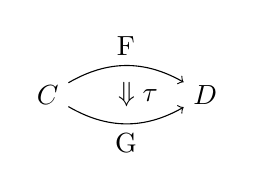
\begin{tikzpicture}
    \node (C) at (-1,0) {$\cat{C}$};
    \node (D) at (1,0) {$\cat{D}$};
    \node (T) at (0,0) {$\;\;\;\Downarrow\tau$};
    \draw[->,bend left] (C) to node [above] {F} (D);
    \draw[->,bend right] (C) to node [below] {G} (D);
  \end{tikzpicture}
\]
such that:
\begin{enumerate}
  \item $\forall X \in \cat{C},
    \exists \tau_X : F(X) \rightarrow G(X) \in \cat{D}$
  \item $\forall f : X \rightarrow Y \in \cat{C},
    \tau_Y \circ F(f) = G(f) \circ \tau_X$
\end{enumerate}
where the Morphism $\tau_X$ is called the \emph{Component} of $\tau$
at $X$. When (2) holds, a Commutative Diagram is formed and the
Morphisms $\tau_X$ are said to be \emph{Natural} in $X$. If there is
no Morphism in $\cat{D}$ corresponding to $\tau_X$, then there can
be no Natural Transformation from $F$ to $G$.

Milewski: A Natural Transformation maps Morphisms to Commuting
Diagrams

When every Component in $\tau$ is Invertible in $\cat{D}$, $\tau$ is a
\emph{Natural Isomorphism} (\S\ref{sec:natural_isomorphism}) and $F
\cong G$. Equivalently, a Natural Isomorphism is an Isomorphism in the
Functor Category $Fun(\cat{C},\cat{D})$.

Natural Isomorphisms:
\[
  Hom_\cat{Grp}(F_1,G) \cong U(G)
\]\[
  Hom_\cat{Set}(X,\cat{2}) \cong \pow(X)
\]\[
  Hom_\cat{BA}(B,\cat{2}) \cong Ult(X)
\]

in Programming Languages, Natural Transformations may be represented
as Polymorphic Functions (i.e. Family of Functions Parameterized by
Types)

Horizontal Composition (\S\ref{sec:horizontal_composition}):
Composition along $1$-morphisms (Functors)

Vertical Composition (\S\ref{sec:horizontal_composition}):
Composition along Objects (Categories)



% --------------------------------------------------------------------
\subsection{Vertical Composition}\label{sec:vertical_composition}
% --------------------------------------------------------------------

Given Natural Transformations $\eta : F \Rightarrow G$ and $\epsilon :
G \Rightarrow H$ between Functors $F,G,H : \cat{C} \rightarrow
\cat{D}$, the \emph{Vertical Composition} is $\epsilon\circ\eta : F
\Rightarrow H$:
\[
  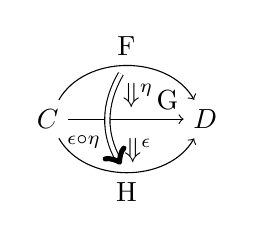
\begin{tikzpicture}
    \node (C) at (-1,0) {$\cat{C}$};
    \node (D) at (1,0) {$\cat{D}$};
    \node (N) at (0,0.3) {$\;\;\;\Downarrow^\eta$};
    \node (M) at (0,-0.4) {$\;\;\;\Downarrow^\epsilon$};
    \node (F) at (0,0.7) {};
    \node (H) at (0,-0.7) {};
    \draw[->,bend left=60] (C) to node [above] {F} (D);
    \draw[->] (C) to node [above] {\quad\quad\quad G} (D);
    \draw[->,bend right=60] (C) to node [below] {H} (D);
    \draw[->,bend right=30,double distance=1.5pt] (F) to
      node [left,pos=0.75] {$_{\epsilon\circ\eta}$} (H);
  \end{tikzpicture}
\]

Composition in the corresponding Functor Category



% --------------------------------------------------------------------
\subsection{Horizontal Composition}\label{sec:horizontal_composition}
% --------------------------------------------------------------------

Given Functors $F,G : \cat{C} \rightarrow \cat{D}$ and $J,K : \cat{D}
\rightarrow \cat{E}$, and Natural Transformations $\eta : F
\rightarrow G$ and $\epsilon : J \rightarrow K$, the \emph{Horizontal
  Composition} (or \emph{Godement Product}) is $\eta * \epsilon : JF
\Rightarrow KG$:
\[
  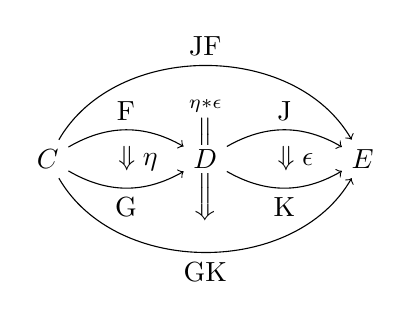
\begin{tikzpicture}
    \node (U) at (0,0) {$\stackrel{\eta*\epsilon}
      {\stackrel{\Big\|}{\Big\Downarrow}}$};
    \node [fill,color=white,scale=1.5] (W) at (0,0) {};
    \node (C) at (-2,0) {$\cat{C}$};
    \node (D) at (0,0) {$\cat{D}$};
    \node (E) at (2,0) {$\cat{E}$};
    \node (S) at (-1,0) {$\;\;\;\Downarrow\eta$};
    \node (T) at (1,0) {$\;\;\;\Downarrow\epsilon$};
    \draw[->,bend left] (C) to node [above] {F} (D);
    \draw[->,bend right] (C) to node [below] {G} (D);
    \draw[->,bend left] (D) to node [above] {J} (E);
    \draw[->,bend right] (D) to node [below] {K} (E);
    \draw[->,bend left=60] (C) to node [above] {JF} (E);
    \draw[->,bend right=60] (C) to node [below] {GK} (E);
  \end{tikzpicture}
\]

Horizontal Composition is Associative and has the same Identity as
Vertical Composition.



% --------------------------------------------------------------------
\subsection{Interchange Law}\label{sec:interchange_law}
% --------------------------------------------------------------------

Given three Categories, $\cat{B}$, $\cat{C}$, and $\cat{D}$,
and six Functors, $P,Q,R : \cat{B} \rightarrow \cat{C}$ and
$S,T,U : \cat{C} \rightarrow \cat{D}$, and four Natural
Transformations, $\sigma : P \rightarrow Q$, $\tau : Q \rightarrow R$,
$\sigma' : S \rightarrow T$, and $\tau' : T \rightarrow U$, the
following \emph{Interchange Law} applies:
\[
  (\tau' \cdot \sigma') \circ (\tau \cdot \sigma) =
  (\tau' \circ \tau) \cdot (\sigma' \circ \sigma)
\]



% --------------------------------------------------------------------
\subsection{Natural Isomorphism}\label{sec:natural_isomorphism}
% --------------------------------------------------------------------

\emph{Natural Equivalence} in a $1$-category %FIXME xref

\[
  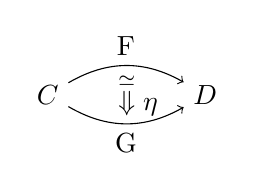
\begin{tikzpicture}
    \node (C) at (-1,0) {$\cat{C}$};
    \node (D) at (1,0) {$\cat{D}$};
    \node (N) at (0,0) {$\;\;\;\stackrel{\simeq}{\Downarrow}\eta$};
    \draw[->,bend left] (C) to node [above] {F} (D);
    \draw[->,bend right] (C) to node [below] {G} (D);
  \end{tikzpicture}
\]

\begin{itemize}
  \item Natural Isomorphism with a Two-sided Inverse (???)
  \item each Component $\eta_X : F(X) \rightarrow G(X)$ for all $X
    \in \cat{C}_0$ is an Isomorphism in $\cat{D}$
  \item Isomorphism in the Functor Category
    (\S\ref{sec:functor_category}) $[\cat{C},\cat{D}]$
\end{itemize}



% --------------------------------------------------------------------
\subsection{Extranatural Transformation}
\label{sec:extranatural_transformation}
% --------------------------------------------------------------------

For Functors $F : \cat{A} \times \cat{B}^{op} \times \cat{B}
\rightarrow \cat{D}$ and $G : \cat{A} \times \cat{C}^{op} \times
\cat{C} \rightarrow \cat{D}$, the Family $\eta(a,b,c) : F(a,b,b)
\rightarrow G(a,c,c)$ is Natural in $a$ and \emph{Extranatural} in $b$
and $c$ if the following holds:
\begin{itemize}
  \item (Natural in $a$): $\eta (-,b,c)$ is a Natural Transformation
  \item (Extranatural in $b$): $\forall (g:b \rightarrow b') \in
    \cat{B}_1, \forall a \in \cat{A}, \forall c \in \cat{C},
    \eta(a,b,c) \circ F(1,1,g) = \eta(a,b',c) \circ F(1,g,1)$
  \item (Extranatural in $c$): $\forall (h:c \rightarrow c') \in
    \cat{C}_1, \forall a \in \cat{A}, \forall b \in \cat{B}, G(1,h,1)
    \circ \eta(a,b,c) = G(1,1,h) \circ \eta(a,b,c')$
\end{itemize}



% --------------------------------------------------------------------
\subsection{Dinatural Transformation}
\label{sec:dinatural_transformation}
% --------------------------------------------------------------------

Ex.: Hughes Arrow (\S\ref{sec:hughes_arrow}) $\ggg : A (X,P) \times A
(P,Y) \rightarrow A (X,Y)$ is Dinatural in $P$. For each $f : P
\rightarrow Q$:
\[
  id \times A(f,id) \circ \ggg = A(id,f) \times id \circ \ggg
\]



% ====================================================================
\section{Opposite Category}\label{sec:opposite_category}
% ====================================================================

The \emph{Opposite} or \emph{Dual} (\S\ref{sec:abstract_category})
of a Category $\cat{C}$ is denoted $\cat{C^{op}}$ or
$\cat{C^*}$ and has the same Objects as $\cat{C}$ but the Domain
and Codomain in each Morphism is reversed. Objects and Morphisms of a
Dual Category may be written with over-lines to distinguish them from
the original Category: $\overline{f}: \overline{C} \rightarrow
\overline{D}$. With this notation the following Equalities may be
expressed:
\[
  1_{\overline{C}} = \overline{1_C}
\]\[
  \overline{f} \circ \overline{g} = \overline{g \circ f}
\]
A Terminal Object in $\cat{C}$ is an Initial Object in
$\cat{C^{op}}$ and vice-versa.

The Functor $(-)^\cat{op} : \cat{Cat} \rightarrow \cat{Cat}$
is an Involution (\S\ref{sec:involution}) but is Contravariant so it
does not define any Isomorphisms.

In a Dual Category the following are all Duals of eachother:
\begin{itemize}
  \item Monomorphisms and Epimorphisms (\S\ref{sec:morphism})
  \item Left and Right Inverses (\S\ref{sec:morphism})
  \item Initial and Terminal Objects (\S\ref{sec:universal_property})
\end{itemize}



% ====================================================================
\section{Category Product}\label{sec:category_product}
% ====================================================================

A \emph{Product}, $\times$, is a Construction (i.e. a Functor,
specifically a Bifunctor \S\ref{sec:bifunctor}) on Categories (or
Functors):
\[
  \times : \cat{Cat} \times \cat{Cat} \rightarrow \cat{Cat}
\]

Product (\S\ref{sec:product})



% --------------------------------------------------------------------
\subsection{Product Category}\label{sec:product_category}
% --------------------------------------------------------------------

A \emph{Product Category} can be constructed from two Categories,
$\cat{C}$ and $\cat{D}$, and is denoted:
\[
  \cat{C} \times \cat{D}
\]
has Objects of the form $(C,D)$ where $C \in \cat{C}$ and $D \in
\cat{D}$ and Morphisms $(f,g) : (C,D) \rightarrow (C',D')$ where $f
: C \rightarrow C' \in \cat{C}$ and $g : D \rightarrow D' \in
\cat{D}$. Composition and Identity are defined as:
\[
  (f',g') \circ (f,g) = (f' \circ f,g' \circ g)
\]\[
  1_{(C,D)} = (1_C, 1_D)
\]
$\cat{C} \times \cat{D}$ is a Product (\S\ref{sec:product}) in
$\cat{Cat}$.



\subsubsection{Projection}\label{sec:projection_functor}

A Product Category has a pair of \emph{Projections} which are Functors
from the Product Category to the original Categories:
\[
  \cat{C} \xleftarrow{\;\; P\;\;} \cat{C}\times\cat{D}
  \xrightarrow{\;\; Q\;\;} \cat{D}
\]
such that for $C,f \in \cat{C}, D,g \in \cat{D}$:
\[
  P(C,D) = C, \;\; P(f,g) = f
\]\[
  Q(C,D) = D, \;\; Q(f,g) = g
\]
Given any other Category, $\cat{B}$, there exists a unique Functor:
\[
  F : \cat{B} \rightarrow \cat{C} \times \cat{D}
\]
with:
\[
  PF = R : \cat{B} \rightarrow \cat{C}
\]\[
  QF = T : \cat{B} \rightarrow \cat{D}
\]
giving:
\[
  \forall h \in B, F(h) = (Rh,Th)
\]



% --------------------------------------------------------------------
\subsection{Functor Product}\label{sec:functor_product}
% --------------------------------------------------------------------

Give two Functors, $U : \cat{C} \rightarrow \cat{C'}$ and $V :
\cat{D} \rightarrow \cat{D'}$, a \emph{Functor Product} is
defined as:
\[
  U \times V : \cat{C} \times \cat{D}
  \rightarrow \cat{C'} \times \cat{D'}
\]
where:
\[
  (U \times V)(C,D) = (UC,VD), \;\; (U \times V)(f,g) = (Uf,Vg)
\]
and $(U \times V)$ is the unique Functor such that:
\[
  P'(U \times V) = UP, \;\; Q'(U \times V) = VQ
\]
%FIXME is the above correct?



% ====================================================================
\section{Quotient Category}\label{sec:quotient_category}
% ====================================================================

%FIXME this probably needs a rewrite

The \emph{Quotient Category} is defined for a Category $\cat{C}$
with Congruence Relation $\sim$ as $\cat{C}/\sim$:
\[
  (\cat{C}/\sim)_0 = \cat{C_0}
\]\[
  (\cat{C}/\sim)_1 = (\cat{C_1})/\sim
\]
where Morphisms are of the form $[f]$ where $f \in \cat{C_1}$.

For a Category $\cat{C}$ with Graph $G$ and relations $R$,
$\cat{C}/R$ is called the Category with \emph{Generators} $G$ and
\emph{Relations} $R$.

Homotopy Category (\S\ref{sec:homotopy_category})



% --------------------------------------------------------------------
\subsection{Congruence Category}\label{sec:congruence_category}
% --------------------------------------------------------------------

\emph{Congruence} on a Category is an Equivalence Relation on
Morphisms such that for two Morphisms $f,g \in \cat{C_1}$, $f \sim
g$ Implies:
\begin{itemize}
  \item $dom(f) = dom(g)$
  \item $cod(f) = cod(g)$
  \item $\forall a,b \in \cat{C_1}, bfa \sim bga$
\end{itemize}
Such a Congruence defines a \emph{Congruence Category}
$\cat{C^{\sim}}$:
\[
  (\cat{C^{\sim}})_0 = \cat{C}_0
\]\[
  (\cat{C^{\sim}})_1 = \{\langle f,g \rangle | f \sim g\}
\]\[
  \tilde{1_\cat{C}} = \langle 1_\cat{C}, 1_\cat{C} \rangle
\]\[
  \langle f',g' \rangle \circ \langle f,g \rangle = \langle f'f,g'g \rangle
\]
The Categorical Congruence $\sim$ on a Group $G$ is a Normal Subgroup
$N \subseteq G$ and the Quotient Category $G/\sim$ and the Quotient
Group $G/N$ coincide. \cite{awodey06}



% --------------------------------------------------------------------
\subsection{Kernel Category}\label{sec:kernel_category}
% --------------------------------------------------------------------

Given a Functor $F : \cat{C} \rightarrow \cat{D}$, a Congruence
$\sim_F$ on $\cat{C}$ is defined as:
\[
  f \sim_F g \leftrightarrow dom(f) = dom(g) \wedge cod(f) = cod(g)
  \wedge F(f) = F(g)
\]
The \emph{Kernel Category} of $F$ is then defined as the Congruence
Category of $\sim_F$
\[
  ker(F) = C^{\sim_F}
\]



% --------------------------------------------------------------------
\subsection{Finitely Presented Category}
\label{sec:finitely_presented}
% --------------------------------------------------------------------

% FIXME free category notation?
A \emph{Finitely Presented Category} is given by taking the Quotient
Category of a Free Category (\S\ref{sec:free_category})
$\cat{C}(G)$ with the Congruence $\sim_\Sigma$:
\[
  \cat{C}(G) / \sim_{\Sigma} = \cat{C}(G,\Sigma)
\]
where $\Sigma$ is the finite Set of Relations:
\[
  (g_1 \circ \ldots \circ g_n) = (g'_1 \circ \ldots \circ g'_m)
\]
for all $g_i \in G$ such that $dom(g_n) = dom(g'_m)$ and $cod(g_1) =
cod(g'_1)$.



% ====================================================================
\section{Arrow Category}\label{sec:arrow_category}
% ====================================================================

An \emph{Arrow Category} of a Category $\cat{C}$, written
$\cat{C^{\rightarrow}}$, has for its Objects the Morphisms of
$\cat{C}$ and as Morphisms pairs of Objects such that their
underlying Morphisms in $\cat{C}$ are Composable (Commutative
Squares).

The Arrow Category $\cat{C}^\rightarrow$ is Isomorphic to the
Functor Category $\cat{C^2}$.

There are two Functors defined on an Arrow Category:
\[
  \cat{C} \xleftarrow{\cat{dom}} \cat{C}^\rightarrow
  \xrightarrow{\cat{cod}} \cat{D}
\]

Equivalent to the Comma Category (\S\ref{sec:comma_category})
$(1_\cat{C}/1_\cat{C})$



% ====================================================================
\section{Comma Category}\label{sec:comma_category}
% ====================================================================

A \emph{Comma Category} is formed from a pair of Functors that share a
common Codomain. For three Categories, $\cat{A}$, $\cat{B}$, and
$\cat{C}$ and Functors $S$ (\emph{Source}) and $T$ (\emph{Target}) in
the following relation:
\[
  \cat{A} \xrightarrow{\;\; S\;\;} \cat{C} \xleftarrow{\;\;
    T\;\;} \cat{B}
\]
one can form a Comma Category $(S \downarrow T)$ with Objects as
Triples $(\alpha, \beta, f)$ where $\alpha$ is an Object in
$\cat{A}$, $\beta$ is an Object in $\cat{B}$, and $f : S(\alpha)
\rightarrow T(\beta)$ is a Morphism in $\cat{C}$ and with Morphisms
between Triples $(\alpha, \beta, f)$ to $(\alpha', \beta', f')$ as
pairs $(g,h)$ where $g : \alpha \rightarrow \alpha'$ is a Morphism in
$\cat{A}$ and $h : \beta \rightarrow \beta'$ is a Morphism in
$\cat{B}$.

When $S$ is a Functor, $\cat{1} \xrightarrow{\;\;S\;\;}
\cat{C}$, to a single Object $A \in \cat{C}$, the resulting
Comma Category may be denoted $(A \downarrow \cat{C})$ and is
called the Category of Objects under $A$. Here Objects are Morphisms
with Domain of $A$, and Morphisms are Commutative triangles with top
Vertex $A$.

The Category of Objects over $A$ is likewise $(\cat{C} \downarrow
A)$ and has as Objects Morphisms with Codomain $A$ and Morphisms are
Commutative triangles with a bottom Vertex $A$.

When both $S$ and $T$ are Functors from $\cat{1}$ to Objects $A$
and $B$ respectively, the result is a Discrete Category whose Objects
are $Hom(A,B)$.

The case where $S = T = 1_\cat{C}$, $(\cat{C} \downarrow
\cat{C})$, is the Category of all Morphisms of $\cat{C}$:
$\cat{C}^\cat{2}$.



% --------------------------------------------------------------------
\subsection{Slice Category}\label{sec:slice_category}
% --------------------------------------------------------------------

A \emph{Slice Category} (or \emph{Overcategory}) $\cat{C}/C$ of a
Category $\cat{C}$ with an Object $C$ has as Objects the Morphisms
with Codomain $C$ and as Morphisms those Morphisms in $\cat{C}$
between the Domains of the underlying Morphisms of the Objects of
$\cat{C}/C$. That is, for Objects in the Slice Category corresonding
to Morphisms $f$ and $f'$, the Morphism in the Slice Category between
the two is $g$ such that
\[
  f' \circ g = f
\]

\emph{Coslice}

if each Slice Category $\cat{C}/x$ is a Cartesian Monoidal Category
(\S\ref{sec:cartesian_monoidal}) then $\cat{C}$ is Locally Cartesian
(\S\ref{sec:locally_cartesian})

Categorical Semantics (\S\ref{sec:categorical_semantics}) for Formal
Logic (Part \ref{part:formal_logic}) and Type Theory (Part
\ref{part:type_theory})



% --------------------------------------------------------------------
\subsection{Coslice Category}\label{sec:coslice_category}
% --------------------------------------------------------------------



% ====================================================================
\section{Bifunctor}\label{sec:bifunctor}
% ====================================================================

A \emph{Bifunctor} is a Functor of two Variables from a Product
Category to an arbitrary Category:
\[
  B : \cat{C} \times \cat{D} \rightarrow \cat{A}
\]

A \emph{Multifunctor} is a generalized to $n$ or more Variables.



% --------------------------------------------------------------------
\subsection{Product Functor}\label{sec:product_functor}
% --------------------------------------------------------------------

\[
  \times : \cat{C} \times \cat{C} \rightarrow \cat{C}
\]

Category Product (\S\ref{sec:category_product})



% --------------------------------------------------------------------
\subsection{Coproduct Functor}\label{sec:coproduct_functor}
% --------------------------------------------------------------------

\[
  + : \cat{C} \times \cat{C} \rightarrow \cat{C}
\]



% --------------------------------------------------------------------
\subsection{Diagonal Functor}\label{sec:diagonal_functor}
% --------------------------------------------------------------------

For Functor Category (\S\ref{sec:functor_category})
$\cat{C}^\cat{J}$ with Small Index Category $\cat{J}$, a
\emph{Diagonal Functor} $\Delta : \cat{C} \rightarrow
\cat{C}^\cat{J}$ assigns to each Object $A$ of $\cat{C}$ the
Constant Functor $\Delta_A \in \cat{C}^\cat{J}$ with fixed $A$
and to each Morphism $f : A \rightarrow B$ of $\cat{C}$ the Natural
Transformation $\eta$ in $\cat{C}^\cat{J}$ given by $\eta_j =
f$.

If $\cat{J}$ is a Discrete Category with two Objects, the Diagonal
Functor is $\cat{C} \rightarrow \cat{C} \times \cat{C}$.

The Limit (\S\ref{sec:limit}) of a Functor $F : \cat{J} \rightarrow
\cat{C}$ is a Universal Morphism (\S\ref{sec:universal_morphism})
from the Diagonal Functor $\Delta$ to $F$.

If $\cat{C}$ is Complete (\S\ref{sec:complete_category}) then every
Functor from $\cat{J}$ to $\cat{C}$ has a Limit and the
operation of taking Limits is a Functor from $\cat{C}^\cat{J}$
to $\cat{C}$.

The Limit Functor is the Right-adjoint (\S\ref{sec:adjoint_functor})
of the Diagonal Functor.

A Colimit (\S\ref{sec:colimit}) is a Universal Morphism $F \rightarrow
\Delta$.

If $\cat{C}$ is Complete the Colimit Functor exists and is the
Left-adjoint of the Diagonal Functor.

As an example, the Diagonal Functor $\cat{C} \rightarrow \cat{C}
\times \cat{C}$ is the Left-adjoint of the Binary Product Functor
(\S\ref{sec:product_functor}) and the Right-adjoint of the Binary
Coproduct Functor (\S\ref{sec:coproduct_functor}).



% --------------------------------------------------------------------
\subsection{Profunctor}\label{sec:profunctor}
% --------------------------------------------------------------------

A \emph{Profunctor} (or \emph{Distributor}) is a Bifunctor that is
Contravariant in the first argument and Covariant in the second.

Generalization of Functors, Categorical generalization of Bimodules
(\S\ref{sec:bimodule})

$P : \cat{C} \nrightarrow \cat{D}$

$H_P : \cat{D}^{op} \times \cat{C} \rightarrow \cat{Set}$

Set of Heteromorphisms (\S\ref{sec:heteromorphism})

Identity Profunctor $Id : \cat{C} \nrightarrow \cat{C}$ is given by
the Hom-functor $\cat{C}(-,-) : \cat{C}^{op} \times \cat{C}
\rightarrow \cat{Set}$

Composition of Profunctors $P : \cat{C} \nrightarrow \cat{D}$, $Q :
\cat{D} \nrightarrow \cat{E}$:
\[
  Q P = \int^{d \in \cat{D}} P(d,-) \otimes Q(-,d)
\]
% FIXME kan extensions?

Every Functor $F : \cat{C} \rightarrow \cat{D}$ induces two
Profunctors $D(1,F) : \cat{C} \nrightarrow \cat{D}$ and $D(F,1)
: \cat{D} \nrightarrow \cat{C}$ where $D(1,F)(d,c) = D(d,f(c))$
and $D(f,1)(c,d) = D(f(c),d)$.

Functor $F : \cat{C} \rightarrow \cat{D}$ gives a Profunctor $P_F :
\cat{C} \nrightarrow \cat{D}$ by Post-composition with the Yoneda
Functor (\S\ref{sec:yoneda_embedding}):
\[
  P_F = Y_\cat{D} \circ F
\]



\subsubsection{Profunctor Bicategory}\label{sec:profunctor_bicategory}

Bicategory (\S\ref{sec:bicategory}) of Profunctors

Coend (\S\ref{sec:coend})



% ====================================================================
\section{Hom-functor}\label{sec:hom_functor}
% ====================================================================

A \emph{Hom-functor} is a Functor from a Locally Small Category
(\S\ref{sec:locally_small}), $\cat{C}$, to the Category $\cat{Set}$,
and has a Covariant and a Contravariant definition:

\begin{enumerate}
  \item \emph{Covariant Hom-functor}, for $A \in \cat{C}_0$, $f : X
    \rightarrow Y \in \cat{C}_1$:
\[
\begin{split}
  & h^A = Hom(A,-) : \cat{C} \rightarrow \cat{Set} \\
  & X \mapsto Hom(A,X) \\
  & f \mapsto Hom(A,f) : Hom(A,X) \rightarrow Hom(A,Y)
\end{split}
\]
  where $Hom(A,f)$ is defined for all $g \in Hom(A,X)$ as:
\[
  g \mapsto f \circ g
\]

  \item \emph{Contravariant Hom-functor} (also \emph{Functor of
    Points}, see Generalized Elements
    \S\ref{sec:generalized_element}), for $B \in \cat{C}_0$, $f : X
    \rightarrow Y \in \cat{C}_1$:
\[
\begin{split}
  & h_B = Hom(-,B) : \cat{C} \rightarrow \cat{Set} \\
  & X \mapsto Hom(X,B) \\
  & f \mapsto Hom(f,B) : Hom(Y,B) \rightarrow Hom(X,B)
\end{split}
\]
  where $Hom(f,B)$ is defined for all $g \in Hom(Y,B)$ as:
\[
  g \mapsto g \circ f
\]
\end{enumerate}

The Hom-functor $Hom(-,-)$ is a Covariant Bifunctor
(\S\ref{sec:bifunctor}):
\[
  Hom_\cat{C}(-,-):
    \cat{C}^{op} \times \cat{C} \rightarrow \cat{Set}
\]
each half of which is a Representable Functor
(\S\ref{sec:representable_functor}). $Hom_\cat{C}(-,-)$ is also the
Identity Profunctor (\S\ref{sec:profunctor}) $1_\cat{C} :
\cat{C} \nrightarrow \cat{C}$. Hom-functors are Continuous
Functors (\S\ref{sec:continuous_functor}).

The Category of all Hom-functors and Natural Transformations
(\S\ref{sec:natural_transformation}) between them, $\{ h^A | A \in
\cat{C} \}$, is a Subcategory of the Functor Category
(\S\ref{sec:functor_category}) $\cat{Set^C}$, and is Isomorphic to
$\cat{C^{op}}$ (see Yoneda Embedding \S\ref{sec:yoneda_embedding}).

Every Morphism $f : A' \rightarrow A$ determines a pair of Natural
Transformations:
\[
  Hom(f,-) : h^A \rightarrow h^{A'}
\]\[
  Hom(-,f) : h_{A'} \rightarrow h_A
\]

For any pair of Morphisms, $f : A' \rightarrow A$ and $g : B
\rightarrow B'$:
\[
  Hom(A',g) \circ Hom(f,B) = Hom(f,B') \circ Hom(A,g)
\]
is a path sending:
\[
  h : A \rightarrow B
\]
to:
\[
  g \circ h \circ f : A' \rightarrow B'
\]



% --------------------------------------------------------------------
\subsection{Closed Category}\label{sec:closed_category}
% --------------------------------------------------------------------

A \emph{Closed Category} is a Category $\cat{C}$ with:
\begin{itemize}
  \item Internal Hom-functor (\S\ref{sec:internal_hom}):
    \[
      [-,-]:\cat{C}^{op} \times \cat{C} \rightarrow \cat{C}
    \]
  \item Unit Object:
    \[
      I \in \cat{C}_0
    \]
  \item Natural Isomorphism:
    \[
      i : 1_\cat{C} \cong [I,-]
    \]
  \item Transformation:
    \[
      j_X : I \rightarrow [X,X]
    \]
    Extranatural (\S\ref{sec:extranatural_transformation}) in $X$
  \item Transformation:
    \[
      L_{Y Z}^X : [Y,Z] \rightarrow [[X,Y],[X,Z]]
    \]
    Natural in $Y$ and $Z$ and Extranatural in $X$
\end{itemize}
Satisfying the Axioms:
\begin{enumerate}
  \item $L_{Y Y}^X \circ j_Y = j_{[X,Y]}$ for any $X,Y$
  \item $[j_X,1] \circ L_{X Y}^X = i_{[X,Y]}$ for any $X,Y$
  \item $[i_Y,1] \circ L_{Y Z}^I = [1,i_Z]$ for any $Y,Z$
  \item $[1,L_{Y V}^X] \circ L_{U V}^Y = [L_{Y U}^X,1] \circ L_{[X,U]
    [X,V]}^{[X,Y]} \circ L_{U V}^X$ for any $X,Y,U,V$
  \item The Map $\gamma : \cat{C}(X,Y) \rightarrow \cat{C}(I,[X,Y])$
    defined by $f \mapsto [1,f](j_X)$ is a Bijection
\end{enumerate}

Every Closed Category embeds Fully and Faithfully into a Closed
Monoidal Category (\S\ref{sec:closed_monoidal}) by a Strong Closed
Functor (LaPlaza) %FIXME



\subsubsection{Internal Hom-functor}\label{sec:internal_hom}

\emph{Internal Hom Functor}
\[
  [-,-] : \cat{C}^{op} \times \cat{C} \rightarrow \cat{C}
\]



\subsubsection{Dualizing Object}\label{sec:dualizing_object}

\emph{Dualizing Object} $D$ in a Closed Category $\cat{D}$ is an
Object with Internal Hom $[-,D]: \cat{C} \rightarrow \cat{C}^{op}$ an
Involutive Duality Operation on $\cat{C}$: %FIXME
\[
  [[-,D],D]: \cat{C} \rightarrow \cat{C}
\]

Dual Object (\S\ref{sec:dual_object})



% --------------------------------------------------------------------
\subsection{Representable Functor}\label{sec:representable_functor}
% --------------------------------------------------------------------

%FIXME definition of 'representation'
%FIXME ref Naturally Isomorphic
Presheaf (\S\ref{sec:category_presheaf})

A Functor $F : \cat{C} \rightarrow \cat{Set}$ is a
\emph{Representable Functor} if it is Naturally Isomorphic to the
Hom-functor $h^A$ or $h_A$ for some Object $A \in \cat{C}$.

A \emph{Covariant Representable Functor} for an Object $A$ in a
Category $\cat{C}$ is defined as Naturally Isomorphic to the
Covariant Hom-functor $h^A = Hom(A,-) : \cat{C} \rightarrow
\cat{Set}$
\[
  Hom(A,-) : Hom(A,X) \xrightarrow{f_*} Hom(A,Y)
\]
A \emph{Contravariant Representable Functor} for $A$ is a Functor that
is Naturally Isomorphic to the Contravariant Hom-functor $h_A =
Hom(-,A) : \cat{C^{op}} \rightarrow \cat{Set}$
\[
  Hom(-,A) : Hom(X,A) \xrightarrow{f^*} Hom(Y,A)
\]

A \emph{Representation} of a Covariant Representable Functor, $F$, is
a pair $(A, \Phi)$ with Natural Isomorphism $\Phi : Hom(A,-)
\rightarrow F$.

Contravariant Representable Functors map all Colimits
(\S\ref{sec:colimit}) to Limits (\S\ref{sec:limit}).

A Locally Small Category (\S\ref{sec:locally_small}) has Representable
Functors for all Objects.

generalization of Upper Sets (\S\ref{sec:upper_set}) in Posets



% --------------------------------------------------------------------
\subsection{Locally Small Category}\label{sec:locally_small}
% --------------------------------------------------------------------

A Category is \emph{Locally Small} if all Hom-sets
(\S\ref{sec:hom_set}) of the Category are Sets and not Proper Classes.
% FIXME definition in terms of hom-sets

Hom-functor (\S\ref{sec:hom_functor})

There is at least one canonical Representable Functor
(\S\ref{sec:representable_functor}) from any Locally Small Category
into $\cat{Set}$.

For a Locally Small Category $\cat{C}$, $\cat{Set^{C^{op}}}$ is
Complete (\S\ref{sec:complete_category}) and Cocomplete
(\S\ref{sec:cocomplete_category}) and for all $C \in \cat{C}_0$,
the Evaluation Functor $ev_C : \cat{Set^{C^{op}}} \rightarrow
\cat{Set}$ preserves all Limits. \cite{awodey06}



% ====================================================================
\section{Concrete Category}\label{sec:concrete_category}
% ====================================================================

A \emph{Concrete Category} is pair, $(\cat{C},U)$, where $\cat{C}$ is
a Category and $U$ is a Faithful Functor
(\S\ref{sec:faithful_functor}) $U : \cat{C} \rightarrow \cat{Set}$.

Representable Functor (\S\ref{sec:representable_functor})

Sets with Structure (\S\ref{sec:abstract_structure})

Categories with Interpretations as Concrete Categories:
\begin{itemize}
  \item $\cat{Set}$
  \item $\cat{Top}$
  \item $\cat{Grp}$
\end{itemize}

Not \emph{Concretizable}:
\begin{itemize}
  \item $\cat{Toph}$
\end{itemize}



% ====================================================================
\section{Yoneda Lemma}\label{sec:yoneda_lemma}
% ====================================================================

For an arbitrary Covariant Functor $F : \cat{C} \rightarrow
\cat{Set}$:
\[
  Nat_\cat{Set^C}(h^A,F) \cong F(A)
\]
If $F$ is a Covariant Hom-functor $h^B$, then:
\[
  Nat_\cat{Set^C}(h^A,h^B) \cong Hom(B,A)
\]

For an arbitrary Contravariant Functor $G : \cat{C}^{op} \rightarrow
\cat{Set}$:
\[
  Nat_\cat{Set^{C^op}}(h_B,G) \cong G(A)
\]
If $F$ is a Contravariant Hom-functor $h_B$, then:
\[
  Nat_\cat{Set^{C^{op}}}(h_A,h_B) \cong Hom(A,B)
\]

Corollary:
\[
  yA \cong yB \Rightarrow A \cong B
\]



% --------------------------------------------------------------------
\subsection{Yoneda Embedding}\label{sec:yoneda_embedding}
% --------------------------------------------------------------------

The Fully Faithful Contravariant Functor $h^- : \cat{C} \rightarrow
\cat{Set^C}$ which maps each Object $A \in \cat{C}_0$ to the
Hom-functor $h^A$ and each $f \in \cat{C}_1$ to the Natural
Transformation $Hom(f,-)$ can also be interpreted as a Covariant
Functor $h^- : \cat{C^{op}} \rightarrow \cat{Set^C}$. Being a
Faithful Functor means $h^-$ gives an Embedding
(\S\ref{sec:category_embedding}) of $\cat{C^{op}}$ in
$\cat{Set^C}$.

By the Contravariant Yoneda's Lemma:
\[
  h_-: \cat{C} \rightarrow \cat{Set^{C^{op}}}
\]
called the \emph{Yoneda Embedding}.

Covariant:

$Nat_\cat{Set^C}(Hom(A,-), Hom(B,-)) \cong Hom_\cat{C}(B,A)$

Contravariant:

$Nat_\cat{Set^{C^op}}(Hom(-,A), Hom(-,B)) \cong Hom_\cat{C}(A,B)$

Yoneda Embedding preserves all Products and Exponentials in
$\cat{C}$.



% --------------------------------------------------------------------
\subsection{Coyoneda}\label{sec:coyoneda}
% --------------------------------------------------------------------

Free Functor (\S\ref{sec:free_functor})



% ====================================================================
\section{Functor Category}\label{sec:functor_category}
% ====================================================================

Given two Categories, $\cat{C}$ and $\cat{D}$, a \emph{Functor
  Category} is a Category with Objects as Functors $T : \cat{C}
\rightarrow \cat{D}$ and Morphisms as Natural Transformations
between Functors:
\[
  \cat{D}^{\cat{C}} = Fun(\cat{C},\cat{D})
\]

$[\cat{C},\cat{D}]$

A Hom-set in a Functor Category may be denoted:
\[
  Nat(S,T) = \cat{D}^{\cat{C}}(S,T) =
    \{ \tau | \tau : S \rightarrow T \}
\]

With Evaluation Functor $\eta : \cat{D^C} \times \cat{C} \rightarrow
\cat{D}$, $\cat{D^C}$ is an Exponential
(\S\ref{sec:category_exponential}) in $\cat{Cat}$ and $\cat{Cat}$ is a
Cartesian Closed Category (\S\ref{sec:cartesian_closed}).

The Functor Category $\cat{C^2}$ is Isomorphic to Arrow Categories
(\S\ref{sec:arrow_category}) $\cat{C}^\rightarrow$.

The Functor Category $\cat{C}^\cat{2}$ from the Discrete Category
$\cat{2}$ is equivalent to the Product Category $\cat{C} \times
\cat{C}$.

For any Discrete Category $I$:
\[
  \cat{C}^I \cong \prod_{i \in I} \cat{C}
\]

The Functor Category $\cat{Set}^\downdownarrows$ where
$\downdownarrows$ is the Category with two Objects and two Morphisms
between them ($* \rightrightarrows \star$) is equivalent to the
Category of Graphs and Graph Homomorphisms $\cat{Graph}$. Cf.
Simplicial Sets (\S\ref{sec:simplicial_set}).

A Functor Category into the Category $\cat{Set}$ is called a
\emph{Category Diagram} (\S\ref{sec:category_diagram}).
%FIXME terminology doesn't match



% --------------------------------------------------------------------
\subsection{Set-valued Functor Category}\label{sec:setvalued_functor}
% --------------------------------------------------------------------

A \emph{Set-valued Functor Category} (or \emph{Category of Diagrams})
is a Functor Category from a Category into the Category
$\cat{Set}$.

A Presheaf (\S\ref{sec:presheaf}) is an example of a Set-valued
(Contravariant) Functor Category from an Opposite Category into
$\cat{Set}$.



\subsubsection{Powerset Functor}\label{sec:powerset_functor}

$\pow : \cat{Set} \rightarrow \cat{Set}$

Functions $f : X \rightarrow Y$ to the Image Mapping $img(f) :
\pow(X) \rightarrow \pow(Y)$



% ====================================================================
\section{Presheaf Category}\label{sec:presheaf_category}
% ====================================================================

Objects: Functors $F: \cat{C}^{op} \rightarrow \cat{Set}$

Morphisms: Natural Transformations $\Phi : F \rightarrow G$

$Psh(\cat{C}) = [\cat{C}^{op},\cat{Set}]$



% --------------------------------------------------------------------
\subsection{Presheaf}\label{sec:category_presheaf}
% --------------------------------------------------------------------

A \emph{Presheaf} is a Contravariant Functor from an Opposite Category
to the Category $\cat{Set}$. A Presheaf is an example of a
Set-valued Functor Category (\S\ref{sec:category_diagram}) and gives a
Cartesian Closed Category (\S\ref{sec:cartesian_closed}).

Presheaf (Topology \S\ref{sec:presheaf})

$2$-presheaf (\S\ref{sec:2_presheaf})

Sheave (\S\ref{sec:sheave})



% --------------------------------------------------------------------
\subsection{Copresheaf}\label{sec:copresheaf}
% --------------------------------------------------------------------



% --------------------------------------------------------------------
\subsection{Representable Presheaf}\label{sec:representable_presheaf}
% --------------------------------------------------------------------

Limit (\S\ref{sec:limit})



% --------------------------------------------------------------------
\subsection{Graphic Category}\label{sec:graphic_category}
% --------------------------------------------------------------------

Class of Finite Monoids and Categories permitting a ``graphic
display'' via Presheaf (\S\ref{sec:presheaf}) Categories
(def. nCat Lab) % FIXME

Graphic Monoid (\S\ref{sec:graphic_monoid})



% ====================================================================
\section{Universal Property}\label{sec:universal_property}
% ====================================================================

Unique up to Unique Isomorphism



% --------------------------------------------------------------------
\subsection{Universal Mapping Property}
\label{sec:universal_mapping_property}
% --------------------------------------------------------------------

A \emph{Universal Mapping Property} is a Property in the Language of
Category Theory that defines a Mathematical Structure up to
Isomorphism. By relation to the Curry-Howard Correspondence, these
Isomorphisms are effectively two-way Rules of Inference.

\emph{Existence}

\emph{Uniqueness}

Universal Construction

Milewski: If a Universal Construction exists for all Diagrams of a
certain shape in a Category, it can also be defined through an
Adjunction (\S\ref{sec:adjunction})



% --------------------------------------------------------------------
\subsection{Universal Morphism}\label{sec:universal_morphism}
% --------------------------------------------------------------------

Given a Functor $S: \cat{D} \rightarrow \cat{C}$, an
\emph{Universal Morphism} to $S$ or \emph{Initial Morphism}, is an
Initial Object of the form $(Y',u)$ in the Comma Category
(\S\ref{sec:comma_category}) $(X \downarrow S)$ where $X \in
\cat{C}_0$, $u : X \rightarrow S(Y') \in \cat{C}_1$ and $X' \in
\cat{D}_0$.
%FIXME is X' initial and/or terminal in D?

$(Y', u)$ satisfies the \emph{Initial Property}:
\[
  \forall Z' \in \cat{D}, \forall f : X \rightarrow S(Z') \in
  \cat{C}, \exists! g : Y' \rightarrow Z' : S(g) \circ u = f
\]

The Dual concept of an Initial Morphism, an Universal Morphism from
$S$ or \emph{Terminal Morphism}, is a Terminal Object of the form
$(X',v)$ in the Comma Category $(S \downarrow X)$ where $v : S(X')
\rightarrow X \in \cat{C}$.

$(X',v)$ satisfies the \emph{Terminal Property}:
\[
  \forall Y' \in \cat{D}, \forall f : S(Y') \rightarrow X \in
  \cat{C}, \exists! g : Y' \rightarrow X' : v \circ S(g) = f
\]

%FIXME universality in terms of Hom sets



\subsubsection{Universal Element}\label{sec:universal_element}

\emph{Representable Functor} (\S\ref{sec:representable_functor})

For a Functor $H : \cat{D} \rightarrow \cat{Set}$, an
\emph{Universal Element} of $H$ is a pair of Objects $(A,X) \in
\cat{D}_0 \times \cat{Set}_0$ such that:
\[
  \forall (A',X') \in \cat{D}_0 \times \cat{Set}_0,
  \exists! f : A \rightarrow A' \in \cat{D} : H(f)(X) = X'
\]



% --------------------------------------------------------------------
\subsection{Global Element}\label{sec:global_element}
% --------------------------------------------------------------------

A \emph{Global Element}, $a$, (also \emph{Point} or \emph{Constant})
of an Object, $A$, is a Morphism from a Terminal Object, $1$, to that
Object
\[
  a: 1 \rightarrow A
\]
In $\cat{Set}$ this expresses an Isomorphism:
\[
  A \cong Hom_\cat{Set}(1,A)
\]
but is not true for all Categories in general.

In some settings Global Elements represent Closed Terms.

Pointed Object (\S\ref{sec:pointed_object})



\subsubsection{Well-pointed Category}\label{sec:well_pointed}

Well-pointed Topos (\S\ref{sec:wellpointed_topos})



% --------------------------------------------------------------------
\subsection{Generalized Element}\label{sec:generalized_element}
% --------------------------------------------------------------------

A \emph{Generalized Element} (or \emph{General Element} or
\emph{Variable}) $x$ is a Morphism from an arbitrary Domain Object,
$X$:
\[
  x: X \rightarrow A
\]

In some contexts Generalized Elements correspond to arbitrary Terms
(\S\ref{sec:term}) as in Programming Languages (``Computational
Trinitarianism'', Curry-Howard Correspondence
\S\ref{sec:curry_howard}).



% --------------------------------------------------------------------
\subsection{Separator}\label{sec:separator}
% --------------------------------------------------------------------

(or \emph{Generator})

nLab:

Object $S$ (or Family of Objects $\class{S}$) in a Category $\cat{C}$
for which Generalized Elements (\S\ref{sec:generalized_element}) with
Domain $S$ (or $\class{S}$) are ``sufficient'' to distinguish
Morphisms in $\cat{C}$.

Grothendieck Categories (\S\ref{sec:grothendieck_category})



\subsubsection{Coseparator}\label{sec:coseparator}



% --------------------------------------------------------------------
\subsection{Category Diagram}\label{sec:category_diagram}
% --------------------------------------------------------------------

A \emph{Category Diagram} is a Covariant Functor from an \emph{Index
  Category} into another Category:
\[
  D : \cat{J} \rightarrow \cat{C}
\]
A Diagram is the Category Theory analogue of an Indexed Family of Sets
(\S\ref{sec:index_set}).

Category of Diagrams (\S\ref{sec:setvalued_functor})

$Diag(\cat{C},\cat{D})$



\subsubsection{Cone}\label{sec:category_cone}

A \emph{Cone} in a Diagram $D : \cat{J} \rightarrow \cat{C}$ is
an Object $C \in \cat{C}_0$ and a Unique Morphism $c_j : C
\rightarrow D_j$ for each Object in the Diagram such that any
resulting triangles Commute.

This is equivalent to a Natural Tranformation from the Constant
Functor (\S\ref{sec:constant_functor}) $\Delta_C$ to the Diagram
Functor $D$.

Cone Category $\cat{Cone}(D)$

Cocone (\S\ref{sec:cocone})



\paragraph{Universal Cone}\label{sec:universal_cone}\hfill

Universal Object in the Cone Category

Cone Category $\cat{Cone}(D)$

A Limit (\S\ref{sec:limit}) is a Terminal Object in the Cone
Category.



\subsubsection{Cocone}\label{sec:cocone}

A \emph{Cocone} in a Diagram $D : \cat{J} \rightarrow \cat{C}$
is an Object $C \in \cat{C}_0$ and a Unique Morphism $c_j : D_j
\rightarrow C$ for each Object in the Diagram such that any resulting
triangle Commutes.




\paragraph{Universal Cocone}\label{sec:universal_cocone}\hfill

Universal Object in the Cocone Category

Cocone Category $\cat{Cocone}(D)$

A Colimit (\S\ref{sec:colimit}) is a Initial Object in the Cocone
Category.



\subsubsection{Wedge}\label{sec:wedge}

$T : \cat{C}^{op} \times \cat{C} \rightarrow \cat{D}$

\emph{Wedge}, $X \in \cat{D}$ with Family of Morphisms $\omega_C :
X \rightarrow T(C,C)$ in $\cat{D}$ for all $C \in \cat{C}$ such
that for any $f : C \rightarrow C'$ in $\cat{C}$:
\[
  \omega_C \circ T(1_C,f) = \omega_C' \circ T(f,1_{C'})
\]
(Extranatural Transformation \S\ref{sec:extranatural_transformation}

$\omega_C(X) = n_C : C \rightarrow C$ are Components of a Natural
Transformation from $1_\cat{C} \rightarrow 1_\cat{C}$. A Wedge
$X \xrightarrow{.} Hom : \cat{C}^{op} \times \cat{C} \rightarrow
\cat{Set}$ is a Function $X \rightarrow Nat
(1_\cat{C},1_\cat{C})$.

A Universal Wedge is called an \emph{End} (\S\ref{sec:end})



\subsubsection{Span}\label{sec:span}

\emph{Span} (or \emph{Roof} or \emph{Correspondence})

Span from Object $X$ to Object $Y$ in a Category $\cat{C}$, with
another Object $S$:
\[
  X \xleftarrow{\quad f \quad} S \xrightarrow{\quad g \quad} Y
\]

generalization of Relations: a Correspondence which is
$(-1)$-truncated (\S\ref{sec:truncation}) as a Morphism into the
Cartesian Product

Diagram over $1 \rightarrow 2 \leftarrow 3$

The Colimit of a Span is a Pushout (\S\ref{sec:pushout})

Spans can be Composed in a Category with Pullbacks
(\S\ref{sec:pullback})



\paragraph{Correspondence Category}\label{sec:correspondence_category}\hfill

Category of Spans

$\cat{Corr_C}$

Self-dual: if Limits Exist, Colimits also Exist and vice versa



\subsubsection{Cospan}\label{sec:cospan}

The Limit of a Cospan is a Pullback (\S\ref{sec:pullback})



\subsubsection{Category of Elements}\label{sec:element_category}

For all $P \in \cat{Set^{C^{op}}}$, $P$ is a Colimit of
Representable Functors:
\[
  \lim_{\rightarrow_j} yA_j \cong P
\]
by the Yoneda Lemma (\S\ref{sec:yoneda_lemma})

Index Category: $\int_\cat{C} P$

Objects: $(x,C)$ where $C \in \cat{C}_0$ and $x \in PC$

Morphisms: Triples $(h, (x',C'), (x,C))$ where $h : C' \rightarrow C
\in \cat{C}_1$ such that $P(h)(x) = x'$.

Projection Functor: $\pi : \int_\cat{C} P \rightarrow \cat{C}$
such that $\pi(x,C) = C$ and $\pi(h, (x',C'), (x,C)) = h$



% --------------------------------------------------------------------
\subsection{Limit}\label{sec:limit}
% --------------------------------------------------------------------

\emph{Limit} = \emph{Inverse Limit} = \emph{Projective Limit} =
\emph{Left Root}

\emph{Colimit} = \emph{Direct Limit} = \emph{Inductive Limit} =
\emph{Right Root}

Colimit (\S\ref{sec:colimit})

A \emph{Limit} is defined as a Terminal Object in the Cone Category
(\S\ref{sec:category_cone}) over a Diagram $D : \cat{J} \rightarrow
\cat{C}$:
\[
  c_i : \lim_{\xleftarrow[j]{}} D_j \rightarrow D_i
\]

A Category has all Finite Limits if and only if it has Finite Products
(\S\ref{sec:category_product}) and Equalizers (\S\ref{sec:equalizer}),
or equivalently if it has Pullbacks (\S\ref{sec:pullback}) and a
Terminal Object (\S\ref{sec:terminal_object}). Furthermore, a Category
has all Limits of som Cardinality if and only if it has all Equalizers
and Products of that Cardinality. \cite{awodey06}

A Limit is also definable as a Natural Isomorphism (a Natural
Transformation with every Component an Isomorphism) between the two
Functors:
\[
  \cat{C}(c, \lim_{\xleftarrow[j]{}} D) \cong Nat (\Delta_c, D)
\]

Representable Presheaf (\S\ref{sec:representable_presheaf})



\subsubsection{Finite Limit}\label{sec:finite_limit}

Limit over a Finite Diagram, i.e. one whose shape is a Finite Category
(\S\ref{sec:finite_category})



\subsubsection{Terminal Object}\label{sec:terminal_object}

An Object $1$ in a Category $\cat{C}$ is \emph{Terminal} if for
every other Object $A$ in the Category there is a unique Morphism $A
\rightarrow 1$. A Unique, Canonical Isomorphism exists between any two
Terminal Objects in $\cat{C}$.

As an example, in $\cat{Set}$ and $\cat{Pos}$, all Singleton
Sets are Terminal, and as such they are all Isomorphic to each other.
Given a Set $X$:
\[
  |X| = 1 \leftrightarrow \forall Y, |Hom_{\cat{Set}}(Y,X)| = 1
\]

In a Poset, a Top Element is a Terminal Object.



\subsubsection{Product}\label{sec:product}

A \emph{Product} of two Objects $P = A \times B$:
\[
  A \xleftarrow{\;\;p_1\;\;} P \xrightarrow{\;\;p_2\;\;} B
\]
is a Product of $A$ and $B$ if and only if for any $A
\xleftarrow{\;\;z_1\;\;} Z \xrightarrow{\;\;z_2\;\;} B$:
\[
  \exists!u : Z \rightarrow P
\]
with $p_i \circ u = z_i$. $u$ is called a \emph{Factorization} and may
also be written as $\langle z_1, z_2 \rangle$ as it is uniquely
determined by $z_1$ and $z_2$.

A Product of two Categories is uniquiely Isomorphic to the Cartesian
Product (\S\ref{sec:cartesian_product}) of the two Sets.

In a Poset, the Product of two Elements is the Meet or Greatest Lower
Bound (\S\ref{sec:greatest_lowerbound}).

For Morphisms $f$ and $g$, a Product $f \times g$ is defined where $f
: A \rightarrow A'$, $g : B \rightarrow B'$ and:
\[
  f \times g : A \times B \rightarrow A' \times B' =
  \langle f \circ p_1, g \circ p_2 \rangle
\]
with $p_1$ and $p_2$ the Projections $p_1 : A \times B \rightarrow A$
and $p_2 : A \times B \rightarrow B$.

A Category $\cat{C}$ with Binary Products between any two Objects
has a \emph{Product Functor} (\S\ref{sec:product_functor}):
\[
  \times : \cat{C} \times \cat{C} \rightarrow \cat{C}
\]
which Maps pairs of Objects of $\cat{C}$ to their Product:
\[
  (A,B) \mapsto A \times B
\]
and Morphisms of $\cat{C}$ to their Product:
\[
  (f,g) \mapsto f \times g
\]
A Category with Binary Products and a Terminal Object is said to have
all \emph{Finite Products}. It is possible to Model the Theory of
Groups (\S\ref{sec:group_theory}) in any Category with all Finite
Products.

A Category has Finite Products and Equalizers if and only if it has
Pullbacks (\S\ref{sec:pullback}) and a Terminal Object. \cite{awodey06}

Products are unique up to Isomorphism (\S\ref{sec:isomorphism}). The
Canonical Commutative Isomorphism $A \times B \cong B \times A$ is:
\[
  \langle p_2, p_1 \rangle : A \times B \rightarrow B \times A
\]
which is the Natural Transformation $\theta$ betwen the Product
Functor and the \emph{Twisted Product Functor} $\tilde{\times} :
\cat{C} \times \cat{C} \rightarrow \cat{C}$ (Mapping $(A,B)
\mapsto B \times A$):
\[
  \theta : \times \rightarrow \tilde{\times}
\]

The Universal Mapping Property for Products may be stated as a two-way
Rule of Inference:
\[
  {
    \frac{X \rightarrow A \;\;\;\; X \rightarrow B}
    {X \rightarrow A \times B}
  }\times
\]

Products are also Associative:
\[
  A \times (B \times C) \cong (A \times B) \times C
\]

In $\cat{Set}$ the Product is the Cartesian Product $\times$ and the
Unit is the Singleton Set $1$.

In $\cat{Rel}$ the Product is the Direct Sum $+$ and the Unit is
the Empty Set $\varnothing$.

In $\cat{Hilb}$ the Product is Binary Sum and the Unit is the
Zero-dimensional Hilbert Space $\{ 0 \}$. %FIXME products not
                                %isomorphic? strict monoidal category



\paragraph{N-ary Products}\label{sec:category_nary}\hfill
A Terminal Object is a \emph{Nullary Product}. A general Object is its
own \emph{Unary Product}.

By Associativity of Products, $A \times B \times C = (A \times B)
\times C$ so any Category that has Binary Products also has all
\emph{Finite N-ary Products}.



\paragraph{Diagonal}\label{sec:diagonal}\hfill

\emph{Diagonal} of an Object $X$ in a Category with Products is the
canonical Morphism:
\[
  \Delta : X \xrightarrow{(\Id,\Id)} X \times X
\]

\fist Cf. Codiagonal (\S\ref{sec:codiagonal})



\subsubsection{Equalizer}\label{sec:equalizer}

An \emph{Equalizer} is an (Unique) Object $E$ and Morphism $e: E
\rightarrow A$ such that for a given pair of Parallel Morphisms $f,g :
A \rightarrow B$:
\[
  f \circ e = g \circ e
\]
$e$ is necessarily a Monomorphism.

Limit of Parallel Morphisms

For a Set $X$ in $\cat{Set}$, every Subset $U \subseteq X$ occurs
as an Equalizer.

The Category $\cat{Ab}$ has all Equalizers.

If a Category has Binary Products (\S\ref{sec:category_product}) and
Equalizers then it has Pullbacks (\S\ref{sec:pullback}).



\paragraph{Kernel}\label{sec:morphism_kernel}\hfill

The \emph{Kernel} of a Morphism $f : X \rightarrow Y$ is the most
general Morphism $k : K \rightarrow X$ such that $fk = 0_{KY}$ and for
any Morphism $k' : K' \rightarrow X$ such that $fk' = 0_{K'Y}$, there
exists a unique Morphism $u : K' \rightarrow K$ such that $ku = k'$.

A Kernel is a special case of an Equalizer where one of the Morphisms
is a Zero Morphism (\S\ref{sec:zero_morphism}).



\paragraph{End}\label{sec:end}\hfill

\emph{End} of a Functor is a Universal Wedge (\S\ref{sec:wedge}) $E
\xrightarrow{.} T$ where $T : \cat{C}^{op} \times \cat{C}
\rightarrow \cat{D}$ and $E \in \cat{D}$

$\int_{C \in \cat{C}} T(C,C)$

The End of $Hom : \cat{C}^{op} \times \cat{C} \rightarrow
\cat{Set}$ is $Nat (1_\cat{C},1_\cat{C})$ called the
\emph{Hochschild Cohomology} \S\ref{sec:hochschild_homology} or
\emph{Symmetries} of $\cat{C}$.

For two Functors $F,G : \cat{C} \rightarrow \cat{E}$, the End for
the Functor $\cat{E}(F(-), G(-)) : \cat{C}^{op} \times
\cat{C} \rightarrow \cat{Set}$ is:
\[
  \int_{C \in \cat{C}} \cat{E}(F(C), G(C)) = Nat (F,G)
\]

Forgetful Functor, Tannakian Reconstruction
(\S\ref{sec:tannakian_category}) %FIXME tannakian reconstruction
Monoid $(M,\mu,\eta)$, $\int_{(M,\mu,\eta)} \cong M$



\subsubsection{Pullback}\label{sec:pullback}

For a Category $\cat{C}$, a \emph{Pullback} (or \emph{Fiber
  Product} or \emph{Cartesian Square}) of Morphisms $f : A \rightarrow
C$ and $g : B \rightarrow C$ are Morphisms $p_1 : P \rightarrow A$ and
$p_2 : P \rightarrow B$ with the Universal Property that $fp_1 =
g_p2$. This implies for any given $z_1 : Z \rightarrow A$ and $z_2 : Z
\rightarrow B$ such that $fz_1 = gz_2$, there is a Unique Morphism $u
: Z \rightarrow P$ such that $z_1 = p_1 u$ and $z_2 = p_2 u$.

Categorical Semantics of an Equation (\S\ref{sec:equation})

In $\cat{Set}$ a Pullback is a Subset of the Cartesian Product of two
Sets: for the Diagram with $A,B,C$ Sets and Functions $f : A
\rightarrow C$, $g : B \rightarrow C$, a Pullback is the Subset $X
\subseteq A \times B$ of Pairs $(a,b)$ such that $f(a) = g(b)$.

A Pullback is the Limit of a Cospan (\S\ref{sec:cospan}).

Subtyping (\S\ref{sec:subtype})

Type Inference (\S\ref{sec:type_inference}) (Unification)

generalization of Intersection (\S\ref{sec:set_intersection}) and
Inverse Image (\S\ref{sec:preimage})

Dependent Sum (\S\ref{sec:dependent_sum}) over the Dependent Equality
Type (\S\ref{sec:dependent_equality}):
\[
  \sum_{a:A} \sum_{b:B} (f(a) = g(b))
\]

A Category has Pullbacks and a Terminal Object if and only if it has
Finite Products (\S\ref{sec:category_product}) and Equalizers
(\S\ref{sec:equalizer}). \cite{awodey06}

Base Change Functor (\S\ref{sec:base_change})



\paragraph{Reindexed Family}\label{sec:reindexed_family}\hfill

Indexed Family (\S\ref{sec:indexed_family})



\paragraph{Display Map}\label{sec:display_map}\hfill

Display Map Category (\S\ref{sec:display_map_category}): Categorical
Semantics (\S\ref{sec:categorical_semantics}) of Dependent Types
(\S\ref{sec:dependent_type})

$b : B \rightarrow A$

$B \type$ Dependent on Variable of Type $A$:

$x:A \vdash B(x):\mathrm{Type}$



\subparagraph{Display Class}\label{sec:display_class}\hfill

For Category $\cat{C}$ a Class of Morphisms of $\cat{C}$, $\class{D}
\subset \cat{C}_1$, is a \emph{Class of Displays} if all Pullbacks
(\S\ref{sec:pullback}) of Elements of $\class{D}$ exist and belong to
$\class{D}$.



\subsubsection{Cotensor Product}\label{sec:cotensor_product}

Monoidal Category (\S\ref{sec:monoidal_category})



\paragraph{Power}\label{sec:power}\hfill

Covariant Powerset Functor % FIXME

Cumulative Hierarchy (\S\ref{sec:cumulative_hierarchy})

$Hom(X,\cat{2}) \cong \pow(X)$

Ultrafilters (\S\ref{sec:ultrafilter})

$Ult(B) \cong Hom_\cat{BA}(B,\cat{2})$

Adjoint Functors:

$Ult : \cat{BA}^{op} \rightarrow \cat{Set}$

$\pow^\cat{BA} : \cat{Set}^{op} \rightarrow \cat{BA}$

Natural Transformations (\S\ref{sec:natural_transformation}) from
Stone Duality (\S\ref{sec:stone_duality}):
\[
  \eta_X : X \rightarrow Ult(\pow(X))
\]\[
  \phi_B : B \rightarrow \pow(Ult(B))
\]

$\pow^\cat{BA} :
  \cat{Set}^{op}_{fin} \rightarrow \cat{BA}_{fin}$

$A : \cat{BA}^{op}_{fin} \rightarrow \cat{Set}_{fin}$
\emph{Atoms} of a Boolean Algebra:
\[
  A(\mathcal{B}) = \{ a \in \mathcal{B} \;|\;
    0 < a, (b < a \Rightarrow b = 0) \}
\]
There is an Isomorphism between Atoms $a$ of a Finite Boolean Algebra
$\mathcal{B}$ and Ultrafilters $U \subseteq \mathcal{B}$:
\[
  U \mapsto \bigwedge_{b \in U} b
\]\[
  a \mapsto \uparrow (a)
\]



\subsubsection{Inverse Limit}\label{sec:inverse_limit}



% --------------------------------------------------------------------
\subsection{Colimit} \label{sec:colimit}
% --------------------------------------------------------------------

Adjoint Functor (\S\ref{sec:adjoint_functor})

Diagonal Functor (\S\ref{sec:diagonal_functor})

Small Limit

A \emph{Colimit} is defined as a Universal Cone
(\S\ref{sec:universal_cone})

A Category has Finite Colimits if and only if it has Finite Coproducts
(\S\ref{sec:coproduct}) and Coequalizers (\S\ref{sec:coequalizer}).
Likewise, a Category has all Colimits of some Cardinality $\kappa$ if
and only if it has Coequalizers and Coproducts of Cardinality
$\kappa$.



\subsubsection{Initial Object}\label{sec:initial_object}

An Object $0$ in a Category $\cat{C}$ is \emph{Initial} if for
every other Object $A$ in the Category there is a unique Morphism $0
\rightarrow A$. A Unique Canonical Isomorphism exists between any two
Initial Objects in $\cat{C}$.

An Initial Object is the Colimit of the Empty Diagram $\varnothing
\rightarrow \cat{C}$

In $\cat{Set}$ the Empty Set is Initial as the only mapping from it
to any other Set is the Empty Function.

In a Poset, the Bottom Element is an Initial Object.

All Universal Properties are Initial Objects somewhere...
%FIXME catsters



\subsubsection{Coproduct}\label{sec:coproduct}

$X,Y \in \cat{C}_0$, $X \amalg Y \in \cat{C}_0$

The Diagram $A \xrightarrow{\;\;q_1\;\;} Q \xleftarrow{\;\;q_2\;\;} B$
is a \emph{Coproduct} $A + B$ if for any $A \xrightarrow{\;\;z_1\;\;}
Z \xleftarrow{\;\;z_2\;\;} B$:
\[
  \exists!u : Q \rightarrow Z
\]
with $u \circ q_i = z_i$. $u$ may also be written as $[ z_1, z_2 ]$
and Coprojections $q_i$ may be called \emph{Injections} (although they
are not necessarily Injective Morphisms).

The Universal Mapping Property for Coproducts may be stated as a
two-way Rule of Inference:
\[
  {
    \frac{A \rightarrow X \;\;\;\; B \rightarrow X}
    {A + B \rightarrow X}
  }+
\]

An example of a Coproduct in $\cat{Set}$ is the Disjoint Union
(\S\ref{sec:disjoint_union}) in Set Theory or the Tagged Union
(\S\ref{sec:sum_type}) in Type Theory. The Coproduct of a Monoid is
sometimes defined as a Tensor Product (\S\ref{sec:tensor_product}). In
a Poset the Coproduct of two Elements is the Join or Least Upper Bound
(\S\ref{sec:least_upperbound}).

\begin{itemize}
\item $\cat{Set}$: Disjoint Union (\S\ref{sec:disjoint_union})
\item $\cat{Pos}$: Join (Least Upper Bound
  \S\ref{sec:least_upperbound})
\item $\cat{Grp}$: Free Product (\S\ref{sec:free_product})
\item $\cat{Ab}$, $\cat{Vect}$: Direct Sum (\S\ref{sec:direct_sum})
\item $\cat{Top}$: Disjoint Union Topology
  (\S\ref{sec:disjoint_union_topology})
\item Pointed Spaces: Wedge Sum (\S\ref{sec:wedge_sum})
\item Type Theory: Sum Type (\S\ref{sec:sum_type})
\end{itemize}

In the Category $\cat{Ab}$ there is a Canonical
Isomorphism:\cite{awodey06}
\[
  A + B \cong A \times B
\]



\paragraph{Codiagonal}\label{sec:codiagonal}\hfill

\emph{Codiagonal} (or \emph{Fold Morphism}) of an Object $X$ in a
Category with Coproducts:
\[
  \nabla : X \amalg X \xrightarrow{(\Id,\Id)} X
\]

\fist Cf. Diagonal (\S\ref{sec:diagonal})



\subsubsection{Coequalizer}\label{sec:coequalizer}

An \emph{Coequalizer} is an (Unique) Object $Q$ and Morphism $q: B
\rightarrow Q$ such that for a given pair of Parallel Morphisms $f,g :
A \rightarrow B$:
\[
  q \circ f = q \circ g
\]
$q$ is necessarily an Epimorphism.

Colimit of Parallel Morphisms

A Coequalizer in a Category $\cat{C}$ is an Equalizer in
$\cat{C}$ and \emph{vice versa}.

The Categories $\cat{Set}$ and $\cat{Pos}$ have all
Coequalizers.

Quotient (\S\ref{sec:equivalence_class})



\paragraph{Quotient Object}\label{sec:quotient_object}\hfill

\paragraph{Cokernel}\label{sec:cokernel}\hfill

\paragraph{Coend}\label{sec:coend}\hfill

of a Functor $S : \cat{C}^{op} \times \cat{C} \rightarrow
\cat{X}$, a Pair $(d, \zeta)$ with Object $d \in \cat{X}_0$ and
Extranatural Transformation (\S\ref{sec:extranatural_transformation})
$\zeta : S \xrightarrow{..} d$



\subsubsection{Pushout}\label{sec:pushout}

A Pushout is the Colimit of a Span (\S\ref{sec:span})

$B +_A C \cong (B + C)/\sim$

In $\cat{Set}$ a Pushout is a Quotient of the Disjoint Union of two
Sets: in a Diagram with $A,B,C$ Sets and Functions $f : C \rightarrow
A$ and $g : C \rightarrow B$, the Pushout is the Disjoint Union $A +
B$ with $a \in A \sim b \in B$ when there Exists $x \in C$ such that
$f(x) = a$ and $g(x) = b$. When $C$ is the Intersection of $A$ and $B$
(and $f$ and $g$ are the Inclusions), the Pushout is equal to $A + B$.



\subsubsection{Tensor Product}\label{sec:tensor_product}

For a Monoidal Category (\S\ref{sec:monoidal_category}) $\cat{M}$,
a \emph{Tensor Product} is a Functor:
\[
  \otimes : \cat{M} \times \cat{M} \rightarrow \cat{M}
\]

Cartesian Product in $\cat{Set}$

``Freest'' Bilinear Operator (\S\ref{sec:bilinear_map}):
\begin{itemize}
\item Modules: Module Tensor (\S\ref{sec:module_tensor})
\item Vector Spaces (\S\ref{sec:vector_space}): Outer Product
  (\S\ref{sec:outer_product})
\end{itemize}

Vertically Categorified (\S\ref{sec:vertical_categorification}) Monoid



\paragraph{Copower}\label{sec:copower}\hfill

\paragraph{Tensorial Strength}\label{sec:tensorial_strength}\hfill

Natural Transformation $\tau_{A,B} : A \otimes F B \rightarrow F (A
\otimes B)$
%FIXME commutative diagrams

Strong Functor (\S\ref{sec:strong_functor})

Strong Monad (\S\ref{sec:strong_monad})



\subsubsection{Direct Limit}\label{sec:direct_limit}

\paragraph{$\omega$-colimit}\label{sec:omega_colimit}\hfill

$\omega$-colimit $G_\infty$

Forgetful Functor $U : \cat{Grp} \rightarrow \cat{Set}$ creates
$\omega$-colimits (and all Limits). \cite{awodey06}



\subsubsection{Cocomplete Category}\label{sec:cocomplete_category}

A \emph{Cocomplete Category} is a Category where all Small Colimits
exist.

For any Categories $\cat{C}$ and $\cat{D}$, if $\cat{D}$ is
Cocomplete, then the Functor Category $\cat{D^C}$ is Cocomplete and
for every $C \in \cat{C}$, the Evaluation Functor $ev_C :
\cat{D^C} \rightarrow \cat{D}$ preserves Colimits.

For any Locally Small Category (\S\ref{sec:locally_small})
$\cat{C}$ the Functor Category $\cat{Set^{C^{op}}}$ is
Cocomplete.

For a Cocomplete Category $\mathcal{E}$ and Functor $F : \cat{C}
\rightarrow \mathcal{E}$, there is a Unique (up to Natural
Isomorphism) Colimit Preserving Functor $F_! : \cat{Set^{C^{op}}}
\rightarrow \mathcal{E}$ such that $F_! \circ y \cong A$ where $y$ is
the Yoneda Embedding (\S\ref{sec:yoneda_embedding}).\cite{awodey06}
%FIXME what is `A` here?



% --------------------------------------------------------------------
\subsection{Zero Object}\label{sec:zero_object}
% --------------------------------------------------------------------

An Object that is both an Initial and a Terminal Object is called a
\emph{Zero Object} (or \emph{Null Object}). A Category with a Zero
Object is called a \emph{Pointed Category}
(\S\ref{sec:pointed_category}).

For a Zero Object, $Z \in \cat{C}$, there is a Unique Morphism
between any two Objects, $A, B \in \cat{C}$ called the
\emph{Composite} in $Z$:
\[
  A \rightarrow Z \rightarrow B
\]

In $\cat{Grp}$, a Trivial Group ${1}$ is a Zero Object.



\subsection{Pointed Category}\label{sec:pointed_category}



% --------------------------------------------------------------------
\subsection{Exponential}\label{sec:category_exponential}
% --------------------------------------------------------------------

Given a Category $\cat{C}$ with Binary Products between any two
Objects:
\[
  \exists \times_{A,B} \forall A,B \in \cat{C}
\]
an \emph{Exponential Object} (\S\ref{sec:exponential_object}) $B^A$
with a Universal Morphism (\S\ref{sec:universal_morphism}) (sometimes
called ``eval'' or ``apply''):
\[
  \epsilon : B^A \times A \rightarrow B
\]
such that:
\[
  \forall X, f \in \cat{C}, \exists ! \lambda f :
  \epsilon \circ (\lambda f \times 1_A) = f
\]
where $\lambda f \times 1_A : X \times A \rightarrow B^A \times A$ is
called the \emph{Exponential Transpose} of $f$. The Morphisms $f$ and
$\lambda f$ are called \emph{Exponential Adjoints}. The $\epsilon$
function is the Counit of the Adjunction (\S\ref{sec:adjunction}) between
the Product Functor and the Exponential Functor.

The Universal Mapping Property for Exponentials implies the two-way
Rule of Inference:
\[
  {
    \frac{X \times A \rightarrow B}
    {X \rightarrow B^A}
  }exp
\]
From this the following Two-way Inference Rule may be Derived:
\[
    \frac{1 \times A \rightarrow B}
    {1 \rightarrow B^A}
\]

An Exponential $B^A$ corresponds to the Function Space
(\S\ref{sec:function_space}) from $A$ to $B$. For $A,B \in
\cat{Set}_0$ in the Category of Sets, the Exponential $B^A$ is
equal to the Hom-set (\S\ref{sec:hom_set}) $Hom(A,B)$.

In a Poset such as a Propositional Calculus, the Exponential
corresponds to Implication:
\[
    \frac{x \leq b \Rightarrow a}
    {x \wedge a \leq b}
\]

Exponentials do not exists for Group Homomorphisms but they do for
Groupoids (\S\ref{sec:groupoid}).

A Category with an Exponential for any two Objects and a Terminal
Object (\S\ref{sec:terminal_object}) is a Cartesian Closed Category
(\S\ref{sec:cartesian_closed}). In a Cartesian Closed Category the
Functor sending $B$ to $B^A$ is the Right-adjoint Functor
(\S\ref{sec:adjoint_functor}) $- \times Y$ and there is a Bijection
between Hom-sets $Hom(X \times A, B)$ and $Hom(X, B^A)$:
\[
  Hom(X \times A, B) \cong Hom(X, B^A)
\]

An Exponential can also be introduced by a Morphism between Morphisms
called ``curry'' which is equivalent to $\lambda$ above:
\[
  curry : C^{A \times B} \rightarrow (C^B)^A
\]
In a Cartesian Closed Category such as Simply-typed Lambda Calculus
(\S\ref{sec:simply_typed}), all the Morphisms are Internal, so $curry$
corresponds to an Object:
\[
  curry : ((C^B)^A)^{C^{A \times B}}
\]



\subsubsection{Exponential Functor}\label{sec:exponential_functor}

$-^A : \cat{C} \rightarrow \cat{C}$



% --------------------------------------------------------------------
\subsection{Directed Limit}\label{sec:directed_limit}
% --------------------------------------------------------------------

Accessible Category (\S\ref{sec:accessible_category})



% --------------------------------------------------------------------
\subsection{Filtered Limit}\label{sec:filtered_limit}
% --------------------------------------------------------------------

Filtered Colimit

Accessible Functor (\S\ref{sec:accessible_functor})



% --------------------------------------------------------------------
\subsection{Biproduct}\label{sec:biproduct}
% --------------------------------------------------------------------

both Product (\S\ref{sec:product}) and Coproduct
(\S\ref{sec:coproduct})

Category with a Zero Object (\S\ref{sec:zero_object})

any Category with Biproducts is Semi-additive
(\S\ref{sec:semiadditive_category})



% --------------------------------------------------------------------
\subsection{Base Change}\label{sec:base_change}
% --------------------------------------------------------------------

For a Moprhism $f : X \rightarrow Y$ in a Category $\cat{C}$ with
Pullbacks (\S\ref{sec:pullback}), a \emph{Base Change Functor} is an
Induced Functor:
\[
  f^* : \cat{C}/Y \rightarrow \cat{C}/X
\]
of Slice Categories (\S\ref{sec:slice_category}) with:
\[
  f^* = (Z \xrightarrow{\alpha} C) \mapsto
    (X \times_\cat{C} Z \xrightarrow{\alpha^*} X)
\]
%FIXME

If $\cat{C}$ is a Topos then it refines to an Essential Geometric
Morphism (\S\ref{sec:essential_geometric})


Cobase Change

$f_! \dashv f^* \dashv f_*$

$\Sigma_f \dashv f^* \dashv \Pi_f$



\subsubsection{Dependent Product}\label{sec:dependent_product}

Dependent Product Type (\S\ref{sec:pi_type})

Category with all Dependent Products necessarily has all Pullbacks
(\S\ref{sec:pullback})



\subsubsection{Dependent Sum}\label{sec:dependent_sum}

Dependent Sum Type (\S\ref{sec:sigma_type})



% --------------------------------------------------------------------
\subsection{Dependency Morphism}\label{sec:dependency_morphism}
% --------------------------------------------------------------------

\emph{Trace Monoid} (\S\ref{sec:trace_monoid})



% --------------------------------------------------------------------
\subsection{Kan Extension}\label{sec:kan_extension}
% --------------------------------------------------------------------

Wiki: Generalizes the notion of Extending a Function defined on a
Subset to a Function defined on the whole Set.

Categories $\cat{A}, \cat{B}, \cat{C}$

Fuctors $X : \cat{A} \rightarrow \cat{C}, F : \cat{A} \rightarrow
\cat{B}$

Right Kan Extension $Ran$ of $X$ along $F$ is a Functor $R : \cat{B}
\rightarrow \cat{C}$ and a Natural Transformation $\eta : RF
\Rightarrow X$ and Couniversal such that for any Functor $M : \cat{B}
\rightarrow \cat{C}$ and Natural Transformation $\mu : MF \rightarrow
X$ there is a Unique Natural Transformation $\delta : M \rightarrow R$
such that:
\[
  \mu = \eta \circ \delta_F
\]
where $\delta_F$ is the Natural Transformation with $\delta_F(a) =
\delta (F a) : M F(a) \rightarrow RF(a)$ for any Object $a \in
\cat{A}_0$. The Functor $R$ may also be written $\mathrm{Ran}_F X$.

Left Kan Extension $Lan$

Adjoint (\S\ref{sec:adjunction}) as Kan Extension

Limit (\S\ref{sec:limit}) as Kan Extension

Codensity Monad (\S\ref{sec:codensity_monad})

``Constrained Optimization'' % FIXME



% ====================================================================
\section{Adjunction}\label{sec:adjunction}
% ====================================================================

% Adjointness

Two Functors $F : \cat{C} \rightarrow \cat{D}$ and $U : \cat{D}
\rightarrow \cat{C}$ are \emph{Adjoints} when there is a Natural
Isomorphism:
\[
  \Phi : Hom_\cat{D}(F C,D) \cong Hom_\cat{C}(C,U D) : \Psi
\]
is Natural in $C$ and $D$.


Milewski: If a Universal Construction (\S\ref{sec:universal_property})
exists for all Diagrams of a certain shape in a Category, it can also
be defined through an Adjunction


\textbf{Unit}

Natural Transformation:
\[
  \eta : 1_\cat{C} \rightarrow U F
\]

\fist Unit may be called ``Return'' or ``Pure'' in a Monad
(\S\ref{sec:monad})


\textbf{Counit}

Natural Transformation:
\[
  \epsilon : F U \rightarrow 1_\cat{D}
\]

\fist Counit may be called ``Extract'' in a Comonad


Milewski: Unit allows the ``introduction'' of $R \circ L$ anywhere
$\Id_\cat{D}$ would be used; Counit allows an ``elimination'' of the
Composition $L \circ R$ replacing it with $\Id_\cat{C}$. Every Monad
or Comonad may be ``Factorized'' (not necessarily uniquely) into a
pair of Adjoint Functors.


\textbf{Triangle Identities} (\S\ref{sec:triangle_identity})
\[
  \epsilon F \circ F \eta = 1_F
\]\[
  U \epsilon \circ \eta U = 1_U
\]


Universal Mapping Property (\S\ref{sec:universal_property}) for $\eta
: 1_\cat{C} \rightarrow U \circ F$ (Unit):
\begin{itemize}
\item For any $C \in \cat{C}$, $D \in \cat{D}$, $f : C
  \rightarrow U D$, there exists a unique $g : FC \rightarrow D$ such
  that:
  \[
    f = U g \circ \eta_C
  \]
\end{itemize}

Universal Mapping Property for $\epsilon : F \circ U \rightarrow
1_\cat{D}$ (Counit):
\begin{itemize}
\item For any $C \in \cat{C}$, $D \in \cat{D}$, $g : F C
  \rightarrow D$, there exists a unique $f : C \rightarrow U D$ such
  that:
  \[
    g = \epsilon_D \circ F f
  \]
\end{itemize}

Relation between Hom-set and Unit definitions:
\[
  \Phi(g) = U g \circ \eta_C
\]\[
  \eta_C = \Phi(1_{FC})
\]

Relation between (Inverse) Hom-set and Unit definitions:
\[
  \Psi (f) = \epsilon_D \circ F f
\]\[
  \epsilon_D = \Psi(1_{U D})
\]

When Unit and Counit are Natural Isomorphisms
(\S\ref{sec:natural_isomorphism}), the Adjunction is an \emph{Adjoint
  Equivalence} (\S\ref{sec:adjoint_equivalence}).

Free Functors (\S\ref{sec:free_functor}) are Left Adjoint to Forgetful
Functors (\S\ref{sec:forgetful_functor}): Free Functor $\dashv$
Forgetful Functor

In a Cartesian Closed Category (\S\ref{sec:cartesian_closed}), the
following Functors are Adjoints:
\[
  + \dashv \Delta \dashv \times
\]
and:
\[
  (-) \times A \dashv (-)^A
\]
In First-order Logic (Provability $\vdash$):
\[
  \exists \dashv \star \dashv \forall
\]

Adjoint Logic (\S\ref{sec:adjoint_logic})



% --------------------------------------------------------------------
\subsection{Adjoint Functor}\label{sec:adjoint_functor}
% --------------------------------------------------------------------

An \emph{Adjoint Functor} is the Categorical analog of the Existential
Quantifier in Logic (\S\ref{sec:quantifier}) and the Image Operation
along a Continuous Function in Topology (Part \ref{sec:topology}).

Left Adjoint Functors Preserve Colimits (\S\ref{sec:colimit}) and
Epimorphisms (\S\ref{sec:epimorphism})

Right Adjoint Functors Preserve Limits (\S\ref{sec:limit}) and
Monomorphisms (\S\ref{sec:monomorphism})

nLab:

Left and Right Adjoint Functors are ``best approximations'' of Weak
Inverses (\S\ref{sec:weak_inverse})

Left Adjoint: may be thought of as being defined ``Freely''; consists
of anything an Inverse might ``need'' regardless of whether it
``works''.

Right Adjoint: may be thought of as being defined ``Cofreely'';
consists of anything that ``works'' in an Inverse regardless of
whether it's ``needed''.

A Forgetful Functor (\S\ref{sec:forgetful_functor}) has as
Left-adjoint a Free Functor (\S\ref{sec:free_functor}) and as
Right-adjoint a Cofree Functor (\S\ref{sec:cofree_functor})

A Forgetful Functor $G$, forgetting some Constraint $C$, has a
Left-adjoint $F$ that is a ``Free $C$ Functor'' %FIXME



\subsubsection{Triangle Identity}\label{sec:triangle_identity}

\emph{Triangle Identity} (or \emph{Zigzag Identity})
\[
  \epsilon F \circ F \eta = 1_F
\]\[
  U \epsilon \circ \eta U = 1_U
\]



% --------------------------------------------------------------------
\subsection{Adjoint Equivalence}\label{sec:adjoint_equivalence}
% --------------------------------------------------------------------

``Coherent'', ``Structured'' Equivalence

Adjunction $F \dashv G$ where Unit and Counit are Natural Isomorphisms
(\S\ref{sec:natural_isomorphism})

Weak Inverse (\S\ref{sec:weak_inverse})



% --------------------------------------------------------------------
\subsection{Adjoint Triple}\label{sec:adjoint_triple}
% --------------------------------------------------------------------

\subsubsection{Adjoint Cylinder}\label{sec:adjoint_cylinder}

Adjoint Triple such that the outer two Adjoints are Full
(\S\ref{sec:full_functor}) and Faithful (\S\ref{sec:faithful_functor})
Functors

Equivalently: the Induced Adjoint Pair on the Codomain of these
Inclusions (???) consists of an Idempotent Monad and Comonad (Adjoint
Monads \S\ref{sec:adjoint_monad})

Adjoint Modalities (\S\ref{sec:adjoint_modality})



% --------------------------------------------------------------------
\subsection{Reflection}\label{sec:reflection_adjunction}
% --------------------------------------------------------------------

\cite{winskel-nielsen93}

Right-adjoint is Full and Faithful



% --------------------------------------------------------------------
\subsection{Coreflection}\label{sec:coreflection_adjunction}
% --------------------------------------------------------------------

\cite{winskel-nielsen93}

Left-adjoint is Full and Faithful



% ====================================================================
\section{Monad}\label{sec:monad}
% ====================================================================

A \emph{Monad} is given by the Triple:
\[
  (T, \eta, \mu)
\]
where $T : \cat{C} \rightarrow \cat{C}$ is an Endofunctor and $\eta :
1_\cat{C} \rightarrow T$ and $\mu : T^2 \rightarrow T$ (where $T^2 = T
\circ T : \cat{C} \rightarrow \cat{C}$) are Natural Transformations,
called \emph{Unit} and \emph{Multiplication} resp., satisfying the
Coherence Conditions (\S\ref{sec:coherence_condition}):
\begin{enumerate}
  \item $\mu \circ T\mu = \mu \circ \mu T : T^3 \rightarrow T$
  \item $\mu \circ T\eta = \mu \circ \eta T = 1_T : T \rightarrow T$
\end{enumerate}
(1) is analogous to Associativity in Monoids and (2) gives the
existence of an Identity Element.

For every Object $X \in \cat{C}_0$, the Component of the Unit at $X$
is a Morphism:
\[
  \eta_X : X \rightarrow T (X)
\]

Horizontal Categorification (\S\ref{sec:horizontal_categorification})
of a Monoid

A Monad on $\cat{C}$ can be defined as a Monoid Object
(\S\ref{sec:monoid_object}) on the Endofunctor Category
(\S\ref{sec:endofunctor_category}) $\cat{End_C}$.

special case of a Hughes Arrow (\S\ref{sec:hughes_arrow}) with
``output'' but no ``input''

Pointed Endofunctor (\S\ref{sec:pointed_endofunctor}) $S : \cat{C}
\rightarrow \cat{C}$ with Natural Transformation $\sigma : 1_\cat{C}
\rightarrow S$ as the Unit; Well-pointed exactly when the Monad is
Idempotent (\S\ref{sec:idempotent_monad})

A Monad $T$ also arises as a Composition $G \circ F$ of Adjoint
Functors $F : \cat{C} \rightarrow \cat{D}$ and $G : \cat{D}
\rightarrow \cat{C}$, namely $T = G \circ F$ and the Unit of the Monad
is equivalent to the Unit of the Adjunction. If $F$ and $G$ are
Inverses then the corresponding Monad is the Identity Functor.

Given a Monad $T$ on a Category $\cat{C}$, there is a Category of
Adjunctions (\S\ref{sec:adjunction}) that give rise to that Monad.

A $T$-algebra (\S\ref{sec:t_algebra}) for a Monad $T$ is a Model
(\S\ref{sec:model}) of the Algebraic Theory
(\S\ref{sec:algebraic_theory}) given by a Monad.

Correspondences: \cite{jacobs-heunen-hasuo09}
\begin{itemize}
\item Monoids in $\cat{Cat}(\cat{C},\cat{C})$
\item Monads $M$ on $\cat{C}$
\item Identity-on-objects Functors $J : \cat{C} \rightarrow \cat{D}$
  having Right Adjoints (see Kleisli Categories
  \S\ref{sec:kleisli_category})
\end{itemize}

In Programming: Interface to Abstract Datatype
(\S\ref{sec:abstract_type}) of ``Program Fragments''

$\mathsf{return} : X \rightarrow T(X)$ (Comonad: $\textsf{extract}$)

$\mathsf{join} : T(T(X) \rightarrow T(X)$ (Comonad:
$\textsf{duplicate} : T(X) \rightarrow T(T(X))$)

$\mathsf{bind} : T(X) \rightarrow (X \rightarrow T(Y)) \rightarrow
T(Y)$ (Comonad: $\mathsf{cobind} : T(X) \rightarrow (T(X) \rightarrow
Y) \rightarrow T(Y)$)

An alternative to Monads for Computational Effects
(\S\ref{sec:computational_effect}) is Algebraic Effects
(\S\ref{sec:algebraic_effect}), more often seen in Strict Languages
(Algebraic Effects as a Subclass of Computational Effects
\cite{plotkin-pretnar09})

Layered Monads (\S\ref{sec:layered_monad}) \cite{filinski99}

\fist See also Graded Monads (\S\ref{sec:graded_monad}), Parametric
Effect Monads (\S\ref{sec:parametric_effect_monad}), Joinads
(\S\ref{sec:joinad})

Pointed Endofunctor (\S\ref{sec:pointed_endofunctor}) where $\sigma$
is the Unit

Operads (\S\ref{sec:operad}) ``Operations Monads''


\asterism


Comonad (\S\ref{sec:comonad})

Monadic Adjunction (\S\ref{sec:monadic_adjunction})

Terminal Object %FIXME terminal object required in category?

Generalization of Closure Operators on Posets (\S\ref{sec:poset}) to
arbitrary Categories (Galois Connections \S\ref{sec:galois_connection}
as Adjoint Pairs)

Continuation (\S\ref{sec:continuation}), Continuation Monad (???) %FIXME


\asterism


Computations

Monad: $(T,\eta,\mu)$

Type of $T$-computations with Values in $X$:
\[
  T (X)
\]

$\eta$ is a Family of Value-inclusion Functions $\eta_X : X
\rightarrow T X$

$\mu$ is a Family of Binding Functions $\mu_{X,Y} : T X \times (X
\rightarrow T Y) \rightarrow T Y$ such that for any $f : X \rightarrow
T Y$ and $g : Y \rightarrow T Z$:
\[
 (\eta a) \mu f = f a
\]\[
  t \mu \eta = t
\]\[
  (t \mu f) \mu g = t \mu (\lambda a.f a \mu g)
\]

For $f : X \rightarrow Y$:
\[
  T f = \lambda t.t \mu (\eta \circ f) : T X \rightarrow T Y
\]

Elements of $T X$ as Effectful Computations
(\S\ref{sec:computational_effect}) yielding Values in $X$

$\eta a$: Trivial (Effect-free) Computation of $a$


Kleisli Functions:
\[
\begin{split}
  f : X \rightarrow T(Y) \\
  g : Y \rightarrow T(Z)
\end{split}
\]

Kleisli Composition (``Bind'', $\mathtt{(\bindop)}$):
\[
  g \circ f : X \rightarrow T(Z)
  g \circ f = \mu_Z \circ T(g) \circ f
\]

Unit for Kleisli Composition (``Return''):
\[
  \mathtt{pure}_X : X \rightarrow T (X)
\]


\asterism

\cite{jones95}

Classes of Monads defined by Constructor Classes
(\S\ref{sec:constructor_class})
%FIXME

Composition of Monads $S$, $T$ of Value $A$:

$\mathsf{fcomp}\;S\;T\;A = T (S A)$ -- \emph{Forward Composition}

$\mathsf{bcomp}\;S\;T\;A = S (T A)$ -- \emph{Backward Composition}

(functor instances)

two Monads $S$,$T$ can be Composed if there is a $\mathsf{swap}$
Function:
\begin{flalign*}
  \quad\quad \mathsf{swap} & : S (T A) \rightarrow T (S A) &
\end{flalign*}
Satisfying Laws: %FIXME

(laws)

\begin{flalign*}
  \quad\quad \unit_{S,T} & : A \rightarrow S (T A) & \\
  \quad\quad \unit_{S,T} & = \unit_S \circ \unit_T &
\end{flalign*}

\begin{flalign*}
  \quad\quad \mathsf{join} & : S (T (S (T A))) \rightarrow S (T A) &
\end{flalign*}

\cite{duponcheel-jones93}

Premonad (???) %FIXME

Definition of $\mathsf{join}$ is not possible using only the
Operations of the two Monads, additional constructions linking the two
components is required.

\cite{duponcheel-jones93} give four possible constructions:
\begin{enumerate}
  \item Trivial: Premonads $S$ and $T$; $\mathsf{join}$ given by
    definition as a Polymorphic Function
  \item $\mathsf{prod}$ Construction: Monad $S$, Premonad $T$ %FIXME
  \item $\mathsf{dorp}$ Construction: Premonad $S$, Monad $T$ %FIXME
  \item $\mathsf{swap}$ Construction: Monads $S$ and $T$ %FIXME
\end{enumerate}

Into/Outof %FIXME

Combining two arbitrary Monads involves using one fixed Monad to
Transform another arbitrary Monad


\textbf{Monad Transformers}

%FIXME section?

Constructors with Kind $(\star \rightarrow \star) \rightarrow (\star
\rightarrow \star)$:

Examples:
\begin{align*}
  \mathsf{MaybeT} & = \mathsf{fcomp\;Maybe} \\
  \mathsf{ErrorT} & = \mathsf{fcomp\;Error} \\
  \mathsf{WriterT} & = \mathsf{fcomp\;Writer} \\
  \mathsf{ReaderT}\; r & = \mathsf{bcomp}\;(r \rightarrow)
\end{align*}

Class of Monad Transformers:
\begin{flalign*}
  \quad\quad & \mono{class}\;\mathsf{MonadT}\;t\;\mono{where} & \\
  \quad\quad & \quad \mathsf{lift} : m\;a \rightarrow t\;m\;a
\end{flalign*}
where $m$ is Constrained to be a Monad.


\asterism


\textbf{Generalization of Universal Algebra}

Any Variety (\S\ref{sec:variety}) in Universal Algebra gives rise to a
Monad on $\cat{Set}$ and the Algebra Type can be recovered from the
Monad as the Category of Eilenberg-Moore Algebras
(\S\ref{sec:eilenberg_moore}). A Variety of Algebras is a Finitary
Algebraic Category (\S\ref{sec:finitary_algebraic_category}).

A Monad on $\cat{Set}$:
\[
  (\pow, \{-\}, \bigcup)
\]
where $\pow$ is the Powerset Operation, $\{-\}$ is the
Singleton Operation, and $\bigcup$ is the Union Operation.
% FIXME xref


\asterism


Cayley's Theorem (\S\ref{sec:cayleys_theorem}): every Group is a
Subgroup of a Canonical Group of Permutations
(\S\ref{sec:permutation_group})

Yoneda Lemma (\S\ref{sec:yoneda_lemma}): every Category is a
Subcategory of a Canonical Functor Category
(\S\ref{sec:functor_category})

Filinski \cite{filinski99}/Piponi: every Monad is a Submonad of a
Canonical Continuation (\S\ref{sec:continuation}) Monad



% --------------------------------------------------------------------
\subsection{Monad Morphism}\label{sec:monad_morphism}
% --------------------------------------------------------------------

% --------------------------------------------------------------------
\subsection{$T$-algebra}\label{sec:t_algebra}
% --------------------------------------------------------------------

Monad $(T, \eta, \mu)$ where $T : \cat{C} \rightarrow \cat{C}$

$T$-algebra $(A, \theta)$ where $A \in \cat{C}$ and \emph{Action}
$\theta : T A \rightarrow A$ such that $\theta \circ \eta = 1_A$ and
$\theta \circ \mu_A = \theta \circ T \theta$

A $T$-algebra defines a Monoid with Underlying Set $A$ and Monoid
Operation $\theta$.

The $T$-algebras for a given Monad gives a Category of $T$-algebras,
$\cat{Alg}(T)$ (or $\cat{C}^T$, see Eilenberg-Moore Category
\S\ref{sec:eilenberg_moore}), where Morphisms between $T$-algebras
$(A, \theta)$ and $(B, \varphi)$ with $f : A \rightarrow B$ give a
Commutative Square:
\[
  \varphi \circ T f = f \circ \theta
\]
which is the Terminal Object in the Category of Adjunctions that give
rise to $T$.

also an Algebra over a Pointed Endofunctor ($S$-algebra
\S\ref{sec:s_algebra})

without Associativity: Algebra over an Endofunctor
($F$-algebra \S\ref{sec:f_algebra})



\subsubsection{$T$-algebra Presentation}
\label{sec:t_algebra_presentation}

nLab:

Presentation (\S\ref{sec:presentation})

Category $\cat{C}$

Monad $T$

$T$-algebra $\struct{A}$

$G \in \cat{C}_0$ Object of Generators

$R \in \cat{C}_0$ Object of Relations

Coequalizer (\S\ref{sec:coequalizer}) Diagram:
\[
  T R \rightrightarrows T G \rightarrow A
\]
in the Category $\cat{C}^T$ of $T$-algebras. %FIXME

generalized to any Concrete Category (\S\ref{sec:concrete_category})
with Free Objects (\S\ref{sec:free_object}) %FIXME

Category Presentation (\S\ref{sec:category_presentation})



% --------------------------------------------------------------------
\subsection{Idempotent Monad}\label{sec:idempotent_monad}
% --------------------------------------------------------------------

exactly when underlying Pointed Endofunctor
(\S\ref{sec:pointed_endofunctor}) is Well-pointed

nLab:

Idempotent Monad $(T, \eta, \mu)$ on Category $\cat{C}$, for an Object
$C \in \cat{C}_0$ the following are equivalent:
\begin{enumerate}
  \item $C$ carries a $T$-algebra Structure (\S\ref{sec:t_algebra})
  \item the Unit $\eta C : C \rightarrow T C$ is a Split Monomorphism
    (\S\ref{sec:split_monomorphism})
  \item the Unit $\eta C$ is an Isomorphism: Implies there is at most
    one Algebra Structure on $C$ given by $\xi = (\eta C)^{-1} : T C
    \rightarrow C$ %FIXME
\end{enumerate}



% --------------------------------------------------------------------
\subsection{Finitary Monad}\label{sec:finitary_monad}
% --------------------------------------------------------------------

(or \emph{Algebraic Monad})

is a Monoid in the Category of Algebraic Endofunctors (???) on
$\cat{Set}$

completely determined by Value on all Finite Ordinals $n \in \nats_0$
(as Finite Sets): $T(n)$ is the Set of $n$-ary Operations

\fist Cf. Non-symmetric Operad (\S\ref{sec:operad}) in
$\cat{Set}$


\asterism


Algebraic Theory (\S\ref{sec:algebraic_theory})

nLab:

Every Finitary Monad $T$ defines a Lawvere Theory
(\S\ref{sec:lawvere_theory}) $\mathrm{Th}_T$:
\[
  \cat{Th}_T = \cat{Free}^{op}_{fin}
\]
where $\cat{Free}_{fin}$ is the Category of Free Algebras $T(n)$ on
Finite Sets (as a Full Subcategory \S\ref{sec:full_subcategory} of
$\cat{Alg}_T$) %FIXME xref Alg_T

Equivalence between Category of Finitary Monads on $\cat{Set}$ and the
Category of Lawvere Theories %FIXME

Category of $T$-algebras is Equivalent to the Category of Models of
$\cat{Th}_T$ %FIXME

Commutative Algebraic Theory
(\S\ref{sec:commutative_algebraic_theory})

Category of Finitary Monads on $\cat{Set}$

Monadic over the Category of Finitary Endofunctors of $\cat{Set}$

Monadic over the Category of $\nats$-indexed Sets



% --------------------------------------------------------------------
\subsection{Submonad}\label{sec:submonad}
% --------------------------------------------------------------------

Subobject (\S\ref{sec:subobject})



% --------------------------------------------------------------------
\subsection{Applicative Monad}\label{sec:applicative_monad}
% --------------------------------------------------------------------

Applicative Functors? (\S\ref{sec:applicative_functor})

Applicative Comonad (\S\ref{sec:applicative_comonad})



% --------------------------------------------------------------------
\subsection{Cartesian Monad}\label{sec:cartesian_monad}
% --------------------------------------------------------------------

Multicategories (\S\ref{sec:multicategory})

Locally Cartesian Category (\S\ref{sec:locally_cartesian}), Pullbacks
(\S\ref{sec:pullback})



% --------------------------------------------------------------------
\subsection{Eilenberg-Moore Category}\label{sec:eilenberg_moore}
% --------------------------------------------------------------------

$\cat{C}^T$ Category of $T$-algebras (\S\ref{sec:t_algebra}) for
Monad $T$ in Category $\cat{C}$

Freely Constructed

$A \mapsto \mu_A : T^2 A \rightarrow T A$ is a Functor from
$\cat{C}$ to $\cat{C}^T$

$\theta : T A \rightarrow A \mapsto A$ is a Functor from
$\cat{C}^T$ to $\cat{C}$

Terminal Object in the Category of Adjunctions
(\S\ref{sec:adjoint_category}) that give rise to Monad $T$



% --------------------------------------------------------------------
\subsection{Kleisli Category}\label{sec:kleisli_category}
% --------------------------------------------------------------------

For Monad $T$ and Category $\cat{C}$, a \emph{Kleisli Category}
$\cat{C}_T$ (or $Kl(T)$) is equivalent to the Category of Free
$T$-algebras (\S\ref{sec:t_algebra})-- Full Subcategory
(\S\ref{sec:full_subcategory}) of Eilenberg-Moore Category
$\cat{C}^T$

Objects are Objects of $\cat{C}$ and Morphisms for a pair of
Objects $A$, $B$ are the Morphisms in $\cat{C}(A, T B)$

Composition of $f : A \rightarrow B$, $g : B \rightarrow C$ is $f
\circ T g \circ \mu_A : A \rightarrow TC$

Identity $\eta_A : A \rightarrow T A$

Initial Object in the Category of Adjunctions
(\S\ref{sec:adjoint_category}) that give rise to Monad $T$

The analogous construction for Hughes Arrows
(\S\ref{sec:hughes_arrow}) are Freyd Categories
(\S\ref{sec:freyd_category}).

Monad: $T$

Type of $T$-computations with Values in $X$:
\[
  T (X)
\]

Kleisli Functions:
\[
\begin{split}
  f : X \rightarrow T(Y) \\
  g : Y \rightarrow T(Z)
\end{split}
\]

Kleisli Composition (``Bind'', $\mathtt{(\bindop)}$):
\[
  g \circ f : X \rightarrow T(Z)
  g \circ f = \mu_Z \circ T(g) \circ f
\]

Unit for Kleisli Composition (``Return''):
\[
  \mathtt{pure}_X : X \rightarrow T (X)
\]

Syntactic Category (\S\ref{sec:syntactic_category})



% --------------------------------------------------------------------
\subsection{Monadic Adjunction}\label{sec:monadic_adjunction}
% --------------------------------------------------------------------

$(F,G,\eta,\varepsilon)$ is a \emph{Monadic Adjunction} when
$\cat{D}$ is equivalent to the Eilenberg-Moore Category
(\S\ref{sec:eilenberg_moore}) $\cat{C}^T$ for Monad $T = GF$.

``\emph{Monadicity}''



% --------------------------------------------------------------------
\subsection{Monadic Functor}\label{sec:monadic_functor}
% --------------------------------------------------------------------

A Functor $F : \cat{D} \rightarrow \cat{C}$ is Monadic if it has
a Left Adjoint $F$ forming a Monadic Adjunction.

\textbf{Beck's Monadicity Theorem}

Functor $U : \cat{C} \rightarrow \cat{D}$ is \emph{Monadic} if
and only if:
\begin{enumerate}
  \item $U$ has a Left Adjoint (\S\ref{sec:adjunction})
  \item $U$ is Conservative (\S\ref{sec:conservative_functor})
  \item $\cat{C}$ has Coequalizers (\S\ref{sec:coequalizer}) of
    $U$-split Parallel Pairs of Morphisms in $\cat{C}$ and $U$
    preserves those Coequalizers
\end{enumerate}

Functor $U : \cat{D} \rightarrow \cat{C}$ is Monadic if it has a
Right Adjoint and up to Equivalence $\cat{D}$ is the
Eilenberg-Moore Category (\S\ref{sec:eilenberg_moore}).
\cite{lambek-scott88}

Descent Theory (\S\ref{sec:descent_theory})



% --------------------------------------------------------------------
\subsection{Adjoint Category}\label{sec:adjoint_category}
% --------------------------------------------------------------------

For a Monad $(T,\eta,\mu)$, the \emph{Adjoint Category}
$\cat{Adj}(\cat{C}, T)$ is the Category where Objects are
Adjunctions $(F,G,e,\varepsilon)$ such that $(GF,e,G \varepsilon F) =
(T,\eta,\mu)$ with Initial Object:
\[
  (F_T, G_T, \eta, \mu_T) : \cat{C} \rightarrow \cat{C}_T
\]
where $\cat{C}_T$ is the Kleisli Category
(\S\ref{sec:kleisli_category}) and Terminal Object:
\[
  (F^T, G^T, \eta, \mu^T) : \cat{C} \rightarrow \cat{C}^T
\]
where $\cat{C}^T$ is the Eilenberg-Moore Category
(\S\ref{sec:eilenberg_moore}).



% --------------------------------------------------------------------
\subsection{Free Monad}\label{sec:free_monad}
% --------------------------------------------------------------------

Free Object (\S\ref{sec:free_object}) relative to a Forgetful Functor
from a Category of Monads.

Forgetful Functors:
\[
  \mathrm{Mnd}(\cat{C}) \rightarrow \mathrm{PtEnd}(\cat{C})
  \rightarrow \mathrm{End}(\cat{C}) \rightarrow [\cat{C}_0, \cat{C}]
\]

$\cat{Mnd}(\cat{C})$: ``Monad Category''; Objects: Monads on
$\cat{C}$, Morphisms: Natural Transformations Commuting with Monad
Structure Maps (Category of Monoids in the Monoidal Category of
Endofunctors with Composition)

$\cat{PtEnd}(\cat{C})$ Pointed Endofunctors
(\S\ref{sec:pointed_endofunctor})

$\cat{End}(\cat{C})$ Category of Endofunctors of $\cat{C}$

Cofree Comonad (\S\ref{sec:cofree_comonad})

Free Monad of a Functor $F$ is Uniquely Determined by the Functor up
to Isomorphism: ??? %FIXME



\subsubsection{Algebraically-free Monad}\label{sec:algebraically_free}

\emph{Algebraically-free Monad}

any Algebraically-free Monad is Free

if $\cat{C}$ is Locally Small (\S\ref{sec:locally_small}) and Complete
(\S\ref{sec:complete_category}) then any Free Monad is
Algebraically-free



\subsubsection{van Laarhoven Free Monad}
\label{sec:vanlaarhoven_free_monad}

van Laarhoven Function: $(X \rightarrow F X) \rightarrow F Y$
equivalent to Store Comonad (cf. Lenses in Programming, Extensible
Effects \S\ref{sec:extensible_effect})



% --------------------------------------------------------------------
\subsection{Identity Monad}\label{sec:identity_monad}
% --------------------------------------------------------------------

Identity Functor $1_\cat{C}$

$I A = A$

$\eta_A a = a$

$t \mu f = f t$



% --------------------------------------------------------------------
\subsection{Lifting Monad}\label{sec:lifting_monad}
% --------------------------------------------------------------------

$L A = A_\bot$

%FIXME



% --------------------------------------------------------------------
\subsection{Free Monoid Monad}\label{sec:free_monoid_monad}
% --------------------------------------------------------------------

\emph{Free Monoid Monad}: $(-)^* : \cat{Set} \rightarrow \cat{Set}$

Free Monoid Functor $F : \cat{Set} \rightarrow \cat{Mon}$

Forgetful Functor $U : \cat{Mon} \rightarrow \cat{Set}$

\emph{List Monad}

List Monad : Multicategories (\S\ref{sec:multicategory}) :: Identity
Monad $1_{\cat{Set}}$ : Categories



% --------------------------------------------------------------------
\subsection{Monoidal Monad}\label{sec:monoidal_monad}
% --------------------------------------------------------------------

\emph{Commutative Monad}

Commutative Algebraic Theory
(\S\ref{sec:commutative_algebraic_theory})

Monad in the $2$-category of Monoidal Categories

%FIXME



\subsubsection{Strong Monad}\label{sec:strong_monad}

Tensorial Strength (\S\ref{sec:tensorial_strength})

$st_{X,Y} : T(X) \otimes Y \rightarrow T(X \otimes Y)$



% --------------------------------------------------------------------
\subsection{Codensity Monad}\label{sec:codensity_monad}
% --------------------------------------------------------------------

For Functor $J : \cat{A} \rightarrow \cat{C}$, the \emph{Codensity
  Monad} is the Right Kan Extension (\S\ref{sec:kan_extension})
$\mathrm{Ran}_J J$ of $J$ along itself, if it exists (when $\cat{A}$
is Small and $\cat{C}$ is Complete)

$J$ is Codense (\S\ref{sec:codense_functor}) just when its Codensity
Monad is the Identity (Codensity Monad measures the failure of $J$ to
be Codense)



% --------------------------------------------------------------------
\subsection{Adjoint Monad}\label{sec:adjoint_monad}
% --------------------------------------------------------------------

Adjoint Cylinder (\S\ref{sec:adjoint_cylinder})

Adjoint Modality (\S\ref{sec:adjoint_modality})



% ====================================================================
\section{Comonad}\label{sec:comonad}
% ====================================================================

$Extract : T(X) \rightarrow X$ -- (Monad $Return : X \rightarrow
T(X)$)

$Duplicate : T(A) \rightarrow T(T(A))$ -- (Monad $Join : T(T(X)
\rightarrow T(X)$)

(ICFP video):

Interaction of Comonad with Monad via Distributive Law %FIXME

Example: Exponential Modality $!$ in Linear Logic
(\S\ref{sec:linear_logic}) -- Counit is \emph{Deriliction} $!A
\rightarrow A$ and Comultiplication is \emph{Digging} $!A \rightarrow
!!A$

distinguish Functions based on their Behavior

Descent



% --------------------------------------------------------------------
\subsection{Applicative Comonad}\label{sec:applicative_comonad}
% --------------------------------------------------------------------

Applicative Monad (\S\ref{sec:applicative_monad})



% --------------------------------------------------------------------
\subsection{Cofree Comonad}\label{sec:cofree_comonad}
% --------------------------------------------------------------------



% ====================================================================
\section{Hughes Arrow}\label{sec:hughes_arrow}
% ====================================================================

As a Triple $(A, arr, \ggg)$

As a Monad is a Monoid in an Endofunctor Category $\cat{C} \rightarrow
\cat{C}$, $\cat{Cat}(\cat{C},\cat{C})$, a Hughes Arrow $(A, arr,
\ggg)$ is a Monoid in a Bifunctor Category $\cat{C}^{op} \times
\cat{C} \rightarrow \cat{C}$ (cf. Internal Hom Functor
\S\ref{sec:internal_hom}).

Functor Category $\cat{Cat}(\cat{C}^{op} \times \cat{C},
\cat{Set})$ of Bifunctors

$(A \otimes A) \xrightarrow{\ggg} A \xleftarrow{arr} I$ is a Monoid in
the Category $\cat{Cat} (\cat{C}^{op} \times \cat{C}, \cat{Set})$ of
Bifunctors $(\cat{C}^{op} \times \cat{C} \rightarrow \cat{Set}$ with
Identity $I = \cat{C} (-,+)$

Seen as an Indexed Monoid $A(-,+)$, Contravariant on Input, Covariant
on Output. A Monad may be seen as a special case of a Hughes Arrow
with output but no input.

Contravariance on Input - when seen as a 'Channel' in Process Calculi
means that the Channel may be restricted but not expanded %FIXME xref,
clarify

$\ggg : A(X,P) \times A(P,Y) \rightarrow A(X,Y)$ is Dinatural in $P$
(signifying $\ggg$ is Parametric in $P$). \cite{jacobs-heunen-hasuo09}

$fst : A(X,Y) \rightarrow A(X \times Z, Y \times Z)$

$\alpha : (X \times Y) \times Z
\xrightarrow{\cong} X \times (Y \times Z)$

Strength (Natural Transformation), Monad $T : \cat{C} \rightarrow
\cat{C}$ on Monoidal Category $\cat{C}$, satisfying Coherence
Conditions (\S\ref{sec:coherence_condition}):

$st_{X,Y} : T(X) \otimes Y \rightarrow T(X \otimes Y)$

Arrow Laws:
\begin{enumerate}
  \item $st(u,y) = M(\lambda x.\langle x,y \rangle)(u)$
  \item $(a \ggg b) \ggg c = a \ggg (b \ggg c)$
  \item $arr (g \circ f) = arr(f) \ggg arr(g)$
  \item $arr(I) \ggg a = a = a \ggg arr(I)$
  \item $fst(a) \ggg arr(\pi_1) = arr(\pi_1) \ggg a$
  \item $fst(a) \ggg arr (I \times f) = arr (I \times f) \ggg fst(a)$
  \item $fst (fst(a)) \ggg arr(\alpha) = arr(\alpha) \ggg fst(a)$
  \item $fst (arr(f)) = arr (f \times I)$
  \item $fst (a \ggg b) = fst(a) \ggg fst(b)$
\end{enumerate}
Laws (2)-(4) correspond to Monoid Equations (Semantical)

$fst$ is equivalent to an analogous form of Strength for Bifunctors
called \emph{Internal Strength} $ist$ (Natural Transformation):
\[
  ist_{X,Y} : A(X,Y) \rightarrow A(X,Y \times X)
\]
Natural in $Y$ and Dinatural in $X$, satisfying:
\begin{enumerate}
  \item $ist(arr(f)) = arr(\langle f,I \rangle)$
  \item $ist(a) \ggg arr(\pi_1) = a$
  \item $ist(a \ggg b) = ist(a) \ggg ist(arr(\pi_1) \ggg b) \ggg arr(I
    \times \pi_2)$
  \item $ist(ist(a)) = ist(a) \ggg arr(\langle I, \pi_2 \rangle)$
\end{enumerate}
giving Internal Strength on $a : A(X,Y)$ as:
\[
  ist(a) = arr(\Delta) \ggg fst(a)
\]
where $\Delta = \langle I,I \rangle$

$fst$ defined in terms of $ist$:
\[
  fst(a) = ist(arr(\pi_1) \ggg a) \ggg arr(I \times \pi_2)
\]

Arrow analogue of $\eta$-conversion:\cite{hughes98}
\[
  arr (\lambda x \rightarrow (f,x)) \ggg app = f
\]

Example Arrow constructions:
\begin{itemize}
  \item Monoid $(M,\cdot,e)$ (Constant Arrow)
  \item Strong Monad (\S\ref{sec:strong_monad}) $M$: Arrow
    $\overline{M}(X,Y) = M(Y)^X$
  \item Comonad $N$: Arrow $\overline{N}(X,Y) = Y^{N(X)}$
  \item Monad $M$ + Comonad $N$: Arrow
    $\overline{(M,N)}(X,Y) = M(Y)^{N(X)}$
  \item ``Non-deterministic Dataflow'':
    $(X,Y) \mapsto \pow(Y^\nats)^{(X^\nats)}$
  \item Arrows $A_1$, $A_2$: Product Arrow
    $A(X,Y) = A_1(X,Y) \times A_2(X,Y)$
  \item Product-preserving Functor
    (\S\ref{sec:product_preserving_functor}) $F$: Arrow
    $A_F(X,Y) = A(F(X),F(Y))$
  \item Type $S$, Arrow $A$: Arrow
    $A_{S\times}(X,Y) = A(S \times X, S \times Y)$
  \item State Functors
  \item Parsers
  \item Quantum Computation
\end{itemize}
\cite{jacobs-heunen-hasuo09}



% --------------------------------------------------------------------
\subsection{$H$-algebra}\label{sec:h_algebra}
\cite{jacobs-heunen-hasuo09}
% --------------------------------------------------------------------

%FIXME algebra over an endo-profunctor (c-c-bimodule) ???

Arrow analogue of $T$-algebras (\S\ref{sec:t_algebra}) for Monads

Arrow $H : \cat{C}^{op} \times \cat{C} \rightarrow \cat{Set}$

Natural Transformation $\chi : H \Rightarrow Hom$

Natural mapping of Computations to Pure Functions

Bijective corresondence between (Strong) $T$-algebras $T \Rightarrow
I$ and $H$-algebras $\overline{T} \Rightarrow Hom$ (similarly for
Comonad Coalgebras: $I \Rightarrow N$ with $\overline{N} \Rightarrow
Hom$)

For Monad $M$ and Comonad $N$ with Distributive Law $\lambda : N M
\Rightarrow M N$, Bijective correspondence between
$\lambda$-bialgebras $M \Rightarrow I \Rightarrow N$ and $H$-algebras
$\overline{(M,N)} \Rightarrow Hom$

Left Inverse (Retraction) $K : \cat{C}_H \rightarrow \cat{C}$ of
``Kleisli Inclusion'' (see \S\ref{sec:freyd_category}) $J_H : \cat{C}
\rightarrow \cat{C}_H$, i.e. $K J = Id$



\subsubsection{Freyd Category}\label{sec:freyd_category}

A \emph{Freyd Category} is a Symmetric Premonoidal Category
(\S\ref{sec:symmetric_premonoidal_category}), $\cat{D}$, of
``Computations'' and a Category with Finite Products, $\cat{C}$, of
``Values'', and an ``Identity-on-objects'' Functor $J : \cat{C}
\rightarrow \cat{D}$ which:
\begin{itemize}
\item maps Cartesian Products in $\cat{C}$ to Premonoidal Products in
  $\cat{D}$: $J(X \times Y) = X \boxtimes Y$, $J(\alpha) = \alpha$,
  $J(\lambda) = \lambda$, etc.
\item preserves Central Morphisms (\S\ref{sec:central_morphism}): all
  Morphisms in $\cat{C}$ are Central so every $J(g) \in \cat{D}$ is
  Central
\end{itemize}
\cite{jacobs-heunen-hasuo09}

Locally Small if $\cat{D}$ is Locally Small
(\S\ref{sec:locally_small})

One-to-one correspondence of Arrows over $\cat{C}$ and Locally Small
Freyd Categories $\cat{C} \rightarrow \cat{D}$

Kleisli Category (\S\ref{sec:kleisli_category}) is the analogous
construction for Monads

Kleisli Construction for Arrows: $A \mapsto (\cat{C} \xrightarrow{J_A}
\cat{C}_A)$ (Bijective: ``Arrows are Freyd Categories'')

For Arrow $A : \cat{C}^{op} \times \cat{C} \rightarrow \cat{Set}$ with
Operations $arr$, $\ggg$, $fst$, the Category $\cat{C}_A$ has Objects
of $\cat{C}$ with Morphisms $X \rightarrow Y$ as Elements of the Set
$A(X,Y)$ with Identity $arr$ and Composition by $\ggg$. There is a
``Identity-on-objects'' Functor $J_A : \cat{C} \rightarrow \cat{C}_A$
with action on Morphisms given by $arr$.

For an Arrow induced by a Monad or Comonad, the associated Freyd
Category coincides with the usual Kleisli Category. For an Arrow
induced by a Monad together with a Comonad (i.e. $\overline{(M,N)}$),
the corresponding construction is a Bi-Kleisli Category.
\cite{jacobs-heunen-hasuo09}

$A \in \cat{C}$, Indexed Category (\S\ref{sec:indexed_category})
$H_A$: \emph{Computations} in a \emph{Context} $A$, with Objects of
$\cat{C}$ and Morphisms $H_A(B,C) = \cat{C}(A \times B, C)$

Isomorphism $H_A(B \times C, D) \cong H_{A \times B} (C,D)$

``Control Operator'' defines a Natural Family of Functions for each
Category $H_A$
\cite{paterson01}

$\kappa$-calculus, $\kappa$-category, $\kappa$-quantifier %FIXME hasegawa

Functional Reactive Programming (\S\ref{sec:frp}): Freyd Category with
a Premonoidal Trace (???, Trace \S\ref{sec:trace})

Signal Functions (\S\ref{sec:signal_function}) in
$\boxminus\cat{RSet}$ \cite{jeffrey12}

Any Category with Finite Products is trivially a Freyd Category
\cite{jeffrey12}



% --------------------------------------------------------------------
\subsection{Biarrow}\label{sec:biarrow}
% --------------------------------------------------------------------



% ====================================================================
\section{Monoidal Category}\label{sec:monoidal_category}
% ====================================================================

\emph{Monoidal Category} (or \emph{Tensor Category}) is a Category
$\cat{C}$ with a Tensor Product (\S\ref{sec:tensor_product})
$\otimes$ defined as an Endofunctor:
\[
  \otimes : \cat{C} \times \cat{C} \rightarrow \cat{C}
\]
which is a Bifunctor (\S\ref{sec:bifunctor}) that is Associative up to
a Natural Isomorphism, along with an Unit Object $I$ that is both the
Left and Right Identity for $\otimes$ up to a Natural Isomorphism. The
action of the Tensor Product on a pair of Morphisms $f : X \rightarrow
Y$ and $g : X' \rightarrow Y'$ is given by:
\[
  f \otimes g : X \otimes X' \rightarrow Y \otimes Y'
\]
A Monoidal Category may be denoted by the Triple: $(\cat{C},
\otimes, I_\cat{C})$.

Associator $\alpha$, Left Unitor $\lambda$, Right Unitor $\rho$

The above is a Vertical Categorification; Horizontal Categorification
gives $2$-categories (\S\ref{sec:2_category})

\emph{Coherence Conditions}

$\cat{Set}$ is a Monoidal Category with the Cartesian Product as
the Bifunctor and the Singleton Sets as the Identity Elements.
%FIXME uniqueness of identity

With respect to Coproducts, $\cat{Set}$ is a Symmetric Monoidal
Category with the Disjoint Sum as the Bifunctor and the Empty
Set as the Identity Element.

Untyped $\lambda$-calculus (\S\ref{sec:untyped_lambda})

Enriched Category (\S\ref{sec:enriched_category})

$\cat{R-\text{Mod}}$ Category of $R$-modules (\S\ref{sec:module});
Monoidal Objects (\S\ref{sec:monoid_object}) are Associative Algebras
(\S\ref{sec:associative_algebra}).

State, Systems %FIXME

$(\cat{Set}, \times, \{*\})$ (Product)

$(\cat{Set}, +, \varnothing)$

$(\cat{Rel}, \times, \{*\})$

$(\cat{Rel}, +, \varnothing)$ (Product)

$(\cat{Hilb}, \otimes, \comps)$

Faithful Functor from Monoidal Categories to Multicategories
(\S\ref{sec:multicategory}): Represented Multicategories (Endomorphism
Operads \S\ref{sec:endomorphism_operad})



% --------------------------------------------------------------------
\subsection{Monoidal Functor}\label{sec:monoidal_functor}
% --------------------------------------------------------------------

\subsubsection{Lax Monoidal Functor}\label{sec:lax_monoidal_functor}

\subsubsection{Oplax Monoidal Functor}\label{sec:oplax_monoidal_functor}

\subsubsection{Strong Monoidal Functor}\label{sec:strong_monoidal_functor}

\subsubsection{Strict Monoidal Functor}\label{sec:strict_monoidal_functor}



% --------------------------------------------------------------------
\subsection{String Diagram}\label{sec:string_diagram}
% --------------------------------------------------------------------

Weak 2-category (Bicategory \S\ref{sec:bicategory})

Interchange Law (\S\ref{sec:interchange_law})



\subsubsection{Whiskering}\label{sec:whiskering}



% --------------------------------------------------------------------
\subsection{Strict Monoidal Category}\label{sec:strict_monoidal}
% --------------------------------------------------------------------

\emph{Strict Monoidal Category}

Natural Isomorphisms Associator $\alpha$, Left Unitor $\lambda$, and
Right Unitor $\rho$ are Identities

$(X \otimes Y) \otimes Z = X \otimes (Y \otimes Z)$

$(f \otimes g) \otimes h = f \otimes (g \otimes h)$

does not hold for $\cat{Set}$ and Cartesian Product

Every Monoidal Category is Monoidally Equivalent to a Strict Monoidal
Category (cf. Symmetric Monoidal Categories and Graphical Languages).
A Monoidal Category is not necessarily Monoidally Equivalent to both a
Strict Monoidal Category and a Skeletal
(\S\ref{sec:skeletal_category}) Monoidal Category
%FIXME huenen video



% --------------------------------------------------------------------
\subsection{Closed Monoidal Category}\label{sec:closed_monoidal}
% --------------------------------------------------------------------

A \emph{Closed Monoidal Category} is a Closed Category
(\S\ref{sec:closed_category}), i.e. it has an Internal Hom-functor
(\S\ref{sec:internal_hom}):
\[
  [-,-] : \cat{C}^{op} \times \cat{C} \rightarrow \cat{C}
\]
(and other requirements of a Closed Category) allowing the formation
of Mapping Objects (\S\ref{sec:mapping_object}), $[A,B]$,
and it is also Monoidal Category such that the Tensor Product Functor
$(-) \otimes B : \cat{C} \rightarrow \cat{C}$ has Right Adjoint
(\S\ref{sec:adjunction}) $[B,-] : \cat{C} \rightarrow \cat{C}$,
meaning there is a Bijection called Currying (???) between Hom-sets:
\[
  Hom_\cat{C}(A \otimes B,C) \cong Hom_\cat{C}(A, [B,C])
\]

Specifically this is a Right-closed Monoidal Category. In a
Left-closed Monoidal Category the Left Tensor Functor $A \otimes (-)$
has a Right Adjoint $[-,A]$

Equivalently a Closed Monoidal Category $\cat{C}$ has for every two
Objects $A,B \in \cat{C}_0$:
\begin{itemize}
  \item an Object $[A,B]$
  \item a Morphism $eval_{A,B} : [A,B] \otimes A \rightarrow B$
\end{itemize}
Satisfying the Universal Property that for every Morphism $f : X
\otimes A \rightarrow B$, there exists a Unique Morphism $h : X
\rightarrow [A,B]$ such that:
\[
  f = eval_{A,B} \otimes (h \otimes 1_A)
\]

When Tensor Product is the Cartesian Product $\times$, the notation
for Mapping Objects $A \Rightarrow B$ is:
\[
  B^A
\]
and is called an Exponential Object (\S\ref{sec:exponential_object}).

Every Closed Category embeds Fully and Faithfully into a Closed
Monoidal Category by a Strong Closed Functor (LaPlaza)
%FIXME

Closed Symmetric Monoidal Categories
(\S\ref{sec:closed_symmetric_monoidal})

Compact Closed Category (\S\ref{sec:closed_category})



\subsection{Biclosed Monoidal Category}\label{sec:biclosed_monoidal}

both Left and Right Closed

A Symmetric Monoidal Category (\S\ref{sec:symmetric_monoidal}) is Left
Closed if and only if it is Right Closed so a Symmetric Monoidal
Closed Category (\S\ref{sec:closed_symmetric_monoidal}) is always
Biclosed, and likewise for Braided Monoidal Categories
(\S\ref{sec:braided_monoidal}).



% --------------------------------------------------------------------
\subsection{Cartesian Category}\label{sec:cartesian_category}
% --------------------------------------------------------------------

\subsubsection{Cartesian Closed Category}\label{sec:cartesian_closed}

A Category is \emph{Cartesian Closed} if it has:
\begin{enumerate}
  \item A Product Functor (\S\ref{sec:product})
  \item An Exponential for any pair of Objects
    (\S\ref{sec:category_exponential})
  \item A Terminal Object (\S\ref{sec:terminal_object})
\end{enumerate}
By these conditions and the Universal Mapping Property of
Exponentials:
\[
  \forall f : X \times A \rightarrow B \Leftrightarrow
  \exists ! \overline{f} : X \rightarrow B^A
\]

The Category of Types in the Simply Typed $\lambda$-calculus
(\S\ref{sec:simply_typed}) is a Catesian Closed Category.

For a Theory $\mathcal{F}$, the Cartesian Close Category
$\cat{C}(\mathcal{F})$ is built from the $\lambda$-calculus over
$\mathcal{F}$ by the Presented Generators and Relations stated in
$\mathcal{F}$ and has the Universal Mapping Property such that given
any Model $M$ of $\mathcal{F}$ in any Cartesian Closed Category
$\cat{D}$ there is a Unique Functor:
\[
  \llbracket - \rrbracket_M :
    \cat{C}(\mathcal{F}) \rightarrow \cat{D}
\]
preserving $[X]_M = M$ for the Basic Types and Terms of $\mathcal{F}$.
\cite{awodey06}

Example Cartesian Closed Categories:
\begin{itemize}
\item $\cat{Cat}$
\item $\cat{Grpd}$
\item $\cat{Set}$
\end{itemize}

$\lambda^{\times, \rightarrow} \simeq \mathrm{CCC}$

$\mathrm{IPC}^{\wedge, \Rightarrow, \vee} \simeq \mathrm{Heyting Algebra}$

Kripke Models: $\cat{Set^C}$, $\cat{Set}^P$ % FIXME

Equalities on a Cartesian Closed Category $\cat{C}$ with
$0,1,A,B,C \in \cat{C}_0$:
\[
  C^{A + B} \cong C^A \times C^B
\]\[
  (C^B)^A \cong C^{B \times A}
\]\[
  (A \times B)^C \cong A^C \times B^C
\]\[
  C^0 \cong 1
\]\[
  C^1 \cong C
\]\[
  A \times (B + C) \cong A \times B + A \times C
\]

Categorical Combinators for Cartesian-closed Categories yield a
Variable-free Translation of $\lambda$-calculus (???)
%FIXME xref untyped or typed lambda calculus?



\subsubsection{Cartesian Monoidal Category}
\label{sec:cartesian_monoidal}

if each Slice Category (\S\ref{sec:slice_category}) $\cat{C}/x$ is a
Cartesian Monoidal Category then $\cat{C}$ is \emph{Locally Cartesian}
(\S\ref{sec:locally_cartesian})



\subsubsection{Locally Cartesian Category}\label{sec:locally_cartesian}

Category $\cat{C}$

\emph{Locally Cartesian} if each Slice Category
(\S\ref{sec:slice_category}) $\cat{C}/x$ is a Cartesian Monoidal
Category (\S\ref{sec:cartesian_monoidal})

Finitely Complete Category (\S\ref{sec:finitely_complete}) is exactly
a Locally Cartesian Category that has a Terminal Object.

Cartesian Monad (\S\ref{sec:cartesian_monad})



\subsubsection{Locally Cartesian Closed Category}
\label{sec:locally_cartesian_closed}

A \emph{Locally Cartesian Closed Category} $\cat{E}$ is a Category
such that all Slice Categories (\S\ref{sec:slice_category})
$\cat{E}/X$ are Cartesian Closed Categories.

Model for Intuitionistic Type Theory with Dependent Types
(\S\ref{sec:intuitionistic_type})



\subsubsection{Bicartesian Closed Category}\label{sec:bicartesian}

A \emph{Bicartesian Closed Category} is a Cartesian Closed Category
that also has an Initial Object and Coproducts that are distributed
over by Products.



\paragraph{Distributive Category}\label{sec:distributive_category}\hfill

If a Cartesian Closed Category $\cat{C}$ has Coproducts, then
Products and Coproducts are \emph{Distributive}:\cite{awodey06}
\[
  A \times (B + C) \cong (A \times B) + (A \times C)
\]



\subparagraph{Totally Distributive Category}\hfill
\label{sec:totally_distributive_category}



% --------------------------------------------------------------------
\subsection{Coherent Category}\label{sec:coherent_category}
% --------------------------------------------------------------------

(or \emph{Pre-logos})

Regular Category (\S\ref{sec:regular_category})

Internal Logic: Coherent Logic (\S\ref{sec:coherent_logic})

Positive Category (\S\ref{sec:positive_category})



\subsubsection{Boolean Category}\label{sec:boolean_category}

\subsubsection{Geometric Category}\label{sec:geometric_category}

\emph{Infinitary Coherent Category}

Internal Logic: Geometric Logic (\S\ref{sec:geometric_logic})

\emph{Infinitary Coherent Category} (or \emph{Geometric Category})



\subsubsection{Heyting Category}\label{sec:heyting_category}

(or \emph{Logos})

Model for Intuitionistic First-order Logic
(\S\ref{sec:intuitionistic_logic})

Internal Logic: Finitary Fist-order Logic
(\S\ref{sec:firstorder_logic})



% --------------------------------------------------------------------
\subsection{Braided Monoidal Category}\label{sec:braided_monoidal}
% --------------------------------------------------------------------

A \emph{Braided Monoidal Category} is a Monoidal Category $\cat{C}$
with a Natural Isomorphism:
\[
  B_{x,y} : x \otimes y \rightarrow y \otimes x
\]
called \emph{Braiding} which satisfies two Axioms called \emph{Hexagon
  Identities} %FIXME

Coherence Laws

If $B_{y,x} B_{x,y} = 1_{x \otimes y}$ then the Category is Symmetric
Monoidal (\S\ref{sec:symmetric_monoidal}).



\subsubsection{Symmetric Monoidal Category}
\label{sec:symmetric_monoidal}

A \emph{Symmetric Monoidal Category} is a Braided Monoidal Category
$\cat{C}$ with Braiding Operator $B_{x,y} : x \otimes y \rightarrow y
\otimes x$ Satisfying the additional Axiom:
\[
  B_{y,x} B_{x,y} = 1_{x \otimes y}
\]

Linear Type Systems (\S\ref{sec:linear_type}) are the Internal
Language of Closed (\S\ref{sec:closed_monoidal}) Symmetric Monoidal
Categories

Theorem: An Equational Statement between Expressions in a Dagger
Compact Symmetric Monoidal Category holds if and only if it is
Derivable in Graphical Notation via Homotopy %FIXME cite selinger 05

Operad (\S\ref{sec:operad})

Compact Closed Category (\S\ref{sec:compact_closed}): Symmetric
Category where every Object has a Left and Right Dual.



\paragraph{Closed Symmetric Monoidal Category}\hfill
\label{sec:closed_symmetric_monoidal}

$X, Y \in \cat{C}$

$Y^X$

Axiom: $\cat{C}(X \otimes Y, Z) \cong \cat{C}(X, Z^Y)$

Linear Logic (\S\ref{sec:linear_logic}) is the Internal Logic of
Closed Symmetric Monoidal Categories

Linear Type Systems (\S\ref{sec:linear_type}) are the Internal
Language of Closed Symmetric Monoidal Categories

A Compact Closed Category (\S\ref{sec:compact_closed}) is a Closed
Symmetric Monoidal Category where every Object is Dualizable
(\S\ref{sec:dual_object}), i.e. a Rigid (\S\ref{sec:rigid_category})
Closed Symmetric Monoidal Category.



\subparagraph{$*$-autonomous Category}\label{sec:star_autonomous}\hfill

Symmetric Closed Monoidal Category $\langle C, \otimes, I \rangle$
with a Dualizing Object (\S\ref{sec:dualizing_object})

Compact Closed Category (\S\ref{sec:compact_closed}) is a
$*$-autonomous Category with the Tensor Unit as the Dualizing Object.

A $*$-autonomous Category in which $\otimes$ is Self-dual, i.e. $(A
\otimes B)^\bot \cong A^\bot \otimes B^\bot$, is a Compact Closed
Category. \cite{abramsky-gay-nagarajan96}



\paragraph{Compact Symmetric Monoidal Category}\hfill
\label{sec:compact_symmetric_monoidal}

Example Compact Symmetric Monoidal Categories:

\begin{itemize}
\item $\cat{Hilb}$ (Dagger Compact \S\ref{sec:dagger_compact})
\item $n\cat{Cob}$
\end{itemize}



% --------------------------------------------------------------------
\subsection{Traced Monoidal Category}\label{sec:traced_monoidal}
% --------------------------------------------------------------------

``Operational'' Categorical Semantics for Linear Logic
(\S\ref{sec:linear_logic}), known as Geometry of Interactions
(\S\ref{sec:interaction_geometry})

Free Construction Completion of a Traced Monoidal Category $\cat{C}$
to a Compact Closed Category (\S\ref{sec:compact_closed})
$Int(\cat{C})$

Visualization of Dataflow Networks, see Signal Function
(\S\ref{sec:signal_function}) Combinators in Functional Reactive
Programming (\S\ref{sec:frp}) and Hughes Arrows
(\S\ref{sec:hughes_arrow})



\subsubsection{Trace}\label{sec:category_trace}

\fist Cf. Traces (\S\ref{sec:trace}) in Trace Theory
(\S\ref{sec:trace_theory})

exists canonically in Compact Closed Categories
(\S\ref{sec:compact_closed}) %FIXME move section?



\paragraph{Partial Trace}\label{sec:partial_trace}\hfill

Partially-traced Monoidal Category (\S\ref{sec:partially_traced})

Because the Loop Combinator $loop$ in Functional Reactive Programming
(\S\ref{sec:frp}) can only be Applied to Decoupled Functions it forms
a Partial Trace instead of a Trace.

Complete Metric Spaces (\S\ref{sec:complete_metric_space})



\subsubsection{Traced Premonoidal Category}
\label{sec:traced_premonoidal}

Premonoidal Category (\S\ref{sec:premonoidal_category})

Categorical Semantics of Dataflow %FIXME xref

Functional Reactive Programming (\S\ref{sec:frp}): Loop Combinator in
FRP is required to Satisfy the Equations of a Traced Premonoidal
Category



\subsubsection{Partially-traced Monoidal Category}
\label{sec:partially_traced}

Partial Trace (\S\ref{sec:partial_trace})

Reactive Programs (\S\ref{sec:frp})



% --------------------------------------------------------------------
\subsection{Rigid Category}\label{sec:rigid_category}
% --------------------------------------------------------------------

(or \emph{Autonomous Category})

Monoidal Category where every Object is \emph{Rigid}, i.e. has a Dual
(\S\ref{sec:dual_object}) $X^*$ (the Internal Hom
\S\ref{sec:internal_hom} $[X,1]$) and a Morphism $1 \rightarrow
X \otimes X^*$ Satisfying Naturality Conditions.



% --------------------------------------------------------------------
\subsection{Compact Closed Category}\label{sec:compact_closed}
% --------------------------------------------------------------------

A Symmetric Monoidal Category (\S\ref{sec:symmetric_monoidal})
$(\cat{C}, \otimes, I)$ is \emph{Compact Closed} if every Object $A
\in \cat{C}_0$ has a Dual Object (\S\ref{sec:dual_object}).

General Context for treating Dual Objects

Compact Closed Categories are precisely the Symmetric Autonomous
(Rigid) Categories (\S\ref{sec:rigid_category}).

\emph{Rigid Symmetric Monoidal Category} with Internal Hom
(\S\ref{sec:internal_hom}) given by:
\[
  [A,B] \simeq A^* \otimes B
\]
where $A$ is the Dual Object of $A$, via the Natural Equivalence:
\[
  \cat{C}(C,[A,B]) \simeq \cat{C}(C,A^* \otimes B)
    \simeq \cat{C}(C \otimes A, B)
\]

Compact Closed Category -- Every Object is Dualizable
(\S\ref{sec:dual_object}) \\
(special case of) \\
Closed Symmetric Monoidal Category
(\S\ref{sec:closed_symmetric_monoidal})
-- Braiding Operation Satisfying additional Symmetry Axiom \\
(special case of) \\
Closed Monoidal Category (\S\ref{sec:closed_monoidal}) -- Closed
Category with Evaluation Morphisms for every Internal Hom-set defined
in terms of the Tensor Product \\
(special case of) \\
Closed Category (\S\ref{sec:closed_category}) -- Category with an
Internal Hom-functor (\S\ref{sec:internal_hom})

A Compact Closed Category is a $*$-autonomous Category
(\S\ref{sec:star_autonomous}) with the Tensor Unit as a Dualizing
Object (\S\ref{sec:dualizing_object})

A $*$-autonomous Category in which $\otimes$ is Self-dual, i.e. $(A
\otimes B)^\bot \cong A^\bot \otimes B^\bot$, is a Compact Closed
Category. \cite{abramsky-gay-nagarajan96}

There is a Free Construction Completion of a Traced Monoidal Category
(\S\ref{sec:traced_monoidal}) $\cat{C}$ to a Compact Closed Category
$Int(\cat{C})$

Canonical example of a Compact Closed Category is the Category
$\cat{FdVect}$ of Finite-dimensional Vector Spaces
(\S\ref{sec:finite_dimensional_vectorspace}) and Linear Maps
(\S\ref{sec:linear_map}).

Inclusion from Category of Compact Closed Categories into the Category
of Closed Symmetric Monoidal Categories

Given a Closed Symmetric Monoidal Category $\cat{S}$, the Free Compact
Closed Category $C(\cat{S})$ is the Localization
(\S\ref{sec:category_localization}) of $\cat{S}$ by the Maps:
\[
  \sigma:[A,B] \otimes \cat{C} \rightarrow [A,B \otimes C]
\]
corresponding to the Tensorial Strength
(\S\ref{sec:tensorial_strength}) of the Functors $[A,-]: \cat{S}
\rightarrow \cat{S}$.

Trace (\S\ref{sec:category_trace})

Multicut Rule (???), Interaction Category
(\S\ref{sec:interaction_category}) $\cat{SProc}$



\subsubsection{Non-symmetric Compact Closed Category}
\label{sec:nonsymmetric_compact_closed}

Monoidal Category $(\cat{C}, \otimes, I)$, not necessarily Symmetric
(e.g. Pregroup Grammar \S\ref{sec:pregroup_grammar})

\emph{Non-symmetric Compact Closed Category}

General case, a Compact Closed Category is both Left and Right-rigid
(\S\ref{sec:rigid_category}) and Biclosed
(\S\ref{sec:biclosed_monoidal})

Simplex Category (\S\ref{sec:simplex_category})

Dagger Compact Closed (\S\ref{sec:dagger_compact})

Categorial Grammar (\S\ref{sec:categorial_grammar})



\subsubsection{Simplex Category}\label{sec:simplex_category}

Non-symmetric Compact Closed Category
(\S\ref{sec:nonsymmetric_compact_closed})

Category of Monotone Maps (\S\ref{sec:monotonic_function}) of Finite
Ordinals (\S\ref{sec:finite_ordinal})



\paragraph{Simplicial Set}\label{sec:simplicial_set}\hfill

A \emph{Simplicial Set} is a Contravariant Functor from the
\emph{Simplex Category} $\Delta$ (\S\ref{sec:simplex_category}) into
$\cat{Set}$. An equivalent definition is in terms of Presheaves:
\[
  X: \Delta^{op} \rightarrow \cat{Set}
\]



\paragraph{Geometric Realization}\label{sec:geometric_realization}\hfill

Functor $|\dot| : \cat{sSet} \rightarrow \cat{CGHaus}$ mapping
Simplicial Set to its Realization as a Compactly-generated
(\S\ref{sec:compactly_generated}) Hausdorff Topological Spaces
(\S\ref{sec:hausdorff_space})



\paragraph{Kan Fibration}\label{sec:kan_fibration}\hfill

\paragraph{Kan Complex}\label{sec:kan_complex}\hfill

Kan Fibration (\S\ref{sec:kan_fibration}) over a Point

$\infty$-groupoid (\S\ref{sec:infinity_groupoid})



\paragraph{Simplicial Enriched Category}\hfill
\label{sec:simplicial_enriched}

$(\infty,1)$-category %FIXME xref



\subsubsection{Pro-simplicial}\label{sec:pro_simplicial}

Shape Theory (\S\ref{sec:shape_theory})



% --------------------------------------------------------------------
\subsection{Tannakian Category}\label{sec:tannakian_category}
% --------------------------------------------------------------------

% --------------------------------------------------------------------
\subsection{Binoidal Category}\label{sec:binoidal_category}
% --------------------------------------------------------------------

\subsubsection{Central Morphism}\label{sec:central_morphism}

\subsubsection{Premonoidal Category}\label{sec:premonoidal_category}

Tensor Product not necessarily Bifunctorial but Functorial in each
Variable separately.

Denotational Semantics (\S\ref{sec:denotational_semantics})

Non-bifunctoriality: ``Side-effects'' \cite{jacobs-heunen-hasuo09}

Traced Premonoidal Category (\S\ref{sec:traced_premonoidal})



\paragraph{Symmetric Premonoidal Category}\hfill
\label{sec:symmetric_premonoidal_category}

Freyd Categories (\S\ref{sec:freyd_category}): Symmetric Premonoidal
Category with Cartesian Center (???)



% --------------------------------------------------------------------
\subsection{Internal Category}\label{sec:internal_category}
% --------------------------------------------------------------------

Notion of Category formulated ``Internally'' in a Category with enough
Pullbacks.

Pullbacks in an Internal Category in a Monoidal Category are replaced
by Cotensor Products



\subsubsection{Double Category}\label{sec:double_category}

Internal Category in $\cat{Cat}$



\paragraph{Virtual Double Category}\label{sec:virtual_double_category}\hfill

\emph{$fc$-multicategory}

Multicategory (\S\ref{sec:multicategory})



\paragraph{Virtual Equipment}\label{sec:virtual_equipment}\hfill

Virtual Double Category with all Units and all Restrictions (???)



% ====================================================================
\section{Complete Category}\label{sec:complete_category}
% ====================================================================

A \emph{Complete Category} is a Category where all Small Limits exist.

For any Locally Small Category (\S\ref{sec:locally_small})
$\cat{C}$ the Functor Category $\cat{Set^{C^{op}}}$ is Complete.



% --------------------------------------------------------------------
\subsection{Finitely Complete Category}\label{sec:finitely_complete}
% --------------------------------------------------------------------

Internal Logic: Cartesian Logic %FIXME xref

exactly a Locally Cartesian Category (\S\ref{sec:locally_cartesian})
that has a Terminal Object (\S\ref{sec:terminal_object})



\subsubsection{Regular Category}\label{sec:regular_category}

Internal Logic: Regular Logic (\S\ref{sec:regular_logic})

Coherent Category (\S\ref{sec:coherent_category})

Interpretation (\S\ref{sec:interpretation}) of Signatures
(\S\ref{sec:signature}) in Regular Categories (instead of $\cat{Set}$)



% ====================================================================
\section{Extensive Category}\label{sec:extensive_category}
% ====================================================================

% --------------------------------------------------------------------
\subsection{Positive Category}\label{sec:positive_category}
% --------------------------------------------------------------------

Coherent (\S\ref{sec:coherent_category})



% --------------------------------------------------------------------
\subsection{Disjunctive Category}\label{sec:disjunctive_category}
% --------------------------------------------------------------------

\emph{Lextensive}



% ====================================================================
\section{Enriched Category Theory}\label{sec:enriched_category_theory}
% ====================================================================

% --------------------------------------------------------------------
\subsection{Enriched Category}\label{sec:enriched_category}
% --------------------------------------------------------------------

Replace Hom-sets with Objects from a general Monoidal Category
(\S\ref{sec:monoidal_category}) $\cat{K}$, allowing \emph{Hom-objects}
to be something other than Sets of Functions, such as Vector Spaces or
Topological Spaces of Morphisms. The Category $\cat{K}$ must be
Monoidal so that Composition is defined as a Morphism:
\[
  \circ : hom(y,z) \otimes hom(x,y) \rightarrow hom(x,z)
\]
``Enriched over $\cat{K}$''

Internal Hom-functor (\S\ref{sec:internal_hom})



% --------------------------------------------------------------------
\subsection{Preadditive Category}\label{sec:preadditive_category}
% --------------------------------------------------------------------

(or \emph{$\cat{Ab}$-category})

Category Enriched over the Monoidal Category
(\S\ref{sec:monoidal_category}) of Abelian Groups $\cat{Ab}$, i.e.
Category $\cat{C}$ is Preadditive if every Homset $Hom(A,B)$ in
$\cat{C}$ has the structure of an Abelian Group and Composition of
Morphisms is Bilinear (\S\ref{sec:bilinear_map}).



\subsubsection{Additive Category}\label{sec:additive_category}

Preadditive Category admitting all Finitary Biproducts
(\S\ref{sec:biproduct})



\subsubsection{Semiadditive Category}\label{sec:semiadditive_category}

Category $\cat{C}$ with all Finite Biproducts

automatically Enriched over Commutative Monoids

each Homset $\cat{C}(A,B)$ has an Abelian Monoid Structure and
Composition is Bilinear

Unit $0_A = A \rightarrow 1 = 0 \rightarrow A$

Any Functor on $\cat{C}$ which Preserves Products or Coproducts is
automatically Semi-additive



% ====================================================================
\section{Higher Category Theory}\label{sec:higher_category}
% ====================================================================

\begin{tabular}{l l}
  $(-2)$-category   & ($\top$, Trivial) \\
  $(-1)$-category   & (Truth Value) \\
  $0$-category      & (Set) \\
  $1$-category      & (Category) \\
  $2$-category      & \\
\end{tabular}



% --------------------------------------------------------------------
\subsection{Coherence Condition}\label{sec:coherence_condition}
% --------------------------------------------------------------------

\emph{Coherence Law}

Monoidal Category (\S\ref{sec:monoidal_category})

Associator



% --------------------------------------------------------------------
\subsection{Cell}\label{sec:cell}
% --------------------------------------------------------------------

One shape per Dimension $n$:
\begin{itemize}
  \item Globe
  \item Simplex
  \item Cube
\end{itemize}

Multiple shapes possible for each Dimension $n$:
\begin{itemize}
  \item Tree
  \item Globular Cell
  \item Opetope
\end{itemize}

Disk (Globes and Simplices as special cases)



% --------------------------------------------------------------------
\subsection{Cell Complex}\label{sec:cell_complex}
% --------------------------------------------------------------------

Cell Complexes with regard to Generating Cofibrations
(\S\ref{sec:cofibration}):
\begin{itemize}
\item CW Complex (\S\ref{sec:cw_complex}) in $\cat{Top}$
\item Simplicial Set (\S\ref{sec:simplicial_set})
\item Sullivan Model (\S\ref{sec:sullivan_model})
\end{itemize}



% --------------------------------------------------------------------
\subsection{$2$-category}\label{sec:2_category}
% --------------------------------------------------------------------

\begin{itemize}
  \item Objects
  \item $1$-morphisms between Objects
  \item $2$-morphisms between Morphisms
\end{itemize}

$2$-morphisms can be Composed either Horizontally (along Objects) or
Vertically (along Morphisms)

$2$-categories are Horizontal Categorification
(\S\ref{sec:horizontal_categorification}) of Monoidal Categories
(\S\ref{sec:monoidal_category}): like Monoidal Categories with
multiple Objects

context for Adjunctions (\S\ref{sec:adjunction}) and Monads
(\S\ref{sec:monad})

canonical $2$-category is $\cat{Cat}$ with Objects as Categories,
Morphisms as Functors, and $2$-morphisms as Natural Transformations;
is a Strict $2$-category

Weak $2$-category: Bicategory (\S\ref{sec:bicategory})

A $2$-category in which all $1$-morphisms and $2$-morphisms are
Invertible is a $2$-groupoid (\S\ref{sec:2_groupoid})

Examples:
\begin{itemize}
\item $\cat{Cat}$
\item $\cat{V-Cat}$ for any Enriching Category $\cat{V}$
\item $\cat{V-Prof}$ for any Enriching Category $\cat{V}$
\item $\cat{Span}(\cat{C})$ for any Category with Pullbacks $\cat{C}$
\item $\cat{Freyd}$ of Freyd Categories (\S\ref{sec:freyd_category})
\item $\cat{Arr_{Freyd}}$ of Arrows (\S\ref{sec:hughes_arrow}) on
  Freyd Categories
\end{itemize}



\subsubsection{Doctrine}\label{sec:doctrine}

$2$-category regarded as a System of Theories
(\S\ref{sec:formal_theory}).



\paragraph{Hyperdoctrine}\label{sec:hyperdoctrine}\hfill

Categorical Logic: collection of Contexts with Operations of Context
Extension/Substitution and Quantification on the Categories of
Propositions as Types in each Context



\subsubsection{Syntactic Category}\label{sec:syntactic_category}

\emph{Syntactic Category} or \emph{Category of Contexts} (Context
\S\ref{sec:context})

$\text{Theories} \rightleftarrows \text{Categories}$

Programming Languages, ``Computational Trinitarianism'', Curry-Howard
Correspondence (\S\ref{sec:curry_howard})

Functor:
\[
  Syn : TypeTheories \rightarrow Categories
\]
Left Adjoint to Functor:
\[
  Lan : Categories \rightarrow TypeTheories
\]
extracting the Internal Logic (\S\ref{sec:internal_logic}) of
Categories.

a Category with Finite Products such
that all Objects are Finite Products of a given Object %FIXME

a Model is given by an Algebra over a Lawvere Theory
(\S\ref{sec:lawvere_algebra})


(from nLab):

(1):

\begin{itemize}
  \item Objects: (Type) Contexts (\S\ref{sec:type_context}) in $T$
  \item Morphisms: Substitutions (\S\ref{sec:substitution}) or
    Interepretations (\S\ref{sec:interpretation}) of Variables in
    Contexts
\end{itemize}

\begin{itemize}
  \item $Syn(T)$ always has Finite Products
    (\S\ref{sec:category_product})
  \item If $T$ has Function Types (\S\ref{sec:function_type}) then
    $Syn(T)$ is Cartesian Closed (\S\ref{sec:cartesian_closed})
  \item If $T$ has Sum Types (\S\ref{sec:sum_type}) then $Syn(T)$ has
    Binary Coproducts (\S\ref{sec:coproduct})
  \item If $T$ is a Dependent Type Theory (\S\ref{sec:dependent_type})
    with Dependent Product Types (\S\ref{sec:pi_type}) then $Syn(T)$
    is Locally Cartesian Closed (\S\ref{sec:locally_cartesian_closed})
  \item If $T$ is a Regular Theory (\S\ref{sec:regular_theory}) then
    $Syn(T)$ is a Regular Category (\S\ref{sec:regular_category})
  \item If $T$ is a Coherent Theory (\S\ref{sec:coherent_theory}) then
    $Syn(T)$ is a Coherent Category (\S\ref{sec:coherent_category})
  \item If $T$ is a Geometric Theory (\S\ref{sec:geometric_theory}) then
    $Syn(T)$ is a Geometric Category (\S\ref{sec:geometric_category})
  \item If $T$ is a Finitary First-order Theory
    (\S\ref{sec:firstorder_theory}) then $Syn(T)$ is a Heyting
    Category (\S\ref{sec:heyting_category})
\end{itemize}

(2):

Type Theory (\S\ref{sec:type_system}) $\class{T}$

$Syn(\class{T})$

Objects $X \in Syn(\class{T})_0$ are Types (\S\ref{sec:type})

Morphisms $X \rightarrow Y \in Syn(\class{T})_1$ are Terms (or Equivalence
Class of Terms)

Monads (\S\ref{sec:monad}) are certain Endofunctors:
\[
  T : Syn(\class{T}) \rightarrow Syn(\class{T})
\]

Unit Natural Transformation $\eta : 1_{Syn(\class{T})} \Rightarrow T$
provides Component Morphism for each $X$:
\[
  \mathtt{pure}_X : X \rightarrow \class{T}(X)
\]

Multiplication Natural Transformation $\mu : T \circ T \Rightarrow T$
provides Morphism for each $X$:
\[
  \mu_X : T(T(X)) \Rightarrow T(X)
\]
Inducing Kleisli Composition (\S\ref{sec:kleisli_category}):
\[
  g \circ f := X \xrightarrow{f} T(Y) \xrightarrow{T(g)} T(T(Z))
  \xrightarrow{\mu_Z} T(Z)
\]
i.e.:
\[
  g \circ f = \mu_Z \circ T(g) \circ f
\]



\subsubsection{Pseudofunctor}\label{sec:pseudofunctor}

Weak $2$-functor between Bicategories (\S\ref{sec:bicategory})

Fibred Category (\S\ref{sec:fibred_category})



\paragraph{$2$-presheaf}\label{sec:2_presheaf}\hfill

Presheaf (\S\ref{sec:category_presheaf})

Indexed Category (\S\ref{sec:indexed_category})



\subsubsection{Indexed Category}\label{sec:indexed_category}

$2$-presheaf (\S\ref{sec:2_presheaf})

$\cat{S}$-indexed Category $\cat{C}$ is a Pseudofunctor
(\S\ref{sec:pseudofunctor}):
\[
  \cat{C}: \cat{S}^{op} \rightarrow \cat{Cat}
\]

by Grothendieck Construction (\S\ref{sec:grothendieck_construction})
Equivalence equivalent to a Fibred Category
(\S\ref{sec:fibred_category}):
\[
  \tilde{\cat{C}} \rightarrow \cat{S}
\]
over $\cat{S}$



% --------------------------------------------------------------------
\subsection{Semigroupoid}\label{sec:semigroupoid}
% --------------------------------------------------------------------

Partial Algebra (\S\ref{sec:partial_algebra})



% --------------------------------------------------------------------
\subsection{Groupoid}\label{sec:groupoid}
% --------------------------------------------------------------------

A \emph{Groupoid} is a Group with a Partial Function in place of a
Total Binary Operation.

The structure of a Groupoid corresponds to a Constructive Equivalence
Relation (Equivalence with Proofs)

A Groupoid is equivalent to a Category (\S\ref{sec:category}) where
every Morphism is an Isomorphism. This differs from a Group seen as a
Category with one Object in that a Groupoid may have any number of
Objects.

\emph{Fundamental Groupoid}

\emph{Strict Groupoid}, \emph{Weak Groupoid}

Homotopy $1$-type (\S\ref{sec:homotopy_1type})

The Empty Groupoid is the Empty Category (\S\ref{sec:empty_category})

\begin{tabular}{l l}
  $(-2)$-groupoid & ($\top$, Trivial) \\

  $(-1)$-groupoid & (Truth Value) \\

  $0$-groupoid    & (Set) \\

  $1$-groupoid    & (Groupoid) \\

  $2$-groupoid    & \\
\end{tabular}



\subsubsection{Pre-groupoid}\label{sec:pre_groupoid}

\emph{Pre-groupoid}

As a Category, a Pre-groupoid has the structure of a Category where
every Morphism is Invertible.



\subsubsection{Partial Groupoid}\label{sec:partial_groupoid}

\subsubsection{$n$-groupoid}\label{sec:n_groupoid}

\paragraph{$2$-groupoid}\label{sec:2_groupoid}\hfill

$2$-category (\S\ref{sec:2_category}) in which all $1$-morphisms and
$2$-morphisms are Invertible



\subsubsection{$\infty$-groupoid}\label{sec:infinity_groupoid}

An \emph{$\infty$-groupoid} is an $\infty$-category
(\S\ref{sec:quasicategory}) generalization of a Groupoid.

By the \emph{Homotopy Hypothesis}, $\infty$-groupoids are \emph{Spaces}
(\S\ref{sec:topological_space}).

Homotopy Type Theory (\S\ref{sec:homotopy_type})

The \emph{Fundamental $\infty$-groupoid} for a Topological Space $X$:
\[
  \prod_\infty(X)
\]

\emph{Weak $\omega$-groupoid}



% --------------------------------------------------------------------
\subsection{Core}\label{sec:core}
% --------------------------------------------------------------------

Category $\cat{C}$

$Core(\cat{C}) \in \cat{Grpd}$



\subsubsection{Permutation Category}\label{sec:permutation_category}

$\mathbb{P}$

Core of $\cat{FinSet}$: Category of Finite Sets and Bijections
(Permutations)



% --------------------------------------------------------------------
\subsection{Quasicategory}\label{sec:quasicategory}
% --------------------------------------------------------------------

\emph{Quasicategory}



\subsubsection{Nerve}\label{sec:nerve}

Generalization of a Classifying Space (\S\ref{sec:classifying_space})



% --------------------------------------------------------------------
\subsection{Homotopy Category}\label{sec:homotopy_category}
% --------------------------------------------------------------------

Quotient Category (\S\ref{sec:quotient_category})

Objects: Topological Spaces (\S\ref{sec:topological_space})

Morphisms: Homotopy Classes (\S\ref{sec:homotopy_class})

Homotopy Type Theory gives the Internal Language
(\S\ref{sec:internal_logic}) of Higher Categories
(\S\ref{sec:higher_category})

$\cat{Toph}$ Homotopy Category of all Topological Spaces and Homotopy
Classes: not Concretizable (\S\ref{sec:concrete_category})

$\cat{Hotc}$ Homotopy Category of CW Complexes
(\S\ref{sec:cw_complex}): Brown's Representability Theorem



% --------------------------------------------------------------------
\subsection{Comprehension Category}\label{sec:comprehension_category}
% --------------------------------------------------------------------

Categorical Model of Dependent Type Theory
(\S\ref{sec:dependent_type_theory})

Comprehension Category $\cat{C}$

$\Gamma \in \cat{C}_0$ is a \emph{Context}

$A \in E^\Gamma$ is a \emph{Type} in Context $\Gamma$

$\Gamma.A$ -- \emph{Extended Context} in $\cat{C}$



\subsubsection{Display Map Category}\label{sec:display_map_category}

Display Map (\S\ref{sec:display_map})



\subsubsection{Contextual Category}\label{sec:contextual_category}

(or \emph{$\cat{C}$-system})

\fist See also Syntactic Category (\S\ref{sec:syntactic_category})

Dependent Type Theory (\S\ref{sec:dependent_type_theory})

nLab:

\textbf{Thm.} \emph{The Category of Contextual Categories and
  (Strictly) Structure-preserving Functors is Equivalent to the
  Category of Dependent Type Theories and Interpretations} %FIXME



% --------------------------------------------------------------------
\subsection{Model Category}\label{sec:model_category}
% --------------------------------------------------------------------

\emph{Quillen Model Category} or \emph{Closed Model Category}

Homotopy Theory (\S\ref{sec:homotopy_theory})

Homological Algebra (\S\ref{sec:homological_algebra})

A Bicomplete Category (\S\ref{sec:complete_category}) with a Model
Structure (\S\ref{sec:model_structure})



\subsubsection{Model Structure}\label{sec:model_structure}

\emph{Model Structure} on a Category $\cat{C}$ has Classes of
Morphisms:
\begin{enumerate}
  \item Weak Equivalences (\S\ref{sec:weak_equivalence})
  \item Fibrations (\S\ref{sec:fibration})
  \item Cofibrations (\S\ref{sec:cofibration})
\end{enumerate}
and Functorial Factorizations:
\begin{enumerate}
  \item $(\alpha,\beta)$
  \item $(\gamma,\delta)$
\end{enumerate}
with Axioms:
\begin{enumerate}
  \item Retracts
  \item 2 of 3
  \item Lifting
  \item Factorization
\end{enumerate} %FIXME




\subsubsection{Weak Equivalence}\label{sec:weak_equivalence}



% --------------------------------------------------------------------
\subsection{Weak $n$-category}\label{sec:weak_ncategory}
% --------------------------------------------------------------------

\subsubsection{Bicategory}\label{sec:bicategory}

$2$-category (\S\ref{sec:2_category})

String Diagram (\S\ref{sec:string_diagram})

Profunctor Bicategory (\S\ref{sec:profunctor_bicategory})



% --------------------------------------------------------------------
\subsection{$\infty$-category}\label{sec:infinity_category}
% --------------------------------------------------------------------

$\omega$-category

Opetopic Type Theory (\S\ref{sec:opetopic_typetheory})



\subsubsection{$\omega$-nerve}\label{sec:omega_nerve}



% --------------------------------------------------------------------
\subsection{Grothendieck Construction}
\label{sec:grothendieck_construction}
% --------------------------------------------------------------------

Classifying Morphism (\S\ref{sec:classifying_morphism})

Classifying Functor?



% --------------------------------------------------------------------
\subsection{Truncation}\label{sec:truncation}
% --------------------------------------------------------------------

\subsubsection{Truncated Object}\label{sec:truncated_object}

$(-1)$-truncated: Proposition (\S\ref{sec:proposition}),
$h$-proposition (\S\ref{sec:h_proposition})



% --------------------------------------------------------------------
\subsection{Allegory}\label{sec:allegory}
% --------------------------------------------------------------------



% ====================================================================
\section{Topos Theory}\label{sec:topos_theory}
% ====================================================================

Categorical Logic (\S\ref{sec:categorical_logic})

Abstract Sheaf (\S\ref{sec:sheaf}) Theory

Generalized Space

Proofs:
\begin{itemize}
  \item Proof is Finitist and Constructive $\Rightarrow$ holds in any
    Topos
  \item Proof is Constructive $\Rightarrow$ holds in any Topos with a
    Natural Numbers Object (???)
  \item Proof $\Rightarrow$ holds in any Boolean Topos
    (\S\ref{sec:boolean_topos})
\end{itemize}

$\Pi$-pretopos

Heyting Pretopos

Category of Sheaves (\S\ref{sec:sheave}) on a Category $\cat{C}$;
Grothendieck Topos (\S\ref{sec:grothendieck_topos})

$\cat{Set}$; Grothendieck Topos: Category of Sheaves on the Point

$\cat{FinSet}$; Elementary Topos (\S\ref{sec:elementary_topos})



% --------------------------------------------------------------------
\subsection{Pretopos}\label{sec:pretopos}
% --------------------------------------------------------------------

% --------------------------------------------------------------------
\subsection{Grothendieck Topology}\label{sec:grothendieck_topology}
% --------------------------------------------------------------------

Structure on a Category $\cat{C}$ that makes Objects of
$\cat{C}$ behave like Open Sets of a Topological Space.

Grothendieck Topos (\S\ref{sec:grothendieck_topos})



\subsubsection{Site}\label{sec:site}

A \emph{Site} is a Category $\cat{C}$ together with a chosen
Grothendieck Topology $J$: $(\cat{C},J)$

Site underlying a Topos is associated with a Pro-simplicial Set
(\S\ref{sec:pro_simplicial}) up to Homotopy

Grothendieck Topos (\S\ref{sec:grothendieck_topos})

Category of Sheaves on a Site (\S\ref{sec:sheave_category})



\subsubsection{Sheave}\label{sec:sheave}

Presheaf (\S\ref{sec:category_presheaf})



\paragraph{Sheave Category}\label{sec:sheave_category}\hfill

Category of Sheaves

youtube: Carmello - Introduction to categorical logic, classifying
toposes

Grothendieck Topos (\S\ref{sec:grothendieck_topos}) -- Category of
Sheaves on a Site $Sh(\cat{C},J)$

Locale (\S\ref{sec:locale}) $X$

$Sh(X)$ ``Continuous''

$[\cat{C}^{op},\cat{Set}]$ ``Discrete''





\subsubsection{Etale Topology}\label{sec:etale_topology}



% --------------------------------------------------------------------
\subsection{Topos}\label{sec:topos}
% --------------------------------------------------------------------

A \emph{Topos} is a Category with Finite Limits
(\S\ref{sec:finite_limit}), Exponentials
(\S\ref{sec:category_exponential}), and a Subobject Classifier
(\S\ref{sec:subobject_classifier}). As a result of these Properties, a
Topos also has all Finite Colimits (\S\ref{sec:colimit}) and every
Slice Category (\S\ref{sec:slice_category}) of a Topos is also a
Topos.

nLab:

A Category with Finite Limits and Power Objects for all Objects is
precisely a Topos. The Power Object $P A$ of any Object $A$ in the
Topos is the Exponential Object $P A = \Omega^A$ into the Subobject
Classifier (\S\ref{sec:subobject_classifier}).

For a Small Category $\cat{C}$, the Category of Diagrams
(\S\ref{sec:category_diagram}) $\cat{Set^{C^{op}}}$ is a
Topos.\cite{awodey06}

Category behaving like the Category of Sheaves
(\S\ref{sec:sheave_category}) of Sets on a Topological Space

First-order Logic can be Interpreted in any Topos

Generalization of Point-set Topology (\S\ref{sec:general_topology})

The Base Change Functor (\S\ref{sec:base_change}) in a Topos is an
Essential Geometric Morphism (\S\ref{sec:essential_geometric}):
\[
  (f_! \dashv f^* \dashv f_*):C/X \rightarrow C/Y
\]



\subsubsection{Topos Sieve}\label{sec:topos_sieve}

Sieve on Object $C$ is a Set $S$ of Morphisms $f : \cdot \rightarrow
C$ Closed under Precomposition (if $f : D \rightarrow C \in S$ then $f
\circ g : E \rightarrow D \rightarrow C$ for every $g : E \rightarrow
D$.

Generalization of a Lower Set (\S\ref{sec:lower_set})

wiki:

notion of a collection of Open Subsets of $U$ ``stable'' under
Inclusion %FIXME

youtube: Carmello - Introduction to categorical logic, classifying
toposes

Maximality, Pullback Stability, Transitivity %FIXME



\subsubsection{Grothendieck Topos}\label{sec:grothendieck_topos}

Grothendieck Topology (\S\ref{sec:grothendieck_topology})

youtube: Carmello - Introduction to categorical logic, classifying
toposes

First-order Categorical Logic (\S\ref{sec:categorical_logic})

Sites (\S\ref{sec:site})

Grothendieck Topos can be defined as a Category that is equivalent to
a Category of Sheaves (\S\ref{sec:sheave_category}) on a Site
$Sh(\cat{C},J)$.

Geometric Logic (\S\ref{sec:geometric_logic})



\subsubsection{Etale Topos}\label{sec:etale_topos}

Etale Topology (\S\ref{sec:etale_topology})

Scheme (\S\ref{sec:scheme})



\subsubsection{Elementary Topos}\label{sec:elementary_topos}

Formal Logic (Part \ref{part:formal_logic})

Intuitionistic Type Theory (\S\ref{sec:intuitionistic_type})



\paragraph{Well-pointed Topos}\label{sec:wellpointed_topos}\hfill

$\cat{Set}$ is a Well-pointed Topos.



\subsubsection{Boolean Topos}\label{sec:boolean_topos}

Boolean Category (\S\ref{sec:boolean_category})



\subsubsection{Effective Topos}\label{sec:effective_topos}

Effectivity (\S\ref{sec:effective_method})



\subsubsection{Realizability Topos}\label{sec:realizability_topos}

\subsubsection{Classifying Topos}\label{sec:classifying_topos}

youtube: Carmello - Introduction to categorical logic, classifying
toposes

``content'' of a Mathematical Theory (\S\ref{sec:formal_theory})

Geometric Theory ?



% --------------------------------------------------------------------
\subsection{Geometric Morphism}\label{sec:geometric_morphism}
% --------------------------------------------------------------------

\subsubsection{Essential Geometric Morphism}
\label{sec:essential_geometric}

The Base Change Functor (\S\ref{sec:base_change}) in a Topos is an
Essential Geometric Morphism:
\[
  (f_! \dashv f^* \dashv f_*):C/X \rightarrow C/Y
\]



% ====================================================================
\section{Abelian Category}\label{sec:abelian_category}
% ====================================================================

Motivating Example $\cat{Ab}$ Category of all Abelian Groups with
Group Homomorphisms. A Ring (\S\ref{sec:ring}) is a Monoid Object
(\S\ref{sec:monoid_object}) in $\cat{Ab}$

Homology Theory (\S\ref{sec:homology_theory})

Homological Algebra (\S\ref{sec:homological_algebra})



% --------------------------------------------------------------------
\subsection{Grothendieck Category}\label{sec:grothendieck_category}
% --------------------------------------------------------------------

Separator (\S\ref{sec:separator})



% ====================================================================
\section{Algebraic Category}\label{sec:algebraic_category}
% ====================================================================

An Category is an \emph{Algebraic Category} if it is Monadic
(\S\ref{sec:monad}) over $\cat{Set}$.

Variety (\S\ref{sec:variety})



% --------------------------------------------------------------------
\subsection{Action}\label{sec:action}
% --------------------------------------------------------------------

%FIXME note this section may need to be moved

$X$ Acting on $Y$: $act: X \times Y \rightarrow Y$

Action on an Abelian Group or Vector Space by Linear Maps then the
Action is also a Module (\S\ref{sec:module}) or Representation
(\S\ref{sec:representation})



% --------------------------------------------------------------------
\subsection{Finitary Algebraic Category}
\label{sec:finitary_algebraic_category}
% --------------------------------------------------------------------

Variety (\S\ref{sec:variety})

If $\cat{A}$ is a Finitary Algebraic Category then the Forgetful
Functor $U : \cat{A} \rightarrow \cat{Set}$ is Strictly Monadic
(\S\ref{sec:monadic_functor}) so that the Comparison Functor $K :
\cat{A} \rightarrow \cat{Set}^T$ is an Isomorphism where
$\cat{Set}^T$ is the Eilenberg-Moore (\S\ref{sec:eilenberg_moore})
Category on $\cat{Set}$.

% FIXME comparison functor



% ====================================================================
\section{Representation Theory}\label{sec:representation_theory}
% ====================================================================

Given a Functor $R$ from a Group $G$ to a general Category
$\cat{C}$:
\[
    R : G \rightarrow \cat{C}
\]
Such a Functor $R$ is termed a \emph{Representation} of $G$ in
$\cat{C}$.

Frobenius Algebra (\S\ref{sec:frobenius_algebra})



% --------------------------------------------------------------------
\subsection{Representation}\label{sec:representation}
% --------------------------------------------------------------------

Action (\S\ref{sec:action})

Functor $F : \cat{C} \rightarrow \cat{D}$



\subsubsection{Linear Representation}\label{sec:linear_representation}

$R : G \rightarrow \cat{Vect}_K$



% --------------------------------------------------------------------
\subsection{Intertwiner}\label{sec:intertwiner}
% --------------------------------------------------------------------

Homomorphism of Representations (\S\ref{sec:representation}), Actions
(\S\ref{sec:action}), Modules (\S\ref{sec:module})



% ====================================================================
\section{Dagger Category}\label{sec:dagger_category}
% ====================================================================

\emph{Dagger Category} (or \emph{Involutive Category} although an
Involutive Category might have additional conditions) %FIXME

Involution Semigroup (\S\ref{sec:involution_semigroup})

\[
  \dag : \cat{C}^{op} \rightarrow \cat{C}
\]
which is:
\begin{enumerate}
  \item Identity on Objects
  \item an Involution: $\dag \circ \dag = 1_\cat{C}$
\end{enumerate}
and Maps Morphisms to their Adjoints. %FIXME adjoint morphism

Example Dagger Categories:
\begin{itemize}
  \item Discrete Categories (Trivial)
  \item Any Monoid with Involution (Dagger Category with one Object)
  \item Any Groupoid or Group
  \item $\cat{Rel}$ Category of Sets and Relations
  \item $\cat{Cob}$ Category of Closed Manifolds and Cobordisms
  \item $Spans(\cat{C})$ of $\cat{C}$ with Pullbacks
  \item $CoSpans(\cat{C})$ of $\cat{C}$ with Pushouts
  \item $\cat{Hilb}$ of Hilbert Spaces (\S\ref{sec:hilbert_space}) and
    Bounded Linear Operators (\S\ref{sec:bounded_linear_operator}) is
    a Dagger Compact Category (\S\ref{sec:dagger_compact})
  \item $\cat{FdHilb}$
\end{itemize}

Every Endomorphism Hom-set in a Dagger Category is a Monoid with
Involution.

Morphism $f$ is called:
\begin{itemize}
  \item \emph{Unitary} if $f^\dag = f^{-1}$
  \item \emph{Self-adjoint} if $f^\dag = f$
\end{itemize}

Only Endomorphisms $f : A \rightarrow A$ can be Self-adjoint

Category of Dagger Categories $\cat{DagCat}$ is a Cartesian Closed
Category

Dagger Functor (\S\ref{sec:dagger_functor})

Dagger Graph %FIXME



% --------------------------------------------------------------------
\subsection{Dagger Functor}\label{sec:dagger_functor}
% --------------------------------------------------------------------

% --------------------------------------------------------------------
\subsection{Dagger Symmetric Monoidal Category}
\label{sec:dagger_symmetric_monoidal}
% --------------------------------------------------------------------

$(\cat{C}, \otimes, I)$

\begin{enumerate}
  \item For all $f,g \in \cat{C}_1$:
    \[
      (f \otimes g)^\dag = f^\dag \otimes g^\dag
    \]
  \item Associator, Left and Right Unitors, and Braiding are all
    Unitary
\end{enumerate}
%FIXME xrefs

$\cat{Rel}$

$\cat{FdHilb}$

Interaction Category (\S\ref{sec:interaction_category}) (???)
%FIXME

Composition of Morphisms: Sequential Composition of Processes

Tensor Product: Parallel Composition of Processes

Dagger Compact (\S\ref{sec:dagger_compact}): Distinguish between
``Input'' and ``Output'' Processes




\subsubsection{Dagger Compact Category}\label{sec:dagger_compact}

$(\cat{C}, \otimes, I, \dag)$

Dagger Symmetric Monoidal Category which is Compact Closed

Dagger used to connect the Unit to the Counit so that for all $A \in
\cat{C}$:
\[
  \sigma_{A \otimes A^*} \circ \varepsilon_A^\dag = \eta_A
\]

$\cat{Hilb}$ -- Hilbert Spaces and Short Linear Maps

$\cat{FdHilb}$, Hermitian Conjugate (\S\ref{sec:hermitian_adjoint})

Interaction Category (\S\ref{sec:interaction_category}) (???)
%FIXME

Categorical Quantum Mechanics, Entangled States and Measurements
(Abramsky, Coecke)



% ====================================================================
\section{Multicategory}\label{sec:multicategory}
% ====================================================================

(or \emph{Coloured Operad})

Objects $\cat{C}_0$

Multimorphisms $\cat{C}_1$ -- multiple Inputs and a single Output

Source Map $s : \cat{C}_1 \rightarrow (\cat{C}_0)^*$

Cartesian Monad (\S\ref{sec:cartesian_monad})

Monoid Objects (\S\ref{sec:monoid_object})

Free Monoid Monad (\S\ref{sec:free_monoid_monad}): $(-)^* : \cat{Set}
\rightarrow \cat{Set}$

Faithful Functor from Monoidal Categories
(\S\ref{sec:monoidal_category}) to Multicategories: Represented
Multicategories (Endomorphism Operads \S\ref{sec:endomorphism_operad})



% --------------------------------------------------------------------
\subsection{Generalized Multicategory}
\label{sec:generalized_multicategory}
% --------------------------------------------------------------------

Categories, Multicategories: Monads in appropriate Bicategory
(\S\ref{sec:bicategory}) of Span-like (\S\ref{sec:span}) Objects.

Categories: Monads in the Category of Spans
(\S\ref{sec:correspondence_category}) of Sets, $\cat{Corr_Set}$

Multicategories: Monads in the Bicategory of Spans with Shape:
\[
  X \leftarrow R \rightarrow Y^*
\]
where $Y^*$ is the Set of Finite Lists of elements of $Y$.

Generalized Multicategories replace the Free Monoid Monad
(\S\ref{sec:free_monoid_monad}) $(-)^*$ with a general Monad $T$.



% --------------------------------------------------------------------
\subsection{Cartesian Multicategory}
\label{sec:cartesian_multicategory}
% --------------------------------------------------------------------

Symmetric Multicategory with Duplication Operations and Deletion
Operations

Type Theory (Part \ref{part:type_theory})

every Type Theory gives rise to a Cartesian Multicategory with Objects
as Types and Multimorphisms as Terms



% ====================================================================
\section{Operad Theory}\label{sec:operad_theory}
% ====================================================================

Category Theory analog of Universal Algebra
(\S\ref{sec:universal_algebra})

Algebras : Operads :: Group Representations : Groups

Generators: Operations

Relations: Axioms

Symmetric Monoidal Categories
(\S\ref{sec:symmetric_monoidal})



% --------------------------------------------------------------------
\subsection{Operad}\label{sec:operad}
% --------------------------------------------------------------------

``Operations Monad''

Symmetric Monoidal Categories
(\S\ref{sec:symmetric_monoidal})

Operations of arbitrary Arities

Composition

Associativity and Unitality

``Non-symmetric Operad'': Finitary Monad (\S\ref{sec:finitary_monad})

nLab:

Groupoid $\mathbb{P}$ of Finite Cardinals with Bijections as Morphisms
(Permutation Category \S\ref{sec:permutation_category})

Presheaf Category $Psh(\mathbb{P}) = [\mathbb{P}^{op}, \cat{Set}]$

($\cat{Set}$-based) Operad: Monoid in the Monoidal Category
$(Psh(\mathbb{P}), \circ, I)$ %FIXME



\subsubsection{A$_\infty$-operad}\label{sec:a_infinity_operad}

Loop Space (\S\ref{sec:loop_space})



\subsubsection{Endomorphism Operad}\label{sec:endomorphism_operad}

Multicategory (\S\ref{sec:multicategory})

Represented Multicategory



% --------------------------------------------------------------------
\subsection{Operad Algebra}\label{sec:operad_algebra}
% --------------------------------------------------------------------

Algebra over an Operad $P$

$P$-algebra

Lawvere Theory (\S\ref{sec:lawvere_theory}



% ====================================================================
\section{Institution Theory}\label{sec:institution_theory}
% ====================================================================

Satisfaction Relation (\S\ref{sec:satisfaction}) between Models
(\S\ref{sec:model}) and Sentences (\S\ref{sec:sentence})

Signature

Signature Morphism



% --------------------------------------------------------------------
\subsection{Category of Models}\label{sec:category_of_models}
% --------------------------------------------------------------------

% --------------------------------------------------------------------
\subsection{Institution}\label{sec:institution}
% --------------------------------------------------------------------

An \emph{Institution} consists of:

\begin{itemize}
\item a Category $\cat{Sign}$ of Signatures (\S\ref{sec:signature})
  and Signature Morphisms between them
\item a Functor $sen : \cat{Sign} \rightarrow \cat{Set}$ where
  $sen(\sigma)$ is a Set of Sentences and for each Signature Morphism
  $h : \sigma \rightarrow \sigma'$ there is a \emph{Sentence
  Translation Map}:
  \[
  sen(h) : sen(\sigma) \rightarrow sen(\sigma')
  \]
\item a Functor $Mod : \cat{Sign^{op}} \rightarrow \cat{Cat}$,
  giving the Category of Models $Mod (\sigma)$ for each Signature
  $\sigma$, and for each Signature Morphism $h : \sigma \rightarrow
  \sigma'$, the \emph{Reduct Functor}:
  \[
  Mod(h) : Mod(\sigma') \rightarrow Mod(\sigma)
  \]
  with $Mod(h)(\mathcal{M}')$ denoted by $\mathcal{M}'|_h$.
\item a Satisfaction Relation $\models_\sigma \subseteq |Mod(\sigma)|
  \times sen(\sigma)$ for each $\sigma \in \cat{Sign}$
\end{itemize}
where the following \emph{Satisfaction Condition} holds for each
Signature Morphism $h : \sigma \rightarrow \sigma'$ in
$\cat{Sign}$:
\[
  \mathcal{M}' \models_\sigma' h(\varphi) \Leftrightarrow
  \mathcal{M}'|_h \models_\sigma \varphi
\]
for all $\mathcal{M}' \in Mod(\sigma')$ and $\varphi \in sen(\sigma)$.
The Satisfaction Condition expresses that Truth is invariant under
change of Signature.



% ====================================================================
\section{Reedy Category}\label{sec:reedy_category}
% ====================================================================

%FIXME move section?



% --------------------------------------------------------------------
\subsection{Direct Category}\label{sec:direct_category}
% --------------------------------------------------------------------

Well-founded Relations (\S\ref{sec:well_founded})



% ====================================================================
\section{Fan Category}\label{sec:fan_category}
% ====================================================================

%FIXME move section?

Linear Temporal Logic (\S\ref{sec:linear_temporal})

Functional Reactive Programming (\S\ref{sec:frp})



% ====================================================================
\section{Category of Being}\label{sec:category_of_being}
% ====================================================================

Lawvere

Adjoint Modality (\S\ref{sec:adjoint_modality})

Monad Constant on the Terminal Object:
\[
  (\emptyset \dashv *)
\]

any other Adjoint Modality $\square \dashv \bigcirc$ that Includes the
former (as Inclusion of Modal Types \S\ref{sec:modal_type}):
\[
  \begin{matrix}
    \emptyset & \subset & \square \\
    \bot & \empty & \bot \\
    * & \subset & \bigcirc
  \end{matrix}
\]


\pagebreak[4]%%%%%%%%%%%%%%%%%%%%%%%%%%%%%%%%%%%%%%%%%%%%%%%%%%%%%%%%%%%%%%%%%%%%%%
%%%%%%%%%%%%%%%%%%%%%%%%%%%%%%%%%%%%%%%%%%%%%%%%%%%%%%%%%%%%%%%%%%%%%%
\part{Computation Theory}\cite{czoo14}\label{sec:recursion_theory}
%%%%%%%%%%%%%%%%%%%%%%%%%%%%%%%%%%%%%%%%%%%%%%%%%%%%%%%%%%%%%%%%%%%%%%
%%%%%%%%%%%%%%%%%%%%%%%%%%%%%%%%%%%%%%%%%%%%%%%%%%%%%%%%%%%%%%%%%%%%%%

also \emph{Recursion Theory}

\emph{Church-Turing}



% ====================================================================
\section{Effective Calculability}\label{sec:effective_method}
% ====================================================================

A \emph{Function} (\S\ref{sec:set_function}) or \emph{Decision
Problem} (\S\ref{subsec:decidability}) is \emph{Effectively
Calculable} if there exists an \emph{Effective Method} for solving
that problem.

An \emph{Effective Method} is a mechanical procedure for solving a
Function or Decision Problem of a specific \emph{Complexity Class}
(\S\ref{sec:complexity_theory}).

See \emph{Computable Function} (\S\ref{sec:computable_function}),
\emph{Computation Models} (\S\ref{sec:computation_model}) and
\emph{Algorithms} (\S\ref{subsec:algorithm}).



% ====================================================================
\section{Noncomputable Function}\label{sec:noncomputable_function}
% ====================================================================

also \emph{Undecidable Function}

\emph{Algorithmically Unsolvable}

\emph{Turing Degree}



% ====================================================================
\section{Computable Function}\label{sec:computable_function}
% ====================================================================

\emph{Computable Number} (\S\ref{subsec:computable_real})

\emph{Computable Functions} are the formalized analogues of
\emph{Algorithms} (\S\ref{subsec:algorithm}); that is a Function that
is \emph{Effectively Calculable} by an Effective Method
(\S\ref{sec:effective_method}).

\emph{Computable Functions} may be broadly divided into two Classes by
whether they are \emph{Partial} or \emph{Total}. A Total Computable
Function is sometimes called a (Total) \emph{Recursive} or
\emph{Decidable Function}.

There are several equivalent definitions of the class of Computable
Functions, which have reference to different \emph{Models of
  Computation} (\S\ref{sec:computation_model}):
\begin{enumerate}
\item Turing-computable Functions
\item $\mu$-recursive Functions
\item $\lambda$-recursive Functions
\end{enumerate}

% --------------------------------------------------------------------
\subsection{Partial Computable Function}\label{subsec:partial_recursive}
% --------------------------------------------------------------------

A \emph{Partial Computable Function} (\emph{Partial Recursive
  Function}) is also called \emph{Semidecidable} or \emph{Recursively
  Enumerable} and are the Class of Functions capable of generating
\emph{Recursively Enumerable Sets}
(\S\ref{subsec:recursively_enumerable}). A Set, $T$, is
\emph{Co-recursively Enumerable} if the Compliment $\mathbb{N} \ T$ is
Recursively Enumerable.

\emph{Recursively Enumerable} $\mathsf{coRE}$

The Lattice (\S\ref{subsec:lattice}) of $\mathsf{RE}$ Sets under
Inclusion is denoted $\mathcal{E}$.

% --------------------------------------------------------------------
\subsection{Total Computable Function}\label{subsec:recursive_function}
% --------------------------------------------------------------------

\emph{Total Recursive Function}

% --------------------------------------------------------------------
\subsubsection{Primitive Recursion}\label{subsec:primitive_recursion}
% --------------------------------------------------------------------

The Class of \emph{Primitive Recursive Functions}, $\mathsf{PR}$, are
those given by three Axioms:
\begin{enumerate}
    \item The $0$-ary \emph{Constant Function}, $0$, is Primitive
      Recursive
    \item The $1$-ary \emph{Successor Function}, $S(k) = k + 1$, is
      Primitive Recursive
    \item The $n$-ary \emph{Projection Function}, $P_i^n = k_i$,
      (returning the $i$th argument) is Primitive Recursive
\end{enumerate}
and the Operations:
\begin{enumerate}
    \item \emph{Composition}: Given a $k$-ary function, $f$, and $k$
      $m$-ary Primitive Recursive Functions, $g_1, \ldots, g_k$,
    \item \emph{Primitive Recursion}:
\end{enumerate}



% ====================================================================
\section{Models of Computation}\label{sec:computation_model}
% ====================================================================

% --------------------------------------------------------------------
\subsection{$\mu$-recursive Function}\label{subsec:mu_recursive}
% --------------------------------------------------------------------

also \emph{Partially Recursive Functions}

% --------------------------------------------------------------------
\subsection{Turing Machine}
% --------------------------------------------------------------------

See Part \ref{sec:automata_theory} Automata Theory
\S\ref{subsec:turing_machine} Turing Machines

\subsubsection{Post-Turing Machine}\label{subsec:post_turing}



% --------------------------------------------------------------------
\subsection{$\lambda$-Calculus}\label{subsec:lambda_calculus}
% --------------------------------------------------------------------

\emph{$\lambda$-Calculus} uses three constructions:

\begin{enumerate}
    \item \emph{Variable}: $x$
    \item \emph{Abstraction}: $(\lambda x.N)$
    \item \emph{Application}: $(L M)$
\end{enumerate}



% --------------------------------------------------------------------
\subsection{Tag System}\label{subsec:tag_system}
% --------------------------------------------------------------------

also \emph{Post Tag Machine}

% --------------------------------------------------------------------
\subsection{Register Machine}\label{subsec:register_machine}
% --------------------------------------------------------------------

\subsubsection{Counter Machine}

\subsubsection{Pointer Machine}

\subsubsection{Random Access Machine}

\subsubsection{Random Access Stored Program Machine}



% ====================================================================
\section{Complexity Theory}\label{sec:complexity_theory}
% ====================================================================

% --------------------------------------------------------------------
\subsection{Algorithm}\label{subsec:algorithm}
% --------------------------------------------------------------------

An \emph{Algorithm} may be formalized as a sequence of operations that
can be simulated by a Turing-complete system and any function that is
computable by Algorithm is a Computable Function
(\S\ref{sec:computable_function}).

\subsubsection{Algorithmic Randomness}\label{subsec:algorithmic_randomness}

% --------------------------------------------------------------------
\subsection{Function Problem}\label{subsec:function_problem}
% --------------------------------------------------------------------

% --------------------------------------------------------------------
\subsection{Communication Complexity}\label{subsec:communication_complexity}
% --------------------------------------------------------------------

% --------------------------------------------------------------------
\subsection{Complexity Class}\label{subsec:complexity_class}
% --------------------------------------------------------------------

\[
    \mathsf{PR} \subset \mathsf{R} = \mathsf{RE} \cap \mathsf{coRE}
\]



% --------------------------------------------------------------------
\subsection{Hierarchies}\label{subsec:complexity_hierarchy}
% --------------------------------------------------------------------

\[
    \mathsf{AC^0} \subseteq \mathsf{L} \subseteq \mathsf{NC} \subseteq
    \mathsf{P} \subseteq \mathsf{PSPACE} \subseteq \mathsf{EXP}
    \subseteq \mathsf{ALL}
\]

\[
    \Delta_0 = \Sigma_0 = \Pi_0 = \mathsf{R}
\]\[
    \Sigma_1^0 \leftrightarrow \mathsf{RE}
\]\[
    \Pi_1^0 \leftrightarrow \mathsf{coRE}
\]

\emph{$\mathsf{NC}$} is the Class of problems decidable in
Polyalgorithmic Time on a Parallel Computer with a Polynomial number
of Processors.

\emph{Lightface} (no \emph{Set Parameters}) %FIXME explain ``set parameters''
\[
    \Sigma, \Pi, \Delta
\]

\emph{Boldface} (standard hierarchy of Borel Sets)
\[
    \mathbf{\Sigma}, \mathbf{\Pi}, \mathbf{\Delta}
\]

Formulas are considered in \emph{Prenex Normal Form}
(\S\ref{subsec:prenex_normal}).
\[
    \Sigma^k_n \cap \Pi^k_n = \Delta^k_n
\]
\begin{itemize}
    \item $k$ is the type of objects being Quantified over with type
      $0 = \mathbb{N}$, and type $i + 1$ are Functions from type $i
      \rightarrow \mathbb{N}$.
    \item $n$ is the number of alternating blocks of Existential and
      Universal Quantifiers
\end{itemize}
The outermost Quantifier block for $\Sigma$ Classes is Existential,
and for $\Pi$ Classes is Universal.



\subsubsection{Arithmetic Hierarchy}\label{subsec:arithmetic_hierarchy}

The \emph{Arithmetic Hierarchy} Classifies the Complexity of Formulas
in \emph{First-order Arithmetic}
(\S\ref{subsec:firstorder_arithmetic}). The Arithmetic Hierarchy is
extended by the \emph{Hyperarithmetic} and \emph{Analytic
  Hierarchies}.

Every Formula in the Language of First-order Arithmetic is in
$\Sigma^0_n$ or $\Pi^0_n$ for $n \in \mathbb{N}$. Formulas with only
\emph{Bounded Quantifiers} (\S\ref{subsec:firstorder_quantification})
are in $\Sigma^0_0$ or $\Pi^0_0$. $\Sigma^0_n$ and $\Pi^0_n$ are
defined Inductively for $n \in \mathbb{N}$:

\begin{itemize}
    \item $\phi = \exists x_1 \exists x_2 \cdots \exists x_k\psi, \psi
      \in \Pi^0_n \rightarrow \phi \in \Sigma^0_{n+1}$
    \item $\phi = \forall x_1 \forall x_2 \cdots \forall x_k\psi, \psi
      \in \Sigma^0_n \rightarrow \phi \in \Pi^0_{n+1}$
\end{itemize}

Thus a $\Sigma^0_n$ Formula begins with Existential Quantifiers and
alternates $n-1$ times between series of Existential and Universal
Quantifiers. The dual is true for $\Pi^0_n$.

By the addition of redundant Quantifiers, a Formula of $\Sigma^0_n$ or
$\Pi^0_n$ is also $\Sigma^0_m$ and $\Pi^0_m$ for $m > n$.

Sets of Natural Numbers that are definable in First-order Arithmetic
are assigned to Classes $\Sigma^0_n$ or $\Pi^0_n$, and to $\Delta^0_n$
if they are both $\Sigma^0_n$ and $\Pi^0_n$.

Turing Computable Sets are at level $\Delta^0_1$.

The \emph{Hyperarithmetic Sets} (\S\ref{subsec:hyperarithmetic_set})
are defined as $\Delta^1_1$.

\paragraph{Relativized Arithmetical Hierarchies}



\subsubsection{Analytic Hierarchy}\label{subsec:analytic_hierarchy}

The \emph{Analytic Hierarchy} extends the Arithmetic Hierarchy to
Second-order Formulas. The Classification is of \emph{Analytical Sets}
(\S\ref{subsec:analytical_set} of Natural Numbers by the difficulty of
specifying in Second-order Arithmetic (\S\ref{subsec:second_order}),
that is Second-order Formulas which include Quantifiers over
$\mathbb{N}$ and Functions from $\mathbb{N}$ to $\mathbb{N}$.

Every Formula in the Language of Second-order Arithmetic is in
$\Sigma^1_n$ or $\Pi^1_n$ for $n \in \mathbb{N}$.

Second-order Arithmetic with no Function Quantifiers:
\[
    \Delta^1_0 = \Sigma^1_0 = \Pi^1_0
\]

Second-order Arithmetic with Existential Function Quantifiers only:
\[
    \Sigma^1_1
\]

Second-order Arithmetic with Universal Function Quantifiers only:
\[
    \Pi^1_1
\]
Both $\Sigma^1_1$ and $\Pi^1_1$ are strictly larger than $\Delta^1_0$.

Second-order Arithmetic with both Existential and Universal Function
Quantifiers-- the class of \emph{Hyperarithmetic Sets}:
\[
    \Delta^1_1 = \Sigma^1_1 \cap \Pi^1_1
\]
is larger than $\Delta^1_0$.

$\Pi^1_1$ Formulas quantified over by Existential Functional
Quantifiers results in the Class $\Sigma^1_2$.

$\Sigma^1_1$ Formulas quantified over by Universal Functional
Quantifiers results in the Class $\Pi^1_2$.

Again, $\Delta^1_2$ is the Intersection of $\Sigma^1_2$ and $\Pi^1_2$
and Inductively this procedure extends to $\Sigma^1_n$, $\Pi^1_n$, and
$\Delta^1_n$.



\subsubsection{Projective Hierarchy}\label{subsec:projective_hierarchy}

\emph{Pointclass} (\S\ref{subsec:pointclass})

Pointclass of all \emph{Analytic Sets} (\S\ref{subsec:analytic_set})
\[
    \mathbf{\Sigma^1_1}
\]

\paragraph{Borel Hierarchy}



\subsubsection{Counting Hierarchy}

\subsubsection{Exponential Hierarchy}

\subsubsection{Fourier Hierarchy}

\subsubsection{Polynomial Hierarchy}

\subsubsection{Polynomial Communication Hierarchy}

\subsubsection{Boolean Hierarchy}




\subsubsection{Blum Complexity Measure}

\emph{Blum Axioms}



% ====================================================================
\section{Hypercomputation}\label{sec:hypercomputation}
% ====================================================================

% --------------------------------------------------------------------
\subsection{Oracle}\label{sec:oracle}
% --------------------------------------------------------------------

% --------------------------------------------------------------------
\subsection{$\alpha$-recursion Theory}\label{subsec:alpha_recursion}
% --------------------------------------------------------------------

% --------------------------------------------------------------------
\subsection{Hyperarithmetical Theory}\label{subsec:hyperarithmetical_theory}
% --------------------------------------------------------------------



\pagebreak[4]%%%%%%%%%%%%%%%%%%%%%%%%%%%%%%%%%%%%%%%%%%%%%%%%%%%%%%%%%%%%%%%%%%%%%%
%%%%%%%%%%%%%%%%%%%%%%%%%%%%%%%%%%%%%%%%%%%%%%%%%%%%%%%%%%%%%%%%%%%%%%
\part{Type Theory}\label{sec:type_theory}
%%%%%%%%%%%%%%%%%%%%%%%%%%%%%%%%%%%%%%%%%%%%%%%%%%%%%%%%%%%%%%%%%%%%%%
%%%%%%%%%%%%%%%%%%%%%%%%%%%%%%%%%%%%%%%%%%%%%%%%%%%%%%%%%%%%%%%%%%%%%%

\emph{Type Theory} is the study of classes of Formal Systems
(\S\ref{sec:formal_system}) where each Term
(\S\ref{sec:term}) has a \emph{Type} and Operations
are restricted to Terms of specific Types.

As a Formal Theory (Part \ref{sec:proof_theory}), Judgements in Type
Theory are of three kinds\cite{hott13}:
\begin{enumerate}

\item \emph{Well-formed Context} (\S\ref{sec:type_context})
\[
    (\Gamma) ctx
\]
``$\Gamma$ is a Well-formed Context''

\item \emph{Propositional Equality}
\[
    \Gamma \vdash a : A
\]
``Given Contex $\Gamma$, $a$ is a Term of Type $A$''

\item \emph{Definitional (Judgemental) Equality}
\[
    \Gamma \vdash a \equiv b : A
\]
``Given Context $\Gamma$, $a$ and $b$ are definitionally equal Terms
of Type $A$''

\end{enumerate}
with a Deductive Apparatus (\S\ref{sec:deductive_apparatus})
consisting of Inference Rules only and no Axioms. Judgemental Equality
is an Equivalence Relation respected by Typing.

Inference Rules have the form:
\[
    \frac{J_1 \quad \cdots \quad J_k} {J} Name
\]
where $J_i$ are provided as derived hypothetical (metatheoretical)
Judgements and $J$ is the conclusion.

A tree constructed from Inference Rules forms a \emph{Derivation} of a
Judgement.



% ====================================================================
\section{Expression}\label{sec:type_expression}
% ====================================================================

An \emph{Expression} is an Equivalence Class of Syntactic forms which
differ in the names of \emph{Bound Variables}. That is, changing the
name of a Bound Variable everywhere within an Expression
(\emph{$\alpha$-conversion}) does not change the Expression.

A Variable is Bound in an Expression by an \emph{Abstraction}
expressing that the Variable is \emph{local} to the Expression:
\[
    \lambda x.B
\]
or
\[
    x.B
\]

\emph{Substitution}:
\[
    B[a/x]
\]
Substitute Term $a$ for Free occurrences of Variable $x$ in the Term
$B$. Generalized:
\[
    B[a_1,\ldots,a_n / x_1,\ldots,x_n]
\]



% ====================================================================
\section{Context}\label{sec:type_context}
% ====================================================================

A \emph{Context}, $\Gamma$, is a list of Assumptions of the form:
\[
    \Gamma = x_1 : A_1, x_2 : A_2, \ldots, x_n : A_n
\]
where each Element $x_i : A_i$ is an Assumption that the distinct
Variable $x_i$ has type $A_i$.

Judgements are formulated under the Assumptions of a particular
Context, $\Gamma$:
\[
    \Gamma \vdash a : A
\]
For an empty Context:
\[
    \vdash a : A
\]
or
\[
    . \vdash a : A
\]



% ====================================================================
\section{Type}\label{sec:type}
% ====================================================================

% --------------------------------------------------------------------
\subsection{Ramified Type}\label{sec:ramified_type}
% --------------------------------------------------------------------



% ====================================================================
\section{Type Universe}\label{sec:type_universe}
% ====================================================================

A \emph{Type Universe} is a Type whose Elements are Types. A hierarchy:
\[
    \mathcal{U}_0, \mathcal{U}_1, \mathcal{U}_2, \ldots
\]
is such that any Type in $\mathcal{U}_i$ is also in
$\mathcal{U}_{i+1}$. See $\mathcal{U}-INTRO$ and $\mathcal{U}-CUMUL$
\S\ref{sec:universe_rules}.



% ====================================================================
\section{Inference Rules}\label{sec:type_inference}
% ====================================================================

% --------------------------------------------------------------------
\subsection{Context Rules}
% --------------------------------------------------------------------

The following Rules of Inference allow for the determination of a
Well-formed Context:
\begin{enumerate}
\item
\[
    {
        \frac{}{(.)ctx}
    } ctx-EMP
\]
\item
\[
    {
        \frac
        {x_1:A_1, \ldots, x_{n-1}:A_{n-1} \vdash A_n : \mathcal{U}_i}
        {(x_1:A_1,\ldots,x_n:A_n) ctx}
    } ctx-EXT
\]
\end{enumerate}



% --------------------------------------------------------------------
\subsection{Structural Rules}
% --------------------------------------------------------------------

Given a Context, derive Typing Judgements listed in the Context:
\[
    {
        \frac
        {(x_1:A_1, \ldots, x_n:A_n)ctx}
        {x_1:A_1, \ldots, x_n:A_n \vdash x_i:A_i}
    } Vble
\]

Substitution for Typing Judgements:
\[
    {
        \frac
        {\Gamma \vdash a : A \;\;\;\;\;\;\;
        \Gamma,x:A,\Delta \vdash b : B}
        {\Gamma,\Delta[a/x] \vdash b[a/x] : B[a/x]}
    } Subst_1
\]

Weakening for Typing Judgements:
\[
    {
        \frac
        {\Gamma \vdash A : \mathcal{U}_i \;\;\;\;\;\;\;
        \Gamma,\Delta \vdash b : B}
        {\Gamma,x:A,\Delta \vdash b:B}
    } Wkg_1
\]

Substitution for Judgemental Equality:
\[
    {
        \frac
        {\Gamma \vdash a : A \;\;\;\;\;\;\;
        \Gamma,x:A,\Delta \vdash b \equiv c : B}
        {\Gamma,\Delta[a/x] \vdash b[a/x] \equiv c[a/x] : B[a/x]}
    } Subst_2
\]

Weakening for Judgemental Equality:
\[
    {
        \frac
        {\Gamma \vdash A : \mathcal{U}_i \;\;\;\;\;\;\;
        \Gamma,\Delta \vdash b \equiv c : B}
        {\Gamma, x:A, \Delta \vdash b \equiv c : B}
    } Wkg_2
\]



% --------------------------------------------------------------------
\subsection{Universe Rules}\label{sec:universe_rules}
% --------------------------------------------------------------------

\[
    {
        \frac
        {(\Gamma) ctx}
        {\Gamma \vdash \mathcal{U}_i : \mathcal{U}_{i+1}}
    } \mathcal{U}-INTRO
\]

\[
    {
        \frac
        {\Gamma \vdash A : \mathcal{U}_i}
        {\Gamma \vdash A : \mathcal{U}_{i+1}}
    } \mathcal{U}-CUMUL
\]



% --------------------------------------------------------------------
\subsection{Dependent Function Type Rules}\label{sec:dependent_rules}
% --------------------------------------------------------------------

\[
    {
        \frac
        {\Gamma \vdash A : \mathcal{U}_i \;\;\;\;\;\;\;
        \Gamma,x:A \vdash B : \mathcal{U}_i}
        {\Gamma \vdash \prod_{(x:A)} B : \mathcal{U}_i}
    } \Pi-FORM
\]\[
    {
        \frac
        {}
        {}
    } \Pi-INTRO
\]\[
    {
        \frac
        {}
        {}
    } \Pi-ELIM
\]\[
    {
        \frac
        {}
        {}
    } \Pi-COMP
\]\[
    {
        \frac
        {}
        {}
    } \Pi-UNIQ
\]



% ====================================================================
\section{Typed $\lambda$-Calculus}\label{sec:typed_lambda}
% ====================================================================

% --------------------------------------------------------------------
\subsection{Simply Typed $\lambda$-Calculus}\label{sec:simply_typed}
% --------------------------------------------------------------------

Isomorphic by Curry-Howard (\S\ref{sec:curry_howard}) to
Propositional Logic (\S\ref{sec:propositional_logic})

Propositional Logic $\leftrightarrow$ Simply Typed $\lambda$-Calculus:
\[
    \supset \leftrightarrow \rightarrow
\] \[
    \wedge \leftrightarrow \times
\] \[
    \vee \leftrightarrow +
\] \[
    False \leftrightarrow \bot
\]



% --------------------------------------------------------------------
\subsection{Second-order $\lambda$-Calculus}
\label{sec:secondorder_lambda_calculus}
% --------------------------------------------------------------------



% --------------------------------------------------------------------
\subsection{Calculus of Constructions}\label{sec:coq}
% --------------------------------------------------------------------



% ====================================================================
\section{Intuitionistic Type Theory}\label{sec:intuitionistic_type}
% ====================================================================

\emph{Intuitionistic Type Theory} (also \emph{Constructive Type
  Theory} or \emph{Martin-L\"of Type Theory})

Inductive Types



% --------------------------------------------------------------------
\subsection{Types}
% --------------------------------------------------------------------

\emph{Function Type}

\emph{Higher-order Function}

\emph{Product Type}

\subsubsection{Empty Type $\mathbf{0}$}

\subsubsection{Unit Type $\mathbf{1}$}

\subsubsection{Natural Number Type}

\subsubsection{Identity Type}

\subsubsection{Dependent Function Type ($\Pi$-type)}

\[
    A \rightarrow B :\equiv \prod_{x:A} B
\]

\subsubsection{Dependent Pair Type ($\Sigma$-type)}

In Set Theory: Indexed Sum over a given Type.

\subsubsection{Coproduct Type}



% --------------------------------------------------------------------
\subsection{Intensional \& Extensional Type Theory}
\label{sec:intension_extension}
% --------------------------------------------------------------------

\emph{Canonical Form}

\emph{Normal Form}



% ====================================================================
\section{Pure Type System}\label{sec:pure_type_sytem}
% ====================================================================

Arbitrary number of Sorts and Dependencies

Generalization of the \emph{Lambda Cube} to more sorts than Terms and
Types

Not necessarily Strongly Normalizing (\S\ref{sec:normalization})



% --------------------------------------------------------------------
\subsection{Lambda Cube}\label{sec:lambda_cube}
% --------------------------------------------------------------------

Simply-typed $\lambda$-calculus allows only Terms to depend on Types.



% --------------------------------------------------------------------
\subsection{Subtype}\label{sec:subtype}
% --------------------------------------------------------------------



% ====================================================================
\section{Homotopy Type Theory}\label{sec:homotopy_type}
% ====================================================================

- Function Extensionality
- Univalence Axiom
- Higher Inductive Types



% ====================================================================
\section{Curry-Howard Correspondence}\label{sec:curry_howard}
% ====================================================================

\begin{tabular}{| l | l |}
\hline
\textbf{Type Theory} & \textbf{Logic} \\ \hline \hline
$A$ (Type) & Proposition \\ \hline
$a : A$ (Term) & Proof \\
\hline
\end{tabular}

Natural Deduction - Typed Lambda Calculus

Propositional Logic - Simple Types

Predicate Logic - Dependent Types

Modal Logic - Monads

Classical-Intuitionistic Embedding - Continuation Passing Style



% ====================================================================
\section{Type System}\label{sec:type_system}
% ====================================================================

% --------------------------------------------------------------------
\subsection{Hindley-Milner Type System}\label{sec:hindley_milner}
% --------------------------------------------------------------------

\pagebreak[4]%%%%%%%%%%%%%%%%%%%%%%%%%%%%%%%%%%%%%%%%%%%%%%%%%%%%%%%%%%%%%%%%%%%%%%%%%%%%%%%%
%%%%%%%%%%%%%%%%%%%%%%%%%%%%%%%%%%%%%%%%%%%%%%%%%%%%%%%%%%%%%%%%%%%%%%%%%%%%%%%%
\part{Database Theory}\label{part:database_theory}
%%%%%%%%%%%%%%%%%%%%%%%%%%%%%%%%%%%%%%%%%%%%%%%%%%%%%%%%%%%%%%%%%%%%%%%%%%%%%%%%
%%%%%%%%%%%%%%%%%%%%%%%%%%%%%%%%%%%%%%%%%%%%%%%%%%%%%%%%%%%%%%%%%%%%%%%%%%%%%%%%

% ==============================================================================
\section{Data}\label{sec:data}
% ==============================================================================

\emph{Sample Data} (\emph{Statistical Sample} \S\ref{sec:sample})

when viewed ``in context'', Data conveys \emph{Information}
(\S\ref{sec:information})

\fist cf. Datatype (Type Theory \S\ref{sec:datatype}), Statistical Data Type
(\S\ref{sec:statistical_data_type})



% ------------------------------------------------------------------------------
\subsection{Data Item}\label{sec:data_item}
% ------------------------------------------------------------------------------

cf. ``\emph{Data Point}'' (Statistical Sample \S\ref{sec:sample})



% ------------------------------------------------------------------------------
\subsection{Data Collection}\label{sec:data_collection}
% ------------------------------------------------------------------------------

cf. \emph{Data Generating Process} (\S\ref{sec:data_generating_process}),
\emph{Sampling} (\S\ref{sec:sampling})



% ------------------------------------------------------------------------------
\subsection{Dataset}\label{sec:dataset}
% ------------------------------------------------------------------------------

cf. \emph{Sample Data} (\emph{Statistical Sample} \S\ref{sec:sample})

\fist Statistical Transformations (\S\ref{sec:dataset_transformation}) of
Datasets

Datasets in Machine Learning Algorithms (\S\ref{sec:learning_algorithm}):
\begin{itemize}
  \item Training Dataset (\S\ref{sec:training_dataset})
  \item Validation Dataset (\S\ref{sec:validation_dataset})
  \item Test Dataset (\S\ref{sec:test_dataset})
\end{itemize}



% ==============================================================================
\section{Data Structure}\label{sec:data_structure}
% ==============================================================================

%FIXME possibly move this section?

potentially Infinite Data Structures: Abstracted as $F$-coalgebras
(\S\ref{sec:f_coalgebra})

(also Data Structure as Folds of Church Encodings)
%??? FIXME

(Milewski - Understanding F-Algebras)

As Recursive Functions are defined as Fixed Points of regular
Functions, (Nested) Data Structures can be defined as Fixed Points of
regular Type Constructors.

Functors as Type Constructors give rise to Nested Data Structures that
allow Recursive Evaluation (generalized Folding).

2002 - Giavitto, Michel - \emph{Data Structure as Topological Spaces}:

a Data Structure $s$ is an ``\emph{Organization}'' $o$ performed on a Dataset
$D$: $s = (o, D)$, e.g. $s = (list, int)$



% -----------------------------------------------------------------------------
\subsection{Ordered Tree}\label{sec:ordered_tree}
% -----------------------------------------------------------------------------

\subsubsection{Trie}\label{sec:trie}

\subsubsection{Prefix Tree}\label{sec:prefix_tree}

\subsubsection{Suffix Tree}\label{sec:suffix_tree}



% -----------------------------------------------------------------------------
\subsection{Fingertree}\label{sec:fingertree}
% -----------------------------------------------------------------------------



% ==============================================================================
\section{Data Transformation}\label{sec:data_transformation}
% ==============================================================================

\fist cf. Statistical Data Transformation (\S\ref{sec:dataset_transformation})



% -----------------------------------------------------------------------------
\subsection{Bidirectional Transformation}
\label{sec:bidirectional_transformation}
% -----------------------------------------------------------------------------

\subsubsection{Bidirectional Model Tranformation}
\label{sec:bidirectional_model_transformation}

\subsubsection{Optic}\label{sec:optic}

%FIXME: move to category theory ???

\url{https://golem.ph.utexas.edu/category/2020/01/profunctor_optics_the_categori.html}

compositional representation of \emph{Bidirectional Data Accessors}

originally called \emph{Accessors} or \emph{Generalized Functional References}

\emph{Profunctor Encoding} -- \emph{Profunctor Optics}
(\S\ref{sec:profunctor_optics})

\emph{van Laarhoven Encoding} -- Haskell $\mathtt{lens}$ library

%FIXME: move to profunctor subsection ?

\url{https://julesh.com/2023/01/28/geometry-of-interaction-is-the-optic-for-copointed-functors/}
-- Geometry of Interaction (\S\ref{sec:interaction_geometry}) is the Optic for
Co-pointed Functors

\url{https://ncatlab.org/nlab/show/optic+%28in+computer+science%29}

\url{http://oleg.fi/gists/posts/2017-04-18-glassery.html}

\url{https://golem.ph.utexas.edu/category/2020/01/profunctor_optics_the_categori.html}

compositional representation of \emph{Bidirectional Data Accessors}

\emph{Lens} (\S\ref{sec:lens}) -- Products; \emph{Note}: not the same as
``Lenses'' (Anamorphism or \emph{Co-iteration} \S\ref{sec:anamorphism}) in
Recursion Theory

\emph{view}, \emph{update}

``Generalized Functional References''

\emph{Prism} -- Tagged Unions; Lenses in the \emph{Opposite} Category

\emph{match}, \emph{build}

\emph{Traversal} -- Containers

\emph{extract}

\emph{Setter}

\emph{Grate}

2018 - Riley - \emph{Categories of Optics}

$\mathbf{Optic} : \mathbf{SymmMonCat} \rightarrow \mathbf{SymmMonCat}$

for a Symmetric Monoidal Category $(\cat{C}, \otimes, I)$, given two Pairs of
Objects of $\cat{C}$, $(S, S')$ and $(A, A')$, an \emph{Optic}
$p : (S, S') \nrightarrow (A, A')$ is an Element of the Set:
\[
  \mathbf{Optic}_\cat{C} ((S, S'), (A, A')) \defeq
    \int^{M\in\cat{C}} \cat{C}(S, M \otimes A) \times \cat{C}(M \otimes A', S')
\]

(Coend Calculus \S\ref{sec:coend})

\asterism

\url{https://www.youtube.com/watch?v=1NHBexWYgkU}

an Optic is given by a choice of a Residual Object $M \in \cat{C}$, a Forward
Map $f$ and a Backward Map $b$

when $\cat{C}$ is Cartesian,
$\mathbf{Optic}(\cat{C}) \simeq \mathbf{Lens}(\cat{C})$



\paragraph{Parametric Optics}\label{sec:parametric_optics}\hfill

\url{https://www.youtube.com/watch?v=1NHBexWYgkU} -- common structure behind
Neural Networks, Loss Functions, and Optimizers

nlab: Para Construction (\S\ref{sec:para_construction}) $Para(Optic(C))$
recovers the Category of Neural Networks (Capucci et al. 2020)



\paragraph{Lens}\label{sec:lens}\hfill

2007 - Foster et al. - \emph{Combinators for bidirectional tree transformations:
A linguistic approach to the view-update problem}

2012 - Johnson et al. - \emph{Lenses, fibrations, and universal translations}

nlab: ``well-behaved'' Lenses are equivalently Co-algebras of the Co-state
Co-monad (O'Connor 2010, 2011)

\fist cf. System T (\S\ref{sec:system_t}) -- Proof Interpretation of Heyting
Arithmetic (\S\ref{sec:heyting_arithmetic}) into a Finite-type Extension of
Primitive Recursive Arithmetic (\S\ref{sec:primitive_recursive}); the
Interpretation of Intuitionistic Implication is the first example of a ``Lense''
from Programming: a Proof of $\varphi \rightarrow \psi$ is a \emph{Lens} from
Proofs of $\varphi$ to Proofs of $\psi$
(\url{https://julesh.com/2018/08/16/lenses-for-philosophers/})

\fist cf. van Laarhoven Free Monad (\S\ref{sec:vanlaarhoven_free_monad}) -- van
Laarhoven Function: $(X \rightarrow F X) \rightarrow F Y$ equivalent to Store
Comonad

Lenses in Compositional Game Theory (Ghani, Hedges 2018)

2021 - Cruttwell et al. - \emph{Categorical Foundations of Gradient-based
Learning} -- Category of Lenses in a Cartesian Category
(\S\ref{sec:cartesian_category}) $\cat{C}$: $\mathbf{Lens}(\cat{C})$



\subparagraph{Asymmetric Lens}\label{sec:asymmetric_lens}\hfill

\subparagraph{Symmetric Lens}\label{sec:symmetric_lens}\hfill

2019 - Fong, Johnson - \emph{Functorial Backpropagation and Symmetric Lenses} -
\url{https://www.youtube.com/watch?v=s0WTRHe-4ZI} -- ``Lenses are Learners'';
\fist Backpropagation (\S\ref{sec:backpropagation})



\subparagraph{Parametric Lens}\label{sec:parametric_lens}\hfill

%FIXME: type of symmetric lens ?

nlab: Para Construction (\S\ref{sec:para_construction}) $Para(Optic(C))$
recovers the Category of Neural Networks (Capucci et al. 2020)

2021 - Cruttwell et al. - \emph{Categorical Foundations of Gradient-based
Learning}

fundamental Semantic structure of Learning (\S\ref{sec:machine_learning});
Parametric Lenses are Open Systems (\S\ref{sec:open_system}) which may be
composed

a Parametric Lens is a ``\emph{Process}'' with three kinds of ``Interfaces'':
Inputs, Outputs, and Parameters, and on each Interface, information flows both
ways, i.e. ``computations'' are bi-directional



\subparagraph{Bare Lens}\label{sec:bare_lens}\hfill

or \emph{Set-based Lens}



\subparagraph{Constant Complement Lens}
\label{sec:constant_complement_lens}\hfill



% ==============================================================================
\section{Data Analysis}\label{sec:data_analysis}
% ==============================================================================

% -----------------------------------------------------------------------------
\subsection{Descriptive Analytics}\label{sec:descriptive_analytics}
% -----------------------------------------------------------------------------

\fist Unsupervised Learning (Cluster Analysis \S\ref{sec:cluster_analysis})



% -----------------------------------------------------------------------------
\subsection{Predictive Analytics}\label{sec:predictive_analytics}
% -----------------------------------------------------------------------------

Predictive Inference (\S\ref{sec:predictive_inference}), Predictive Modeling
(\S\ref{sec:predictive_modeling})

\fist Supervised Learning (Statistical Classification
\S\ref{sec:statistical_classification}, Regression Analysis
\S\ref{sec:regression_analysis})

Time-series Models (\S\ref{sec:time_series_analysis})

cf. Scenario Analysis (\S\ref{sec:scenario_analysis}): based on
\emph{hypothetical} Data, not historical Data



% -----------------------------------------------------------------------------
\subsection{Prescriptive Analytics}\label{sec:prescriptive_analytics}
% -----------------------------------------------------------------------------

- \url{http://www.argmin.net/2018/01/29/taxonomy/} -- Reinforcement Learning
(\S\ref{sec:reinforcement_learning}) as Prescriptive Analytics

\fist Optimal Control (\S\ref{sec:optimal_control})



% ==============================================================================
\section{Relational Algebra}\label{sec:relational_algebra}
% ==============================================================================

\emph{Domain Relational Calculus}



% -----------------------------------------------------------------------------
\subsection{Projection}\label{sec:relational_projection}
% -----------------------------------------------------------------------------



% ==============================================================================
\section{Relational Model}\label{sec:relational_model}
% ==============================================================================

\emph{Relational Calculus}

%FIXME:

2016 - Gibbons - \emph{Comprehending Ringads} -- ``Ringad Comprehensions
represent a convenient notation for expressing \emph{Database Queries}.''



% -----------------------------------------------------------------------------
\subsection{Relation}\label{sec:database_relation}
% -----------------------------------------------------------------------------

(wiki):

A \emph{Relation} is a Heading (\S\ref{sec:heading}) paired with a Body
(\S\ref{sec:body}).

A Relation is a Set of Tuples $(d_1, d_2, \ldots, d_n)$ where each Element $d_j
\in D_j$ is a Member of a Data Domain $D_j$. Unlike a Set Theoretic Relation
(\S\ref{sec:relation}), there is no ordering to the Elements of the Tuples of a
Relation-- each element is called an \emph{Attribute Value} and an
\emph{Attribute} is a Name paired with a Data Domain (sometimes called a
\emph{Type} or \emph{Data Type} \S\ref{sec:datatype}), so that a Tuple is a
\emph{Set of Attribute Values} in which no two distinct Elements have the same
Attribute Name, i.e. a Tuple in this case is a Function mapping Names to
Values.

A Relation can be seen as an instantiation of a \emph{Relation Schema}
(\S\ref{sec:relation_schema}) if it has the Heading of the Schema and Satisfies
the applicable Constraints.

in SQL, Relations are represented by \emph{Tables} where each Row represents a
single Tuple and the Values of each Attribute form a Column



\subsubsection{Attribute}\label{sec:database_attribute}

Attribute Value

Data Domain (Data Type \S\ref{sec:datatype})

Tuples



\subsubsection{Heading}\label{sec:heading}

a Set of Attributes in which no two distinct Elements have the same Name is
called a \emph{Heading}; the number of Attributes constituting a Heading is
called the \emph{Degree}



\subsubsection{Body}\label{sec:body}

a Set of Tuples having the same Heading is called a \emph{Body}



\subsubsection{Relation Schema}\label{sec:relation_schema}

a Heading with a Set of \emph{Constraints} defined in terms of that Heading

a Relation can be seen as an instantiation of a \emph{Relation Schema}
(\S\ref{sec:relation_schema}) if it has the Heading of the Schema and Satisfies
the applicable Constraints

a Named Relation Schema is a \emph{Relation Variable}



% ==============================================================================
\section{Database Schema}\label{sec:database_schema}
% ==============================================================================


\pagebreak[4]%%%%%%%%%%%%%%%%%%%%%%%%%%%%%%%%%%%%%%%%%%%%%%%%%%%%%%%%%%%%%%%%%%%%%%
%%%%%%%%%%%%%%%%%%%%%%%%%%%%%%%%%%%%%%%%%%%%%%%%%%%%%%%%%%%%%%%%%%%%%%
\part{Number Theory}\label{sec:number_theory}
%%%%%%%%%%%%%%%%%%%%%%%%%%%%%%%%%%%%%%%%%%%%%%%%%%%%%%%%%%%%%%%%%%%%%%
%%%%%%%%%%%%%%%%%%%%%%%%%%%%%%%%%%%%%%%%%%%%%%%%%%%%%%%%%%%%%%%%%%%%%%

% ====================================================================
\section{Number}\label{sec:number}
% ====================================================================

% --------------------------------------------------------------------
\subsection{Natural Number}\label{sec:natural_number}
% --------------------------------------------------------------------

$\mathbb{N} = \{ 1,2,3,\ldots \}$

Well-ordering (\S\ref{sec:well_order})

Principle of Mathematical Induction \S\ref{sec:induction_principle})
(Minimalisation Axiom)



\subsubsection{Peano Axioms}\label{sec:peano_axioms}

(or \emph{Peano Postulates})



\subsubsection{Principle of Mathematical Induction}
\label{sec:induction_principle}

Mathematical Induction (\S\ref{sec:mathematical_induction}) on the
Natural Numbers



\subsubsection{Fibonacci Sequence}\label{sec:fibonacci_sequence}

\subsubsection{Extended Natural Number}\label{sec:extended_natural}



% --------------------------------------------------------------------
\subsection{Integer}\label{sec:integer}
% --------------------------------------------------------------------

$\mathbb{Z} = \{ \ldots, -2, -1, 0, 1, 2, \ldots \}$



\subsubsection{Divisibility}\label{sec:divisibility}

$(a,b,q \in \mathbb{Z}), b|a \Leftrightarrow a = qb$

Properties:

\begin{itemize}
\item $\forall a \in \mathbb{Z}, 1|a$
\item $\forall a \in \mathbb{Z}, a|0$
\item Linear Combinations (\S\ref{sec:linear_combination}): $b|a_1
  \wedge b|a_2 \Rightarrow (\forall x,y \in \mathbb{Z})b|a_1 x + a_2
  y$
\end{itemize}



\paragraph{Greatest Common Divisor}\label{sec:gcd}
\hfill \\

Greatest Common Divisor (GCD)

$gcd(0,n) = n$

\emph{Linear Combination Theorem}: The GCD of two non-zero Integers
$a$ and $b$ is equal to the smallest possible Positive Linear
Combination (\S\ref{sec:linear_combination}) of $a$ and $b$.

Corollary 1: The Set of Linear Combinations of $a$ and $b$ is equal to
the Set of Multiples of $gcd(a,b)$.

Corollary 2: If $1$ is the smallest Positive Linear Combination of $a$
and $b$ then $gcd(a,b) = 1$ and $a$ and $b$ are Coprime
(\S\ref{sec:coprime}).

Corollary 3: If $a|c$ and $b|c$ and $gcd(a,b) = 1$, then $ab|c$.

Corollary 4: (Euclid's Lemma) If $a | bc$ and $gcd(a,b) = 1$ then
$a|c$.

Corollary 5: $gcd(\frac{a}{d}, \frac{b}{d}) = 1$



\subparagraph{Euclid's Algorithm}\label{sec:euclids_algorithm}



\subsubsection{Prime Number}\label{sec:prime_number}

$\primes$

A Number that is \emph{not} Prime is called \emph{Composite}.

The Cardinality of $\primes$ is Countably Infinite.

The Series (\S\ref{sec:series}) $\sum_{p \in \primes} \frac{1}{p}$
Diverges The corresponding Series over Twin Primes
(\S\ref{sec:twin_prime}) Converges.

If $p \in \primes$, then $gcd(p,a) = 1$ or $gcd(p,a) = p$ for any
$a \in \mathbb{Z}$.

If $p \nmid b$ and $p \in \primes$ then $gcd (p,b) = 1$.

Corollary to Euclid's Lemma: If $p \in \primes$ and $p|a_1 a_2
\ldots a_n$ then $p|a_i$ for some $1 \leq i \leq n$.

Given any $l \in \mathbb{N}$, a Sequence of $l$ consecutive Composite
Numbers may be found.

\emph{Bertrand's Postulate} (\emph{Bertrand-Chebyshev Theorem}):
\[
  (\forall n \in \mathbb{Z}^{>3}, \exists p \in \primes) n < p < 2n
\]

Given an Arithmetic Sequence $S = \{ a + bx \;|\; x \in \mathbb{Z}^+\}$:
\begin{enumerate}
  \item If $gcd(a,b) > 1$ then there are no Primes in $S$.
  \item If $gcd(a,b) = 1$ then there are Infinitely many Primes in $S$
    (Dirichlet)
  \item For any $l \in \mathbb{N}$, there exists a consecutive
    Sequence of Primes of Length $l$ in $S$ (Green \& Tao)
\end{enumerate}

Sieve Theory (\S\ref{sec:sieve_theory})

For all $p \in \primes$, $gcd(p, (p-1)!) = 1$

If $n \notin \primes$ and $n > 4$ then $gcd(n,(n-1)!) = n$

\emph{Wilson's Theorem}:
\[
  (p - 1)! = -1 \mathrm{mod}\;p
\]
for $p \in \primes$.

$x^2 \equiv -1 \mathrm{mod}\;p$ if and only if $p \equiv 1 mod 4$

For Composite $k$, $2^k-1$ is Composite

For $k$ such that $k$ is not a Power of $2$, then $2^k+1$ is Composite



\paragraph{Coprime}\label{sec:coprime}
\hfill \\

Two Integers are \emph{Coprime} if $gcd (a,b) = 1$.



\paragraph{Prime Decomposition}\label{sec:prime_decomposition}
\hfill \\

Standard Prime Factorization: $n = p_1^{k_1} p_2^{k_2} \ldots
p_n^{k_n}$.

\emph{Fundamental Theorem of Arithmetic}: Any Integer $\geq 2$ can be
written as a Unique Product of Prime Numbers (Standard Prime
Factorization).

The Uniqueness of the result of the Fundamental Theorem does not hold
in Quotient Sets over the Integers.



\paragraph{Prime Counting Function}\label{sec:prime_counting}

\paragraph{Prime Divisors Function}\label{sec:prime_divisors}

$\omega(n)$ Number of unique Prime Factors of $n$: Additive

$\Omega(n)$ Number of Prime Factors of $n$: Completely Additive

$p \in \primes$, $\omega(p^j) = 1$



\paragraph{Prime Power}\label{sec:prime_power}
\hfill \\

A \emph{Prime Power} is a Prime Number raised to the power of a
positive Integer.



\paragraph{Twin Prime}\label{sec:twin_prime}

\paragraph{Fermat Prime}\label{sec:fermat_prime}

$2^{2^i} + 1$



\paragraph{Mersenne Prime}\label{sec:mersenne_prime}

\paragraph{Goldbach Conjecture}\label{sec:goldbach_conjecture}
\hfill \\

Partial result:
\[
  (\forall n \in 2\mathbb{N}, \exists p,q \vee p,q,r \in \primes)
  n = p + q \vee n = p + q * r
\]



\paragraph{Prime Number Theorem}\label{sec:prime_number_theorem}



\subsubsection{Perfect Number}\label{sec:perfect_number}

$n$ is Perfect if the Sigma Function (\S\ref{sec:sigma_function})
$\sigma(n) = 2n$

Mersenne Prime (\S\ref{sec:mersenne_prime})



\subsubsection{Diophantine Equation}\label{sec:diophantine_equation}

\paragraph{Linear Diophantine Equation}
\label{sec:linear_diophantine}
\hfill \\
Monomial (\S\ref{sec:monomial}) Equations with Integer Solutions

$c = ax + by$ has a solution in $\mathbb{Z}$ when $gcd(a,b)|c$. Given
$d=gcd(a,b)|c$ and a solution $(x_0, y_0)$, then all solutions are of
the form $(x_0 + \frac{b}{d}t, y_0 - \frac{a}{d}t)$ with $t \in
\mathbb{Z}$.



\paragraph{Exponential Diophantine Equation}
\label{sec:exponential_diophantine}



\subsubsection{Composite Number}\label{sec:composite_number}

\paragraph{Kn\"odel Number}\label{sec:knodel_number}
\hfill \\

For Positive Integer $n$, a \emph{Kn\"odel Number} $m$ is a Composite
number such that every $i < m$ Coprime to $m$ satisfies $i^{m-n}
\equiv 1 \mod m$

Set of all Kn\"odel Numbers for $n$, denoted $K_n$

Every Composite Number is a Kn\"odel Number by setting $n$ to $m -
\varphi(m)$



\subparagraph{Carmichael Number}\label{sec:carmichael_number}
\hfill \\

Composite Number $n$ satisfying $b^{n-1} \equiv 1 \mod n$ for all
Integers $1 < b < n$ Relatively Prime to $n$

Subset $K_1$ of Kn\"odel Numbers



\subsubsection{Integer Coefficient Polynomial}
\label{sec:integer_coefficient}

$\mathbb{Z}[x]$

Polynomial (\S\ref{sec:polynomial})

For any $p(x) \in \mathbb{Z}[x]$ and $a \equiv b \mod n$, $p(a) \equiv
p(b) \mod n$.

If $p$ is Prime, then a Polynomial of Degree $n$ in
$\mathbb{Z}/p\mathbb{Z}[x]$ has at most $n$ Zeroes in
$\mathbb{Z}/p\mathbb{Z}$.

For Prime $p$, if $d|p-1$ then $x^d - 1$ has exactly $d$ solutions in
$\mathbb{Z}/p\mathbb{Z}$.



\subsubsection{Pythagorean Triple}\label{sec:pythagorean_triple}

\paragraph{Primitive Pythagorean Triple}\label{sec:primitive_pythagorean}

$(x,y,z)$ is a Primitive Pythagorean Triple if and only if $\exists
s,t \in \mathbb{N}$ such that:
\begin{enumerate}
  \item $s > t$
  \item $gcd (s,t) = 1$
  \item $s \not\equiv t \mod 2$
\end{enumerate}



% --------------------------------------------------------------------
\subsection{Rational Number}\label{sec:rational}
% --------------------------------------------------------------------

$\mathbb{Q}$

A \emph{Rational Number} $q \in \mathbb{Q}$ is a ratio of Integers
$m,n \in \mathbb{Z}$:
\[
  q = \frac{n}{m}
\]

multiple Representations

\textbf{Lowest Form}: If $m$ and $n$ are not Coprime with $gcd (m,n) =
d$, an equivalent Rational Number can be written where the Numerator
and Denominator are Coprime by:
\[
  q = \frac{n}{m} = \frac{\frac{n}{d}}{\frac{m}{d}}
\]

Rational Numbers are Dense (\S\ref{sec:density}) in Real Numbers



% --------------------------------------------------------------------
\subsection{Real Number}\label{sec:real_number}
% --------------------------------------------------------------------

Convergent Infinite Series (\S\ref{sec:convergent_series}) $\sum_{i =
  1}^{\infty} \frac{d_i}{10^i}$

Three definitions:
\begin{enumerate}
  \item \emph{Axiomatically}: an Ordered Field
    (\S\ref{sec:ordered_field}) with the Least Upperbound Property
  \item \emph{Dedekind Cuts}: Partitions of the Rational Numbers into
    Upper and Lower Sets
  \item \emph{Cauchy Sequences}: a Sequence of Elements that given any
    ``small'' Positive Distance, all but a Finite number of Elements
    of the Sequence are less than that given Distance from eachother
\end{enumerate}

Real Line (\S\ref{sec:real_line})

Completeness Axioms (Maximalisation Axioms)

Properties:

Triangle Inequality (\S\ref{sec:triangle_inequality}):\\
$|x + y| \leq |x| + |y|$

Reverse Triangle Inequality: $|x - y| \geq ||x| - |y||$

Archimedean Property (\S\ref{sec:archimedean_property})

Rational Numbers (\S\ref{sec:rational}) and Irrational Numbers
(\S\ref{sec:irrational}) are Dense (\S\ref{sec:density}) in the Real
Numbers



\subsubsection{Fundamental Property of Reals}
\label{sec:fundamental_property}

For $A \neq \varnothing$ and $A \subset \mathbb{R}$:
\begin{itemize}
  \item if $A$ has an Upper Bound (\S\ref{sec:upper_bound}), then it
    has a Least Upper Bound (\S\ref{sec:least_upperbound}).
  \item if $A$ has a Lower Bound (\S\ref{sec:lower_bound}), then it
    has a Greatest Lower Bound (\S\ref{sec:greatest_lowerbound}).
\end{itemize}

Implies that there is exactly one Positive Solution for $\sqrt{x}, x
\in \mathbb{R}$



\subsubsection{Perfect Square}\label{sec:perfect_square}

Square of two Natural Numbers

All other Square Roots are Irrational (\S\ref{sec:irrational})



\subsubsection{Irrational Number}\label{sec:irrational}

$\mathbb{R}/\mathbb{Q}$

The Square Root of any Non-square Natural Number is Irrational.



\subsubsection{Computable Number}\label{sec:computable_real}

also \emph{Recursive Numbers} or \emph{Computable Reals}

\emph{Real Closed Field} (\S\ref{sec:closed_field})



% --------------------------------------------------------------------
\subsection{Complex Number}\label{sec:complex_number}
% --------------------------------------------------------------------

\subsubsection{Algebraic Number}\label{sec:algebraic_number}

Countable

Algebraic Closure of (\S\ref{sec:algebraically_closed}) $\rats$

Order-isomorphic (\S\ref{sec:order_isomorphism}) to the Rational
Numbers (\S\ref{sec:rational})



\paragraph{Gaussian Integer}\label{sec:gaussian_integer}

\paragraph{Constructible Number}\label{sec:constructible_number}



\subsubsection{Transcendental Number}\label{sec:transcendental}

Uncountable

Implies Irrational (\S\ref{sec:irrational})



% --------------------------------------------------------------------
\subsection{Cardinal Number}\label{sec:cardinal_number}
% --------------------------------------------------------------------

\subsubsection{Limit Cardinal}\label{sec:limit_cardinal}

\subsubsection{Inaccessible Cardinal}\label{sec:inaccessible_cardinal}

\subsubsection{Measurable Cardinal}\label{sec:measurable_cardinal}

\subsubsection{Regular Cardinal}\label{sec:regular_cardinal}

A \emph{Regular Cardinal} is a Cardinal Number that is equal to its
own Cofinality (\S\ref{sec:cofinality}).



% --------------------------------------------------------------------
\subsection{Ordinal Number}\label{sec:ordinal_number}
% --------------------------------------------------------------------

\subsubsection{Limit Ordinal}\label{sec:limit_ordinal}

\subsubsection{Regular Ordinal}\label{sec:regular_ordinal}

\subsubsection{Admissible Number}\label{sec:admissible_ordinal}

\subsubsection{Von Neumann Ordinal}\label{sec:vonneumann_ordinal}

\subsubsection{Proof-theoretic Ordinal}\label{sec:proof_ordinal}



% --------------------------------------------------------------------
\subsection{Transfinite Number}\label{sec:transfinite_number}
% --------------------------------------------------------------------

% --------------------------------------------------------------------
\subsection{Infinitesimal}\label{sec:infinitesimal}
% --------------------------------------------------------------------

% --------------------------------------------------------------------
\subsection{Supernatural Number}\label{sec:supernatural_number}
% --------------------------------------------------------------------

% --------------------------------------------------------------------
\subsection{Hyperreal}\label{sec:hyperreal}
% --------------------------------------------------------------------

Non-standard Analysis (\S\ref{sec:nonstandard_analysis})



% --------------------------------------------------------------------
\subsection{Surreal Number}\label{sec:surreal_number}
% --------------------------------------------------------------------

% --------------------------------------------------------------------
\subsection{$p$-adic Number}\label{sec:padic_number}
% --------------------------------------------------------------------



% ====================================================================
\section{Arithmetic}\label{sec:arithmetic}
% ====================================================================

% --------------------------------------------------------------------
\subsection{Arithmetic Function}\label{sec:arithmetic_function}
% --------------------------------------------------------------------

(or \emph{Number-theoretic Function})



\subsubsection{Subadditive Function}\label{sec:subadditive_function}

Additive Map (\S\ref{sec:additive_map})



\subsubsection{Additive Function}\label{sec:additive_function}

\subsubsection{Multiplicative Function}
\label{sec:multiplicative_function}

For Coprime $a,b \in \mathbb{Z}$:
\[
  f(ab) = f(a)f(b)
\]

Examples:
\begin{itemize}
  \item $f(n) = n^2$
  \item $\tau$-function (\S\ref{sec:tau_function})
  \item $\sigma$-function (\S\ref{sec:sigma_function})
  \item Euler's Totient Function (\S\ref{sec:eulers_totient})
\end{itemize}



\paragraph{M\"obius Function}\label{sec:mobius_function}
\hfill \\

\[
  \mu(n) =
  \begin{cases}
  1     & \quad n = 1 \\
  0     & \quad \exists p \in \primes : p^2|n \\
  -1^m  & \quad n = \prod_{i = 1}^m q_i, q_i \in \primes \\
  \end{cases}
\]



\paragraph{Legendre Symbol}\label{sec:legendre_symbol}
\hfill \\

Dirichlet Character (\S\ref{sec:dirichlet_character})



\subparagraph{Jacobi Symbol}\label{sec:jacobi_symbol}



\subsubsection{Divisor Function}\label{sec:divisor_function}

$F(n) = \sum_{d|n}f(d)$

If $f$ is Multiplicative (\S\ref{sec:multiplicative_function}) then
$F$ is Multiplicative.



\paragraph{$\tau$-function}\label{sec:tau_function}
\hfill \\

$\tau(n)$ Odd if and only if $n$ is Square



\paragraph{$\sigma$-function}\label{sec:sigma_function}
\hfill \\

$\sigma_x(n) = \sum_{d | n} d^x$



\paragraph{Euler's Totient Function}\label{sec:eulers_totient}
\hfill \\

\emph{Euler's Phi Function}

$\varphi(p^k) = p^k - p^{k-1}$

The Divisor Function (\S\ref{sec:divisor_function}) for $\varphi$
gives:
\[
  \sum_{d|n}\varphi(d) = n
\]

For Prime $p$ and $d|p-1$, there are exactly $\varphi(d)$ Elements $x
\in \mathbb{Z}/p$ with Order (\S\ref{sec:modular_order}) $O_p(x) = d$.

\subparagraph{Euler's Totient Theorem}\label{sec:totient_theorem}
\hfill \\

If $gcd(a,n) = 1$ then $a^{\varphi(n)} \equiv 1 \mod n$



\subsubsection{Completely Additive Function}
\label{sec:completely_additive_function}

\subsubsection{Completely Multiplicative Function}
\label{sec:completely_multiplicative_function}

\subsubsection{M\"obius Inversion Formula}
\label{sec:mobius_inversion}

\subsubsection{Von Mangoldt Function}\label{sec:vonmangoldt_function}

$\Lambda(n)$

Neither Multiplicative nor Additive



\subsubsection{Dirichlet Convolution}\label{sec:dirichlet_convolution}



% --------------------------------------------------------------------
\subsection{Skolem Arithmetic}\label{sec:skolem_arithmetic}
\cite{skolem23}
% --------------------------------------------------------------------

% --------------------------------------------------------------------
\subsection{First-order Arithmetic}\label{sec:firstorder_arithmetic}
% --------------------------------------------------------------------

First-order Logic (\S\ref{sec:firstorder_logic})



\subsubsection{Peano Arithmetic}\label{sec:peano_arithmetic}

\subsubsection{Presburger Arithmetic}\label{sec:presburger_arithmetic}

Decidable, weaker than Peano Arithmetic



% --------------------------------------------------------------------
\subsection{Second-order Arithmetic}\label{sec:second_order_arithmetic}
% --------------------------------------------------------------------

% --------------------------------------------------------------------
\subsection{Modular Arithmetic}\label{sec:modular_arithmetic}
% --------------------------------------------------------------------

Partition of $\mathbb{Z}$ into $\mathbb{Z}/n$ by $n \in \mathbb{N}$.

For Prime $p \in \primes$ (``Freshman's Dream''):
\[
  (x+y)^p \mod n \equiv x^p + y^p \mod n
\]



\subsubsection{Modular Congruence}\label{sec:modular_congruence}

$a \equiv b \mod n$ \emph{Congruent modulo $n$}

For two Integers $a,b \in \mathbb{Z}$, $a$ and $b$ are in the same
Quotient Set or \emph{Residue} (\S\ref{sec:residue}) if and only if
$(a - b)|n$, denoted $a \equiv b \mod n$.

\begin{enumerate}

  \item $(\forall a \in \mathbb{Z}) a \equiv a \mod n$

  \item $(\forall a,b \in \mathbb{Z}) a \equiv b \mod n
    \Leftrightarrow b \equiv a \mod n$

  \item $(\forall a,b,c \in \mathbb{Z}) a \equiv b \mod n
    \wedge b \equiv c \mod n \Rightarrow a \equiv c
    \mod n$

  \item
    If $a \equiv b \mod n$ and $c \equiv d (\mathrm{mod }
    n)$, then:
    \begin{itemize}
    \item $a + c \equiv b + d \mod n$
    \item $a - c \equiv b - d \mod n$
    \item $ac \equiv bd \mod n$
    \item $a^t \equiv b ^t \mod n$ for any $t \in
      \mathbb{N}$
    \end{itemize}

\end{enumerate}

Cancellation: If $ac \equiv bc \mod n$ then $a \equiv b
(\mathrm{mod } \frac{n}{d})$ where $d = gcd(n,c)$.



\paragraph{Chinese Remainder Theorem}\label{sec:chinese_remainder}

\paragraph{Simultaneous Congruence}\label{sec:simultaneous_congruence}



\subsubsection{Residue}\label{sec:residue}

\textbf{Complete Set of Residues}

Pigeon Hole Principle: A Set of Integers $\{a_1, a_2, \ldots, a_n\} =
T \subset \mathbb{Z}$ is a \emph{Complete Set of Residues} (CSR)
$\mod n$ if $|T| = n$ and no Elements of a particular Residue
$\mod n$ occur more than once.

For a CSR $\mod n$ $T = \{a_1, a_2, \ldots, a_n\}$ and an
Integer $c \in \mathbb{Z}$ Coprime with $n$ ($gcd(c,n) = 1$), for any
Integer $b \in \mathbb{Z}$, the Set $S = \{b + ca_1, b + ca_2, \ldots,
b + ca_n \}$ is also a CSR $\mod n$.



\textbf{Complete Set of Non-zero Residues}

$T = \{ a_1, a_2, \ldots, a_{n-1} \}$ Set of $n-1$ Integers, none are
$\equiv 0 \mod n$



\paragraph{Quadratic Residue}\label{sec:quadratic_residue}

\subparagraph{Quadratic Reciprocity}\label{sec:quadratic_reciprocity}



\paragraph{Least Residue}\label{sec:least_residue}

\paragraph{Reduced Residue}\label{sec:reduced_residue}



\subsubsection{Linear Congruence}\label{sec:linear_congruence}

$ax \equiv b \mod n$ has solutions if and only if $d = gcd(a,n) | b$.
If $d|b$ then there are exactly $d$ solutions in a given CSR $\mod n$.



\subsubsection{Fermat's Little Theorem}\label{sec:fermat_little}

$p \in \primes$, $a^p \equiv a \mod n$

If $p \in \primes$ and $a \in \mathbb{Z}$ and $p \nmid a$ then
$a^{p-1} \equiv 1 \mathbb{mod}\;p$.

For $p \in \primes$ and $a \in \mathbb{Z}$, $\{ a, 2a, \ldots, (p-1)a
\}$ is a Non-zero CSR.



\subsubsection{Modular Order}\label{sec:modular_order}

The \emph{Order} of $a \in \mathbb{Z}$ relative to $n \in \mathbb{Z}$,
denoted $O_n(a)$ is the smallest Exponent $j$ such that $a^j \equiv 1
\mod n$.

$a^e \equiv 1 \mod n \Leftrightarrow O_n(a) | e$

For $a, n$ with $gcd(a,n) = 1$, $O_n(a) | \varphi(n)$

$O_n(a^i) = \frac{O_n(a)}{gcd(i,O_n(a))}$



\subsubsection{Primitive Root}\label{sec:primitive_root}

A \emph{Primitive Root} is an $a \in \mathbb{Z}$ such that $gcd(a,n) =
1$ and the Sequence $a, a^2, a^3, \ldots$ gives a Complete Set of
Remainders $\mod n$

For $gcd(a,n) = 1$, $a$ is a Primitive Root $\mod n$ if and only if
$O_n(a) = \varphi(n)$ (the Order \S\ref{sec:modular_order} of $a$ is
equal to the number of Relatively Prime Integers $< n$).

If $n$ has at least one Primitive Root then it has
$\varphi(\varphi(n))$ Primitive Roots defined by the Set:
\[
  \{ a^i | 1 \leq i \leq \varphi(n), gcd(i,\varphi(n)) = 1 \}
\]

For Prime $p$, $p$ has $\varphi(p-1)$ Primitive Roots.

Index (Discrete Logarithm) %FIXME xref



% --------------------------------------------------------------------
\subsection{Heyting Arithmetic}\label{sec:heyting_arithmetic}
% --------------------------------------------------------------------

Peano Arithmetic with Intuitionistic Logic



% ====================================================================
\section{Recurrence Relation}\label{sec:recurrence_relation}
% ====================================================================

Recursive Definition (\S\ref{sec:recursive_definition})



% ====================================================================
\section{Analytic Number Theory}\label{sec:analytic_number_theory}
% ====================================================================

% --------------------------------------------------------------------
\subsection{Multiplicative Number Theory}
\label{sec:multiplicative_number_theory}
% --------------------------------------------------------------------

\subsubsection{Dirichlet Character}\label{sec:dirichlet_character}

\subsubsection{Dirichlet $L$-Series}\label{sec:l_series}

Meromorphic Functions (\S\ref{sec:meromorphic_function})



% --------------------------------------------------------------------
\subsection{Additive Number Theory}\label{sec:additive_number_theory}
% --------------------------------------------------------------------

% --------------------------------------------------------------------
\subsection{$p$-adic Analysis}\label{sec:padic_analysis}
% --------------------------------------------------------------------



% ====================================================================
\section{Algebraic Number Theory}\label{sec:algebraic_number_theory}
% ====================================================================

Arithmetic Topology (\S\ref{sec:arithmetic_topology})



% ====================================================================
\section{Computationsl Number Theory}\label{sec:computational_number_theory}
% ====================================================================

% --------------------------------------------------------------------
\subsection{Integer Factorization}\label{sec:integer_factorization}
% --------------------------------------------------------------------



% ====================================================================
\section{Probabilistic Number Theory}\label{sec:probabilistic_number_theory}
% ====================================================================

% ====================================================================
\section{Sieve Theory}\label{sec:sieve_theory}
% ====================================================================

% --------------------------------------------------------------------
\subsection{Sieve of Eratosthenes}\label{sec:sieve}
% --------------------------------------------------------------------



% ====================================================================
\section{Finitism}\label{sec:finitism}
% ====================================================================

% --------------------------------------------------------------------
\subsection{Strict Finitism}\label{sec:strict_finitism}
% --------------------------------------------------------------------

% --------------------------------------------------------------------
\subsection{Ultrafinitism}\label{sec:ultrafinitism}
% --------------------------------------------------------------------

\pagebreak[4]%%%%%%%%%%%%%%%%%%%%%%%%%%%%%%%%%%%%%%%%%%%%%%%%%%%%%%%%%%%%%%%%%%%%%%
%%%%%%%%%%%%%%%%%%%%%%%%%%%%%%%%%%%%%%%%%%%%%%%%%%%%%%%%%%%%%%%%%%%%%%
\part{Mathematical Analysis}\label{part:mathematical_analysis}
%%%%%%%%%%%%%%%%%%%%%%%%%%%%%%%%%%%%%%%%%%%%%%%%%%%%%%%%%%%%%%%%%%%%%%
%%%%%%%%%%%%%%%%%%%%%%%%%%%%%%%%%%%%%%%%%%%%%%%%%%%%%%%%%%%%%%%%%%%%%%

\fist Multivariate Analysis (Statistics
\S\ref{sec:multivariate_analysis})



% ====================================================================
\section{Analytic Expression}\label{sec:analytic_expression}
% ====================================================================

Infinite Series (\S\ref{sec:infinite_series})

Continued Fraction

Gamma Function (\S\ref{sec:gamma_function}): extension of the Factorial
Function to Real and Complex Numbers

Bessel Function (\S\ref{sec:bessel_function})

Analytic Expressions exclude Differentials (\S\ref{sec:differential}),
Integrals (\S\ref{sec:integral}), Limits (\S\ref{sec:limits}), and Formal Power
Series (\S\ref{sec:formal_power_series})

Closed-form Expressions (TODO: xref) are a more restricted class of Mathematical
Expressions that can be Evaluated in a Finite number of Operations



% ====================================================================
\section{Asymptotic Analysis}\label{sec:asymptotic_analysis}
% ====================================================================

%FIXME move sequence, limit, etc. here ?



% ====================================================================
\section{Recurrence Relation}\label{sec:recurrence_relation}
% ====================================================================

Recursive Definition (\S\ref{sec:recursive_definition})



% --------------------------------------------------------------------
\subsection{Difference Equation}\label{sec:difference_equation}
% --------------------------------------------------------------------

\fist cf. Differential Equation (\S\ref{sec:differential_equation})



\subsubsection{Linear Difference Equation}\label{sec:linear_difference_equation}

\subsubsection{Homogenous Difference Equation}
\label{sec:homogenous_difference_equation}

cf. Homogenous Differential Equation
(\S\ref{sec:homogenous_differential_equation}), Homogenous Polynomial
(\S\ref{sec:homogenous_polynomial}), Homogenous System of Linear Equations
(\S\ref{sec:homogenous_system})



\paragraph{Characteristic Equation}
\label{sec:characteristic_difference_equation}\hfill

cf. Characteristic Equation of a Homogenous Differential Equation
(\S\ref{sec:characteristic_equation})



\subsubsection{Matrix Difference Equation}\label{sec:matrix_difference_equation}

Difference Equation in which the Value of a Vector or Matrix of Variables at
one Point in Time is related to its own Value at one or more previous Points in
Time, using Matrices



% --------------------------------------------------------------------
\subsection{Logistic Map}\label{sec:logistic_map}
% --------------------------------------------------------------------



% ====================================================================
\section{Sequence}\label{sec:sequence}
% ====================================================================

A \emph{Sequence} can be defined as a Countable Totally Ordered
Multiset (\S\ref{sec:multiset}), that is, a collection of Elements (or
\emph{Terms}) in a given order where duplicate Elements are allowed.
The number of Elements in a Sequence is referred to as its
\emph{Length}.

A \emph{Finite Sequence} is called a \emph{Tuple} (\S\ref{sec:tuple}).

String (\S\ref{sec:string})

Series (\S\ref{sec:series})

Sequence Space (\S\ref{sec:sequence_space})

Sequence (Topology) (\S\ref{sec:sequence_topology})

$a_n : \nats \rightarrow \reals$



% --------------------------------------------------------------------
\subsection{Subsequence}\label{sec:subsequence}
% --------------------------------------------------------------------

A Sequence $a_n$ Converges (\S\ref{sec:convergent_sequence}) to $l$
if and only if all Subsequences of $a_n$ Converge to $l$.



% --------------------------------------------------------------------
\subsection{Tuple}\label{sec:tuple}
% --------------------------------------------------------------------

% --------------------------------------------------------------------
\subsection{Limit}\label{sec:sequence_limit}
% --------------------------------------------------------------------

Can be defined in any Metric (\S\ref{sec:metric}) or Topological Space
(\S\ref{sec:topological_space}), generalized to a Topological Net
(\S\ref{sec:net}); see also Limits (\S\ref{sec:limit}) and Colimits
(\S\ref{sec:colimit}) in Category Theory.

The Limit of a Sequence is Unique

Bounded Sequence (\S\ref{sec:bounded_sequence})

$\lim a_n = 0 \Leftrightarrow \lim |a_n| = 0$

$\lim (a_n \pm b_n) = \lim a_n \pm \lim b_n$

$\lim (a_n b_n) = (\lim a_n) (\lim b_n)$

$\lim (\frac{a_n}{b_n}) = \frac{\lim a_n}{\lim b_n}$ for $\forall
n \in \nats, b_n \neq 0$ and $\lim b_n \neq 0$

$a_n \leq b_n$ for all $n$ Implies $\lim a_n \leq \lim b_n$, but it is
not the case that $a_n < b_n$ for all $n$ Implies $\lim a_n < \lim
b_n$ since $a_n$ and $b_n$ may still be equal in the Limit.

For an Open Interval $(x,y)$, $\lim a_n \in (x,y)$ Implies $a_n \in
(x,y)$ for all $n$, but for not for a Closed Interval.



\subsubsection{Limit Inferior}\label{sec:liminf}

$\liminf$

$\underline{\lim}$



\subsubsection{Limit Superior}\label{sec:limsup}

$\limsup$

$\overline{\lim}$



\subsubsection{Convergent Sequence}\label{sec:convergent_sequence}

$\forall \varepsilon > 0, \exists N : n \geq N \Rightarrow |(a_n - l)| <
\varepsilon$

A Sequence $a_n$ Converges to $l$ if and only if all Subsequences
(\S\ref{sec:subsequence}) of $a_n$ Converge to $l$.

If $\lim a_n = l$, then for $k \in \ints$, $\lim (a_{n+k}) = l$

If $a_n$ is Convergent then it is Bounded
(\S\ref{sec:bounded_sequence}).

If $F$ is a Closed Set (\S\ref{sec:closed_set}), then for any Sequence
$x_n$ in $F$ can Converge to $x$ if and only if $x$ is in $F$.



\paragraph{Squeeze Theorem}\label{sec:squeeze_theorem}\hfill

For Sequences $a_n \leq b_n \leq c_n$ and $\lim a_n = l$ and $\lim c_n
= l$, then $\lim b_n = l$



\subsubsection{Divergent Sequence}\label{sec:divergent_sequence}



% --------------------------------------------------------------------
\subsection{Bounded Sequence}\label{sec:bounded_sequence}
% --------------------------------------------------------------------

If $a_n$ is Convergent (\S\ref{sec:convergent_sequence}) then it is
Bounded.



\subsubsection{Bolzano-Weierstrass Theorem}
\label{sec:bolzano_weierstrass}

\emph{Sequential Compactness Theorem}

Lemma: Every Sequence $a_n$ of Real Numbers has a Monotone
Subsequence

The \emph{Bolzano-Weierstrass Theorem} states that a Bounded Sequence
$a_n$ has at least one Subsequence that Converges.



% --------------------------------------------------------------------
\subsection{Arithmetic Sequence}\label{sec:arithmetic_sequence}
% --------------------------------------------------------------------

(or \emph{Arithmetic Progression})

Arithmetic Series (\S\ref{sec:arithmetic_series})



% --------------------------------------------------------------------
\subsection{Geometric Sequence}\label{sec:geometric_sequence}
% --------------------------------------------------------------------

(or \emph{Geometric Progression})

Sum of Terms of a Geometric Sequence form a Geometric Series
(\S\ref{sec:geometric_series})



% --------------------------------------------------------------------
\subsection{Infinite Sequence}\label{sec:infinite_sequence}
% --------------------------------------------------------------------

\emph{Infinite Sequences} may be \emph{Singly Infinite}
(\S\ref{sec:singly_infinite}), having an initial Element but no final
Element, or \emph{Doubly Infinite} (\S\ref{sec:doubly_infinite})
having neither a first nor a last Element.



\subsubsection{Singly Infinite Sequence}\label{sec:singly_infinite}

A \emph{Singly Infinite Sequence} (or \emph{One-sided Infinite
  Sequence}) can be defined as a Function, $s$, with a Countably
Infinite Totally Ordered Set of Indices, $X$, for its Domain and a Set
of Elements, $Y$, for the Codomain:

  $s : X \rightarrow Y$ \\
where:

  $X = \{1,2,\ldots,n\}$

  $Y = \{a_1, a_2,\ldots,a_n\}$

  $s = \{(1,a_1), (2,a_2),\ldots, (n,a_n)\}$ \\
for some Countable $n \geq 0$.

Singly Infinite Sequences may be interpreted as Elements of the
Semigroup Ring of the Natural Numbers, $R[\mathbb{N}]$
(\S\ref{sec:group_ring}).



\subsubsection{Doubly Infinite Sequence}\label{sec:doubly_infinite}

A \emph{Doubly Infinite Sequence} (also \emph{Two-way Infinite} or
\emph{Bi-infinite Sequence}) may be defined as a Function from the Set
of all Integers $\mathbb{Z}$ into a Set, denoted
$(2n)^{\infty}_{n=-\infty}$.

Doubly Infinite Sequences may be interpreted as Elements of the Group
Ring of the Integers, $R[\mathbb{Z}]$ (\S\ref{sec:group_ring}.



% --------------------------------------------------------------------
\subsection{Monotone Sequence}\label{sec:monotone_sequence}
% --------------------------------------------------------------------

Monotone Function (\S\ref{sec:monotonic_function})

Increasing Sequence: $\forall n \in \nats, a_n \leq a_{n+1}$

An Increasing Sequence is Bounded above if and only if it is
Convergent.

Decreasing Sequence: $\forall n \in \nats, a_n \geq a_{n+1}$

A Decreasing Sequence is Bounded below if and only if it is
Convergent.



% --------------------------------------------------------------------
\subsection{Cauchy Sequence}\label{sec:cauchy_sequence}
% --------------------------------------------------------------------

Complete Metric Space (\S\ref{sec:complete_metric_space})



% --------------------------------------------------------------------
\subsection{Oscillation}\label{sec:oscillation}
% --------------------------------------------------------------------



% ====================================================================
\section{Series}\label{sec:series}
% ====================================================================

Sum of Terms of a Sequence (\S\ref{sec:sequence}) $a_n : \nats
\rightarrow \reals$



% --------------------------------------------------------------------
\subsection{Infinite Series}\label{sec:infinite_series}
% --------------------------------------------------------------------

Transcendental Numbers (\S\ref{sec:transcendental})

some examples:
\begin{itemize}
  \item $\frac{1}{4} - \frac{1}{16} + \frac{1}{64} - \frac{1}{256} \cdots
    = \frac{1}{4}$
  \item $\frac{1}{2} - \frac{1}{4} + \frac{1}{8} - \frac{1}{16} \cdots
    = \frac{1}{3}$
  \item $1 - \frac{1}{2} + \frac{1}{3} - \frac{1}{4} \cdots  = \ln{2}$
  \item $1 - \frac{1}{3} + \frac{1}{5} - \frac{1}{7} \cdots  = \frac{\pi}{4}$
  \item $1 + \frac{1}{4} + \frac{1}{9} + \frac{1}{16} \cdots = \frac{\pi^2}{6}$
\end{itemize}



\subsubsection{Partial Sum}\label{sec:partial_sum}

Sequence $\{ a_1, a_2, a_3, \ldots \}$

$S_n = \sum_{k=1}^n a_k$



\subsubsection{Convergent Series}\label{sec:convergent_series}

Limit (\S\ref{sec:sequence_limit}) of Partial Sums $\{ S_1, S_2, S_3,
\ldots \}$ Converges (\S\ref{sec:convergent_sequence})



\subsubsection{Divergent Series}\label{sec:divergent_series}

\paragraph{Abelian Mean}\label{sec:abelian_mean}\hfill

\paragraph{Abel Summation}\label{sec:abel_summation}\hfill

Analytic Number Theory (\S\ref{sec:analytic_number_theory})

$a_n$ Sequence of Complex Numbers

$f(t)$ Differentiable Function (\S\ref{sec:differentiable_function})

$A(x) = \sum_{n \leq x} a_n$

$\sum_{n \leq x} a_n f(n) = A(x)f(x) - \int_1^x A(t)f'(t) dt$



% --------------------------------------------------------------------
\subsection{Arithmetic Series}\label{sec:arithmetic_series}
% --------------------------------------------------------------------

Arithmetic Progression (Arithmetic Sequence
\S\ref{sec:arithmetic_sequence})



% --------------------------------------------------------------------
\subsection{Geometric Series}\label{sec:geometric_series}
% --------------------------------------------------------------------

Constant Ratio between successive Terms

Terms form a Geometric Progression (Geometric Sequence
\S\ref{sec:geometric_sequence})

Sum Converges as long as Absolute Value of the Ratio of Terms is less
than $1$



\subsubsection{Hypergeometric Series}\label{sec:hypergeometric_series}

\paragraph{Hypergeometric Function}\label{sec:hypergeometric_function}\hfill

is a Solution of a Second-order Linear ODE (\S\ref{sec:linear_ode})

Hypergeometric Series (\S\ref{sec:hypergeometric_series})



% --------------------------------------------------------------------
\subsection{Harmonic Series}\label{sec:harmonic_series}
% --------------------------------------------------------------------

% --------------------------------------------------------------------
\subsection{Alternating Series}\label{sec:alternating_series}
% --------------------------------------------------------------------

\[
  \sum_{n=0}^\infty (-1)^n a_n
\]
or:
\[
  \sum_{n=0}^\infty (-1)^{n-1} a_n
\]



% --------------------------------------------------------------------
\subsection{Power Series}\label{sec:power_series}
% --------------------------------------------------------------------

Infinite Series of the form:
\[
  f(x) = \sum_{n=0}^\infty a_n (x - c)^n
\]

\fist Formal Power Series (\S\ref{sec:formal_power_series})



\subsubsection{Taylor Series}\label{sec:taylor_series}

Centered at $0$: \emph{Maclaurin Series}

Polynomial formed by some initial Terms of a Taylor Series: Taylor
Polynomial (\S\ref{sec:taylor_polynomial}); Taylor Series is the Limit
(\S\ref{sec:sequence_limit}) of the Taylor Polynomials with increasing
Degree.

Note that a Function may not be equal to its Taylor Series even if its
Taylor Series Converges at every Point.

A Function is \emph{Analytic} (\S\ref{sec:analytic_function}) if and only if
its Taylor Series about $x_0$ Converges to the Function in some Neighborhood
for every $x_0$ in its Domain.

A Function that is equal to its Taylor Series in an Open Interval
(\S\ref{sec:interval}, or Disc \S\ref{sec:disc}) is an Analytic Function in
that Interval.

Maclaurin Series:
\[
  \sum_{n=0}^\infty f^{(n)}(0) \frac{x^n}{n!}
\]



\paragraph{Binomial Series}\label{sec:binomial_series}\hfill



% --------------------------------------------------------------------
\subsection{General Dirichlet Series}\label{sec:general_dirichlet}
% --------------------------------------------------------------------

%FIXME: move to subsection?



\subsubsection{Dirichlet Series}\label{sec:dirichlet_series}



% --------------------------------------------------------------------
\subsection{Telescoping Series}\label{sec:telescoping_series}
% --------------------------------------------------------------------



% ====================================================================
\section{Infinite Product}\label{sec:infinite_product}
% ====================================================================

Converges when the Sequence converges to $1$

$\prod_{n=1}^\infty a_n$ Converges if and only if $\sum_{n=1}^\infty
ln(a_n)$ Converges

$q_n = (1 + u_1)(1 + u_2)\cdots(1 + u_n)$ Converges if and only if
$\sum u_n$ Converges.



% ====================================================================
\section{Real Analysis}\label{sec:real_analysis}
% ====================================================================

$R^1$ -- Real Line (\S\ref{sec:real_line}): 1-dimensional Real
Coordinate Space

(Infinitesimal) Calculus:
\begin{itemize}
\item Differential Calculus: Differentiable Functions
  (\S\ref{sec:differentiable_function})
\item Integral Calculus: Integrable Functions (\S\ref{sec:integrable_function})
\end{itemize}
uses notions of Convergent Infinite Sequences (\S\ref{sec:convergent_sequence})
and Convergent Infinite Series (\S\ref{sec:convergent_series}); related by
Fundamental Theorem of Calculus (\S\ref{sec:fundamental_calculus_theorem})

\fist cf. Calculus of Finite Differences
(\S\ref{sec:finite_differences_calculus})

\fist extension of Calculus in one Variable to Functions of several Variables:
Multivariable Calculus (\S\ref{sec:multivariable_calculus})



% --------------------------------------------------------------------
\subsection{Real Interval}\label{sec:real_interval}
% --------------------------------------------------------------------

Interval (\S\ref{sec:interval})

Interval Arithmetic (\S\ref{sec:interval_arithmetic})

$[a,b] = \bigcap_n (a - \frac{1}{n}, b + \frac{1}{n})$



\subsubsection{Interval Partition}\label{sec:interval_partition}

Closed Interval $[a,b]$

Finite Sequence (\S\ref{sec:sequence}) $(x_i) = \{ x_0, x_1, \ldots,
x_n \}$

$a = x_0 < x_1 < x_2 < \ldots < x_n = b$



% --------------------------------------------------------------------
\subsection{Critical Point}\label{sec:critical_point}
% --------------------------------------------------------------------

or \emph{Stationary Point}



\subsubsection{Maximum}\label{sec:maximum}

Upper Bound (\S\ref{sec:upper_bound})

Least Upper Bound (\S\ref{sec:least_upperbound})

Local Maxima

Second Derivative Test

Multivariable -- Gradient (\S\ref{sec:gradient}) equal to the Zero Vector:
$\nabla{f} = \vec{0}$

\fist \emph{Saddle Points} (\S\ref{sec:saddle_point}) are specific to
Multivariable Functions



\subsubsection{Minimum}\label{sec:minimum}

Lower Bound (\S\ref{sec:lower_bound})

Greatest Lower Bound (\S\ref{sec:greatest_lowerbound})

Local Minima

Second Derivative Test

Multivariable -- Gradient (\S\ref{sec:gradient}) equal to the Zero Vector:
$\nabla{f} = \vec{0}$

\fist \emph{Saddle Points} (\S\ref{sec:saddle_point}) are specific to
Multivariable Functions



% --------------------------------------------------------------------
\subsection{Inflection Point}\label{sec:inflection_point}
% --------------------------------------------------------------------

% --------------------------------------------------------------------
\subsection{Newton's Expansion}\label{sec:newtons_expansion}
% --------------------------------------------------------------------

% FIXME

$(1 + a)^n$ % ???



% --------------------------------------------------------------------
\subsection{Bernoulli's Inequality}\label{sec:bernoullis_inequality}
% --------------------------------------------------------------------

$n \in \nats$, $a \in \reals^+$, then:
\[
  (1 + a)^n \geq 1 + n a
\]


% --------------------------------------------------------------------
\subsection{Real Function}\label{sec:real_function}
% --------------------------------------------------------------------

or \emph{Real-valued Function}

\fist Vector-valued Functions (\S\ref{sec:vector_function})

\fist Root-finding Algorithms (\S\ref{sec:root_finding})



\subsubsection{Bounded Function}\label{sec:bounded_function}

a Bounded Function on a Compact Interval $[a,b]$ is Riemann Integrable
(\S\ref{sec:integrable_function}) if and only if it is Continuous
(\S\ref{sec:continuous_function}) ``Almost Everywhere'', i.e. Set of Points of
Discontinuity has Lebesgue Measure Zero (\S\ref{sec:lebesgue_measure})



\subsubsection{Function Limit}\label{sec:function_limit}

Limit Point (\S\ref{sec:limit_point}) of $D \in \reals$ is $a \in D$
such that:
\[
  \exists a_n \in D : a_n \neq a \wedge \lim a_n = a
\]

Function $f$ has a \emph{Limit} $l$ at $a$ if for all Sequences $a_n
\in D$ with $\lim a_n = a$ and $a_n \neq a$ for all $n$, $\lim f(a_n)
= l$



\subsubsection{Level Set}\label{sec:level_set}

a special case of a Fiber (\S\ref{sec:fiber})



% --------------------------------------------------------------------
\subsection{Real-valued Continuous Function}\label{sec:real_continuous}
% --------------------------------------------------------------------

$f : D \subseteq \reals \rightarrow \reals$

Continuous at $l \in D$ if for every Sequence $a_n \in D$ such that
$\lim a_n = l$, then $\lim f(a_n) = f(l)$

$\lim f (a_n) = f (\lim a_n)$

Equivalently: Continuous at $l$ if and only if:
\[
  \forall \varepsilon > 0, \exists \delta :
  |x - l| < \delta \Rightarrow |f(x) - f(l)| < \varepsilon
\]

Equivalently: Continuous at $a$ if and only if $f$ has Limit
(\S\ref{sec:function_limit}) $f(a)$ at $a$: $\lim_{x \rightarrow
  a}f(x) = f(a)$

Continuous on an Interval if and only if the Range on that Interval is
also a single Interval

For $f,g$ Continuous on $D$ at $a \in D$, then $(f + g)$, $f g$,
$\frac{f}{g}$ (when $g(a) \neq 0$) are Continuous at $a$.

For $g$ Defined on the Range of $f$, $\{ f(x); x \in D\}$, if $f$ is
Continuous at $a \in D$ and $g$ Continuous at $f(a)$, then $g \circ f$
is Continuous at $a$: $\lim g(f(a_n)) = g(f(a))$

Differentiable (\S\ref{sec:differentiable_function}) at $a$ Implies
Continuous at $a$



\subsubsection{Local Extrema}\label{sec:local_extrema}

Local Maximum

Local Minimum

for Differentiable (\S\ref{sec:differentiable_function}) $f$ on an
Open Interval: $f'(a) = 0$ at Local Extrema



\paragraph{Second Derivative Test}\label{sec:second_derivative_test}\hfill



\subsubsection{Intermediate Value Theorem}
\label{sec:intermediate_value}

For Function $f(x)$ Continuous on Closed Interval $[a,b]$, for any
$f(a) < c < f(b)$, there is a $d \in (a,b)$ such that $f(d) = c$.



\subsubsection{Extreme Value Theorem}\label{sec:extreme_value}

\subsubsection{Modulus of Continuity}\label{sec:continuity_modulus}



% --------------------------------------------------------------------
\subsection{Differentiable Function}\label{sec:differentiable_function}
% --------------------------------------------------------------------

For $f$ defined on Open Interval $(a,b) \subset \reals$, $f$ is
Differentiable at $x \in (a,b)$ if Limit $f'(x) = \lim_{h \rightarrow
  0} \frac{f (x+h) - f(x)}{h}$ exists.

Differentiable at $a$ Implies Continuous (\S\ref{sec:continuous_function}) at
$a$

\fist Differential Equation (\S\ref{sec:differential_equation})

\fist cf. Locally Linear Transformation (\S\ref{sec:locally_linear})

A Polynomial (\S\ref{sec:polynomial}), being the Sum of Differentiable
Functions, is Differentiable everywhere

For $f$ Differentiable on an Interval $I$, if $\forall x \in I, f'(x)
> 0$, $f$ is Strictly Increasing and if $\forall x \in I, f'(x) < 0$,
$f$ is Strictly Decreasing (see Monotonic Functions
\S\ref{sec:monotonic_function}).

Differentiation is a \emph{Product-preserving Functor}
(\S\ref{sec:product_preserving_functor})

Differential $df$ as a Morphism of Tangent Bundles (\S\ref{sec:tangent_bundle})
$df : T\reals \rightarrow T\reals$ (FIXME: explain)



\subsubsection{Derivative}\label{sec:derivative}

$(\frac{g}{f})' = \frac{f g' - f' g}{f^2}$

often viewed as a Quotient of \emph{Differentials} (\S\ref{sec:differential}):
\[
  \frac{dy}{dx}
\]

\fist Vector Derivative (\S\ref{sec:vector_derivative})

\emph{Differentiation Operator}

a Differential Operator (\S\ref{sec:differential_operator}) is an Operator
defined as a Function of the Differentiation Operator



\subsubsection{Differential Operator}\label{sec:differential_operator}

%FIXME move?

$\nabla$

Operator defined as a Function of the Differentiation (Derivative
\S\ref{sec:derivative}) Operator



\paragraph{Theta Operator}\label{sec:theta_operator}\hfill

\paragraph{Elliptic Operator}\label{sec:elliptic_operator}\hfill

\subparagraph{Laplace Operator}\label{sec:laplace_operator}\hfill

$\Delta = \nabla^2$

Discrete Laplace Operator (Graph Theory \S\ref{sec:discrete_laplace})

the Set of Harmonic Functions (\S\ref{sec:harmonic_function}) on a given Open
Set $U$ can be seen as the Kernel of the Laplace Operator

\fist cf. Laplacian (\S\ref{sec:laplacian}), Laplace Transform
(\S\ref{sec:laplace_transform})
%FIXME same concepts?



\paragraph{Schwarzian Derivative}\label{sec:schwarzian_derivative}\hfill

Non-linear Differential Operator



\subsubsection{Antiderivative}\label{sec:antiderivative}

\emph{Indefinite Integral} or \emph{Primitive Integral}

If $f$ is Continuous on $[a,b]$ then:
\[
  F(x) = \int_a^x f
\]
for all $x \in [a,b]$ and $F$ is Differentiable on $(a,b)$ and $F' = f$.

\fist related to Definite Integrals (\S\ref{sec:definite_integral}) through the
Fundamental Theorem of Calculus (\S\ref{sec:fundamental_calculus_theorem})



\subsubsection{Differentiability Class}\label{sec:differentiability_class}

$\mathcal{C}^k$

$\mathcal{C}^1$ -- Continuous First Derivative: Continuously Differentiable
Function (\S\ref{sec:continuously_differentiable})

$\mathcal{C}^2$ -- Continuous Second Derivative

$\mathcal{C}^\infty$ -- Continuous for all Derivatives: Smooth Function
(\S\ref{sec:smooth_function})



\subsubsection{Continuously Differentiable}
\label{sec:continuously_differentiable}

A Function $f$ is \emph{Continuously Differentiable} if the Derivative $f'(x)$
exists and is a Continuous Function.

Differentiability Class (\S\ref{sec:differentiability_class}) $C^1$

Solutions to the One-dimensional Dynamical System
(\S\ref{sec:dynamical_system}) $\dot{x} = f(x)$ exist and are unique if $f(x)$
and $f'(x)$ are Continuous ($f$ is ``Continuously Differentiable'')



\subsubsection{Smooth Function}\label{sec:smooth_function}

Differentiability Class (\S\ref{sec:differentiability_class}) $C^{\infty}$

the Commutative Algebra of Smooth Functions on a Manifold $M$ is denoted
$C^\infty(M)$ %FIXME



\paragraph{Analytic Function}\label{sec:analytic_function}\hfill

A Function is \emph{Analytic} if and only if its Taylor Series
(\S\ref{sec:analytic_function}) about $x_0$ Converges to the Function in some
Neighborhood for every $x_0$ in its Domain.

Complex Dynamics (\S\ref{sec:complex_dynamics})

Trigonometric Functions (\S\ref{sec:trigonometric_function})



\subparagraph{Analytic Continuation}\label{sec:analytic_continuation}



\subsubsection{Chain Rule}\label{sec:chain_rule}

(wiki):

Formula for computing the Derivative of the \emph{Composition} of two or more
Functions:
\[
  (f \circ g)' = (f' \circ g) g'
\]
or equivalently when $F(x) = f(g(x))$:
\[
  F'(x) = f'(g(x))g'(x)
\]

Leibniz Notation for Variable $z$ Dependent on Variable $y$ Dependent on
Independent Variable $x$:
\[
  \frac{dz}{dx} = \frac{dz}{dy} \cdot \frac{dy}{dx}
\]
and if $z = f(y)$ and $y = g(x)$ then:
\[
  \frac{dz}{dx} = \frac{dz}{dy} \cdot \frac{dy}{dx}
    = f'(y)g'(x) = f'(g(x))g'(x)
\]

\fist cf. \emph{Substitution Rule} (\S\ref{sec:substitution_rule}) for
Integration

Multivariable Chain Rule



\subsubsection{Cauchy Mean Value Theorem}
\label{sec:cauchy_mean_value}

For Functions $f$, $g$ Continuous on $[a,b]$, Differentiable on
$(a,b)$ then $\exists c \in (a,b)$ such that:
\[
  f'(c) (g(b) - g(a)) = g'(c) (f(b) - f(a))
\]



\subsubsection{Lagrange Mean Value Theorem}
\label{sec:lagrange_mean_value}

$f$ Continuous on $[a,b]$ and Differentiable on $(a,b)$ then $\exists
c \in (a,b)$ such that $f(b) - f(a) = f'(c)(b-a)$ or:
\[
  f'(c) = \frac{f(b) - f(a)}{b - a}
\]



\subsubsection{Rolle's Theorem}\label{sec:rolles_theorem}

for $f$ Continuous on $[a,b]$ and Differentiable on $(a,b)$ with $f(a)
= f(b)$, then $\exists c \in (a,b)$ such that $f'(c) = 0$



% --------------------------------------------------------------------
\subsection{Integrable Function}\label{sec:integrable_function}
% --------------------------------------------------------------------

%FIXME: is this the same as Riemann-integrable ???

a Bounded Function (\S\ref{sec:bounded_function}) on a Compact Interval $[a,b]$
is Riemann Integrable if and only if it is Continuous
(\S\ref{sec:continuous_function}) ``Almost Everywhere'', i.e. Set of Points of
Discontinuity has Lebesgue Measure Zero (\S\ref{sec:lebesgue_measure})

cf. Integral Equation (\S\ref{sec:integral_equation})

\fist Integrable System (\S\ref{sec:integrable_system})

\fist Functional Integration (\S\ref{sec:functional_integration}): Integration
is done over a Domain which is a Function Space instead of a Domain of an
``ordinary'' Space

$f$ Bounded on Closed Bounded $[a,b]$, $\forall \varepsilon >0$, there
exists a Partition (\S\ref{sec:interval_partition}) $P$ of $[a,b]$
such that $0 \leq U(f,P) - L(f,P) < \varepsilon$ %FIXME xref upper lower

Monotone Functions (\S\ref{sec:monotonic_function}) and Continuous
Functions (\S\ref{sec:continuous_function}) are always (Riemann)
Integrable

$L(f,P) \leq \int_a^b f \leq U(f,P)$

For $c$ a Constant, if $f$ is Integrable then $cf$ is Integrable: $c
\int_a^b f = \int_a^b c f$

For $f$, $g$ Integrable on $[a,b]$, then $f + g$ is Integrable:
$\int_a^b (f+g) = \int_a^b f + \int_a^b g$

For $f$ Integrable on $[a,b]$ and $a < c < b$ then $f$ is Integrable
on $[a,c]$ and $[c,b$ and $\int_a^b f = \int_a^c f + \int_c^b f$

For $f$, $g$ Integrable on $[a,b]$ and $f \leq g$ on $[a,b]$, then
$\int_a^b f \leq \int_a^b g$

For Continuous $g$ and Integrable $f$, then $g \circ f$ is Integrable

For Integrable $f$, $|f|$ is Integrable and $|\int_a^b f| \leq
\int_a^b |f|$



\subsubsection{Integral}\label{sec:integral}

\fist Multiple Integral (\S\ref{sec:multiple_integral}) in Multivariable
Calculus

cf. Numerical Integration (\S\ref{sec:numerical_integration})

\emph{Integration by Substitution} (\emph{$u$-substitution})



\paragraph{Definite Integral}\label{sec:definite_integral}\hfill

\fist related to Antiderivative (\S\ref{sec:antiderivative}) through the
Fundamental Theorem of Calculus (\S\ref{sec:fundamental_calculus_theorem})



\paragraph{Indefinite Integral}\label{sec:indefinite_integral}\hfill

\fist Antiderivative (\S\ref{sec:antiderivative})



\paragraph{Darboux Integral}\label{sec:darboux_integral}\hfill

Upper Darboux Sum

Lower Darboux Sum



\paragraph{Riemann Integral}\label{sec:riemann_integral}\hfill

$\int_a^b f(x) dx$

Interval Partition (\S\ref{sec:interval_partition})

Monotone Bounded Functions are Riemann Integrable

Continuous Functions are Reiemann Integrable

Riemann Integrable on $[a,b]$, Least Upper Bound of Lower Darboux Sums
is equal to the Greatest Lower Bound of the Upper Darboux Sums, value
denoted by $\int_a^b f$



\paragraph{Lebesgue Integral}\label{sec:lebesgue_integral}\hfill

\paragraph{Wallis Integral}\label{sec:wallis_integral}\hfill

\paragraph{Gaussian Integral}\label{sec:gaussian_integral}\hfill

or \emph{Euler-Poisson Integral}

Integral of the Gaussian Function (TODO) $e^{-x^2}$ over the entire Real Line

\fist Functional Integral (\S\ref{sec:functional_integral})



\subsubsection{Substitution Rule}\label{sec:substitution_rule}

Fundamental Theorem of Calculus (\S\ref{sec:fundamental_calculus_theorem})

\fist cf. \emph{Chain Rule} (\S\ref{sec:chain_rule}) for Differentiation



\subsubsection{Integral Mean Value Theorem}
\label{sec:integral_mean_value}

For $f$ Continuous on $[a,b]$, there is a $c \in [a,b]$ such that
$\int_a^b f = f(c)(b - a)$



\subsubsection{Integral Transform}\label{sec:integral_transform}

Transformation of an Equation from original Domain into another Domain where it
is solved more easily and then mapped back into the original domain using the
Inverse of the Integral Transform



\paragraph{Laplace Transform}\label{sec:laplace_transform}\hfill

takes a Function of a Real Variable $t$ (usually Time) to a Function of a
Complex Variable $s$ (usually Frequency + Phase)

Frequency-domain approach for Continuous Time Signals where the System may be
Stable \emph{or} Unstable (TODO: clarify)

\fist cf. Laplacian (\S\ref{sec:laplacian}), Laplace Operator
(\S\ref{sec:laplace_operator}) %FIXME same concepts?

Convolution (\S\ref{sec:convolution})

in Control Theory (\S\ref{sec:control_theory}), Systems are often Transformed
from the Time Domain to the Frequency Domain using Laplace Transform and the
Transformed System's Zeros (\S\ref{sec:complex_zero}) and Poles
(\S\ref{sec:complex_pole}) are Analyzed in the Complex Plane



\paragraph{Legendre Transform}\label{sec:legendre_transform}\hfill

the Hamiltonian (\S\ref{sec:hamiltonian_system}) and the Routhian (TODO) can be
obtained from the Lagrangian (\S\ref{sec:lagrangan_system}) by the Legendre
Transform



% --------------------------------------------------------------------
\subsection{Fundamental Theorem of Calculus}
\label{sec:fundamental_calculus_theorem}
% --------------------------------------------------------------------

for Function $f$ Continuous (\S\ref{sec:continuous_function}) on the Interval
$[a,b]$, and $F$ with Derivative $f$:
\[
  F' = f
\]
on the Interval $(a,b)$, then:
\[
  \int_a^b f(x) dx = F(b) - F(a)
\]

Additionally, for every $x$ in the Interval $(a,b)$:
\[
  \frac{d}{dx}\int^x_a f(t) dt = f(x)
\]

\fist Subsitution Rule (\S\ref{sec:substitution_rule})

\fist Integral Theorems of Vector Calculus
(\S\ref{sec:integral_theorems}) in Multivariable Calculus



% --------------------------------------------------------------------
\subsection{Logistic Function}\label{sec:logistic_function}
% --------------------------------------------------------------------

%FIXME: move section ?

\subsubsection{Sigmoid Function}\label{sec:sigmoid_function}



% ====================================================================
\section{Complex Analysis}\label{sec:complex_analysis}
% ====================================================================

Complex Numbers (\S\ref{sec:complex_number})

Complex Differentiable Functions are automatically Analytic %FIXME

a Laplace Transform (\S\ref{sec:laplace_transform}) transforms a Function from
the Time Domain to the Complex Frequency Domain so it can be analyzed in the
Complex Plane



% --------------------------------------------------------------------
\subsection{Zero}\label{sec:complex_zero}
% --------------------------------------------------------------------

% --------------------------------------------------------------------
\subsection{Pole}\label{sec:complex_pole}
% --------------------------------------------------------------------

% --------------------------------------------------------------------
\subsection{Euler's Formula}\label{sec:eulers_formula}
% --------------------------------------------------------------------

% --------------------------------------------------------------------
\subsection{Complex Surface}\label{sec:complex_surface}
% --------------------------------------------------------------------

\subsubsection{Enriques-Kodaira Classification}
\label{sec:enriques_kodaira}

\subsubsection{Complex Plane}\label{sec:complex_plane}

or \emph{Argand Plane}



\subsubsection{Disc}\label{sec:disc}\hfill

\subsubsection{Extended Complex Plane}\label{sec:extended_complex_plane}

Complex Plane with Point at Infinity

Stereographic Projection (\S\ref{sec:stereographic_projection})

Riemann Sphere (\S\ref{sec:riemann_sphere})



% --------------------------------------------------------------------
\subsection{Holomorphic Function}\label{sec:holomorphic_function}
% --------------------------------------------------------------------

Complex-valued Function of one or more Complex Variables that is
Complex-differentiable in a Neighborhood (\S\ref{sec:neighborhood}) of
every Point in its Domain. Implies that any Holomorphic Function is
Infinitely Differentiable (\S\ref{sec:smooth_function}) and equal to
its own Taylor Series (\S\ref{sec:taylor_series}).

Real or Imaginary part of any Homomorphic Function is a Harmonic
Function (\S\ref{sec:harmonic_function})



% --------------------------------------------------------------------
\subsection{Meromorphic Function}\label{sec:meromorphic_function}
% --------------------------------------------------------------------

\subsubsection{Elliptic Function}\label{sec:elliptic_function}

Double-periodic Functions (\S\ref{sec:double_periodic})

Pendulum (Non-linear Dynamical System \S\ref{sec:nonlinear_dynamical_system})



\subsubsection{$L$-function}\label{sec:l_function}

\subsubsection{Gamma Function}\label{sec:gamma_function}

$\Gamma(\alpha) = \int_0^{\infty} x^{\alpha -1} e^{-x} dx$

for $\alpha > 0$

\begin{enumerate}
\item $\Gamma(\alpha) = (\alpha - 1) \Gamma(\alpha -1)$
\item $\Gamma(n) = (n-1)!$
\item $\Gamma(1) = 1$
\item $\Gamma(\sfrac{1}{2}) = \sqrt{pi}$
\end{enumerate}

Gamma Distribution (\S\ref{sec:gamma_distribution})



% --------------------------------------------------------------------
\subsection{Univalent Function}\label{sec:univalent_function}
% --------------------------------------------------------------------

Injective Holomorphic Function on an Open Subset of the Complex Plane



% --------------------------------------------------------------------
\subsection{Modular Form}\label{sec:modular_form}
% --------------------------------------------------------------------

Automorphic Form (\S\ref{sec:automorphic_form})



% --------------------------------------------------------------------
\subsection{$n$-th Root}\label{sec:nth_root}
% --------------------------------------------------------------------

\emph{Radical}



% --------------------------------------------------------------------
\subsection{Riemann Surface}\label{sec:riemann_surface}
% --------------------------------------------------------------------

One-dimensional Complex Manifold (\S\ref{sec:complex_manifold})

the Geometry of Riemann Surfaces is given by Two-dimensional Conformal
Geometry (\S\ref{sec:conformal_geometry})



\subsubsection{Riemann Mapping Theorem}
\label{sec:riemann_mapping_theorem}

\subsubsection{Riemann Sphere}\label{sec:riemann_sphere}

``simplest'' Riemann Surface

Model of the Extended Complex Plane
(\S\ref{sec:extended_complex_plane})

can be thought of as the \emph{Complex Projective Line}
$\mathbb{CP}^1$: the Projective Space (\S\ref{sec:projective_space} of
all Complex Lines in $\comps^2$



\subsubsection{Bolza Surface}\label{sec:bolza_surface}



% --------------------------------------------------------------------
\subsection{Countour Integration}\label{sec:contour_integration}
% --------------------------------------------------------------------

Residue Calculus (???) %FIXME



% ====================================================================
\section{Calculus of Finite Differences}\label{sec:finite_differences_calculus}
% ====================================================================

%FIXME

% --------------------------------------------------------------------
\subsection{Finite Difference}\label{sec:finite_difference}
% --------------------------------------------------------------------

Discrete equivalent of Differentiation (\S\ref{sec:differential})



% ====================================================================
\section{Functional Equation}\label{sec:functional_equation}
% ====================================================================

%FIXME: move this elsewhere ?

Functionals (\S\ref{sec:functional})

any Equation in which the Unknown (Variable \S\ref{sec:variable}) is a Function

e.g. an Additive Function (\S\ref{sec:additive_function}) $f$ is one satisfying
the Functional Equation $f(x + y) = f(x) + f(y)$


examples:
\begin{itemize}
  \item Schr\"oder's Equation (\S\ref{sec:schroeders_equation}): $\Psi(h(x)) =
    s\Psi(x)$ where $h(x)$ is a given Function and $\Psi(x)$ is Unknown;
    Solutions specify \emph{Flow} (\S\ref{sec:flow}), a generalization of
    Function Iteration Count (\S\ref{sec:iterated_function}) to a Continuous
    Parameter
\end{itemize}



% ====================================================================
\section{Differential Equation}\label{sec:differential_equation}
% ====================================================================

The \emph{Solution} to a Differential Equation $F(x,y,y',\ldots,y^{(n)}) = 0$
of Order $n$ is a \emph{Function} or \emph{Class of Functions} of the form $u :
I \subset \reals \rightarrow \reals$ where $u$ is an $n$-times Differentiable
Function (\S\ref{sec:differentiable_function}) on $I$ and $\forall x \in I$:
\[
  F(x,u,u',\ldots,u^{(n)}) = 0
\]
Such a $u$ defines an \emph{Integral Curve} (\S\ref{sec:integral_curve}) for
$F$.

\fist cf. the Solution of a Polynomial Equation
(\S\ref{sec:polynomial_equation}) is a Value or Set of Values

In a Dynamical System (\S\ref{sec:dynamical_system}), the \emph{Evolution
  Function} $\Phi^t$ is often the Solution of a Differential Equation of Motion
$\dot{x} = v(x)$ giving the Time Derivative of a Trajectory (Integral Curve)
$x(t)$ on the Phase Space starting at some Point $x_0$.

Extension, Maximal Solution, Global Solution, General Solution

\fist Partial Differential Equation (\S\ref{sec:pde}) in Multivariable Calculus

\fist Numerical Integration (\S\ref{sec:numerical_integration})

\fist Difference Equation (\S\ref{sec:difference_equation})

\fist Differential System (\S\ref{sec:differential_system})




% --------------------------------------------------------------------
\subsection{Differential}\label{sec:differential}
% --------------------------------------------------------------------

an Infinitesimally small quantity $dx$

cf. Derivative (\S\ref{sec:derivative}); often viewed as a \emph{Quotient} of
Differentials: $\frac{dy}{dx}$

\fist Dicrete equivalent: Finite Differences (\S\ref{sec:finite_difference})



% --------------------------------------------------------------------
\subsection{Ordinary Differential Equation}\label{sec:ode}
% --------------------------------------------------------------------

An \emph{Ordinary Differential Equation (ODE)} is an Equation containing one or
more Functions of one Independent Variable and its Derivatives.

\fist A \emph{Partial} Differential Equation (PDE
\S\ref{sec:pde}) is a Differential Equation
containing Unknown Multivariable Functions and their Partial Derivatives.

\fist System of ODEs (\S\ref{sec:system_of_odes})

\fist System of DAEs (\S\ref{sec:system_of_daes}): a System of Equations that
either contains Differential Equations and Algebraic (Polynomial) Equations
(\S\ref{sec:polynomial_equation}), or is equivalent to one; arises in
Constraints of Multibody Systems (\S\ref{sec:multibody_system}); differs from
ODE Systems in that the Jacobian Matrix (\S\ref{sec:jacobian_matrix}) of a DAE
is Singular (Non-invertible \S\ref{sec:singular_matrix})

\fist Flow (\S\ref{sec:flow})

A \emph{Solution} of an ODE $F$ is a Function $u : I \subset \reals \rightarrow
\reals$ called an \emph{Integral Curve} (\S\ref{sec:integral_curve}) for $F$
which is Tangent to the Slope Field defined by the ODE at every Point.

For $F$ a Function of $t$, $y$, and Derivatives (\S\ref{sec:derivative}) of
$y$, an Equation of the form:
\[
  F(t,y,y',\ldots,y^{(n-1)}) = y^{(n)}
\]
is a \emph{Explicit Ordinary Differential Equation} of \emph{Order $n$}, and an
\emph{Implicit Ordinary Differential Equation} (or \emph{Homogenous Ordinary
  Differential Equation}) of Order $n$ has the form:
\[
  F(t,y,y',\ldots,y^{(n)}) = 0
\]
if $f(t)$ is a Solution to a Homogenous ODE $F$ then $c\cdot{f(t)}$ is a
Solution to $F$ for any Constant $c$, and if $g(t)$ is also a Solution then
$f(t) + g(t)$ is a Solution

\emph{Characteristic Equation}

an example of a System modelled by a First-order Ordinary Differential Equation
is an RC Circuit

an example of a System modelled by a Second-order Ordinary Differential
Equation is a Simple Harmonic Oscillator: the Phase Space consists of a
Velocity Dimension and a Position Dimension and the Orbit is Periodic



\subsubsection{Slope Field}\label{sec:slope_field}

When the Differential Equation is represented as a Vector Field or Slope Field
(\S\ref{sec:slope_field}), the corresponding Integral Curves
(\S\ref{sec:integral_curve}) are Tangent to the Field at each point.



\subsubsection{Initial Value Problem (IVP)}\label{sec:ivp}

\fist cf. Boundary Value Problem (\S\ref{sec:boundary_value_problem}) defines
Values of the Solution at more than one Point

(wiki):

an ODE together with a Value of the Unknown Function called the \emph{Initial
  Condition} at a given Point in the Domain of the Solution

Differential Equation:
\[
  y'(t) = f(t, y(t))
\]
with $f : \Omega \subset \reals \times \reals^n \rightarrow \reals^n$ where
$\Omega$ is an Open Set of $\reals \times \reals^n$ and Initial Condition
\[
  (t_0, y_0) \in \Omega
\]
in the Domain of $f$

a \emph{Solution} to an Initial Value Problem is a Function $y : \reals
\rightarrow \reals^n$ that is a Solution to the Differential Equation and
satisfies $y(t_0) = y_0$

\fist Time Evolution (\S\ref{sec:time_evolution})

\fist Dynamical Systems (\S\ref{sec:dynamical_system})

\begin{itemize}
  \item the Trajectory $\vec{s}(t)$ of a Hamiltonian System is a Solution to
    the IVP defined by Hamilton's Equations and the Initial Condition
    $\vec{s}(0) = \vec{s}_0 \in \reals^{2N}$
\end{itemize}

Higher Dimensions (FIXME)

\emph{Picard-Lindel\"of Theorem}



\subsubsection{Linear Ordinary Differential Equation}\label{sec:linear_ode}

An Ordinary Differential Equation is \emph{Linear} if $F$ can be written as a
Linear Combination (\S\ref{sec:linear_combination}) of the Derivatives of $y$:
\[
  y^{(n)} = \sum_{i=0}^{n-1} a_i(x)y^{(i)} + r(x)
\]
where $a_i(x)$ and $r(x)$ are Continuous Functions in $x$ and $r(x)$ is called
the \emph{Source Term}.

Homogenous

Non-homogenous



% --------------------------------------------------------------------
\subsection{Linear Differential Equation}
\label{sec:linear_differential_equation}
% --------------------------------------------------------------------

cf. Linear Difference Equation (\S\ref{sec:linear_difference_equation})



% --------------------------------------------------------------------
\subsection{Homogenous Differential Equation}
\label{sec:homogenous_differential_equation}
% --------------------------------------------------------------------

cf. Homogenous Difference Equation
(\S\ref{sec:homogenous_difference_equation}), Homogenous Polynomial
(\S\ref{sec:homogenous_polynomial}), Homogenous System of Linear Equations
(\S\ref{sec:homogenous_system})



\subsubsection{Characteristic Equation}\label{sec:characteristic_equation}

cf. Characteristic Equation of a Homogenous Difference Equation
(\S\ref{sec:characteristic_difference_equation})



% --------------------------------------------------------------------
\subsection{Stochastic Differential Equation}\label{sec:sde}
% --------------------------------------------------------------------

\fist Stochastic Partial Differential Equation (\S\ref{sec:spde})



% --------------------------------------------------------------------
\subsection{Functional Differential Equation}\label{sec:fde}
% --------------------------------------------------------------------

a Differential Equation with \emph{Deviating Argument}

TODO



\subsubsection{Differential Difference Equation}\label{sec:dde}



% --------------------------------------------------------------------
\subsection{Singular Solution}\label{sec:singular_solution}
% --------------------------------------------------------------------

% --------------------------------------------------------------------
\subsection{Boundary Value Problem}\label{sec:boundary_value_problem}
% --------------------------------------------------------------------

%FIXME harmonic analysis? dirichlet problem?

\fist Intial Value Problem (IVP \S\ref{sec:ivp}) -- specifies Value in Solution
at only one Point (Initial Conditions)



\subsubsection{Finite Element Method}\label{sec:finite_element_method}

\emph{Finite Element Method} or \emph{FEM} is a technique for solving
Boundary Value Problems for Partial Differential Equations
(\S\ref{sec:partial_differential})

GetFEM++ -- LGPL C++ library



% --------------------------------------------------------------------
\subsection{Bessel function}\label{sec:bessel_function}
% --------------------------------------------------------------------

cf. Reverse Bessel Polynomials (\S\ref{sec:reverse_bessel_polynomial})



% ====================================================================
\section{Integral Equation}\label{sec:integral_equation}
% ====================================================================

cf. Integrable Function (\S\ref{sec:integrable_function})



% ====================================================================
\section{Multivariable Calculus}\label{sec:multivariable_calculus}
% ====================================================================

extension of (Infinitesimal) Calculus in one Variable to Functions with several
Variables

Calculus in one Variable:
\begin{itemize}
\item Differential Calculus: Differentiable Functions
  (\S\ref{sec:differentiable_function}), Differential Equations
  (\S\ref{sec:differential_equation})
\item Integral Calculus: Integrable Functions
  (\S\ref{sec:integrable_function}), Integral Equation
  (\S\ref{sec:integral_equation})
\end{itemize}

\fist Vector Fields (\S\ref{sec:vector_field})

\fist Differential Forms (\S\ref{sec:differential_form}): approach to
Multivariable Calculus that is \emph{independent} of Coordinates

\emph{Three-dimensional Graph}: Two-dimensional Input with One-dimensional
Output; Contour Plots (\S\ref{sec:contour})

Multivariable Chain Rule

2 Variables:
\[
  \frac{d}{dt} f(x(t),y(t)) =
    \frac{\partial{f}}{\partial{x}} \cdot \frac{dx}{dt}
      + \frac{\partial{f}}{\partial{y}} \cdot \frac{dy}{dt}
\]
Vector form where $\vec{v}(t) = [x(t),y(t)]$:
\[
  \frac{d}{dt}f(\vec{v}(t)) = \nabla{f(\vec{v}(t)}\bullet{\vec{v}'(t)}
\]
where $\nabla{f}$ is the Gradient (\S\ref{sec:gradient}) of $f$; this the same
as taking the Directional Derivative (\S\ref{sec:directional_derivative}):
\[
  \nabla_{\vec{v}'(t)}f(\vec{v}(t))
\]



% --------------------------------------------------------------------
\subsection{Contour}\label{sec:contour}
% --------------------------------------------------------------------

Contour Map



% --------------------------------------------------------------------
\subsection{Parametric Function}\label{sec:parametric_function}
% --------------------------------------------------------------------

\fist \emph{Vector Function} (\S\ref{sec:vector_function})

Line Integral (\S\ref{sec:line_integral})

\fist Parametric Curve (\S\ref{sec:parametric_curve})

\fist Parametric Surface (\S\ref{sec:parametric_surface})



\subsubsection{Curvature}\label{sec:curvature}

Radius of Curvature $R$

\emph{Curvature} $\kappa = \frac{1}{R}$

for Unit Tangent Vector $\hat{T}$, Arclength $s$:
\[
  \kappa = \|\frac{d\hat{T}}{ds}\|
    = \|\frac{\frac{d\hat{T}}{dt}}{\frac{d\vec{r}}{dt}}\|
\]
where $\vec{r}(t)$ is some Parametric Function

for a Plane Curve (\S\ref{sec:plane_curve}) $\vec{r}(t) = [x(t),y(t)]$:
\[
  \kappa = \frac{x'(t)y''(t) - y'(t)x''(t)} {(x'(t)^2 + y'(t)^2)^{\frac{3}{2}}}
\]
where the Numerator is equal to $\vec{r}'(t) \times \vec{r}''(t)$ and:
\[
  \kappa = \frac{\vec{r}' \times \vec{r}''}{\|\vec{r}'\|^3}
\]



\subsubsection{Parametric Equation}\label{sec:parametric_equation}

\fist Parametric Surface (\S\ref{sec:parametric_surface})



% --------------------------------------------------------------------
\subsection{Multivariate Continuity}\label{sec:multivariate_continuity}
% --------------------------------------------------------------------

% --------------------------------------------------------------------
\subsection{Partial Derivative}\label{sec:partial_derivative}
% --------------------------------------------------------------------

the Matrix of all First-order Partial Derivatives of a Vector Function
(\S\ref{sec:vector_function}) is the \emph{Jacobian Matrix}
(\S\ref{sec:jacobian_matrix})

(\emph{Schwarz's Theorem}) if the Second Partial Derivative is Continuous at the
given Point, then the Partial Differentiations of the Function are Commutative
at that Point:
\[
  \frac{\partial^2f}{\partial{x}\partial{y}}
    = \frac{\partial^2f}{\partial{y}\partial{x}}
\]

Gradient (\S\ref{sec:gradient}): $\nabla f$

Partial Derivative of a Multivariable Vector-valued Function (TODO); Parametric
Surface (\S\ref{sec:parametric_surface})

Partial Derivative of Vector Fields (\S\ref{sec:vector_field}) ... TODO

the \emph{Hessian Matrix} (\S\ref{sec:hessian_matrix}) is the Square Matrix of
Second-order Partial Derivatives of a Scalar-valued Function



\subsubsection{Partial Differential}\label{sec:partial_differential}

\subsubsection{Partial Differential Equation}\label{sec:pde}

A \emph{Partial Differential Equation (PDE)} is a Differential Equation
containing Unknown Multivariable Functions and their Partial Derivatives.

\fist An \emph{Ordinary} Differential Equation (ODE \S\ref{sec:ode}) is a
Differential Equation with a single Independent Variable.

Finite Element Method (\S\ref{sec:finite_element_method}): solving
Boundary Value Problems (\S\ref{sec:boundary_value_problem}) for
Partial Differential Equations

\fist Numerical Integration (\S\ref{sec:numerical_integration})

\fist Hamilton-Jacobi-Bellman Equation (Optimal Control Theory
\S\ref{sec:hamilton_jacobi_bellman})



\paragraph{Wave Equation}\label{sec:dirichlet_problem}\hfill

\subparagraph{Spherical Wave}\label{sec:spherical_wave}\hfill

Separation of Variables (Fourier Method)

Spherical Wave Transformation (\S\ref{sec:spherical_wave_transformation})
leaves the form of Spherical Waves Invariant in all Inertial Frames
(\S\ref{sec:inertial_frame})



\paragraph{Elliptic Partial Differential Equation}
\label{sec:elliptic_partial_differential}\hfill

\subparagraph{Poisson Equation}\label{sec:poisson_equation}\hfill

$\nabla^2 u = u_{xx} + u{yy} = f(x,y)$



\subparagraph{Laplace's Equation}\label{sec:laplaces_equation}\hfill

Second-order Elliptic Partial Differential Equation

written:
\[ \nabla^2 \varphi = 0 \]
or:
\[ \Delta \varphi = 0 \]

where $\Delta = \nabla^2$ is the Laplace Operator
(\S\ref{sec:laplace_operator}) and $\varphi$ is a Scalar Function
(\S\ref{sec:scalar_function})

a Harmonic Function (\S\ref{sec:harmonic_function}) is a Twice-continuously
Differentiable Function (\S\ref{sec:continuously_differentiable}) $f : U
\rightarrow Reals$, where $U$ is an Open Subset of $\reals^n$, satisfying
Laplace's Equation

$\nabla^2 u = u_{xx} + u_{yy} = 0$ %FIXME



\paragraph{Boundary Value Problem}\label{sec:boundary_value_problem}\hfill

\fist cf. Initial Value Problem (\S\ref{sec:initial_value_problem})



\paragraph{Dirichlet Problem}\label{sec:dirichlet_problem}\hfill

\paragraph{Stochastic Partial Differential Equation}\label{sec:spde}\hfill

\fist Stochastic Differential Equation (\S\ref{sec:sde})



\subsubsection{Directional Derivative}\label{sec:directional_derivative}

$\frac{\partial{f}}{\partial{\vec{v}}}$

$\nabla_{\vec{v}} f = \vec{v}\bullet \nabla{f}$

Gradient (\S\ref{sec:gradient})



% --------------------------------------------------------------------
\subsection{Multiple Integral}\label{sec:multiple_integral}
% --------------------------------------------------------------------

Integral (\S\ref{sec:integral})

Multiple Integration



\subsubsection{Double Integral}\label{sec:double_integral}

Volume under a Surface

Area Differential, Volume Differential

Bounded Domain



\subsubsection{Triple Integral}\label{sec:triple_integral}

Volume Differential, Mass Differential

e.g. compute the Mass of a Volume of non-uniform Density with Density Function
$\rho(x,y,z)$



\subsubsection{Line Integral}\label{sec:line_integral}

Parametric Function (\S\ref{sec:parametric_function}) $\vec{c}(t) = p(t)\hat{i}
+ q(t)\hat{j}$

Parametric Surface (\S\ref{sec:parametric_surface}) defined by Multivariable
Real-valued Function $f(x,y)$

change in Arclength $ds = \sqrt{dx^2 + dy^2}$

\[
  \int_{t=a}^{t=b} f(p(t),q(t)) \sqrt{p'(t)^2 + q'(t)^2} dt
\]

Closed Line Integral $\oint$



\paragraph{Green's Theorem}\label{sec:greens_theorem}\hfill

Curl (\S\ref{sec:curl})

for Vector Field $\vec{f}(x,y) = P(x,y)\hat{i} + Q(x,y)\hat{j}$ and Closed
Counter-clockwise Path $C$ in the Plane and $R$ the enclosed Region:
\[
  \oint_C \vec{f} d\vec{r} = \iint_R (\nabla \times \vec{f}) dA
\]

for a Clockwise Path:
\[
  \iint_R (\frac{\partial{P}}{\partial{y}} - \frac{\partial{Q}}{\partial{x}}) dA
\]

if $\vec{f}$ is Conservative (\S\ref{sec:conservative_vector_field}), $\oint_C
\vec{f} d\vec{r} = 0$

\fist 2D Divergence Theorem (\S\ref{sec:divergence_theorem})

\fist Stokes' Theorem (\S\ref{sec:stokes_theorem})

\[
  \oint_C \vec{f} \bullet \hat{n} dS = \iint_R (\nabla \cdot \vec{f}) dA
\]

the amount of the Flux flowing ``out'' of the closed Region is equal to the sum
of the Divergence over the Region; add a Mass Function $\rho$ so that $\vec{f}$
becomes:
\[
  \vec{f} = \rho(P\hat{i}) + \rho(Q\hat{j})
\]



\subsubsection{Surface Integral}\label{sec:surface_integral}

Parametric Surface (\S\ref{sec:parametric_surface})
$\vec{r}(s,t)$

Double Integral analog of the Line Integral

\[
  d\sigma =
    |\frac{\partial{\vec{r}}}{\partial{s}}
      \times \frac{\partial{\vec{r}}}{\partial{t}}| ds dt
\]

Surface Area

\[
  {\iint}_{\Sigma} d\sigma
\]

more generally:

\[
  {\iint}_{\Sigma} f(x,y,z) d\sigma
\]

``Flux Integral'' -- Flux (\S\ref{sec:flux}) through a 2D Surface; equivalent
notations:
\[
  \iint_{S} \vec{F} \bullet \hat{n} dS
\]

\[
  \iint_{S} \vec{F} \bullet d\vec{S}
\]

\[
  \iint_{R} \vec{F} \bullet (\vec{r}_u \times \vec{r}_v) du dv
\]
where $\vec{r}_u$ and $\vec{r}_v$ are the Partial Derivatives of the Parametric
Surface $\vec{r}(u,v)$



\subsubsection{Volume Integral}\label{sec:volume_integral}

used to calculate ``\emph{Flux Densities}'' (\S\ref{sec:flux}) %FIXME



% --------------------------------------------------------------------
\subsection{Exterior Derivative}\label{sec:exterior_derivative}
% --------------------------------------------------------------------

\fist Exterior Algebra (\S\ref{sec:exterior_algebra}), Exterior Product
(\S\ref{sec:exterior_product})

$\wedge$

``Oriented Density'' %FIXME



\subsubsection{Differential Form}\label{sec:differential_form}

approach to Multivariable Calculus (\S\ref{sec:multivariable_calculus})
that is \emph{independent} of Coordinates

\fist Contact Geometry (\S\ref{sec:contact_geometry}): geometric structure on
Smooth Manifolds given by a Hyperplane Distribution
(\S\ref{sec:tangent_bundle_distribution}) may be given (Locally) as the Kernel
of a Differential $1$-form and the \emph{Maximal Non-degeneracy Condition}) on
the Form

(ncat):

a Differential $n$-form on $X$ is a Smooth $n$-functor $P_n(X) \rightarrow
\mathbf{B}^n\reals$ from the Path $n$-groupoid f $X$ to the $n$-fold Delooping
of the Additive Lie Group of Real numbers (FIXME: explain, xref)



\paragraph{Tautological $1$-form}\label{sec:tautological_1form}\hfill

a \emph{Tautological $1$-form} is a $1$-form defined on the Cotangent Bundle
(\S\ref{sec:cotangent_bundle}) $T * Q$ of a Manifold $Q$

the Exterior Derivative of a Tautological $1$-form defines a \emph{Symplectic
  Form} (\S\ref{sec:symplectic_form}) giving $T * Q$ the structure of a
Symplectic Manifold (\S\ref{sec:symplectic_manifold})

relates the formalisms of Hamiltonian (\S\ref{sec:hamiltonian_system}) and
Lagrangian (\S\ref{sec:lagrangian_system}) Mechanics

in Canonical Coordinates:
\[
  \theta = \sum_i p_i dq^i
\]



\paragraph{Symplectic Form}\label{sec:symplectic_form}\hfill

a Symplectic Manifold (\S\ref{sec:symplectic_manifold}) is a Differentiable
Manifold equipped with a Closed Non-degenerate $2$-form called the
\emph{Symplectic Form}

the Symplectic Form in Symplectic Geometry (\S\ref{sec:symplectic_geometry})
plays the role analagous to Metric Tensor (\S\ref{sec:metric_tensor}) in
Riemannian Geometry (\S\ref{sec:riemannian_geometry})

the Exterior Derivative of a Tautological $1$-form
(\S\ref{sec:tautological_1form}) defined on the Cotangent Bundle
(\S\ref{sec:cotangent_bundle}) $T * Q$ of a Manifold $Q$ defines a Symplectic
Form giving $T * Q$ the Structure of a Symplectic Manifold

Canonical Symplectic Form (Poincar\'e $2$-form):
\[
  \omega = -d\theta = \sum_i dq^i \wedge dp_i
\]

\url{https://mathoverflow.net/questions/19932/what-is-a-symplectic-form-intuitively}:

``...given a Direction that we want to think of as Position, it tells us what
the Momentum Direction is. What it gives us are pairs: given one Coordinate,
there's a second so that the pair are \emph{Canonically Conjugate}, which means
that, with respect to each other, they will \emph{act like} Position and
Momentum and that they'll ignore the 'other direction' (that is, things will
Poisson Commute)''



\paragraph{Frobenius' Theorem}\label{sec:frobenius_theorem}\hfill

Vector Field (\S\ref{sec:vector_field}) formulation:
the Subbundle (\S\ref{sec:subbundle}) of the Tangent Bundle
(\S\ref{sec:tangent_bundle}) of a Manifold is Integrable (or Involutive) if and
only if it arises from a \emph{Regular Foliation} (\S\ref{sec:foliation})

Differential Forms formulation: TODO



% --------------------------------------------------------------------
\subsection{Saddle Point}\label{sec:saddle_point}
% --------------------------------------------------------------------

Gradient (\S\ref{sec:gradient}) equal to the Zero Vector: $\nabla{f} = \vec{0}$

Maximum (\S\ref{sec:maximum}), Minimum (\S\ref{sec:minimum})

in the $x$ direction looks like a Maximum and in the $y$ direction looks like a
Minimum, or \emph{vice versa}

\emph{Second Partial Derivative Test} -- additionally need to look at
\emph{mixed} Partial Derivative Term
$\frac{\partial^2{f}}{\partial{y}\partial{x}}$:
\[
  H = f_{xx}(x_0,y_0)f_{yy}(x_0,y_0) - f_{xy}(x_0,y_0)^2
\]
if $H > 0$, then it is a Maximum or a Minimum

if $H < 0$, then it is a Saddle Point

if $H = 0$, then ??? ... FIXME



% --------------------------------------------------------------------
\subsection{Vector Calculus}\label{sec:vector_calclulus}
% --------------------------------------------------------------------

or \emph{Vector Analysis}

Gradient, Divergence, Curl

$\nabla$

FIXME:

Directional Derivative

Laplacian

Tensor Derivative



\subsubsection{Vector Function}\label{sec:vector_function}

or \emph{Vector-valued Function}

\fist Parametric Function (\S\ref{sec:parametric_function})

the Matrix of all First-order Partial Derivatives
(\S\ref{sec:partial_derivative}) of a Vector Function is the \emph{Jacobian
  Matrix} (\S\ref{sec:jacobian_matrix})

Partial Derivative of a Multivariable Vector-valued Function (TODO)



\paragraph{Root}\label{sec:function_root}\hfill

A \emph{Root} (or \emph{Zero}) of a Vector-valued Function (including Real- or
Complex-valued Functions) $f$ is an Element $x$ of the Domain of $f$ for which
$f(x)$ is \emph{Zero}.

\fist Root (Equations \S\ref{sec:equation_root})

\fist Root-finding Algorithms (\S\ref{sec:root_finding})

Any Polynomial (\S\ref{sec:polynomial}) with Odd Degree has at least
one Real Root.

The Fundamental Theorem of Algebra (\S\ref{sec:fundamental_algebra_theorem})
states that every Polynomial of Degree $n$ has $n$ Complex Roots, counted with
their Multiplicities (??? FIXME).



\paragraph{Vector Derivative}\label{sec:vector_derivative}\hfill

$\frac{d\vec{r}(t)}{dt}$



\subsubsection{Gradient}\label{sec:gradient}

Partial Derivative (\S\ref{sec:partial_derivative})

Directional Derivative (\S\ref{sec:directional_derivative})

(wiki):

the \emph{Gradient} of a Scalar Field (\S\ref{sec:scalar_field}) $f$ is the
Vector Derivative (\S\ref{sec:vector_derivative}):
\[
  \nabla f =
    \frac{\partial f}{\partial x}\vec{e}_x +
    \frac{\partial f}{\partial y}\vec{e}_y +
    \frac{\partial f}{\partial z}\vec{e}_z
\]

Gradient of a Vector Field (FIXME)

Divergence (\S\ref{sec:divergence}) can be expressed as:
\[
  \nabla \cdot \vec{v} =
    \frac{\partial v_x}{\partial x} +
    \frac{\partial v_y}{\partial y} +
    \frac{\partial v_z}{\partial z}
\]

the Laplacian (\S\ref{sec:laplacian}) is the Divergence of the Gradient Field
of $f$: $\nabla \bullet \nabla f$

Curl (\S\ref{sec:curl}) can be expressed as:
\[
  \nabla\times\vec{v} =
    (\frac{\partial v_z}{\partial y}-\frac{\partial v_y}{\partial z})\vec{e}_x +
    (\frac{\partial v_x}{\partial z}-\frac{\partial v_z}{\partial x})\vec{e}_y +
    (\frac{\partial v_y}{\partial x}-\frac{\partial v_x}{\partial y})\vec{e}_z
\]

\emph{Critical Point} (\S\ref{sec:critical_point}): Gradient equal to the Zero
Vector; cf. Maxima, Minima, Saddle Points (\S\ref{sec:saddle_point})

when a Vector Field is the \emph{Gradient Field} of some Scalar Field
(\S\ref{sec:scalar_field}), it is a \emph{Conservative} (\emph{Path
  Independent} \S\ref{sec:conservative_vector_field}) Vector Field and the Line
Integral of any Path between two Points is equivalent and the Line Integral of
a Closed Path from a Point to itself is Zero



\paragraph{Gradient Flow}\label{sec:gradient_flow}\hfill

cf. Flow (\S\ref{sec:flow}), Vector Flow (\S\ref{sec:vector_flow})

Geometric Flow (\S\ref{sec:geometric_flow})



\subsubsection{Divergence}\label{sec:divergence}

wiki:

the \emph{Divergence} of a Vector Field (\S\ref{sec:vector_field})
$\vec{v}(x,y,z) = v_x\vec{e}_x + v_y\vec{e}_y + v_z\vec{e}_z$ is a
Scalar-valued Function (\S\ref{sec:scalar_function}):
\[
  \nabla \cdot \vec{v} =
    \frac{\partial v_x}{\partial x} +
    \frac{\partial v_y}{\partial y} +
    \frac{\partial v_z}{\partial z}
\]
where $\nabla$ is the Gradient Operator (\S\ref{sec:gradient})

\emph{Convergence}

...

\[
  \vec{v}(x,y,z) = \begin{bmatrix}
    p(x,y,z) \\
    q(x,y,z) \\
    r(x,y,z)
  \end{bmatrix}
\]

\[
  div\vec{v}(x,y,z)
    = \frac{\partial{p}}{\partial{x}}
    + \frac{\partial{q}}{\partial{y}}
    + \frac{\partial{r}}{\partial{z}}
\]

the Laplacian (\S\ref{sec:laplacian}) is the Divergence of the Gradient Field
of $f$: $\nabla \bullet \nabla f$

Green's Theorem (\S\ref{sec:greens_theorem}):

TODO



\paragraph{Laplacian}\label{sec:laplacian}\hfill

\fist cf. Laplace Operator (\S\ref{sec:laplace_operator}), Laplace Transform
(\S\ref{sec:laplace_transform}) %FIXME: same concepts?

the \emph{Laplacian}, $\Delta$, is the Divergence (\S\ref{sec:divergence}) of
the Gradient Field of $f$:
\[
  \Delta f = \nabla \bullet \nabla f
\]

analog of Second Derivative for Scalar-valued Multivariable Functions

\[
  \frac{\partial^2 f}{\partial{x_1^2}} +
  \frac{\partial^2 f}{\partial{x_2^2}} +
  \cdots +
  \frac{\partial^2 f}{\partial{x_n^2}}
\]

the Laplacian of a \emph{Harmonic Function} (\S\ref{sec:harmonic_function}) is
Zero everywhere; intuitively this means that the average value of Neighbors for
a given Point is equal to that Point



\subsubsection{Curl}\label{sec:curl}

wiki:

the \emph{Curl} of a Vector Field (\S\ref{sec:vector_field}) $\vec{v}(x,y,z) =
v_x\vec{e}_x + v_y\vec{e}_y + v_z\vec{e}_z$ is a Vector-valued Function
(\S\ref{sec:vector_function}):
\[
  \nabla\times\vec{v} =
    (\frac{\partial v_z}{\partial y}-\frac{\partial v_y}{\partial z})\vec{e}_x -
    (\frac{\partial v_x}{\partial z}-\frac{\partial v_z}{\partial x})\vec{e}_y +
    (\frac{\partial v_y}{\partial x}-\frac{\partial v_x}{\partial y})\vec{e}_z
\]
where $\nabla$ is the Gradient Operator (\S\ref{sec:gradient}) associating each
Point in the Vector Field with the proportional ``on-axis'' Torque to which a
``tiny pinwheel'' would be subjected if it were centered at the Point and can
be realized as a Pseudo-determinant (\S\ref{sec:pseudo_determinant}):

TODO

Right-hand Rule

Counter-clockwise: Positive

Clockwise: Negative

Tangency ?

Green's Theorem (\S\ref{sec:greens_theorem}) -- FIXME: relation to curl ???

Stokes' Theorem (\S\ref{sec:stokes_theorem})

\[
  \oint_C \vec{f} d\vec{r}
    = \iint_S ((\nabla \times \vec{f}) \bullet \hat{n}_S) d\vec{S}
\]



\subsubsection{Local Linearization}\label{sec:local_linearization}

\fist cf. Locally Linear Transformation (\S\ref{sec:locally_linear})

$L(x_0,y_0) = f(x_0,y_0)$

$\frac{\partial{L}}{\partial{x}} = f_x(x_0,y_0)$

$\frac{\partial{L}}{\partial{y}} = f_y(x_0,y_0)$

a Quadratic Approximation (\S\ref{sec:quadratic_approximation}) adds Quadratic
Terms so that the Second Partial Derivative matches the original Function at
that Point

\fist Jacobian Matrix (\S\ref{sec:jacobian_matrix})

Matrix form:
\[
  \nabla f(\vec{x}_0) \bullet (\vec{x}-\vec{x}_0)
\]
(FIXME: correct ???)



\subsubsection{Quadratic Approximation}\label{sec:quadratic_approximation}

add Quadratic Terms to a Local Linearization so that Second Derivative matches
the original Function at that Point

$\frac{\partial^2{Q}}{\partial{x^2}}(x_0,y_0) =
  \frac{\partial^2{f}}{\partial{x^2}}(x_0,y_0)$

$\frac{\partial^2{Q}}{\partial{y}\partial{x}}(x_0,y_0) =
  \frac{\partial^2{f}}{\partial{y}\partial{x}}(x_0,y_0)$

$\frac{\partial^2{Q}}{\partial{y^2}}(x_0,y_0) =
  \frac{\partial^2{f}}{\partial{y^2}}(x_0,y_0)$

\fist Hessian Matrix (\S\ref{sec:hessian_matrix}) $\mathbf{H}$

Matrix form:
\[
  Q_f(\vec{x}) = f(\vec{x}_0) + \nabla{f(\vec{x}_0)}\bullet (\vec{x}-\vec{x}_0)
  + \frac{1}{2}(\vec{x}-\vec{x}_0)^T\mathbf{H}_f(\vec{x}_0)(\vec{x}-\vec{x}_0)
\]



\subsubsection{Integral Theorems of Vector Calculus}
\label{sec:integral_theorems}

cf. Fundamental Theorem of Calculus (\S\ref{sec:fundamental_calculus_theorem})



\paragraph{Gradient Theorem}\label{sec:gradient_theorem}\hfill

\paragraph{Stoke's Theorem}\label{sec:stokes_theorem}\hfill

\fist Green's Theorem (\S\ref{sec:greens_theorem})

Curl (\S\ref{sec:curl})

Simple Closed Piecewise Smooth Boundary $C$

Piecewise Smooth Surface $S$

\[
  \oint_C \vec{f} d\vec{r}
    = \iint_S ((\nabla \times \vec{f}) \bullet \hat{n}) d\vec{S}
\]

\fist 3D Divergence Theorem (\S\ref{sec:divergence_theorem})



\paragraph{Divergence Theorem}\label{sec:divergence_theorem}\hfill

2D Divergence Theorem \fist cf. Green's Theorem (\S\ref{sec:greens_theorem})

3D Divergence Theorem \fist cf. Stokes' Theorem (\S\ref{sec:stokes_theorem})

``simple solid regions''



% --------------------------------------------------------------------
\subsection{Matrix Calculus}\label{sec:matrix_calculus}
% --------------------------------------------------------------------

% --------------------------------------------------------------------
\subsection{Tensor Calculus}\label{sec:tensor_calculus}
% --------------------------------------------------------------------

or \emph{Tensor Analysis}



\subsubsection{Tensor}\label{sec:linear_tensor}

wikipedia: Geometric Objects (???) that describe Linear Relations
between Scalars, Vectors and other Tensors; Linear Relations such as
Dot Product, Cross Product, Linear Maps

%FIXME: merge with sec:tensor ???

\fist Tensor (Abstract Algebra \S\ref{sec:tensor})

\fist Metric Tensor (\S\ref{sec:metric_tensor})

must be independent of a particular choice of Coordinate System
(Coordinate-free \S\ref{sec:coordinate_free}): the particular Covariant
Transformation Law (\S\ref{sec:covariant_transformation}) determines
the \emph{Valence} (\S\ref{sec:valence}) of a Tensor

may be represented by:
\begin{itemize}
  \item Multidimensional Arrays (Basis Independence not apparent)
  \item Multilinear Maps (intrinsic Basis Independence)
  \item Elements of (Abstract) Tensor Products
\end{itemize}

\fist
\url{https://jeremykun.com/2014/01/17/how-to-conquer-tensorphobia/}
%FIXME cite

Tensors are Elements (Vectors) of a Vector Space given by
combining two ``smaller'' Vector Spaces via a Tensor Product

$v \otimes w \in V \otimes W$

Scalar Multiplication: $s(v \otimes w) = (sv \otimes w) = (v \otimes
sw)$; generalizing to  $n$-fold Tensor Products, Scalars can be moved
around all the coordinates freely

Addition Operation: $(v \otimes w) + (v' \otimes w) = (v + v') \otimes
w)$ \emph{or} $(v \otimes w) + (v \otimes w') = v \otimes (w + w')$,
otherwise $(x \otimes y) + (z \otimes w)$ is a ``new'' Tensor
(Vector); generalizing to $n$-fold Tensor Products, Addition can be
combined if all but one of the coordinates are the same in the
Addends.

Element of a Tensor Space $V_1 \otimes \cdots \otimes V_n$ as a Sum:
\[
  \Sigma_k a_{1,k} \otimes a_{2,k} \otimes cdots \otimes a_{n,k}
\]

A Rank $1$ or \emph{Pure Tensor} is one that can be expressed as a
One-term Sum, i.e. just $a_1 \otimes \cdots \otimes a_n$


\asterism


represented as an ``organized'' Multidimensional Array of Numerical
(?Scalar) Values

\emph{Order} (or \emph{Degree}) of a Tensor $x$ is the
Dimensionality of the Array needed to represent it or equivalently the
minimum number of Terms to represent $x$ as a Sum of Pure Tensors (the
Zero Element is Order $0$ by convention).

Order $0$ Tensor -- Scalar (\S\ref{sec:scalar})

Order $1$ Tensor -- Vector (\S\ref{sec:vector})

Order $2$ Tensor -- Linear Map (\S\ref{sec:linear_transformation}) ?
%FIXME correct?

Computing Tensor Order is $NP$-hard when $k = \rats$ and $NP$-complete
when $k$ is a Finite Field %FIXME


\asterism


Multilinear Maps


\asterism


a Type (\S\ref{sec:valence}) $(n,m)$ Tensor $T$ is defined as an
Element of the Tensor Product (\S\ref{sec:tensor_product}) of Vector
Spaces $V$ and Dual Spaces $V^*$:
\[
  T \in V_1 \otimes \cdots \otimes V_n
    \otimes V^*_1 \otimes \cdots \otimes V^*_m
\]

the Tensor Product is Initial with respect to Multilinear Mappings
from the Direct Product

Tensors (Abstract Algebra \S\ref{sec:tensor})

Tensor Products (Category Theory \S\ref{sec:tensor_product}):
\begin{itemize}
  \item Modules
  \item Vector Spaces
  \item Graded Vector Spaces
  \item $R$-algebras
  \item Sheaves of Modules
  \item Quadratic Forms
  \item Multilinear Form
  \item Topological Vector Spaces
\end{itemize}
are characterized by the Universal Property that they are the ``Freest''
(\S\ref{sec:free_object}) Bilinear Operators in each context
(FIXME: clarify)

Monoidal Category (\S\ref{sec:monoidal_category}): general context for
Tensor Products



\subsubsection{Module Tensor Product}\label{sec:module_tensor_product}

Balanced Product

\fist Tensor Product (\S\ref{sec:tensor_product})



\subsubsection{Valence}\label{sec:valence}

precise Covariant Transformation Law
(\S\ref{sec:covariant_transformation}) determines the \emph{Valence}
(or \emph{Type}) of a Tensor

Tensor Type: Pair of Natural Numbers $(n,m)$ where $n$ is the number
of Contravariant Indicies and $m$ is the number of Covariant Indices

\emph{Total Order} is the sum of $n$ and $m$



\subsubsection{Tensor Field}\label{sec:tensor_field}

Tensor assigned to each Point in a Space

cf. Scalar Field (\S\ref{sec:scalar_field})

cf. Vector Field (\S\ref{sec:vector_field})



\subsubsection{Tensor Algebra}\label{sec:tensor_algebra}

of a Vector Space



\subsubsection{Eigenconfiguration}\label{sec:eigenconfiguration}

\subsubsection{Grassmann Algebra}\label{sec:grassmann_algebra}

Exterior Algebra (\S\ref{sec:exterior_algebra})

\paragraph{$p$-vector}\label{sec:p_vector}\hfill

\paragraph{Multivector}\label{sec:multivector}\hfill


\subsubsection{Ricci Calculus}\label{sec:ricci_calculus}

\subsubsection{Spinor}\label{sec:spinor}



% ====================================================================
\section{Harmonic Analysis}\label{sec:harmonic_analysis}
% ====================================================================

% --------------------------------------------------------------------
\subsection{Harmonic Function}\label{sec:harmonic_function}
% --------------------------------------------------------------------

Twice-continuously Differentiable Function
(\S\ref{sec:continuously_differentiable}) $f : U \rightarrow Reals$,
where $U$ is an Open Subset of $\reals^n$, satisfying \emph{Laplace's
  Equation} (\S\ref{sec:laplaces_equation})

the Laplacian (\S\ref{sec:laplacian}) of a Harmonic Function is equal to Zero
everywhere; intuitively this means that the average value of Neighbors for a
given Point is equal to that Point

the Set of Harmonic Functions on a given Open Set $U$ can be seen as the Kernel
of the Laplace Operator (\S\ref{sec:laplace_operator})

2016 - Samantha Davies - \emph{Voltage, Temperature, and Harmonic
  Functions} -
\url{https://jeremykun.com/2016/09/26/voltage-temperature-and-harmonic-functions/}

Physics: Simple Harmonic Motion is a type of ``Oscillation'' where the
Force that restores an object to its Equilibrium is directly
proportional to the Displacement

Stochastic Processes (\S\ref{sec:stochastic_process})

Potential Theory (Mathematical Physics) %FIXME create section?

the Real or Imaginary part of any Homomorphic Function
(\S\ref{sec:holomorphic_function}) is a Harmonic Function

Harmonic Functions on $\reals$ are exactly the Linear Functions
(\S\ref{sec:polynomial_function})


\textbf{Mean Value Property}: the Value of a Harmonic Function at an
Interior Point is the Average of the Function's Values around the
Point

If $u$ is a Continuous Function satisfying the Mean Value Property on
a Region $\Omega$ then $u$ is Harmonic in $\Omega$

Any Function $\alpha$ on a Graph which satisfies the Mean Value
Property also satisfies the Discrete Laplacian
(\S\ref{sec:discrete_laplace})


\textbf{Maximum Principle}: a Non-constant Harmonic Function on a
Closed Bounded Region must attain Maximum and Minimum on its Boundary

Convex Optimization (\S\ref{sec:convex_optimization})


\textbf{Uniqueness}: if a Harmonic Function is Continuous on the
Boundary of a Closed Bounded Set and Harmonic in the Interior then the
Interior Values are Uniquely Determined by the Values of the Boundary


\textbf{Solution to a Dirichlet Problem}
(\S\ref{sec:dirichlet_problem})



% --------------------------------------------------------------------
\subsection{Automorphic Form}\label{sec:automorphic_form}
% --------------------------------------------------------------------

% --------------------------------------------------------------------
\subsection{Fourier Analysis}\label{sec:fourier_analysis}
% --------------------------------------------------------------------

\fist Convolution (\S\ref{sec:convolution}), Cross-correlation
(\S\ref{sec:cross_correlation})



\subsubsection{Periodic Function}\label{sec:periodic_function}

a Function $f$ is \emph{Periodic} with Nonzero \emph{Period} $P$ if:
\[
  f(x+P) = f(x)
\]
for all $x$

the least positive $P$ is called the \emph{Fundamental Period}

Geometrically, a Periodic Function is a Function with a Graph exhibiting
\emph{Translational Symmetry} (\S\ref{sec:translation});
can be extended to Tessellations of the Plane (\S\ref{sec:tessellation})



\paragraph{Trigonometric Function}\label{sec:trigonometric_function}\hfill

Analytic Functions (\S\ref{sec:analytic_function})

the Sine Wave is the only Periodic Waveform that has the Property that it
retains its ``wave shape'' when added to another Sine Wave of the same
Frequency and arbitrary Phase and Magnitude (FIXME: clarify)

$\sin x = \sum_{n=0}^\infty \frac{(-1)^n x^{2n+1}}{(2n + 1)!}$

$\cos\theta= \sin(\frac{\pi}{2} - \theta)$

$\tan\theta = \frac{\sin\theta}{\cos\theta}$

$\sec\theta = \frac{1}{\cos\theta}$

$\csc\theta = \frac{1}{\sin\theta}$

$\cot\theta = \frac{\cos\theta}{\sin\theta}$

Integrals:

$\int_0^{2\pi} \sin(mt)dt = 0$ for any Integer $m$

$\int_0^{2\pi} \cos(mt)dt = 0$ for any Non-zero Integer $m$

$\int_0^{2\pi} \sin(mt)\cos(nt)dt = 0$ for any Integers $m,n$

$\int_0^{2\pi} \sin^2(mt)dt = \pi$ for any Non-zero Integer $m$

$\int_0^{2\pi} \sin(mt)\sin(nt)dt = 0$ for Integers $m,n$ such that $m\neq{n}$
or $m\neq{-n}$

$\int_0^{2\pi} \cos(mt)\cos(nt)dt = 0$ for Integers $m,n$ such that $m\neq{n}$
or $m\neq{-n}$

$\int_0^{2\pi} \cos(mt)dt = \pi$ for any Non-zero Integer $m$

\fist Fourier Series (\S\ref{sec:fourier_series})



\subsubsection{Double-periodic Function}\label{sec:double_periodic}

e.g. Elliptic Functions (\S\ref{sec:elliptic_function})



\subsubsection{Fourier Series}\label{sec:fourier_series}

representation of an arbitrary Periodic Function by a Series of weighted $cos$
and $sin$ (\S\ref{sec:trigonometric_function}) Terms

(wiki):

for a Function $s(x)$ Integrable on an Interval $[x_0,x_0 + P]$ that is
Periodic outside the Interval with Period $P$ (Frequency $1/P$), then it can be
approximated on the entire Real Line as a Series of ``Harmonically related''
Sinusoidal Functions (FIXME: clarify)

the $N$th Partial Sum:
\[
  s_N(x) = \frac{a_0}{2} + \sum_{n=1}^N \left(
    a_n\cos(\frac{2\pi{nx}}{P}) + b_n\sin(\frac{2\pi{nx}}{P})
  \right)
\]
where $a_0,\ldots,a_N$ and $b_1,\ldots,b_N$ are \emph{Fourier Coefficients}
computed by:
\begin{align*}
  a_n & = \frac{2}{P}\int_{x_0}^{x_0+P}s(x) \cdot \cos(\frac{2\pi{nx}}{P}) dx \\
  b_n & = \frac{2}{P}\int_{x_0}^{x_0+P}s(x) \cdot \sin(\frac{2\pi{nx}}{P}) dx
\end{align*}

the Coefficient $\frac{a_0}{2} = \frac{1}{P}\int_{x_0}^{x_0+P}s(x)dt$
represents the \emph{Average} of $s(x)$ over the Interval $[x_0,P]$

equivalently the $N$th Partial Sum can be defined as:
\[
  s_N(x) = \sum_{n=-N}^N c_n \cdot e^i\frac{2\pi{nx}}{P}
\]
where:
\[
  c_n \defeq \begin{cases}
    \frac{1}{2}(a_n - ib_n) &\ \text{for n > 0} \\
    \frac{1}{2}a_0          &\ \text{for n = 0} \\
    c_{|n|}^*               &\ \text{for n < 0}
  \end{cases}
\]
(FIXME: $^*$ is the complex conjugate ???)

the Infinite Sum $s_\infty(x)$ is called the \emph{Fourier Series}
representation of $s(x)$


\emph{Convolution Theorems}

Convolution (\S\ref{sec:convolution}), Cross-correlation
(\S\ref{sec:cross_correlation})



\subsubsection{Continuous Fourier Trasform}
\label{sec:continuous_fourier_transform}

\subsubsection{Discrete-Time Fourier Trasform (DTFT)}\label{sec:dtft}



% --------------------------------------------------------------------
\subsection{Spherical Harmonics}\label{sec:spherical_harmonics}
% --------------------------------------------------------------------



% ====================================================================
\section{Functional Analysis}\label{sec:functional_analysis}
% ====================================================================

Inner Product Spaces (Normed Vector Spaces
\S\ref{sec:innerproduct_space})

Hilbert Space (\S\ref{sec:hilbert_space})

Topological Vector Space (\S\ref{sec:topological_vector})



% --------------------------------------------------------------------
\subsection{Functional Integration}\label{sec:functional_integration}
% --------------------------------------------------------------------

(wiki):

Integral (\S\ref{sec:integral}) with a Domain of a Space of Functions
(\S\ref{sec:function_space})

Sums a Functional (Higher-order Function \S\ref{sec:higher_order_function})
$G[f]$ over a Continuous Range or Space of Functions $f$

most Functional Integrals cannot be Evaluated exactly and require Evaluation
using Perturbation Methods (\S\ref{sec:perturbation_method})

for each Function, the Integrand (the Function to be Integrated) returns a
``Value'' to add up (FIXME: clarify)

most Functional Integrals are Infinite, but the \emph{Quotient} of two
Functional Integrals may be Finite

exactly Solvable Functional Integrals usually begin with a Gaussian Integral
(\S\ref{sec:gaussian_integral})

cf. Dirac Delta Distribution (\S\ref{sec:dirac_delta})

Wiener Integral; assigned to a class of Brownian Motion Paths



% --------------------------------------------------------------------
\subsection{Bounded Linear Operator}\label{sec:bounded_linear_operator}
% --------------------------------------------------------------------

a Linear Transformation between two Normed Vector Spaces
(\S\ref{sec:normed_vectorspace}) is a Bounded Linear Operator if and
only if it is a Continuous Linear Operator
(\S\ref{sec:continuous_linear})

an Orthogonal Projection (\S\ref{sec:orthogonal_projection}) is a Bounded
Linear Operator



\subsubsection{Hermitian Adjoint}\label{sec:hermitian_adjoint}

Adjoint Operator (\S\ref{sec:adjoint_operator})

Complex Hilbert Space (\S\ref{sec:hilbert_space})



% --------------------------------------------------------------------
\subsection{Closed Linear Span}\label{sec:closed_linear_span}
% --------------------------------------------------------------------

Linear Span (\S\ref{sec:linear_span})



% --------------------------------------------------------------------
\subsection{Sequence Space}\label{sec:sequence_space}
% --------------------------------------------------------------------

Vector Space (\S\ref{sec:vector_space}) whose Elements are Infinite Sequences
(\S\ref{sec:sequence}) of Real or Complex Numbers, or equivalently a Function
Space whose Elements are Functions from $\nats$ to the Field $K$ of Real or
Complex Numbers



% --------------------------------------------------------------------
\subsection{Banach Space}\label{sec:banach_space}
% --------------------------------------------------------------------

A \emph{Banach Space} is a Vector Space (\S\ref{sec:vector_space}) $X$ over the
Field of Real or Complex Numbers

a Complete (\S\ref{sec:complete_metric_space}) Normed Vector Space
(\S\ref{sec:normed_vectorspace})

Topological Vector Space (\S\ref{sec:topological_vector})



\subsubsection{$L^p$ Space}\label{sec:lp_space}



% --------------------------------------------------------------------
\subsection{Banach Algebra}\label{sec:banach_algebra}
% --------------------------------------------------------------------

\subsubsection{C$^*$-algebra}\label{sec:cstar_algebra}

A \emph{C$^*$-algebra} a Complex Algebra $A$ of Continuous Linear
Operators (\S\ref{sec:continuous_linear}) on a Complex Hilbert Space
(\S\ref{sec:hilbert_space}) with the additional Properties that $A$ is
Topologically Closed in the Norm Topology of Operators and Closed
under the Operation of taking Adjoints of Operators

Involutive Algebra (\S\ref{sec:involutive_algebra})

Involution Semigroup (\S\ref{sec:involution_semigroup})

(wiki):

Linear Logic (\S\ref{sec:linear_logic}) can be seen as the refining
the Interpretation of Classical Logic by replacing Boolean Algebras
(\S\ref{sec:boolean_algebra}) by C$^*$-algebras



\paragraph{von Neumann Algebra}\label{sec:vonneumann_algebra}\hfill



% --------------------------------------------------------------------
\subsection{Cross-correlation}\label{sec:cross_correlation}
% --------------------------------------------------------------------

or \emph{Sliding Dot Product}

Similarity Measure (\S\ref{sec:similarity_measure}) of two Series as a Function
of the Displacement of one relative to the other

for Continuous Signals the Cross-correlation Operator is the Adjoint Operator
of the Convolution (\S\ref{sec:convolution}) Operator

\fist Fourier Analysis (\S\ref{sec:fourier_analysis})



\subsubsection{Autocorrelation}\label{sec:autocorrelation}



% --------------------------------------------------------------------
\subsection{Convolution}\label{sec:convolution}
% --------------------------------------------------------------------

$(f * g)(t) = \int_0^t f(t-\tau) g(\tau) d\tau$

Operation on two Functions giving a modified Function giving the Integral of
the Pointwise Multiplication of the two Functions as a Function of the amount
that one of the original Functions is Translated (\S\ref{sec:translation})

for Continuous Signals the Cross-correlation (\S\ref{sec:cross_correlation})
Operator is the Adjoint Operator of the Convolution Operator

Image Processing

\fist Fourier Analysis (\S\ref{sec:fourier_analysis})

Laplace Transform (\S\ref{sec:laplace_transform})



% --------------------------------------------------------------------
\subsection{Coherence Space}\label{sec:coherence_space}
% --------------------------------------------------------------------

note: not the same as Coherent Space (Spectral Space)

cf. Linear Logic (\S\ref{sec:linear_logic}) Semantics



% --------------------------------------------------------------------
\subsection{Spectral Theory}\label{sec:spectral_theory}
% --------------------------------------------------------------------

Hilbert Space (\S\ref{sec:hilbert_space})



\subsubsection{Spectrum}\label{sec:spectrum}



% ====================================================================
\section{Convex Analysis}\label{sec:convex_analysis}
% ====================================================================

Convex Optimization (\S\ref{sec:convex_optimization})



% ====================================================================
\section{Algebraic Analysis}\label{sec:algebraic_analysis}
% ====================================================================

% --------------------------------------------------------------------
\subsection{Generalized Function}\label{sec:generalized_function}
% --------------------------------------------------------------------

\subsubsection{Distribution}\label{sec:distribution}

Continuous Linear Functional (\S\ref{sec:linear_form})



\paragraph{Dirac Delta Function}\label{sec:dirac_delta}\hfill

(wiki):

$\delta$

\emph{Unit Impulse Symbol}

\emph{heuristic} characterization: can be thought of as a Function on the Real
Line that is Zero everywhere except at the origin where it is Infinite and
Constrained to satisfy the identity:
\[
  \int_{-\infty}^\infty \delta(x) dx = 1
\]

note that \emph{no Function defined on the Real Numbers has this property}

can also be defined as a Measure (\S\ref{sec:measure})

\fist Functional Integration (\S\ref{sec:functional_integration})



% ====================================================================
\section{Numerical Analysis}\label{sec:numerical_analysis}
% ====================================================================

% --------------------------------------------------------------------
\subsection{Interval Arithmetic}\label{sec:interval_arithmetic}
% --------------------------------------------------------------------

\subsubsection{Unit Interval}\label{sec:unit_interval}

$[0,1]$, sometimes $I$

a Complete Metric Space (\S\ref{sec:complete_metric_space}),
Homeomorphic (\S\ref{sec:homeomorphism}) to the Extended Real Number
Line (\S\ref{sec:extended_real_line})



% --------------------------------------------------------------------
\subsection{Numerical Integration}\label{sec:numerical_integration}
% --------------------------------------------------------------------

methods for obtaining Numerical approximations to the solutions of
Time-dependent Ordinary (\S\ref{sec:differential_equation}) and Partial
(\S\ref{sec:pde}) Differential Equations

\emph{Explicit Methods} -- calculates the state of a system at a later time
from the state of the system at the current time:
\[
  Y(t+\Delta{t}) = F(Y(t))
\]
where $Y(t)$ is the current system state and $Y(t + \Delta{t})$ is the system
state after a (small) time step $\Delta{t}$

\emph{Implicit Methods} -- finds a solution by solving an equation involving
the current system state and a later system state:
\[
  G(Y(t), Y(t + \Delta{t})) = 0
\]

First-order Methods -- (Explicit) Euler Method, Symplectic (Semi-implicit) Euler

Second-order Methods

Higher-order Methods



\subsubsection{Geometric Integrator}\label{sec:geometric_integrator}

a Numerical Integration Method that preserves Geometric properties of the exact
\emph{Flow} (\S\ref{sec:integral_curve}) of a Differential Equation

by definition Geometric Integrators are \emph{Canonical Transformations}
(\S\ref{sec:canonical_coordinate}), i.e. preserving the form of Hamilton's
Equations



\paragraph{Symplectic Integrator}\label{sec:symplectic_integrator}\hfill

a Numerical Integration scheme for Hamiltonian Systems
(\S\ref{sec:hamiltonian_system})

forms the Subclass of Geometric Integrators that are by definition
\emph{Canonical Transformations}: a change of Canonical Coordinates that
preserves the form of Hamilton's Equations (\S\ref{sec:hamiltonian_system})
%FIXME xref

Semi-implicit Euler



% --------------------------------------------------------------------
\subsection{Spline Function}\label{sec:spline}
% --------------------------------------------------------------------

\subsubsection{Spline Interpolation}\label{sec:spline_interpolation}

cf. Polynomial Interpolation (???) %FIXME



\subsubsection{Cubic Spline}\label{sec:cubic_spline}

\paragraph{B-spline}\label{sec:b_spline}\hfill



% --------------------------------------------------------------------
\subsection{Perturbation Theory}\label{sec:perturbation_theory}
% --------------------------------------------------------------------

\subsubsection{Perturbation Method}\label{sec:perturbation_method}

used to Evaluate Functional Integrals (\S\ref{sec:functional_integral})

\emph{Perturbation Series} -- Formal Power Series
(\S\ref{sec:formal_power_series}) in some ``small'' Parameter quantifying the
deviation from the exactly Solvable problem



% ====================================================================
\section{Ordinal Analysis}\label{sec:ordinal_analysis}
% ====================================================================

Ordinal Numbers (\S\ref{sec:ordinal_number})

Proof-theoretic Ordinal (\S\ref{sec:proof_ordinal})



% ====================================================================
\section{Non-standard Analysis}\label{sec:nonstandard_analysis}
% ====================================================================

Hyperreals (\S\ref{sec:hyperreal})

Real Closed Field (\S\ref{sec:real_closed})

$\reals^\nats / \mathsf{M}$ where $\mathsf{M}$ is a Maximal Ideal
(\S\ref{sec:maximal_ideal}) not leading to a Field that is
Order-isomorphic (\S\ref{sec:order_isomorphism}) to $\reals$-- the
uniqueness of this Field is equivalent to the Continuum Hypothesis
(\S\ref{sec:continuum_hypothesis})



% ====================================================================
\section{Calculus of Variations}\label{sec:calculus_of_variations}
% ====================================================================

\fist Optimal Control Theory (\S\ref{sec:optimal_control})

Hamilton-Jacobi Equation (\S\ref{sec:hamilton_jacobi}



% --------------------------------------------------------------------
\subsection{Functional}\label{sec:functional}
% --------------------------------------------------------------------

a mapping from a Space $X$ into the Real Numbers or sometimes into the Complex
Numbers for the purpose of establishing a Calculus-like structure on $X$

\fist cf. ``Functional'' used to mean a Higher-order Function
(\S\ref{sec:higherorder_function})

\fist cf. Linear Functional (Linear Form \S\ref{sec:linear_form})

\fist Functional Equations (\S\ref{sec:functional_equation})

the \emph{Action} (\S\ref{sec:trajectory_action}) of a Physical System with
Equations of Motion is a Functional taking the Trajectory of the System and
producing a Real Number; the Hamilton's Principle Function $S$ in the
Hamilton-Jacobi Equation (\S\ref{sec:hamilton_jacobi}) is equal to the
\emph{Classical Action})



% ====================================================================
\section{Constructive Analysis}\label{sec:constructive_analysis}
% ====================================================================

\emph{Choice Sequence}

% ====================================================================
\section{Computable Analysis}\label{sec:computable_analysis}
% ====================================================================

% ====================================================================
\section{Algorithm Analysis}\label{sec:algorithm_analysis}
% ====================================================================

% --------------------------------------------------------------------
\subsection{Linear Dominance}\label{sec:linear_dominance}
% --------------------------------------------------------------------

\[
    f \lesssim g \Leftrightarrow
    \exists x_0 \exists c : \forall x > x_0, |f(x)| \leq c |g(x)|
\]

Pointwise Domination implies Linear Dominance:
\[
    f \leq g \Rightarrow f \lesssim g
\]

\[
    f \lesssim g \wedge g \lesssim f \Leftrightarrow f \sim g
\]



\subsubsection{Big-O Notation}\label{sec:bigo_notation}

\[
    O(f) = \{ g : g \lesssim f \}
\]

\[
    \Omega(f) = \{ g : g \gtrsim f \}
\]

\[
    \Theta(f) = \{ g : g \sim f \}
\]

\[
    O(1) \subset O(x) \subset O(x^2) \subset O(x^2) \ldots
\]



% ====================================================================
\section{Spatial Analysis}\label{sec:spatial_analysis}
% ====================================================================

% FIXME

% --------------------------------------------------------------------
\subsection{Boundary Problem}\label{sec:boundary_problem}
% --------------------------------------------------------------------

% FIXME

\pagebreak[4]%%%%%%%%%%%%%%%%%%%%%%%%%%%%%%%%%%%%%%%%%%%%%%%%%%%%%%%%%%%%%%%%%%%%%%
%%%%%%%%%%%%%%%%%%%%%%%%%%%%%%%%%%%%%%%%%%%%%%%%%%%%%%%%%%%%%%%%%%%%%%
\part{Topology}\label{part:topology}\cite{lc11}
%%%%%%%%%%%%%%%%%%%%%%%%%%%%%%%%%%%%%%%%%%%%%%%%%%%%%%%%%%%%%%%%%%%%%%
%%%%%%%%%%%%%%%%%%%%%%%%%%%%%%%%%%%%%%%%%%%%%%%%%%%%%%%%%%%%%%%%%%%%%%

% ====================================================================
\section{Metric Space}\label{sec:metric_space}
% ====================================================================

A \emph{Metric Space} is a Set $M$ for which a \emph{Metric}
(\ref{sec:metric}) is defined for all Elements of that Set.

A Metric Space $M$ can then be defined as the pair:
\[
  (M,d)
\]
where $M$ is a Set of Elements and $d$ is a Distance Function.

Subsets of a Metric Space may be \emph{Open}
(\S\ref{sec:open_set}), \emph{Closed} (\S\ref{sec:closed_set}),
both or neither.



% --------------------------------------------------------------------
\subsection{Metric}\label{sec:metric}
% --------------------------------------------------------------------

A \emph{Metric} is a \emph{Distance Function} defined between all
Elements or Points of a Metric Space.

A Distance Function $d$ has the form:
\[
  d: M \times M \rightarrow \mathbb{R}^{+}
\]
with the following conditions:
\begin{enumerate}
\item $d(x_1, x_2) \geq 0$ (\emph{Non-negativity} or \emph{Separation
  Axiom})
\item $d(x_1, x_2) = 0 \leftrightarrow x_1 = x_2$ (\emph{Identity of
  Indiscernables} or \emph{Coincidence Axiom})
\item $d(x_1, x_2) = d(x_2, x_1)$ (\emph{Symmetry})
\item $d(x_1, x_3) \leq d(x_1, x_2) + d(x_2, x_3)$
  (\emph{Subadditivity} or \emph{Triangle Inequality})
\end{enumerate}
Two Metrics, $d_1$ and $d_2$, in a Metric Space, $M$, are
\emph{Metrically Equivalent}, $d_1 \sim d_2$, if for Topologies
$\tau_1$ Induced by $d_1$ and $\tau_2$ Induced by $d_2$, $\tau_1 =
\tau_2$. A sufficient condition for Metric Equivalence is given by:
\[
  \exists k_1, k_2 > 0 : \forall x \in M, \forall r > 0,
  B^{d1}_{rk_1}(x) \subseteq B^{d2}_r (x) \subseteq B^{d1}_{rk_2}(x)
\]

\emph{Euclidean Metric}:
\[
  d: \mathbb{R}^n \times \mathbb{R}^n \rightarrow \mathbb{R}
\]\[
  (\mathbf{p},\mathbf{q}) \mapsto \sqrt{\sum_{i=1}^{n}(q_i - p_i)^2}
\]

\emph{Discrete Metric}:
\[
  d: X \times X \rightarrow \mathbb{R}^{+}
\]\[
  (\mathbf{p},\mathbf{q}) \mapsto \left\{
  \begin{array}{l l}
    0: \mathbf{p} = \mathbf{q}\\
    1: \mathbf{p} \neq \mathbf{q}
  \end{array}\right.
\]

\emph{Max Metric}:
\[
  d: \mathbb{R}^n \times \mathbb{R}^n \rightarrow \mathbb{R}
\]\[
  (\mathbf{p},\mathbf{q}) \mapsto max_{1 \leq i \leq n}\{|q_i - p_i|\}
\]

\emph{Taxicab Metric}:
\[
  d: \mathbb{R}^n \times \mathbb{R}^n \rightarrow \mathbb{R}
\]\[
  (\mathbf{p},\mathbf{q}) \mapsto \sum_{i=1}^{n}|q_i - p_i|
\]



% --------------------------------------------------------------------
\subsection{Ball}\label{sec:metric_ball}
% --------------------------------------------------------------------

A Metric \emph{Ball} is defined for a Point $p$ in a Metric Space
$(M,d)$ as the set of all Points (including $p$) within a given Radius
$r > 0$ as determined by the Distance Function of the Metric Space:
\[
  B_r(p) = {x \in M | d(x,p) < r }
\]
The above is termed an \emph{Open Ball} because it does not include
the points where $d(x,p) = r$. Such a Ball including these additional
Points is called a \emph{Closed Ball}.



% --------------------------------------------------------------------
\subsection{Open Set}\label{sec:open_set}
% --------------------------------------------------------------------

An \emph{Open Set} is a Subset of a Metric Space, defined in terms of
\emph{Open Balls} (\S\ref{sec:metric_ball}). For a Metric Space
$(M,d)$, the Set $U \subseteq M$ is \emph{Open} if
\[
  \forall x \in U, \exists r > 0 : B_r(x) \subseteq U
\]
where $B_r(x)$ is an Open Ball centered on Point $x$.

Open Sets of a Metric Space $(M,d)$ have the following three
properties:
\begin{enumerate}
\item $\varnothing, M$ are Open Sets
\item If $U, V \in M$ are Open, then $U \cap V$ is Open in $M$
\item If $\{ U_i \}_{i \in I}$ are Open, then $\bigcup_{i \in I}
  U_i$ is an Open Set
\end{enumerate}
\HandRight\; Note that the Intersection of an arbitrary collection of
Open Sets is not necessarily an Open Set.



% --------------------------------------------------------------------
\subsection{Closed Set}\label{sec:closed_set}
% --------------------------------------------------------------------

A Subset, $X \subseteq M$, of a Metric Space, $M$, is a \emph{Closed
  Set} if the Relative Complement (\ref{sec:relative_complement}), $M
\backslash X$, is an Open Set. Likewise, the Complement of an Open Set
is a Closed Set.

Properties of Closed Sets:
\begin{enumerate}
  \item Given Topological Space $(X, \tau)$, $\varnothing$ and $X$ are
  Closed
  \item If $C, D$ are Closed in $X$, then $C \cup D$ is Closed in $X$
  \item If $\{ U_i \}_{i \in I}$ are Closed, then $\bigcap_{i \in I}
  U_i$ is Closed
\end{enumerate}

If $C$ is a Closed Set and $f$ is a Continuous Function
(\S\ref{sec:continuous_function}), $f^{-1}(C)$ is a Closed Set.

\HandRight\; Note that the Complement of a Closed Set is not
necessarily an Open Set, and a Set may be both Open and Closed
(\emph{Clopen}) or neither Open nor Closed.

In the Discrete Topology, every Open Set is also a Closed Set. In the
Trivial Topology both the Empty Set and the entire Set are both Open
and Closed Sets.



\subsubsection{Perfect Set}\label{sec:perfect_set}

a Closed Set with no \emph{Isolated Points}
(\S\ref{sec:isolated_point})



% --------------------------------------------------------------------
\subsection{Continuous Function}\label{sec:continuous_function}
% --------------------------------------------------------------------

A Function $f : X \rightarrow Y$ between Metric Spaces $(X,d)$ and
$(Y,d')$ is \emph{Continuous} at a Point $c$ if:
\[
  \forall \epsilon > 0, \exists \delta > 0 :
  f (B_{\delta}(c)) \subseteq B_{\epsilon}(f(c))
\]
$f$ is a \emph{Continuous Function} if it satisfies the above for all
$c$. All Continuous Functions are Sequentially Continuous
(\S\ref{sec:sequentially_continuous}).

Alternatively, a Function $f: X \rightarrow Y$ is Continuous between
Metric Spaces if and only if for all Open Sets $V \subseteq Y$,
$f^{-1}(v)$ is an Open Set in $X$.



% ====================================================================
\section{Topology}\label{sec:topology}
% ====================================================================

Given a Set $X$, a \emph{Topology} $\tau$ on $X$ is a Family
(\S\ref{sec:family}) of Subsets of $X$ (the Open Sets
\S\ref{sec:open_set}) with the Properties:
\begin{enumerate}
  \item $\varnothing \in \tau$, $X \in \tau$
  \item $A,B \in \tau \Rightarrow A \cap B \in \tau$
  \item $\{A_i\}_{i \in I} \subseteq \tau \Rightarrow \bigcup_{i \in
  I} A_i \in \tau$
\end{enumerate}
$\tau$ is therefore a Subset of the Power Set of $X$:
\[
  \tau \subseteq \mathcal{P}(X)
\]



% --------------------------------------------------------------------
\subsection{Discrete Topology}\label{sec:discrete_topology}
% --------------------------------------------------------------------

% --------------------------------------------------------------------
\subsection{Cofinite Topology}\label{sec:cofinite_topology}
% --------------------------------------------------------------------

\emph{Cofinite Topology} (or \emph{Finite Complement Topology})



% --------------------------------------------------------------------
\subsection{Cocountable Topology}\label{sec:cocountable_topology}
% --------------------------------------------------------------------

\emph{Cocountable Topology}



% --------------------------------------------------------------------
\subsection{Order Topology}\label{sec:order_topology}
% --------------------------------------------------------------------



% ====================================================================
\section{Topological Space}\label{sec:topological_space}
% ====================================================================

A \emph{Topological Space} is a pair consisting of a Metric Space,
$M$, and a Toplogy, $\tau$ on that Metric Space:
\[
  (M,\tau)
\]

Every Metric Space gives a Topology, but Topologies may exist for
which there is no definable Metric Space. See Metrizable Spaces
(\S\ref{sec:metrizable_space}).

Given a Metric Space $M$, the following Topologies may be described:
\begin{description}
\item[Trivial Topology] $\tau = \{\varnothing, M\}$ (Open Sets under
  any Metric)

\item[Discrete Topology] $\tau = \mathcal{P}(M)$ (Open Sets under
  Discrete Metric)
\end{description}
The Discrete Metric Induces the Discrete Topology. There is no Metric
that Induces the Trivial Topology.

By the \emph{Homotopy Hypothesis}, $\inf$-groupoids
(\S\ref{sec:infinity_groupoid}) are Spaces.



% --------------------------------------------------------------------
\subsection{Metrizable Space}\label{sec:metrizable_space}
% --------------------------------------------------------------------

Topological Space $(X, \tau)$ is a \emph{Metrizable Space} if there
exists a Metric $d : X \times X \rightarrow [0, \infty)$ such that the
  Topology Induced by $d$ is $\tau$.



\subsubsection{Metrization Theorem}\label{sec:metrization_theorem}



% --------------------------------------------------------------------
\subsection{Uniform Space}\label{sec:uniform_space}
% --------------------------------------------------------------------

% --------------------------------------------------------------------
\subsection{Attaching Space}\label{sec:attaching_space}
% --------------------------------------------------------------------

\subsubsection{Attaching Map}\label{sec:attaching_map}



% --------------------------------------------------------------------
\subsection{Quotient Space}\label{sec:quotient_space}
% --------------------------------------------------------------------

Topological Space $(X, \tau_X)$, Equivalence Relation $\sim$ on $X$

\emph{Quotient Space} $(X/\sim, \tau_{X/\sim})$ is the Set of Equivalence
Classes of Elements of $X$:
\[
  X / \sim = \{ [x] | x \in X \}
\]
with Quotient Topology (\S\ref{sec:quotient_topology}) $\tau_{X/\sim}$:
\[
  \tau_{X/\sim} = \{ U \subseteq (X/\sim) |
    U = (\bigcup_{[a] \in U} [a]) \in \tau_X \}
\]
or equivalently, for a Surjective Function $q : X \rightarrow (X /
\sim)$ sending Points in $X$ to the Equivalence Class containing it:
\[
  \tau_{X/\sim} = \{ U \subseteq (X/\sim) | q^{-1}(U) \in \tau_X \}
\]
that is, the Sets with an Open Preimage under $q$.

In a Category of Spaces (e.g. $\cat{Top}$ of Topological Spaces or
$\cat{Loc}$ of Locales), a Quotient Space is a Quotient Object.



\subsubsection{Mapping Cylinder}\label{sec:mapping_cylinder}

$f : X \rightarrow Y$

\emph{Mapping Cylinder} $M_f = (X \times I) \sqcup Y$



% --------------------------------------------------------------------
\subsection{Compactly Generated Space}\label{sec:compactly_generated}
% --------------------------------------------------------------------

(or \emph{$k$-space})

$\cat{CGTop}$

$\cat{CGHaus}$



% --------------------------------------------------------------------
\subsection{Hausdorff Space}\label{sec:hausdorff_space}
% --------------------------------------------------------------------

distinct Points have Disjoint Neighborhoods (\S\ref{sec:neighborhood})



% --------------------------------------------------------------------
\subsection{Separation Axioms}\label{sec:separation_axioms}
% --------------------------------------------------------------------

% --------------------------------------------------------------------
\subsection{Topologist's Sine Curve}\label{sec:topologists_sine}
% --------------------------------------------------------------------

% --------------------------------------------------------------------
\subsection{Cover}\label{sec:topological_cover}
% --------------------------------------------------------------------

A \emph{Cover} (or \emph{Covering}) of a Topological Space $(X, \tau)$
is an Indexed Family of Sets $C = \{ U_i : i \in I \}$ such that their
Union contains $X$:
\[
  X \subseteq \bigcup_{i \in I} U_i
\]
A Cover can also be defined for an arbitrary Subset of $X$, $Y
\subseteq X$:
\[
  Y \subseteq \bigcup_{i \in I} U_i
\]

\subsubsection{Refinement}\label{sec:refinement}



% --------------------------------------------------------------------
\subsection{Base}\label{sec:topological_base}
% --------------------------------------------------------------------

A \emph{Base}, $B$, is a Subset of a Topology, $\tau$, in a Metric
Space, $(M,\tau)$, such that:
\[
  \forall U \in \tau, \exists \{B_i\}_{i \in I} \subseteq B :
  \bigcup_{i \in I}B_i = U
\]
Properties:
\begin{enumerate}
  \item $B$ is a Covering (\S\ref{sec:topological_cover}) of $M$, as
    stated by:
\[
  M \subseteq \bigcup_{i \in I} B_i
\]

  \item
\[
  \forall B_1, B_2 \in B, \forall x \in B_1 \cap B_2,
  \exists B_3 \in B : x \in B_3 \wedge B_3 \subseteq B_1 \cap B_2
\]

\end{enumerate}
An example of a Base is the Set of all Open Balls in a Metric Space.

A Base is not necessarily Unique for a given Topology. Adding Elements
to a Base results in another Base.



\subsubsection{Subbase}\label{sec:subbase}

A \emph{Subbase}, $S$, is a Subset of a Topology, $\tau$, in a Metric
Space, $(M,\tau)$, such that the Set:
\[
  S \subseteq \tau : \{ \bigcap_{j \in J} S_j : |J| < \infty \}
\]
is a Base for $\tau$.

There is no unique Subbase for a given Topology but there is a unique
Topology for a given Subbase.



% --------------------------------------------------------------------
\subsection{Subspace Topology}\label{sec:subspace_topology}
% --------------------------------------------------------------------

Topological Space $(X,\tau)$, Subset $S \subseteq X$, \emph{Subspace
  Topology} (also \emph{Relative Topology}, \emph{Induced Topology},
or \emph{Trace Topology}) is defined as:
\[
  \tau_S = \{ S \cap U | U \in \tau \}
\]
A Subset of $S$ is Open in $\tau_S$ if and only if it is the
Intersection of $S$ with an element of $\tau$.

A Subspace Topology may alternatively be given as a \emph{Topological
  Embedding} (\S\ref{sec:topological_embedding}).

\emph{Open Subspace}

\emph{Closed Subspace}



% --------------------------------------------------------------------
\subsection{Initial Topology}\label{sec:initial_topology}
% --------------------------------------------------------------------

\subsubsection{Weak Topology}\label{sec:weak_topology}



% --------------------------------------------------------------------
\subsection{Final Topology}\label{sec:final_topology}
% --------------------------------------------------------------------

(also \emph{Strong Topology}, \emph{Colimit Topology}, or
\emph{Inductive Topology})



% --------------------------------------------------------------------
\subsection{Quotient Topology}\label{sec:quotient_topology}
% --------------------------------------------------------------------

Quotient Space (\S\ref{sec:quotient_space})

Final Topology on the Quotient Space with respect to map $q : X
\rightarrow X / ~$



% --------------------------------------------------------------------
\subsection{Countability Axioms}\label{sec:countability_axioms}
% --------------------------------------------------------------------

A Topological Space, $(M,\tau)$, is \emph{First Countable} or $1c$ if
$\forall X \in M$, there exists a Countable Neighborhood Base
(\S\ref{sec:neighborhood_base}).

And the Topological Space is \emph{Second Countable} or $2c$ if $\tau$
has a Countable Base.
\[
  2c \rightarrow 1c
\]

All Metric Spaces are $1c$.



% --------------------------------------------------------------------
\subsection{Compact Space}\label{sec:compact_space}
% --------------------------------------------------------------------

\subsubsection{Tychonoff's Theorem}\label{sec:tychonoffs_theorem}

Compactness Theorem (Model Theory \S\ref{sec:compactness})



% --------------------------------------------------------------------
\subsection{Pointed Space}\label{sec:pointed_space}
% --------------------------------------------------------------------

\subsubsection{Fundamental Group}\label{sec:fundamental_group}



% ====================================================================
\section{General Topology}\label{sec:general_topology}
% ====================================================================

\emph{General Topology} (or \emph{Point-set Topology})

A \emph{Topology}, $\tau$, is a collection of Subsets called
\emph{Open Sets} (\S\ref{sec:open_set}) of a \emph{Metric Space}
(\S\ref{sec:metric_space}), $M$, subject to the following Inductive
definition:
\begin{enumerate}
\item $\varnothing \in \tau, M \in \tau$
\item $U,V \in \tau \rightarrow U \cap V \in \tau$
\item $\{U_i\}_{i \in I} \subseteq \tau \rightarrow \bigcup_{i \in I}
  U_i \in \tau$
\end{enumerate}

An equivalent definition is possible in terms of \emph{Closed Sets}
(\S\ref{sec:closed_set}).



% --------------------------------------------------------------------
\subsection{Point}\label{sec:topological_point}
% --------------------------------------------------------------------

\emph{Point}

Two Points that are within the same Open Set of a Topology are said to
be \emph{Topologically Indistinguishable}.



\subsubsection{Isolated Point}\label{sec:isolated_point}



% --------------------------------------------------------------------
\subsection{Coarseness}\label{sec:coarseness}
% --------------------------------------------------------------------

Given two Topologies, $\tau_1 \subset \tau_2$, $\tau_1$ is
\emph{Coarse} relative to $\tau_2$, and $\tau_2$ is \emph{Fine}
relative to $\tau_1$.

Coarser Topologies will have more Topologically Indistinguishable
Points.

The Coarsest Topology possible is the Trivial Topology $\{
\varnothing, X \}$.

The Coarsest Topology that contains a given collection of Open Sets $S
\subseteq \mathcal{P}(X)$ is the Topology Generated by taking $S$ to
be a Subbase (\S\ref{sec:subbase}) of $X$.



% --------------------------------------------------------------------
\subsection{Interior}\label{sec:interior}
% --------------------------------------------------------------------

For a Subset, $V$, of a Topology, $\tau$, a Point $x \in V$ is in the
\emph{Interior} of $V$, $V^{\circ}$, if there is a \emph{Neighborhood}
(\S\ref{sec:neighborhood}) of $x$, $N \subset V$. Inductively, for
$\{A_i\}_{i \in I} \subseteq \tau \wedge \forall i, A_i \subseteq V$:
\[
  V^{\circ} = \bigcup_{i \in I} A_i \subseteq \tau
\]
Equivalently, the Interior of $V$, $V^o$, is every Open Set within $V$
and is itself an Open Set:
\[
  V^o = \bigcup_{i \in I} \{ A_i : A_i \subseteq \tau \wedge A_i
  \subseteq V \}
\]



\subsubsection{Interior Operator}\label{sec:interior_operator}

The Closure Operator is the Dual of the Interior Operator.



\subsubsection{Neighborhood}\label{sec:neighborhood}

A \emph{Neighborhood} of a Point $x$ in a Topological Space $(M,\tau)$
is a Set $V \subseteq M$ such that:
\[
  \exists U \in \tau : U \subseteq V \wedge x \in U
\]
That is, $x$ is in the Interior of $V$.

Every Subset of the Discrete Topology is a Neighborhood.

For the Trivial Topology, the only Neighborhood is the entire Space.



\subsubsection{Neighborhood System}\label{sec:neighborhood_system}

Given a Point $x$ in any Topological Space, a \emph{Neighbordhood
  System} (or \emph{Neighborhood Filter}), $\mathcal{V}(x)$, is the
Set of all Neighborhoods of $x$.



\subsubsection{Neighborhood Base}\label{sec:neighborhood_base}

Given a Neighborhood System, $\mathcal{V}(x)$, a \emph{Neighborhood
  Base} for $x$ is defined as a Subset of the Neighborhood System,
$\beta(x) \subseteq \mathcal{V}(x)$, such that:
\[
  \forall v \in V(x), \exists b \in \beta(x) : b \subseteq v
\]
For a Neighborhood Base $\beta(x) = \{ U \in B : x \in U \}$ where $B
\subseteq \mathcal{P}(X)$ in Topological Space $(X,\tau)$, $B$ is a
Base for $\tau$ if and only if $\beta(x)$ is a Neighborhood Base for
all $x \in X$.



% --------------------------------------------------------------------
\subsection{Sequence}\label{sec:sequence_topology}
% --------------------------------------------------------------------

A \emph{Sequence} is a Net (\S\ref{sec:net}) where the Directed Set is
the Natural Numbers:
\[
  (x_n) : \mathbb{N} \rightarrow (X,\tau)
\]

Sequence (\S\ref{sec:sequence})



\subsubsection{Limit}\label{sec:limit_topology}

\subsubsection{Convergence}\label{sec:convergence_topology}

A Sequence $(x_n) : \mathbb{N} \rightarrow X$
\emph{Converges} in a Metric Space $(X,d)$, if:
\[
  \lim_{n \rightarrow \infty} d (x_n, x) = 0
\]

For a Topological Space, $(X,\tau)$, the Sequence $(x_n)$ Converges to
$x$ if:
\[
  \forall A \in \mathcal{V}(x), \exists n \in \mathbb{N}
  : m \geq n \Rightarrow x_m \in A
\]
There may possibly be more than one or infinite Limits in a general
Topological Space.

In the Trivial Topology $(X, \{\varnothing, X\})$, all Sequences
Converge to every $x \in X$.



\subsubsection{Residuality}\label{sec:reside}

In a Topological Space $(X, \tau)$, a Sequence is \emph{Residually}
(or \emph{Eventually}) in an arbitrary Subset $Y \subseteq X$ if:
\[
  \exists m \in \mathbb{N} : n \geq m \Rightarrow x_n \in Y
\]
Such a Sequence \emph{Resides} in $Y$.



\subsubsection{Frequentness}\label{sec:frequent}

In a Topological Space $(X, \tau)$, a Sequence is \emph{Frequently}
in an arbitrary Subset $Y \subseteq X$ if there is a Subsequence that
is always in that Set:
\[
  (\exists c : \mathbb{N} \rightarrow \mathbb{N})
  : (\forall n \in \mathbb{N}) x_{c(n)} \in Y
\]



\subsubsection{Accumulation}\label{sec:accumulation}

A Point $x$ in a Topological Space $(X, \tau)$ is an
\emph{Accumulation Point} (or \emph{Cluster Point}) of a Sequence
$(x_n)$ if $(x_n)$ is Frequently in every Neighborhood in the
Neighborhood Space of $x$.



\subsubsection{Subsequence}\label{sec:subsequence_topology}

Given a Sequence $(x_n) : \mathbb{N} \rightarrow X$, a
\emph{Subsequence} is given by the Composition of $(x_n)$ with a
Strictly Increasing Function on $c : \mathbb{N} \rightarrow
\mathbb{N}$:
\[
  (x_n) \circ c :
  \mathbb{N} \xrightarrow{c} \mathbb{N} \xrightarrow{(x_n)} \mathbb{N}
\]



\subsubsection{Sequentially Continuous Function}
\label{sec:sequentially_continuous}

A Function $f : X \rightarrow Y$ between Topological Spaces $(X,
\tau)$ and $(Y, \sigma)$ is \emph{Sequentially Continuous} at a Point
$x \in X$ if for any Sequence $(x_n)$ in $X$:
\[
  \lim_{n \rightarrow \infty} x_n = x
  \Rightarrow \lim_{n \rightarrow \infty} f(x_n) = f(x)
\]
and Sequentially Continuous in general if Sequentially Continuous at
every Point $x \in X$.

All Continuous Functions (\S\ref{sec:continuous_function}) are
Sequentially Continuous. If the Domain $X$ is First Countable
(\S\ref{sec:countability_axioms}), then any Sequentially Continuous
Function $f : X \rightarrow Y$ is also a Continuous Function.



% --------------------------------------------------------------------
\subsection{Density}\label{sec:density}
% --------------------------------------------------------------------

% --------------------------------------------------------------------
\subsection{Map}\label{sec:topology_map}
% --------------------------------------------------------------------

A \emph{Map} is a Function between Topological Spaces.



% --------------------------------------------------------------------
\subsection{Open \& Closed Map}\label{sec:open_closed_map}
% --------------------------------------------------------------------

\emph{Open Map} is a Function between Topological Spaces mapping Open
Sets to Open Sets.

\emph{Closed Map} is a Function between Topological Spaces mapping Closed
Sets to Closed Sets.

Every Homeomorphism (\S\ref{sec:homeomorphism}) is an Open Map, a
Closed Map, and a Continuous Function.



% --------------------------------------------------------------------
\subsection{Continuous Map}\label{sec:continuous_map}
% --------------------------------------------------------------------

A \emph{Continuous Map} $f : X \rightarrow Y$ between Topological
Spaces $(X,\tau_1)$ and $(Y,\tau_2)$ is given by:
\[
  \forall V \in \tau_2, f^{-1}(V) \in \tau_1
\]

\begin{enumerate}
  \item if $f$ is a Surjection, then $f$ is a Quotient Map
    (\S\ref{sec:quotient_map})
  \item if $f$ is a Injection, then $f$ is a Topological Embedding
    (\S\ref{sec:topological_embedding})
  \item if $f$ is a Bijection, then $f$ is a Homeomorphism
    (\S\ref{sec:homeomorphism})
\end{enumerate}

\begin{enumerate}
  \item Any Constant Function is Continuous
  \item Given two Continuous Functions, $f : X \rightarrow Y$ and $g
    : Y \rightarrow Z$, the Function $g \circ f : X \rightarrow Z$ is
    Continuous
  \item Given $f : (X, \tau) \rightarrow (Y, \sigma)$, $f$ is
    Continuous if $\tau = \mathcal{P}(X)$ (Discrete Topology) or
    $\sigma = \{\varnothing, Y\}$ (Trivial Topology)
\end{enumerate}

Net Continuity (\S\ref{sec:net_continuity})

Given Topological Spaces $(X, \tau_X)$, $(Y, \tau_Y)$, and $(Z,
\tau_Z)$, where $f: X \rightarrow Y$ and $g: Y \rightarrow Z$ are
Continuous Maps, then the Composition $g \circ f : X \rightarrow Z$ is
Continuous.



\subsubsection{Quotient Map}\label{sec:quotient_map}

Quotient Space (\S\ref{sec:quotient_space})



\subsubsection{Topological Embedding}\label{sec:topological_embedding}

Topological Space $(X,\tau)$, Subset $S \subseteq X$

A Subspace Topology (\S\ref{sec:subspace_topology}) is the Coarsest
(\S\ref{sec:coarseness}) Topology such that the Inclusion Map
(\S\ref{sec:inclusion_map}) $\iota : S \hookrightarrow X$ is
Continuous (\S\ref{sec:continuous_map}). $iota$ is then called a
\emph{Topological Embedding} and $S$ is Homeomorphic
(\S\ref{sec:homeomorphism}) to its Image in $X$.



\subsubsection{Homeomorphism}\label{sec:homeomorphism}

\emph{Homeomorphism} between two Topological Spaces $(X, \tau)$ and
$(Y, \sigma)$ is is a Continuous Map $f : X \rightarrow Y$ that has a
Continuous Inverse.



% --------------------------------------------------------------------
\subsection{Net}\label{sec:net}
% --------------------------------------------------------------------

A \emph{Net} is a Function from a Directed Set
(\S\ref{sec:directed_set}) into a Topological Space:
\[
  (x_\alpha) : D \rightarrow (X, \tau)
\]
A Net is \emph{Eventually} in a Set $A \in X$ if:
\[
  \exists \alpha \in D
  : \forall \beta \in D, \beta \geq \alpha \wedge x_\beta \in A
\]

A Net is \emph{Frequently} in a Set $A \in X$ if:
\[
  \forall \alpha \in D, \exists \beta \in D
  : \alpha \leq \beta \wedge (x_\beta) \in A
\]

A Sequence (\S\ref{sec:sequence}) is a Net where the Directed Set is
the Natural Numbers $\mathbb{N}$.



\subsubsection{Net Convergence}\label{sec:net_convergence}

A Net $(x_\alpha)$ \emph{Converges} to a Point $x$ if for any
Neighborhood $U \in \mathcal{V}(x)$ in the Neighborhood System of $x$,
$(x_\alpha)$ is Eventually in $U$.



\subsubsection{Subnet}\label{sec:subnet}

A Net $(y_\beta) : B \rightarrow X$ is a Subnet of a Net $(x_\alpha) :
A \rightarrow X$ if there is a Monotone (\S\ref{sec:monotonic}),
Cofinal (\S\ref{sec:cofinal}) Total Function:
\[
  h : B \rightarrow A
\]
that is, with the Properties:
\begin{enumerate}
  \item Monotonicity:
  $\beta_1 \leq \beta_2 \Rightarrow h(\beta_1) \leq h(\beta_2)$
  \item Cofinality:
   $\forall \alpha \in A, \exists \beta \in B : \alpha \leq h(\beta)$
\end{enumerate}



\subsubsection{Cluster Point}\label{sec:cluster_point}

A Point $x$ in a Topological Space $(X,\tau)$ is a \emph{Cluster
  Point} of a Net $(x_\alpha)$ if $(x_\alpha)$ is Frequently in every
Neighborhood $U \in \mathcal{V}(x)$ of the Neighborhood System of $x$.
Alternatively, $x$ is a Cluster Point of a Net if there exists some
Subnet that Converges to $x$.



\subsubsection{Continuity}\label{sec:net_continuity}

Given two Topological Spaces $(X,\tau)$ and $(Y,\sigma)$, a Function
$f : X \rightarrow Y$ is \emph{Continuous}
(\S\ref{sec:continuous_map}) at a Point $x \in X$ if any only if for
any Convergent Net $(x_\alpha)$:
\[
  \lim (x_\alpha) = x \Rightarrow \lim f(x_\alpha) = f(x)
\]



% --------------------------------------------------------------------
\subsection{Path}\label{sec:path}
% --------------------------------------------------------------------

% --------------------------------------------------------------------
\subsection{Connected Space}\label{sec:connected_space}
% --------------------------------------------------------------------

\subsubsection{Path-connected}\label{sec:path_connected}

\subsubsection{Simply-connected}\label{sec:simply_connected}



% --------------------------------------------------------------------
\subsection{Presheaf}\label{sec:presheaf}
% --------------------------------------------------------------------

Presheaf Category (\S\ref{sec:presheaf_category})



\subsubsection{Sheaf}\label{sec:sheaf}

\emph{Locality}, \emph{Gluing}

Sheave (\S\ref{sec:sheave})



% ====================================================================
\section{Homotopy Theory}\label{sec:homotopy_theory}
% ====================================================================

% --------------------------------------------------------------------
\subsection{Homotopy}\label{sec:homotopy}
% --------------------------------------------------------------------

Two Topological Spaces $X$ and $Y$ are Homotopy Equivalent if and only
if there exists a third Topological Space $Z$ containing both $X$ and
$Y$ as Deformation Retracts (\S\ref{sec:deformation_retraction})



\subsubsection{Homotopy Type}\label{sec:homotopy_type}

Homotopy Type of a Point is called \emph{Contractible}, by requiring
that the Identity Map of the Space is Null-homotopic. %FIXME



\subsubsection{Classifying Space}\label{sec:classifying_space}

Dependent Types (\S\ref{sec:dependent_type})



% --------------------------------------------------------------------
\subsection{Fibration}\label{sec:fibration}
% --------------------------------------------------------------------

Homotopy Lifting Property



\subsubsection{Cofibration}\label{sec:cofibration}

Homotopy Extension Property



\subsubsection{Fiber Bundle}\label{sec:fiber_bundle}

Hopf Fibration



\subsubsection{Section}\label{sec:section}



% --------------------------------------------------------------------
\subsection{Bundle}\label{sec:bundle}
% --------------------------------------------------------------------

Generalization of Fiber Bundle (\S\ref{sec:fiber_bundle})



% --------------------------------------------------------------------
\subsection{Rational Homotopy Theory}\label{sec:rational_homotopy}
% --------------------------------------------------------------------

\subsubsection{Rational Space}\label{sec:rational_space}

\subsubsection{Sullivan Model}\label{sec:sullivan_model}



% ====================================================================
\section{Continuum Theory}\label{sec:continuum_theory}
% ====================================================================

% ====================================================================
\section{Algebraic Topology}\label{sec:algebraic_topology}
% ====================================================================

Combinatorial Topology



% --------------------------------------------------------------------
\subsection{Cell}\label{sec:topology_cell}
% --------------------------------------------------------------------

An $n$-dimensional Closed Cell is the Image of an $n$-dimensional
Closed Ball (\S\ref{sec:metric_ball}) under an Attaching Map
(\S\ref{sec:attaching_map})



% --------------------------------------------------------------------
\subsection{CW-complex}\label{sec:cw_complex}
% --------------------------------------------------------------------

\emph{CW-complex} (\emph{Closure-finite Weak Topology})

A CW-complex is a Cell Complex (\S\ref{sec:cell_complex}) in
$\cat{Top}$ with respect to Generating Cofibrations in the Standard
Model Structure (\S\ref{sec:model_structure}) on Topological Spaces.

The Geometric Realization (\S\ref{sec:geometric_realization}) of any
Simplicial Set (\S\ref{sec:simplicial_set}) or $n$-groupoid
(\S\ref{sec:n_groupoid}), etc. is a CW-complex.

Point: $0$-cell

Open Arc: $1$-cell

Open Disc: $2$-cell

$n$-skeleton

$n$-disc

Weak Topology (\S\ref{sec:weak_topology})

Topological Space $X$ constructed Inductively: \cite{hatcher02}
\begin{enumerate}
  \item Discrete Set $X^0$ of $0$-cells of $X$
  \item (Inductive Step) form $n$-skeleton $X^n$ from $X^{n-1}$ by
    attaching $n$-cells $e^n_\alpha$ with Maps $\varphi_\alpha :
    S^{n-1} \rightarrow X^{n-1}$: therefore $X^n$ is the Quotient
    Space (\S\ref{sec:quotient_space}) of the Disjoint Union of
    $X^{n-1}$ with a collection of $n$-discs $D^n_\alpha$ under
    identifications $x \sim \varphi_\alpha(x)$ for $x \in \partial
    D^n_\alpha$:
    \[
      X^{n-1}\amalg_\alpha D^n_\alpha
    \]
    and:
    \[
      X^n = X^{n-1}\amalg_\alpha e^n_\alpha
    \]
    where each $e^n_\alpha$ is an Open $n$-disc.
\end{enumerate}



% --------------------------------------------------------------------
\subsection{Retraction}\label{sec:subspace_retraction}
% --------------------------------------------------------------------

For a Topological Space $(X, \tau)$ and Subspace $A$ of $(X,\tau)$, a
Continuous Map (\S\ref{sec:continuous_map}) $r : X \rightarrow A$ is a
\emph{Retraction} if the Restriction of $r$ to $A$ is the Identity Map
on $A$.

$\iota : A \hookrightarrow X$ (\S\ref{sec:inclusion_map})

$r \circ \iota = 1_A$

Topological analog to Projection Operators % FIXME xref
\cite{hatcher02}


\subsubsection{Deformation Retraction}\label{sec:deformation_retraction}

Continuous Map $f : X \times [0,1] \rightarrow X$

Deformation Retraction $f_t : X \rightarrow X$ is a Special case of
Homotopy (\S\ref{sec:homotopy}): a Deformation Retraction of $X$ onto
Subspace $A$ is a Homotopy from $1_X$ to a Retraction of $X$ to $A$,
$r : X \rightarrow X$, such that $r(X) = A$ and $r | A = 1_A$.
\cite{hatcher02}



% --------------------------------------------------------------------
\subsection{Homotopy Group}\label{sec:homotopy_group}
% --------------------------------------------------------------------

% --------------------------------------------------------------------
\subsection{Homology Theory}\label{sec:homology_theory}
% --------------------------------------------------------------------

Homological Algebra (\S\ref{sec:homological_algebra})



\subsubsection{Homology}\label{sec:homology}

\subsubsection{Cohomology}\label{sec:cohomology}

\subsubsection{Hochschild Homology}\label{sec:hochschild_homology}

End (\S\ref{sec:end})



% --------------------------------------------------------------------
\subsection{Teichm\"uller Space}\label{sec:teichmuller_space}
% --------------------------------------------------------------------

Riemann Surface (\S\ref{sec:riemann_surface})

\emph{Inter-universal Teichm\"uller Theory} % FIXME



% ====================================================================
\section{Geometric Topology}\label{sec:geometric_topology}
% ====================================================================

\emph{Geometry} $(X,G)$: Simply-connected Space $X$, Transitive Group $G$,



% --------------------------------------------------------------------
\subsection{Manifold}\label{sec:manifold}
% --------------------------------------------------------------------

$n$-sphere

$n$-disc

1-dimensional:

\begin{itemize}
  \item Unit Circle, $\mathbb{R}/\mathbb{Z}$
\end{itemize}

2-dimensional:

\begin{description}
  \item [Spherical]: 2-sphere ($\mathsf{S}^2$)
  \item [Euclidean]: Torus ($\mathsf{T}^2$),
  $\mathbb{R}^2/\mathbb{Z}^2$
  \item [Hyperbolic]: $\mathsf{H}^2$
\end{description}

3-dimensional:

\begin{description}
  \item [Spherical]: 3-sphere ($\mathsf{S}^3$)
  \item [Euclidean]: 3-Torus ($\mathsf{T}^3$)
  \item [Hyperbolic]: Siefert-Weber Dodecahedral Space, Gieseking
  Manifold
  \item [$S^2 \times E^1$]
  \item [$S^2 \times S^1$]
  \item [$H^2 \times E^1$]: $\mathsf{S}^3 - 3_1$
  \item [$Twisted H^2 \times E^1$]
  \item [Nilgeometry]
  \item [Solvegeometry]
\end{description}



\subsubsection{Submanifold}\label{sec:submanifold}

\subsubsection{Oriented Manifold}\label{sec:oriented_manifold}

Oriented $n$-manifolds form a Commutative Semigroup
(\S\ref{sec:semigroup}) with the Connected Sum
(\S\ref{sec:connected_sum}) as the Semigroup Operation and the
$n$-sphere as the Identity Element.



\paragraph{Genus}\label{sec:genus}
\hfill \\

An Orientable Surface $M_g$ of Genus $g$ can be constructed from a
Polygon with $4g$ sides by identifying pairs of Edges.



\paragraph{Simplicial Volume}\label{sec:simplicial_volume}
\hfill \\

\emph{Simplicial Volume} (or \emph{Gromov Norm})

The Set of Volumes of Hyperbolic 3-manifolds is a Closed, Well-ordered
Subset of $\mathbb{R}$ of Order Type $\omega^\omega$. For each Volume
the Set of 3-manifolds with that Volume is Finite.



\subsubsection{Geometrization Conjecture}
\label{sec:geometrization_conjecture}

Thurston



\subsubsection{Connected Sum}\label{sec:connected_sum}

$M_1 \# M_2$

Semigroup Operation for the Semigroup of Oriented $n$-manifolds
(\S\ref{sec:oriented_manifold}) with the $n$-sphere as the Identity
Element.

Reversible in 3 Dimensions

Prime 3-manifold

\emph{Prime Decomposition Theorem for 3-manifolds} (Kneser): Any
Compact, Orientable 3-manifold is the Connected Sum of a Unique (up to
Homeomorphism) collection of Prime 3-manifolds.



\subsubsection{Prime Manifold}\label{sec:prime_manifold}



\subsubsection{Dehn Surgery}\label{sec:dehn_surgery}

Any Oriented, Closed 3-manifold can be obtained from any other
Oriented, Closed 3-manifold by removing a collection of Disjoint,
Solid Tori (Dehn Drilling) and gluing them back in (Dehn Filling) by a
different identification.



\subsubsection{Differentiable Manifold}
\label{sec:differentiable_manifold}

\subsubsection{Smooth Manifold}\label{sec:smooth_manifold}

\paragraph{Diffeomorphism}\label{sec:diffeomorphism}
\hfill \\
A \emph{Diffeomorphism} is an Isomorphism of Smooth Manifolds.



\subsubsection{Analytic Manifold}\label{sec:analytic_manifold}

\subsubsection{Complex Manifold}\label{sec:complex_manifold}

\subsubsection{Compact Manifold}\label{sec:compact_manifold}

\paragraph{Cobordism}\label{sec:cobordism}



% --------------------------------------------------------------------
\subsection{JSJ Decomposition}\label{sec:jsj_decomposition}
% --------------------------------------------------------------------

\emph{Jaco-Shalen-Johannson Decomposition}

Essential Embedded 2-Torus



% --------------------------------------------------------------------
\subsection{Zariski Geometry}\label{sec:zariski_geometry}
% --------------------------------------------------------------------

% --------------------------------------------------------------------
\subsection{Simplical Complex}\label{sec:simplical_complex}
% --------------------------------------------------------------------

\subsubsection{Abstract Simplical Complex}\label{sec:abstract_complex}



% --------------------------------------------------------------------
\subsection{Simplical Homology}\label{sec:simplical_homology}
% --------------------------------------------------------------------

% --------------------------------------------------------------------
\subsection{Hodge Theory}\label{sec:hodge_theory}
% --------------------------------------------------------------------

\subsubsection{De Rham Cohomology}\label{sec:derham_cohomology}



% ====================================================================
\section{Knot Theory} \label{sec:knot_theory}
% ====================================================================

Dowker Notation

Conway Notation



Hyperbolic Knot

Torus Knot

Satellite Knot



Unknot

Trefoil Knot

Figure-eight Knot

Hopf Link

Borromean Rings



% --------------------------------------------------------------------
\subsection{Link} \label{sec:link}
% --------------------------------------------------------------------

\subsubsection{Whitehead Link} \label{sec:whitehead_link}



% --------------------------------------------------------------------
\subsection{Ambient Isotopy} \label{sec:ambient_isotopy}
% --------------------------------------------------------------------

% --------------------------------------------------------------------
\subsection{Quandle} \label{sec:quandle}
% --------------------------------------------------------------------



% ====================================================================
\section{Braid Theory} \label{sec:braid_theory}
% ====================================================================

% ====================================================================
\section{Differential Topology}\label{sec:differential_topology}
% ====================================================================

% --------------------------------------------------------------------
\subsection{General Position}\label{sec:general_position}
% --------------------------------------------------------------------

% --------------------------------------------------------------------
\subsection{Symplectic Topology}\label{sec:symplectic_topology}
% --------------------------------------------------------------------



% ====================================================================
\section{Singularity Theory}\label{sec:singularity_theory}
% ====================================================================

% ====================================================================
\section{Shape Theory}\label{sec:shape_theory}
% ====================================================================

% ====================================================================
\section{Descent Theory}\label{sec:descent_theory}
% ====================================================================

Beck's Monadicity Theorem (\S\ref{sec:monadic_functor})



% --------------------------------------------------------------------
\subsection{Fibred Category}\label{sec:fibred_category}
% --------------------------------------------------------------------



% ====================================================================
\section{Pointless Topology}\label{sec:pointless_topology}
% ====================================================================

Complete Heyting Algebra (\S\ref{sec:complete_heyting})

Objects of $\cat{CHey}$, $\cat{Loc}$, and $\cat{Frm}$ are Complete
Lattices (\S\ref{sec:complete_lattice}) satisfying the Infinite
Distributive Law (\S\ref{sec:infinite_distributive}).



% --------------------------------------------------------------------
\section{Locale}\label{sec:locale}
% --------------------------------------------------------------------

% --------------------------------------------------------------------
\section{Frame}\label{sec:frame}
% --------------------------------------------------------------------

$\cat{Frm}$ Morphisms are Monotone Functions (Limit-)preserving Finite
Meets and arbitrary Joins

a Morphism of Frames that also preserves Implication is a Homomorphism
of Complete Heyting Algebras (\S\ref{sec:complete_heyting})


\pagebreak[4]%%%%%%%%%%%%%%%%%%%%%%%%%%%%%%%%%%%%%%%%%%%%%%%%%%%%%%%%%%%%%%%%%%%%%%
%%%%%%%%%%%%%%%%%%%%%%%%%%%%%%%%%%%%%%%%%%%%%%%%%%%%%%%%%%%%%%%%%%%%%%
\part{Axiomatic Geometry}\label{sec:axiomatic_geometry}
%%%%%%%%%%%%%%%%%%%%%%%%%%%%%%%%%%%%%%%%%%%%%%%%%%%%%%%%%%%%%%%%%%%%%%
%%%%%%%%%%%%%%%%%%%%%%%%%%%%%%%%%%%%%%%%%%%%%%%%%%%%%%%%%%%%%%%%%%%%%%

% ====================================================================
\section{Projective Geometry}\label{sec:projective_geometry}
% ====================================================================

% --------------------------------------------------------------------
\subsection{Projective Space}\label{sec:projective_space}
% --------------------------------------------------------------------

\subsubsection{Fano Plane}\label{sec:fano_plane}



% --------------------------------------------------------------------
\subsection{Conic Section}\label{sec:conic_section}
% --------------------------------------------------------------------



% ====================================================================
\section{Affine Geometry}\label{sec:affine_geometry}
% ====================================================================

% ====================================================================
\section{Euclidean Geometry}\label{sec:euclidean_geometry}
% ====================================================================

% --------------------------------------------------------------------
\subsection{Half-space}\label{sec:half_space}
% --------------------------------------------------------------------

% --------------------------------------------------------------------
\subsection{Convex Geometry}\label{sec:convex_geometry}
% --------------------------------------------------------------------

\subsubsection{Affine Hull}\label{sec:affine_hull}

\subsubsection{Convex Hull}\label{sec:convex_hull}



% ====================================================================
\section{Differential Geometry}\label{sec:differential_geometry}
% ====================================================================

% --------------------------------------------------------------------
\subsection{Symplectic Geometry}\label{sec:symplectic_geometry}
% --------------------------------------------------------------------

\pagebreak[4]%%%%%%%%%%%%%%%%%%%%%%%%%%%%%%%%%%%%%%%%%%%%%%%%%%%%%%%%%%%%%%%%%%%%%%
%%%%%%%%%%%%%%%%%%%%%%%%%%%%%%%%%%%%%%%%%%%%%%%%%%%%%%%%%%%%%%%%%%%%%%
\part{Algebraic Geometry}\label{part:algebraic_geometry}
%%%%%%%%%%%%%%%%%%%%%%%%%%%%%%%%%%%%%%%%%%%%%%%%%%%%%%%%%%%%%%%%%%%%%%
%%%%%%%%%%%%%%%%%%%%%%%%%%%%%%%%%%%%%%%%%%%%%%%%%%%%%%%%%%%%%%%%%%%%%%

Study of Zero Sets (\S\ref{sec:zero_set}) of Systems of Polynomial Equations
(\S\ref{sec:system_of_polynomial_equations}) \fist Algebraic Varieties
(\S\ref{sec:algebraic_variety})

such Zero Sets may be considered over different Fields (\S\ref{sec:field}):
\begin{itemize}
  \item $\rats$ (Field of Rational Numbers \S\ref{sec:rational_number}) --
    Arithmetic Algebraic Geometry (\S\ref{sec:arithmetic_algebraic_geometry})
  \item $\reals$ -- Real Algebraic Geometry
    (\S\ref{sec:real_algebraic_geometry})
  \item $\comps$ -- Algebraically Closed (\S\ref{sec:algebraically_closed})--
    Solutions always exist; any Complex Manifold (\S\ref{sec:complex_manifold})
    is an Analytic Variety (\S\ref{sec:analytic_variety})
\end{itemize}

Study of \emph{Geometry} using Commutative Rings (\S\ref{sec:commutative_ring})

\begin{itemize}
  \item Algebraic Number Theory (\S\ref{sec:algebraic_number_theory})
  \item Algebraic Geometry
  \item Commutative Algebra (\S\ref{sec:commutative_algebra})
\end{itemize}

cf. Geometric Algebra (Algebra over a Field \S\ref{sec:geometric_algebra})

\emph{Valuation}

\emph{Hilbert's Nullstellensatz}: fundamental correspondence between Ideals
(\S\ref{sec:ring_ideal}) of Polynomial Rings (\S\ref{sec:polynomial_ring}) and
Algebraic Sets (\S\ref{sec:algebraic_set})

\emph{Cauchy's Inequality}:
\[
    |\langle x,y \rangle|^2 \leq \langle x,x \rangle \cdot \langle
    y,y \rangle
\]

One-dimensional Spaces:
\begin{itemize}
\item a Field $k$ is a One-dimensional Vector Space over itself
\item the Projective Line over a Field $k$
\item the Complex Projective Line (Riemann Sphere) over the Field of Complex
  Numbers
\end{itemize}

\emph{Scheme Theory} (\S\ref{sec:scheme_theory})

\url{https://ncatlab.org/nlab/show/Global+analytic+geometry}

\emph{Global Analytic Geometry} (\S\ref{sec:global_analytic_geometry}) combines
Non-archimedean (\S\ref{sec:nonarchimedean_analytic_geometry}) and Archimedean
Analytic Geometry (Part \ref{sec:analytic_geometry}) and contains Algebraic
Geometry as a \emph{Sub-theory}; treats all Places (\S\ref{sec:place}) ``on
equal footing'' in contrast to Scheme Theory



% ====================================================================
\section{Polynomial}\label{sec:polynomial}
% ====================================================================

A \emph{Polynomial Expression} is an Expression containing Variables (or
\emph{Indeterminates}) and Coefficients with only Arithmetic Operations
(\S\ref{sec:arithmetic}) and Positive Integer Exponents
(\S\ref{sec:exponentiation}) where the \emph{Degree} (\S\ref{sec:degree}) of
the Polynomial is the largest such Exponent of any one Term with Nonzero
Coefficient.

\fist Algebraic Expressions (\S\ref{sec:algebraic_expression}) are a wider
class of Expressions that allow for Negative and Rational Exponents ($n$-th
Roots).

\fist Generalized to Formal Power Series (\S\ref{sec:formal_power_series}).

\fist Homogeneous Polynomial (Projective Geometry
\S\ref{sec:homogeneous_polynomial})

The Funadmental Theorem of Algebra (\S\ref{sec:fundamental_algebra_theorem})
states that every Polynomial of Degree $n$ has $n$ Complex Roots
(\S\ref{sec:function_root}), counted with their Multiplicities (??? FIXME).

a Complex Number (\S\ref{sec:complex_number}) can be defined as a Polynomial in
the single Indeterminate with the Relation $i^2 + 1 = 0$ imposed, and Complex
Numbers can then be Added or Multiplied using Addition and Multiplication of
Polynomials

an Algebraically Closed Field (\S\ref{sec:algebraically_closed}) $F$ contains a
Root (\S\ref{sec:root}) for every Non-constant Polynomial in the Ring of
Polynomials (\S\ref{sec:polynomial_ring}) $F[x]$ in the Variable $x$ with
Coefficients in $F$

the Set of Complex Numbers is the Quotient Ring of the Polynomial Ring in the
Indeterminate $i$ by the Ideal generated by the Polynomial $i^2 + 1$

any Polynomial with Complex Coefficients (\S\ref{sec:complex_number}) has
Complex Roots (i.e. the Complex Numbers are \emph{Algebraically Closed})

Univariate Polynomial (\S\ref{sec:univariate_polynomial}) of Degree
$n$ with Single Indeterminate $x$ and Coefficients $a_0, \ldots, a_n$
from a Ring:
\[
  a_n x^n + a_{n-1} x^{n-1} + \ldots + a_2 x^2 + a_1 x + a_0
\]
or:
\[
  \sum_{i=0}^n a_i x^i
\]

Continuous (\S\ref{sec:continuous_function})

Differentiable (\S\ref{sec:differentiable_function}) everywhere

Integer Coefficient Polynomial (\S\ref{sec:integer_coefficient})

Categorification: Polynomial Functor (\S\ref{sec:polynomial_functor})

testing Polynomial Equality:
\url{https://jeremykun.com/2017/04/24/testing-polynomial-equality/}

\fist Polynomial Sequences (Combinatorics \S\ref{sec:polynomial_sequence})

$R[x]$ -- Ring of Polynomials (\S\ref{sec:polynomial_ring}) in the
Indeterminate $x$ over the Ring $R$

a Linear Differential Equation (\S\ref{sec:linear_differential_equation}) is an
Ordinary Differential Equation that is defined by a Linear (i.e. Degree $1$)
Polynomial of the Unknown Function and its Derivatives



% --------------------------------------------------------------------
\subsection{Polynomial Expression}\label{sec:polynomial_expression}
% --------------------------------------------------------------------

\begin{itemize}
  \item number of Terms -- Monomial (\S\ref{sec:monomial}), Binomial
    (\S\ref{sec:binomial}), etc.
  \item Degree (\S\ref{sec:degree}) -- highest Degree of its individual Terms
    (Monomials)
  \item number of Indeterminates (\S\ref{sec:indeterminate}) -- Univariate
    (\S\ref{sec:univariate_polynomial}), Multivariate
    (\S\ref{sec:multivariate_polynomial})
\end{itemize}



\subsubsection{Indeterminate}\label{sec:indeterminate}

when a Polynomial Expression is considered as a Polynomial Function
(\S\ref{sec:polynomial_function}), the Indeterminates become ``Variables''



\subsubsection{Degree}\label{sec:degree}

highest Degree of its Monomials

\begin{itemize}
  \item Degree 1 -- Linear
  \item Degree 2 -- Quadratic
  \item ...
\end{itemize}



\subsubsection{Discriminant}\label{sec:discriminant}

\subsubsection{Monomial}\label{sec:monomial}

or \emph{Power Product}

a Polyonomial of a single Term

a Product of Powers of Variables with Non-negative Integer Exponents

$x^a y^b z^c \cdots$

the \emph{Degree} of a Monomial is the Sum of all the Exponents of the
Variables



\subsubsection{Binomial}\label{sec:binomial}

A \emph{Binomial} is a Polynomial which is the Sum of two Monomials
(\S\ref{sec:monomial})

Binomial Coefficient (\S\ref{sec:binomial_coefficient})



\paragraph{Univariate Binomial}\label{sec:univariate_binomial}\hfill

\[
  a x^n - b x^m
\]
% FIXME


\paragraph{Binomial Theorem}\label{sec:binomial_theorem}\hfill



\subsubsection{Univariate Polynomial}\label{sec:univariate_polynomial}

Polynomial with a single Indeterminate



\paragraph{Monic Polynomial}\label{sec:monic_polynomial}\hfill

\emph{Fundamental Theorem of Algebra link between ``Algebra'' and
  ``Geometry''}: a Monic Polynomial, an Algebraic Object, is determined by the
Set of its Roots (\S\ref{sec:function_root}), a Geometric Object, in the
Complex Plane (\S\ref{sec:complex_plane}).



\subsubsection{Multivariate Polynomial}\label{sec:multivariate_polynomial}

Polynomial with more than one Indeterminate



\paragraph{Bivariate Polynomial}\label{sec:bivariate_polynomial}\hfill

Polynomial with two Indeterminates



% --------------------------------------------------------------------
\subsection{Polynomial Arithmetic}\label{sec:polynomial_arithmetic}
% --------------------------------------------------------------------

Sum $P + Q$

Product $P Q$

Composition

Derivative

Antiderivative



\subsubsection{Polynomial Division}\label{sec:polynomial_division}

Euclidean Division

Polynomial Long Division



% --------------------------------------------------------------------
\subsection{Polynomial Function}\label{sec:polynomial_function}
% --------------------------------------------------------------------

Function defined by Evaluating a Polynomial Expression
(\S\ref{sec:polynomial_expression})

the Variables of a Polynomial Function are the Indeterminates
(\S\ref{sec:indeterminate}) of the defining Polynomial Expression

Degree $0$ or $1$ is a \emph{Linear Function} (\S\ref{sec:linear_function})

the Harmonic Functions (\S\ref{sec:harmonic_function}) on $\reals$ are
exactly the Linear Functions

\emph{Weierstrass Approximation Theorem}
(\S\ref{sec:weierstrass_approximation}): every Continuous Function
(\S\ref{sec:continuous_function}) defined on a Closed Interval can be Uniformly
Approximated (\S\ref{sec:uniform_convergence}) to arbitrary closeness by a
Polynomial Function

\emph{Stone-Weierstrass Theorem}: the Set of all Continuous Functions on a
Closed Interval is the Uniform Closure (cf. Uniform Norm \S\ref{sec:p_norm}) of
the Set of Polynomials on the Interval



\subsubsection{Linear Function}\label{sec:linear_function}

Polynomial of Degree $0$ or $1$



\subsubsection{Quadratic Function}\label{sec:quadratic_function}

\fist Quadratic Equation (\S\ref{sec:quadratic_equation})

\fist Quadratic Form (\S\ref{sec:quadratic_form})

\begin{align*}
  f(\vec{x})        & = \frac{1}{2}\vec{x}^T P \vec{x} + \vec{q}^T\vec{x} \\
  \nabla f(\vec{x}) & = P\vec{x} + \vec{q} \\
  H(f(\vec{x}))     & = P \\
\end{align*}
where $H(f(x))$ is the Hessian Matrix (\S\ref{sec:hessian_matrix}) of
Second-order Partial Derivatives of $f$



\subsubsection{Power Function}\label{sec:power_function}

%FIXME: move this section ?

\paragraph{Even Function}\label{sec:even_function}\hfill

Even Parity (\S\ref{sec:parity}) of the Exponent



\paragraph{Odd Function}\label{sec:odd_function}\hfill

Odd Parity (\S\ref{sec:parity}) of the Exponent



\subsubsection{Weierstrass Approximation Theorem}
\label{sec:weierstrass_approximation}

any given Continuous Complex-Valued Function defined on a Closed Interval
$[a,b]$ can be Uniformly Approximated as closely as desired by a Polynomial
Function



% --------------------------------------------------------------------
\subsection{Symmetric Polynomial}\label{sec:symmetric_polynomial}
% --------------------------------------------------------------------

\fist Commutative Algebra (\S\ref{sec:commutative_algebra})



\subsubsection{Elementary Symmetric Polynomial}\label{sec:elementary_symmetric}

any Symmetric Polynomial can be expressed as a Polynomial in Elementary
Symmetric Polynomials (i.e. as an expression involving only Addition and
Multiplications of Constants and Elementary Symmetric Polynomials)

there is \emph{one} Elementary Symmetric Polynomial of Degree $d$ in $n$
Variables for each Non-negative Integer $d \leq n$, and it is formed by adding
together all distinct Products of $d$ distinct Variables



% --------------------------------------------------------------------
\subsection{Homogeneous Polynomial}\label{sec:homogeneous_polynomial}
% --------------------------------------------------------------------

a \emph{Homogeneous Polynomial} is such that the Nonzero Terms all have the same
Degree

the Space of Symmetric Tensors (\S\ref{sec:symmetric_tensor}) of Order $r$ on a
Finite-dimensional Vector Space is naturally Isomorphic to the Dual of the
Space of Homogeneous Polynomials of Degree $r$ on $V$

a Homogeneous Linear Differential Equation
(\S\ref{sec:homogeneous_linear_differential}) is a Linear Differential
Equation with a $0$ Constant Term, i.e. it is a Homogeneous Polynomial in the
Unknown Function and its Derivatives

cf. Homogeneous Difference Equation
(\S\ref{sec:homogeneous_differential_equation}),
Homogeneous System of Linear Equations (\S\ref{sec:homogeneous_system})



\subsubsection{Quadratic Form}\label{sec:quadratic_form}

a \emph{Quadratic Form} is a Homogeneous Polynomial of Degree Two in a number of
Variables

note that Quadratic Functions (\S\ref{sec:quadratic_function}) are not
equivalent to Quadratic Forms since the former may not be Homogeneous

a Quadratic Form $f(\vec{x})$ on $n$ Real Variables $x_1,\ldots,x_n$ can always
be written as $\vec{x}^T M \vec{x}$ for $M$ a Symmetric Real Matrix
(\S\ref{sec:symmetric_matrix})

Matrix form $\vec{x}^T M \vec{x}$:
\[
  [x y]
  \begin{bmatrix}
    a & b \\
    c & d
  \end{bmatrix}
  \begin{bmatrix}
    x \\
    y
  \end{bmatrix}
  = ax^2 + 2bxy + cy^2
\]

Associated Symmetric Bilinear Form (\S\ref{sec:symmetric_bilinear_form}):
Symmetric Bilinear Forms over a Vector Space correspond one-to-one with
Quadratic Forms over the Vector Space

\emph{Diagonal Form}, \emph{Signature}

(\emph{Jacobi's Theorem}) any Symmetric Matrix can be transformed into a
Diagonal Matrix $B$ by an Orthogonal Matrix $S$:
\[
  B = S^T A S
\]
and the Diagonals of $B$ are uniquely determined

(\emph{Sylvester's Law of Inertia}) if $S$ is allowed to be any Invertible
Matrix then the Diagonals of $B$ may be made to be $0$, $1$, and $-1$, the
number of each type giving the Signature of the associated Quadratic Form

when the Diagonals are all $1$, the Quadratic Form is Positive Definite, and
when all are $-1$ it is Negative Definite
the Orthogonal Group (\S\ref{sec:orthogonal_group}) $O(V)$ -- preserves a
Non-degenerate Quadratic Form on $V$

Jacobi's Theorem and Sylvester's Law shows that any Positive Definite Quadratic
Form in $n$ Variables can be brought to the Sum of $n$ Squares by a suitable
Invertible Linear Transformation: Geometrically \emph{there is only one
  Positive Definite Real Quadratic Form of every Dimension}, with its Isometry
Group a Compact Orthogonal Group (\S\ref{sec:orthogonal_group}) $O(n)$

for Indefinite Forms, the corresponding Group is the Indefinite Orthogonal
Group $O(p,q)$ which is Non-compact


UC Math 352 Lec. 17 - \url{https://www.youtube.com/watch?v=5tY3G1895_c}:

Positive Definite Matrices (\S\ref{sec:positive_definite}) can be used to
Minimize a Complex Quadratic Form



\paragraph{Definite Quadratic Form}\label{sec:definite_quadratic}\hfill

a Quadratic Form over some Real Vector Space that has the same Sign
for every Non-zero Vector

\emph{Positive Definite}

\emph{Negative Definite}

\emph{Semidefinite}

\fist Positive-definite Matrices (\S\ref{sec:positive_definite})

\fist Sylvester's Law of Inertia (\S\ref{sec:sylvesters_law})

Generally a Real Function $f$ on $n$ Real Variables has local Minimum at
$\vec{x}_0$ if its Gradient (\S\ref{sec:gradient}) $\nabla f$ is Zero and its
Hessian Matrix (\S\ref{sec:hessian_matrix}) $H(f)$ is Positive Semi-definite at
that Point

\fist Quadratic Approximation (\S\ref{sec:quadratic_approximation})

\fist Multiple Regression (\S\ref{sec:multiple_regression})

\fist Quadratic Programming (\S\ref{sec:quadratic_programming})

an Inner Product (\S\ref{sec:inner_product}) on a Real Vector Space is
a Positive-definite Symmetric Bilinear
(\S\ref{sec:symmetric_bilinear}) Form



\paragraph{Quadratic Space}\label{sec:quadratic_space}\hfill

\paragraph{Genus}\label{sec:quadratic_genus}\hfill

\fist cf. Topological Genus (\S\ref{sec:topological_genus}), Scheme Genus
(\S\ref{sec:scheme_genus})



\subparagraph{Spinor Genus}\label{sec:spinor_genus}\hfill



% --------------------------------------------------------------------
\subsection{Irreducible Polynomial}\label{sec:irreducible_polynomial}
% --------------------------------------------------------------------

\fist a Quadric (\S\ref{sec:quadric}) is a Hypersurface of Dimension $d$ in a
$d+1$-dimensional Space defined as the Zero Set (Function Root
\S\ref{sec:function_root}) of an Irreducible Polynomial of Degree $2$ in $d+1$
Variables



% --------------------------------------------------------------------
\subsection{Taylor Polynomial}\label{sec:taylor_polynomial}
% --------------------------------------------------------------------

approximating a Smooth Function by a Polynomial with Terms from the
Taylor Series (\S\ref{sec:taylor_series}) of that Function

(wiki:)

``Linear Taylor Polynomials'' in the definition of Cotangent Spaces
(\S\ref{sec:cotangent_space}) -- two Smooth Functions are considered
``Equivalent'' at a Point $x$ if they have the same ``\emph{First-order
  Behavior}'' near $x$, analogous to their Linear Taylor Polynomials,
where First-order Behavior is defined as Equivalent if and only if the
Derivative of the Function $f-g$ \emph{vanishes} at $x$ --the Cotangent Space
then consists of all the possible ``\emph{First-order Behaviors}'' of a
Function near $x$



% --------------------------------------------------------------------
\subsection{Formal Power Series}\label{sec:formal_power_series}
% --------------------------------------------------------------------

\fist Power Series (\S\ref{sec:power_series})

\fist \emph{Perturbation Series} (Perturbation Methods
\S\ref{sec:perturbation_method}): Formal Power Series in some ``small''
Parameter quantifying the deviation from the exactly Solvable problem



% --------------------------------------------------------------------
\subsection{Polynomial Equation}\label{sec:polynomial_equation}
% --------------------------------------------------------------------

A \emph{Polynomial Equation} is an Equation of the form:
\[
  P = Q
\]
where $P$ and $Q$ are \emph{Polynomials} (\S\ref{sec:polynomial}) with
Coefficients in some Field (\S\ref{sec:field}).

\fist Polynomial Equations are sometimes called \emph{Algebraic Equations} when
they involve a Single Variable, but should not be confused with Algebraic
Expressions (\S\ref{sec:algebraic_expression}).

\fist System of Differential-Algebraic Equations (\S\ref{sec:system_of_daes})

The \emph{Solution} to a Polynomial Equation is a Value or Set of Values; cf.
the Solution to a Differential Equation (\S\ref{sec:differential_equation}) is
a Function or Class of Functions.

Polynomial Equations by Degree:
\begin{itemize}
  \item Degree 1 -- Linear Equation (\S\ref{sec:linear_equation})
  \item Degree 2 -- Quadratic Equation (\S\ref{sec:quadratic_equation})
  \item ...
\end{itemize}

Linear Equation (\S\ref{sec:linear_equation})

cf. Functional Equation --
\url{https://golem.ph.utexas.edu/category/2017/04/functional_equations_entropy_a.html},
Implicit Function %FIXME


\emph{Tarski-Seidenberg Theorem}\S\ref{sec:tarski_seidenberg}

the First-order Theory of the Real Closed Field (\S\ref{sec:real_closed}) is
Decidable: every Formula constructed from Polynomial Equations and Inequalities
by the Logical Connectives $\vee$, $\wedge$, $\neg$, and Quantifiers $\forall$,
$\exists$ is equivalent to a Formula without Quantifiers



\subsubsection{Root}\label{sec:equation_root}

\fist Root (Functions \S\ref{sec:function_root})

An Algebraic Function (\S\ref{sec:algebraic_function}) is a Function that can
be defined as the Root of a Polynomial Equation.

the Golden Ration $\varphi$ is the Root of the Polynomial $x^2 - x - 1$

for Polynomials of Degree $1$ through $4$, there are Closed-form solutions
which produce all Roots

$5$th-degree and higher-degree Polynomials do not have a general Algebraic
Solution (\S\ref{sec:algebraic_expression}); \emph{Abel-Ruffini Theorem}



\subsubsection{Diophantine Equation}\label{sec:diophantine_equation}

a Polynomial Equation of two or more Unknowns for which only the Integer
Solutions (where all Unknowns take Integer Values) are sought

\fist Number Theory

\emph{Hilbert's Tenth Problem}: there is no general Algorithm for Deciding
whether for any given Diophantine Equation there exists a Solution with all
Unknowns taking Integer values



\paragraph{Linear Diophantine Equation}
\label{sec:linear_diophantine}\hfill

Monomial (\S\ref{sec:monomial}) Equations with Integer Solutions

$c = ax + by$ has a solution in $\mathbb{Z}$ when $gcd(a,b)|c$. Given
$d=gcd(a,b)|c$ and a solution $(x_0, y_0)$, then all solutions are of
the form $(x_0 + \frac{b}{d}t, y_0 - \frac{a}{d}t)$ with $t \in
\mathbb{Z}$.



\paragraph{Exponential Diophantine Equation}\hfill
\label{sec:exponential_diophantine}



\subsubsection{Linear Equation}\label{sec:linear_equation}

System of Linear Equations (\S\ref{sec:system_of_linear_equations})



\subsubsection{Quadratic Equation}\label{sec:quadratic_equation}

Quadratic Function (\S\ref{sec:quadratic_function})



% --------------------------------------------------------------------
\subsection{Fundamental Theorem of Algebra}
\label{sec:fundamental_algebra_theorem}
% --------------------------------------------------------------------

states that the Field of Complex Numbers is Algebraically Closed
(\S\ref{sec:algebraically_closed})

(wiki):

\emph{Link between ``Algebra'' and ``Geometry''}: a Monic Polynomial
(Univariate with Complex Coefficients \S\ref{sec:monic_polynomial}), an
Algebraic Object, is determined by the Set of its Roots
(\S\ref{sec:function_root}), a Geometric Object, in the Complex Plane
(\S\ref{sec:complex_plane}).

\emph{Hilbert's Nullstellensatz}: fundamental correspondence between Ideals
(\S\ref{sec:ring_ideal}) of Polynomial Rings (\S\ref{sec:polynomial_ring}) and
Algebraic Sets (\S\ref{sec:algebraic_set})



% --------------------------------------------------------------------
\subsection{Tarski-Seidenberg Theorem}\label{sec:tarski_seidenberg}
% --------------------------------------------------------------------

the First-order Theory of the Real Closed Field (\S\ref{sec:real_closed}) is
Decidable: every Formula constructed from Polynomial Equations and Inequalities
by the Logical Connectives $\vee$, $\wedge$, $\neg$, and Quantifiers $\forall$,
$\exists$ is equivalent to a Formula without Quantifiers

Euclidean Geometry (\S\ref{sec:euclidean_geometry}) without the ability to
measure Angles is also a Model of the Real Field Axioms and therefore also
Decidable

Quantifier Elimination over the Reals is only possible in Double Exponential
Time (Collins Cylindrical Algebraic Decomposition
\S\ref{sec:cylindrical_algebraic_decomposition})

the Semialgebraic Sets in $\reals^n$ form an $o$-minimal Structure (TODO)



% ====================================================================
\section{Posynomial}\label{sec:posynomial}
% ====================================================================

Geometric Programming (\S\ref{sec:geometric_programming})



% ====================================================================
\section{Algebraic Expression}\label{sec:algebraic_expression}
% ====================================================================

An \emph{Algebraic Expression} is an Expression including Arithmetic
(\S\ref{sec:arithmetic}) and Algebraic (Negative and Rational Exponent
\S\ref{sec:exponential}) Operations.

Radicals ($n$-th Roots \S\ref{sec:radical})

Algebraic Expressions do not include Transcendental Numbers
(\S\ref{sec:transcendental_number}), Trigonometric, Logarithmic, or Hyperbolic
Functions, nor Irrational Exponents; these are allowed by the wider class of
Closed-form, Analytic (\S\ref{sec:analytic_expression}), and unrestricted
Mathematical Expressions (\S\ref{sec:mathematical_expression}).

\fist Polynomial Expressions (\S\ref{sec:polynomial_expression}) are a narrower
class of Expressions that do not allow Rational Exponents ($n$-th Roots) or
Negative Integer Exponents.

finding Roots (\S\ref{sec:equation_root}) of $5$th-degree and higher-degree
Polynomials do not have a general Algebraic Solution



% --------------------------------------------------------------------
\subsection{Algebraic Fraction}\label{sec:algebraic_fraction}
% --------------------------------------------------------------------

\subsubsection{Rational Fraction}\label{sec:rational_fraction}

Algebraic Fraction such that both numerator and denominator are Polynomials



% --------------------------------------------------------------------
\subsection{Algebraic Function}\label{sec:algebraic_function}
% --------------------------------------------------------------------

An \emph{Algebraic Function} is a Function that can be defined as the Root
(\S\ref{sec:equation_root}) of a Polynomial Equation
(\S\ref{sec:polynomial_equation}).

all Algebraic Functions are Holonomic Functions
(\S\ref{sec:holonomic_function})



\subsubsection{Rational Function}\label{sec:rational_function}

Rational Fraction (\S\ref{sec:rational_fraction})

the Function Field (\S\ref{sec:function_field}) of an Algebraic Variety $V$
consists of objects interpreted as Rational Functions on $V$



% ====================================================================
\section{Closed-form Expression}\label{sec:closed_form_expression}
% ====================================================================

(Laczkovich03) refinement of Richardson's Theorem
(\S\ref{sec:richardsons_theorem}); the use of $\pi$ can be removed and the use
of Composition reduced:

given an Expression $A(x)$ in the Ring generated by the Integers, $x$, $\sin
x^n$, and $\sin(x \sin x^n)$, the question whether $A(x) > 0$ for some $x$ and
whether $A(x) = 0$ for some $x$ are \emph{Unsolvable}



% --------------------------------------------------------------------
\subsection{Elementary Function}\label{sec:elementary_function}
% --------------------------------------------------------------------

the Set of Elementary Functions is Closed under Arithmetic Operations and
Composition



% ====================================================================
\section{Linear System of Divisors}\label{sec:linear_system_of_divisors}
% ====================================================================

generalization of a Family of Curves (\S\ref{sec:curve_family})

Function Field (\S\ref{sec:function_field}) of an Algebraic Variety $V$

\begin{itemize}
  \item Linear System of Conic Sections (\S\ref{sec:conic_section}) --
    Dimension $5$
  \item ...
\end{itemize}



% --------------------------------------------------------------------
\subsection{Pencil}\label{sec:pencil}
% --------------------------------------------------------------------

dimension $1$



% --------------------------------------------------------------------
\subsection{Net}\label{sec:linear_divisor_net}
% --------------------------------------------------------------------

dimension $2$




% --------------------------------------------------------------------
\subsection{Web}\label{sec:web}
% --------------------------------------------------------------------

dimension $3$



% ====================================================================
\section{System of Equations}\label{sec:system_of_equations}
% ====================================================================

a Set of \emph{Simultaneous Equations}

a Finite Set of Equations (\S\ref{sec:equation}) for which a ``common
solution'' is desired (FIXME: clarify)

\begin{itemize}
  \item System of Polynomial Equations
    (\S\ref{sec:system_of_polynomial_equations})
  \begin{itemize}
    \item System of Linear Equations (\S\ref{sec:system_of_linear_equations})
  \end{itemize}
  \item System of Nonlinear Equations
    (\S\ref{sec:system_of_nonlinear_equations}) -- either Polynomials of Degree
    $>1$ or Unknowns appear as Variables of a general Function which is not a
    Polynomial of Degree $1$
\end{itemize}

%FIXME: move the following ?

the System of Equations:
\begin{align*}
  u & = u(x,y) \\
  v & = v(x,y)
\end{align*}
is \emph{Invertible} if $f = u + iv$ is Analytic and $f'(z) \neq 0$ \fist
Conformal Mapping (\S\ref{sec:conformal_map})



% --------------------------------------------------------------------
\subsection{Unknown}\label{sec:unknown}
% --------------------------------------------------------------------

Variables of the Equations



\subsubsection{Underdetermined System}\label{sec:underdetermined_system}

fewer Equations than Unknowns; usually Infinite number of Solutions

Linear Systems (\S\ref{sec:linear_system_of_equations}): System Matrix $A$ is
Rectangular $m \times n$ with $m < n$ (of Full Rank), Unknown Vector $\vec{x}$
is an $n \times 1$ Column Vector, and RHS $\vec{b}$ is an $m \times 1$ Column
Vector

UC Math 352 Lec. 8 - \url{https://www.youtube.com/watch?v=56vogBfKJu0}

find the Solution that is the ``smallest'': $\mathrm{min}\|\vec{x}\|^2$

use QR Decomposition (\S\ref{sec:qr_decomposition}) to find:
\[
  A^T = QR
\]
for the ``tall'' transpose of $A$ giving:
\[
  A = R^T Q^T = \hat{R}^T \hat{Q}^T
\]
define $\vec{w}$ to be the ``expansion'' of $\vec{x}$ in the Columns of $Q$:
\begin{align*}
  \vec{x} & = Q\vec{w} \\
  \vec{x} & = [\hat{Q}\vec{u} + Q_N\vec{v}] [\vec{u} \ \vec{v}]^T \\
  \vec{x} & = \hat{Q}\vec{u} + Q_N\vec{v} \\
\end{align*}
then $A\vec{x} = \vec{b}$ can be written as:
\[
  \hat{R}^T\hat{Q}^T\hat{Q}\vec{u} + \hat{R}^T\hat{Q}^TQ_N\vec{v} = \vec{b}
\]
which simplifies (due to the Orthogonality of $Q$) to:
\[
  \hat{R}^T\vec{u} = \vec{b}
\]
which can be solved for $\vec{u}$ efficiently by Forward Substitution
(\S\ref{sec:forward_substitution}) since $\hat{R}$ is a Lower Triangular Matrix

since $\vec{v}$ has no constraints, it can be $\vec{0}$, so:
\[
  \vec{x} = \hat{Q}\hat{R}^{-T}\vec{b}
\]
and:
\[
  \|\vec{x}\|^2 = \|\vec{u}\|^2
\]



\subsubsection{Overdetermined System}\label{sec:overdetermined_system}

more Equations than Unknowns; usually no exact Solution is possible

find the Solution that is ``closest''

Linear Systems (\S\ref{sec:linear_system_of_equations}): System Matrix $A$ is
Rectangular $m \times n$ with $m > n$, Unknown Vector $\vec{x}$ is an $n \times
1$ Column Vector, and RHS $\vec{b}$ is an $m \times 1$ Column Vector

Linear Least Squares (\S\ref{sec:linear_least_squares}) \emph{Normal Equations}
(\S\ref{sec:normal_equations}):

instead of finding an exact Solution, find the $\vec{x}$ that \emph{minimizes}
the (Euclidean) Norm $\|\vec{r}\|^2$ of the \emph{Residual}
(\S\ref{sec:regression_residual}) $\vec{r}$ to the desired RHS $\vec{b}$:
\[
  A\vec{x} - \vec{b} = \vec{r}
\]
e.g. find coefficients for a an equation when a number of noisy samples have
been recorded -- UC Math 352 - \url{https://www.youtube.com/watch?v=ZWGIchXVbho}

the Optimal Solution is then the Orthogonal Projection of $\vec{b}$ onto the
Column Space of $A$

Orthogonal Projection Matrix:
\[
  P = A(A^TA)^{-1}A^T
\]
so that $P\vec{b} = A\vec{x}$

and:
\[
  \vec{x} = (A^TA)^{-1}A^T\vec{b}
\]

Normal Equation:

$(A^TA)\vec{x} = A^T\vec{b}$



\subsubsection{Consistent System}\label{sec:consistent_system}

has a Solution



\subsubsection{Inconsistent System}\label{sec:inconsistent_system}

no Solution



% --------------------------------------------------------------------
\subsection{Solution Set}\label{sec:solution_set}
% --------------------------------------------------------------------

A \emph{Solution Set} is the Set of Values that Satisfy a given System of
Equations or Inequalities.

The \emph{Feasible Region} (\S\ref{sec:feasible_region}) of a Constrained
Optimization Problem (\S\ref{sec:constrained_optimization}) is the Solution Set
of the Constraints (\S\ref{sec:constraint}).

An \emph{Algebraic Variety} (\S\ref{sec:algebraic_variety}) can be defined as
the Solution Set of a System of Polynomial Equations
(\S\ref{sec:system_of_polynomials})

Solution Sets are called Algebraic Sets (\S\ref{sec:algebraic_set}) if there
are no Inequalities.

Solution Sets over the Reals and with Inequalities are called Semialgebraic
Sets (\S\ref{sec:semialgebraic_set}).



% --------------------------------------------------------------------
\subsection{System of Polynomial Equations}\label{sec:system_of_polynomials}
% --------------------------------------------------------------------

Polynomial Equation (\S\ref{sec:polynomial_equation})

Algebraically Closed (\S\ref{sec:algebraically_closed}) Field
Extension (\S\ref{sec:field_extension})

An \emph{Algebraic Variety} (\S\ref{sec:algebraic_variety}) can be defined as
the Solution Set (\S\ref{sec:solution_set}) of a System of Polynomial Equations.



\subsubsection{System of Linear Equations}
\label{sec:system_of_linear_equations}

\emph{Linear System (LS)}

Linear Equation (\S\ref{sec:linear_equation})

Forward Substitution (Lower Triangular Matrices
\S\ref{sec:forward_substitution})

Back Substitution (Upper Triangular Matrices \S\ref{sec:back_substitution})

a System of Linear Equations of the form:
\begin{align*}
  a_{11}x_1 + \cdots + a_{1n}x_n & = b_1 \\
  a_{21}x_1 + \cdots + a_{2n}x_n & = b_2 \\
                                 & \vdots \\
  a_{m1}x_1 + \cdots + a_{mn}x_n & = b_m
\end{align*}
is equivalent to the Matrix Equation:
\[
  \mathbf{A}\vec{x} = \vec{b}
\]

every Affine Set (\S\ref{sec:affine_set}) can be expressed as the Solution Set
of a System of Linear Equations

Algorithms:
\begin{itemize}
  \item Gaussian Elimination (Row Reduction \S\ref{sec:gaussian_elimination})
\end{itemize}

Numerical Methods:
\begin{itemize}
  \item Gauss-Seidel Method (\S\ref{sec:gauss_seidel})
\end{itemize}



\paragraph{Coefficient Matrix}\label{sec:coefficient_matrix}\hfill

Augmented Matrix

Reduced Row Echelon Form (\S\ref{sec:reduced_row_echelon})



\paragraph{Independent Equation}\label{sec:independent_equation}\hfill

\paragraph{Homogeneous System of Linear Equations}\hfill
\label{sec:homogeneous_system}

cf. Homogeneous Polynomial (\S\ref{sec:homogeneous_polynomial}), Homogeneous
Differential Equation (\S\ref{sec:homogeneous_differential_equation}),
Homogeneous Difference Equation (\S\ref{sec:homogeneous_differential_equation})



\subsubsection{Cylindrical Algebraic Decomposition}
\label{sec:cylindrical_algebraic_decomposition}

Complexity: Double Exponential (\S\ref{sec:double_exponential})

Quantifier Elimination over Reals \fist Tarski-Seidenberg Theorem
(\S\ref{sec:tarski_seidenberg})



% --------------------------------------------------------------------
\subsection{System of Nonlinear Equations}
\label{sec:system_of_nonlinear_equations}
% --------------------------------------------------------------------

Non-Linear System (NLS)

a Set of Simultaneous Equations in which the Unknowns or Unknown Functions
appear as Variables of a Polynomial of Degree higher than $1$, \emph{or} in the
Argument of a Function which is not a Polynomial of Degree $1$; i.e. a
Nonlinear System of Equations to be solved cannot be written as a Linear
Combination of Unknown Variables or Functions that appear in them

\fist Nonlinear Programming (\S\ref{sec:nonlinear_programming})

\fist Iterative Methods (\S\ref{sec:iterative_method})



% --------------------------------------------------------------------
\subsection{System of Ordinary Differential Equations}
\label{sec:system_of_odes}
% --------------------------------------------------------------------

a number of ``coupled'' Differential Equations (\S\ref{sec:ode})

\fist Dynamical Systems (\S\ref{sec:dynamical_system})

\fist the Jacobian Matrix (\S\ref{sec:jacobian_matrix}) for a System of DAEs
(\S\ref{sec:system_of_daes}) is a Singular (Non-invertible) Matrix
(\S\ref{sec:singular_matrix})



\subsubsection{System of Linear Differential Equations}
\label{sec:system_of_linear_odes}

a Holonomic Function (\S\ref{sec:holonomic_function}) is a Multivariable Smooth
Function that is a solution to a (System of) Homogeneous Linear Differential
Equation(s) with Polynomial Coefficients



% --------------------------------------------------------------------
\subsection{System of Differential-Algebraic Equations}
\label{sec:system_of_daes}
% --------------------------------------------------------------------

(wiki):

a System of Equations that either contains Differential Equations
(\S\ref{sec:differential_equation}) and Algebraic (Polynomial) Equations
(\S\ref{sec:polynomial_equation}), or is equivalent to such a System

\fist Constraints of Multibody Systems (\S\ref{sec:multibody_system})

general form of System of Differential equations for Vector-valued Functions
$x$ in one Independent Variable $t$:
\[
  \vec{f}(\vec{x}'(t), \vec{x}(t), t) = 0
\]
where $\vec{x} : [a,b] \rightarrow \reals^n$ is a Vector of $n$ Dependent
Variables:
\[
  \vec{x}(t) = (x_1(t), \ldots, x_n(t))
\]
and the System has $n$ Equations:
\[
  \vec{f} = (\vec{f}_1, \ldots, \vec{f}_n) : \reals^{2n+1} \rightarrow \reals^n
\]

Solution consists of a search for Consistent Initial Values and a computed
Trajectory (\S\ref{sec:trajectory})

a DAE is not completely Solvable for the Derivatives of \emph{all} Components
of the Function $\vec{x}$ because they may not \emph{appear}, i.e. \emph{some}
Equations are \emph{Algebraic} (Polynomial)

compared to general Systems of ODEs (\S\ref{sec:system_of_odes}), the Jacobian
Matrix (\S\ref{sec:jacobian_matrix}) for a System of DAEs is a Singular
(Non-invertible) Matrix (\S\ref{sec:singular_matrix})

in practical terms, the Solution to a DAE System depends on the Derivatives of
the \emph{Input Signal} (\S\ref{sec:signal_flow}), and not just the ``Signal
itself'' as in the case of ODEs
(FIXME: clarify); e.g. see Systems with Hysteresis such as the Schmitt Trigger



% ====================================================================
\section{Algebraic Variety}\label{sec:algebraic_variety}
% ====================================================================

Dimension 2: Algebraic Surface (\S\ref{sec:algebraic_surface})

Scheme Theory (\S\ref{sec:scheme_theory}): Zariski Topology
(\S\ref{sec:zariski_topology}) allows Algebraic Varieties to be built by
``gluing together'' Affine Varieties (\S\ref{sec:affine_variety})

cf. Manifolds (\S\ref{sec:manifold}) built by ``gluing together'' Charts
(\S\ref{sec:chart}, Open Subsets of Real Affine Spaces
\S\ref{sec:affine_space}); Submanifolds (\S\ref{sec:submanifold})

\fist Projective Variety (Homogeneous Polynomials
\S\ref{sec:projective_variety})

Ground Field $K$

Affine Space (\S\ref{sec:affine_space}) $\mathrm{A}^n = K^n$

\fist $\mathbb{F}_1$-variety (\S\ref{sec:f1_variety})


(wiki):

An \emph{Algebraic Variety} is defined as the Solution Set
(\S\ref{sec:solution_set}) of a System of Polynomial Equations over the Real or
Complex Numbers.

\fist an \emph{Algebraic Manifold} (\S\ref{sec:algebraic_manifold}) is an
Algebraic Variety which is also an $m$-dimensional Manifold, i.e. every
sufficiently small Local Patch is Isomorphic to $k^m$ or equivalently the
Variety is \emph{Smooth} (free from Singular Points)

cf. Analytic Manifolds (\S\ref{sec:analytic_manifold})



% --------------------------------------------------------------------
\subsection{Singular Point}\label{sec:singular_point}
% --------------------------------------------------------------------

a Point of an Algebraic Variety where the Tangent Space is not ``regularly
defined'' (FIXME: clarify)

Analytic Manifolds (\S\ref{sec:analytic_manifold}) are not allowed to have
Singular Points

for Algebraic Varieties defined over the Reals, Singular Points are a
generalization of Local Non-flatness (\S\ref{sec:locally_flat})

a \emph{Node} is a Singular Point where the Hessian Matrix (Matrix of
Second-order Partial Derivatives) is Non-singular



% --------------------------------------------------------------------
\subsection{Motive}\label{sec:motive}
% --------------------------------------------------------------------

cf. Arithmetic Cryptography (\S\ref{sec:arithmetic_cryptography})



% --------------------------------------------------------------------
\subsection{Correspondence}\label{sec:variety_correspondence}
% --------------------------------------------------------------------

% --------------------------------------------------------------------
\subsection{Algebraic Manifold}\label{sec:algebraic_manifold}
% --------------------------------------------------------------------

an Algebraic Variety that is also a Manifold in that every sufficiently small
Local Patch is Isomorphic to $K^m$ where $K$ is the Ground Field, i.e. a
\emph{Smooth} Algebraic Variety (free from Singular Points)

\begin{itemize}
  \item Riemann Sphere (\S\ref{sec:riemann_sphere})
\end{itemize}



% --------------------------------------------------------------------
\subsection{Irreducible Algebraic Variety}
\label{sec:irreducible_algebraic_variety}
% --------------------------------------------------------------------

not the Union of two smaller Sets that are Closed in the Zariski Topology
(\S\ref{sec:zariski_topology})



% --------------------------------------------------------------------
\subsection{Algebraic Set}\label{sec:algebraic_set}
% --------------------------------------------------------------------

a Non-irreducible Algebraic Variety

Solution Sets (\S\ref{sec:solution_set}) are called Algebraic Sets if there are
no Inequalities.

Solution Sets over the Reals and with Inequalities are called Semialgebraic
Sets (\S\ref{sec:semialgebraic_set}).

\emph{Hilbert's Nullstellensatz}: fundamental correspondence between Ideals
(\S\ref{sec:ring_ideal}) of Polynomial Rings (\S\ref{sec:polynomial_ring}) and
Algebraic Sets



\subsubsection{Affine Algebraic Set}\label{sec:affine_algebraic_set}

an Affine Algebraic Set (Affine Variety \S\ref{sec:algebraic_set}) is the
Intersection of the Zero Sets (\S\ref{sec:zero_set}) of a number of Polynomials
in a Polynomial Ring (\S\ref{sec:polynomial_ring}) $k[x_1,\ldots,\x_n]$ over a
Field

(FIXME: same as affine algebraic set ???)
%FIXME: is this synonymous with algebraic set ???

%FIXME: synonymous with affine variety ???

Affine Set (\S\ref{sec:affine_set})

Affine Variety (\S\ref{sec:affine_variety})

Subset of an Affine Space (\S\ref{sec:affine_space}) that is the Zero Set of
Systems of Polynomials:

\[
  Z(S) = \{ p \in A^n | f(p) = 0 \forall_{f \in S} \} \subset A^n
\]



% --------------------------------------------------------------------
\subsection{Generic Property}\label{sec:generic_property}
% --------------------------------------------------------------------

\subsubsection{Generic Point}\label{sec:generic_point}

\fist General Position (\S\ref{sec:general_position})

\fist A \emph{Sober Space} (\S\ref{sec:sober_space}) is a Topological Space $X$
such that every Irreducible Closed Subset has a unique Generic Point.



% --------------------------------------------------------------------
\subsection{Function Field}\label{sec:function_field}
% --------------------------------------------------------------------

objects on $V$ which are interpreted as Rational Functions
(\S\ref{sec:rational_function}) on $V$

\fist Linear System of Divisors (\S\ref{sec:linear_system_of_divisors})



% --------------------------------------------------------------------
\subsection{Regular Map}\label{sec:regular_map}
% --------------------------------------------------------------------

a Regular Map between Complex Algebraic Varieties is a Holomorphic Map
(\S\ref{sec:holomorphic_function})

An Algebraic Group (or \emph{Group Variety} \S\ref{sec:algebraic_variety}) is a
Group that is an Algebraic Variety such that the Multiplication and Inversion
Operations are given by Regular Maps (\S\ref{sec:regular_map}) on the Variety.



\subsection{Regular Function}\label{sec:regular_function}

a Morphism from an Algebraic Variety to the Affine Line
(\S\ref{sec:affine_line})



% --------------------------------------------------------------------
\subsection{Analytic Variety}\label{sec:analytic_variety}
% --------------------------------------------------------------------

any Complex Manifold (\S\ref{sec:complex_manifold}) is an Analytic Variety



% --------------------------------------------------------------------
\subsection{Affine Variety}\label{sec:affine_variety}
% --------------------------------------------------------------------

an Affine Variety (Affine Algebraic Set \S\ref{sec:algebraic_set}) is the
Intersection of the Zero Sets (\S\ref{sec:zero_set}) of a number of Polynomials
in a Polynomial Ring (\S\ref{sec:polynomial_ring}) $k[x_1,\ldots,\x_n]$ over a
Field

(FIXME: same as affine algebraic set ???)

\fist Diophantine Geometry (\S\ref{sec:diophantine_geometry}): Rational Points
(\S\ref{sec:rational_point})



% --------------------------------------------------------------------
\subsection{Characteristic Set}\label{sec:characteristic_set}
% --------------------------------------------------------------------

\subsubsection{Regular Chain}\label{sec:regular_chain}



% --------------------------------------------------------------------
\subsection{Algebraic Surface}\label{sec:algebraic_surface}
% --------------------------------------------------------------------

Algebraic Variety of Dimension 2



% --------------------------------------------------------------------
\subsection{Zariski Tangent Space}\label{sec:zariski_space}
% --------------------------------------------------------------------

Tangent Space (Topology \S\ref{sec:tangent_space})

Tangent Space at a Point of an Algebraic Variety $V$ giving a Vector Space
(\S\ref{sec:vector_space}) $V$ with Dimension at least that of $V$

Points are called \emph{Singular Points} when the Dimension of the Tangent
Space is higher than $V$ at that Point, are called \emph{Non-singular Points}
when the Dimension of the Tangent Space is equal to that of $V$ at that Point



% --------------------------------------------------------------------
\subsection{Algebraic Group}\label{sec:algebraic_group}
% --------------------------------------------------------------------

(wiki):

An \emph{Algebraic Group} (or \emph{Group Variety}) is a Group that is an
Algebraic Variety such that the Multiplication and Inversion Operations are
given by Regular Maps (\S\ref{sec:regular_map}) on the Variety.

In Category Theoretic terms, an Algebraic Group is a Group Object
(\S\ref{sec:group_object}) in the Category of Algebraic Varieties.

an Abelian Variety (\S\ref{sec:abelian_variety}) is a Projective Algebraic
Variety that is also an Algebraic Group

\begin{itemize}
  \item Finite Groups (\S\ref{sec:finite_group})
  \item General Linear Groups (\S\ref{sec:general_linear_group})
  \item Jet Groups (\S\ref{sec:jet_group})
  \item Elliptic Curves (\S\ref{sec:elliptic_curve})
\end{itemize}



\subsubsection{Linear Algebraic Group}\label{sec:linear_algebraic_group}

Subgroup of the Group of Invertible $n \times n$ Matrices defined by Polynomial
Equations

General Linear Group (\S\ref{sec:general_linear_group})



\subsubsection{Algebraic Torus}\label{sec:algebraic_torus}

\subsubsection{Borel Subgroup}\label{sec:borel_subgroup}

\begin{itemize}
  \item the Group of Invertible Upper (or Lower) Triangular Matrices is a Borel
    Subgroup of the General Linear Group $GL_n$
\begin{itemize}



% --------------------------------------------------------------------
\subsection{Projective Algebraic Variety}
\label{sec:projective_algebraic_variety}
% --------------------------------------------------------------------

\subsubsection{Abelian Variety}\label{sec:abelian_variety}

Projective Algebraic Variety that is also an Algebraic Group (Group Variety
\S\ref{sec:algebraic_group}), i.e. as a Group that is an Algebraic Variety
(\S\ref{sec:algebraic_variety})

as a Topological Group (\S\ref{sec:topological_group}), an Abelian Variety is a
Torus %FIXME

\fist Arithmetic Cryptography (\S\ref{sec:arithmetic_cryptography}) based on
the Discrete Logarithm Problem (\S\ref{sec:discrete_logarithm}) on Elliptic
Curves (\S\ref{sec:elliptic_curve}) or more general Abelian Varieties over
Finite Fields (\S\ref{sec:finite_field})



% --------------------------------------------------------------------
\subsection{Motive}\label{sec:motive}
% --------------------------------------------------------------------

% --------------------------------------------------------------------
\subsection{Weil Conjectures}\label{sec:weil_conjectures}
% --------------------------------------------------------------------

Propositions on the Generating Functions (\S\ref{sec:generating_function})
derived from counting the number of Points on Algebraic Varieties over Finite
Fields (\S\ref{sec:finite_field})



% ====================================================================
\section{Scheme Theory}\label{sec:scheme_theory}
% ====================================================================

generalization of Algebraic Geometry from Fields to other types of Rings

\fist cf. \emph{Global Analytic Geometry} (\S\ref{sec:global_analytic_geometry})
combines Non-archimedean (\S\ref{sec:nonarchimedean_analytic_geometry}) and
Archimedean Analytic Geometry (Part \ref{sec:analytic_geometry}) and contains
Algebraic Geometry as a \emph{Sub-theory}; treats all Places
(\S\ref{sec:place}) ``on equal footing'' in contrast to Scheme Theory

\fist Monoid Schemes ($\mathbb{F}_1$-geometry \S\ref{sec:monoid_scheme})



% --------------------------------------------------------------------
\subsection{Zariski Topology}\label{sec:zariski_topology}
% --------------------------------------------------------------------

allows Algebraic Varieties to be built by ``gluing together'' Affine Varieties
 (\S\ref{sec:affine_variety})

cf. Manifolds (\S\ref{sec:manifold}) built by ``gluing together'' Charts
(\S\ref{sec:chart}, Open Subsets of Real Affine Spaces
\S\ref{sec:affine_space})

an Irreducible Algebraic Variety (\S\ref{sec:irreducible_algebraic_variety}) is
an Algebraic Variety that is not the Union of two smaller Sets that are Closed
in the Zariski Topology



% --------------------------------------------------------------------
\subsection{Scheme}\label{sec:scheme}
% --------------------------------------------------------------------


(wiki):

A \emph{Scheme} is a Topological Space together with Commutative Rings for all
its Open Sets which arise from ``gluing together'' \emph{Spectra} (Spaces of
Prime Ideals \S\ref{sec:ring_spectrum}) of Commutative Rings along their Open
Subsets, i.e. a Scheme is a \emph{Ringed Space} (\S\ref{sec:ringed_space})
which is locally a Spectrum of a Commutative Ring-- Schemes are Locally Ringed
Spaces (\S\ref{sec:locally_ringed_space}) obtained by ``gluing together''
Spectra of Commutative Rings

\asterism

\fist Arithmetic Geometry (\S\ref{sec:arithmetic_geometry}): an Arithmetic
Surface (\S\ref{sec:arithmetic_surface}) $S$ over a Dedekind Domain
(\S\ref{sec:dedekind_domain}) $R$ is a Scheme with a Morphism $p : S \rightarrow
\Spec(R)$ with the Properties:
\begin{itemize}
  \item $S$ is Integral Normal, Excellent, Flat, and of Finite Type over $R$
  \item the Generic Fiber is a Non-singular, Connected Projective Curve over
    $\mathrm{Frac}(R)$
  \item for other $t \in \Spec(R)$:
    \[
      S \times_{\Spec(R)} \Spec(k_t)
    \]
    is a Union of Curves over $R / t$
\end{itemize}
(FIXME: xrefs)

\fist Arithmetic Cryptography (\S\ref{sec:arithmetic_cryptography}):
description of Public Key Cryptography Systems based on the use of the
Arithmetic Geometry (\S\ref{sec:arithmetic_geometry}) of Schemes (or Gobal
Analytic Spaces \S\ref{sec:global_analytic_space}) over $\ints$

Etale Topos (\S\ref{sec:etale_topos})

Locale (\S\ref{sec:locale})



\subsubsection{Affine Scheme}\label{sec:affine_scheme}

\subsubsection{Projective Scheme}\label{sec:projective_scheme}

\paragraph{Genus}\label{sec:scheme_genus}\hfill

whan a Projective Algebraic Scheme $X$ is an Algebraic Curve over the Field of
Complex Numbers and has no Singular Points, then the definitions of Arithmetic
Genus (\S\ref{sec:arithmetic_genus}) and Geometric Genus
(\S\ref{sec:geometric_genus}) agree and coincide with the Topological
Genus (\S\ref{sec:genus}) applied to the Riemann Surface of $X$ (i.e. its
Manifold of Complex Points)

\fist cf. Spinor Genus (Quadratic Forms \S\ref{sec:spinor_genus})

\begin{itemize}
  \item an Elliptic Curve (\S\ref{sec:elliptic_curve}) is a Smooth, Projective,
    Algebraic Curve of Genus $1$, with a given Rational Point
    (\S\ref{sec:rational_point}) on it
\end{itemize}



\subparagraph{Arithmetic Genus}\label{sec:arithmetic_genus}\hfill

\subparagraph{Geometric Genus}\label{sec:geometric_genus}\hfill

a Birational Invariant of Algebraic Varieties and Complex Manifolds



% --------------------------------------------------------------------
\subsection{Algebraic Fundamental Group}\label{sec:algebraic_fundamental_group}
% --------------------------------------------------------------------

or \emph{\'Etale Fundamental Group}

cf. Etale Topos, Etale Topology

cf. Fundamental Group (Algebraic Topology \S\ref{sec:fundamental_group}) of a
Topological Space (\S\ref{sec:topological_space})



% ====================================================================
\subsection{Moduli Space}\label{sec:moduli_space}
% ====================================================================

Fine Moduli Space

Coarse Moduli Space

a Configuration Space (\S\ref{sec:configuration_space}) is a type of (Fine)
Moduli Space



% ====================================================================
\section{Arithmetic Algebraic Geometry}\label{sec:arithmetic_algebraic_geometry}
% ====================================================================

Zero Sets over the Field of Rationals $\rats$ (\S\ref{sec:rational_number})

cf. Number Theory (\S\ref{sec:number_theory}), Diophantine Geometry
(\S\ref{sec:diophantine_geometry})

Fermat's Last Theorem



% ====================================================================
\section{Real Algebraic Geometry}\label{sec:real_algebraic_geometry}
% ====================================================================

Real Analytic Geometry (\S\ref{sec:real_analytic_geometry})



% --------------------------------------------------------------------
\subsection{Semialgebraic Function}\label{sec:semialgebraic_function}
% --------------------------------------------------------------------

a Real Closed Ring (\S\ref{sec:real_closed_ring}) is a Commutative Ring $A$
that is a Subring of the Product of Real Closed Fields
(\S\ref{sec:real_closed}) which is Closed under Continuous Semi-algebraic
Functions defined over the Integers

the Real Closure of the Polynomial Ring (\S\ref{sec:polynomial_ring})
$\reals[T_1,\ldots,T_n]$ is the Ring of Continuous Semi-algebraic Functions
$\reals^n \rightarrow \reals$



% --------------------------------------------------------------------
\subsection{Semialgebraic Set}\label{sec:semialgebraic_set}
% --------------------------------------------------------------------

Decision Problem for the Existential Theory of the Reals (TODO) is equivalent
to the problem of testing whether a given Semialgebraic Set is Non-empty and is
$NP-hard$ lyingin $PSPACE$

Geometric Graph Theory

Solution Sets (\S\ref{sec:solution_set}) over the Reals and with Inequalities
are called Semialgebraic Sets.



% --------------------------------------------------------------------
\subsection{Semialgebraic Geometry}\label{sec:semialgebraic_geometry}
% --------------------------------------------------------------------

\subsubsection{Semialgebraic Set}\label{sec:semialgebraic_set}



% ====================================================================
\section{Diophantine Geometry}\label{sec:diophantine_geometry}
% ====================================================================

% --------------------------------------------------------------------
\subsection{Rational Point}\label{sec:rational_point}
% --------------------------------------------------------------------

Solution of a Set of Polynomial Equations in a given Field



% --------------------------------------------------------------------
\subsection{Arithmetic Curve}\label{sec:arithmetic_curve}
% --------------------------------------------------------------------

%FIXME

% --------------------------------------------------------------------
\subsection{Arithmetic Surface}\label{sec:arithmetic_surface}
% --------------------------------------------------------------------

(wiki):

An \emph{Arithmetic Surface} $S$ over a Dedekind Domain
(\S\ref{sec:dedekind_domain}) $R$ is a Scheme with a Morphism $p : S \rightarrow
\Spec(R)$ with the Properties:
\begin{itemize}
  \item $S$ is Integral Normal, Excellent, Flat, and of Finite Type over $R$
  \item the Generic Fiber is a Non-singular, Connected Projective Curve over
    $\Frac(R)$ (\S\ref{sec:fraction_field})
  \item for other $t \in \Spec(R)$:
    \[
      S \times_{\Spec(R)} \Spec(k_t)
    \]
    is a Union of Curves over $R / t$
\end{itemize}
(FIXME: xrefs)

an Arithmetic Surface is a Geometric Object having one conventional Dimension,
and the other Dimension provided by the \emph{Infinitude of the Primes}

when $R$ is the Ring of Integers, $\ints$, the Prime Ideal Spectrum
$\Spec(\ints)$ is seen as analogous to a Line



% ====================================================================
\section{Arithmetic Geometry}\label{sec:arithmetic_geometry}
% ====================================================================

% --------------------------------------------------------------------
\subsection{Arithmetic Variety}\label{sec:arithmetic_variety}
% --------------------------------------------------------------------

Global Analytic Geometry (\S\ref{sec:global_analytic_geometry}): definition of
a Hodge Theory (\S\ref{sec:hodge_theory}) for Arithmetic Varieties
(\S\ref{sec:arithmetic_variety})



% --------------------------------------------------------------------
\subsection{Global Analytic Geometry}\label{sec:global_analytic_geometry}
% --------------------------------------------------------------------

\url{https://ncatlab.org/nlab/show/Global+analytic+geometry}

combines Non-archimedean (\S\ref{sec:nonarchimedean_analytic_geometry}) and
Archimedean Analytic Geometry and contains Algebraic Geometry as a Sub-theory

\fist treats all Places (\S\ref{sec:place}) ``on equal footing'' in contrast to
Scheme Theory (\S\ref{sec:scheme_theory})



\subsubsection{Global Analytic Space}\label{sec:global_analytic_space}

\fist Arithmetic Cryptography (\S\ref{sec:arithmetic_cryptography})



\subsubsection{Global Hodge Theory}\label{sec:global_hodge_theory}

definition of a Hodge Theory (\S\ref{sec:hodge_theory}) for Arithmetic
Varieties (\S\ref{sec:arithmetic_variety})



% --------------------------------------------------------------------
\subsection{Arithmetic Cryptography}\label{sec:arithmetic_cryptography}
% --------------------------------------------------------------------

\url{https://ncatlab.org/nlab/show/arithmetic+cryptography}

description of \emph{Public Key Cryptography Systems} based on the use of the
Arithmetic Geometry of Schemes (\S\ref{sec:scheme}), or Global Analytic Spaces
(\S\ref{sec:global_analytic_space}), over $\ints$

example Systems:
\begin{enumerate}
  \item Systems based on the fact that it is very difficult (computationally)
    to Factorize a Natural Number into a Product of two large Prime Numbers
    (see Semiprimes \S\ref{sec:semiprime})
  \item Systems based on the Discrete Logarithm Problem
    (\S\ref{sec:discrete_logarithm}) on Elliptic Curves
    (\S\ref{sec:elliptic_curve}) or more general Abelian Varieties
    (\S\ref{sec:abelian_variety}) over Finite Fields (\S\ref{sec:finite_field})
\end{enumerate}
(2) has the advantage relative to (1) by having shorter Keys without
compromising security

basic idea: use a Finite Family $X$ of Polynomials with Integer Coefficients
$P_1, \ldots, P_m \in \ints[X_1, \ldots, X_n]$--or more generally a
Quasi-projective Scheme (\S\ref{sec:projective_scheme}) $X$ of Finite Type over
$\ints$, or a Global Analytic Space $X$ over a Banach Ring
(\S\ref{sec:banach_algebra})--\emph{Encoded} in a Finite Number of Integers
(the Coefficients and Degrees of the corresponding Polynomials), together with
some ``additional data'' (such as a way to ``cut a part of the associated
Motive'' \S\ref{sec:motive}) to define a \emph{Public Key Cryptosystem}
(FIXME: clarify)

the aim is to define a ``good'' Geometric Cohomology Theory
(\S\ref{sec:cohomology_theory}) for Global Analytic Spaces based on Analyic
methods and Differential Calculus that would allow a definition of Public Key
Cryptography Systems based on the ``datum'' of a Global Analytic Space $X$ and
of (e.g.) a Part $M$ of the associated (or possible absolute) ``Rational
Motive'' $M(X)$; the definition of ``such methods'' would not give any new
``Attacks'' to the ``previous ones'' (???) but may give a larger class of
Public Keys that may allow the use of ``shorter ones''
(FIXME: clarify)

it is a hard computational task to determine if two Cohomology Classes are
Equal in the $\ell$-adic Setting (FIXME: explain)

Higher-dimensional Arithmetic Cryptography-- give an Algebraic Cohomology Class
$[c]$ and Compute $[d] = n.[c]$, Public Key is given by the Pair $([c],[d])$
and the Message is the Number $n$; another ``product type'' approach to the
definition of a Public Key is given two Prime Cohomology Classes $[c]$ and
$[d]$ (Classes of Irreducible Subvarieties of a given Codimension) and compute
their Product Class $[e] = [c].[d]$ in the Cohomology Ring, one may try given
$[e]$ to get back $[c]$ and $[d]$



% ====================================================================
\section{Complex Algebraic Geometry}
\label{sec:complex_algebraic_geometry}
% ====================================================================

% ====================================================================
\section{$\mathbb{F}_1$-geometry}\label{sec:f1_geometry}
% ====================================================================

\emph{Non-additive Geometry} or \emph{Absolute Geometry}

$\mathbb{F}_1$ -- Field of Characteristic $1$

2018 - Lorscheid - \emph{$\mathbb{F}_1$ for Everyone}

Algebraic Geometry over hypothetical Field $\mathbb{F}_1$ with one Element

applications: Cyclic Homology (\S\ref{sec:cyclic_homology}), Tropical Geometry
(\S\ref{sec:tropical_geometry})

Tits57 -- Projective Geometries over Finite Fields have meaningful analogue for
$1$ one element

in Quantum Groups, $\mathbb{F}_q$ may be considered as $q \rightarrow 1$ where
$q$ occurs as a Complex parameter

the General Linear Group (\S\ref{sec:general_linear_group}) of Invertible
Matrices with Coefficients in $\mathbf{F}_q$ converges towards the Symmetric
Group $S_n$ (\S\ref{sec:symmetric_group}) on $n$ Elements as $q \rightarrow 1$

\emph{Geometry} -- a collection of various Homogeneous Spaces for a fixed Group
$G$ together with an Incidence Relation

limit of $G = GL(n,\mathbb{F}_q)$ and the Grassmanians (\S\ref{sec:grassmanian})
$Gr(k,\mathbb{F}^n_q)$ for various $n$; the Group for the limit Geometry as
$q \rightarrow 1$ is the Symmetric Group $S_n$ on $n$ Elements



% --------------------------------------------------------------------
\subsection{$\mathbb{F}_1$-variety}\label{sec:f1_variety}
% --------------------------------------------------------------------

\subsubsection{Monoid Scheme}\label{sec:monoid_variety}

Dietmar05 -- $\mathbb{F}_1$-schemes or \emph{Monoid Schemes}

Commutative Monoids with Zero, i.e. an Absorbing Element $0$ such that $0 \cdot
a = 0$ for all $a \in A$

note that every Ring is a Monoid when omitting its Addition



% ====================================================================
\section{Universal Algebraic Geometry}\label{sec:universal_geometry}
% ====================================================================

% ====================================================================
\section{Computational Algebraic Geometry}
\label{sec:computational_algebraic_geometry}
% ====================================================================

% ====================================================================
\section{Derived Algebraic Geometry}
\label{sec:derived_algebraic_geometry}
% ====================================================================

% ====================================================================
\section{Anabelian Geometry}\label{sec:anabelian_geometry}
% ====================================================================

% ====================================================================
\section{Intersection Theory}\label{sec:intersection_theory}
% ====================================================================

in Algebraic Geometry: Subvarieties are \emph{Intersected} on an
Algebraic Variety

in Algebraic Topology: Intersections within ``the'' Cohomology Ring
%FIXME

\fist cf. Intersection Homology (\S\ref{sec:intersection_homology})



% --------------------------------------------------------------------
\section{Enumerative Algebraic Geometry}
\label{sec:enumerative_algebraic_geometry}
% --------------------------------------------------------------------



% ====================================================================
\section{Tropical Geometry}\label{sec:tropical_geometry}
% ====================================================================

piece-wise Linear or ``skeletonized'' Algebraic Geometry

\fist $\mathbb{F}_1$-geometry


\pagebreak[4]%%%%%%%%%%%%%%%%%%%%%%%%%%%%%%%%%%%%%%%%%%%%%%%%%%%%%%%%%%%%%%%%%%%%%%
%%%%%%%%%%%%%%%%%%%%%%%%%%%%%%%%%%%%%%%%%%%%%%%%%%%%%%%%%%%%%%%%%%%%%%
\part{Information Theory}\label{part:information_theory} \cite{shannon48}
%%%%%%%%%%%%%%%%%%%%%%%%%%%%%%%%%%%%%%%%%%%%%%%%%%%%%%%%%%%%%%%%%%%%%%
%%%%%%%%%%%%%%%%%%%%%%%%%%%%%%%%%%%%%%%%%%%%%%%%%%%%%%%%%%%%%%%%%%%%%%

(Video) 2018 - Witten - \emph{Introduction to Information Theory} -
\url{https://video.ias.edu/PiTP/2018/0716-EdwardWitten}

Classical Information Theory (Shannon Theory) -- Ideal Gas Model

Quantum Information Theory -- doesn't have a good analog to defining a
Conditional Probability Distribution (\S\ref{sec:conditional_probability}), but
does have an analog of \emph{Strong Subadditivity of Entropy}

2014 -
\url{https://ldtopology.wordpress.com/2014/05/04/low-dimensional-topology-of-information/} -
\emph{Low dimensional topology of information}



% ====================================================================
\section{Channel}\label{sec:channel}
% ====================================================================

% --------------------------------------------------------------------
\subsection{Channel Capacity}\label{sec:channel_capacity}
% --------------------------------------------------------------------

\fist Cf. \emph{Controllability} (Control Theory
\S\ref{sec:control_theory})



% ====================================================================
\section{Coding Theory}\label{sec:coding_theory}
% ====================================================================

% --------------------------------------------------------------------
\subsection{Hamming Space}\label{sec:hamming_space}
% --------------------------------------------------------------------

Set of all $2^N$ Binary Strings of Length $N$

%FIXME:

\url{http://bit-player.org/2018/the-mind-wanders}:

Sparse Distributed Memory (SDM)

(Kanerva88 - \emph{Sparse Distributed Memory})

Content-addressable Memory (or Associative Memory)

a Set of Binary Vectors is closed under \emph{Binding} and \emph{Bundling},
except that the result extracted from a Bundled Vector has to be ``cleaned up''
by Recursive Recall



\subsubsection{Hamming Distance}\label{sec:hamming_distance}

Distance Metric (\S\ref{sec:metric}) for Hamming Space



% --------------------------------------------------------------------
\subsection{Encoding}\label{sec:encoding}
% --------------------------------------------------------------------

the Entropy (\S\ref{sec:entropy}) of a Distribution
(\S\ref{sec:probability_distribution}) is the Mean number of
Bits-per-symbols in an Optimal Encoding --
\url{https://golem.ph.utexas.edu/category/2017/02/functional_equations_iii_expla.html}



% ====================================================================
\section{Entropy}\label{sec:entropy}
% ====================================================================

or \emph{Shannon Entropy}

the Entropy of a Distribution (\S\ref{sec:probability_distribution})
is the Mean number of Bits-per-symbols in an Optimal Encoding
(\S\ref{sec:encoding}) --
\url{https://golem.ph.utexas.edu/category/2017/02/functional_equations_iii_expla.html}

\url{https://golem.ph.utexas.edu/category/2008/10/entropy_diversity_and_cardinal.html}
-- ``the \emph{Exponential} of Entropy is like Cardinality''

2011 - Baez, Fritz, Leinster - \emph{A Characterization of Entropy in Terms of
  Information Loss}

\asterism

(Witten18):

Subadditivity (\S\ref{sec:subadditive_function}) of Entropy

\emph{Strong Subadditivity of Entropy} (Positivity of Mutual Information) --
a special case of Monotonicity of Relative Entropy

cf. Quantum Mechanics, Quantum Information Theory
-- doesn't have a good analog to defining a Conditional Probability Distribution
(\S\ref{sec:conditional_probability}), but does have an analog of Strong
Subadditivity of Entropy

\fist von Neumann Entropy (\S\ref{sec:vonneumann_entropy})

\asterism

\emph{Firewalls, AdS/CFT, and the Complexity of States and Unitaries: A Computer
  Science Perspective}
(video lectures)
-
\url{https://video.ias.edu/PiTP/2018/0719-ScottAaronson}

Circuit Complexity (\S\ref{sec:circuit_complexity}) can play a similar role to
Entropy in ``breaking Symmetries''

\asterism

\url{https://golem.ph.utexas.edu/category/2019/02/sporadic_sics_and_exceptional.html}:

Quantum Information Theory (\S\ref{sec:quantum_information}): in a two-level
Quantum System (Qubit), the Antipodal SICs minimize Shannon Entropy



% --------------------------------------------------------------------
\subsection{Relative Entropy}\label{sec:relative_entropy}
% --------------------------------------------------------------------

or \emph{Kullback-Liebler Divergence}

\fist Baye's Theorem (\S\ref{sec:bayes_theorem})

Monotonicity of Relative Entropy -- (Positivity of Mutual Information) Strong
Subadditivity of Entropy is a special case

\url{https://golem.ph.utexas.edu/category/2017/02/functional_equations_iv_a_simp.html}



\subsubsection{Mutual Information}\label{sec:mutual_information}



% --------------------------------------------------------------------
\subsection{Conditional Entropy}\label{sec:conditional_entropy}
% --------------------------------------------------------------------

\fist Quantum Conditional Entropy (\S\ref{sec:conditional_quantum_entropy}) --
may be Negative; note there is not a ``classical'' sense of Conditioning in
Quantum Information Theory (FIXME: clarify)

\asterism

\emph{Firewalls, AdS/CFT, and the Complexity of States and Unitaries: A Computer
  Science Perspective}
(video lectures)
-
\url{https://video.ias.edu/PiTP/2018/0719-ScottAaronson}

Symmetry of Conditional Entropy (\S\ref{sec:conditional_entropy})



% --------------------------------------------------------------------
\subsection{Cross Entropy}\label{sec:cross_entropy}
% --------------------------------------------------------------------

measures the average number of Bits needed to identify an Event drawn from an
underlying Set of Events under two Probability Distributions
(\S\ref{sec:probability_distribution}) $p$ and $q$, if the ``coding scheme'' is
optimized for an ``unnatural'' Distribution $q$ rather than a ``true''
Distribution $p$
%FIXME: clarify



% ====================================================================
\section{Negentropy}\label{sec:negentropy}
% ====================================================================

% ====================================================================
\section{Signal Processing}\label{sec:signal_processing}
% ====================================================================

% --------------------------------------------------------------------
\subsection{Signal}\label{sec:signal}
% --------------------------------------------------------------------

\fist Fourier Transform (\S\ref{sec:fourier_transform})

(wiki):

a \emph{Periodic Signal} has a \emph{Discrete Frequency Spectrum} -- a Periodic
Signal can be analyzed using a \emph{Discrete Frequency Domain}, i.e. the
Fourier Transform of a Periodic Signal only has energy at a \emph{Base
  Frequency} and its \emph{Harmonics}

a \emph{Discrete-time Signal} has a \emph{Periodic Frequency Spectrum}

a \emph{Discrete, Periodic Signal} has a \emph{Periodic and Discrete Frequency
  Spectrum}



\subsubsection{Transient}\label{sec:transient}

\subsubsection{Continuous Signal}\label{sec:continuous_signal}

\subsubsection{Discrete Signal}\label{sec:discrete_signal}

\subsubsection{Sampling Frequency}\label{sec:sampling_frequency}

reduction of a Continuous-time Signal to a Discrete-time Signal

\emph{Nyquist Frequency} -- half of the Sampling Rate



% --------------------------------------------------------------------
\subsection{Time Domain}\label{sec:time_domain}
% --------------------------------------------------------------------

% --------------------------------------------------------------------
\subsection{Frequency Domain}\label{sec:frequency_domain}
% --------------------------------------------------------------------

\begin{itemize}
  \item Fourier Series (\S\ref{sec:fourier_series}) -- Periodic Signals,
    Oscillating Systems
  \item Fourier Transform (\S\ref{sec:fourier_transform}) -- Aperiodic Signals,
    Transients (\S\ref{sec:transient})
  \item Laplace Transform (\S\ref{sec:laplace_transform}) -- Control Systems
    (\S\ref{sec:control_system})
  \item Z-Transform (\S\ref{sec:z_transform}) -- Discrete-time Laplace
    Transform, DSP (\S\ref{sec:dsp}
  \item Wavelet Transform (\S\ref{sec:wavelet_transform}) -- Image Processing,
    Data Compression
\end{itemize}



% --------------------------------------------------------------------
\subsection{Digital Signal Processing (DSP)}\label{sec:dsp}
% --------------------------------------------------------------------

\fist Z-transform (Discrete-time Laplace Transform \S\ref{sec:z_transform})



% --------------------------------------------------------------------
\subsection{Image Processing}\label{sec:image_processing}
% --------------------------------------------------------------------

Convolution (\S\ref{sec:convolution})

Point Spread Function -- Convolution by a Gaussian ``spreading'' function



\subsubsection{Wavelet Transform}\label{sec:wavelet_transform}

Frequency Domain (\S\ref{sec:frequency_domain})



% --------------------------------------------------------------------
\subsection{Time-Frequency Analysis}\label{sec:time_frequency_analysis}
% --------------------------------------------------------------------

techniques for characterizing and manipulting Signals with Statistics (cf.
Entropy \S\ref{sec:entropy}) that vary in Time, e.g. \emph{Transient Signals}

\fist Quasiprobability Distributions
(\S\ref{sec:quasiprobability_distribution})



\subsection{Time-Frequency Representation}
\label{sec:time_frequency_representation}



% ====================================================================
\section{Quantum Information Theory}\label{sec:quantum_information_theory}
% ====================================================================

Quantum Systems (\S\ref{sec:quantum_system})

Quantum Channels, Kraus Operators (TODO)

\url{https://golem.ph.utexas.edu/category/2019/02/sporadic_sics_and_exceptional.html}:

\emph{Symmetic Informationally Complete (SIC) Measurements} -- the maximum
number of Equi-angular Lines in a Space of Dimension $d$ (the \emph{Gerzon
  Bound}) is $d^2$ for Complex Vector Spaces and a Set of $d^2$ Equi-angular
Lines in $\comps^d$ specifies a \emph{Measurement} (SIC) that can be performed
on a Quantum-mechanical System;
it is an open problem whether SICs exist for $d$; in a two-level Quantum System
(Qubit), the Antipodal SIC minimize Shannon Entropy (\S\ref{sec:entropy})



% --------------------------------------------------------------------
\subsection{von Neumann Entropy}\label{sec:vonneumann_entropy}
% --------------------------------------------------------------------

Density Matrix (\S\ref{sec:density_matrix})

cf. (Shannon) Entropy (\S\ref{sec:entropy})

a Quantum System $A$ and a Purifying System $B$ always have the same Entropy

\emph{Concavity}

Concave Function (\S\ref{sec:concave_function})

Quantum Channels, Kraus Operators (TODO)

Relative Entropy can only go down under a Quantum Channel

Free Energy can only go down under a Quantum Channel that preserves Thermal
Equilibrium (Second Law of Thermodynamics)

Entanglement Entropy -- von Neumann Entropies of a Subsystem
(\url{https://www.youtube.com/watch?v=MN9Li4vE6Qo})



\subsubsection{Conditional Quantum Entropy}
\label{sec:conditional_quantum_entropy}

(Witten18):

note that there is not a true Quantum notion of ``Conditional''

Positivity of Mutual Information (FIXME)

Conditional Entropy (\S\ref{sec:conditional_entropy}) doesn't need to be
Positive as in the classical case (FIXME: clarify)

Araki-Lieb Inequality

\emph{Strong Subadditivity of Entropy} (Positivity of Mutual Information) --
a special case of Monotonicity of Relative Entropy

Positivity of Relative Entropy

Monotonicity of Relative Entropy -- Strong Subadditivity as corollary

\pagebreak[4]%%%%%%%%%%%%%%%%%%%%%%%%%%%%%%%%%%%%%%%%%%%%%%%%%%%%%%%%%%%%%%%%%%%%%%
%%%%%%%%%%%%%%%%%%%%%%%%%%%%%%%%%%%%%%%%%%%%%%%%%%%%%%%%%%%%%%%%%%%%%%
\part{Dynamical Systems}\label{sec:dynamical_systems}
%%%%%%%%%%%%%%%%%%%%%%%%%%%%%%%%%%%%%%%%%%%%%%%%%%%%%%%%%%%%%%%%%%%%%%
%%%%%%%%%%%%%%%%%%%%%%%%%%%%%%%%%%%%%%%%%%%%%%%%%%%%%%%%%%%%%%%%%%%%%%

A \emph{Dynamical System} is defined as a tuple $(T,M,\Phi)$ where $T$
is a Monoid (\S\ref{sec:monoid}), M is a Set and $\Phi$ is a
Function (\S\ref{sec:set_function}).



% ====================================================================
\section{Phase Space}\label{sec:phase_space}
% ====================================================================

% --------------------------------------------------------------------
\subsection{Attractor \& Repeller}\label{sec:attractor_repeller}
% --------------------------------------------------------------------



% ====================================================================
\section{Reaction-diffusion System}\label{sec:reaction_diffusion}
% ====================================================================

% ====================================================================
\section{Ergodic Theory}\label{sec:ergodic_theory}
% ====================================================================

\pagebreak[4]%%%%%%%%%%%%%%%%%%%%%%%%%%%%%%%%%%%%%%%%%%%%%%%%%%%%%%%%%%%%%%%%%%%%%%
%%%%%%%%%%%%%%%%%%%%%%%%%%%%%%%%%%%%%%%%%%%%%%%%%%%%%%%%%%%%%%%%%%%%%%
\part{Control Theory}\label{part:control_theory}
%%%%%%%%%%%%%%%%%%%%%%%%%%%%%%%%%%%%%%%%%%%%%%%%%%%%%%%%%%%%%%%%%%%%%%
%%%%%%%%%%%%%%%%%%%%%%%%%%%%%%%%%%%%%%%%%%%%%%%%%%%%%%%%%%%%%%%%%%%%%%

%%%%%%%%%%%%%%%%%%%%%%%%%%%%%%%%%%%%%%%%%%%%%%%%%%%%%%%%%%%%%%%%%%%%%%



%%%%%%%%%%%%%%%%%%%%%%%%%%%%%%%%%%%%%%%%%%%%%%%%%%%%%%%%%%%%%%%%%%%%%%
\begin{thebibliography}{99}

\bibitem{hammel03}
    Bill Hammel,
    \emph{Languages, Grammars, Automata \& Quantum Analogs},
    http://graham.main.nc.us/~bhammel/PHYS/autom.html,
    2003

\bibitem{chomsky56}
    Noam Chomsky,
    \emph{Three Models for the Description of Language},
    MIT,
    1956

\bibitem{shannon48}
    Claude Shannon,
    \emph{A Mathematical Theory of Communication},
    Bell System Technical Journal,
    1948

\bibitem{turing38}
    Alan Turing,
    \emph{Systems of Logic Based on Ordinals},
    Princeton,
    1938.

\bibitem{kozen97}
    Dexter C. Kozen,
    \emph{Automata and Computability},
    Springer,
    1997

\bibitem{aho69}
    Alfred V. Aho,
    \emph{Nested stack automata},
    Journal of the ACM,
    1969

\bibitem{villemonte02}
    \'Eric Villemonte de la Clergerie,
    \emph{Parsing mildly context-sensitive languages with thread automata},
    COLING '02 Proceedings,
    2002

\bibitem{vijayashanker88}
    K. Vijayashanker,
    \emph{A study of tree adjoining grammars},
    University of Pennsylvania,
    1988

\bibitem{schutzenberger65}
    Mercel-Paul Sch\"utzenberger,
    \emph{On finite monoids having only trivial subgroups},
    Information and Computation,
    1965

\bibitem{mcnaughton-papert71}
    Robert McNaughton, Seymour Papert,
    \emph{Counter-free Automata},
    MIT Press,
    1971

\bibitem{skolem23}
    Thoralf Skolem,
    \emph{The foundations of elementary arithmetic},
    1923,
    trans. Jean van Heijenoort,
    \emph{From Frege to G\"odel: A Source Book in Mathematical Logic, 1879-1931},
    Harvard Univ. Press,
    1967

\bibitem{jaskowski34}
    Stanislaw Ja\'skowski,
    \emph{On the Rules of Suppositions in Formal Logic},
    1934,
    ed. Storrs McCall,
    \emph{Polish logic 1920-39},
    Oxford,
    1967

\bibitem{shapiro00}
    S. Shapiro,
    \emph{Foundations without Foundationalism: A Case for Second-order
    Logic},
    Oxford University Press,
    2000

\bibitem{prawitz65}
    Dag Prawitz,
    \emph{Natural Deduction: A proof-theoretical study},
    A\&W Stockholm,
    1965

\bibitem{schutte77}
    Kurt Sch\"utte,
    \emph{Proof Theory},
    Springer-Verlag,
    1977

\bibitem{birkhoff35}
    Garrett Birkhoff,
    \emph{On the Structure of Abstract Algebras},
    Proceedings of the Cambridge Philosophical Society,
    1935

\bibitem{tarski36}
    Alfred Tarski,
    \emph{Der Wahtheitsbegriff in den formalisierten Sprachen},
    Studia Philosophica,
    1936

\bibitem{ramsey27}
    F.P. Ramsey,
    \emph{Facts and Propositions},
    Aristotelian Society Supplementary Volume 7,
    1927

\bibitem{morley65}
    Michael Morley,
    \emph{Categoricity in Power},
    Transactions of the American Mathematical Society, Vol. 114, No. 2,
    1965

\bibitem{harizanov98}
    Valentina Harizanov,
    \emph{Pure Computable Model Theory},
    Studies in Logic and the Foundations of Mathematics,
    1998

\bibitem{awodey06}
    Steve Awodey,
    \emph{Category Theory},
    Carnegie Mellon,
    2006

\bibitem{maclane69}
    Saunders Mac Lane,
    \emph{Categories for the Working Mathematician},
    Springer,
    1969

\bibitem{boullier94}
    Pierre Boullier,
    \emph{Dynamic Grammars and Semantic Analysis},
    INRIA Research Report No. 2322,
    1994

\bibitem{hott13}
    Univalent Foundations Program,
    \emph{Homotopy Type Theory},
    Institude for Advanced Study,
    2013

\bibitem{lc11}
    Locally Compact,
    https://www.youtube.com/playlist?list=PLF94A6F65866F3F31,
    Thought Space Zero,
    2011

\bibitem{czoo14}
    MediaWiki,
    https://complexityzoo.uwaterloo.ca,
    University of Waterloo,
    2014

\end{thebibliography}

%%%%%%%%%%%%%%%%%%%%%%%%%%%%%%%%%%%%%%%%%%%%%%%%%%%%%%%%%%%%%%%%%%%%%%

\end{document}

%%%%%%%%%%%%%%%%%%%%%%%%%%%%%%%%%%%%%%%%%%%%%%%%%%%%%%%%%%%%%%%%%%%%%%
